% Options for packages loaded elsewhere
\PassOptionsToPackage{unicode}{hyperref}
\PassOptionsToPackage{hyphens}{url}
\PassOptionsToPackage{dvipsnames,svgnames*,x11names*}{xcolor}
%
\documentclass[
  12pt,
]{krantz}
\usepackage{lmodern}
\usepackage{amssymb,amsmath}
\usepackage{ifxetex,ifluatex}
\ifnum 0\ifxetex 1\fi\ifluatex 1\fi=0 % if pdftex
  \usepackage[T1]{fontenc}
  \usepackage[utf8]{inputenc}
  \usepackage{textcomp} % provide euro and other symbols
\else % if luatex or xetex
  \usepackage{unicode-math}
  \defaultfontfeatures{Scale=MatchLowercase}
  \defaultfontfeatures[\rmfamily]{Ligatures=TeX,Scale=1}
  \setmonofont[Scale=0.7]{Source Code Pro}
\fi
% Use upquote if available, for straight quotes in verbatim environments
\IfFileExists{upquote.sty}{\usepackage{upquote}}{}
\IfFileExists{microtype.sty}{% use microtype if available
  \usepackage[]{microtype}
  \UseMicrotypeSet[protrusion]{basicmath} % disable protrusion for tt fonts
}{}
\makeatletter
\@ifundefined{KOMAClassName}{% if non-KOMA class
  \IfFileExists{parskip.sty}{%
    \usepackage{parskip}
  }{% else
    \setlength{\parindent}{0pt}
    \setlength{\parskip}{6pt plus 2pt minus 1pt}}
}{% if KOMA class
  \KOMAoptions{parskip=half}}
\makeatother
\usepackage{xcolor}
\IfFileExists{xurl.sty}{\usepackage{xurl}}{} % add URL line breaks if available
\IfFileExists{bookmark.sty}{\usepackage{bookmark}}{\usepackage{hyperref}}
\hypersetup{
  pdftitle={Interactive web-based data visualization with R, plotly, and shiny},
  pdfauthor={Carson Sievert},
  colorlinks=true,
  linkcolor=Maroon,
  filecolor=Maroon,
  citecolor=Blue,
  urlcolor=Blue,
  pdfcreator={LaTeX via pandoc}}
\urlstyle{same} % disable monospaced font for URLs
\usepackage{color}
\usepackage{fancyvrb}
\newcommand{\VerbBar}{|}
\newcommand{\VERB}{\Verb[commandchars=\\\{\}]}
\DefineVerbatimEnvironment{Highlighting}{Verbatim}{commandchars=\\\{\}}
% Add ',fontsize=\small' for more characters per line
\usepackage{framed}
\definecolor{shadecolor}{RGB}{248,248,248}
\newenvironment{Shaded}{\begin{snugshade}}{\end{snugshade}}
\newcommand{\AlertTok}[1]{\textcolor[rgb]{0.94,0.16,0.16}{#1}}
\newcommand{\AnnotationTok}[1]{\textcolor[rgb]{0.56,0.35,0.01}{\textbf{\textit{#1}}}}
\newcommand{\AttributeTok}[1]{\textcolor[rgb]{0.77,0.63,0.00}{#1}}
\newcommand{\BaseNTok}[1]{\textcolor[rgb]{0.00,0.00,0.81}{#1}}
\newcommand{\BuiltInTok}[1]{#1}
\newcommand{\CharTok}[1]{\textcolor[rgb]{0.31,0.60,0.02}{#1}}
\newcommand{\CommentTok}[1]{\textcolor[rgb]{0.56,0.35,0.01}{\textit{#1}}}
\newcommand{\CommentVarTok}[1]{\textcolor[rgb]{0.56,0.35,0.01}{\textbf{\textit{#1}}}}
\newcommand{\ConstantTok}[1]{\textcolor[rgb]{0.00,0.00,0.00}{#1}}
\newcommand{\ControlFlowTok}[1]{\textcolor[rgb]{0.13,0.29,0.53}{\textbf{#1}}}
\newcommand{\DataTypeTok}[1]{\textcolor[rgb]{0.13,0.29,0.53}{#1}}
\newcommand{\DecValTok}[1]{\textcolor[rgb]{0.00,0.00,0.81}{#1}}
\newcommand{\DocumentationTok}[1]{\textcolor[rgb]{0.56,0.35,0.01}{\textbf{\textit{#1}}}}
\newcommand{\ErrorTok}[1]{\textcolor[rgb]{0.64,0.00,0.00}{\textbf{#1}}}
\newcommand{\ExtensionTok}[1]{#1}
\newcommand{\FloatTok}[1]{\textcolor[rgb]{0.00,0.00,0.81}{#1}}
\newcommand{\FunctionTok}[1]{\textcolor[rgb]{0.00,0.00,0.00}{#1}}
\newcommand{\ImportTok}[1]{#1}
\newcommand{\InformationTok}[1]{\textcolor[rgb]{0.56,0.35,0.01}{\textbf{\textit{#1}}}}
\newcommand{\KeywordTok}[1]{\textcolor[rgb]{0.13,0.29,0.53}{\textbf{#1}}}
\newcommand{\NormalTok}[1]{#1}
\newcommand{\OperatorTok}[1]{\textcolor[rgb]{0.81,0.36,0.00}{\textbf{#1}}}
\newcommand{\OtherTok}[1]{\textcolor[rgb]{0.56,0.35,0.01}{#1}}
\newcommand{\PreprocessorTok}[1]{\textcolor[rgb]{0.56,0.35,0.01}{\textit{#1}}}
\newcommand{\RegionMarkerTok}[1]{#1}
\newcommand{\SpecialCharTok}[1]{\textcolor[rgb]{0.00,0.00,0.00}{#1}}
\newcommand{\SpecialStringTok}[1]{\textcolor[rgb]{0.31,0.60,0.02}{#1}}
\newcommand{\StringTok}[1]{\textcolor[rgb]{0.31,0.60,0.02}{#1}}
\newcommand{\VariableTok}[1]{\textcolor[rgb]{0.00,0.00,0.00}{#1}}
\newcommand{\VerbatimStringTok}[1]{\textcolor[rgb]{0.31,0.60,0.02}{#1}}
\newcommand{\WarningTok}[1]{\textcolor[rgb]{0.56,0.35,0.01}{\textbf{\textit{#1}}}}
\usepackage{longtable,booktabs}
% Correct order of tables after \paragraph or \subparagraph
\usepackage{etoolbox}
\makeatletter
\patchcmd\longtable{\par}{\if@noskipsec\mbox{}\fi\par}{}{}
\makeatother
% Allow footnotes in longtable head/foot
\IfFileExists{footnotehyper.sty}{\usepackage{footnotehyper}}{\usepackage{footnote}}
\makesavenoteenv{longtable}
\setlength{\emergencystretch}{3em} % prevent overfull lines
\providecommand{\tightlist}{%
  \setlength{\itemsep}{0pt}\setlength{\parskip}{0pt}}
\setcounter{secnumdepth}{5}
\usepackage{graphicx}
\usepackage{booktabs}
\usepackage{longtable}
\usepackage[bf,singlelinecheck=off]{caption}

\setmainfont[UprightFeatures={SmallCapsFont=AlegreyaSC-Regular}]{Alegreya}

\usepackage{framed,color}
\definecolor{shadecolor}{RGB}{248,248,248}

\renewcommand{\textfraction}{0.05}
\renewcommand{\topfraction}{0.8}
\renewcommand{\bottomfraction}{0.8}
\renewcommand{\floatpagefraction}{0.75}

\renewenvironment{quote}{\begin{VF}}{\end{VF}}
\let\oldhref\href
\renewcommand{\href}[2]{#2\footnote{\url{#1}}}

\ifxetex
  \usepackage{letltxmacro}
  \setlength{\XeTeXLinkMargin}{1pt}
  \LetLtxMacro\SavedIncludeGraphics\includegraphics
  \def\includegraphics#1#{% #1 catches optional stuff (star/opt. arg.)
    \IncludeGraphicsAux{#1}%
  }%
  \newcommand*{\IncludeGraphicsAux}[2]{%
    \XeTeXLinkBox{%
      \SavedIncludeGraphics#1{#2}%
    }%
  }%
\fi

\makeatletter
\newenvironment{kframe}{%
\medskip{}
\setlength{\fboxsep}{.8em}
 \def\at@end@of@kframe{}%
 \ifinner\ifhmode%
  \def\at@end@of@kframe{\end{minipage}}%
  \begin{minipage}{\columnwidth}%
 \fi\fi%
 \def\FrameCommand##1{\hskip\@totalleftmargin \hskip-\fboxsep
 \colorbox{shadecolor}{##1}\hskip-\fboxsep
     % There is no \\@totalrightmargin, so:
     \hskip-\linewidth \hskip-\@totalleftmargin \hskip\columnwidth}%
 \MakeFramed {\advance\hsize-\width
   \@totalleftmargin\z@ \linewidth\hsize
   \@setminipage}}%
 {\par\unskip\endMakeFramed%
 \at@end@of@kframe}
\makeatother

\makeatletter
\@ifundefined{Shaded}{
}{\renewenvironment{Shaded}{\begin{kframe}}{\end{kframe}}}
\makeatother

\newenvironment{rmdblock}[1]
  {
  \begin{itemize}
  \renewcommand{\labelitemi}{
    \raisebox{-.7\height}[0pt][0pt]{
      {\setkeys{Gin}{width=3em,keepaspectratio}\includegraphics{images/#1}}
    }
  }
  \setlength{\fboxsep}{1em}
  \begin{kframe}
  \item
  }
  {
  \end{kframe}
  \end{itemize}
  }
\newenvironment{rmdnote}
  {\begin{rmdblock}{note}}
  {\end{rmdblock}}
\newenvironment{rmdcaution}
  {\begin{rmdblock}{caution}}
  {\end{rmdblock}}
\newenvironment{rmdimportant}
  {\begin{rmdblock}{important}}
  {\end{rmdblock}}
\newenvironment{rmdtip}
  {\begin{rmdblock}{tip}}
  {\end{rmdblock}}
\newenvironment{rmdwarning}
  {\begin{rmdblock}{warning}}
  {\end{rmdblock}}

\usepackage{makeidx}
\newcommand{\indexc}[1]{\index{#1@\texttt{#1}}}
\makeindex

\urlstyle{tt}

\usepackage{amsthm}
\makeatletter
\def\thm@space@setup{%
  \thm@preskip=8pt plus 2pt minus 4pt
  \thm@postskip=\thm@preskip
}
\makeatother

\frontmatter
\usepackage[]{natbib}
\bibliographystyle{apalike}

\title{Interactive web-based data visualization with R, plotly, and shiny}
\author{Carson Sievert}
\date{2019-10-03}

\begin{document}
\maketitle

%\cleardoublepage\newpage\thispagestyle{empty}\null
%\cleardoublepage\newpage\thispagestyle{empty}\null
%\cleardoublepage\newpage
\thispagestyle{empty}
\begin{center}
For the R community: your kindness and generosity is truly inspiring.
%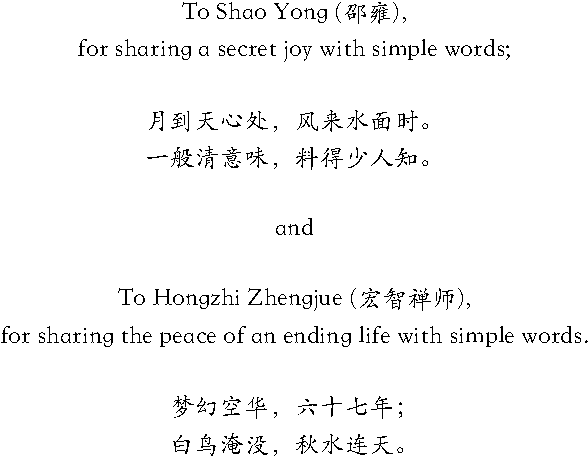
\includegraphics{images/dedication.pdf}
\end{center}

\setlength{\abovedisplayskip}{-5pt}
\setlength{\abovedisplayshortskip}{-5pt}

{
\hypersetup{linkcolor=}
\setcounter{tocdepth}{2}
\tableofcontents
}
\mainmatter

\hypertarget{introduction}{%
\chapter{Introduction}\label{introduction}}

\hypertarget{why-interactive-web-graphics-from-r}{%
\section{\texorpdfstring{Why interactive web graphics \emph{from R}?}{Why interactive web graphics from R?}}\label{why-interactive-web-graphics-from-r}}

As \citet{r4ds} argue, the exploratory phase of a data science workflow (Figure \ref{fig:workflow}) requires lots of iteration between data manipulation, visualization, and modeling. Achieving these tasks through a programming language like \texttt{R} offers the opportunity to scale and automate tasks, document and track them, and reliably reproduce their output. That power, however, typically comes at the cost of increasing the amount of cognitive load involved relative to a GUI-based system.\footnote{For more on the benefits of using code over a GUI to perform data analysis, see \citet{data-science-gui}.} \texttt{R} packages like the \textbf{tidyverse} have been incredibly successful due to their ability to limit cognitive load without removing the benefits of performing analysis via code. Moreover, the \textbf{tidyverse}'s unifying principles of designing for humans, consistency, and composability makes iteration within and between these stages seamless -- an important but often overlooked challenge in exploratory data analysis (EDA) \citep{tidy-principles}.

\begin{figure}

{\centering 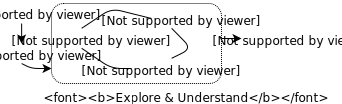
\includegraphics[width=\textwidth]{images/workflow} 

}

\caption{The stages of a data science workflow from \citet{r4ds}.}\label{fig:workflow}
\end{figure}

In fact, packages within the \textbf{tidyverse} such as \textbf{dplyr} (transformation) and \textbf{ggplot2} (visualization) are such productive tools that many analysts use \emph{static} \textbf{ggplot2} graphics for EDA. Then, when it comes to communicating results, some analysts switch to another tool or language altogether (e.g., JavaScript) to generate interactive web graphics presenting their most important findings \citep{flowingdata-r, nyt-r}. Unfortunately, this requires a heavy context switch that requires a totally different skillset and impedes productivity. Moreover, for the average analyst, the opportunity costs involved with becoming competent with the complex world of web technologies is simply not worth the required investment.

Even before the web, interactive graphics were shown to have great promise in aiding the exploration of high-dimensional data \citep{Cook:2007uk}. The ASA maintains an incredible video library, \url{http://stat-graphics.org/movies/}, documenting the use of interactive statistical graphics for tasks that otherwise wouldn't have been easy or possible using numerical summaries and/or static graphics alone. Roughly speaking, these tasks tend to fall under three categories:

\begin{itemize}
\tightlist
\item
  Identifying structure that would otherwise go missing \citep{prim9}.
\item
  Diagnosing models and understanding algorithms \citep{model-vis-paper}.
\item
  Aiding the sense-making process by searching for information quickly without fully specified questions \citep{Unwin:1999vp}.
\end{itemize}

Today, you can find and run some of these and similar Graphical User Interface (GUI) systems for creating interactive graphics: \texttt{DataDesk} \url{https://datadescription.com/}, \texttt{GGobi} \url{http://www.ggobi.org/}, \texttt{Mondrian} \url{http://www.theusrus.de/Mondrian/}, \texttt{JMP} \url{https://www.jmp.com}, \texttt{Tableau} \url{https://www.tableau.com/}. Although these GUI-based systems have nice properties, they don't gel with a code-based workflow: any tasks you complete through a GUI likely can't be replicated without human intervention. That means, if at any point, the data changes, and analysis outputs must be regenerated, you need to remember precisely how to reproduce the outcome, which isn't necessarily easy, trustworthy, or economical. Moreover, GUI-based systems are typically `closed' systems that don't allow themselves to be easily customized, extended, or integrated with another system.

Programming interactive graphics allows you to leverage all the benefits of a code-based workflow while also helping with tasks that are difficult to accomplish with code alone. For an example, if you were to visualize engine displacement (\texttt{displ}) versus miles per gallon (\texttt{hwy}) using the \texttt{mpg} dataset, you might wonder: ``what are these cars with an unusually high value of \texttt{hwy} given their \texttt{displ}?''. Rather than trying to write code to query those observations, it would be more easier and intuitive to draw an outline around the points to query the data behind them.

\begin{Shaded}
\begin{Highlighting}[]
\KeywordTok{library}\NormalTok{(ggplot2)}
\KeywordTok{ggplot}\NormalTok{(mpg, }\KeywordTok{aes}\NormalTok{(displ, hwy)) }\OperatorTok{+}\StringTok{ }\KeywordTok{geom_point}\NormalTok{()}
\end{Highlighting}
\end{Shaded}

\begin{figure}

{\centering 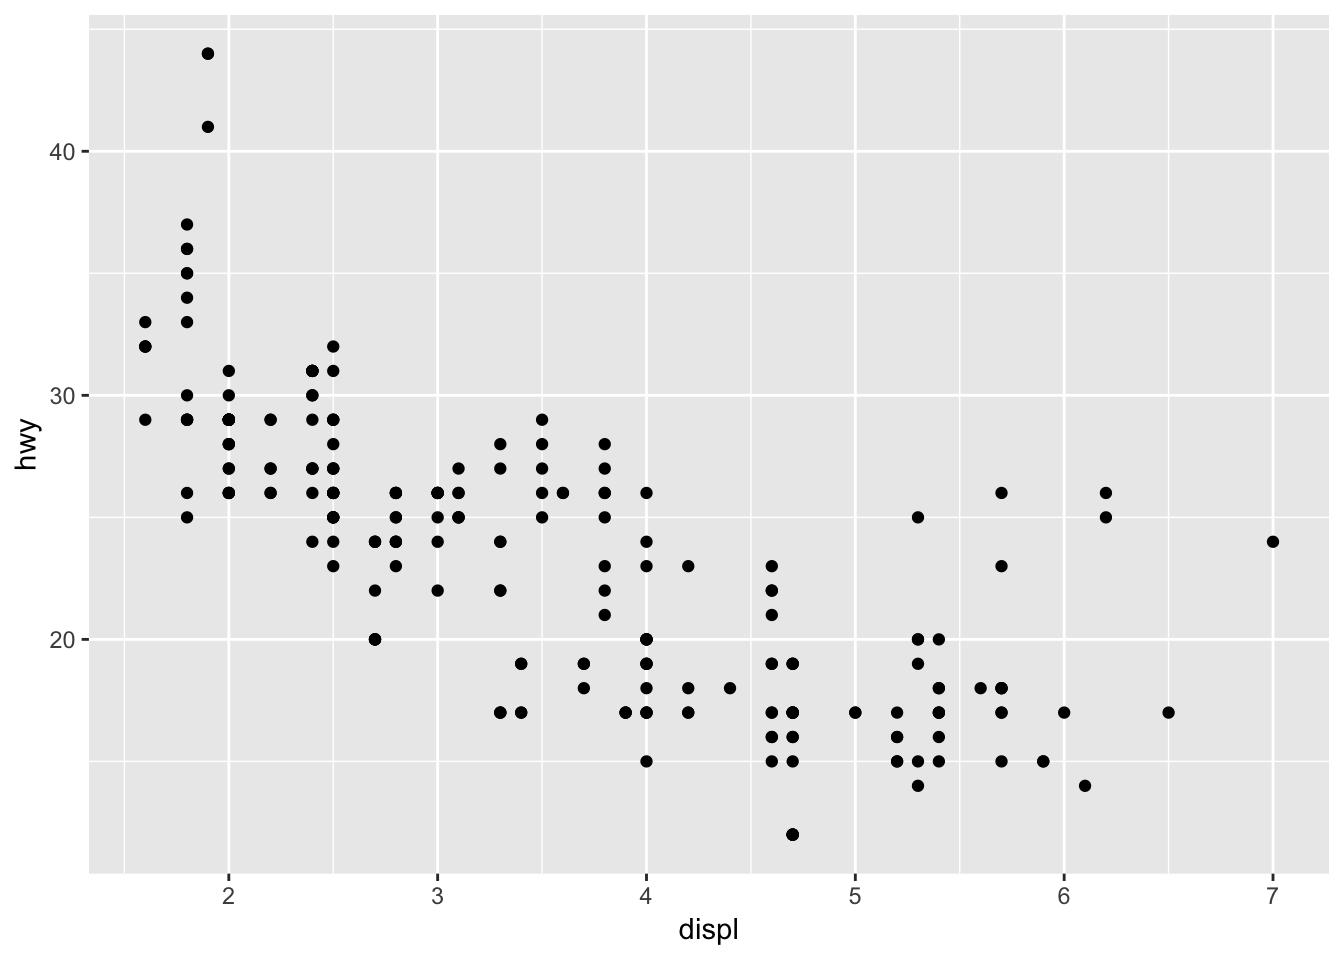
\includegraphics[width=\textwidth]{plotly_book_files/figure-latex/mpg-static-1} 

}

\caption{A scatterplot of engine displacement versus miles per gallon made with the \textbf{ggplot2} package.}\label{fig:mpg-static}
\end{figure}

Figure \ref{fig:mpg-lasso} demonstrates how we can transform Figure \ref{fig:mpg-static} into an interactive version that can be used to query and inspect points of interest. The framework that enables this kind of linked brushing is discussed in depth within Section \ref{graphical-queries}, but the point here is that the added effort required to enable such functionality is relatively small. This is important, because although interactivity \emph{can} augment exploration by allowing us to pursue follow-up questions, it's typically only \emph{practical} when we can create and alter them quickly. That's because, in a true exploratory setting, you have to make lots of visualizations, and investigate lots of follow-up questions, before stumbling across something truly valuable.

\begin{Shaded}
\begin{Highlighting}[]
\KeywordTok{library}\NormalTok{(plotly)}
\NormalTok{m <-}\StringTok{ }\KeywordTok{highlight_key}\NormalTok{(mpg)}
\NormalTok{p <-}\StringTok{ }\KeywordTok{ggplot}\NormalTok{(m, }\KeywordTok{aes}\NormalTok{(displ, hwy)) }\OperatorTok{+}\StringTok{ }\KeywordTok{geom_point}\NormalTok{()}
\NormalTok{gg <-}\StringTok{ }\KeywordTok{highlight}\NormalTok{(}\KeywordTok{ggplotly}\NormalTok{(p), }\StringTok{"plotly_selected"}\NormalTok{)}
\NormalTok{crosstalk}\OperatorTok{::}\KeywordTok{bscols}\NormalTok{(gg, DT}\OperatorTok{::}\KeywordTok{datatable}\NormalTok{(m))}
\end{Highlighting}
\end{Shaded}

\begin{figure}

{\centering 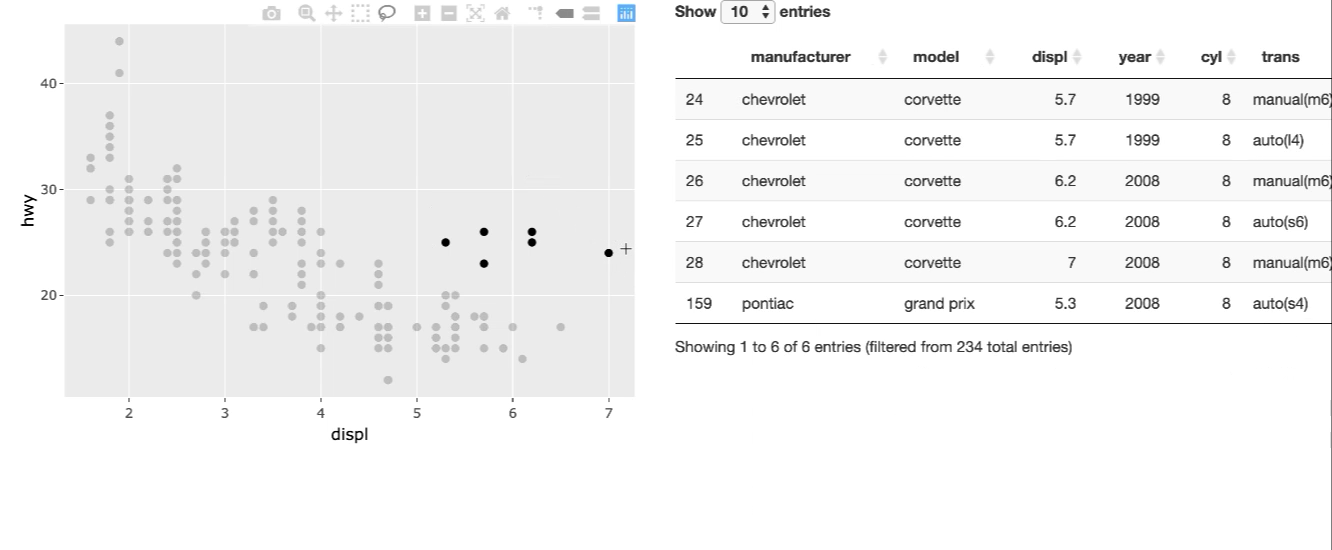
\includegraphics[width=\textwidth]{vimeo-images/324366759/final} 

}

\caption{Linked brushing in a scatterplot to query more information about points of interest. By lasso selecting a region of unusual points, we learn that corvette's have an unusually high miles per gallon considering the engine size. For a video demonstration of the interactive, see \url{https://bit.ly/mpg-lasso}. For the interactive, see \url{https://plotly-r.com/interactives/mpg-lasso.html}}\label{fig:mpg-lasso}
\end{figure}

When a valuable insight surfaces, since the code behind Figure \ref{fig:mpg-lasso} generates HTML, the web-based graphic can be easily shared with collaborators through email and/or incorporated inside a larger automated report or website. Moreover, since these interactive graphics are based on the \textbf{htmlwidgets} framework, they work seamlessly inside of larger \textbf{rmarkdown} documents, inside \textbf{shiny} apps, \texttt{RStudio}, \texttt{Jupyter} notebooks, the \texttt{R} prompt, and more. Being able to share interactive graphics with collaborators through these different mediums enhances the conversation -- your colleagues can point out things you may not yet have considered and, in some cases, they can get immediate responses from the graphics themselves.

In the final stages of an analysis, when it comes time to publish your work to a general audience, rather than relying on the audience to interact with the graphics and discover insight for themselves, it's always a good idea to clearly highlight your findings. For example, from Figure \ref{fig:mpg-lasso}, we've learned that most of these unusual points can be explained by a single feature of the data (\texttt{model\ ==\ \textquotesingle{}corvette\textquotesingle{}}). As shown in Figure \ref{fig:mpg-mark-hull}, the \texttt{geom\_mark\_hull()} function from the \textbf{ggforce} package provides a helpful way to annotate those points with a hull. Moreover, as Chapter \ref{editing-views} demonstrates, it can also be helpful to add and/or edit annotations interactively when preparing a graphic for publication.

\begin{Shaded}
\begin{Highlighting}[]
\KeywordTok{library}\NormalTok{(ggforce)}
\KeywordTok{ggplot}\NormalTok{(mpg, }\KeywordTok{aes}\NormalTok{(displ, hwy)) }\OperatorTok{+}\StringTok{ }
\StringTok{  }\KeywordTok{geom_point}\NormalTok{() }\OperatorTok{+}
\StringTok{  }\KeywordTok{geom_mark_hull}\NormalTok{(}\KeywordTok{aes}\NormalTok{(}\DataTypeTok{filter =}\NormalTok{ model }\OperatorTok{==}\StringTok{ "corvette"}\NormalTok{, }\DataTypeTok{label =}\NormalTok{ model)) }\OperatorTok{+}
\StringTok{  }\KeywordTok{labs}\NormalTok{(}
    \DataTypeTok{title =} \StringTok{"Fuel economy from 1999 to 2008 for 38 car models"}\NormalTok{,}
    \DataTypeTok{caption =} \StringTok{"Source: https://fueleconomy.gov/"}\NormalTok{,}
    \DataTypeTok{x =} \StringTok{"Engine Displacement"}\NormalTok{, }
    \DataTypeTok{y =} \StringTok{"Miles Per Gallon"}
\NormalTok{  )}
\end{Highlighting}
\end{Shaded}

\begin{figure}

{\centering 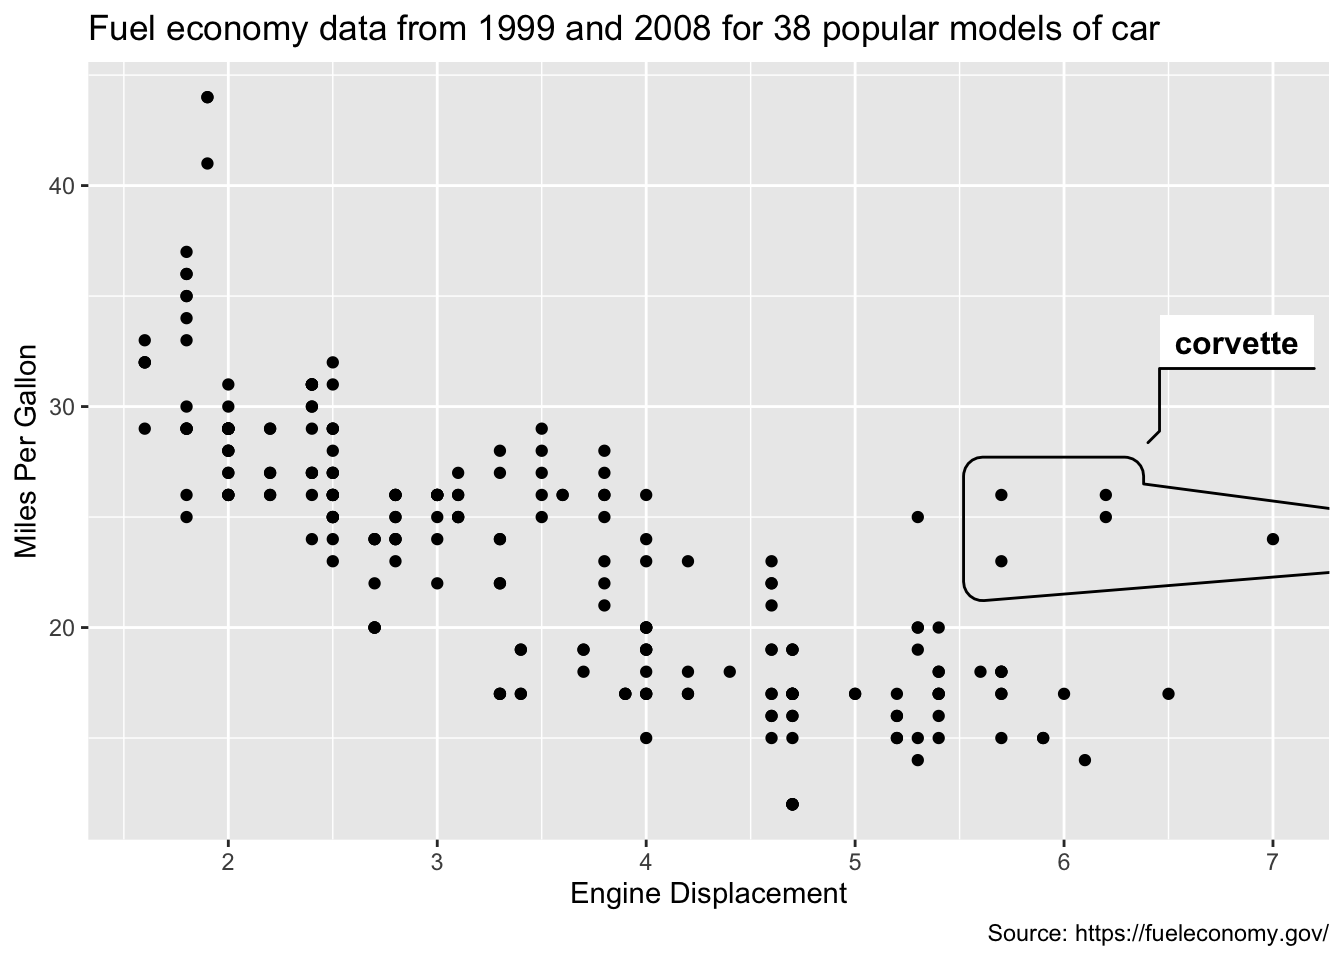
\includegraphics[width=\textwidth]{plotly_book_files/figure-latex/mpg-mark-hull-1} 

}

\caption{Using the \textbf{ggforce} package to annotate the corvette's in this dataset.}\label{fig:mpg-mark-hull}
\end{figure}

This simple example quickly shows how interactive web graphics can assist EDA (for another, slightly more in-depth example, see Section \ref{intro-ggplotly}). Being able to program these graphics from \texttt{R} allows one to combine their functionality within a world-class computing environment for data analysis and statistics. Programming interactive graphics may not be as intuitive as using a GUI-based system, but making the investment pays dividends in terms of workflow improvements: automation, scaling, provenance, and flexibility.

\hypertarget{what-you-will-learn}{%
\section{What you will learn}\label{what-you-will-learn}}

This book provides a foundation for learning how to make interactive web-based graphics for data analysis from \texttt{R} via \textbf{plotly}, without assuming any prior experience with web technologies. The goal is to provide the context you need to go beyond copying existing \textbf{plotly} examples to having a useful mental model of the underlying framework, its capabilities, and how it fits into the larger R ecosystem. By learning this mental model, you'll have a better understanding of how to create more sophisticated visualizations, fix common issues, improve performance, understand the limitations, and even contribute back to the project itself. You may already be familiar with existing \textbf{plotly} documentation (e.g., \url{https://plot.ly/r/}), which is essentially a language-agnostic how-to guide, but this book is meant to be more holistic tutorial written by and for the R user.

This book also focuses primarily on features that are unique to the \textbf{plotly} R package (i.e., things that don't work the same for Python or JavaScript). This ranges from creation of a single graph using the \texttt{plot\_ly()} special named arguments that make it easier to map data to visuals:

\begin{Shaded}
\begin{Highlighting}[]
\KeywordTok{plot_ly}\NormalTok{(diamonds, }\DataTypeTok{x =} \OperatorTok{~}\NormalTok{cut, }\DataTypeTok{color =} \OperatorTok{~}\NormalTok{clarity, }\DataTypeTok{colors =} \StringTok{"Accent"}\NormalTok{)}
\end{Highlighting}
\end{Shaded}

\begin{figure}

{\centering 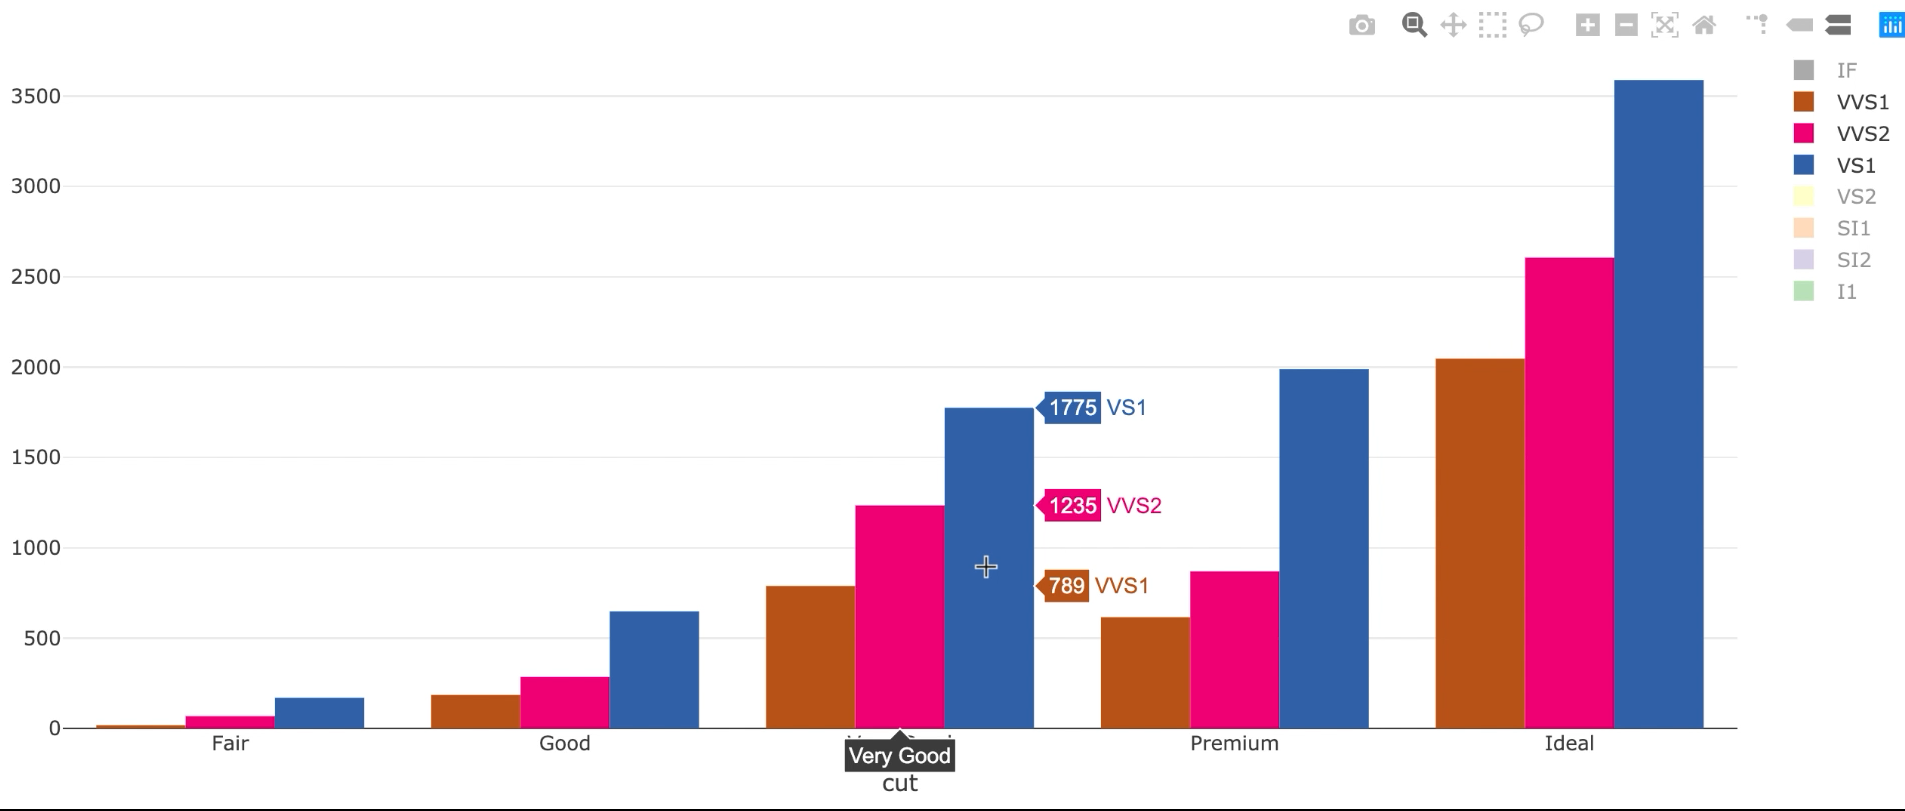
\includegraphics[width=\textwidth]{vimeo-images/315707813/final} 

}

\caption{An example of what you'll learn: Figure \ref{fig:intro-show-hide}. For a video demonstration of the interactive, see \url{https://bit.ly/intro-show-hide-preview}. For the interactive, see \url{https://plotly-r.com/interactives/intro-show-hide-preview.html}}\label{fig:intro-show-hide-preview}
\end{figure}

To its ability to link multiple data views purely client-side (see Section \ref{graphical-queries}):

\begin{figure}

{\centering 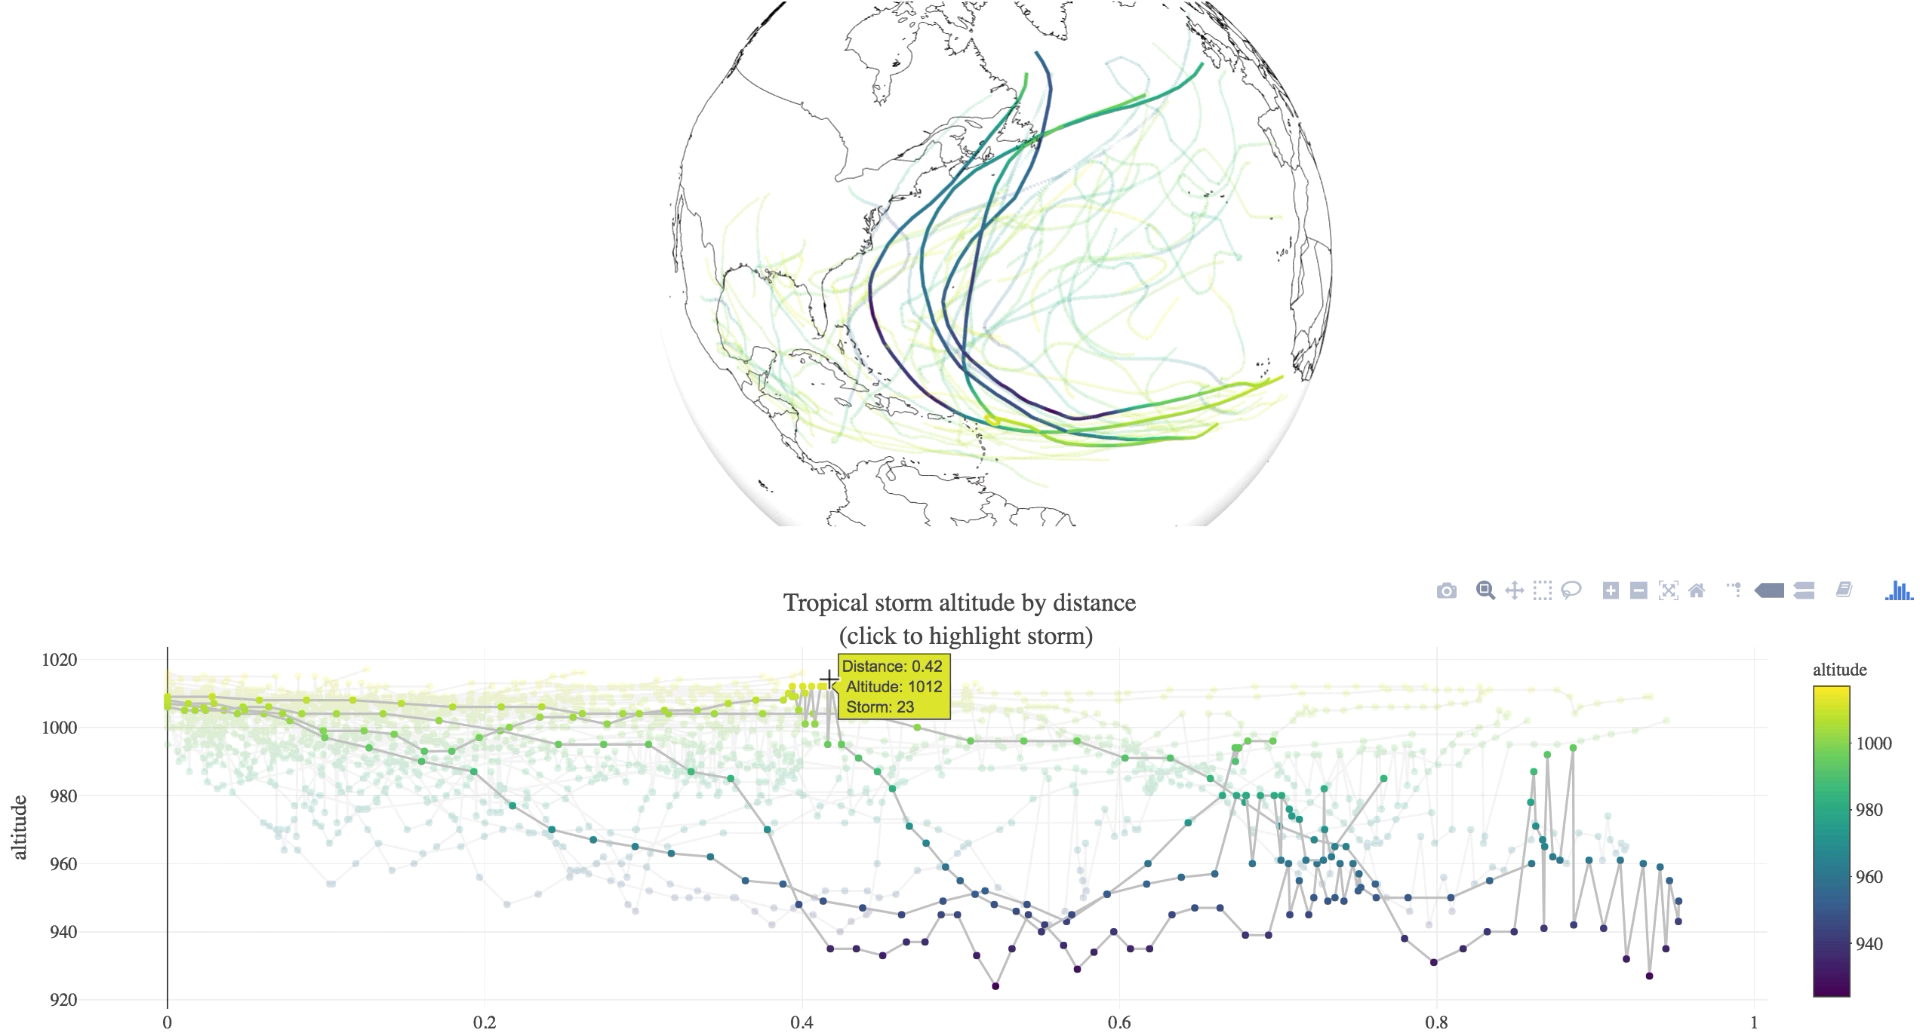
\includegraphics[width=\textwidth]{vimeo-images/257149623/final} 

}

\caption{An example of what you'll learn: Figure \ref{fig:storms}. For a video demonstration of the interactive, see \url{https://bit.ly/storms-preview}. For the interactive, see \url{https://plotly-r.com/interactives/storms-preview.html}}\label{fig:storms-preview}
\end{figure}

To advanced server-side linking with \textbf{shiny} to implement responsive and scalable crossfilters (see Section \ref{crossfilter}):

\begin{figure}

{\centering 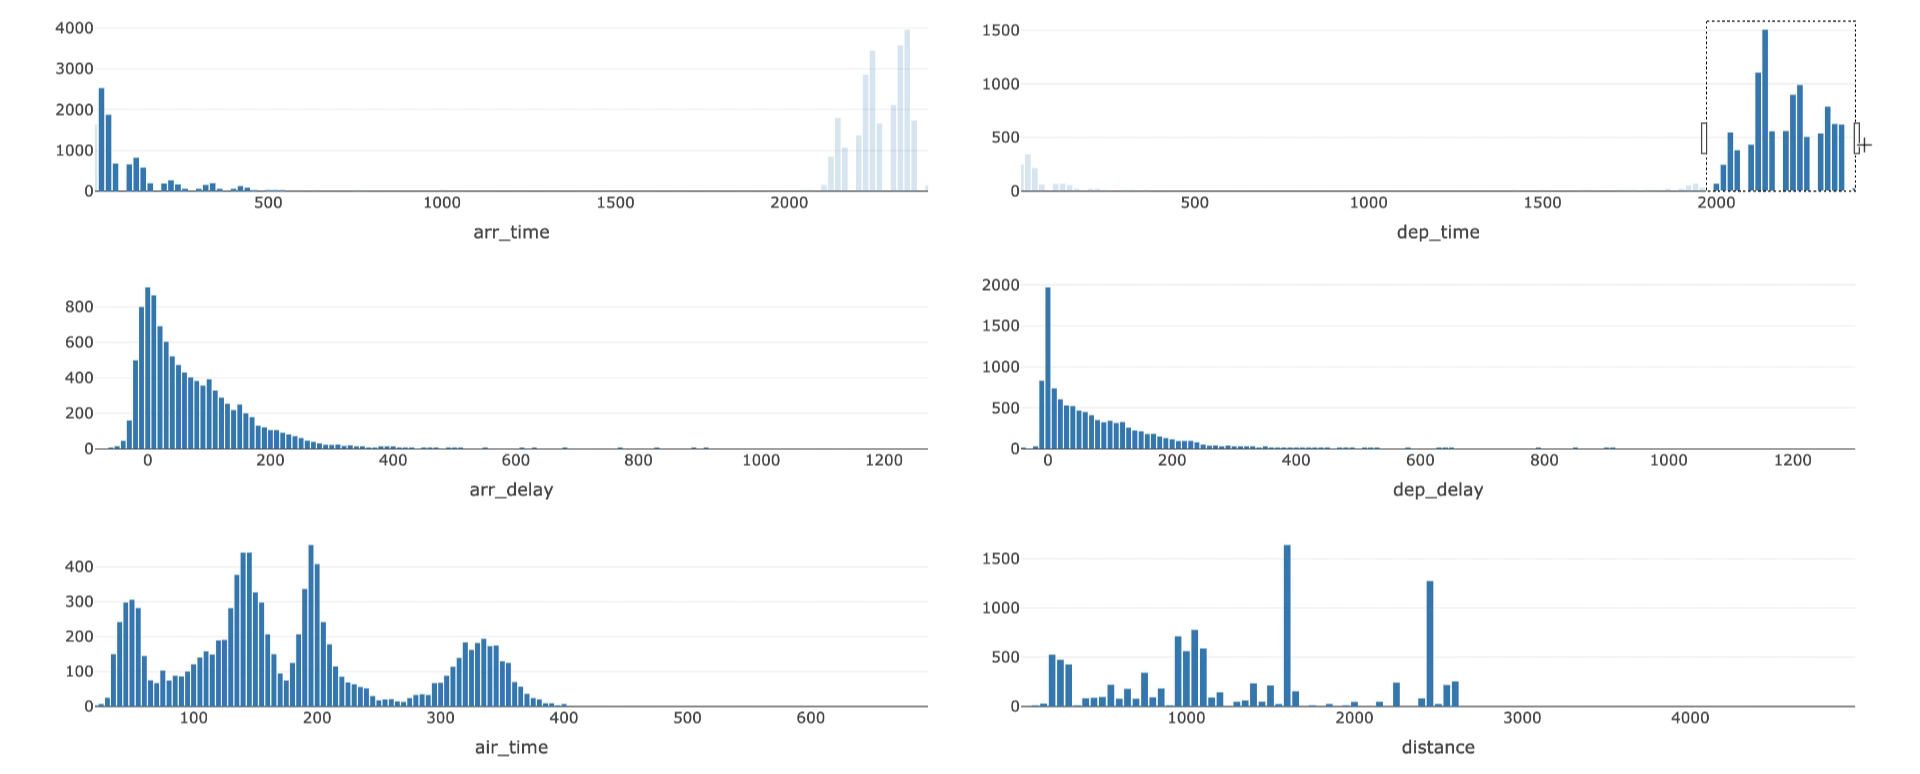
\includegraphics[width=\textwidth]{vimeo-images/318129502/final} 

}

\caption{An example of what you'll learn: Figure \ref{fig:shiny-crossfilter}. For a video demonstration of the interactive, see \url{https://bit.ly/shiny-crossfilter-preview}. For the interactive, see \url{https://plotly-r.com/interactives/shiny-crossfilter-preview.html}}\label{fig:shiny-crossfilter-preview}
\end{figure}

By going through the code behind these examples, you'll see that many of them leverage other \texttt{R} packages in their implementation. To highlight a few of the R packages that you'll see:

\begin{itemize}
\tightlist
\item
  \textbf{dplyr} and \textbf{tidyr}

  \begin{itemize}
  \tightlist
  \item
    For transforming data into a form suitable for the visualization method.
  \end{itemize}
\item
  \textbf{ggplot2} and friends (e.g., \textbf{GGally}, \textbf{ggmosaic}, etc)

  \begin{itemize}
  \tightlist
  \item
    For creating \textbf{plotly} visualizations that would be tedious to implement without \texttt{ggplotly()}.
  \end{itemize}
\item
  \textbf{sf}, \textbf{rnaturalearth}, \textbf{cartogram}

  \begin{itemize}
  \tightlist
  \item
    For obtaining and working with geo-spatial data structures in R.
  \end{itemize}
\item
  \textbf{stats}, \textbf{MASS}, \textbf{broom}, and \textbf{forecast}

  \begin{itemize}
  \tightlist
  \item
    For working with statistical models and summaries.
  \end{itemize}
\item
  \textbf{shiny}

  \begin{itemize}
  \tightlist
  \item
    For running R code in response to user input.
  \end{itemize}
\item
  \textbf{htmltools}, \textbf{htmlwidgets}

  \begin{itemize}
  \tightlist
  \item
    For combining multiple views and saving the result.
  \end{itemize}
\end{itemize}

This book contains six parts and each part contains numerous chapters. A summary of each part is provided below.

\begin{enumerate}
\def\labelenumi{\arabic{enumi}.}
\item
  \emph{Creating views:} introduces the process of transforming data into graphics via \textbf{plotly}'s programmatic interface. It focuses mostly on \texttt{plot\_ly()}, which can interface directly with the underlying plotly.js graphing library, but emphasis is put on features unique to the \texttt{R} package that make it easier to transform data into graphics. Another way to create graphs with \textbf{plotly} is to use the \texttt{ggplotly()} function to transform \textbf{ggplot2} graphs into \textbf{plotly} graphs. Section \ref{intro-ggplotly} discusses when and why \texttt{ggplotly()} might be desirable to \texttt{plot\_ly()}. It's also worth mentioning that this part (nor the book as a whole) does not intend to cover every possible chart type and option available in \textbf{plotly} -- it's more of a presentation of the most generally useful techniques with the greater \texttt{R} ecosystem in mind. For a more exhaustive gallery of examples of what \textbf{plotly} itself is capable of, see \url{https://plot.ly/r/}.
\item
  \emph{Publishing views:} discusses various techniques for exporting (as well as embedding) \textbf{plotly} graphs to various file formats (e.g., HTML, svg, pdf, png, etc). Also, Chapter \ref{editing-views} demonstrates how one could leverage editable layout components HTML to touch-up a graph, then export to a static file format of interest before publication. Indeed, this book was created using the techniques from this section.
\item
  \emph{Combining multiple views:} demonstrates how to combine multiple data views into a single web page (arranging) or graphic (animation). Most of these techniques are shown using \textbf{plotly} graphs, but techniques from Section \ref{arranging-htmlwidgets} extend to any HTML content generated via \textbf{htmltools} (which includes \textbf{htmlwidgets}).
\item
  \emph{Linking multiple views:} provides an overview of the two models for linking \textbf{plotly} graph(s) to other data views. The first model, covered in Section \ref{graphical-queries}, outlines \textbf{plotly}'s support for linking views purely client-side, meaning the resulting graphs render in any web browser on any machine without requiring external software. The second model, covered in Chapter \ref{linking-views-with-shiny}, demonstrates how to link \textbf{plotly} with other views via \textbf{shiny}, a reactive web application framework for \texttt{R}. Relatively speaking, the second model grants the \texttt{R} user way more power and flexibility, but comes at the cost of requiring more computational infrastructure. That being said, RStudio provides accessible resources for deploying \textbf{shiny} apps \url{https://shiny.rstudio.com/articles/\#deployment}.
\item
  \emph{Custom behavior with JavaScript:} demonstrates various ways to customize \textbf{plotly} graphs by writing custom JavaScript to handle certain user events. This part of the book is designed to be approachable for \texttt{R} users that want to learn just enough JavaScript to \textbf{plotly} to do something it doesn't ``natively'' support.
\item
  \emph{Various special topics}: offers a grab-bag of topics that address common questions, mostly related to the customization of \textbf{plotly} graphs in \texttt{R}.
\end{enumerate}

You might already notice that this book often uses the term `view' or `data view', so here we take a moment to frame its use in a wider context. As \citet{Wills2008} puts it: ``a `data view' is anything that gives the user a way of examining data so as to gain insight and understanding. A data view is usually thought of as a barchart, scatterplot, or other traditional statistical graphic, but we use the term more generally, including `views' such as the results of a regression analysis, a neural net prediction, or a set of descriptive statistics''. In this book, more often than not, the term `view' typically refers to a \textbf{plotly} graph or other \textbf{htmlwidgets} (e.g., \textbf{DT}, \textbf{leaflet}, etc). In particular, Section \ref{graphical-queries} is all about linking multiple \textbf{htmlwidgets} together through a graphical database querying framework. However, the term `view' takes on a more general interpretation in Chapter \ref{linking-views-with-shiny} since the reactive programming framework that \textbf{shiny} provides allows us to have a more general conversation surrounding linked data views.

\hypertarget{what-you-wont-learn-much-of}{%
\section{What you won't learn (much of)}\label{what-you-wont-learn-much-of}}

\hypertarget{web-technologies}{%
\subsection{Web technologies}\label{web-technologies}}

Although this book is fundamentally about creating web graphics, it does not aim to teach you web technologies (e.g., HTML, SVG, CSS, JavaScript, etc). It's true that mastering these technologies grants you the ability to build really impressive websites, but even expert web developers would say their skillset is much better suited for expository rather than exploratory visualization. That's because, most web programming tools are not well-suited for the exploratory phase of a data science workflow where iteration between data visualization, transformation, and modeling is a necessary task that often impedes hypothesis generation and sense-making. As a result, for most data analysts whose primary function is to derive insight from data, the opportunity costs involved with mastering web technologies is usually not worth the investment.

That being said, learning a little about web technologies can have a relatively large payoff with directed learning and instruction. In Chapter \ref{javascript}, you'll learn how to customize \textbf{plotly} graphs with JavaScript -- even if you haven't seen JavaScript before, this chapter should be approachable, insightful, and provide you with some useful examples.

\hypertarget{d3js}{%
\subsection{d3js}\label{d3js}}

The JavaScript library D3 is a great tool for data visualization assuming you're familiar with web technologies and are primarily interested in expository (not exploratory) visualization. There are already lots of great resources for learning D3, including the numerous books by \citet{murray-d3} and \citet{meeks-d3}. It's worth noting, however, if you do know D3, you can easily leverage it from a web page that are already a \textbf{plotly} graph, as demonstrated in Figure \ref{fig:correlation-client-side}.

\hypertarget{ggplot2}{%
\subsection{ggplot2}\label{ggplot2}}

The book does contain some \textbf{ggplot2} code examples (which are then converted to \textbf{plotly} via \texttt{ggplotly()}), but it's not designed to teach you \textbf{ggplot2}. For those looking to learn \textbf{ggplot2}, I recommend using the learning materials listed at \url{https://ggplot2.tidyverse.org}.

\hypertarget{graphical-data-analysis}{%
\subsection{Graphical data analysis}\label{graphical-data-analysis}}

How to perform data analysis via graphics (carefully, correctly, and creatively) is a large topic unto itself. Although this book does have examples of graphical data analysis, it does not aim to provide a comprehensive foundation. For nice comprehensive resources on the topic, see \citet{unwin-graphical-analysis} and \citet{ggobi:2007}.

\hypertarget{data-visualization-best-practices}{%
\subsection{Data visualization best practices}\label{data-visualization-best-practices}}

Encoding information in a graphic (concisely and effectively) is a large topic unto itself. Although this book does have some ramblings related to best practices in data visualization, it does not aim to provide a comprehensive foundation. For some approachable and fun resources on the topic, see \citet{tufte-dataviz}, \citet{yau-dataviz}, \citet{healey-dataviz}, and \citet{claus-dataviz}.

\hypertarget{prerequisites}{%
\section{Prerequisites}\label{prerequisites}}

For those new to \texttt{R} and/or data visualization, \href{https://r4ds.had.co.nz/}{R for Data Science} provides an excellent foundation for understanding the vast majority of concepts covered in this book \citep{r4ds}. In particular, if you have a solid grasp on \href{https://r4ds.had.co.nz/explore-intro.html}{Part I: Explore}, \href{https://r4ds.had.co.nz/wrangle-intro.html}{Part II: Wrangle}, and \href{https://r4ds.had.co.nz/program-intro.html}{Part III: Program}, you should be able to understand almost everything here. Although not explicitly covered, the book does make references to (and was creating using) \textbf{rmarkdown}, so if you're new to \textbf{rmarkdown}, I also recommend reading the \href{https://r4ds.had.co.nz/r-markdown.html}{R Markdown chapter}.

\hypertarget{run-code-examples}{%
\section{Run code examples}\label{run-code-examples}}

This book contains many code examples in an effort to teach the art and science behind creating interactive web-based graphics using \textbf{plotly}. To see the actual interactive result of the code (rather than a video or static version), you may want to run the code examples in a suitable computational environment. Visit \url{http://bit.ly/plotly-book-cloud} for a cloud-based instance of RStudio with all the required software to run the code examples in this book. Most, if not all of these code examples assume you have the \textbf{plotly} package loaded:

\begin{Shaded}
\begin{Highlighting}[]
\KeywordTok{library}\NormalTok{(plotly)}
\end{Highlighting}
\end{Shaded}

Within some chapters, there may be examples that assume packages we loaded during a previous example. If you'd like to avoid this situation, please load the

\begin{Shaded}
\begin{Highlighting}[]
\KeywordTok{library}\NormalTok{(plotlyBook)}
\end{Highlighting}
\end{Shaded}

If you'd like to run examples on your local machine (instead of RStudio Cloud), you can install all the necessary R packages with:

\begin{Shaded}
\begin{Highlighting}[]
\ControlFlowTok{if}\NormalTok{ (}\OperatorTok{!}\KeywordTok{require}\NormalTok{(remotes)) }\KeywordTok{install.packages}\NormalTok{(}\StringTok{"remotes"}\NormalTok{)}
\NormalTok{remotes}\OperatorTok{::}\KeywordTok{install_github}\NormalTok{(}\StringTok{"cpsievert/plotly_book"}\NormalTok{)}
\end{Highlighting}
\end{Shaded}

\hypertarget{getting-help-and-learning-more}{%
\section{Getting help and learning more}\label{getting-help-and-learning-more}}

As \citet{r4ds} states, ``This book is not an island; there is no single resource that will allow you to master \texttt{R} {[}or \textbf{plotly}{]}. As you start to apply the techniques described in this book to your own data you will soon find questions that I do not answer. This section describes a few tips on how to get help, and to help you keep learning.'' \href{https://r4ds.had.co.nz/introduction.html\#getting-help-and-learning-more}{These tips} on how to get help (e.g., Google, StackOverflow, Twitter, etc) also apply to getting help with \textbf{plotly}. \href{https://community.rstudio.com/tags/plotly}{RStudio's community} is another great place to ask broader questions about all things \texttt{R} and \textbf{plotly}. It's worth mentioning that the \texttt{R} community is incredibly welcoming, compassionate, and generous; especially if you can demonstrate that you've done your research and/or \href{https://www.tidyverse.org/help/}{provide minimally reproducible example of your problem}.

\hypertarget{acknowledgements}{%
\section{Acknowledgements}\label{acknowledgements}}

This book wouldn't be possible without the generous assistance and mentorship of many people:

\begin{itemize}
\tightlist
\item
  Heike Hofmann and Di Cook for their mentorship and many helpful conversations about interactive graphics.
\item
  Toby Dylan Hocking for many helpful conversations, his mentorship in the \texttt{R} packages \textbf{animint} and \textbf{plotly}, and laying the original foundation behind \texttt{ggplotly()}.
\item
  Joe Cheng for many helpful conversations and inspiring Section \ref{graphical-queries}.
\item
  Étienne Tétreault-Pinard, Alex Johnson, and the other plotly.js core developers for responding to my feature requests and bug reports.
\item
  Yihui Xie for his work on \textbf{knitr}, \textbf{rmarkdown}, \textbf{bookdown}, \href{https://github.com/yihui/bookdown-crc}{bookdown-crc}, and responding to my feature requests.
\item
  Anthony Unwin for helpful feedback, suggestions, and for inspiring Figure \ref{fig:epl}.
\item
  Hadley Wickham and the \textbf{ggplot2} team for maintaining \textbf{ggplot2}.
\item
  Hadley Wickham and Garret Grolemund for writing \emph{R for Data Science} and allowing me to model this introduction after their introduction.
\item
  Kent Russell for contributions to \textbf{plotly} and writing \textbf{reactR}.
\item
  Adam Loy for inspiring Figure \ref{fig:profile-pyramid}.
\item
  Many other R community members who contributed to the \textbf{plotly} package and provided feedback and corrections for this book.
\end{itemize}

\hypertarget{colophon}{%
\section{Colophon}\label{colophon}}

An online version of this book is available at \url{https://plotly-r.com}. It will continue to evolve in between reprints of the physical book. The source of the book is available at \url{https://github.com/cpsievert/plotly_book}. The book is powered by \url{https://bookdown.org} which makes it easy to turn \texttt{R} markdown files into HTML, PDF, and EPUB.

This book was built with the following computing environment:

\begin{Shaded}
\begin{Highlighting}[]
\NormalTok{devtools}\OperatorTok{::}\KeywordTok{session_info}\NormalTok{(}\StringTok{"plotly"}\NormalTok{)}
\CommentTok{#> - Session info --------------------------------------}
\CommentTok{#>  setting  value                       }
\CommentTok{#>  version  R version 3.6.1 (2019-07-05)}
\CommentTok{#>  os       macOS Mojave 10.14.5        }
\CommentTok{#>  system   x86_64, darwin15.6.0        }
\CommentTok{#>  ui       X11                         }
\CommentTok{#>  language (EN)                        }
\CommentTok{#>  collate  en_US.UTF-8                 }
\CommentTok{#>  ctype    en_US.UTF-8                 }
\CommentTok{#>  tz       America/Chicago             }
\CommentTok{#>  date     2019-10-02                  }
\CommentTok{#> }
\CommentTok{#> - Packages ------------------------------------------}
\CommentTok{#>  package      * version    date       lib}
\CommentTok{#>  askpass        1.1        2019-01-13 [1]}
\CommentTok{#>  assertthat     0.2.1      2019-03-21 [1]}
\CommentTok{#>  backports      1.1.4      2019-04-10 [1]}
\CommentTok{#>  base64enc      0.1-3      2015-07-28 [1]}
\CommentTok{#>  BH             1.69.0-1   2019-01-07 [1]}
\CommentTok{#>  cli            1.1.0      2019-03-19 [1]}
\CommentTok{#>  colorspace     1.4-1      2019-03-18 [1]}
\CommentTok{#>  crayon         1.3.4      2017-09-16 [1]}
\CommentTok{#>  crosstalk      1.0.0      2016-12-21 [1]}
\CommentTok{#>  curl           4.2        2019-09-24 [1]}
\CommentTok{#>  data.table     1.12.2     2019-04-07 [1]}
\CommentTok{#>  digest         0.6.21     2019-09-20 [1]}
\CommentTok{#>  dplyr          0.8.3      2019-07-04 [1]}
\CommentTok{#>  ellipsis       0.3.0      2019-09-20 [1]}
\CommentTok{#>  fansi          0.4.0      2018-10-05 [1]}
\CommentTok{#>  fastmap        1.0.0      2019-08-02 [1]}
\CommentTok{#>  ggplot2      * 3.2.1.9000 2019-10-01 [1]}
\CommentTok{#>  glue           1.3.1      2019-03-12 [1]}
\CommentTok{#>  gtable         0.3.0      2019-03-25 [1]}
\CommentTok{#>  hexbin         1.27.3     2019-05-14 [1]}
\CommentTok{#>  htmltools      0.4.0      2019-09-17 [1]}
\CommentTok{#>  htmlwidgets    1.4.0.9000 2019-10-01 [1]}
\CommentTok{#>  httpuv         1.5.2      2019-09-11 [1]}
\CommentTok{#>  httr           1.4.1      2019-08-05 [1]}
\CommentTok{#>  jsonlite       1.6        2018-12-07 [1]}
\CommentTok{#>  labeling       0.3        2014-08-23 [1]}
\CommentTok{#>  later          1.0.0      2019-09-17 [1]}
\CommentTok{#>  lattice        0.20-38    2018-11-04 [1]}
\CommentTok{#>  lazyeval       0.2.2      2019-03-15 [1]}
\CommentTok{#>  lifecycle      0.1.0      2019-08-01 [1]}
\CommentTok{#>  magrittr       1.5        2014-11-22 [1]}
\CommentTok{#>  MASS           7.3-51.4   2019-03-31 [1]}
\CommentTok{#>  Matrix         1.2-17     2019-03-22 [1]}
\CommentTok{#>  mgcv           1.8-29     2019-09-20 [1]}
\CommentTok{#>  mime           0.7        2019-06-11 [1]}
\CommentTok{#>  munsell        0.5.0      2018-06-12 [1]}
\CommentTok{#>  nlme           3.1-141    2019-08-01 [1]}
\CommentTok{#>  openssl        1.4.1      2019-07-18 [1]}
\CommentTok{#>  pillar         1.4.2      2019-06-29 [1]}
\CommentTok{#>  pkgconfig      2.0.3      2019-09-22 [1]}
\CommentTok{#>  plogr          0.2.0      2018-03-25 [1]}
\CommentTok{#>  plotly         4.9.0      2019-04-10 [1]}
\CommentTok{#>  plyr           1.8.4      2016-06-08 [1]}
\CommentTok{#>  promises       1.1.0      2019-09-25 [1]}
\CommentTok{#>  purrr          0.3.2.9000 2019-09-30 [1]}
\CommentTok{#>  R6             2.4.0      2019-02-14 [1]}
\CommentTok{#>  RColorBrewer   1.1-2      2014-12-07 [1]}
\CommentTok{#>  Rcpp           1.0.2      2019-07-25 [1]}
\CommentTok{#>  reshape2       1.4.3      2017-12-11 [1]}
\CommentTok{#>  rlang          0.4.0.9002 2019-09-25 [1]}
\CommentTok{#>  scales         1.0.0.9000 2019-07-19 [1]}
\CommentTok{#>  shiny          1.4.0      2019-10-01 [1]}
\CommentTok{#>  sourcetools    0.1.7      2018-04-25 [1]}
\CommentTok{#>  stringi        1.4.3      2019-03-12 [1]}
\CommentTok{#>  stringr        1.4.0      2019-02-10 [1]}
\CommentTok{#>  sys            3.3        2019-08-21 [1]}
\CommentTok{#>  tibble         2.1.3      2019-06-06 [1]}
\CommentTok{#>  tidyr          1.0.0      2019-09-11 [1]}
\CommentTok{#>  tidyselect     0.2.5      2018-10-11 [1]}
\CommentTok{#>  utf8           1.1.4      2018-05-24 [1]}
\CommentTok{#>  vctrs          0.2.0.9003 2019-10-01 [1]}
\CommentTok{#>  viridisLite    0.3.0      2018-02-01 [1]}
\CommentTok{#>  withr          2.1.2      2018-03-15 [1]}
\CommentTok{#>  xtable         1.8-4      2019-04-21 [1]}
\CommentTok{#>  yaml           2.2.0      2018-07-25 [1]}
\CommentTok{#>  zeallot        0.1.0      2018-01-28 [1]}
\CommentTok{#>  source                               }
\CommentTok{#>  CRAN (R 3.6.0)                       }
\CommentTok{#>  CRAN (R 3.6.0)                       }
\CommentTok{#>  CRAN (R 3.6.0)                       }
\CommentTok{#>  CRAN (R 3.6.0)                       }
\CommentTok{#>  CRAN (R 3.6.0)                       }
\CommentTok{#>  CRAN (R 3.6.0)                       }
\CommentTok{#>  CRAN (R 3.6.0)                       }
\CommentTok{#>  CRAN (R 3.6.0)                       }
\CommentTok{#>  CRAN (R 3.6.0)                       }
\CommentTok{#>  CRAN (R 3.6.1)                       }
\CommentTok{#>  CRAN (R 3.6.0)                       }
\CommentTok{#>  CRAN (R 3.6.1)                       }
\CommentTok{#>  CRAN (R 3.6.0)                       }
\CommentTok{#>  CRAN (R 3.6.1)                       }
\CommentTok{#>  CRAN (R 3.6.0)                       }
\CommentTok{#>  Github (r-lib/fastmap@b104c2c)       }
\CommentTok{#>  local                                }
\CommentTok{#>  CRAN (R 3.6.0)                       }
\CommentTok{#>  CRAN (R 3.6.0)                       }
\CommentTok{#>  CRAN (R 3.6.0)                       }
\CommentTok{#>  Github (rstudio/htmltools@0366ff7)   }
\CommentTok{#>  Github (ramnathv/htmlwidgets@0ef5dd5)}
\CommentTok{#>  CRAN (R 3.6.1)                       }
\CommentTok{#>  CRAN (R 3.6.1)                       }
\CommentTok{#>  CRAN (R 3.6.0)                       }
\CommentTok{#>  CRAN (R 3.6.0)                       }
\CommentTok{#>  Github (r-lib/later@0364de9)         }
\CommentTok{#>  CRAN (R 3.6.1)                       }
\CommentTok{#>  CRAN (R 3.6.0)                       }
\CommentTok{#>  CRAN (R 3.6.0)                       }
\CommentTok{#>  CRAN (R 3.6.0)                       }
\CommentTok{#>  CRAN (R 3.6.1)                       }
\CommentTok{#>  CRAN (R 3.6.1)                       }
\CommentTok{#>  CRAN (R 3.6.0)                       }
\CommentTok{#>  CRAN (R 3.6.0)                       }
\CommentTok{#>  CRAN (R 3.6.0)                       }
\CommentTok{#>  CRAN (R 3.6.0)                       }
\CommentTok{#>  CRAN (R 3.6.1)                       }
\CommentTok{#>  CRAN (R 3.6.0)                       }
\CommentTok{#>  CRAN (R 3.6.1)                       }
\CommentTok{#>  CRAN (R 3.6.0)                       }
\CommentTok{#>  CRAN (R 3.6.0)                       }
\CommentTok{#>  CRAN (R 3.6.0)                       }
\CommentTok{#>  Github (rstudio/promises@39faf86)    }
\CommentTok{#>  Github (tidyverse/purrr@9edf0ca)     }
\CommentTok{#>  CRAN (R 3.6.0)                       }
\CommentTok{#>  CRAN (R 3.6.0)                       }
\CommentTok{#>  CRAN (R 3.6.1)                       }
\CommentTok{#>  CRAN (R 3.6.0)                       }
\CommentTok{#>  Github (r-lib/rlang@03bc5ed)         }
\CommentTok{#>  Github (r-lib/scales@7f6f4a5)        }
\CommentTok{#>  Github (rstudio/shiny@c8daa17)       }
\CommentTok{#>  CRAN (R 3.6.0)                       }
\CommentTok{#>  CRAN (R 3.6.0)                       }
\CommentTok{#>  CRAN (R 3.6.0)                       }
\CommentTok{#>  CRAN (R 3.6.0)                       }
\CommentTok{#>  CRAN (R 3.6.0)                       }
\CommentTok{#>  CRAN (R 3.6.0)                       }
\CommentTok{#>  CRAN (R 3.6.0)                       }
\CommentTok{#>  CRAN (R 3.6.0)                       }
\CommentTok{#>  Github (r-lib/vctrs@bc20422)         }
\CommentTok{#>  CRAN (R 3.6.0)                       }
\CommentTok{#>  CRAN (R 3.6.0)                       }
\CommentTok{#>  CRAN (R 3.6.0)                       }
\CommentTok{#>  CRAN (R 3.6.0)                       }
\CommentTok{#>  CRAN (R 3.6.0)                       }
\CommentTok{#> }
\CommentTok{#> [1] /Library/Frameworks/R.framework/Versions/3.6/Resources/library}
\end{Highlighting}
\end{Shaded}

\hypertarget{part-creating-views}{%
\part{Creating views}\label{part-creating-views}}

\hypertarget{overview}{%
\chapter{Overview}\label{overview}}

This part of the book teaches you how to leverage the \textbf{plotly} R package to create a variety of interactive graphics. There are two main ways to creating a \textbf{plotly} object: either by transforming a \textbf{ggplot2} object (via \texttt{ggplotly()}) into a \textbf{plotly} object or by directly initializing a \textbf{plotly} object with \texttt{plot\_ly()}/\texttt{plot\_geo()}/\texttt{plot\_mapbox()}. Both approaches have somewhat complementary strengths and weaknesses, so it can pay off to learn both approaches. Moreover, both approaches are an implementation of the Grammar of Graphics and both are powered by the JavaScript graphing library plotly.js, so many of the same concepts and tools that you learn for one interface can be reused in the other.

The subsequent chapters within this `Creating views' part dive into specific examples and use cases, but this introductory chapter outlines some over-arching concepts related to \textbf{plotly} in general. It also provides definitions for terminology used throughout the book and introduces some concepts useful for understanding the infrastructure behind any \textbf{plotly} object. Most of these details aren't necessarily required to get started with \textbf{plotly}, but it will inevitably help you get `un-stuck', write better code, and do more advanced things with \textbf{plotly}.

\hypertarget{intro-plotly}{%
\section{\texorpdfstring{Intro to \texttt{plot\_ly()}}{Intro to plot\_ly()}}\label{intro-plotly}}

\index{plot\_ly()@\texttt{plot\_ly()}}

Any graph made with the \textbf{plotly} R package is powered by the JavaScript library \href{https://github.com/plotly/plotly.js}{plotly.js}. The \texttt{plot\_ly()} function provides a `direct' interface to plotly.js with some additional abstractions to help reduce typing. These abstractions, inspired by the Grammar of Graphics and \textbf{ggplot2}, make it much faster to iterate from one graphic to another, making it easier to discover interesting features in the data \citep{Wilkinson:2005, ggplot2}. To demonstrate, we'll use \texttt{plot\_ly()} to explore the \texttt{diamonds} dataset from \textbf{ggplot2} and learn a bit how \textbf{plotly} and plotly.js work along the way.

\begin{Shaded}
\begin{Highlighting}[]
\CommentTok{# load the plotly R package}
\KeywordTok{library}\NormalTok{(plotly)}

\CommentTok{# load the diamonds dataset from the ggplot2 package}
\KeywordTok{data}\NormalTok{(diamonds, }\DataTypeTok{package =} \StringTok{"ggplot2"}\NormalTok{)}
\NormalTok{diamonds}
\CommentTok{#> # A tibble: 53,940 x 10}
\CommentTok{#>   carat cut   color clarity depth table price     x}
\CommentTok{#>   <dbl> <ord> <ord> <ord>   <dbl> <dbl> <int> <dbl>}
\CommentTok{#> 1 0.23  Ideal E     SI2      61.5    55   326  3.95}
\CommentTok{#> 2 0.21  Prem~ E     SI1      59.8    61   326  3.89}
\CommentTok{#> 3 0.23  Good  E     VS1      56.9    65   327  4.05}
\CommentTok{#> 4 0.290 Prem~ I     VS2      62.4    58   334  4.2 }
\CommentTok{#> 5 0.31  Good  J     SI2      63.3    58   335  4.34}
\CommentTok{#> 6 0.24  Very~ J     VVS2     62.8    57   336  3.94}
\CommentTok{#> # ... with 5.393e+04 more rows, and 2 more variables:}
\CommentTok{#> #   y <dbl>, z <dbl>}
\end{Highlighting}
\end{Shaded}

If we assign variable names (e.g., \texttt{cut}, \texttt{clarity}, etc) to visual properties (e.g., \texttt{x}, \texttt{y}, \texttt{color}, etc) within \texttt{plot\_ly()}, as done in Figure \ref{fig:intro-defaults}, it tries to find a sensible geometric representation of that information for us. Shortly we'll cover how to specify these geometric representations (as well as other visual encodings) to create different kinds of charts.

\begin{Shaded}
\begin{Highlighting}[]
\CommentTok{# create three visualizations of the diamonds dataset}
\KeywordTok{plot_ly}\NormalTok{(diamonds, }\DataTypeTok{x =} \OperatorTok{~}\NormalTok{cut)}
\KeywordTok{plot_ly}\NormalTok{(diamonds, }\DataTypeTok{x =} \OperatorTok{~}\NormalTok{cut, }\DataTypeTok{y =} \OperatorTok{~}\NormalTok{clarity)}
\KeywordTok{plot_ly}\NormalTok{(diamonds, }\DataTypeTok{x =} \OperatorTok{~}\NormalTok{cut, }\DataTypeTok{color =} \OperatorTok{~}\NormalTok{clarity, }\DataTypeTok{colors =} \StringTok{"Accent"}\NormalTok{)}
\end{Highlighting}
\end{Shaded}

\begin{figure}

{\centering 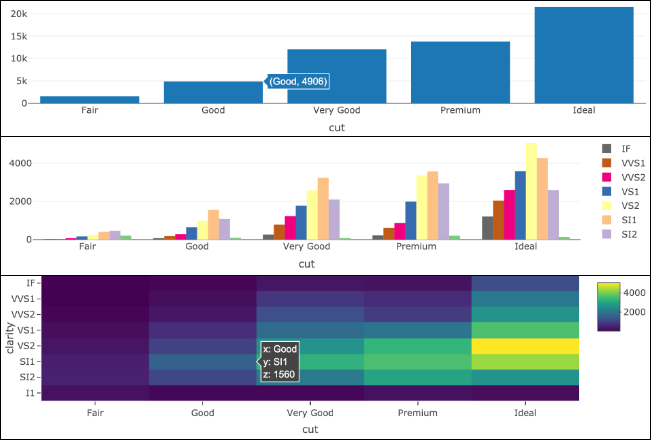
\includegraphics[width=\textwidth]{images/intro-defaults} 

}

\caption{Three examples of visualizing categorical data with \texttt{plot\_ly()}: (top) mapping \texttt{cut} to \texttt{x} yields a bar chart, (middle) mapping \texttt{cut} \& \texttt{clarity} to \texttt{x} \& \texttt{y} yields a heatmap, and (c) mapping \texttt{cut} \& \texttt{clarity} to \texttt{x} \& \texttt{color} yields a dodged bar chart.}\label{fig:intro-defaults}
\end{figure}

The \texttt{plot\_ly()} function has numerous arguments that are unique to the R package (e.g., \texttt{color}, \texttt{stroke}, \texttt{span}, \texttt{symbol}, \texttt{linetype}, etc) and make it easier to encode data variables (e.g., diamond clarity) as visual properties (e.g., color). By default, these arguments map values of a data variable to a visual range defined by the plural form of the argument. For example, in the bottom panel of \ref{fig:intro-defaults}, \texttt{color} is used to map each level of diamond clarity to a different color, then \texttt{colors} is used to specify the range of colors (which, in this case, the \texttt{"Accent"} color palette from the \textbf{RColorBrewer} package, but one can also supply custom color codes or a color palette function like \texttt{colorRamp()}). Figure \ref{fig:color-mapping} provides a visual diagram of how this particular mapping works, but the same sort of idea can be applied to other visual properties like size, shape, linetype, etc.

\begin{figure}

{\centering 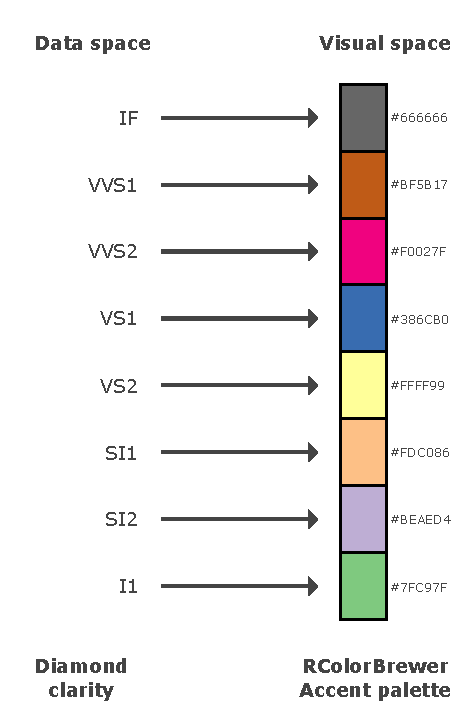
\includegraphics[width=0.45\linewidth]{images/color-mapping} 

}

\caption{Mapping data values to a visual color range.}\label{fig:color-mapping}
\end{figure}

Since these arguments map data values to a visual range by default, you will obtain unexpected results if you try to specify the visual range directly, as in the top portion of Figure \ref{fig:intro-range}. If you want to specify the visual range directly, use the \texttt{I()} function to declare this value to be taken `AsIs', as in the bottom portion of Figure \ref{fig:intro-range}. Throughout this book, you'll see lots of examples that leverage these arguments, especially in Chapter \ref{scatter-traces}. Another good resource to learn more about these arguments (especially their defaults) is the R documentation page available by entering \texttt{help(plot\_ly)} in your R console.

\index{plot\_ly()@\texttt{plot\_ly()}!I()@\texttt{I()}}

\begin{Shaded}
\begin{Highlighting}[]
\CommentTok{# doesn't produce black bars}
\KeywordTok{plot_ly}\NormalTok{(diamonds, }\DataTypeTok{x =} \OperatorTok{~}\NormalTok{cut, }\DataTypeTok{color =} \StringTok{"black"}\NormalTok{)}
\CommentTok{# produces red bars with black outline}
\KeywordTok{plot_ly}\NormalTok{(}
\NormalTok{  diamonds, }
  \DataTypeTok{x =} \OperatorTok{~}\NormalTok{cut, }
  \DataTypeTok{color =} \KeywordTok{I}\NormalTok{(}\StringTok{"red"}\NormalTok{), }
  \DataTypeTok{stroke =} \KeywordTok{I}\NormalTok{(}\StringTok{"black"}\NormalTok{), }
  \DataTypeTok{span =} \KeywordTok{I}\NormalTok{(}\DecValTok{2}\NormalTok{)}
\NormalTok{)}
\end{Highlighting}
\end{Shaded}

\begin{figure}

{\centering 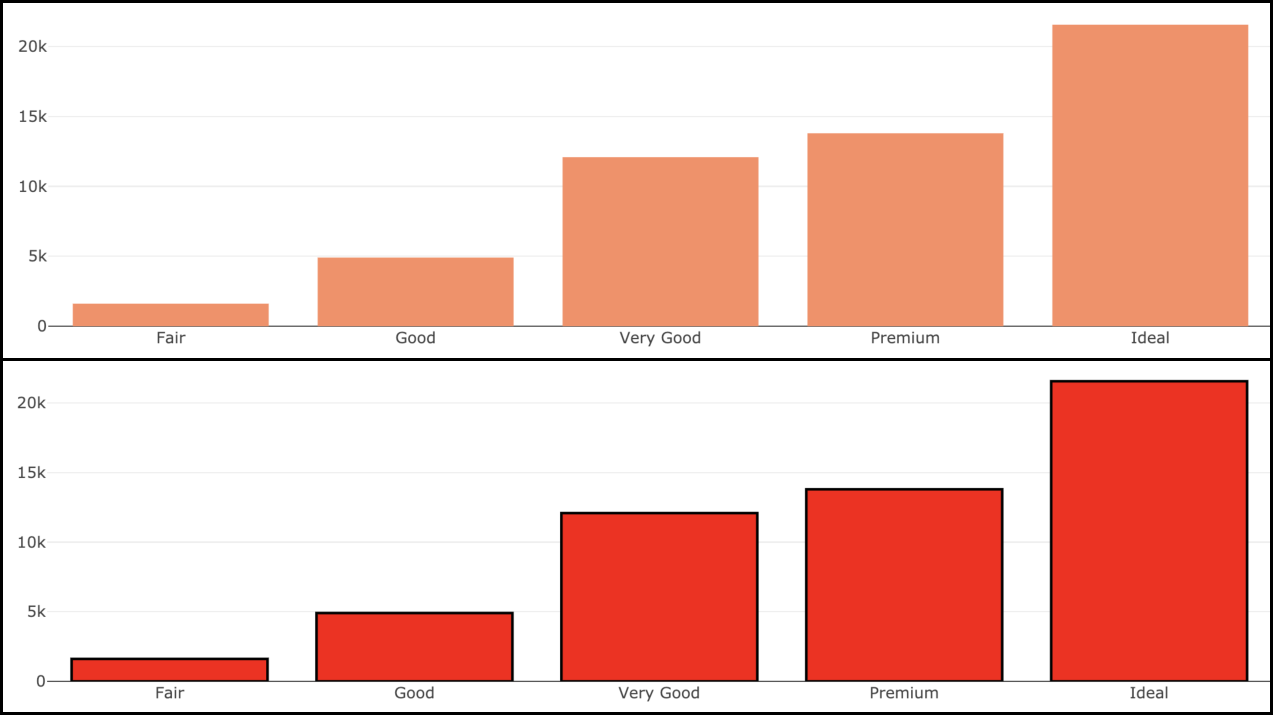
\includegraphics[width=\textwidth]{images/intro-range} 

}

\caption{Using \texttt{I()} to supply visual properties directly instead of mapping values to a visual range. In the top portion of this figure, the value \texttt{\textquotesingle{}black\textquotesingle{}} is being mapped to a visual range spanned by \texttt{colors} (which, for discrete data, defaults to \texttt{\textquotesingle{}Set2\textquotesingle{}}).}\label{fig:intro-range}
\end{figure}

The \textbf{plotly} package takes a purely functional approach to a layered grammar of graphics \citep{ggplot2-paper}.\footnote{If you aren't already familiar with the grammar of graphics or \textbf{ggplot2}, we recommend reading the Data Visualization chapter from the \emph{R for Data Science} book. \url{https://r4ds.had.co.nz/data-visualisation.html}} The purely functional part means, (almost) every function anticipates a \textbf{plotly} object as input to it's first argument and returns a modified version of that \textbf{plotly} object. Furthermore, that modification is completely determined by the input values to the function (i.e., it doesn't rely on any side-effects, unlike, for example, base R graphics). For a quick example, the \texttt{layout()} function anticipates a \textbf{plotly} object in it's first argument and it's other arguments add and/or modify various layout components of that object (e.g., the title):

\begin{Shaded}
\begin{Highlighting}[]
\KeywordTok{layout}\NormalTok{(}
  \KeywordTok{plot_ly}\NormalTok{(diamonds, }\DataTypeTok{x =} \OperatorTok{~}\NormalTok{cut),}
  \DataTypeTok{title =} \StringTok{"My beatiful histogram"}
\NormalTok{)}
\end{Highlighting}
\end{Shaded}

For more complex plots that modify a \textbf{plotly} graph many times over, code written in this way can become cumbersome to read. In particular, we have to search for the inner-most part of the R expression, then work outwards towards the end result. The \texttt{\%\textgreater{}\%} operator from the \textbf{magrittr} package allows us to re-arrange this code so that we can read the sequence of modifications from left-to-right rather than inside-out \citep{magrittr}. The \texttt{\%\textgreater{}\%} operator enable this by placing the object on the left-hand side of the \texttt{\%\textgreater{}\%} into the first argument of the function of the right-hand side.

\begin{Shaded}
\begin{Highlighting}[]
\NormalTok{diamonds }\OperatorTok
\StringTok{  }\KeywordTok{plot_ly}\NormalTok{(}\DataTypeTok{x =} \OperatorTok{~}\NormalTok{cut) }\OperatorTok
\StringTok{  }\KeywordTok{layout}\NormalTok{(}\DataTypeTok{title =} \StringTok{"My beatiful histogram"}\NormalTok{)}
\end{Highlighting}
\end{Shaded}

In addition to \texttt{layout()} for adding/modifying part(s) of the graph's layout, there are also a family of \texttt{add\_*()} functions (e.g., \texttt{add\_histogram()}, \texttt{add\_lines()}, etc) that define how to render data into geometric objects. Borrowing terminology from the layered grammar of graphics, these functions add a graphical layer to a plot. A \emph{layer} can be thought of as a group of graphical elements that can be sufficiently described using only 5 components: data, aesthetic mappings (e.g., assigning \texttt{clarity} to \texttt{color}), a geometric representation (e.g.~rectangles, circles, etc), statistical transformations (e.g., sum, mean, etc), and positional adjustments (e.g., dodge, stack, etc). If you're paying attention, you'll notice that in the examples thus far, we have not specified a layer! The layer has been added for us automatically by \texttt{plot\_ly()}. To be explicit about what \texttt{plot\_ly(diamonds,\ x\ =\ \textasciitilde{}cut)} generates, we should add a \texttt{add\_histogram()} layer:

\begin{Shaded}
\begin{Highlighting}[]
\NormalTok{diamonds }\OperatorTok
\StringTok{  }\KeywordTok{plot_ly}\NormalTok{() }\OperatorTok\StringTok{ }
\StringTok{  }\KeywordTok{add_histogram}\NormalTok{(}\DataTypeTok{x =} \OperatorTok{~}\NormalTok{cut)}
\end{Highlighting}
\end{Shaded}

As you'll learn more about in Chapter \ref{bars-histograms}, \textbf{plotly} has both \texttt{add\_histogram()} and \texttt{add\_bars()}. The difference is that \texttt{add\_histogram()} performs \emph{statistics} (i.e., a binning algorithm) dynamically in the web browser, whereas \texttt{add\_bars()} requires the bar heights to be pre-specified. That means, to replicate the last example with \texttt{add\_bars()}, the number of observations must be computed ahead-of-time.

\begin{Shaded}
\begin{Highlighting}[]
\NormalTok{diamonds }\OperatorTok
\StringTok{  }\NormalTok{dplyr}\OperatorTok{::}\KeywordTok{count}\NormalTok{(cut) }\OperatorTok
\StringTok{  }\KeywordTok{plot_ly}\NormalTok{() }\OperatorTok\StringTok{ }
\StringTok{  }\KeywordTok{add_bars}\NormalTok{(}\DataTypeTok{x =} \OperatorTok{~}\NormalTok{cut, }\DataTypeTok{y =} \OperatorTok{~}\NormalTok{n)}
\end{Highlighting}
\end{Shaded}

There are numerous other \texttt{add\_*()} functions that calculate statistics in the browser (e.g., \texttt{add\_histogram2d()}, \texttt{add\_contour()}, \texttt{add\_boxplot()}, etc), but most other functions aren't considered statistical. Making the distinction might not seem useful now, but they have their own respective trade-offs when it comes to speed and interactivity. Generally speaking, non-statistical layers will be faster and more responsive at run-time (since they require less computational work), whereas the statistical layers allow for more flexibility when it comes to client-side interactivity, as covered in Chapter \ref{client-side-linking}. Practically speaking, the difference in performance is often negligible -- the more common bottleneck occurs when attempting to render lots of graphical elements at a time (e.g., a scatterplot with a million points). In those scenarios, you likely want to render your plot in Canvas rather than SVG (the default) via \texttt{toWebGL()} -- for more information on improving performance, see Chapter \ref{performance}.

\index{plot\_ly()@\texttt{plot\_ly()}!Layered mappings}
\index{plot\_ly()@\texttt{plot\_ly()}!dplyr integration}

In many scenarios, it can be useful to combine multiple graphical layers into a single plot. In this case, it becomes useful to know a few things about \texttt{plot\_ly()}:

\begin{itemize}
\tightlist
\item
  Arguments specified in \texttt{plot\_ly()} are \emph{global}, meaning that any downstream \texttt{add\_*()} functions inherit these arguments (unless \texttt{inherit\ =\ FALSE}).
\item
  Data manipulation verbs from the \textbf{dplyr} package may be used to transform the \texttt{data} underlying a \textbf{plotly} object.\footnote{Technically speaking, these \textbf{dplyr} verbs are S3 generic functions that \textbf{plotly} has a defined a custom method for. In nearly every case, that custom method simply queries the data underlying the \textbf{plotly} object, applies the \textbf{dplyr} function, then adds the transformed data back into the resulting \textbf{plotly} object}
\end{itemize}

Using these two properties of \texttt{plot\_ly()}, Figure \ref{fig:intro-dplyr} demonstrates how we could leverage these properties of \texttt{plot\_ly()} to do the following:

\begin{enumerate}
\def\labelenumi{\arabic{enumi}.}
\tightlist
\item
  \emph{Globally} assign \texttt{cut} to \texttt{x}.
\item
  Add a histogram layer (inherits the \texttt{x} from \texttt{plot\_ly()}).
\item
  Use \textbf{dplyr} verbs to modify the \texttt{data} underlying the \textbf{plotly} object. Here we just count the number of diamonds in each \texttt{cut} category.
\item
  Add a layer of text using the summarized counts. Note that the global \texttt{x} mapping, as well as the other mappings local to this text layer (\texttt{text} and \texttt{y}), reflect data values from step 3.
\end{enumerate}

\begin{Shaded}
\begin{Highlighting}[]
\KeywordTok{library}\NormalTok{(dplyr)}

\NormalTok{diamonds }\OperatorTok
\StringTok{  }\KeywordTok{plot_ly}\NormalTok{(}\DataTypeTok{x =} \OperatorTok{~}\NormalTok{cut) }\OperatorTok\StringTok{ }
\StringTok{  }\KeywordTok{add_histogram}\NormalTok{() }\OperatorTok
\StringTok{  }\KeywordTok{group_by}\NormalTok{(cut) }\OperatorTok
\StringTok{  }\KeywordTok{summarise}\NormalTok{(}\DataTypeTok{n =} \KeywordTok{n}\NormalTok{()) }\OperatorTok
\StringTok{  }\KeywordTok{add_text}\NormalTok{(}
    \DataTypeTok{text =} \OperatorTok{~}\NormalTok{scales}\OperatorTok{::}\KeywordTok{comma}\NormalTok{(n), }\DataTypeTok{y =} \OperatorTok{~}\NormalTok{n, }
    \DataTypeTok{textposition =} \StringTok{"top middle"}\NormalTok{, }
    \DataTypeTok{cliponaxis =} \OtherTok{FALSE}
\NormalTok{  )}
\end{Highlighting}
\end{Shaded}

\begin{figure}

{\centering 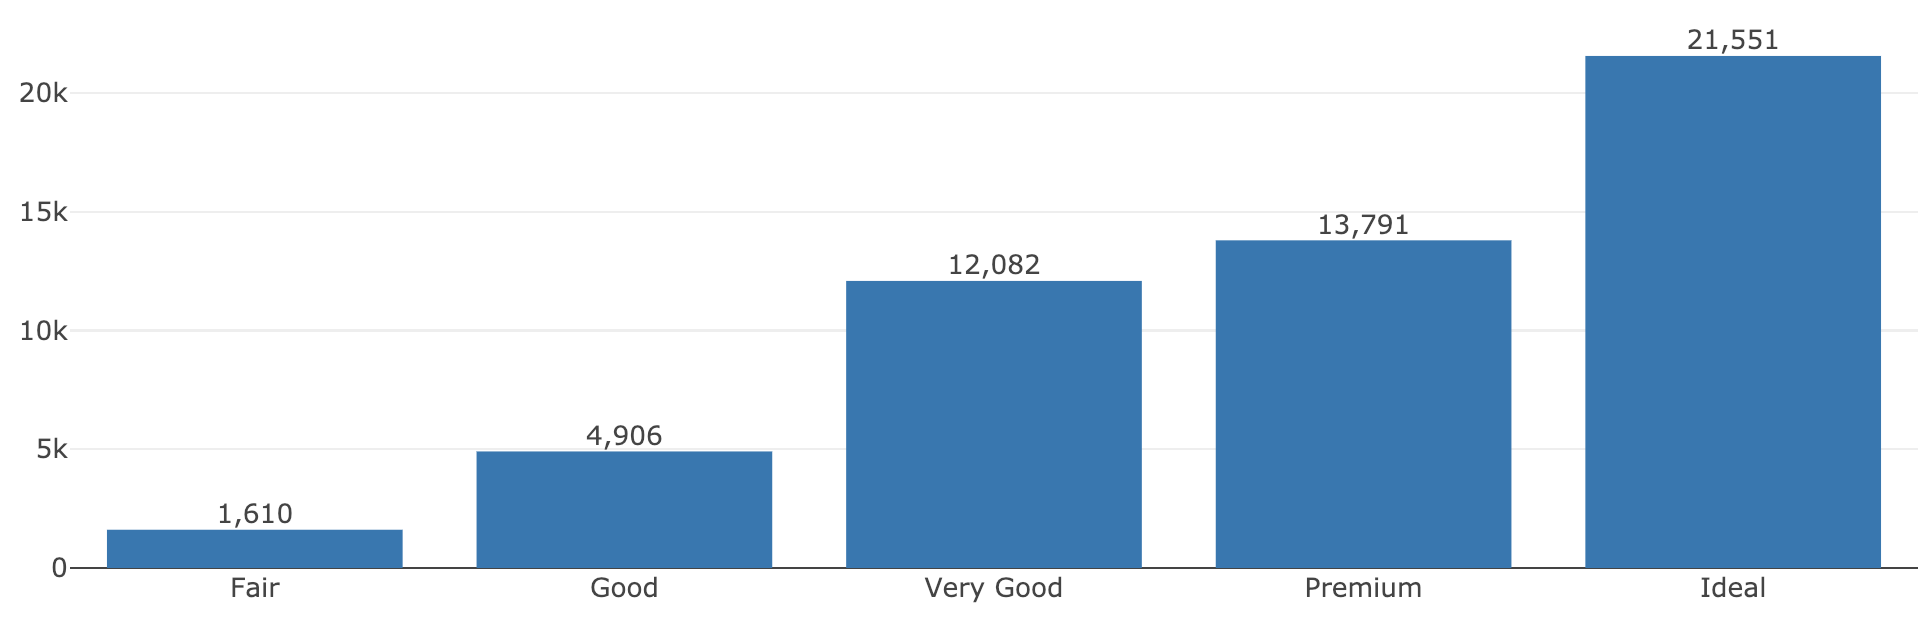
\includegraphics[width=\textwidth]{images/intro-dplyr} 

}

\caption{Using \texttt{add\_histogram()}, \texttt{add\_text()}, and \textbf{dplyr} verbs to compose a plot that leverages a raw form of the data (e.g., histogram) as well as a summarized version (e.g., text labels).}\label{fig:intro-dplyr}
\end{figure}

Before using multiple \texttt{add\_*()} in a single plot, make sure that you actually want to show those layers of information on the same set of axes. If it makes sense to display the information on the same axes, consider making multiple \textbf{plotly} objects and combining them into as grid-like layout using \texttt{subplot()}, as described in Chapter \ref{arranging-views}. Also, when using \textbf{dplyr} verbs to modify the \texttt{data} underlying the \textbf{plotly} object, you can use the \texttt{plotly\_data()} function to obtain the data at any point in time, which is primarily useful for debugging purposes (i.e., inspecting the data of a particular graphical layer).

\indexc{plotly\_data()}

\begin{Shaded}
\begin{Highlighting}[]
\NormalTok{diamonds }\OperatorTok
\StringTok{  }\KeywordTok{plot_ly}\NormalTok{(}\DataTypeTok{x =} \OperatorTok{~}\NormalTok{cut) }\OperatorTok\StringTok{ }
\StringTok{  }\KeywordTok{add_histogram}\NormalTok{() }\OperatorTok
\StringTok{  }\KeywordTok{group_by}\NormalTok{(cut) }\OperatorTok
\StringTok{  }\KeywordTok{summarise}\NormalTok{(}\DataTypeTok{n =} \KeywordTok{n}\NormalTok{()) }\OperatorTok\StringTok{ }
\StringTok{  }\KeywordTok{plotly_data}\NormalTok{()}
\CommentTok{#> # A tibble: 5 x 2}
\CommentTok{#>   cut           n}
\CommentTok{#>   <ord>     <int>}
\CommentTok{#> 1 Fair       1610}
\CommentTok{#> 2 Good       4906}
\CommentTok{#> 3 Very Good 12082}
\CommentTok{#> 4 Premium   13791}
\CommentTok{#> 5 Ideal     21551}
\end{Highlighting}
\end{Shaded}

This introduction to \texttt{plot\_ly()} has mainly focused on concepts unique to the R package \textbf{plotly} that are generally useful for creating most kinds of data views. The next section outlines how \textbf{plotly} generates plotly.js figures and how to inspect the underlying data structure that plotly.js uses to render the graph. Not only is this information useful for debugging, but it's also a nice way to learn how to work with plotly.js directly, which you may need to improve performance in \textbf{shiny} apps (Chapter \ref{proxies}) and/or for adding custom behavior with JavaScript (Chapter \ref{javascript}).

\hypertarget{intro-plotly-js}{%
\section{Intro to plotly.js}\label{intro-plotly-js}}

\indexc{plotly\_build()}

\index{plotly\_json()@\texttt{plotly\_json()}}
\index{plotly.js}

To recreate the plots in Figure \ref{fig:intro-defaults} using plotly.js \emph{directly}, it would take significantly more code and knowledge of plotly.js. That being said, learning how \textbf{plotly} generates the underlying plotly.js figure is a useful introduction to plotly.js itself, and knowledge of plotly.js becomes useful when you need more flexible control over \textbf{plotly}. As Figure \ref{fig:intro-printing} illustrates, when you print any \textbf{plotly} object, the \texttt{plotly\_build()} function is applied to that object, and that generates an R list which adheres to a syntax that plotly.js understands. This syntax is a JavaScript Object Notation (JSON) specification that plotly.js uses to represent, serialize, and render web graphics. A lot of documentation you'll find online about plotly (e.g., the online \href{https://plot.ly/r/reference/}{figure reference}) implicitly refers to this JSON specification, so it can helpful to know how to ``work backwards'' from that documentation (i.e., translate JSON into to R code). If you'd like to learn details about mapping between R and JSON, Chapter \ref{json} provides an introduction aimed at R programmers, and \citet{jsonlite} provides a cohesive overview of the \textbf{jsonlite} package, which is what \textbf{plotly} uses to map between R and JSON.

\begin{figure}

{\centering 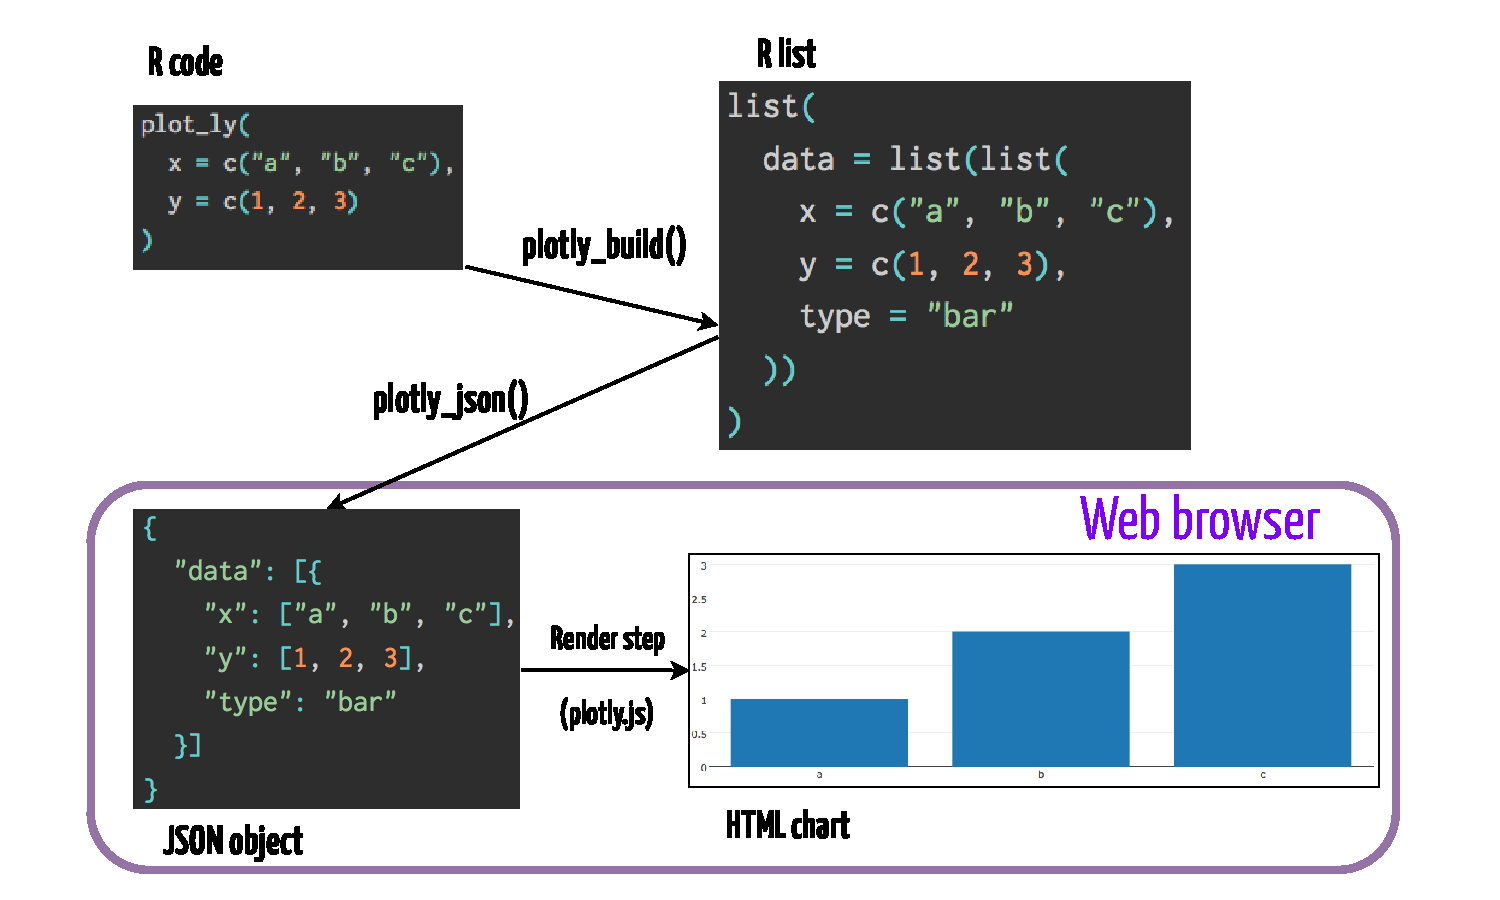
\includegraphics[width=\textwidth]{images/printing} 

}

\caption{A diagram of what happens when you print a \textbf{plotly} graph.}\label{fig:intro-printing}
\end{figure}

For illustration purposes, Figure \ref{fig:intro-printing} shows how this workflow applies to a simple bar graph (with values directly supplied instead of a data column name reference like Figure \ref{fig:intro-defaults}), but the same concept applies for any graph created via \textbf{plotly}. As the diagram suggests, both the \texttt{plotly\_build()} and \texttt{plotly\_json()} functions can be used to inspect the underlying data structure on both the R and JSON side of things. For example, Figure \ref{fig:intro-json} shows the \texttt{data} portion of the JSON created for the last graph in Figure \ref{fig:intro-json}.

\begin{Shaded}
\begin{Highlighting}[]
\NormalTok{p <-}\StringTok{ }\KeywordTok{plot_ly}\NormalTok{(diamonds, }\DataTypeTok{x =} \OperatorTok{~}\NormalTok{cut, }\DataTypeTok{color =} \OperatorTok{~}\NormalTok{clarity, }\DataTypeTok{colors =} \StringTok{"Accent"}\NormalTok{)}
\KeywordTok{plotly_json}\NormalTok{(p)}
\end{Highlighting}
\end{Shaded}

\begin{figure}

{\centering 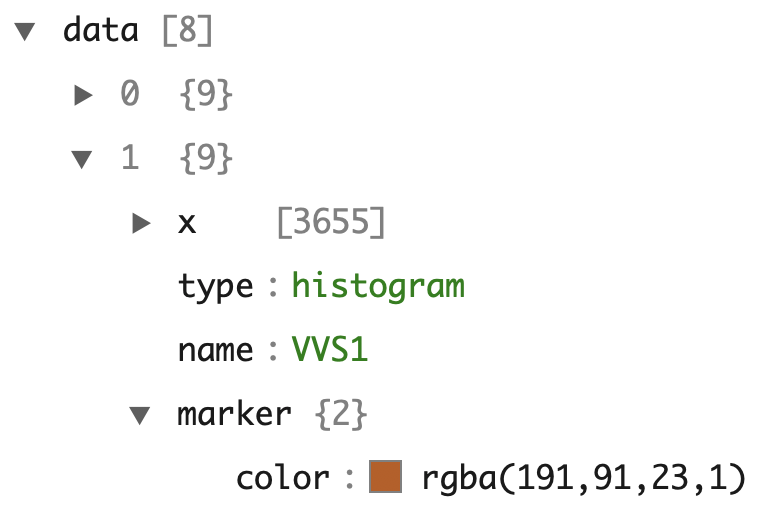
\includegraphics[width=0.7\linewidth]{images/intro-json} 

}

\caption{A portion of the JSON data behind the bottom plot of Figure \ref{fig:intro-defaults}. This dodged bar chart has 8 layers of data (i.e., 8 traces) -- one for each level of \texttt{clarity}.}\label{fig:intro-json}
\end{figure}

\index{Plotly figure!Definition}
\index{Plotly trace!Definition}

In plotly.js terminology, a \emph{figure} has two key components: \texttt{data} (aka, traces) and a \texttt{layout}. A \emph{trace} defines a mapping from data and visuals.\footnote{A trace is similar in concept to a layer (as defined in Section \ref{intro-plotly}, but it's not quite the same. In many cases, like the bottom panel of Figure \ref{fig:intro-defaults}, it makes sense to implement a single layer as multiple traces. This is due to the design of plotly.js and how traces are tied to legends and hover behavior.} Every trace has a \emph{type} (e.g., histogram, pie, scatter, etc) and the trace type determines what other attributes (i.e., visual and/or interactive properties, like \texttt{x}, \texttt{hoverinfo}, \texttt{name}) are available to control the trace mapping. That is, not every trace attribute is available to every trace type, but many attributes (e.g., the \texttt{name} of the trace) are available in every trace type and serve a similar purpose. From Figure \ref{fig:intro-json}, we can see that it takes multiple traces to generate the dodged bar chart, but instead of clicking through JSON viewer, sometimes it's easier to use \texttt{plotly\_build()} and compute on the plotly.js figure definition to verify certain things exist. Since \textbf{plotly} uses the \textbf{htmlwidgets} standard\footnote{The \textbf{htmlwidgets} package provides a foundation for other packages to implement R bindings to JavaScript libraries so that those bindings work in various contexts (e.g.~the R console, RStudio, inside \textbf{rmarkdown} documents, \textbf{shiny} apps, etc). For more info and examples, see the website \url{http://www.htmlwidgets.org}.}, the actual plotly.js figure definition appears under a list element named \texttt{x} \citep{htmlwidgets}.

\begin{Shaded}
\begin{Highlighting}[]
\CommentTok{# use plotly_build() to get at the plotly.js definition}
\CommentTok{# behind *any* plotly object}
\NormalTok{b <-}\StringTok{ }\KeywordTok{plotly_build}\NormalTok{(p)}

\CommentTok{# Confirm there 8 traces}
\KeywordTok{length}\NormalTok{(b}\OperatorTok{$}\NormalTok{x}\OperatorTok{$}\NormalTok{data)}
\CommentTok{#> [1] 8}

\CommentTok{# Extract the `name` of each trace. plotly.js uses `name` to }
\CommentTok{# populate legend entries and tooltips}
\NormalTok{purrr}\OperatorTok{::}\KeywordTok{map_chr}\NormalTok{(b}\OperatorTok{$}\NormalTok{x}\OperatorTok{$}\NormalTok{data, }\StringTok{"name"}\NormalTok{)}
\CommentTok{#> [1] "IF" "VVS1" "VVS2" "VS1" "VS2" "SI1" "SI2" "I1" }

\CommentTok{# Every trace has a type of histogram}
\KeywordTok{unique}\NormalTok{(purrr}\OperatorTok{::}\KeywordTok{map_chr}\NormalTok{(b}\OperatorTok{$}\NormalTok{x}\OperatorTok{$}\NormalTok{data, }\StringTok{"type"}\NormalTok{))}
\CommentTok{#> [1] "histogram"}
\end{Highlighting}
\end{Shaded}

Here we've learned that \textbf{plotly} creates 8 histogram traces to generate the dodged bar chart: one trace for each level of \texttt{clarity}.\footnote{Although the x-axis is discrete, plotly.js still considers this a histogram because it generates counts in the browser. Learn more about the difference between histograms and bar charts in Chapter \ref{bars-histograms}.} Why one trace per category? As illustrated in Figure \ref{fig:intro-show-hide}, there are two main reasons: to populate a tooltip and legend entry for each level of \texttt{clarity} level.

\begin{figure}

{\centering 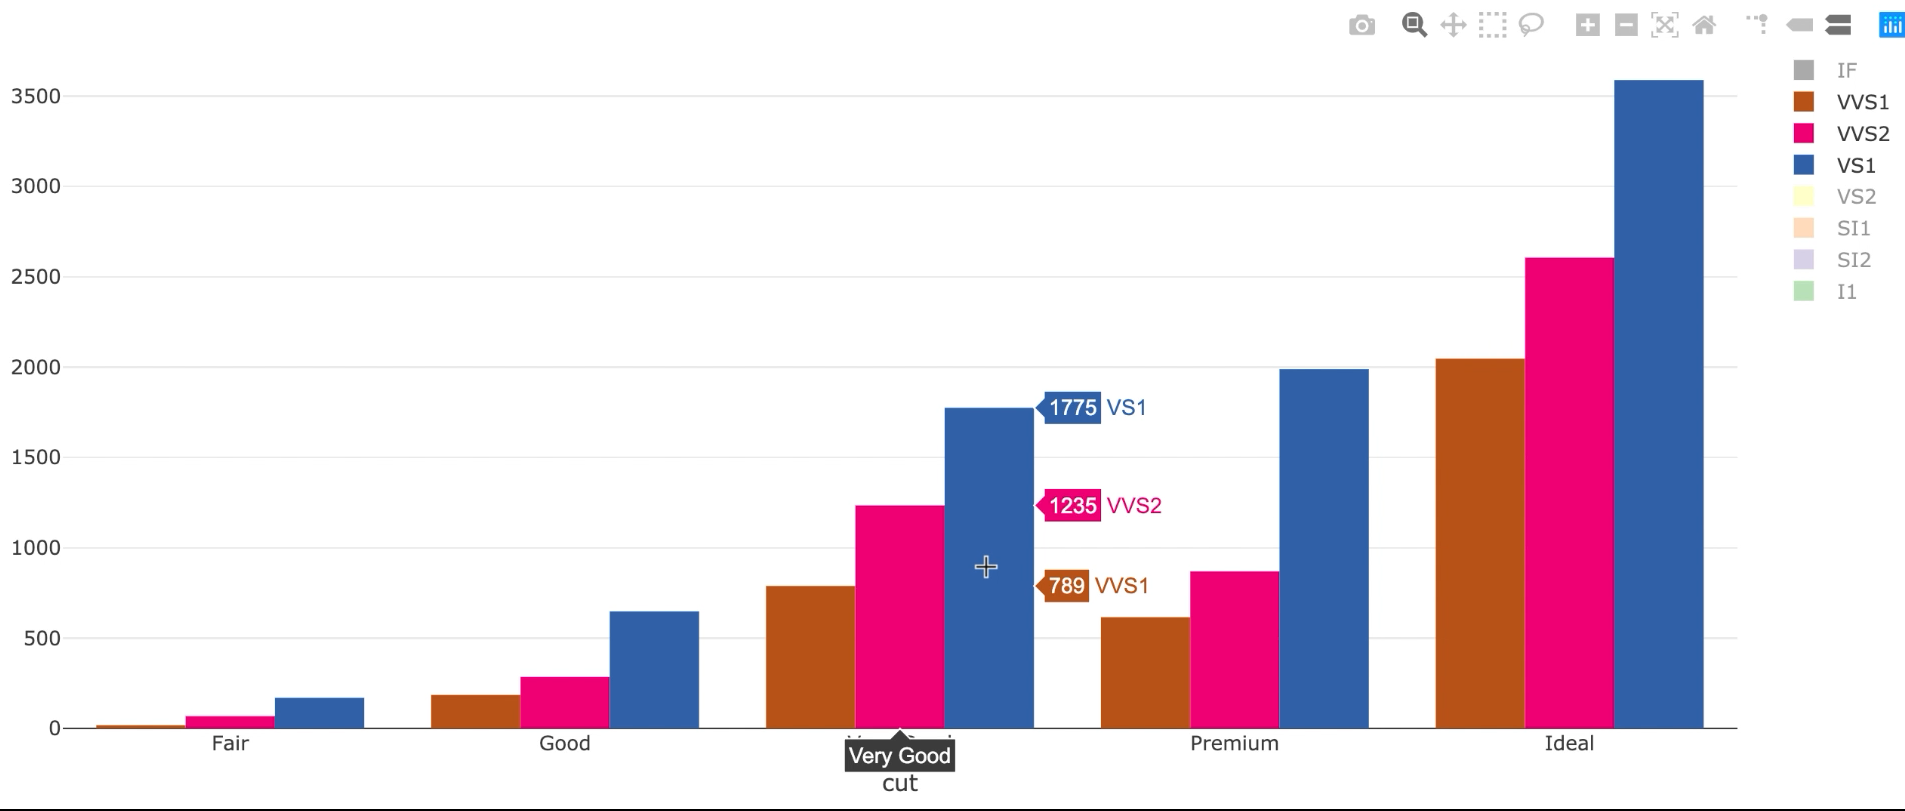
\includegraphics[width=\textwidth]{vimeo-images/315707813/final} 

}

\caption{Leveraging two interactive features that require one trace per level of \texttt{clarity}: (1) Using `Compare data on hover' mode to get counts for every level of \texttt{clarity} for a given level of \texttt{cut} and (2) Using the ability to hide/show clarity levels via their legend entries. For a video demonstration of the interactive, see \url{https://bit.ly/intro-show-hide-preview}. For the interactive, see \url{https://plotly-r.com/interactives/intro-show-hide.html}}\label{fig:intro-show-hide}
\end{figure}

If we investigated further, we'd notice that \texttt{color} and \texttt{colors} are not officially part of the plotly.js figure definition -- the \texttt{plotly\_build()} function has effectively transformed that information into a sensible plotly.js figure definition (e.g., \texttt{marker.color} contains the actual bar color codes). In fact, the \texttt{color} argument in \texttt{plot\_ly()} is just one example of an abstraction the R package has built on top of plotly.js to make it easier to map data values to visual attributes, and many of these are covered in Chapter \ref{scatter-traces}.

\hypertarget{intro-ggplotly}{%
\section{\texorpdfstring{Intro to \texttt{ggplotly()}}{Intro to ggplotly()}}\label{intro-ggplotly}}

\index{ggplotly()@\texttt{ggplotly()}}

The \texttt{ggplotly()} function from the \textbf{plotly} package has the ability to translate \textbf{ggplot2} to \textbf{plotly}. This functionality can be really helpful for quickly adding interactivity to your existing \textbf{ggplot2} workflow.\footnote{This section is not meant to teach you \textbf{ggplot2}, but rather to help point out when and why it might be preferable to \texttt{plot\_ly()}. If you're new to \textbf{ggplot2} and would like to learn it, see \ref{ggplot2}.} Moreover, even if you know \texttt{plot\_ly()} and plotly.js well, \texttt{ggplotly()} can still be desirable for creating visualizations that aren't necessarily straight-forward to achieve without it. To demonstrate, let's explore the relationship between \texttt{price} and other variables from the well-known \texttt{diamonds} dataset.

Hexagonal binning (i.e., \texttt{geom\_hex()}) is useful way to visualize a 2D density\footnote{See Section \ref{frequencies-2D} for approaches using \texttt{plot\_ly()}}, like the relationship between \texttt{price} and \texttt{carat} as shown in Figure \ref{fig:hexbin}. From Figure \ref{fig:hexbin}, we can see there is a strong positive linear relationship between the \emph{log} of carat and price. It also shows that for many, the carat is only rounded to a particular number (indicated by the light blue bands) and no diamonds are priced around \$1500. Making this plot interactive makes it easier to decode the hexagonal colors into the counts that they represent.

\index{ggplotly()@\texttt{ggplotly()}!ggplot2!geom\_hex()@\texttt{geom\_hex()}}

\begin{Shaded}
\begin{Highlighting}[]
\NormalTok{p <-}\StringTok{ }\KeywordTok{ggplot}\NormalTok{(diamonds, }\KeywordTok{aes}\NormalTok{(}\DataTypeTok{x =} \KeywordTok{log}\NormalTok{(carat), }\DataTypeTok{y =} \KeywordTok{log}\NormalTok{(price))) }\OperatorTok{+}\StringTok{ }
\StringTok{  }\KeywordTok{geom_hex}\NormalTok{(}\DataTypeTok{bins =} \DecValTok{100}\NormalTok{)}
\KeywordTok{ggplotly}\NormalTok{(p)}
\end{Highlighting}
\end{Shaded}

\begin{figure}

{\centering 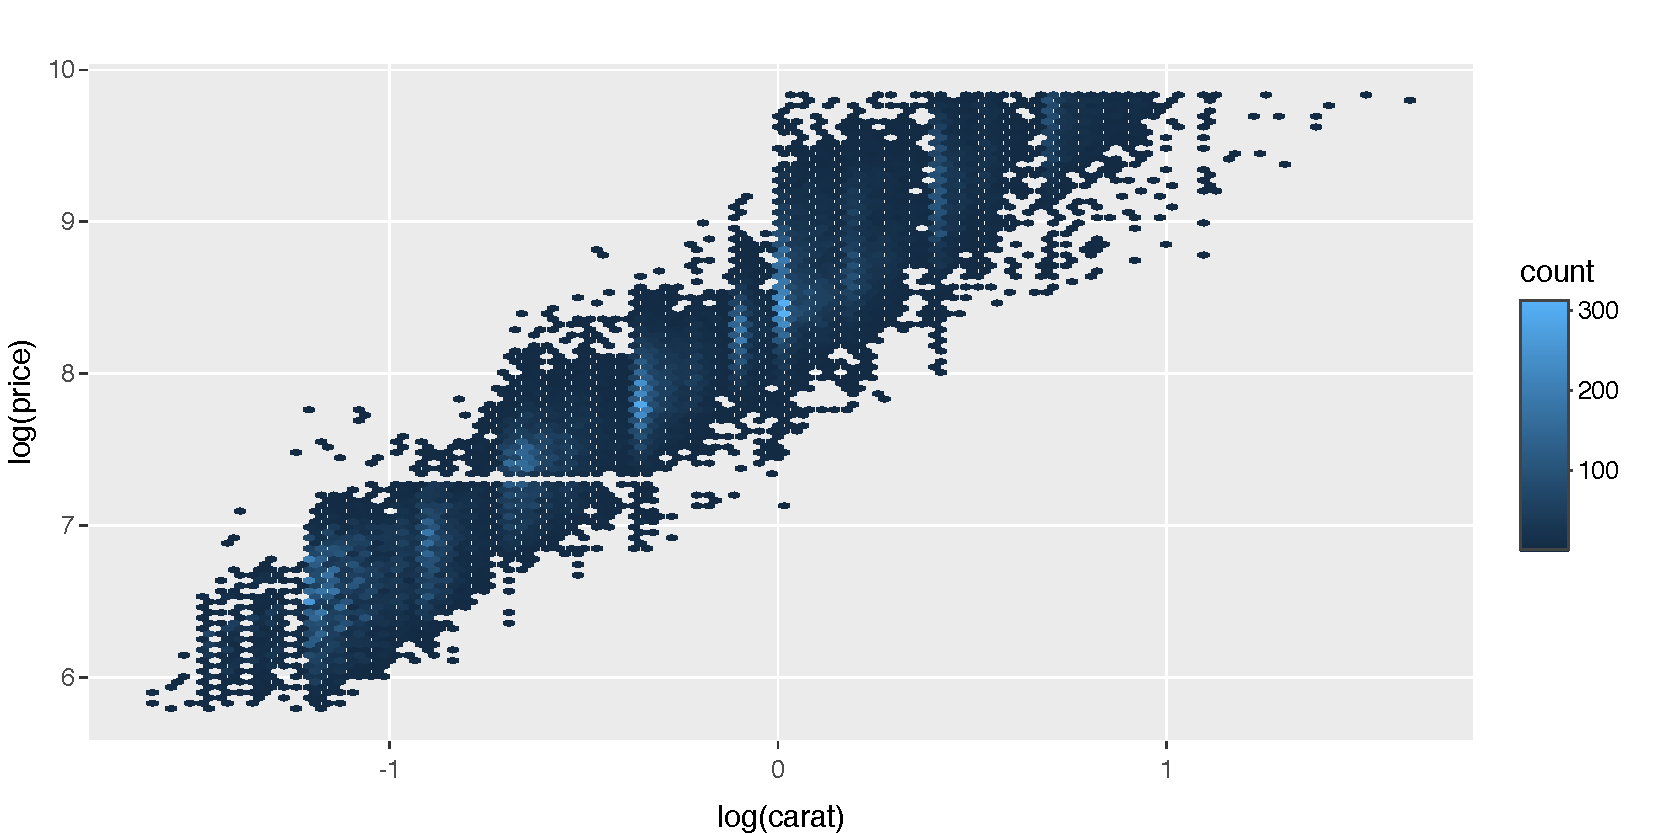
\includegraphics[width=\textwidth]{images/hexbin} 

}

\caption{A hexbin plot of diamond carat versus price.}\label{fig:hexbin}
\end{figure}

I often use \texttt{ggplotly()} over \texttt{plot\_ly()} to leverage \textbf{ggplot2}'s consistent and expressive interface for exploring statistical summaries across groups. For example, by including a discrete \texttt{color} variable (e.g., \texttt{cut}) with \texttt{geom\_freqpoly()}, you get a frequency polygon for each level of that variable. This ability to quickly generate visual encodings of statistical summaries across an arbitrary number of groups works for basically any geom (e.g.~\texttt{geom\_boxplot()}, \texttt{geom\_histogram()}, \texttt{geom\_density()}, etc) and is a key feature of \textbf{ggplot2}.

\index{ggplotly()@\texttt{ggplotly()}!ggplot2!geom\_freqpoly()@\texttt{geom\_freqpoly()}}

\begin{Shaded}
\begin{Highlighting}[]
\NormalTok{p <-}\StringTok{ }\KeywordTok{ggplot}\NormalTok{(diamonds, }\KeywordTok{aes}\NormalTok{(}\DataTypeTok{x =} \KeywordTok{log}\NormalTok{(price), }\DataTypeTok{color =}\NormalTok{ clarity)) }\OperatorTok{+}\StringTok{ }
\StringTok{    }\KeywordTok{geom_freqpoly}\NormalTok{()}
\KeywordTok{ggplotly}\NormalTok{(p)}
\end{Highlighting}
\end{Shaded}

\begin{figure}

{\centering 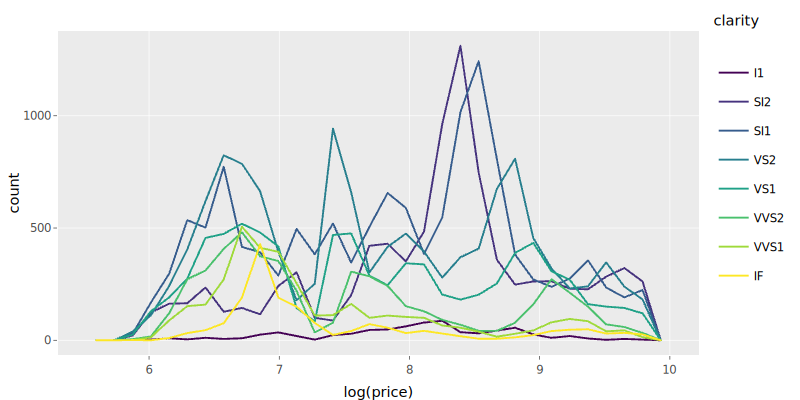
\includegraphics[width=\textwidth]{images/freqpoly} 

}

\caption{Frequency polygons of diamond price by diamond clarity. This visualization indicates there may be significant main effects.}\label{fig:freqpoly}
\end{figure}

Now, to see how \texttt{price} varies with both \texttt{cut} and \texttt{clarity}, we could repeat this same visualization for each level of \texttt{cut}. This is where \textbf{ggplot2}'s \texttt{facet\_wrap()} comes in handy. Moreover, to facilitate comparisons, we can have \texttt{geom\_freqpoly()} display relative rather than absolute frequencies. By making this plot interactive, we can more easily compare particular levels of clarity (as shown in Figure \ref{fig:freqpoly-facet}) by leveraging the legend filtering capabilities.

\index{ggplotly()@\texttt{ggplotly()}!ggplot2!facet\_wrap()@\texttt{facet\_wrap()}}

\begin{Shaded}
\begin{Highlighting}[]
\NormalTok{p <-}\StringTok{ }\KeywordTok{ggplot}\NormalTok{(diamonds, }\KeywordTok{aes}\NormalTok{(}\DataTypeTok{x =} \KeywordTok{log}\NormalTok{(price), }\DataTypeTok{color =}\NormalTok{ clarity)) }\OperatorTok{+}\StringTok{ }
\StringTok{    }\KeywordTok{geom_freqpoly}\NormalTok{(}\DataTypeTok{stat =} \StringTok{"density"}\NormalTok{) }\OperatorTok{+}\StringTok{ }
\StringTok{    }\KeywordTok{facet_wrap}\NormalTok{(}\OperatorTok{~}\NormalTok{cut)}
\KeywordTok{ggplotly}\NormalTok{(p)}
\end{Highlighting}
\end{Shaded}

\begin{figure}

{\centering 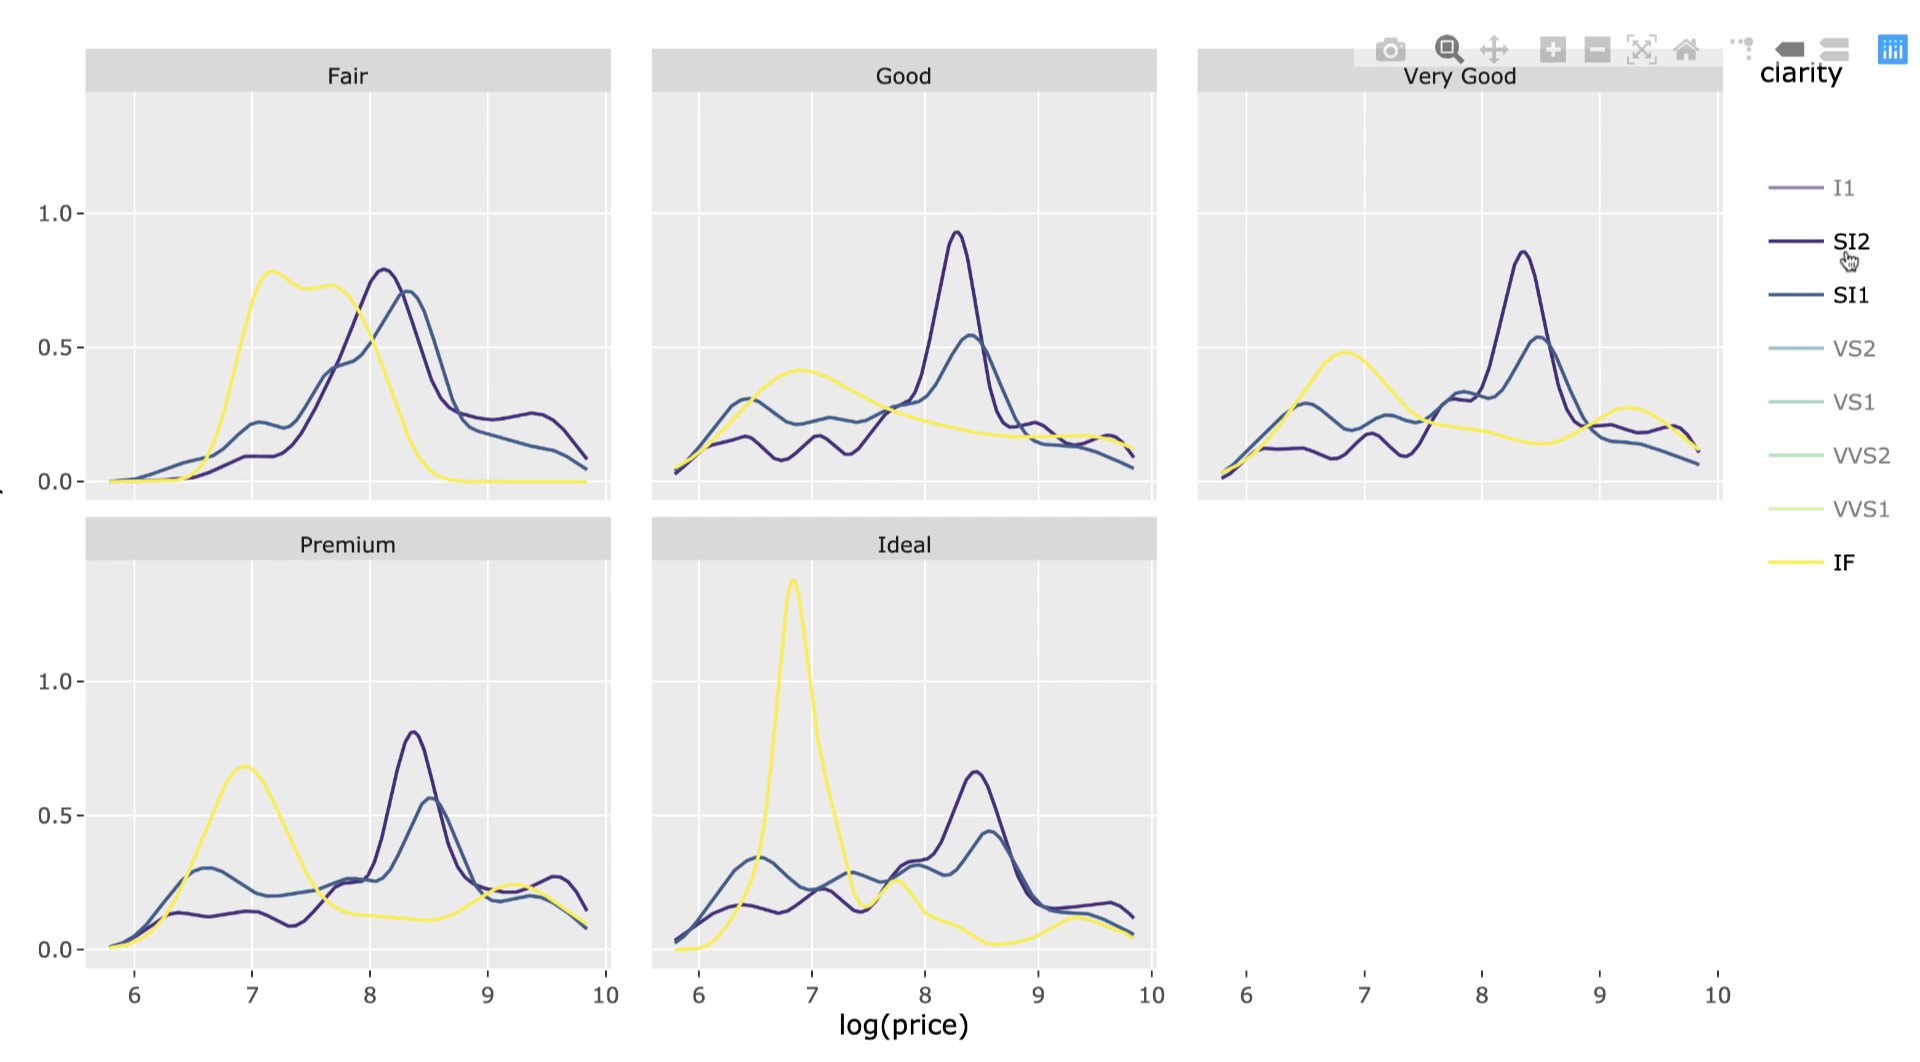
\includegraphics[width=\textwidth]{vimeo-images/322318131/final} 

}

\caption{Diamond price by clarity and cut. For a video demonstration of the interactive, see \url{https://bit.ly/freqpoly-facet}. For the interactive, see \url{https://plotly-r.com/interactives/freqpoly-facet.html}}\label{fig:freqpoly-facet}
\end{figure}

In addition to supporting most of the `core' \textbf{ggplot2} API, \texttt{ggplotly()} can automatically convert any \textbf{ggplot2} extension packages that return a `standard' \textbf{ggplot2} object. By standard, I mean that the object is comprised of `core' \textbf{ggplot2} data structures and not the result of custom geoms.\footnote{As discussed in \ref{custom-geoms}, \texttt{ggplotly()} can actually convert custom geoms as well, but each one requires a custom hook, and many custom geoms are not yet supported.} Some great examples of R packages that extend \textbf{ggplot2} using core data structures are \textbf{ggforce}, \textbf{naniar}, and \textbf{GGally} \citep{ggforce, naniar, GGally}.

Figure \ref{fig:geom-sina} demonstrates another way of visualizing the same information found in Figure \ref{fig:freqpoly-facet} using \texttt{geom\_sina()} from the \textbf{ggforce} package (instead of \texttt{geom\_freqpoly()}). This visualization jitters the raw data within the density for each group -- allowing us not only to see where the majority observations fall within a group, but also across all across all groups. By making this layer interactive, we can query individual points for more information and zoom into interesting regions. The second layer of Figure \ref{fig:geom-sina} uses \textbf{ggplot2}'s \texttt{stat\_summary()} to overlay a 95\% confidence interval estimated via a bootstrap algorithm via the \textbf{Hmisc} package \citep{Hmisc}.

\index{ggplotly()@\texttt{ggplotly()}!ggforce!geom\_sina()@\texttt{geom\_sina()}}
\index{ggplotly()@\texttt{ggplotly()}!ggplot2!stat\_summary()@\texttt{stat\_summary()}}
\index{toWebGL()@\texttt{toWebGL()}!ggplotly()@\texttt{ggplotly()}}

\begin{Shaded}
\begin{Highlighting}[]
\NormalTok{p <-}\StringTok{ }\KeywordTok{ggplot}\NormalTok{(diamonds, }\KeywordTok{aes}\NormalTok{(}\DataTypeTok{x=}\NormalTok{clarity, }\DataTypeTok{y=}\KeywordTok{log}\NormalTok{(price), }\DataTypeTok{color=}\NormalTok{clarity)) }\OperatorTok{+}
\StringTok{    }\NormalTok{ggforce}\OperatorTok{::}\KeywordTok{geom_sina}\NormalTok{(}\DataTypeTok{alpha =} \FloatTok{0.1}\NormalTok{) }\OperatorTok{+}\StringTok{ }
\StringTok{    }\KeywordTok{stat_summary}\NormalTok{(}\DataTypeTok{fun.data =} \StringTok{"mean_cl_boot"}\NormalTok{, }\DataTypeTok{color =} \StringTok{"black"}\NormalTok{) }\OperatorTok{+}
\StringTok{    }\KeywordTok{facet_wrap}\NormalTok{(}\OperatorTok{~}\NormalTok{cut)}

\CommentTok{# WebGL is a lot more efficient at rendering lots of points}
\KeywordTok{toWebGL}\NormalTok{(}\KeywordTok{ggplotly}\NormalTok{(p))}
\end{Highlighting}
\end{Shaded}

\begin{figure}

{\centering 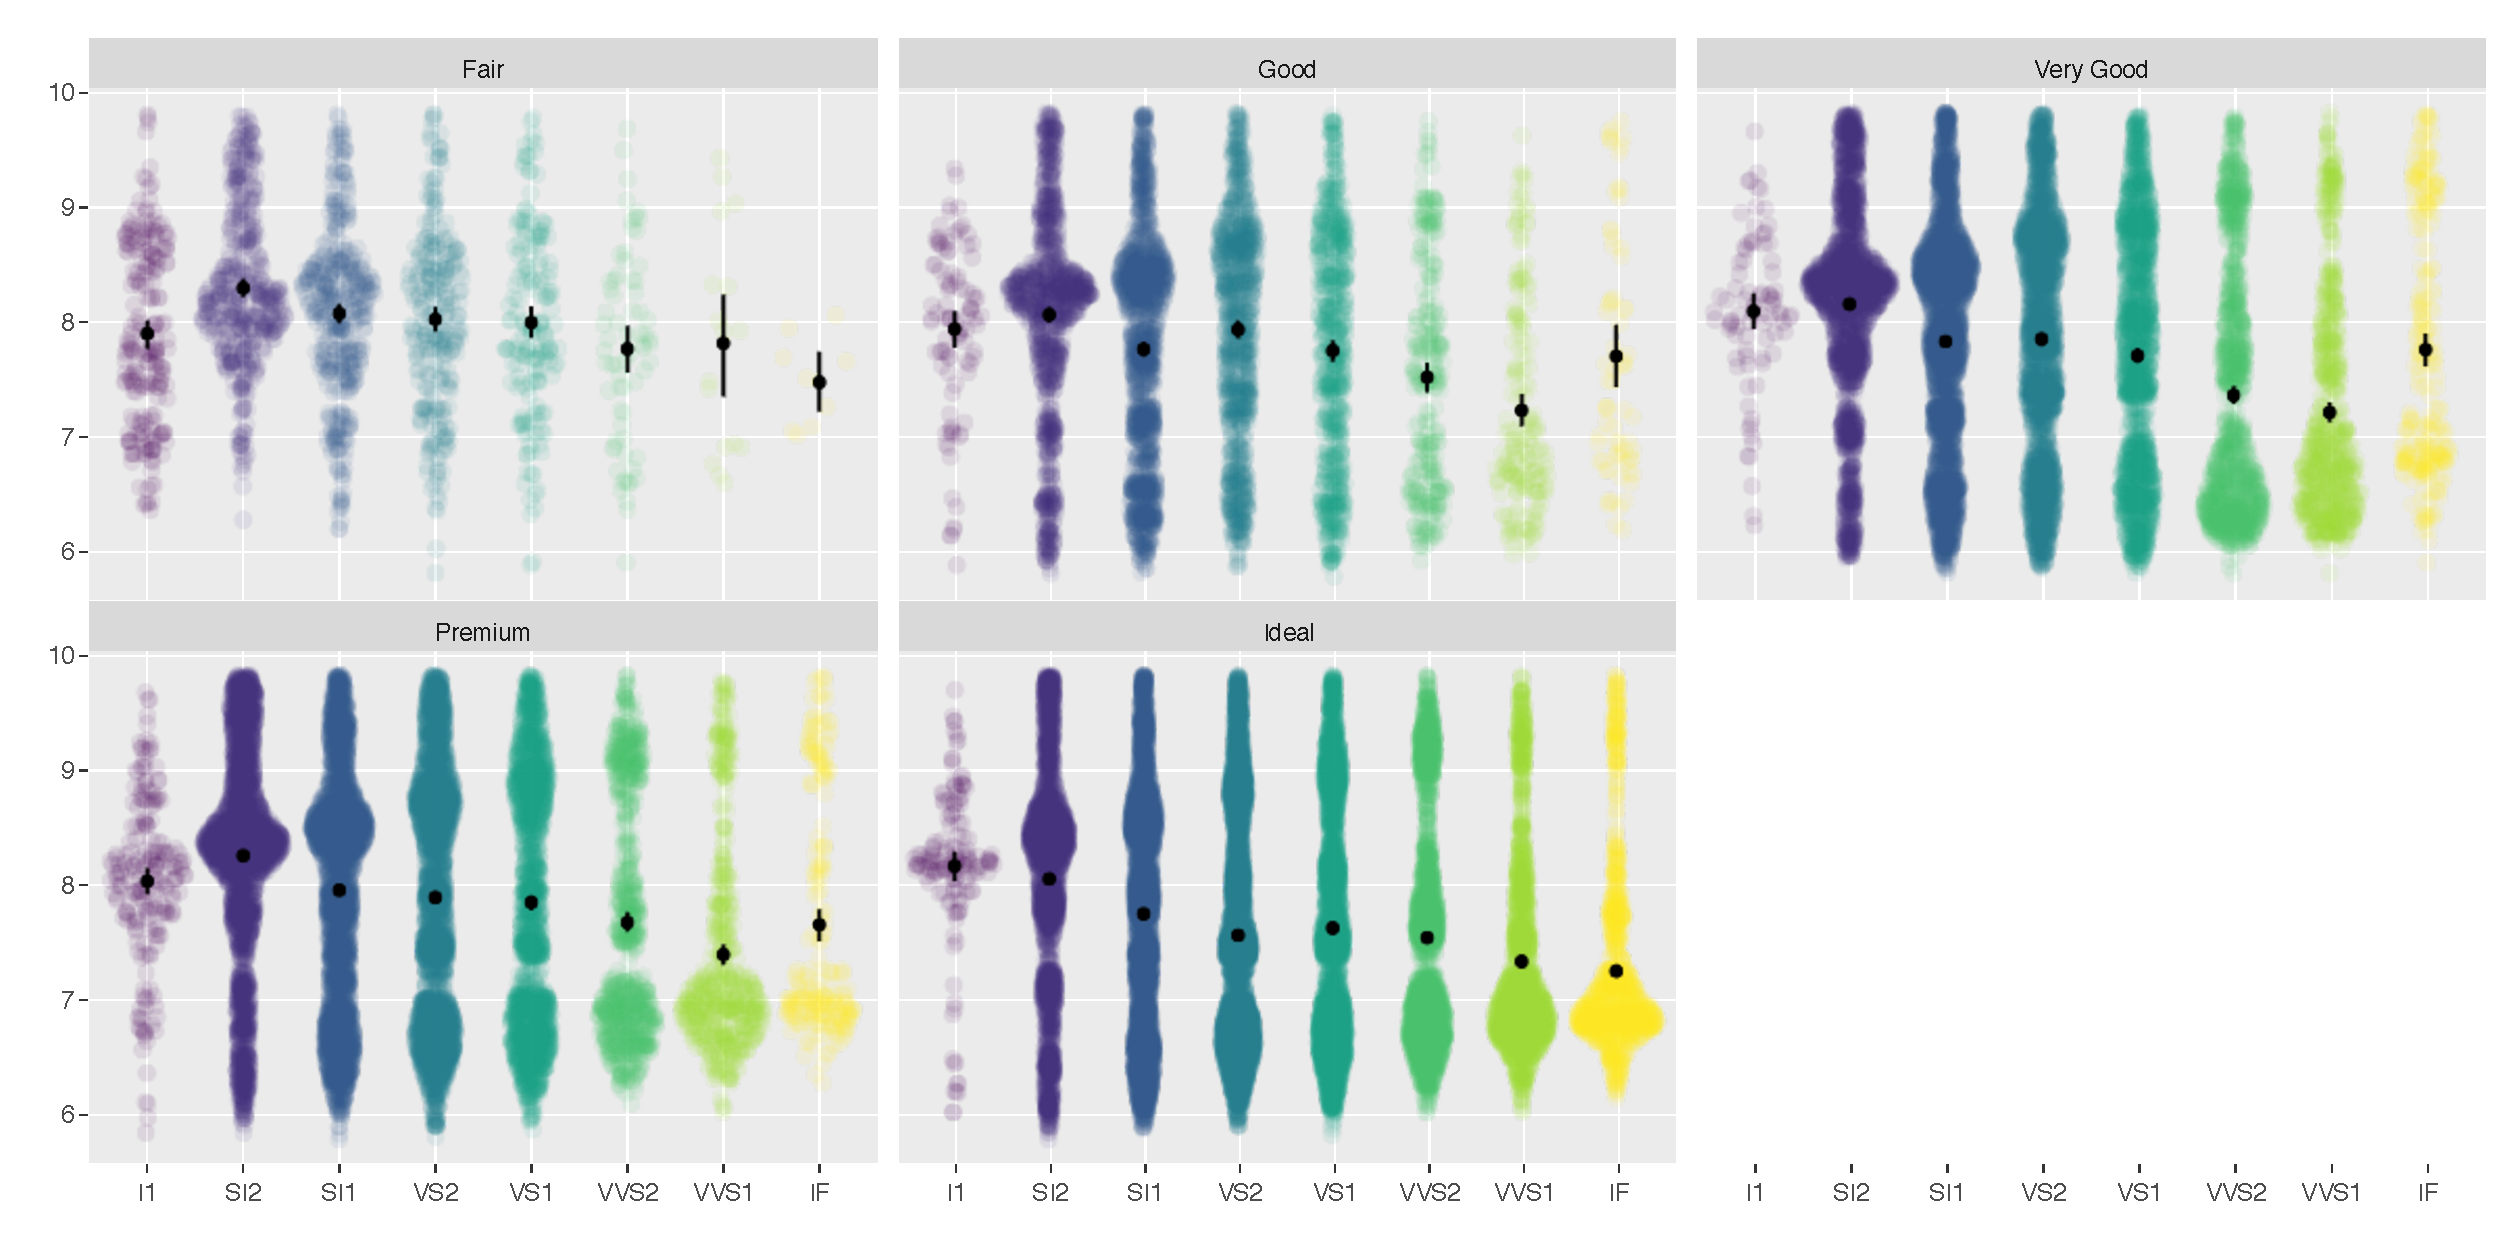
\includegraphics[width=\textwidth]{images/geom-sina} 

}

\caption{A sina plot of diamond price by clarity and cut.}\label{fig:geom-sina}
\end{figure}

As noted by \citet{r4ds}, it's surprising that the diamond price would decline with an increase of diamond clarity. As it turns out, if we account for the carat of the diamond, then see that better diamond clarity does indeed lead to a higher diamond price, as shown in Figure \ref{fig:geom-sina-resid}. Seeing such a strong pattern in the residuals of simple linear model of carat vs price indicates that our model could be greatly improved by adding \texttt{clarity} as a predictor of \texttt{price}.

\begin{Shaded}
\begin{Highlighting}[]
\NormalTok{m <-}\StringTok{ }\KeywordTok{lm}\NormalTok{(}\KeywordTok{log}\NormalTok{(price) }\OperatorTok{~}\StringTok{ }\KeywordTok{log}\NormalTok{(carat), }\DataTypeTok{data =}\NormalTok{ diamonds)}
\NormalTok{diamonds <-}\StringTok{ }\NormalTok{modelr}\OperatorTok{::}\KeywordTok{add_residuals}\NormalTok{(diamonds, m)}
\NormalTok{p <-}\StringTok{ }\KeywordTok{ggplot}\NormalTok{(diamonds, }\KeywordTok{aes}\NormalTok{(}\DataTypeTok{x =}\NormalTok{ clarity, }\DataTypeTok{y =}\NormalTok{ resid, }\DataTypeTok{color =}\NormalTok{ clarity)) }\OperatorTok{+}
\StringTok{    }\NormalTok{ggforce}\OperatorTok{::}\KeywordTok{geom_sina}\NormalTok{(}\DataTypeTok{alpha =} \FloatTok{0.1}\NormalTok{) }\OperatorTok{+}\StringTok{ }
\StringTok{    }\KeywordTok{stat_summary}\NormalTok{(}\DataTypeTok{fun.data =} \StringTok{"mean_cl_boot"}\NormalTok{, }\DataTypeTok{color =} \StringTok{"black"}\NormalTok{) }\OperatorTok{+}
\StringTok{    }\KeywordTok{facet_wrap}\NormalTok{(}\OperatorTok{~}\NormalTok{cut)}
\KeywordTok{toWebGL}\NormalTok{(}\KeywordTok{ggplotly}\NormalTok{(p))}
\end{Highlighting}
\end{Shaded}

\begin{figure}

{\centering 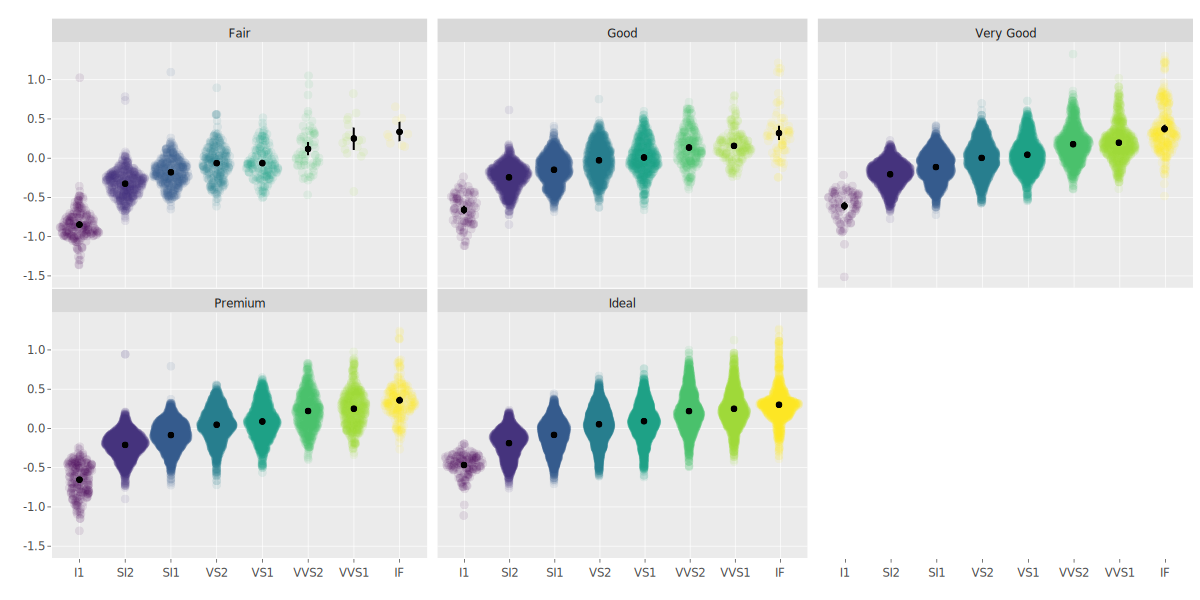
\includegraphics[width=\textwidth]{images/geom-sina-resid} 

}

\caption{A sina plot of diamond price by clarity and cut, after accounting for carat.}\label{fig:geom-sina-resid}
\end{figure}

\index{ggplotly()@\texttt{ggplotly()}!GGally!ggcoef()@\texttt{ggcoef()}}

As discussed in Chapter \ref{ggally-ggnostic}, the \textbf{GGally} package provides a convenient interface for making similar types of model diagnostic visualizations via the \texttt{ggnostic()} function. It also provides a convenience function for visualizing the coefficient estimates and their standard errors via the \texttt{ggcoef()} function. Figure \ref{fig:ggally} shows how injecting interactivity into this plot allows us to query exact values and zoom in on the most interesting regions.

\begin{Shaded}
\begin{Highlighting}[]
\KeywordTok{library}\NormalTok{(GGally)}
\NormalTok{m <-}\StringTok{ }\KeywordTok{lm}\NormalTok{(}\KeywordTok{log}\NormalTok{(price) }\OperatorTok{~}\StringTok{ }\KeywordTok{log}\NormalTok{(carat) }\OperatorTok{+}\StringTok{ }\NormalTok{cut, }\DataTypeTok{data =}\NormalTok{ diamonds)}
\NormalTok{gg <-}\StringTok{ }\KeywordTok{ggcoef}\NormalTok{(m)}
\CommentTok{# dynamicTicks means generate new axis ticks on zoom}
\KeywordTok{ggplotly}\NormalTok{(gg, }\DataTypeTok{dynamicTicks =} \OtherTok{TRUE}\NormalTok{)}
\end{Highlighting}
\end{Shaded}

\begin{figure}

{\centering 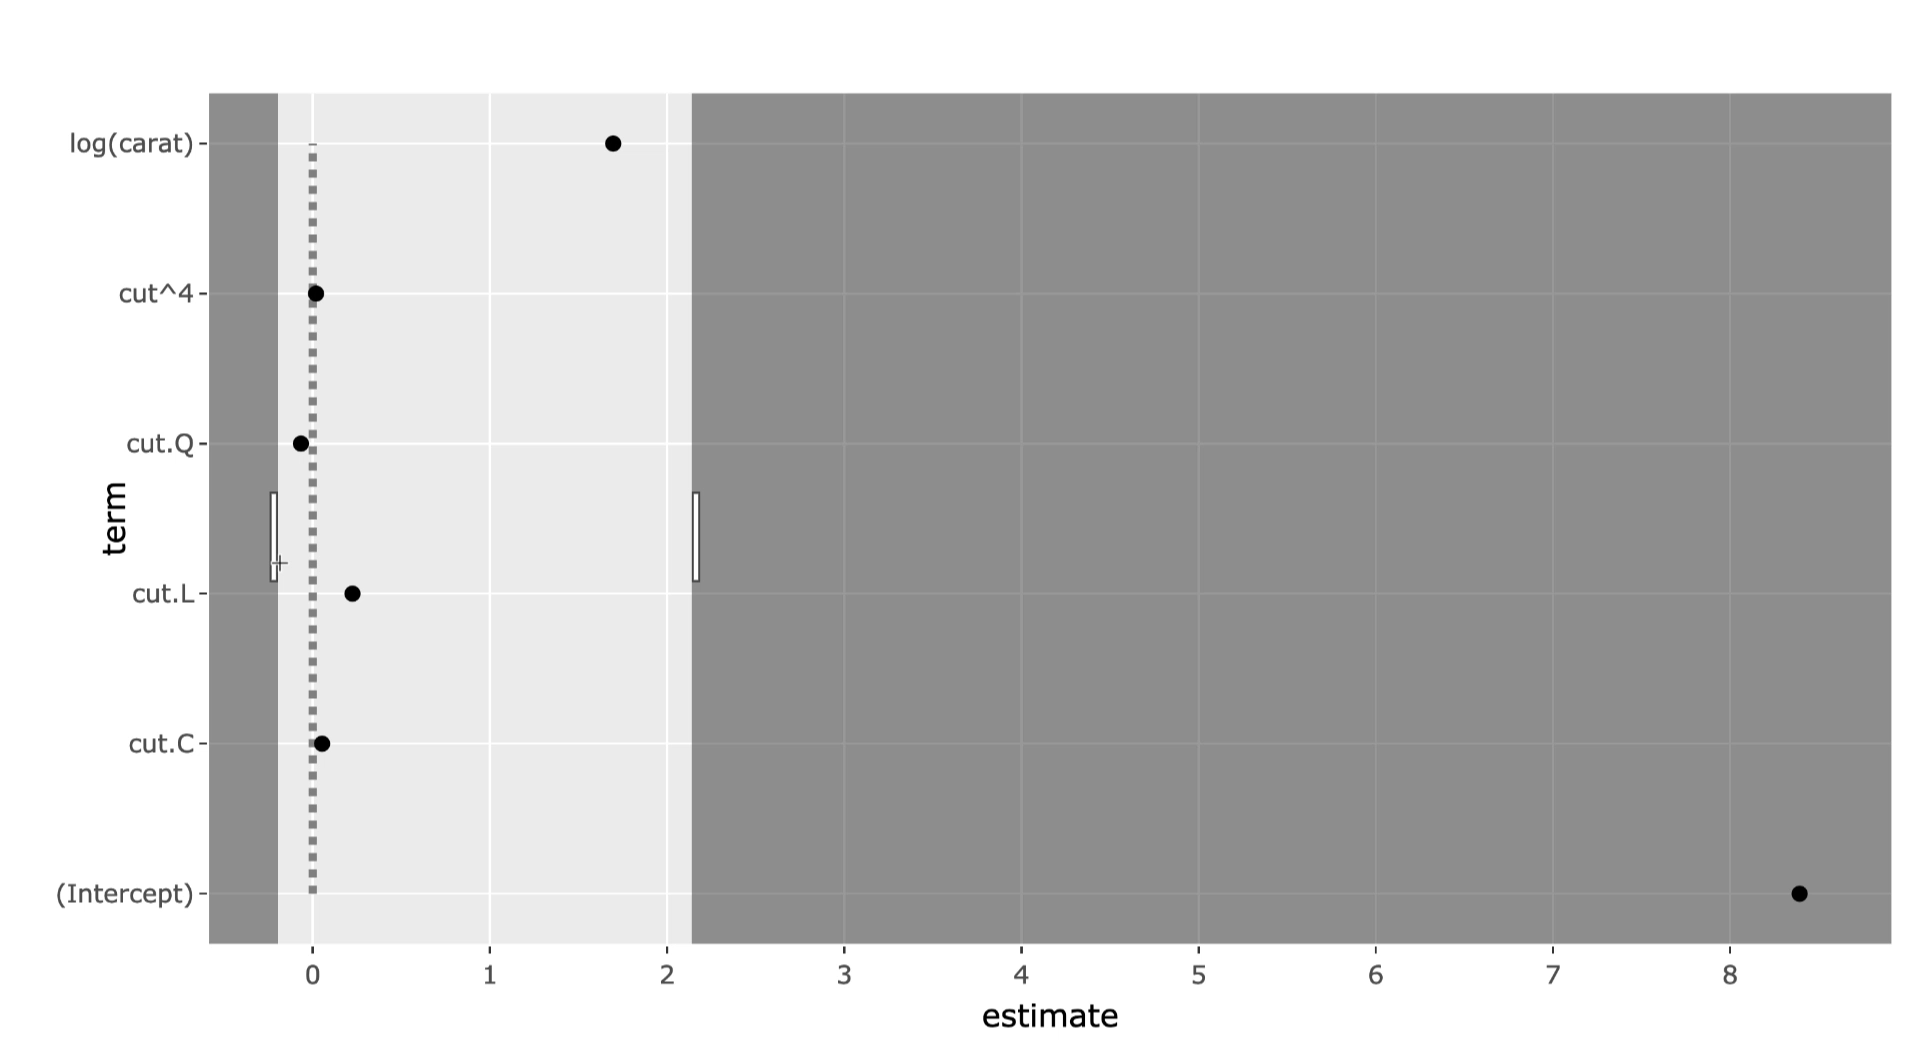
\includegraphics[width=\textwidth]{vimeo-images/322362701/final} 

}

\caption{Zooming in on a coefficient plot generated from the \texttt{ggcoef()} function from the \textbf{GGally} package. For a video demonstration of the interactive, see \url{https://bit.ly/GGally}. For the interactive, see \url{https://plotly-r.com/interactives/ggally.html}}\label{fig:ggally}
\end{figure}

Although the \texttt{diamonds} dataset does not contain any missing values, it's a very common problem in real data analysis problems. The \textbf{naniar} package provides a suite of computational and visual resources for working with and revealing structure in missing values. All the \textbf{ggplot2} based visualizations return an object that can be converted by \texttt{ggplotly()}. Moreover, \textbf{naniar} provides a custom geom, \texttt{geom\_miss\_point()}, that can be useful for visualizing missingness structure. Figure \ref{fig:naniar} demonstrates this by introducing fake missing values to the diamond price.

\index{ggplotly()@\texttt{ggplotly()}!naniar!geom\_miss\_point()@\texttt{geom\_miss\_point()}}

\begin{Shaded}
\begin{Highlighting}[]
\KeywordTok{library}\NormalTok{(naniar)}
\CommentTok{# fake some missing data}
\NormalTok{diamonds}\OperatorTok{$}\NormalTok{price_miss <-}\StringTok{ }\KeywordTok{ifelse}\NormalTok{(diamonds}\OperatorTok{$}\NormalTok{depth}\OperatorTok{>}\DecValTok{60}\NormalTok{, diamonds}\OperatorTok{$}\NormalTok{price, }\OtherTok{NA}\NormalTok{)}
\NormalTok{p <-}\StringTok{ }\KeywordTok{ggplot}\NormalTok{(diamonds, }\KeywordTok{aes}\NormalTok{(}\DataTypeTok{x =}\NormalTok{ clarity, }\DataTypeTok{y =} \KeywordTok{log}\NormalTok{(price_miss))) }\OperatorTok{+}
\StringTok{    }\KeywordTok{geom_miss_point}\NormalTok{(}\DataTypeTok{alpha =} \FloatTok{0.1}\NormalTok{) }\OperatorTok{+}\StringTok{ }
\StringTok{    }\KeywordTok{stat_summary}\NormalTok{(}\DataTypeTok{fun.data =} \StringTok{"mean_cl_boot"}\NormalTok{, }\DataTypeTok{colour =} \StringTok{"black"}\NormalTok{) }\OperatorTok{+}
\StringTok{    }\KeywordTok{facet_wrap}\NormalTok{(}\OperatorTok{~}\NormalTok{cut)}
\KeywordTok{toWebGL}\NormalTok{(}\KeywordTok{ggplotly}\NormalTok{(p))}
\end{Highlighting}
\end{Shaded}

\begin{figure}

{\centering 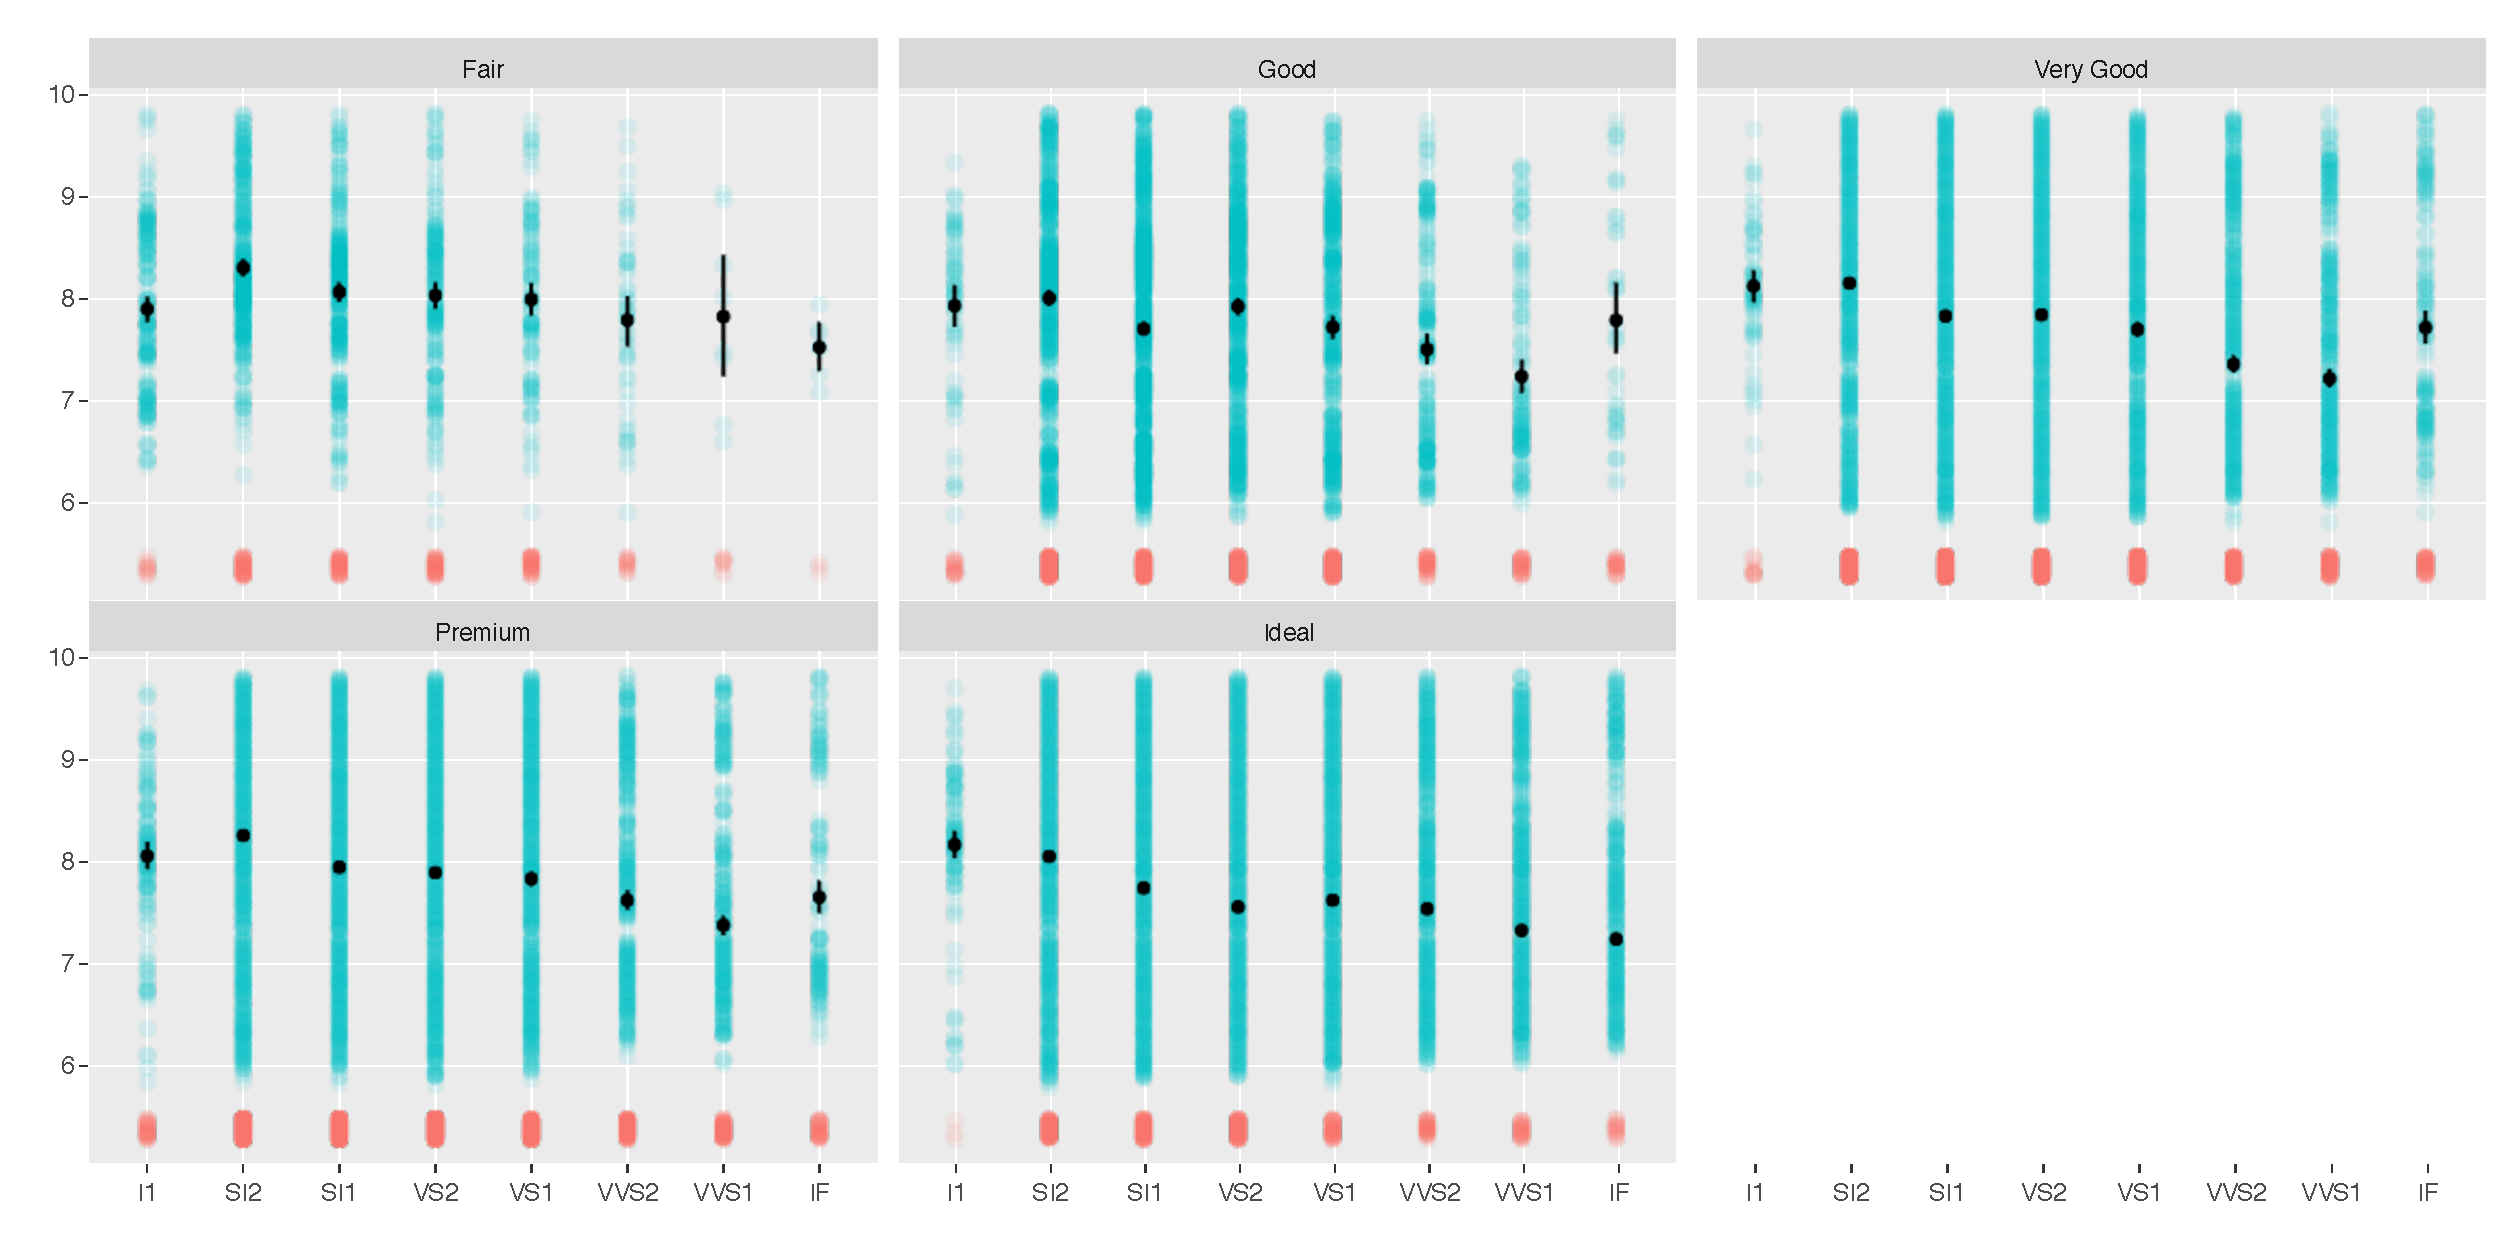
\includegraphics[width=\textwidth]{images/naniar} 

}

\caption{Using the \texttt{geom\_miss\_point()} function from the \textbf{naniar} package to visualize missing values in relation to non-missing values. Missing values are shown in red.}\label{fig:naniar}
\end{figure}

In short, the \textbf{ggplot2} ecosystem provides a world-class exploratory visualization toolkit, and having the ability to quickly insert interactivity such as hover, zoom, and filter via \texttt{ggplotly()} makes it even more powerful for exploratory analysis. In this introduction to \texttt{ggplotly()}, we've only seen relatively simple techniques that come for free out-of-the-box, but the true power of interactive graphics lies in linking multiple views. In that part of the book, you can find lots of examples of linking multiple (\texttt{ggplotly()} \& \texttt{plot\_ly()}) graphs purely client-side as well as with \textbf{shiny}.

It's also worth mentioning that \texttt{ggplotly()} conversions are not always perfect and \textbf{ggplot2} doesn't provide an API for interactive features, so sometimes it's desirable to modify the return values of \texttt{ggplotly()}. Chapter \ref{improving-ggplotly} talks generally about modifying the data structure underlying \texttt{ggplotly()} (which, by the way, uses the same a plotly.js figure definition as discussed in Section \ref{intro-plotly-js}). Moreover, Chapter \ref{tooltip-text-ggplotly} outlines various ways to customize the tooltip that \texttt{ggplotly()} produces.

\hypertarget{scatter-traces}{%
\chapter{Scattered foundations}\label{scatter-traces}}

\index{Scatter trace type}

As we learned in Section \ref{intro-plotly-js}, a plotly.js figure contains one (or more) trace(s), and every trace has a type. The trace type scatter is great for drawing low-level geometries (e.g., points, lines, text, and polygons) and provides the foundation for many \texttt{add\_*()} functions (e.g., \texttt{add\_markers()}, \texttt{add\_lines()}, \texttt{add\_paths()}, \texttt{add\_segments()}, \texttt{add\_ribbons()}, \texttt{add\_area()}, and \texttt{add\_polygons()}) as well as many \texttt{ggplotly()} charts. These scatter-based layers provide a more convenient interface to special cases of the scatter trace by doing a bit of data wrangling and transformation under-the-hood before mapping to scatter trace(s). For a simple example, \texttt{add\_lines()} ensures lines are drawn according to the ordering of \texttt{x}, which is desirable for a time series plotting. This behavior is subtly different than \texttt{add\_paths()} which uses row ordering instead.

\index{add\_trace()@\texttt{add\_trace()}!add\_paths()@\texttt{add\_paths()}}
\index{add\_trace()@\texttt{add\_trace()}!add\_lines()@\texttt{add\_lines()}}

\begin{Shaded}
\begin{Highlighting}[]
\KeywordTok{library}\NormalTok{(plotly)}
\KeywordTok{data}\NormalTok{(economics, }\DataTypeTok{package =} \StringTok{"ggplot2"}\NormalTok{)}

\CommentTok{# sort economics by psavert, just to }
\CommentTok{# show difference between paths and lines}
\NormalTok{p <-}\StringTok{ }\NormalTok{economics }\OperatorTok
\StringTok{  }\KeywordTok{arrange}\NormalTok{(psavert) }\OperatorTok
\StringTok{  }\KeywordTok{plot_ly}\NormalTok{(}\DataTypeTok{x =} \OperatorTok{~}\NormalTok{date, }\DataTypeTok{y =} \OperatorTok{~}\NormalTok{psavert)}

\KeywordTok{add_paths}\NormalTok{(p)}
\KeywordTok{add_lines}\NormalTok{(p)}
\end{Highlighting}
\end{Shaded}

\begin{figure}

{\centering 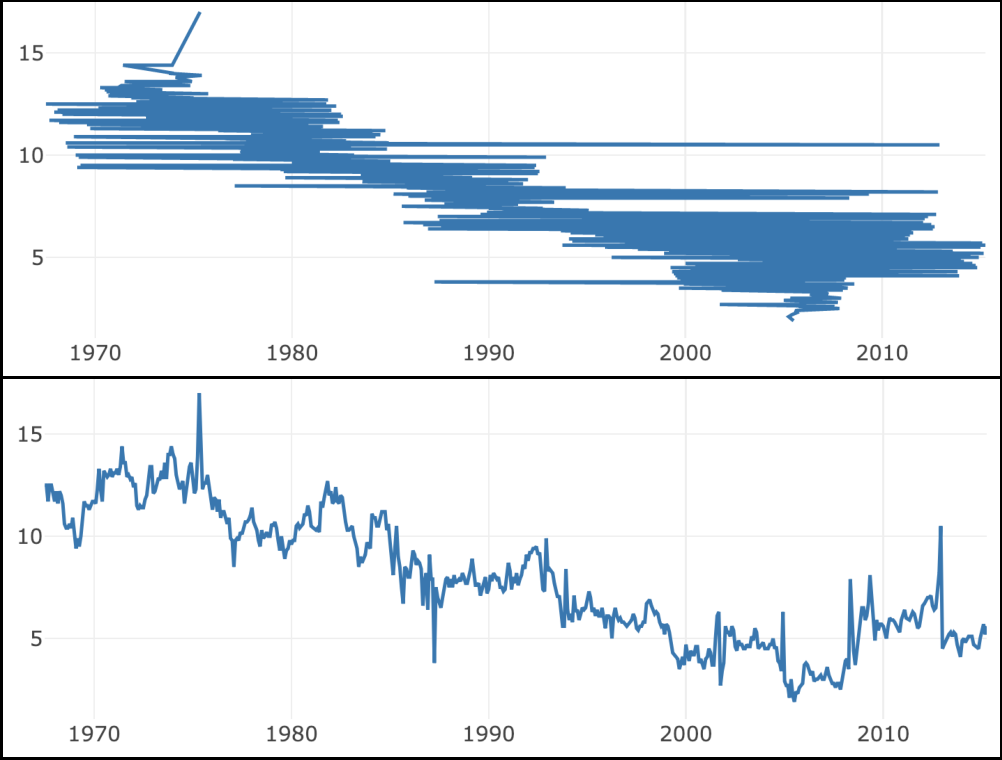
\includegraphics[width=\textwidth]{images/scatter-intro} 

}

\caption{The difference between \texttt{add\_paths()} and \texttt{add\_lines()}: the top panel connects observations according to the ordering of \texttt{psavert} (personal savings rate), whereas the bottom panel connects observations according to the ordering of \texttt{x} (the date).}\label{fig:scatter-intro}
\end{figure}

Section \ref{intro-plotly} introduced `aesthetic mapping' arguments (unique to the R package) which make it easier to map data to visual properties (e.g., \texttt{color}, \texttt{linetype}, etc). In addition to these arguments, \textbf{dplyr} groupings can be used to ensure there is at least one geometry per group. The top panel of Figure \ref{fig:scatter-intro} demonstrates how \texttt{group\_by()} could be used to effectively wrap the time series from Figure \ref{fig:scatter-intro} by year, which can be useful for visualizing annual seasonality. Another approach to generating at least one geometry per `group' is to provide categorical variable to a relevant aesthetic (e.g., \texttt{color}), as shown in the bottom panel of Figure \ref{fig:scatter-intro}.

\index{plot\_ly()@\texttt{plot\_ly()}!group\_by()@\texttt{group\_by()} vs \texttt{split}}

\begin{Shaded}
\begin{Highlighting}[]
\KeywordTok{library}\NormalTok{(lubridate)}
\NormalTok{econ <-}\StringTok{ }\NormalTok{economics }\OperatorTok
\StringTok{  }\KeywordTok{mutate}\NormalTok{(}\DataTypeTok{yr =} \KeywordTok{year}\NormalTok{(date), }\DataTypeTok{mnth =} \KeywordTok{month}\NormalTok{(date))}

\CommentTok{# One trace (more performant, but less interactive)}
\NormalTok{econ }\OperatorTok
\StringTok{  }\KeywordTok{group_by}\NormalTok{(yr) }\OperatorTok
\StringTok{  }\KeywordTok{plot_ly}\NormalTok{(}\DataTypeTok{x =} \OperatorTok{~}\NormalTok{mnth, }\DataTypeTok{y =} \OperatorTok{~}\NormalTok{uempmed) }\OperatorTok
\StringTok{  }\KeywordTok{add_lines}\NormalTok{(}\DataTypeTok{text =} \OperatorTok{~}\NormalTok{yr)}

\CommentTok{# Multiple traces (less performant, but more interactive)}
\KeywordTok{plot_ly}\NormalTok{(econ, }\DataTypeTok{x =} \OperatorTok{~}\NormalTok{mnth, }\DataTypeTok{y =} \OperatorTok{~}\NormalTok{uempmed) }\OperatorTok
\StringTok{  }\KeywordTok{add_lines}\NormalTok{(}\DataTypeTok{color =} \OperatorTok{~}\KeywordTok{ordered}\NormalTok{(yr))}
  
\CommentTok{# The split argument guarantees one trace per group level (regardless }
\CommentTok{# of the variable type). This is useful if you want a consistent visual}
\CommentTok{# property over multiple traces }
\CommentTok{# plot_ly(econ, x = ~mnth, y = ~uempmed) %>%}
\CommentTok{#   add_lines(split = ~yr, color = I("black"))}
\end{Highlighting}
\end{Shaded}

\begin{figure}

{\centering 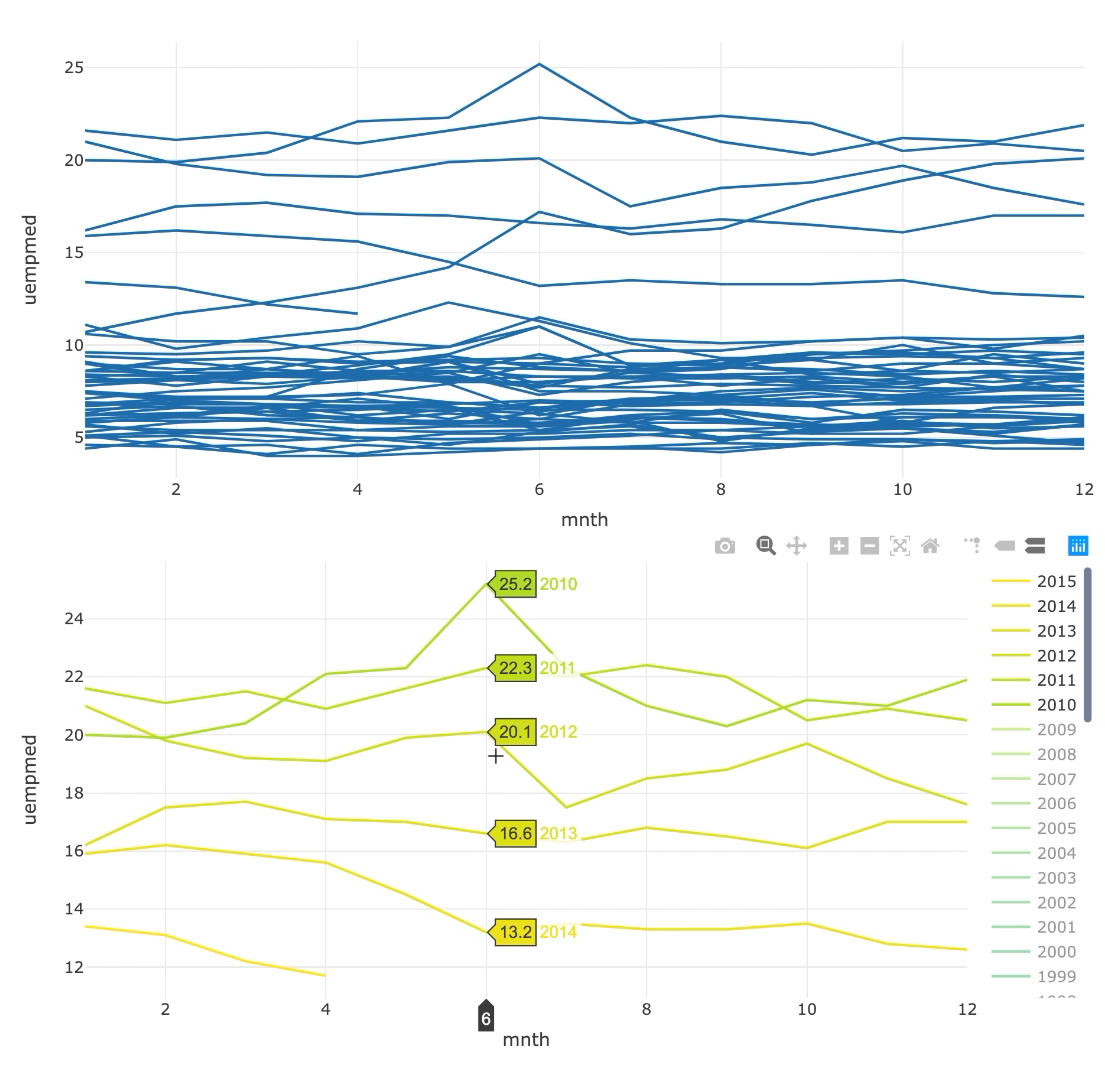
\includegraphics[width=\textwidth]{vimeo-images/316679591/final} 

}

\caption{Drawing multiple lines using \textbf{dplyr} groups (top panel) versus a categorical \texttt{color} mapping (bottom panel). Comparatively speaking, the bottom panel has more interactive capabilities (e.g., legend-based filtering and multiple tooltips), but it does not scale as well with many lines. For a video demonstration of the interactive, see \url{https://bit.ly/scatter-lines}. For the interactive, see \url{https://plotly-r.com/interactives/scatter-lines.html}}\label{fig:scatter-lines}
\end{figure}

Not only do these plots differ in visual appearance, they also differ in interactive capabilities, computational performance, and underlying implementation. That's because, the grouping approach (top panel of Figure \ref{fig:scatter-lines}) uses just one plotly.js trace (more performant, less interactive), whereas the \texttt{color} approach (bottom panel of Figure \ref{fig:scatter-lines}) generates one trace per line/year. In this case, the benefit of having multiple traces is that we can perform interactive filtering via the legend and compare multiple y-values at a given x. The cost of having those capabilities is that plots starts to be become sluggish after a few hundred traces, whereas thousands of lines can be rendered fairly easily in one trace. See Chapter \ref{performance} for more details on scaling and performance.

\index{add\_trace()@\texttt{add\_trace()}}
\index{plot\_ly()@\texttt{plot\_ly()}!Special attributes}
\index{layout()@\texttt{layout()}!2D Axes!range@\texttt{range}}

These features make it easier to get started using plotly.js, but it still pays off to learn how to use plotly.js directly. You won't find plotly.js attributes listed as explicit arguments in any \textbf{plotly} function (except for the special \texttt{type} attribute), but they are passed along verbatim to the plotly.js figure definition through the \texttt{...} operator. The scatter-based layers in this chapter fix the \texttt{type} plotly.js attribute to \texttt{"scatter"} as well as the \href{https://plot.ly/r/reference/\#scatter-mode}{\texttt{mode}} (e.g., \texttt{add\_markers()} uses \texttt{mode=\textquotesingle{}markers\textquotesingle{}} etc), but you could also use the lower-level \texttt{add\_trace()} to work more directly with plotly.js. For example, Figure \ref{fig:tooltip-praise} shows how to render markers, lines, and text in the same scatter trace. It also demonstrates how to leverage \emph{nested} plotly.js attributes, like \href{https://plot.ly/r/reference/\#scatter-textfont}{\texttt{textfont}} and \href{https://plot.ly/r/reference/\#layout-xaxis}{\texttt{xaxis}} -- these attributes contain other attributes, so you need to supply a suitable named list to these arguments.

\begin{Shaded}
\begin{Highlighting}[]
\KeywordTok{set.seed}\NormalTok{(}\DecValTok{99}\NormalTok{)}
\KeywordTok{plot_ly}\NormalTok{() }\OperatorTok
\StringTok{ }\KeywordTok{add_trace}\NormalTok{(}
   \DataTypeTok{type =} \StringTok{"scatter"}\NormalTok{,}
   \DataTypeTok{mode =} \StringTok{"markers+lines+text"}\NormalTok{,}
   \DataTypeTok{x =} \DecValTok{4}\OperatorTok{:}\DecValTok{6}\NormalTok{, }
   \DataTypeTok{y =} \DecValTok{4}\OperatorTok{:}\DecValTok{6}\NormalTok{,}
   \DataTypeTok{text =} \KeywordTok{replicate}\NormalTok{(}\DecValTok{3}\NormalTok{, praise}\OperatorTok{::}\KeywordTok{praise}\NormalTok{(}\StringTok{"You are $\{adjective\}! 🙌"}\NormalTok{)),}
   \DataTypeTok{textposition =} \StringTok{"right"}\NormalTok{,}
   \DataTypeTok{hoverinfo =} \StringTok{"text"}\NormalTok{,}
   \DataTypeTok{textfont =} \KeywordTok{list}\NormalTok{(}\DataTypeTok{family =} \StringTok{"Roboto Condensed"}\NormalTok{, }\DataTypeTok{size =} \DecValTok{16}\NormalTok{)}
\NormalTok{ ) }\OperatorTok
\StringTok{ }\KeywordTok{layout}\NormalTok{(}\DataTypeTok{xaxis =} \KeywordTok{list}\NormalTok{(}\DataTypeTok{range =} \KeywordTok{c}\NormalTok{(}\DecValTok{3}\NormalTok{, }\DecValTok{8}\NormalTok{)))}
\end{Highlighting}
\end{Shaded}

\begin{figure}

{\centering 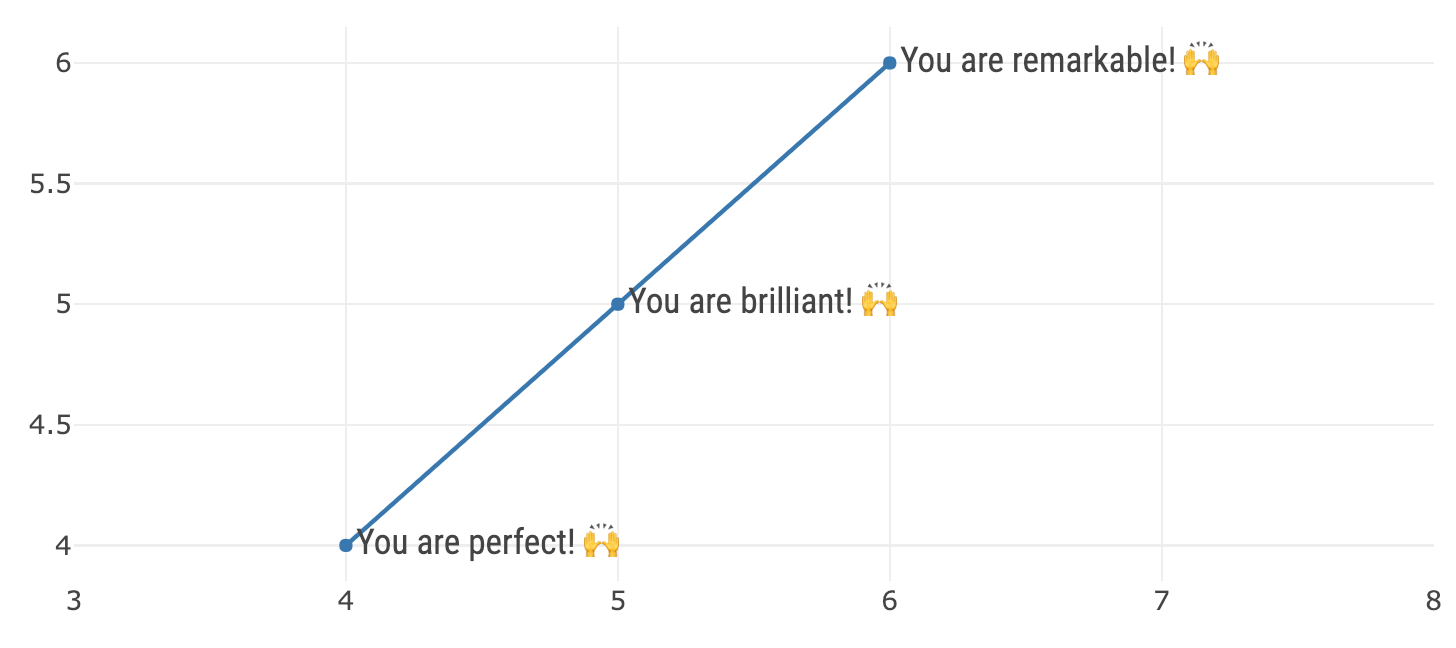
\includegraphics[width=\textwidth]{images/tooltip-praise} 

}

\caption{Using the generic \texttt{add\_trace()} function to render markers, lines, and text in a single scatter trace. This \texttt{add\_trace()} function, as well as any \texttt{add\_*()} function allows you to directly specify plotly.js attributes.}\label{fig:tooltip-praise}
\end{figure}

\index{Plotly figure!Reference}
\index{schema()@\texttt{schema()}|seealso {Reference}}

If you are new to plotly.js, I recommend taking a bit of time to look through the plotly.js attributes that are available to the scatter trace type and think how you might be able to use them. Most of these attributes work for other trace types as well, so learning an attribute once for a specific plot can pay off in other contexts as well. The online plotly.js figure reference, \url{https://plot.ly/r/reference/\#scatter}, is a decent place to search and learn about the attributes, but I recommend using the \texttt{schema()} function instead for a few reasons:

\begin{itemize}
\tightlist
\item
  \texttt{schema()} provides a bit more information than the online docs (e.g., value types, default values, acceptable ranges, etc).
\item
  The interface makes it a bit easier to traverse and discover new attributes.
\item
  You can be absolutely sure it matches the version used in the R package (the online docs might use a different -- probably older -- version).
\end{itemize}

\begin{Shaded}
\begin{Highlighting}[]
\KeywordTok{schema}\NormalTok{()}
\end{Highlighting}
\end{Shaded}

\begin{figure}

{\centering 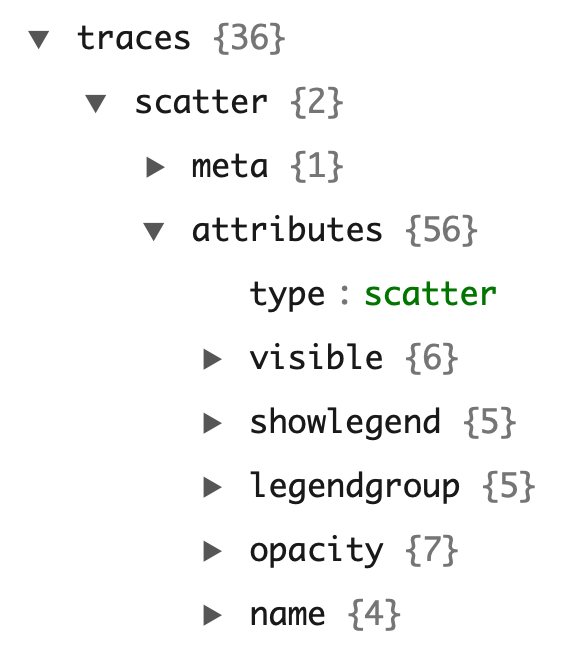
\includegraphics[width=0.4\linewidth]{images/schema} 

}

\caption{Using \texttt{schema()} function to traverse through the attributes available to a given trace type (e.g., scatter)}\label{fig:schema}
\end{figure}

The sections that follow in this chapter demonstrate various type of data views using scatter-based layers. In attempt to avoid duplication of documentation, a particular emphasis is put on features only currently availbale from the R package (e.g., the aesthetic mapping arguments).

\hypertarget{markers}{%
\section{Markers}\label{markers}}

\index{add\_trace()@\texttt{add\_trace()}!add\_markers()@\texttt{add\_markers()}}

This section details scatter traces with a \texttt{mode} of \texttt{"markers"} (i.e., \texttt{add\_markers()}). For simplicity, many of the examples here use \texttt{add\_markers()} with a numeric x and y axis, which results in scatterplot -- a common way to visualize the association between two quantitative variables. The content that follows is still relevant markers displayed non-numeric x and y (aka dot pots) as shown in Section \ref{dot-plots}.

\hypertarget{marker-alpha}{%
\subsection{Alpha blending}\label{marker-alpha}}

\index{plot\_ly()@\texttt{plot\_ly()}!Special attributes!alpha@\texttt{alpha}}

As \citet{unwin-graphical-analysis} notes, scatterplots can be useful for exposing other important features including: casual relationships, outliers, clusters, gaps, barriers, and conditional relationships. A common problem with scatterplots, however is overplotting, meaning that there are multiple observations occupying the same (or similar) x/y locations. Figure \ref{fig:scatterplots} demonstrates one way to combat overplotting via alpha blending. When dealing with tens of thousands of points (or more), consider using \texttt{toWebGL()} to render plots using Canvas rather than SVG (more in Chapter \ref{performance}, or leveraging 2D density estimation (Section \ref{rectangular-binning-in-r}).

\begin{Shaded}
\begin{Highlighting}[]
\KeywordTok{subplot}\NormalTok{(}
  \KeywordTok{plot_ly}\NormalTok{(mpg, }\DataTypeTok{x =} \OperatorTok{~}\NormalTok{cty, }\DataTypeTok{y =} \OperatorTok{~}\NormalTok{hwy, }\DataTypeTok{name =} \StringTok{"default"}\NormalTok{),}
  \KeywordTok{plot_ly}\NormalTok{(mpg, }\DataTypeTok{x =} \OperatorTok{~}\NormalTok{cty, }\DataTypeTok{y =} \OperatorTok{~}\NormalTok{hwy) }\OperatorTok\StringTok{ }
\StringTok{    }\KeywordTok{add_markers}\NormalTok{(}\DataTypeTok{alpha =} \FloatTok{0.2}\NormalTok{, }\DataTypeTok{name =} \StringTok{"alpha"}\NormalTok{)}
\NormalTok{)}
\end{Highlighting}
\end{Shaded}

\begin{figure}

{\centering 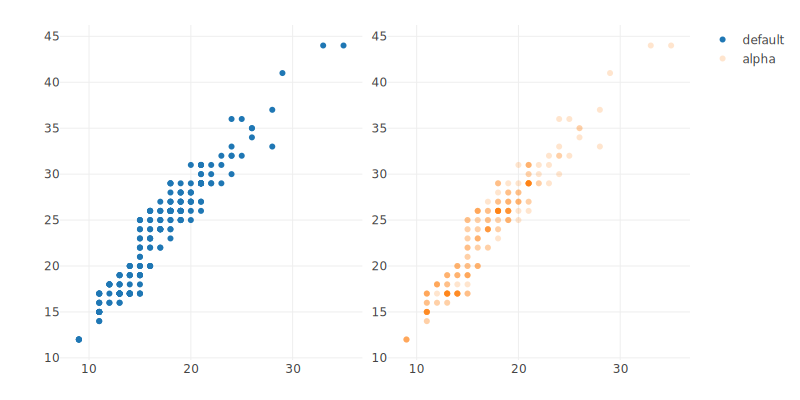
\includegraphics[width=\textwidth]{images/scatterplots} 

}

\caption{Combating overplotting in a scatterplot with alpha blending.}\label{fig:scatterplots}
\end{figure}

\hypertarget{marker-color}{%
\subsection{Colors}\label{marker-color}}

\index{plot\_ly()@\texttt{plot\_ly()}!Special attributes!color@\texttt{color} / \texttt{colors}}
\index{colorbar()@\texttt{colorbar()}}

As discussed in Section \ref{intro-plotly-js}, mapping a discrete variable to \texttt{color} produces one trace per category, which is desirable for it's legend and hover properties. On the other hand, mapping a \emph{numeric} variable to \texttt{color} produces one trace, as well as a \href{https://plot.ly/r/reference/\#scatter-marker-colorbar}{colorbar} guide for visually decoding colors back to data values. The \texttt{colorbar()} function can be used to customize the appearance of this automatically generated guide. The default colorscale is viridis, a perceptually-uniform colorscale (even when converted to black-and-white), and perceivable even to those with common forms of color blindness \citep{viridis}. Viridis is also the default colorscale for ordered factors.

\begin{Shaded}
\begin{Highlighting}[]
\NormalTok{p <-}\StringTok{ }\KeywordTok{plot_ly}\NormalTok{(mpg, }\DataTypeTok{x =} \OperatorTok{~}\NormalTok{cty, }\DataTypeTok{y =} \OperatorTok{~}\NormalTok{hwy, }\DataTypeTok{alpha =} \FloatTok{0.5}\NormalTok{)}
\KeywordTok{subplot}\NormalTok{(}
  \KeywordTok{add_markers}\NormalTok{(p, }\DataTypeTok{color =} \OperatorTok{~}\NormalTok{cyl, }\DataTypeTok{showlegend =} \OtherTok{FALSE}\NormalTok{) }\OperatorTok\StringTok{ }
\StringTok{    }\KeywordTok{colorbar}\NormalTok{(}\DataTypeTok{title =} \StringTok{"Viridis"}\NormalTok{),}
  \KeywordTok{add_markers}\NormalTok{(p, }\DataTypeTok{color =} \OperatorTok{~}\KeywordTok{factor}\NormalTok{(cyl))}
\NormalTok{)}
\end{Highlighting}
\end{Shaded}

\begin{figure}

{\centering 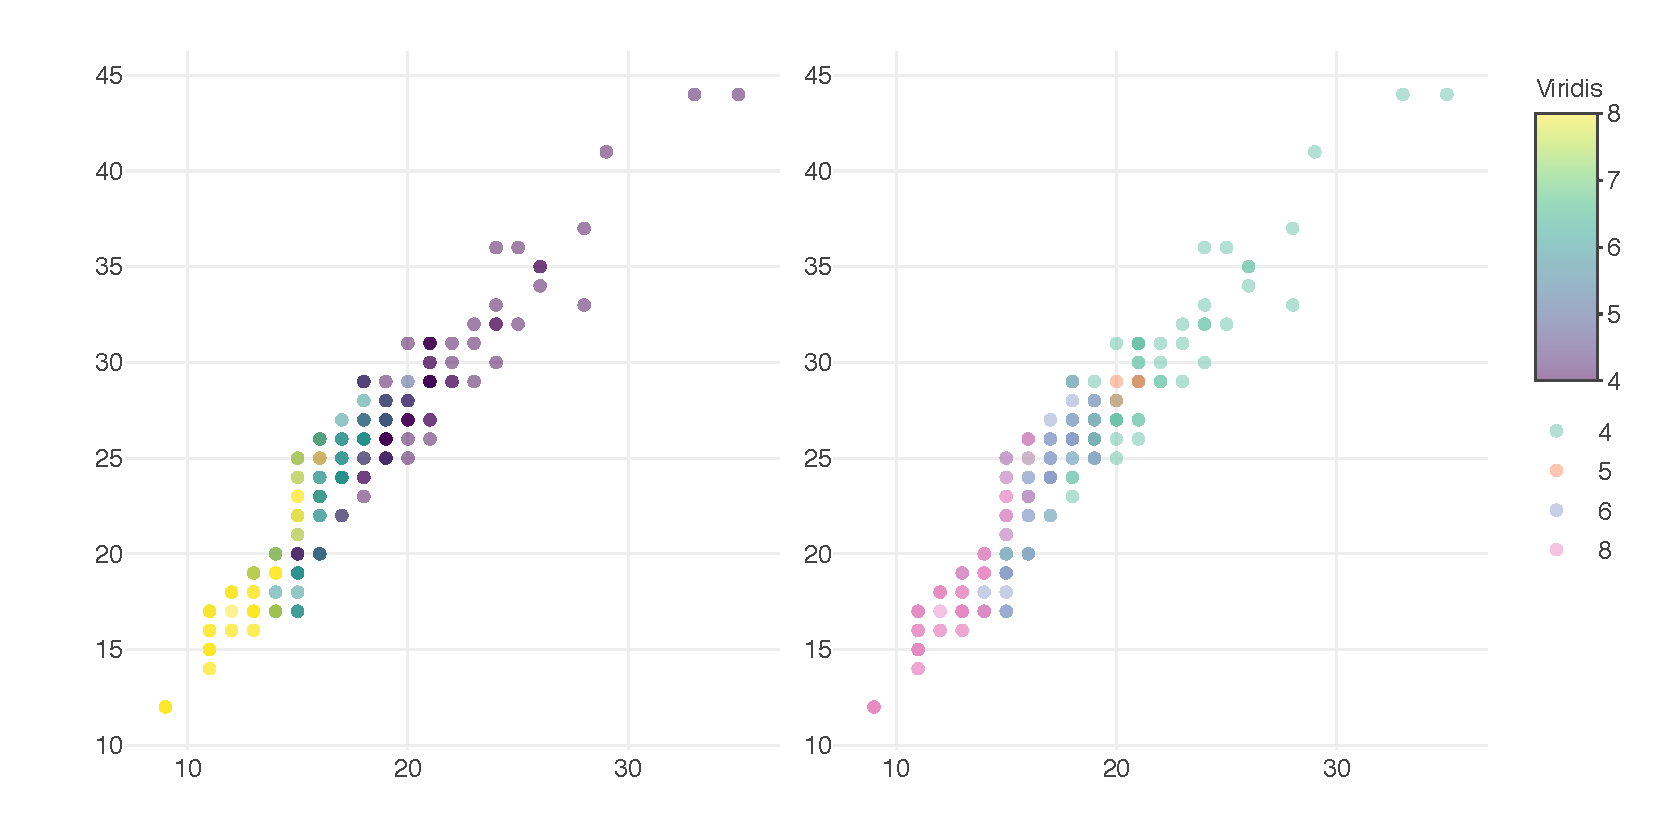
\includegraphics[width=\textwidth]{images/color-types} 

}

\caption{Variations on a numeric color mapping.}\label{fig:color-types}
\end{figure}

There are numerous ways to alter the default color scale via the \texttt{colors} argument. This argument excepts one of the following: (1) a color brewer palette name (see the row names of \texttt{RColorBrewer::brewer.pal.info} for valid names), (2) a vector of colors to interpolate, or (3) a color interpolation function like \texttt{colorRamp()} or \texttt{scales::colour\_ramp()}. Although this grants a lot of flexibility, one should be conscious of using a sequential colorscale for numeric variables (\& ordered factors) as shown in Figure \ref{fig:color-numeric}, and a qualitative colorscale for discrete variables as shown in Figure \ref{fig:color-discrete}.

\begin{Shaded}
\begin{Highlighting}[]
\NormalTok{col1 <-}\StringTok{ }\KeywordTok{c}\NormalTok{(}\StringTok{"#132B43"}\NormalTok{, }\StringTok{"#56B1F7"}\NormalTok{)}
\NormalTok{col2 <-}\StringTok{ }\NormalTok{viridisLite}\OperatorTok{::}\KeywordTok{inferno}\NormalTok{(}\DecValTok{10}\NormalTok{)}
\NormalTok{col3 <-}\StringTok{ }\KeywordTok{colorRamp}\NormalTok{(}\KeywordTok{c}\NormalTok{(}\StringTok{"red"}\NormalTok{, }\StringTok{"white"}\NormalTok{, }\StringTok{"blue"}\NormalTok{))}
\KeywordTok{subplot}\NormalTok{(}
  \KeywordTok{add_markers}\NormalTok{(p, }\DataTypeTok{color =} \OperatorTok{~}\NormalTok{cyl, }\DataTypeTok{colors =}\NormalTok{ col1) }\OperatorTok
\StringTok{    }\KeywordTok{colorbar}\NormalTok{(}\DataTypeTok{title =} \StringTok{"ggplot2 default"}\NormalTok{),}
  \KeywordTok{add_markers}\NormalTok{(p, }\DataTypeTok{color =} \OperatorTok{~}\NormalTok{cyl, }\DataTypeTok{colors =}\NormalTok{ col2) }\OperatorTok\StringTok{ }
\StringTok{    }\KeywordTok{colorbar}\NormalTok{(}\DataTypeTok{title =} \StringTok{"Inferno"}\NormalTok{),}
  \KeywordTok{add_markers}\NormalTok{(p, }\DataTypeTok{color =} \OperatorTok{~}\NormalTok{cyl, }\DataTypeTok{colors =}\NormalTok{ col3) }\OperatorTok\StringTok{ }
\StringTok{    }\KeywordTok{colorbar}\NormalTok{(}\DataTypeTok{title =} \StringTok{"colorRamp"}\NormalTok{)}
\NormalTok{) }\OperatorTok\StringTok{ }\KeywordTok{hide_legend}\NormalTok{()}
\end{Highlighting}
\end{Shaded}

\begin{figure}

{\centering 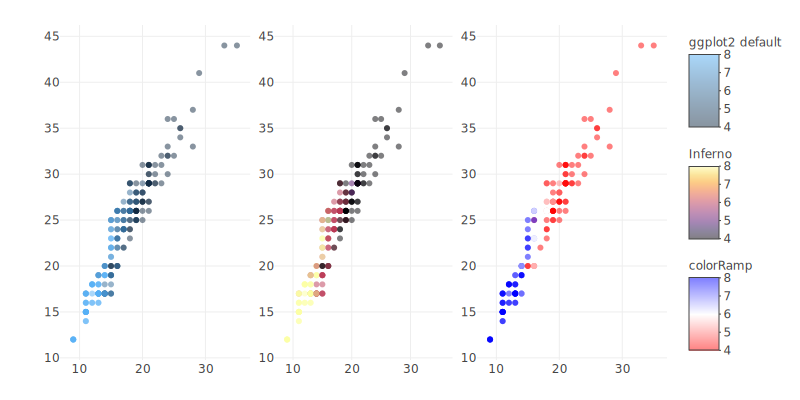
\includegraphics[width=\textwidth]{images/color-numeric} 

}

\caption{Three variations on a numeric color mapping.}\label{fig:color-numeric}
\end{figure}

\begin{Shaded}
\begin{Highlighting}[]
\NormalTok{col1 <-}\StringTok{ "Accent"}
\NormalTok{col2 <-}\StringTok{ }\KeywordTok{colorRamp}\NormalTok{(}\KeywordTok{c}\NormalTok{(}\StringTok{"red"}\NormalTok{, }\StringTok{"blue"}\NormalTok{))}
\NormalTok{col3 <-}\StringTok{ }\KeywordTok{c}\NormalTok{(}\StringTok{`}\DataTypeTok{4}\StringTok{`}\NormalTok{ =}\StringTok{ "red"}\NormalTok{, }\StringTok{`}\DataTypeTok{5}\StringTok{`}\NormalTok{ =}\StringTok{ "black"}\NormalTok{, }\StringTok{`}\DataTypeTok{6}\StringTok{`}\NormalTok{ =}\StringTok{ "blue"}\NormalTok{, }\StringTok{`}\DataTypeTok{8}\StringTok{`}\NormalTok{ =}\StringTok{ "green"}\NormalTok{)}
\KeywordTok{subplot}\NormalTok{(}
  \KeywordTok{add_markers}\NormalTok{(p, }\DataTypeTok{color =} \OperatorTok{~}\KeywordTok{factor}\NormalTok{(cyl), }\DataTypeTok{colors =}\NormalTok{ col1),}
  \KeywordTok{add_markers}\NormalTok{(p, }\DataTypeTok{color =} \OperatorTok{~}\KeywordTok{factor}\NormalTok{(cyl), }\DataTypeTok{colors =}\NormalTok{ col2),}
  \KeywordTok{add_markers}\NormalTok{(p, }\DataTypeTok{color =} \OperatorTok{~}\KeywordTok{factor}\NormalTok{(cyl), }\DataTypeTok{colors =}\NormalTok{ col3)}
\NormalTok{) }\OperatorTok\StringTok{ }\KeywordTok{hide_legend}\NormalTok{()}
\end{Highlighting}
\end{Shaded}

\begin{figure}

{\centering 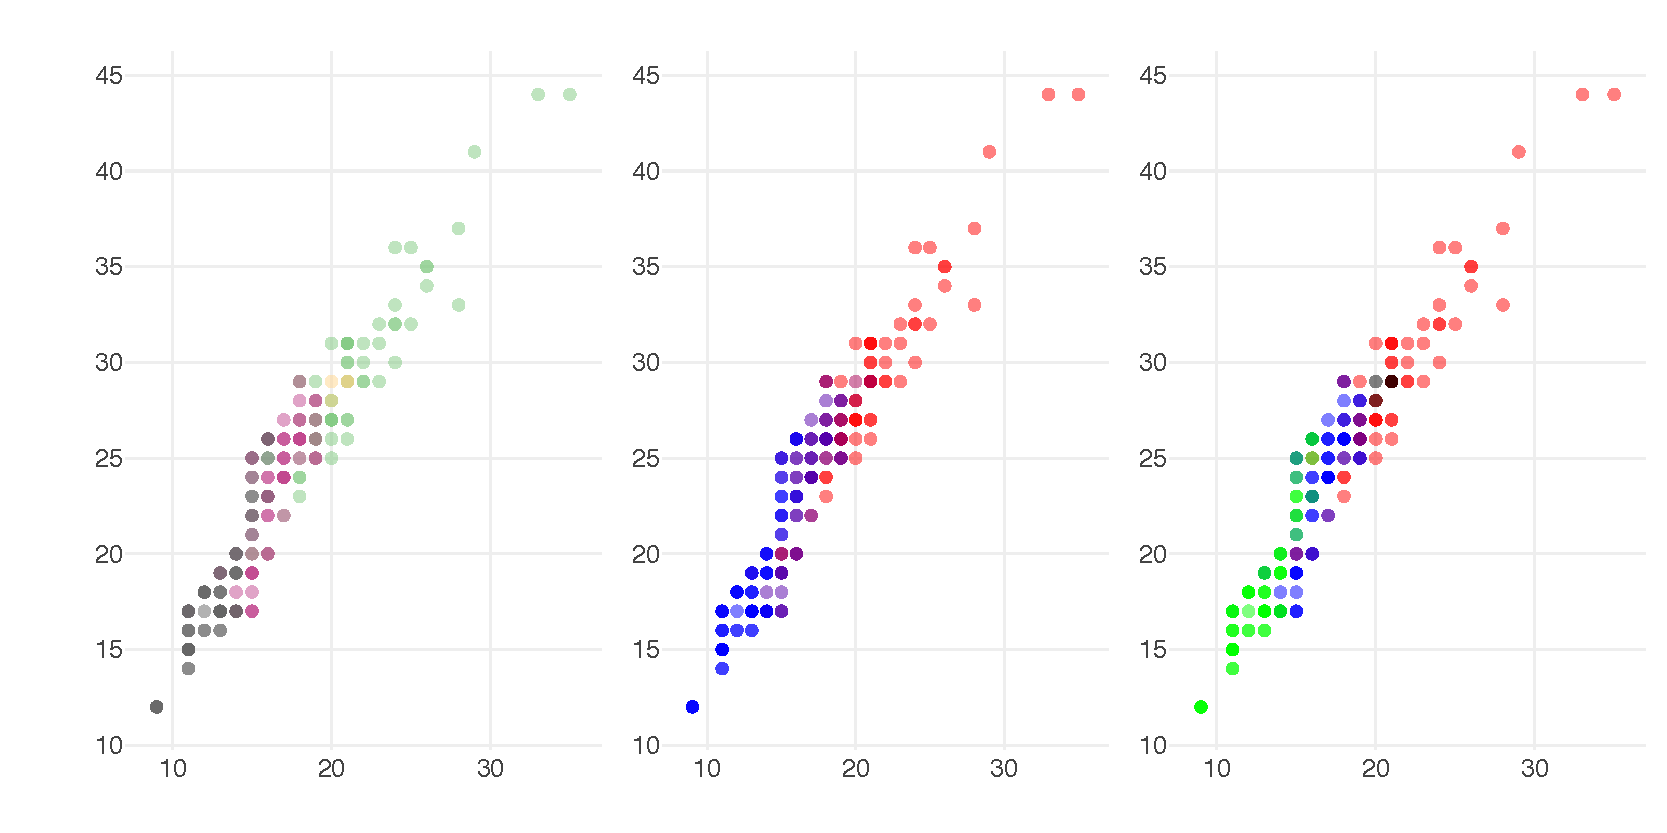
\includegraphics[width=\textwidth]{images/color-discrete} 

}

\caption{Three variations on a discrete color mapping.}\label{fig:color-discrete}
\end{figure}

As introduced in Figure \ref{fig:intro-range}, color codes can be specified manually (i.e., avoid mapping data values to a visual range) by using the \texttt{I()} function. Figure \ref{fig:color-manual} provides a simple example using \texttt{add\_markers()}. Any color understood by the \texttt{col2rgb()} function from the \textbf{grDevices} package can be used in this way. Chapter \ref{working-with-colors} provides even more details about working with different color specifications when specifying colors manually.

\begin{Shaded}
\begin{Highlighting}[]
\KeywordTok{add_markers}\NormalTok{(p, }\DataTypeTok{color =} \KeywordTok{I}\NormalTok{(}\StringTok{"black"}\NormalTok{))}
\end{Highlighting}
\end{Shaded}

\begin{figure}

{\centering 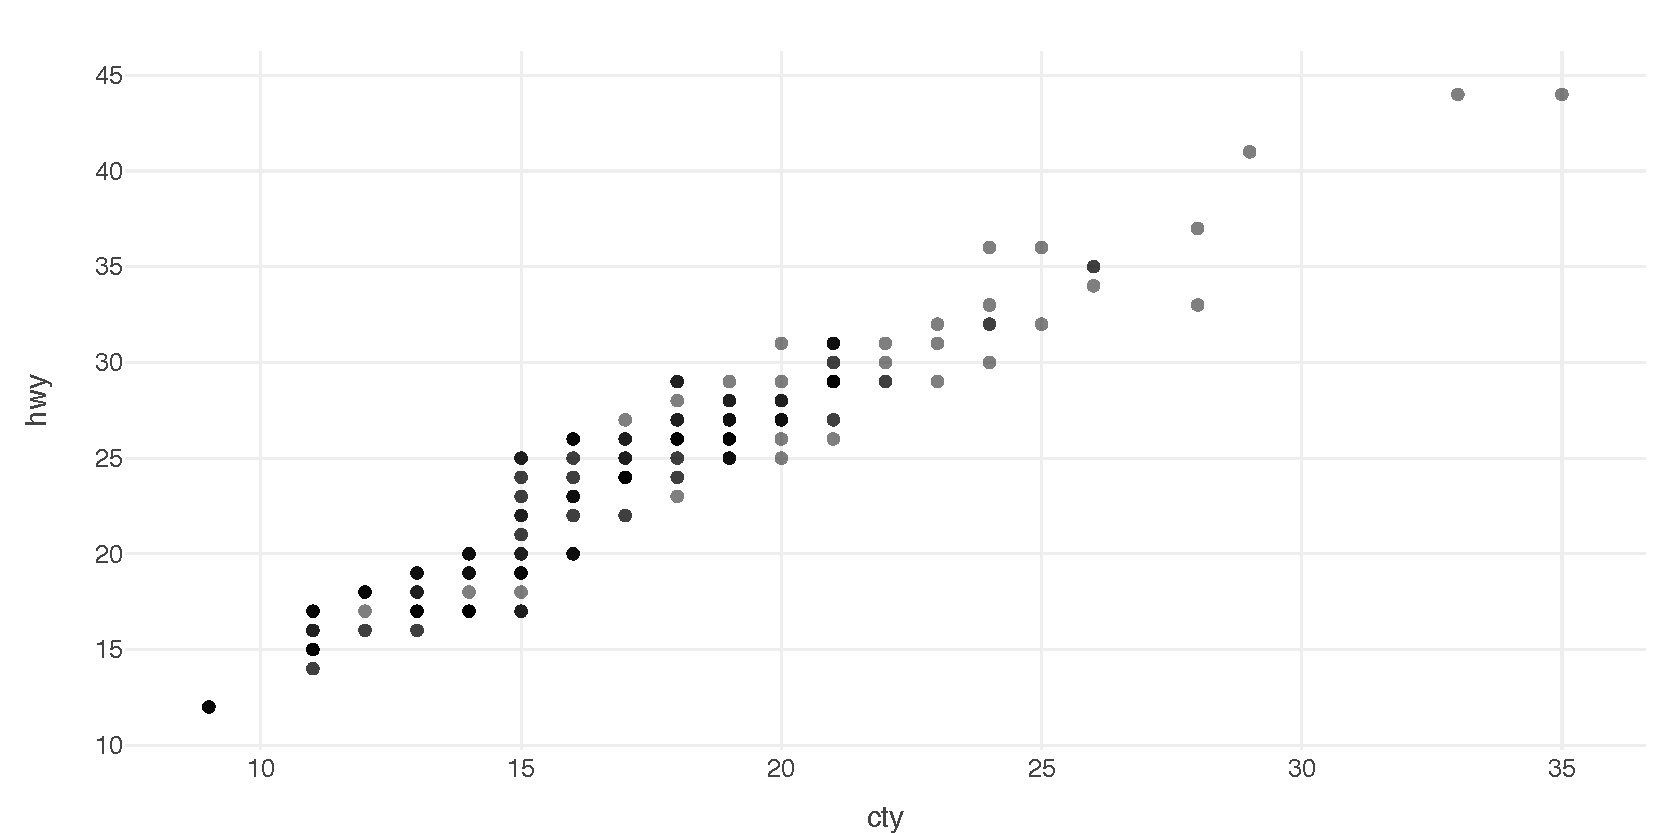
\includegraphics[width=\textwidth]{images/color-manual} 

}

\caption{Setting a fixed color directly using \texttt{I()}.}\label{fig:color-manual}
\end{figure}

The \texttt{color} argument is meant to control the `fill-color' of a geometric object, whereas \texttt{stroke} (Section \ref{marker-stroke}) is meant to control the `outline-color' of a geometric object. In the case of \texttt{add\_markers()}, that means \texttt{color} maps to the plotly.js attribute \href{https://plot.ly/r/reference/\#scatter-marker-color}{\texttt{marker.color}} and \texttt{stroke} maps to \href{https://plot.ly/r/reference/\#scatter-marker-line-color}{\texttt{marker.line.color}}. Not all, but many, marker symbols have a notion of stroke.

\hypertarget{marker-symbol}{%
\subsection{Symbols}\label{marker-symbol}}

\index{plot\_ly()@\texttt{plot\_ly()}!Special attributes!symbol@\texttt{symbol} / \texttt{symbols}}

The \texttt{symbol} argument can be used to map data values to the \texttt{marker.symbol} plotly.js attribute. It uses the same semantics that we've already seen for \texttt{color}:

\begin{itemize}
\tightlist
\item
  A numeric mapping generates trace.
\item
  A discrete mapping generates multiple traces (one trace per category).
\item
  The plural, \texttt{symbols}, can be used to specify the visual range for the mapping.
\item
  Mappings are avoided entirely through \texttt{I()}.
\end{itemize}

For example, the left panel of Figure \ref{fig:symbol-factor} uses a numeric mapping and the right panel uses a discrete mapping. As a result, the left panel is linked to the first legend entry, whereas the right panel is linked to the bottom three legend entries. When plotting multiple traces and no color is specifeid, the plotly.js \href{https://plot.ly/r/reference/\#layout-colorway}{colorway} is applied (i.e., each trace will be rendered a different color). To set a fixed color, you can set the color of every trace generated from this layer with \texttt{color\ =\ I("black")}, or similar.

\begin{Shaded}
\begin{Highlighting}[]
\NormalTok{p <-}\StringTok{ }\KeywordTok{plot_ly}\NormalTok{(mpg, }\DataTypeTok{x =} \OperatorTok{~}\NormalTok{cty, }\DataTypeTok{y =} \OperatorTok{~}\NormalTok{hwy, }\DataTypeTok{alpha =} \FloatTok{0.3}\NormalTok{) }
\KeywordTok{subplot}\NormalTok{(}
  \KeywordTok{add_markers}\NormalTok{(p, }\DataTypeTok{symbol =} \OperatorTok{~}\NormalTok{cyl, }\DataTypeTok{name =} \StringTok{"A single trace"}\NormalTok{),}
  \KeywordTok{add_markers}\NormalTok{(p, }\DataTypeTok{symbol =} \OperatorTok{~}\KeywordTok{factor}\NormalTok{(cyl), }\DataTypeTok{color =} \KeywordTok{I}\NormalTok{(}\StringTok{"black"}\NormalTok{))}
\NormalTok{)}
\end{Highlighting}
\end{Shaded}

\begin{figure}

{\centering 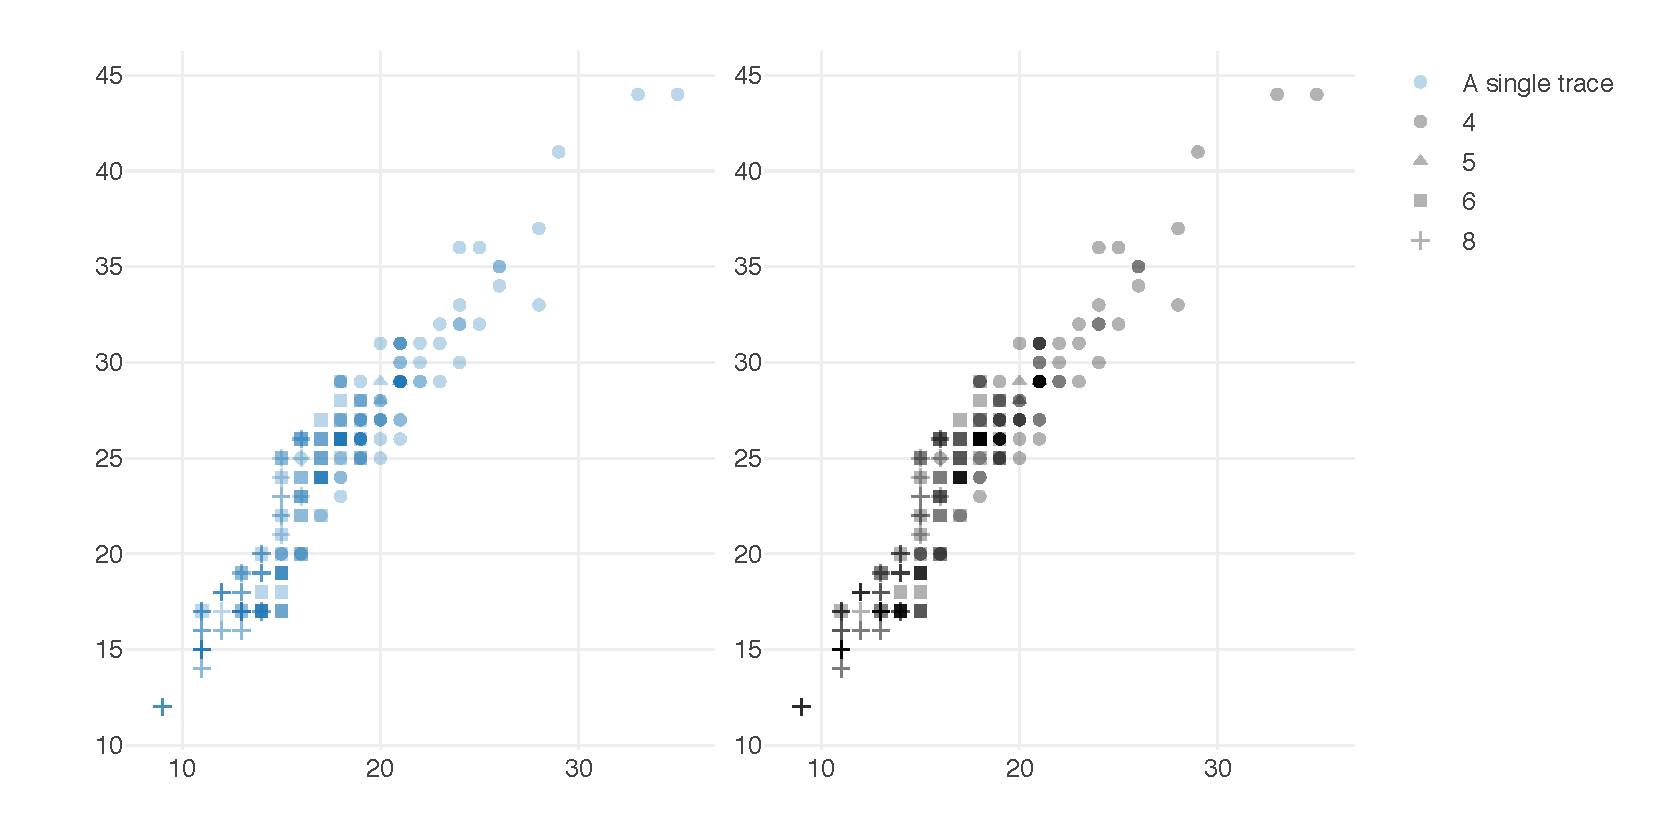
\includegraphics[width=\textwidth]{images/symbol-factor} 

}

\caption{Mapping symbol to a numeric variable (left panel) and a factor (right panel).}\label{fig:symbol-factor}
\end{figure}

There are two ways to specify the visual range of \texttt{symbols}: (1) numeric codes (interpreted as a \texttt{pch} codes) or (2) a character string specifying a valid \texttt{marker.symbol} value. Figure \ref{fig:symbol-factor-range} uses pch codes (left panel) as well as their corresponding \texttt{marker.symbol} name (right panel) to specify the visual range.

\begin{Shaded}
\begin{Highlighting}[]
\KeywordTok{subplot}\NormalTok{(}
  \KeywordTok{add_markers}\NormalTok{(p, }\DataTypeTok{symbol =} \OperatorTok{~}\NormalTok{cyl, }\DataTypeTok{symbols =} \KeywordTok{c}\NormalTok{(}\DecValTok{17}\NormalTok{, }\DecValTok{18}\NormalTok{, }\DecValTok{19}\NormalTok{)),}
  \KeywordTok{add_markers}\NormalTok{(}
\NormalTok{    p, }\DataTypeTok{color =} \KeywordTok{I}\NormalTok{(}\StringTok{"black"}\NormalTok{),}
    \DataTypeTok{symbol =} \OperatorTok{~}\KeywordTok{factor}\NormalTok{(cyl), }
    \DataTypeTok{symbols =} \KeywordTok{c}\NormalTok{(}\StringTok{"triangle-up"}\NormalTok{, }\StringTok{"diamond"}\NormalTok{, }\StringTok{"circle"}\NormalTok{)}
\NormalTok{  )}
\NormalTok{)}
\end{Highlighting}
\end{Shaded}

\begin{figure}

{\centering 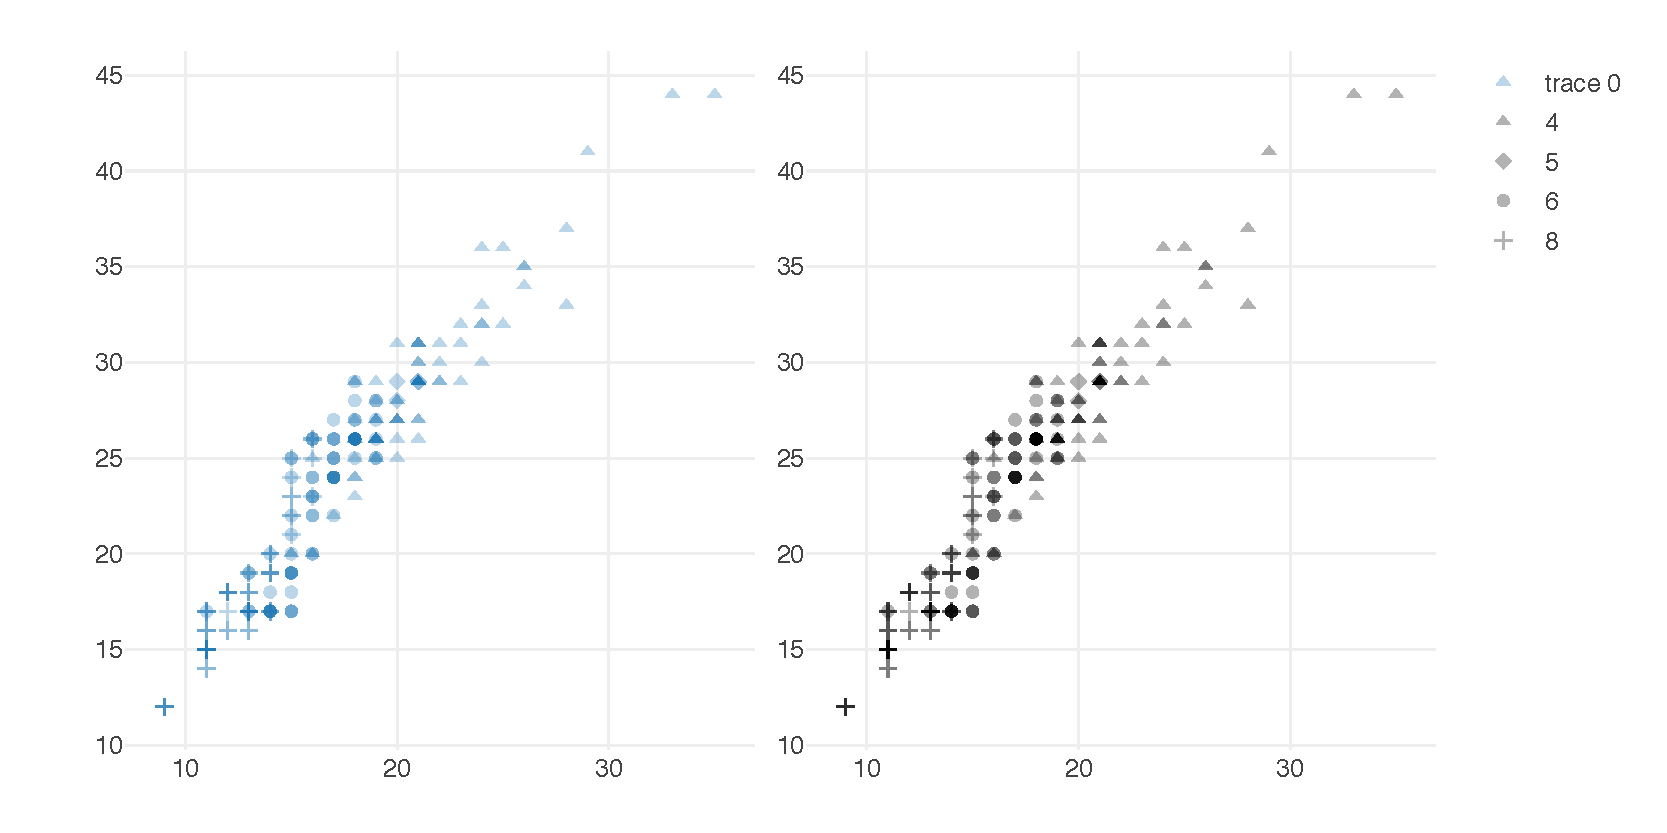
\includegraphics[width=\textwidth]{images/symbol-factor-range} 

}

\caption{Specifying the visual range of \texttt{symbols}.}\label{fig:symbol-factor-range}
\end{figure}

These \texttt{symbols} (i.e., the visual range) can also be supplied directly to \texttt{symbol} through \texttt{I()}. For example, Figure \ref{fig:symbol-factor-manual} fixes the marker symbol to a diamond shape.

\begin{Shaded}
\begin{Highlighting}[]
\KeywordTok{plot_ly}\NormalTok{(mpg, }\DataTypeTok{x =} \OperatorTok{~}\NormalTok{cty, }\DataTypeTok{y =} \OperatorTok{~}\NormalTok{hwy) }\OperatorTok
\StringTok{  }\KeywordTok{add_markers}\NormalTok{(}\DataTypeTok{symbol =} \KeywordTok{I}\NormalTok{(}\DecValTok{18}\NormalTok{), }\DataTypeTok{alpha =} \FloatTok{0.5}\NormalTok{)}
\end{Highlighting}
\end{Shaded}

\begin{figure}

{\centering 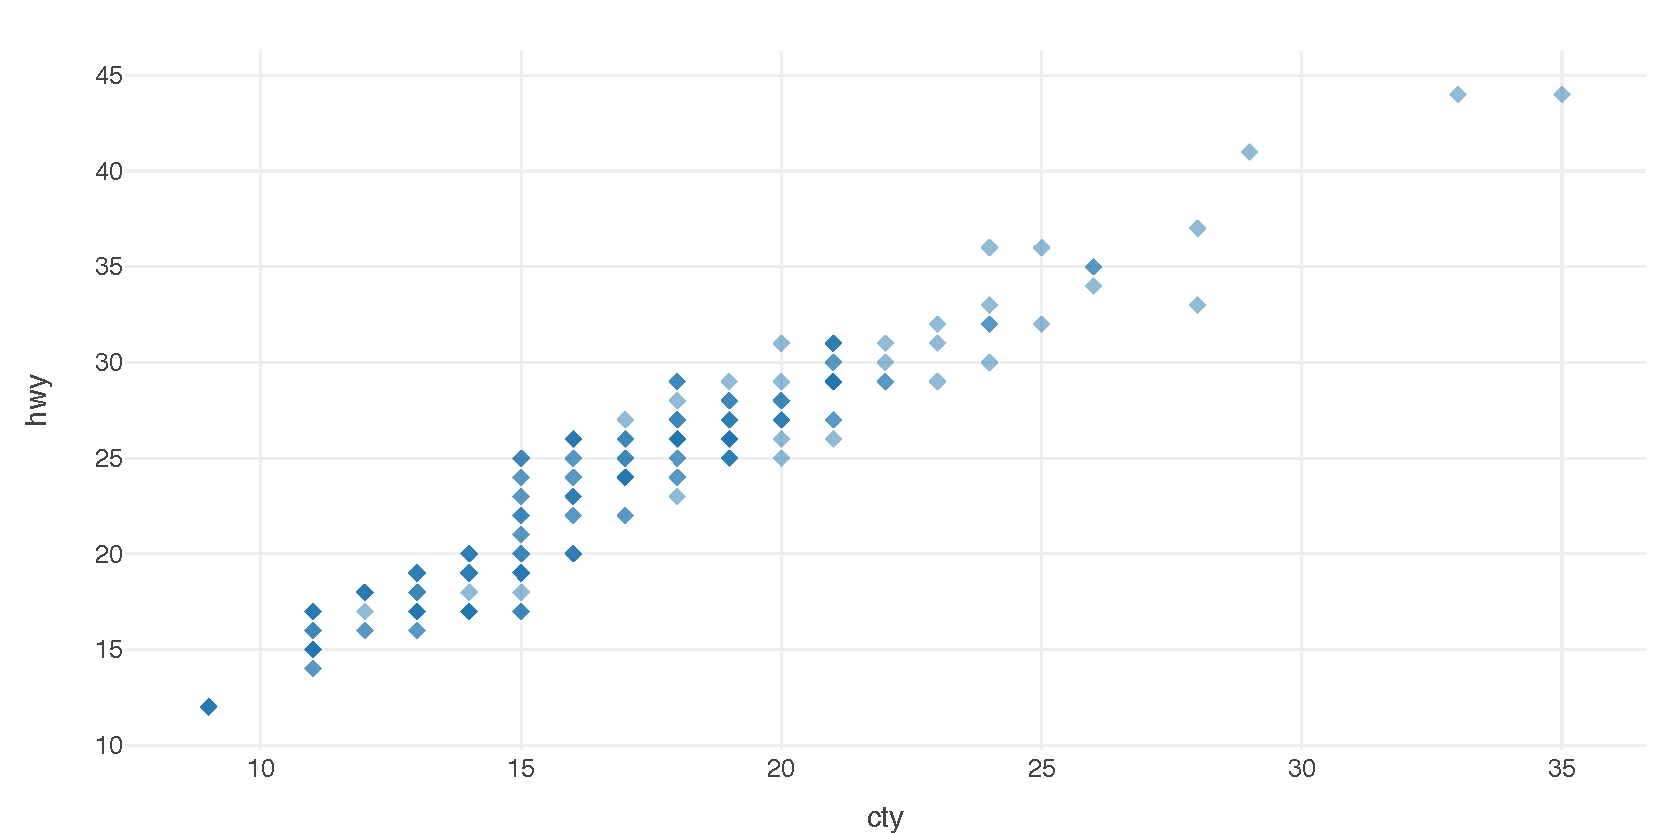
\includegraphics[width=\textwidth]{images/symbol-factor-manual} 

}

\caption{Setting a fixed symbol directly using \texttt{I()}.}\label{fig:symbol-factor-manual}
\end{figure}

If you'd like to see all the symbols available to \textbf{plotly}, as well as a method for supplying your own custom glyphs, see Chapter \ref{working-with-symbols}.

\hypertarget{marker-stroke}{%
\subsection{Stroke and span}\label{marker-stroke}}

\index{plot\_ly()@\texttt{plot\_ly()}!Special attributes!stroke@\texttt{stroke} / \texttt{strokes}}
\index{plot\_ly()@\texttt{plot\_ly()}!Special attributes!span@\texttt{span} / \texttt{spans}}

The \texttt{stroke} argument follows the same semantics as \texttt{color} and \texttt{symbol} when it comes to variable mappings and specifying visual ranges. Typically you don't want to map data values to \texttt{stroke}, you just want to specify a fixed outline color. For example, Figure \ref{fig:stroke-manual} modifies Figure \ref{fig:symbol-factor-manual} to simply add a black outline. By default, the \texttt{span}, or width of the stroke, is zero, you'll likely want to set the width to be around one pixel.

\begin{Shaded}
\begin{Highlighting}[]
\KeywordTok{plot_ly}\NormalTok{(mpg, }\DataTypeTok{x =} \OperatorTok{~}\NormalTok{cty, }\DataTypeTok{y =} \OperatorTok{~}\NormalTok{hwy, }\DataTypeTok{alpha =} \FloatTok{0.5}\NormalTok{) }\OperatorTok
\StringTok{  }\KeywordTok{add_markers}\NormalTok{(}\DataTypeTok{symbol =} \KeywordTok{I}\NormalTok{(}\DecValTok{18}\NormalTok{), }\DataTypeTok{stroke =} \KeywordTok{I}\NormalTok{(}\StringTok{"black"}\NormalTok{), }\DataTypeTok{span =} \KeywordTok{I}\NormalTok{(}\DecValTok{1}\NormalTok{))}
\end{Highlighting}
\end{Shaded}

\begin{figure}

{\centering 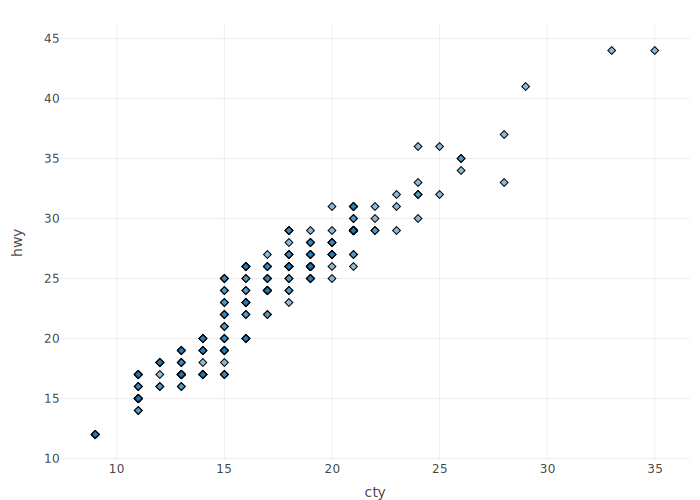
\includegraphics[width=\textwidth]{images/symbol-manual} 

}

\caption{Using \texttt{stroke} and \texttt{span} to control the outline color as well as the width of that outline.}\label{fig:stroke-manual}
\end{figure}

\hypertarget{marker-size}{%
\subsection{Size}\label{marker-size}}

\index{plot\_ly()@\texttt{plot\_ly()}!Special attributes!size@\texttt{size} / \texttt{sizes}}

For scatterplots, the \texttt{size} argument controls the area of markers (unless otherwise specified via \href{https://plot.ly/r/reference/\#scatter-marker-sizemode}{sizemode}), and \emph{must} be a numeric variable. The \texttt{sizes} argument controls the minimum and maximum size of circles, in pixels:

\begin{Shaded}
\begin{Highlighting}[]
\NormalTok{p <-}\StringTok{ }\KeywordTok{plot_ly}\NormalTok{(mpg, }\DataTypeTok{x =} \OperatorTok{~}\NormalTok{cty, }\DataTypeTok{y =} \OperatorTok{~}\NormalTok{hwy, }\DataTypeTok{alpha =} \FloatTok{0.3}\NormalTok{) }
\KeywordTok{subplot}\NormalTok{(}
  \KeywordTok{add_markers}\NormalTok{(p, }\DataTypeTok{size =} \OperatorTok{~}\NormalTok{cyl, }\DataTypeTok{name =} \StringTok{"default"}\NormalTok{),}
  \KeywordTok{add_markers}\NormalTok{(p, }\DataTypeTok{size =} \OperatorTok{~}\NormalTok{cyl, }\DataTypeTok{sizes =} \KeywordTok{c}\NormalTok{(}\DecValTok{1}\NormalTok{, }\DecValTok{500}\NormalTok{), }\DataTypeTok{name =} \StringTok{"custom"}\NormalTok{)}
\NormalTok{)}
\end{Highlighting}
\end{Shaded}

\begin{figure}

{\centering 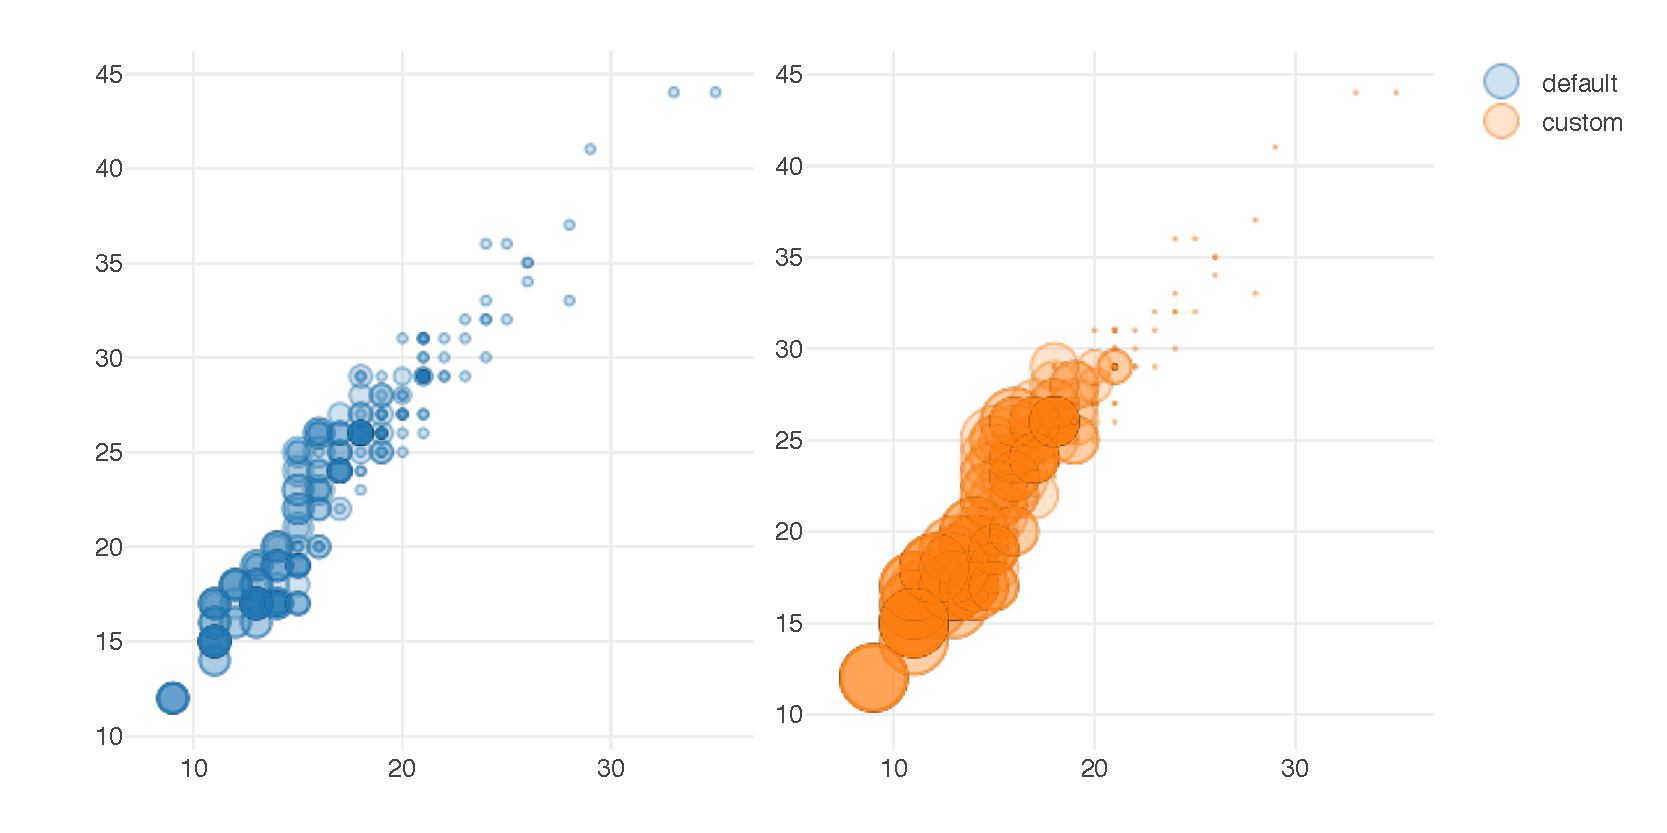
\includegraphics[width=\textwidth]{images/sizes} 

}

\caption{Controlling the size range via \texttt{sizes} (measured in pixels).}\label{fig:sizes}
\end{figure}

Similar to other arguments, \texttt{I()} can be used to specify the size directly. In the case of markers, \texttt{size} controls the \href{https://plot.ly/r/reference/\#scatter-marker-size}{\texttt{marker.size}} plotly.js attribute. Remember, you always have the option to set this attribute directly by doing something similar to Figure \ref{fig:sizes-manual}.

\begin{Shaded}
\begin{Highlighting}[]
\KeywordTok{plot_ly}\NormalTok{(mpg, }\DataTypeTok{x =} \OperatorTok{~}\NormalTok{cty, }\DataTypeTok{y =} \OperatorTok{~}\NormalTok{hwy, }\DataTypeTok{alpha =} \FloatTok{0.3}\NormalTok{, }\DataTypeTok{size =} \KeywordTok{I}\NormalTok{(}\DecValTok{30}\NormalTok{))}
\end{Highlighting}
\end{Shaded}

\begin{figure}

{\centering 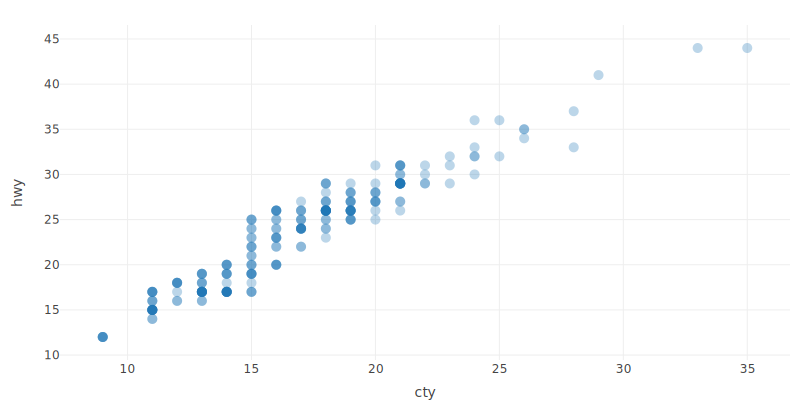
\includegraphics[width=\textwidth]{images/sizes-manual} 

}

\caption{Setting a fixed marker size directly using \texttt{marker.size}.}\label{fig:sizes-manual}
\end{figure}

\hypertarget{dot-plots}{%
\subsection{Dotplots \& error bars}\label{dot-plots}}

\index{Chart types!Dotplot}
\index{add\_trace()@\texttt{add\_trace()}!add\_markers()@\texttt{add\_markers()}!Error bars}

A dotplot is similar to a scatterplot, except instead of two numeric axes, one is categorical. The usual goal of a dotplot is to compare value(s) on a numerical scale over numerous categories. In this context, dotplots are preferable to pie charts since comparing position along a common scale is much easier than comparing angle or area \citep{graphical-perception, crowdsourcing-graphical-perception}. Furthermore, dotplots can be preferable to bar charts, especially when comparing values within a narrow range far away from 0 \citep{few-values}. Also, when presenting point estimates, and uncertainty associated with those estimates, bar charts tend to exaggerate the difference in point estimates, and lose focus on uncertainty \citep{messing}.

A popular application for dotplots (with error bars) is the so-called ``coefficient plot'' for visualizing the point estimates of coefficients and their standard error. The \texttt{coefplot()} function in the \textbf{coefplot} package \citep{coefplot} and the \texttt{ggcoef()} function in the \textbf{GGally} both produce coefficient plots for many types of model objects in R using \textbf{ggplot2}, which we can translate to plotly via \texttt{ggplotly()}. Since these packages use points and segments to draw the coefficient plots, the hover information is not the best, and it'd be better to use \href{https://plot.ly/r/reference/\#scatter-error_x}{error objects}. Figure \ref{fig:coefplot} uses the \texttt{tidy()} function from the \textbf{broom} package \citep{broom} to obtain a data frame with one row per model coefficient, and produce a coefficient plot with error bars along the x-axis.

\begin{Shaded}
\begin{Highlighting}[]
\CommentTok{# Fit a full-factorial linear model}
\NormalTok{m <-}\StringTok{ }\KeywordTok{lm}\NormalTok{(}
\NormalTok{  Sepal.Length }\OperatorTok{~}\StringTok{ }\NormalTok{Sepal.Width }\OperatorTok{*}\StringTok{ }\NormalTok{Petal.Length }\OperatorTok{*}\StringTok{ }\NormalTok{Petal.Width, }
  \DataTypeTok{data =}\NormalTok{ iris}
\NormalTok{)}

\CommentTok{# (1) get a tidy() data structure of covariate-level info }
\CommentTok{# (e.g., point estimate, standard error, etc)}
\CommentTok{# (2) make sure term column is a factor ordered by the estimate}
\CommentTok{# (3) plot estimate by term with an error bar for the standard error}
\NormalTok{broom}\OperatorTok{::}\KeywordTok{tidy}\NormalTok{(m) }\OperatorTok\StringTok{ }
\StringTok{  }\KeywordTok{mutate}\NormalTok{(}\DataTypeTok{term =}\NormalTok{ forcats}\OperatorTok{::}\KeywordTok{fct_reorder}\NormalTok{(term, estimate)) }\OperatorTok
\StringTok{  }\KeywordTok{plot_ly}\NormalTok{(}\DataTypeTok{x =} \OperatorTok{~}\NormalTok{estimate, }\DataTypeTok{y =} \OperatorTok{~}\NormalTok{term) }\OperatorTok
\StringTok{  }\KeywordTok{add_markers}\NormalTok{(}
    \DataTypeTok{error_x =} \OperatorTok{~}\KeywordTok{list}\NormalTok{(}\DataTypeTok{value =}\NormalTok{ std.error), }
    \DataTypeTok{color =} \KeywordTok{I}\NormalTok{(}\StringTok{"black"}\NormalTok{),}
    \DataTypeTok{hoverinfo =} \StringTok{"x"}
\NormalTok{  )}
\end{Highlighting}
\end{Shaded}

\begin{figure}

{\centering 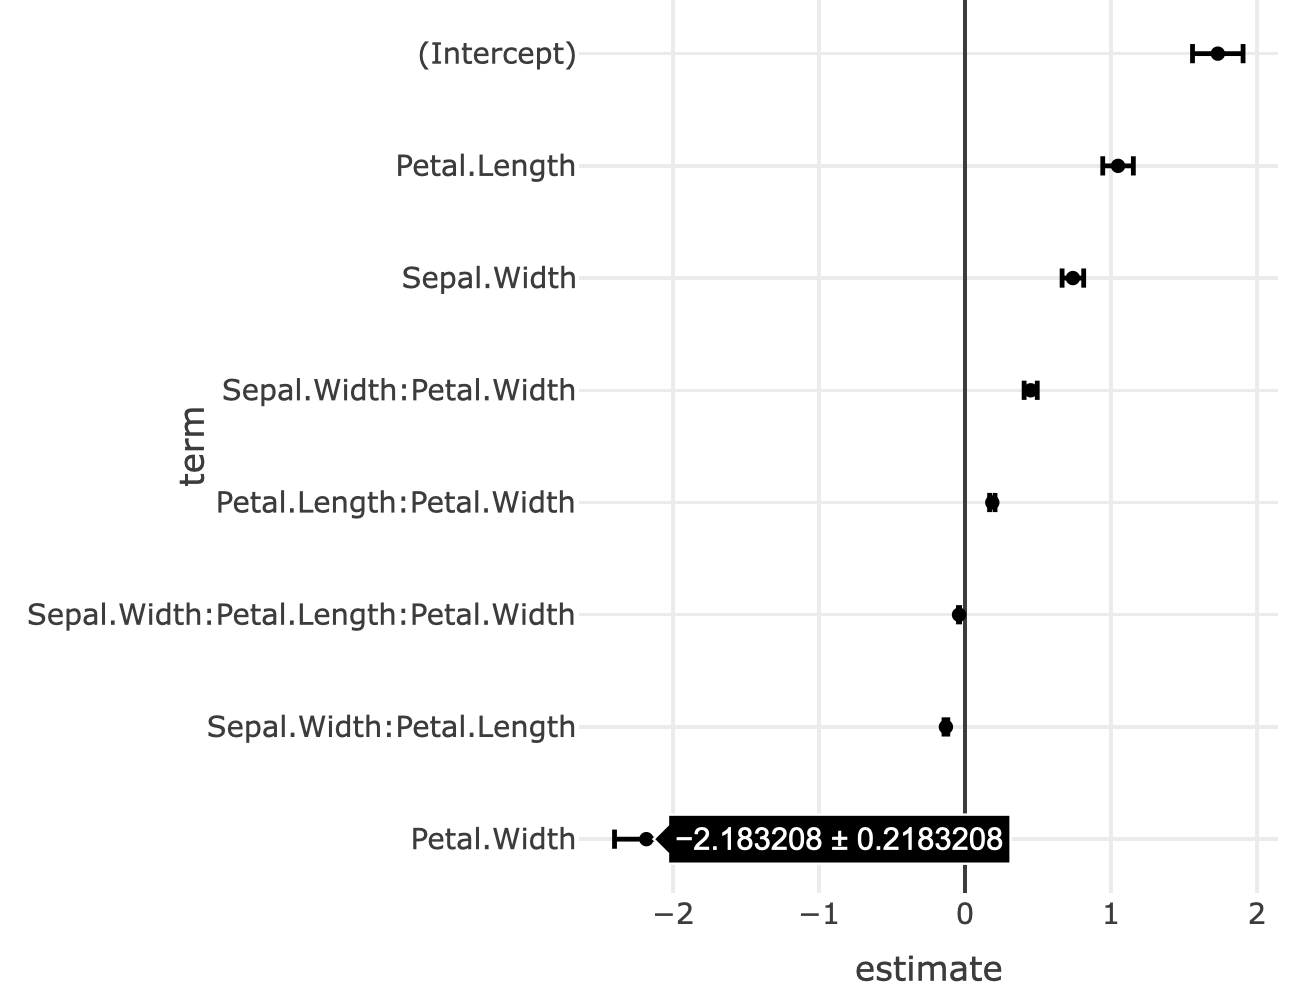
\includegraphics[width=\textwidth]{images/coefplot} 

}

\caption{A coefficient plot.}\label{fig:coefplot}
\end{figure}

\hypertarget{lines}{%
\section{Lines}\label{lines}}

\index{add\_trace()@\texttt{add\_trace()}!add\_lines()@\texttt{add\_lines()}}

Many of the same principles we learned about aesthetic mappings with respect to markers (Section \ref{markers}) also apply to lines.\footnote{At the time of writing, the plotly.js attributes \href{https://github.com/plotly/plotly.js/issues/147}{\texttt{line.width} and \texttt{line.color}} do not support multiple values, meaning a single line trace can only have one width/color in 2D line plot, and consequently numeric \texttt{color}/\texttt{size} mappings won't work. This isn't necessarily true for 3D paths/lines and there will likely be support these features for 2D paths/lines in WebGL in the near future.} Moreover, at the start of this chapter (namely Figure \ref{fig:scatter-lines}) we also learned how to use \textbf{dplyr}'s \texttt{group\_by()} to ensure there is at least one geometry (in this case, line) per group. We also learned the difference between \texttt{add\_paths()} and \texttt{add\_lines()} -- the former draws lines according to row ordering whereas the latter draw them according to \texttt{x}. In this chapter, we'll learn about \texttt{linetype}/\texttt{linetype}, an aesthetic that applies to lines and polygons. We'll also discuss some other important chart types that can be implemented with \texttt{add\_paths()}, \texttt{add\_lines()}, and \texttt{add\_segments()}.

\hypertarget{linetypes}{%
\subsection{Linetypes}\label{linetypes}}

\index{plot\_ly()@\texttt{plot\_ly()}!Special attributes!linetype@\texttt{linetype} / \texttt{linetypes}}

Generally speaking, it's hard to perceive more than 8 different colors/linetypes/symbols in a given plot, so sometimes we have to filter data to use these effectively. Here we use the \textbf{dplyr} package to find the top 5 cities in terms of average monthly sales (\texttt{top5}), then effectively filter the original data to contain just these cities via \texttt{semi\_join()}. As Figure \ref{fig:linetypes} demonstrates, once we have the data filtered, mapping city to \texttt{color} or \texttt{linetype} is trivial. The color palette can be altered via the \texttt{colors} argument, and follows the same rules as \protect\hyperlink{scatterplots}{scatterplots}. The linetype palette can be altered via the \texttt{linetypes} argument, and accepts R's \href{https://github.com/wch/r-source/blob/e5b21d0397c607883ff25cca379687b86933d730/src/library/graphics/man/par.Rd\#L726-L743}{\texttt{lty} values} or plotly.js \href{https://plot.ly/r/reference/\#scatter-line-dash}{dash values}.

\begin{Shaded}
\begin{Highlighting}[]
\KeywordTok{library}\NormalTok{(dplyr)}
\NormalTok{top5 <-}\StringTok{ }\NormalTok{txhousing }\OperatorTok
\StringTok{  }\KeywordTok{group_by}\NormalTok{(city) }\OperatorTok
\StringTok{  }\KeywordTok{summarise}\NormalTok{(}\DataTypeTok{m =} \KeywordTok{mean}\NormalTok{(sales, }\DataTypeTok{na.rm =} \OtherTok{TRUE}\NormalTok{)) }\OperatorTok
\StringTok{  }\KeywordTok{arrange}\NormalTok{(}\KeywordTok{desc}\NormalTok{(m)) }\OperatorTok
\StringTok{  }\KeywordTok{top_n}\NormalTok{(}\DecValTok{5}\NormalTok{)}

\NormalTok{tx5 <-}\StringTok{ }\KeywordTok{semi_join}\NormalTok{(txhousing, top5, }\DataTypeTok{by =} \StringTok{"city"}\NormalTok{)}

\KeywordTok{plot_ly}\NormalTok{(tx5, }\DataTypeTok{x =} \OperatorTok{~}\NormalTok{date, }\DataTypeTok{y =} \OperatorTok{~}\NormalTok{median) }\OperatorTok
\StringTok{  }\KeywordTok{add_lines}\NormalTok{(}\DataTypeTok{linetype =} \OperatorTok{~}\NormalTok{city)}
\end{Highlighting}
\end{Shaded}

\begin{figure}

{\centering 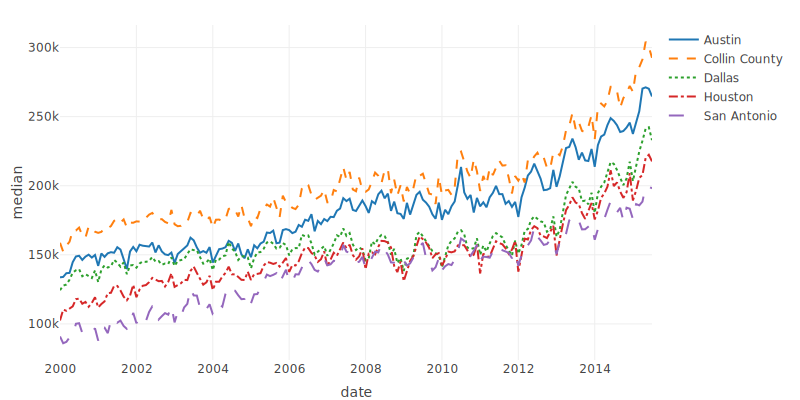
\includegraphics[width=\textwidth]{images/linetypes} 

}

\caption{Using \texttt{color} and/or \texttt{linetype} to differentiate groups of lines.}\label{fig:linetypes}
\end{figure}

If you'd like to control exactly which linetype is used to encode a particular data value, you can provide a named character vector, like in Figure \ref{fig:linetypes-manual}. Note that this is similar to how we provided a discrete colorscale manually for markers in Figure \ref{fig:color-discrete}.

\begin{Shaded}
\begin{Highlighting}[]
\NormalTok{ltys <-}\StringTok{ }\KeywordTok{c}\NormalTok{(}
  \DataTypeTok{Austin =} \StringTok{"dashdot"}\NormalTok{,}
  \StringTok{`}\DataTypeTok{Collin County}\StringTok{`}\NormalTok{ =}\StringTok{ "longdash"}\NormalTok{,}
  \DataTypeTok{Dallas =} \StringTok{"dash"}\NormalTok{,}
  \DataTypeTok{Houston =} \StringTok{"solid"}\NormalTok{,}
  \StringTok{`}\DataTypeTok{San Antonio}\StringTok{`}\NormalTok{ =}\StringTok{ "dot"}
\NormalTok{)}

\KeywordTok{plot_ly}\NormalTok{(tx5, }\DataTypeTok{x =} \OperatorTok{~}\NormalTok{date, }\DataTypeTok{y =} \OperatorTok{~}\NormalTok{median) }\OperatorTok
\StringTok{  }\KeywordTok{add_lines}\NormalTok{(}\DataTypeTok{linetype =} \OperatorTok{~}\NormalTok{city, }\DataTypeTok{linetypes =}\NormalTok{ ltys)}
\end{Highlighting}
\end{Shaded}

\begin{figure}

{\centering 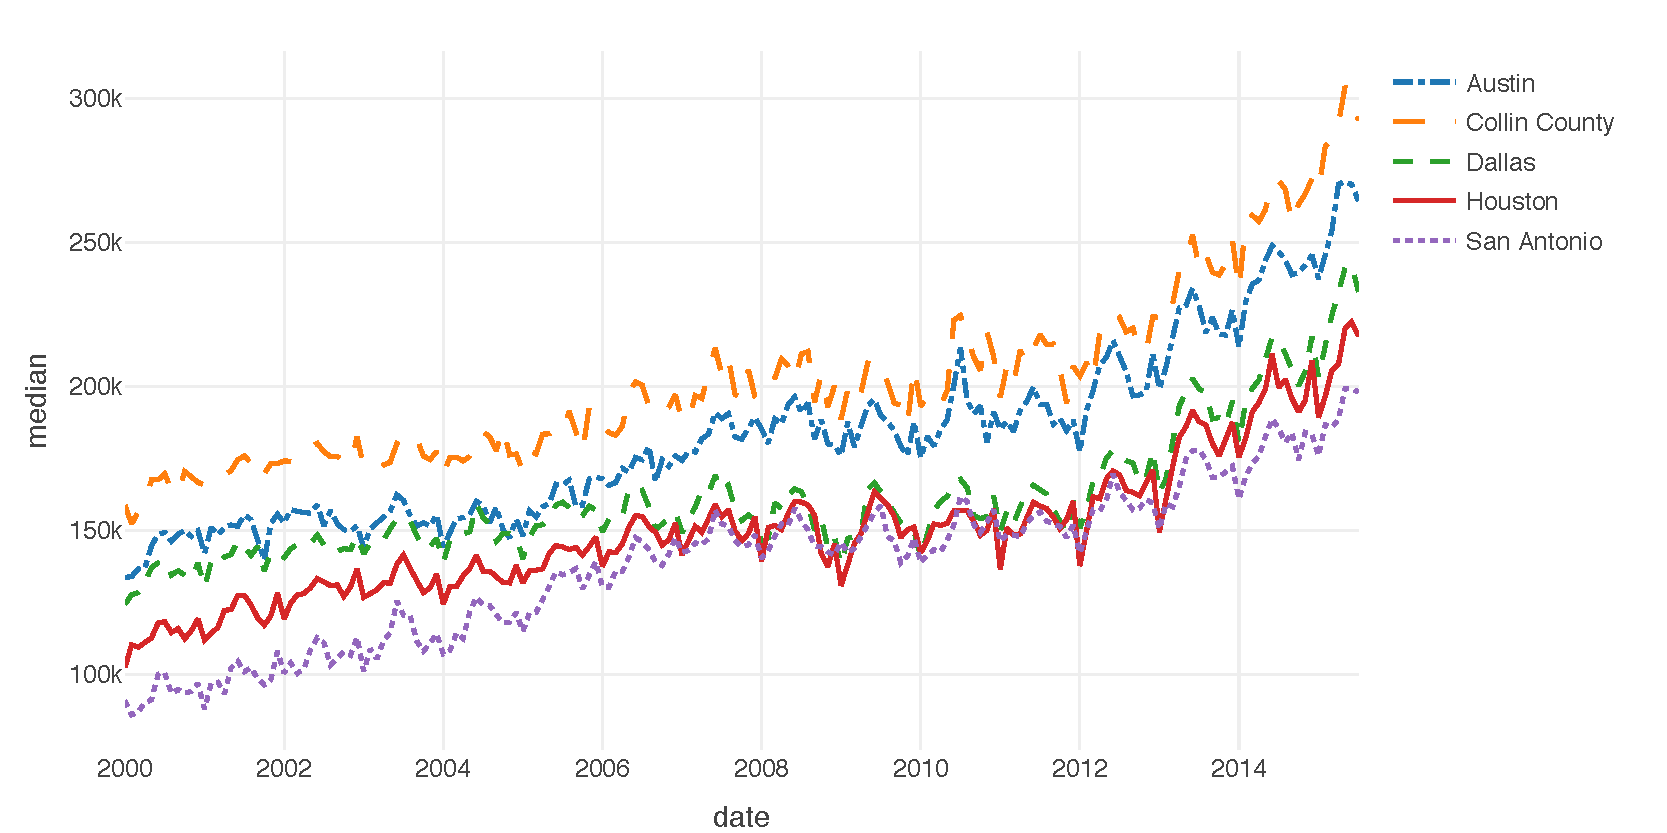
\includegraphics[width=\textwidth]{images/linetypes-manual} 

}

\caption{Providing a named character vector to linetypes in order to control exactly what linetype gets mapped to which city.}\label{fig:linetypes-manual}
\end{figure}

\hypertarget{segments}{%
\subsection{Segments}\label{segments}}

\index{add\_trace()@\texttt{add\_trace()}!add\_segments()@\texttt{add\_segments()}}

The \texttt{add\_segments()} function essentially provides a way to connect two points {[}(\texttt{x}, \texttt{y}) to (\texttt{xend}, \texttt{yend}){]} with a line. Segments form the building blocks for numerous useful chart types, including slopegraphs, dumbell charts, candlestick charts, and more. Slopegraphs and dumbell charts are useful for comparing numeric values across numerous categories. Candlestick charts are typically used for visualizing change in a financial asset over time.

Segments can also provide a useful alternative to \texttt{add\_bars()} (covered in Chapter \ref{bars-histograms}), especially for animations. In particular, Figure \ref{fig:profile-pyramid} of Section \ref{animation-support} shows how implement an animated population pyramid using segments instead of bars.

\hypertarget{slopegraph}{%
\subsubsection{Slopegraph}\label{slopegraph}}

\index{Chart types!Slopegraph}
\index{Editable charts!Annotations}
\index{add\_annotations()@\texttt{add\_annotations()}!Data coordinates}
\index{layout()@\texttt{layout()}!2D Axes}!range@\texttt{range}

\index{layout()@\texttt{layout()}!2D Axes!tickvals@\texttt{tickvals}}
\index{layout()@\texttt{layout()}!2D
Axes!ticktext@\texttt{ticktext}}
\index{layout()@\texttt{layout()}!2D Axes!zeroline@\texttt{zeroline}}
\index{layout()@\texttt{layout()}!2D Axes!showgrid@\texttt{showgrid}}
\index{layout()@\texttt{layout()}!2D Axes!showticks@\texttt{showticks}}
\index{layout()@\texttt{layout()}!2D Axes!showticklabels@\texttt{showticklabels}}
The slope graph, made popular by \citet{tufte2001}, is a great way to compare the change in a measurement across numerous groups. This change could be along either a discrete or a continuous axis. For a continuous axis, the slopegraph could be thought of as a decomposition of a line graph into multiple segments. The \textbf{slopegraph} R package provides a succinct interface for creating slopegraphs with base or \textbf{ggplot2} graphics and also some convenient data sets which we'll make use of here \citep{slopegraph}. Figure \ref{fig:slopegraph} recreates an example from \citet{tufte2001}, using the \texttt{gdp} data set from \textbf{slopegraph}, and demonstrates a common issue with labelling in slopegraphs -- it's easy to have overlapping labels when anchoring labels on data values. For that reason, this implementation leverages \textbf{plotly} ability to interactively edit annotation positions. See Chapter \ref{editing-views} for similar examples of `editing views'.

\begin{Shaded}
\begin{Highlighting}[]
\KeywordTok{data}\NormalTok{(gdp, }\DataTypeTok{package =} \StringTok{"slopegraph"}\NormalTok{)}
\NormalTok{gdp}\OperatorTok{$}\NormalTok{Country <-}\StringTok{ }\KeywordTok{row.names}\NormalTok{(gdp)}

\KeywordTok{plot_ly}\NormalTok{(gdp) }\OperatorTok
\StringTok{  }\KeywordTok{add_segments}\NormalTok{(}
    \DataTypeTok{x =} \DecValTok{1}\NormalTok{, }\DataTypeTok{xend =} \DecValTok{2}\NormalTok{,}
    \DataTypeTok{y =} \OperatorTok{~}\NormalTok{Year1970, }\DataTypeTok{yend =} \OperatorTok{~}\NormalTok{Year1979,}
    \DataTypeTok{color =} \KeywordTok{I}\NormalTok{(}\StringTok{"gray90"}\NormalTok{)}
\NormalTok{  ) }\OperatorTok
\StringTok{  }\KeywordTok{add_annotations}\NormalTok{(}
    \DataTypeTok{x =} \DecValTok{1}\NormalTok{, }\DataTypeTok{y =} \OperatorTok{~}\NormalTok{Year1970, }
    \DataTypeTok{text =} \OperatorTok{~}\KeywordTok{paste}\NormalTok{(Country, }\StringTok{"  "}\NormalTok{, Year1970), }
    \DataTypeTok{xanchor =} \StringTok{"right"}\NormalTok{, }\DataTypeTok{showarrow =} \OtherTok{FALSE}
\NormalTok{  ) }\OperatorTok
\StringTok{  }\KeywordTok{add_annotations}\NormalTok{(}
    \DataTypeTok{x =} \DecValTok{2}\NormalTok{, }\DataTypeTok{y =} \OperatorTok{~}\NormalTok{Year1979, }
    \DataTypeTok{text =} \OperatorTok{~}\KeywordTok{paste}\NormalTok{(Year1979, }\StringTok{"  "}\NormalTok{, Country),}
    \DataTypeTok{xanchor =} \StringTok{"left"}\NormalTok{, }\DataTypeTok{showarrow =} \OtherTok{FALSE}
\NormalTok{  ) }\OperatorTok
\StringTok{  }\KeywordTok{layout}\NormalTok{(}
    \DataTypeTok{title =} \StringTok{"Current Receipts of Govermnent as a Percentage of GDP"}\NormalTok{,}
    \DataTypeTok{showlegend =} \OtherTok{FALSE}\NormalTok{,}
    \DataTypeTok{xaxis =} \KeywordTok{list}\NormalTok{(}
      \DataTypeTok{range =} \KeywordTok{c}\NormalTok{(}\DecValTok{0}\NormalTok{, }\DecValTok{3}\NormalTok{),}
      \DataTypeTok{ticktext =} \KeywordTok{c}\NormalTok{(}\StringTok{"1970"}\NormalTok{, }\StringTok{"1979"}\NormalTok{),}
      \DataTypeTok{tickvals =} \KeywordTok{c}\NormalTok{(}\DecValTok{1}\NormalTok{, }\DecValTok{2}\NormalTok{),}
      \DataTypeTok{zeroline =} \OtherTok{FALSE}
\NormalTok{    ),}
    \DataTypeTok{yaxis =} \KeywordTok{list}\NormalTok{(}
      \DataTypeTok{title =} \StringTok{""}\NormalTok{,}
      \DataTypeTok{showgrid =} \OtherTok{FALSE}\NormalTok{,}
      \DataTypeTok{showticks =} \OtherTok{FALSE}\NormalTok{,}
      \DataTypeTok{showticklabels =} \OtherTok{FALSE}
\NormalTok{    )}
\NormalTok{  ) }\OperatorTok\StringTok{ }
\StringTok{  }\KeywordTok{config}\NormalTok{(}\DataTypeTok{edits =} \KeywordTok{list}\NormalTok{(}\DataTypeTok{annotationPosition =} \OtherTok{TRUE}\NormalTok{))}
\end{Highlighting}
\end{Shaded}

\begin{figure}

{\centering 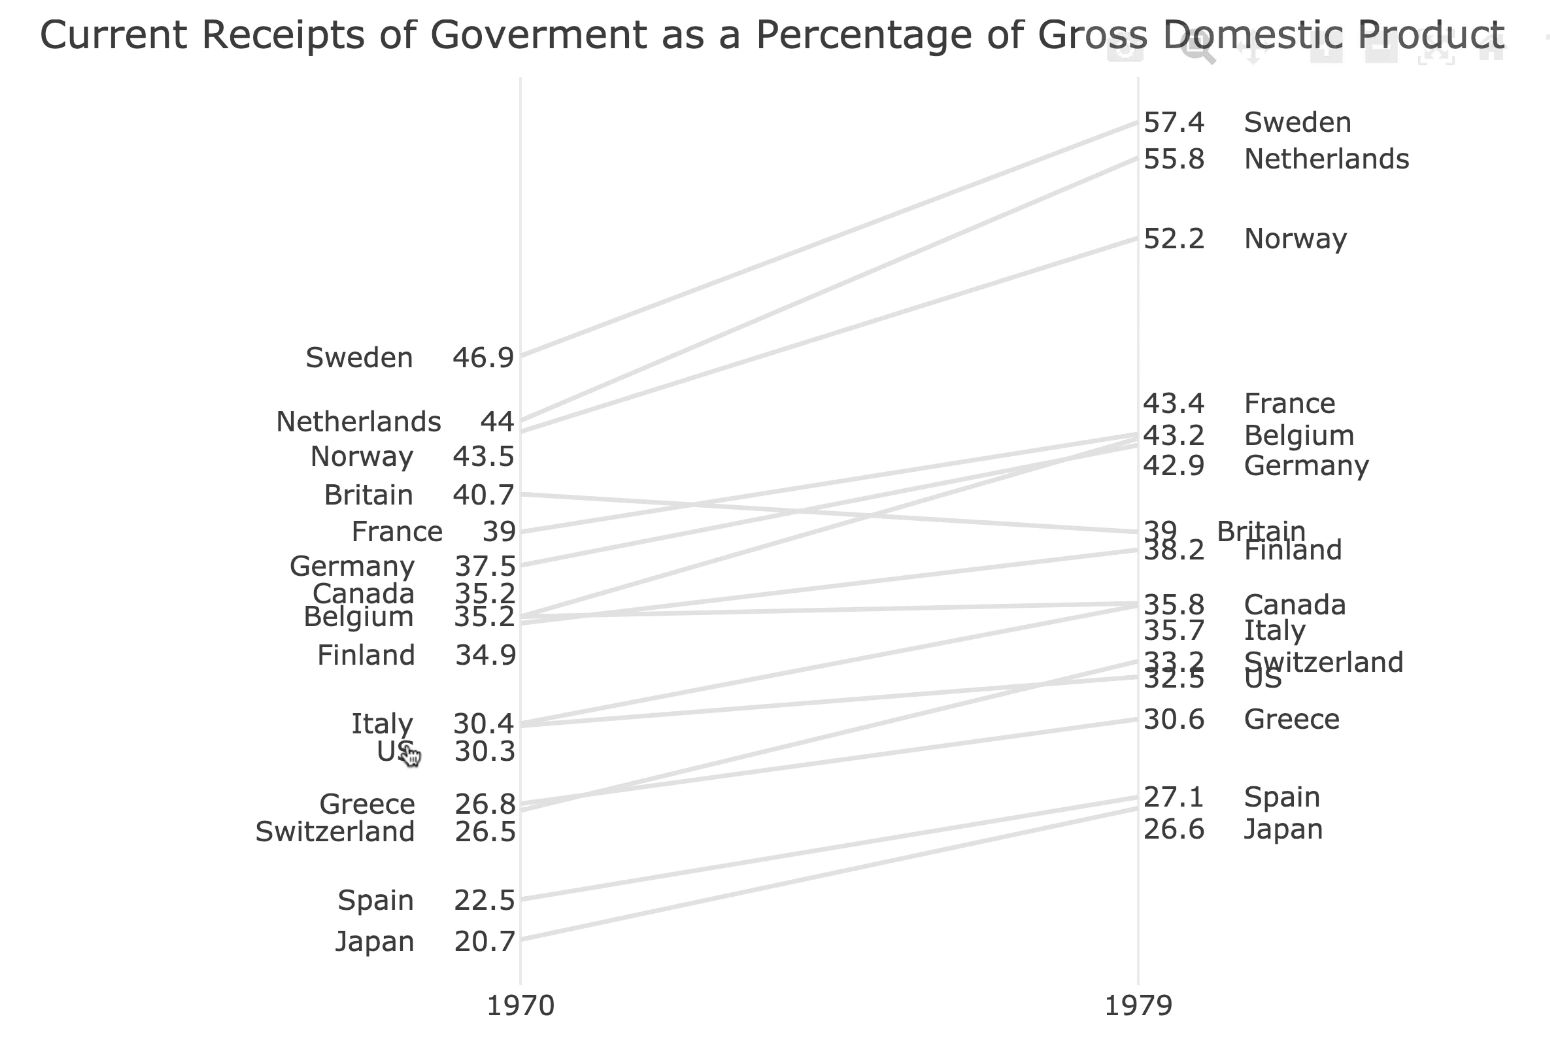
\includegraphics[width=\textwidth]{vimeo-images/327585190/final} 

}

\caption{Interactively editing the label positioning in a slopegraph. For a video demonstration of the interactive, see \url{https://bit.ly/Slopegraph}. For the interactive, see \url{https://plotly-r.com/interactives/slopegraph.html}}\label{fig:slopegraph}
\end{figure}

\hypertarget{dumbell}{%
\subsubsection{Dumbell}\label{dumbell}}

\index{Chart types!Dumbell}

So called dumbell charts are similar in concept to slope graphs, but not quite as general. They are typically used to compare two different classes of numeric values across numerous groups. Figure \ref{fig:dumbell} uses the dumbell approach to show average miles per gallon city and highway for different car models. With a dumbell chart, it's always a good idea to order the categories by a sensible metric -- for Figure \ref{fig:dumbell}, the categories are ordered by the city miles per gallon.

\begin{Shaded}
\begin{Highlighting}[]
\NormalTok{mpg }\OperatorTok
\StringTok{  }\KeywordTok{group_by}\NormalTok{(model) }\OperatorTok
\StringTok{  }\KeywordTok{summarise}\NormalTok{(}\DataTypeTok{c =} \KeywordTok{mean}\NormalTok{(cty), }\DataTypeTok{h =} \KeywordTok{mean}\NormalTok{(hwy)) }\OperatorTok
\StringTok{  }\KeywordTok{mutate}\NormalTok{(}\DataTypeTok{model =}\NormalTok{ forcats}\OperatorTok{::}\KeywordTok{fct_reorder}\NormalTok{(model, c)) }\OperatorTok
\StringTok{  }\KeywordTok{plot_ly}\NormalTok{() }\OperatorTok
\StringTok{  }\KeywordTok{add_segments}\NormalTok{(}
    \DataTypeTok{x =} \OperatorTok{~}\NormalTok{c, }\DataTypeTok{y =} \OperatorTok{~}\NormalTok{model,}
    \DataTypeTok{xend =} \OperatorTok{~}\NormalTok{h, }\DataTypeTok{yend =} \OperatorTok{~}\NormalTok{model, }
    \DataTypeTok{color =} \KeywordTok{I}\NormalTok{(}\StringTok{"gray"}\NormalTok{), }\DataTypeTok{showlegend =} \OtherTok{FALSE}
\NormalTok{  ) }\OperatorTok
\StringTok{  }\KeywordTok{add_markers}\NormalTok{(}
    \DataTypeTok{x =} \OperatorTok{~}\NormalTok{c, }\DataTypeTok{y =} \OperatorTok{~}\NormalTok{model, }
    \DataTypeTok{color =} \KeywordTok{I}\NormalTok{(}\StringTok{"blue"}\NormalTok{), }
    \DataTypeTok{name =} \StringTok{"mpg city"}
\NormalTok{  ) }\OperatorTok
\StringTok{  }\KeywordTok{add_markers}\NormalTok{(}
    \DataTypeTok{x =} \OperatorTok{~}\NormalTok{h, }\DataTypeTok{y =} \OperatorTok{~}\NormalTok{model, }
    \DataTypeTok{color =} \KeywordTok{I}\NormalTok{(}\StringTok{"red"}\NormalTok{),}
    \DataTypeTok{name  =} \StringTok{"mpg highway"}
\NormalTok{  ) }\OperatorTok
\StringTok{  }\KeywordTok{layout}\NormalTok{(}\DataTypeTok{xaxis =} \KeywordTok{list}\NormalTok{(}\DataTypeTok{title =} \StringTok{"Miles per gallon"}\NormalTok{))}
\end{Highlighting}
\end{Shaded}

\begin{figure}

{\centering 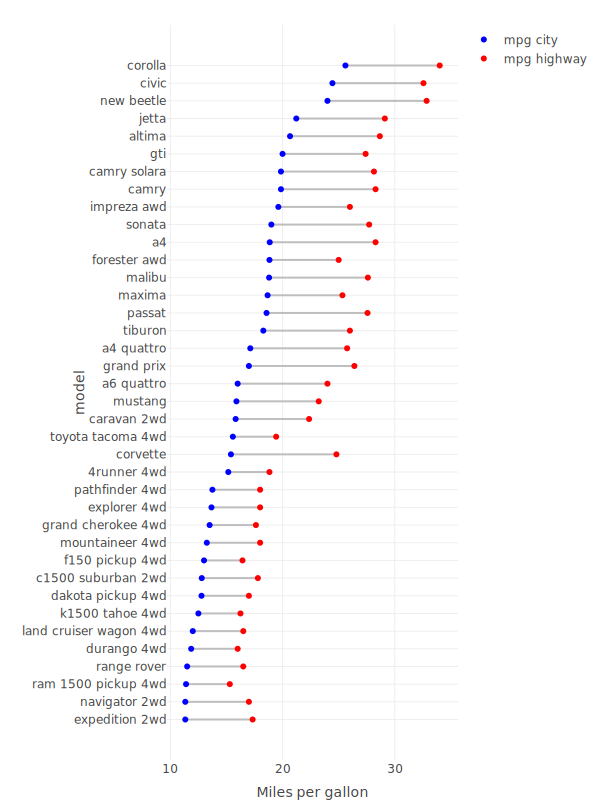
\includegraphics[width=\textwidth]{images/dumbell} 

}

\caption{A dumbell chart of mile per gallon city vs highway by model of car.}\label{fig:dumbell}
\end{figure}

\hypertarget{candlestick}{%
\subsubsection{Candlestick}\label{candlestick}}

\index{Chart types!Candlestick}

Figure \ref{fig:candlestick} uses the \textbf{quantmod} package \citep{quantmod} to obtain stock price data for Microsoft and plots two segments for each day: one to encode the opening/closing values, and one to encode the daily high/low.

\begin{Shaded}
\begin{Highlighting}[]
\KeywordTok{library}\NormalTok{(quantmod)}
\NormalTok{msft <-}\StringTok{ }\KeywordTok{getSymbols}\NormalTok{(}\StringTok{"MSFT"}\NormalTok{, }\DataTypeTok{auto.assign =}\NormalTok{ F)}
\NormalTok{dat <-}\StringTok{ }\KeywordTok{as.data.frame}\NormalTok{(msft)}
\NormalTok{dat}\OperatorTok{$}\NormalTok{date <-}\StringTok{ }\KeywordTok{index}\NormalTok{(msft)}
\NormalTok{dat <-}\StringTok{ }\KeywordTok{subset}\NormalTok{(dat, date }\OperatorTok{>=}\StringTok{ "2016-01-01"}\NormalTok{)}

\KeywordTok{names}\NormalTok{(dat) <-}\StringTok{ }\KeywordTok{sub}\NormalTok{(}\StringTok{"^MSFT}\CharTok{\textbackslash{}\textbackslash{}}\StringTok{."}\NormalTok{, }\StringTok{""}\NormalTok{, }\KeywordTok{names}\NormalTok{(dat))}

\KeywordTok{plot_ly}\NormalTok{(dat, }\DataTypeTok{x =} \OperatorTok{~}\NormalTok{date, }\DataTypeTok{xend =} \OperatorTok{~}\NormalTok{date, }\DataTypeTok{color =} \OperatorTok{~}\NormalTok{Close }\OperatorTok{>}\StringTok{ }\NormalTok{Open, }
        \DataTypeTok{colors =} \KeywordTok{c}\NormalTok{(}\StringTok{"red"}\NormalTok{, }\StringTok{"forestgreen"}\NormalTok{), }\DataTypeTok{hoverinfo =} \StringTok{"none"}\NormalTok{) }\OperatorTok
\StringTok{  }\KeywordTok{add_segments}\NormalTok{(}\DataTypeTok{y =} \OperatorTok{~}\NormalTok{Low, }\DataTypeTok{yend =} \OperatorTok{~}\NormalTok{High, }\DataTypeTok{size =} \KeywordTok{I}\NormalTok{(}\DecValTok{1}\NormalTok{)) }\OperatorTok
\StringTok{  }\KeywordTok{add_segments}\NormalTok{(}\DataTypeTok{y =} \OperatorTok{~}\NormalTok{Open, }\DataTypeTok{yend =} \OperatorTok{~}\NormalTok{Close, }\DataTypeTok{size =} \KeywordTok{I}\NormalTok{(}\DecValTok{3}\NormalTok{)) }\OperatorTok
\StringTok{  }\KeywordTok{layout}\NormalTok{(}\DataTypeTok{showlegend =} \OtherTok{FALSE}\NormalTok{, }\DataTypeTok{yaxis =} \KeywordTok{list}\NormalTok{(}\DataTypeTok{title =} \StringTok{"Price"}\NormalTok{)) }\OperatorTok
\StringTok{  }\KeywordTok{rangeslider}\NormalTok{()}
\end{Highlighting}
\end{Shaded}

\begin{figure}

{\centering 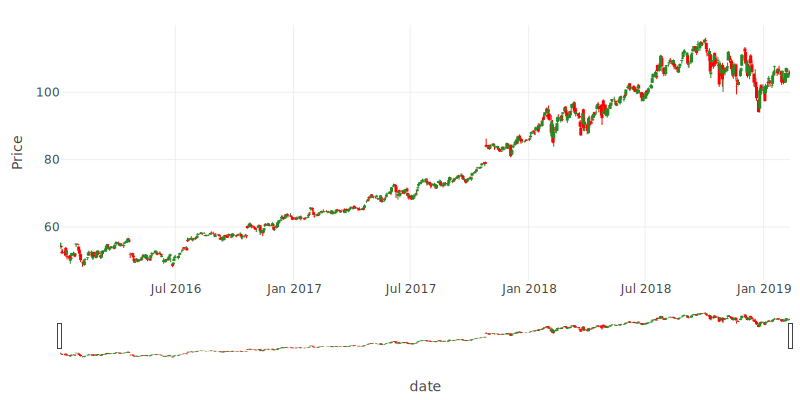
\includegraphics[width=\textwidth]{images/candlestick} 

}

\caption{A candlestick chart built out of segments}\label{fig:candlestick}
\end{figure}

\hypertarget{density-plots}{%
\subsection{Density plots}\label{density-plots}}

\index{Kernel density estimation!density()@\texttt{density()}}

In Chapter \ref{bars-histograms}, we leverage a number of algorithms in R for computing the ``optimal'' number of bins for a histogram, via \texttt{hist()}, and routing those results to \texttt{add\_bars()}. We can leverage the \texttt{density()} function for computing kernel density estimates in a similar way, and route the results to \texttt{add\_lines()}, as is done in Figure \ref{fig:densities}.

\begin{Shaded}
\begin{Highlighting}[]
\NormalTok{kerns <-}\StringTok{ }\KeywordTok{c}\NormalTok{(}\StringTok{"gaussian"}\NormalTok{, }\StringTok{"epanechnikov"}\NormalTok{, }\StringTok{"rectangular"}\NormalTok{, }
          \StringTok{"triangular"}\NormalTok{, }\StringTok{"biweight"}\NormalTok{, }\StringTok{"cosine"}\NormalTok{, }\StringTok{"optcosine"}\NormalTok{)}
\NormalTok{p <-}\StringTok{ }\KeywordTok{plot_ly}\NormalTok{()}
\ControlFlowTok{for}\NormalTok{ (k }\ControlFlowTok{in}\NormalTok{ kerns) \{}
\NormalTok{  d <-}\StringTok{ }\KeywordTok{density}\NormalTok{(economics}\OperatorTok{$}\NormalTok{pce, }\DataTypeTok{kernel =}\NormalTok{ k, }\DataTypeTok{na.rm =} \OtherTok{TRUE}\NormalTok{)}
\NormalTok{  p <-}\StringTok{ }\KeywordTok{add_lines}\NormalTok{(p, }\DataTypeTok{x =}\NormalTok{ d}\OperatorTok{$}\NormalTok{x, }\DataTypeTok{y =}\NormalTok{ d}\OperatorTok{$}\NormalTok{y, }\DataTypeTok{name =}\NormalTok{ k)}
\NormalTok{\}}
\NormalTok{p}
\end{Highlighting}
\end{Shaded}

\begin{figure}

{\centering 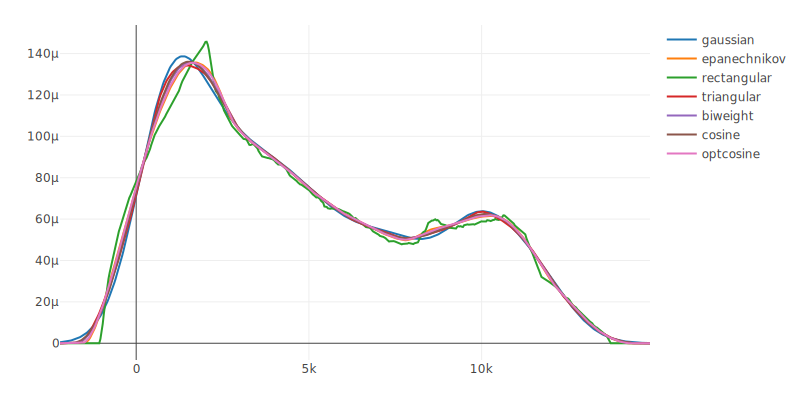
\includegraphics[width=\textwidth]{images/densities} 

}

\caption{Various kernel density estimates.}\label{fig:densities}
\end{figure}

\hypertarget{parallel-coordinates}{%
\subsection{Parallel Coordinates}\label{parallel-coordinates}}

\index{Chart types!Parallel coordinates}

One very useful, but often overlooked, visualization technique is the parallel coordinates plot. Parallel coordinates provide a way to compare values along a common (or non-aligned) positional scale(s) -- the most basic of all perceptual tasks -- in more than 3 dimensions \citep{graphical-perception}. Usually each line represents every measurement for a given row (or observation) in a data set. It's true that plotly.js provides a trace type, parcoords, specifically for parallel coordinates that offers desirable interactive capabilities (e.g., highlighting and reordering of axes).\footnote{See \url{https://plot.ly/r/parallel-coordinates-plot/} for some interactive examples}. However, it can also be useful learn how to use \texttt{add\_lines()} to implement parallel coordinates as it can offer more flexibility and control over the axis scales.

When measurements are on very different scales, some care must be taken, and variables must transformed to be put on a common scale. As Figure \ref{fig:pcp-common} shows, even when variables are measured on a similar scale, it can still be informative to transform variables in different ways.

\begin{Shaded}
\begin{Highlighting}[]
\NormalTok{iris}\OperatorTok{$}\NormalTok{obs <-}\StringTok{ }\KeywordTok{seq_len}\NormalTok{(}\KeywordTok{nrow}\NormalTok{(iris))}
\NormalTok{iris_pcp <-}\StringTok{ }\ControlFlowTok{function}\NormalTok{(}\DataTypeTok{transform =}\NormalTok{ identity) \{}
\NormalTok{  iris[] <-}\StringTok{ }\NormalTok{purrr}\OperatorTok{::}\KeywordTok{map_if}\NormalTok{(iris, is.numeric, transform)}
\NormalTok{  tidyr}\OperatorTok{::}\KeywordTok{gather}\NormalTok{(iris, variable, value, }\OperatorTok{-}\NormalTok{Species, }\OperatorTok{-}\NormalTok{obs) }\OperatorTok\StringTok{ }
\StringTok{    }\KeywordTok{group_by}\NormalTok{(obs) }\OperatorTok\StringTok{ }
\StringTok{    }\KeywordTok{plot_ly}\NormalTok{(}\DataTypeTok{x =} \OperatorTok{~}\NormalTok{variable, }\DataTypeTok{y =} \OperatorTok{~}\NormalTok{value, }\DataTypeTok{color =} \OperatorTok{~}\NormalTok{Species) }\OperatorTok\StringTok{ }
\StringTok{    }\KeywordTok{add_lines}\NormalTok{(}\DataTypeTok{alpha =} \FloatTok{0.3}\NormalTok{)}
\NormalTok{\}}
\KeywordTok{subplot}\NormalTok{(}
  \KeywordTok{iris_pcp}\NormalTok{(), }
  \KeywordTok{iris_pcp}\NormalTok{(scale),}
  \KeywordTok{iris_pcp}\NormalTok{(scales}\OperatorTok{::}\NormalTok{rescale),}
  \DataTypeTok{nrows =} \DecValTok{3}\NormalTok{, }\DataTypeTok{shareX =} \OtherTok{TRUE}
\NormalTok{) }\OperatorTok\StringTok{ }\KeywordTok{hide_legend}\NormalTok{()}
\end{Highlighting}
\end{Shaded}

\begin{figure}

{\centering 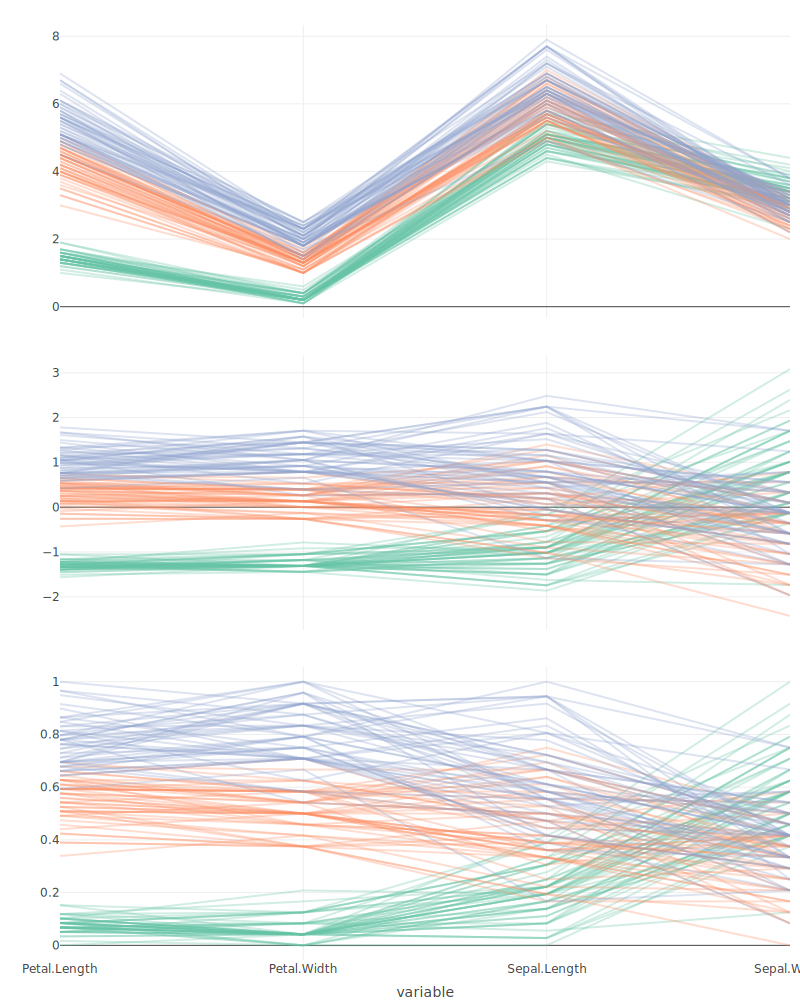
\includegraphics[width=\textwidth]{images/pcp-common} 

}

\caption{Parallel coordinates plots of the Iris dataset. The top panel shows all variables on a common scale. The middle panel scales each variable to have mean of 0 and standard deviation of 1. In the bottom panel, each variable is scaled to have a minimum of 0 and a maximum of 1.}\label{fig:pcp-common}
\end{figure}

It is also worth noting that the \textbf{GGally} offers a \texttt{ggparcoord()} function which creates parallel coordinate plots via \textbf{ggplot2}, which we can convert to plotly via \texttt{ggplotly()}. Thanks to the \protect\hyperlink{linking-views-without-shiny}{linked highlighting} framework, parallel coordinates created in this way could be linked to lower dimensional (but sometimes higher resolution) graphics of related data to guide multi-variate data exploration. The \textbf{pedestrians} package provides some examples of linking parallel coordinates to other views such as a grand tour for exposing unusual features in a high-dimensional space \citep{pedestrians}.

\hypertarget{polygons}{%
\section{Polygons}\label{polygons}}

\index{add\_trace()@\texttt{add\_trace()}!add\_polygons()@\texttt{add\_polygons()}}

\index{layout()@\texttt{layout()}!2D Axes!scaleanchor@\texttt{scaleanchor}}
The \texttt{add\_polygons()} function is essentially equivalent to \texttt{add\_paths()} with the \href{https://plot.ly/r/reference/\#scatter-fill}{fill} attribute set to ``toself''. Polygons form the basis for other, higher-level scatter-based layers (e.g., \texttt{add\_ribbons()} and \texttt{add\_sf()}) that don't have a dedicated plotly.js trace type. Polygons can be use to draw many things, but perhaps the most familiar application where you \emph{might} want to use \texttt{add\_polygons()} is to draw geo-spatial objects. If and when you use \texttt{add\_polygons()} to draw a map, make sure you fix the aspect ratio (e.g., \href{https://plot.ly/r/reference/\#layout-xaxis-scaleanchor}{\texttt{xaxis.scaleanchor}}) and also consider using \texttt{plotly\_empty()} over \texttt{plot\_ly()} to hide axis labels, ticks, and the background grid. On the other hand, Section \ref{maps-custom} shows you how to make a custom maps using the \textbf{sf} package and \texttt{add\_sf()}, which is a bit of work to get started, but is absolutely worth the investment.

\begin{Shaded}
\begin{Highlighting}[]
\NormalTok{base <-}\StringTok{ }\KeywordTok{map_data}\NormalTok{(}\StringTok{"world"}\NormalTok{, }\StringTok{"canada"}\NormalTok{) }\OperatorTok
\StringTok{  }\KeywordTok{group_by}\NormalTok{(group) }\OperatorTok
\StringTok{  }\KeywordTok{plotly_empty}\NormalTok{(}\DataTypeTok{x =} \OperatorTok{~}\NormalTok{long, }\DataTypeTok{y =} \OperatorTok{~}\NormalTok{lat, }\DataTypeTok{alpha =} \FloatTok{0.2}\NormalTok{) }\OperatorTok
\StringTok{  }\KeywordTok{layout}\NormalTok{(}\DataTypeTok{showlegend =} \OtherTok{FALSE}\NormalTok{, }\DataTypeTok{xaxis =} \KeywordTok{list}\NormalTok{(}\DataTypeTok{scaleanchor =} \StringTok{"y"}\NormalTok{))}
  
\NormalTok{base }\OperatorTok
\StringTok{  }\KeywordTok{add_polygons}\NormalTok{(}\DataTypeTok{hoverinfo =} \StringTok{"none"}\NormalTok{, }\DataTypeTok{color =} \KeywordTok{I}\NormalTok{(}\StringTok{"black"}\NormalTok{)) }\OperatorTok
\StringTok{  }\KeywordTok{add_markers}\NormalTok{(}\DataTypeTok{text =} \OperatorTok{~}\KeywordTok{paste}\NormalTok{(name, }\StringTok{"<br />"}\NormalTok{, pop), }\DataTypeTok{hoverinfo =} \StringTok{"text"}\NormalTok{, }
              \DataTypeTok{color =} \KeywordTok{I}\NormalTok{(}\StringTok{"red"}\NormalTok{), }\DataTypeTok{data =}\NormalTok{ maps}\OperatorTok{::}\NormalTok{canada.cities)}
\end{Highlighting}
\end{Shaded}

\begin{figure}

{\centering 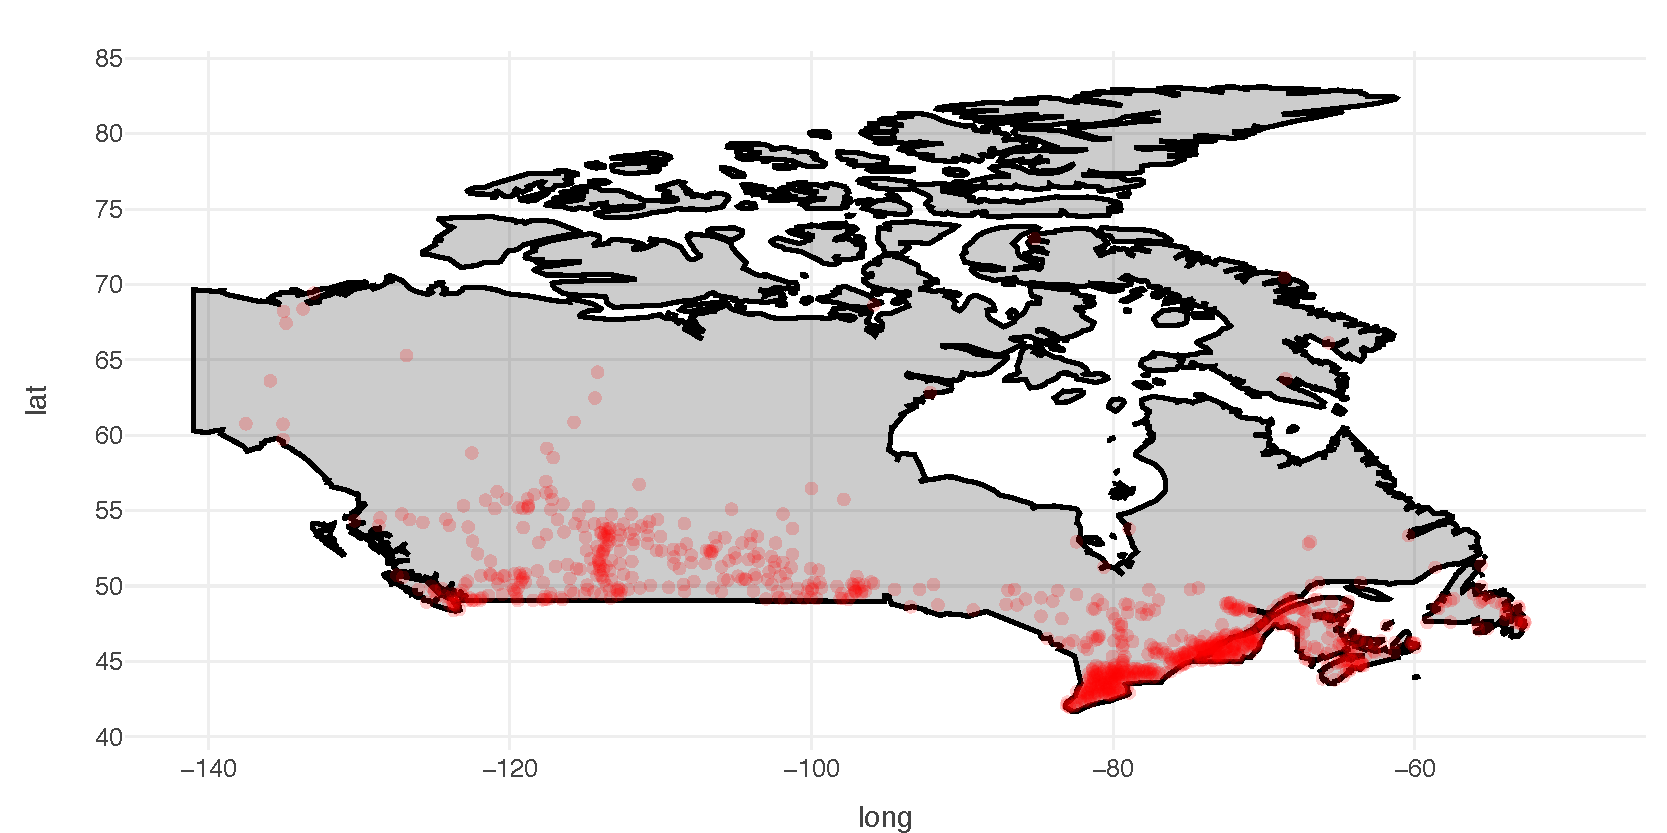
\includegraphics[width=\textwidth]{images/map-canada} 

}

\caption{Using \texttt{add\_polygons()} to make a map of Canada and major Canadian cities via data provided by the \textbf{maps} package.}\label{fig:map-canada}
\end{figure}

As discussion surrounding Figure \ref{fig:split-color} points out, scatter-based polygon layers (i.e., \texttt{add\_polygons()}, \texttt{add\_ribbons()}, etc) render all the polygons using one plotly.js trace by default. This approach is computationally efficient, but it's not always desirable (e.g., can't have multiple fills per trace, interactivity is relatively limited). To work around the limitations, consider using \texttt{split} (or \texttt{color} with a discrete variable) to split the polygon data into multiple traces. Figure \ref{fig:map-canada-split} demonstrates using \texttt{split} which will impose plotly.js' colorway to each trace (i.e., subregion) and leverage \texttt{hoveron} to generate one tooltip per sub-region.

\begin{Shaded}
\begin{Highlighting}[]
\KeywordTok{add_polygons}\NormalTok{(base, }\DataTypeTok{split =} \OperatorTok{~}\NormalTok{subregion, }\DataTypeTok{hoveron =} \StringTok{"fills"}\NormalTok{)}
\end{Highlighting}
\end{Shaded}

\begin{figure}

{\centering 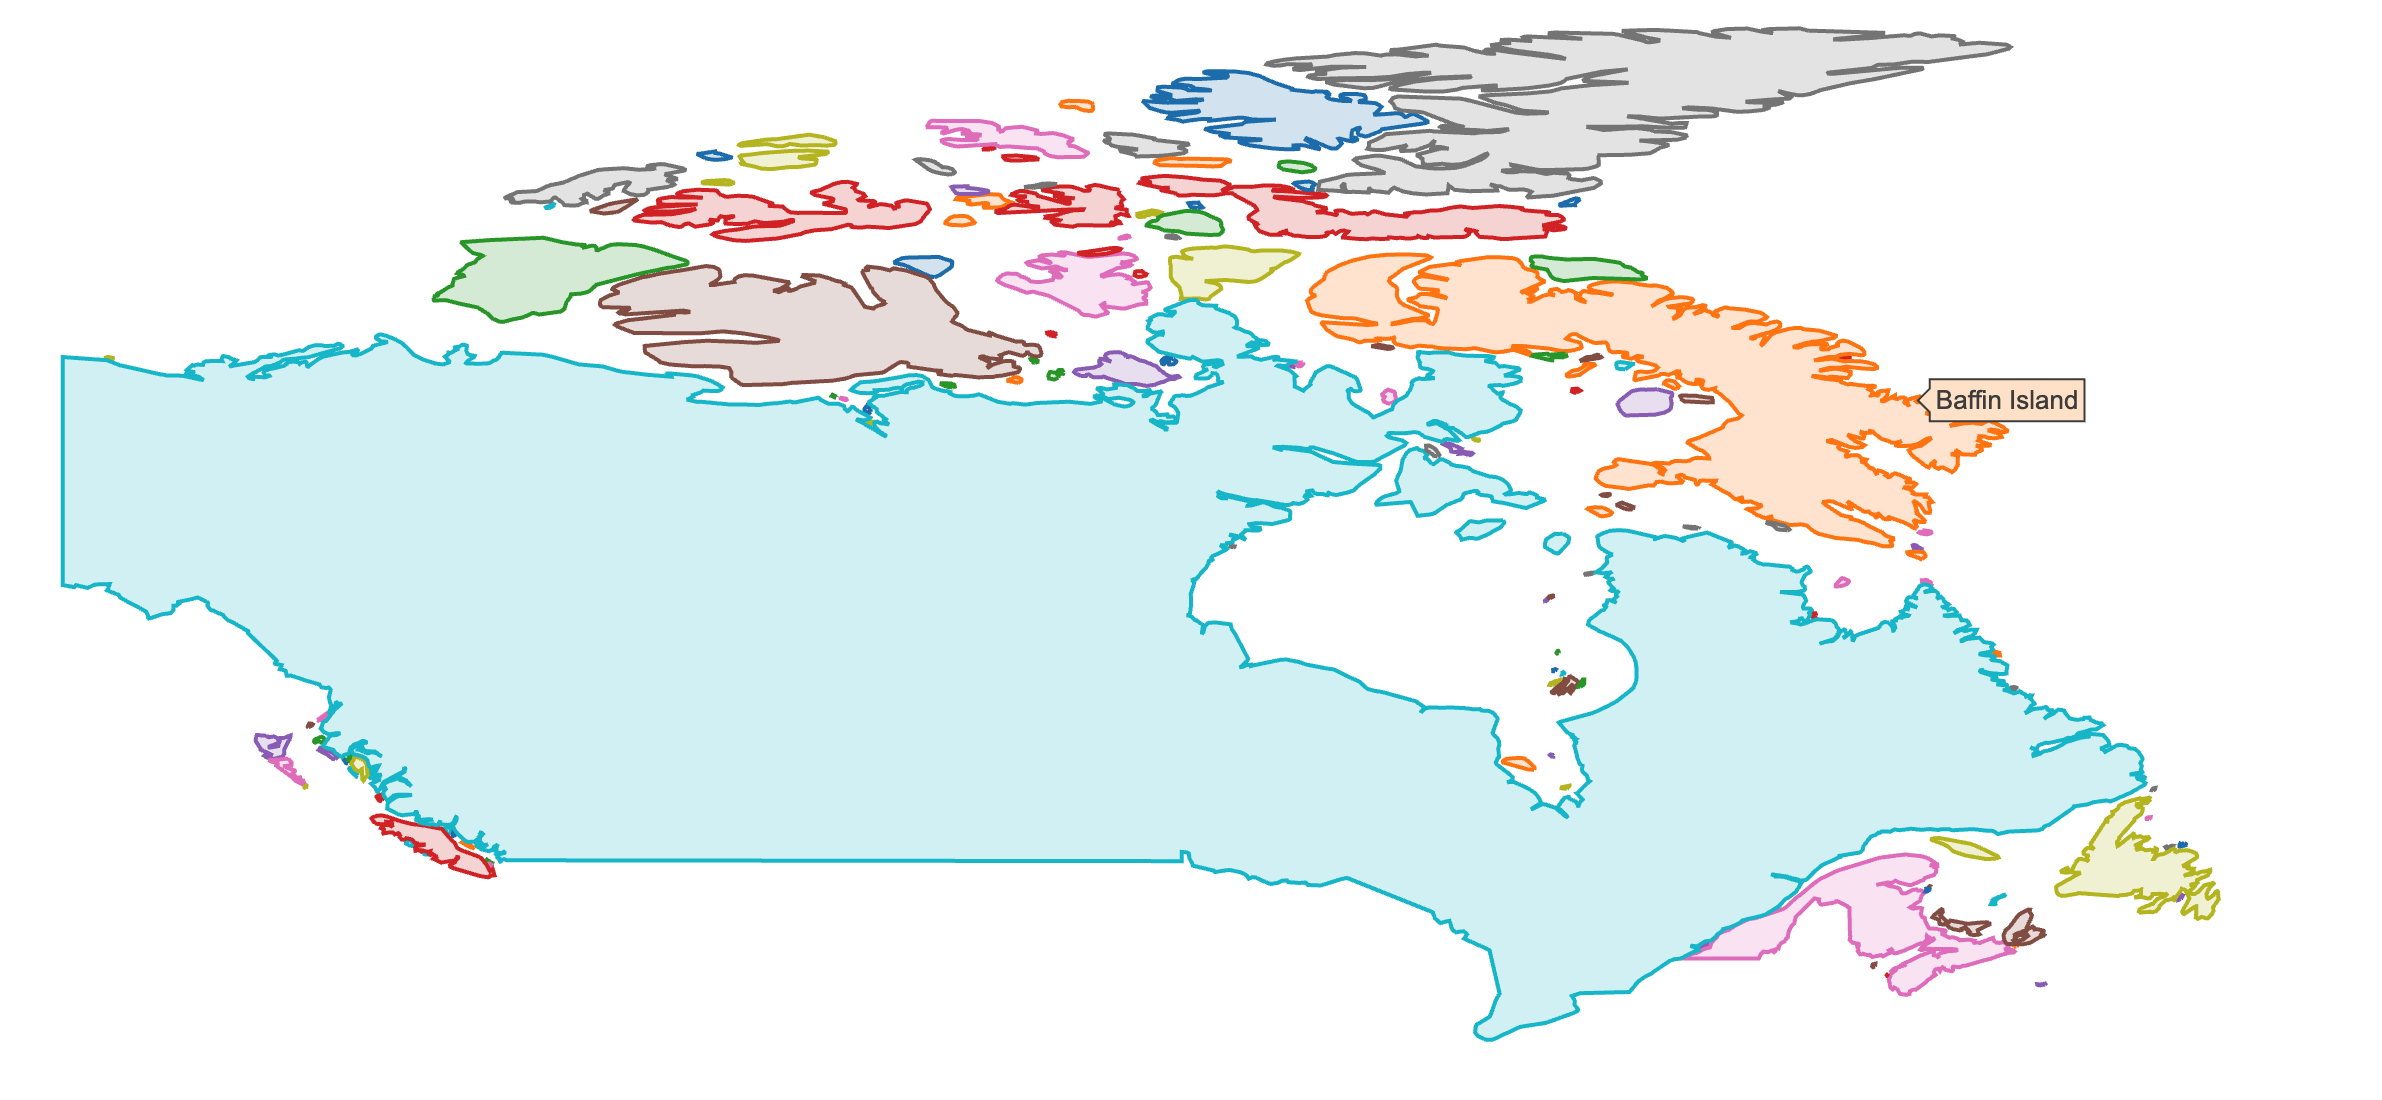
\includegraphics[width=\textwidth]{images/map-canada-split} 

}

\caption{Using \texttt{split} to render polygons with different fills and interactive properties.}\label{fig:map-canada-split}
\end{figure}

\hypertarget{ribbons}{%
\subsection{Ribbons}\label{ribbons}}

\index{add\_trace()@\texttt{add\_trace()}!add\_ribbons()@\texttt{add\_ribbons()}}

Ribbons are useful for showing uncertainty bounds as a function of x. The \texttt{add\_ribbons()} function creates ribbons and requires the arguments: \texttt{x}, \texttt{ymin}, and \texttt{ymax}. The \texttt{augment()} function from the \textbf{broom} package appends observational-level model components (e.g., fitted values stored as a new column \texttt{.fitted}) which is useful for extracting those components in a convenient form for visualization. Figure \ref{fig:broom-lm} shows the fitted values and uncertainty bounds from a linear model object.

\begin{Shaded}
\begin{Highlighting}[]
\NormalTok{m <-}\StringTok{ }\KeywordTok{lm}\NormalTok{(mpg }\OperatorTok{~}\StringTok{ }\NormalTok{wt, }\DataTypeTok{data =}\NormalTok{ mtcars)}
\NormalTok{broom}\OperatorTok{::}\KeywordTok{augment}\NormalTok{(m) }\OperatorTok
\StringTok{  }\KeywordTok{plot_ly}\NormalTok{(}\DataTypeTok{x =} \OperatorTok{~}\NormalTok{wt, }\DataTypeTok{showlegend =} \OtherTok{FALSE}\NormalTok{) }\OperatorTok
\StringTok{  }\KeywordTok{add_markers}\NormalTok{(}\DataTypeTok{y =} \OperatorTok{~}\NormalTok{mpg, }\DataTypeTok{color =} \KeywordTok{I}\NormalTok{(}\StringTok{"black"}\NormalTok{)) }\OperatorTok
\StringTok{  }\KeywordTok{add_ribbons}\NormalTok{(}\DataTypeTok{ymin =} \OperatorTok{~}\NormalTok{.fitted }\OperatorTok{-}\StringTok{ }\FloatTok{1.96} \OperatorTok{*}\StringTok{ }\NormalTok{.se.fit, }
              \DataTypeTok{ymax =} \OperatorTok{~}\NormalTok{.fitted }\OperatorTok{+}\StringTok{ }\FloatTok{1.96} \OperatorTok{*}\StringTok{ }\NormalTok{.se.fit, }
              \DataTypeTok{color =} \KeywordTok{I}\NormalTok{(}\StringTok{"gray80"}\NormalTok{)) }\OperatorTok
\StringTok{  }\KeywordTok{add_lines}\NormalTok{(}\DataTypeTok{y =} \OperatorTok{~}\NormalTok{.fitted, }\DataTypeTok{color =} \KeywordTok{I}\NormalTok{(}\StringTok{"steelblue"}\NormalTok{))}
\end{Highlighting}
\end{Shaded}

\begin{figure}

{\centering 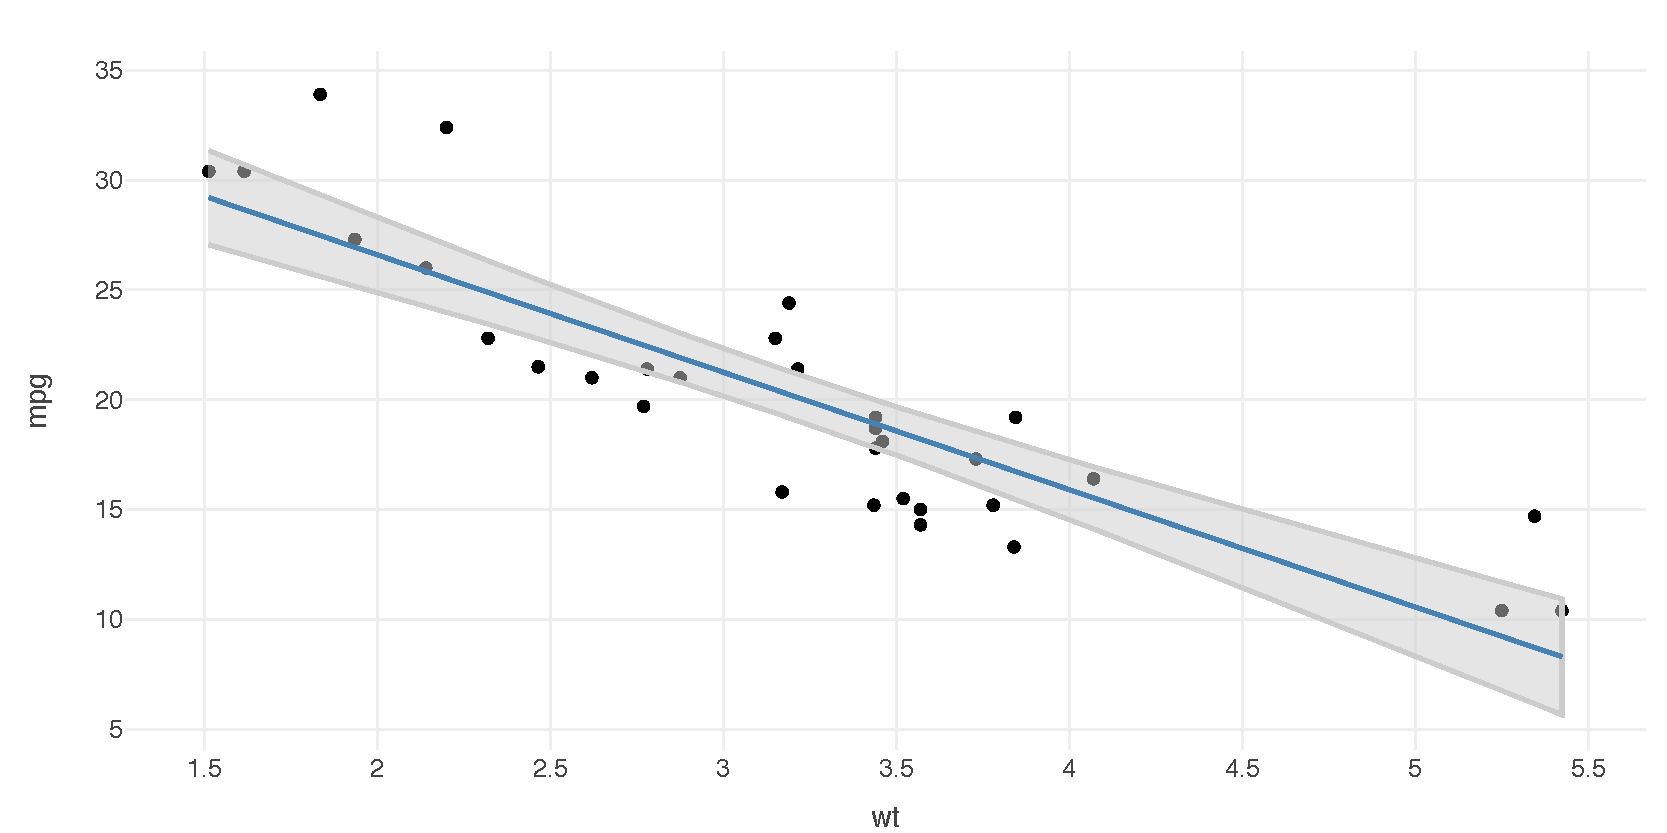
\includegraphics[width=\textwidth]{images/broom-lm} 

}

\caption{Plotting fitted values and uncertainty bounds of a linear model via the \textbf{broom} package.}\label{fig:broom-lm}
\end{figure}

\hypertarget{maps}{%
\chapter{Maps}\label{maps}}

There are numerous ways to make a map with \textbf{plotly} -- each with it's own strengths and weaknesses. Generally speaking the approaches fall under two categories: integrated or custom. Integrated maps leverage plotly.js' built-in support for rendering a basemap layer. Currently there are two supported ways of making integrated maps: either via \href{https://www.mapbox.com/}{Mapbox} or via an integrated d3.js powered basemap. The integrated approach is convenient if you need a quick map and don't necessarily need sophisticated representations of geo-spatial objects. On the other hand, the custom mapping approach offers complete control since you're providing all the information necessary to render the geo-spatial object(s). Section \ref{maps-custom} covers making sophisticated maps (e.g., cartograms) using the \textbf{sf} R package, but it's also possible to make custom \textbf{plotly} maps via other tools for geo-computing (e.g., \textbf{sp}, \textbf{ggmap}, etc).

It's worth noting that \textbf{plotly} aims to be a general purpose visualization library, and thus, doesn't aim to be the most fully featured geo-spatial visualization toolkit. That said, there are benefits to using \textbf{plotly}-based maps since the mapping APIs are very similar to the rest of plotly, and you can leverage larger \textbf{plotly} ecosystem (e.g., linking views client side like Figure \ref{fig:mapbox-bars}). However, if you run into limitations with \textbf{plotly}'s mapping functionality, there is a very rich set of tools for \href{https://geocompr.robinlovelace.net/adv-map.html\#interactive-maps}{interactive geospatial visualization in R}, including but not limited to: \textbf{leaflet}, \textbf{mapview}, \textbf{mapedit}, \textbf{tmap}, and \textbf{mapdeck} \citep{geocomputation}.

\hypertarget{maps-integrated}{%
\section{Integrated maps}\label{maps-integrated}}

\hypertarget{overview-1}{%
\subsection{Overview}\label{overview-1}}

\index{plot\_mapbox()@\texttt{plot\_mapbox()}}

If you have fairly simple latitude/longitude data and want to make a quick map, you may want to try one of \textbf{plotly}'s integrated mapping options (i.e., \texttt{plot\_mapbox()} and \texttt{plot\_geo()}). Generally speaking, you can treat these constructor functions as a drop-in replacement for \texttt{plot\_ly()} and get a dynamic basemap rendered behind your data. Furthermore, all the scatter-based layers we learned about in Section \ref{scatter-traces} work as you'd expect it to with \texttt{plot\_ly()}.\footnote{Unfortunately, non-scatter traces currently don't work with \texttt{plot\_mapbox()}/ \texttt{plot\_geo()} meaning that, for one, raster (i.e., heatmap) maps are not natively supported.} For example, Figure \ref{fig:mapbox-bubble} uses \texttt{plot\_mapbox()} and \texttt{add\_markers()} to create a bubble chart:

\begin{Shaded}
\begin{Highlighting}[]
\KeywordTok{plot_mapbox}\NormalTok{(maps}\OperatorTok{::}\NormalTok{canada.cities) }\OperatorTok
\StringTok{  }\KeywordTok{add_markers}\NormalTok{(}
    \DataTypeTok{x =} \OperatorTok{~}\NormalTok{long, }
    \DataTypeTok{y =} \OperatorTok{~}\NormalTok{lat, }
    \DataTypeTok{size =} \OperatorTok{~}\NormalTok{pop, }
    \DataTypeTok{color =} \OperatorTok{~}\NormalTok{country.etc,}
    \DataTypeTok{colors =} \StringTok{"Accent"}\NormalTok{,}
    \DataTypeTok{text =} \OperatorTok{~}\KeywordTok{paste}\NormalTok{(name, pop),}
    \DataTypeTok{hoverinfo =} \StringTok{"text"}
\NormalTok{  )}
\end{Highlighting}
\end{Shaded}

\begin{figure}

{\centering 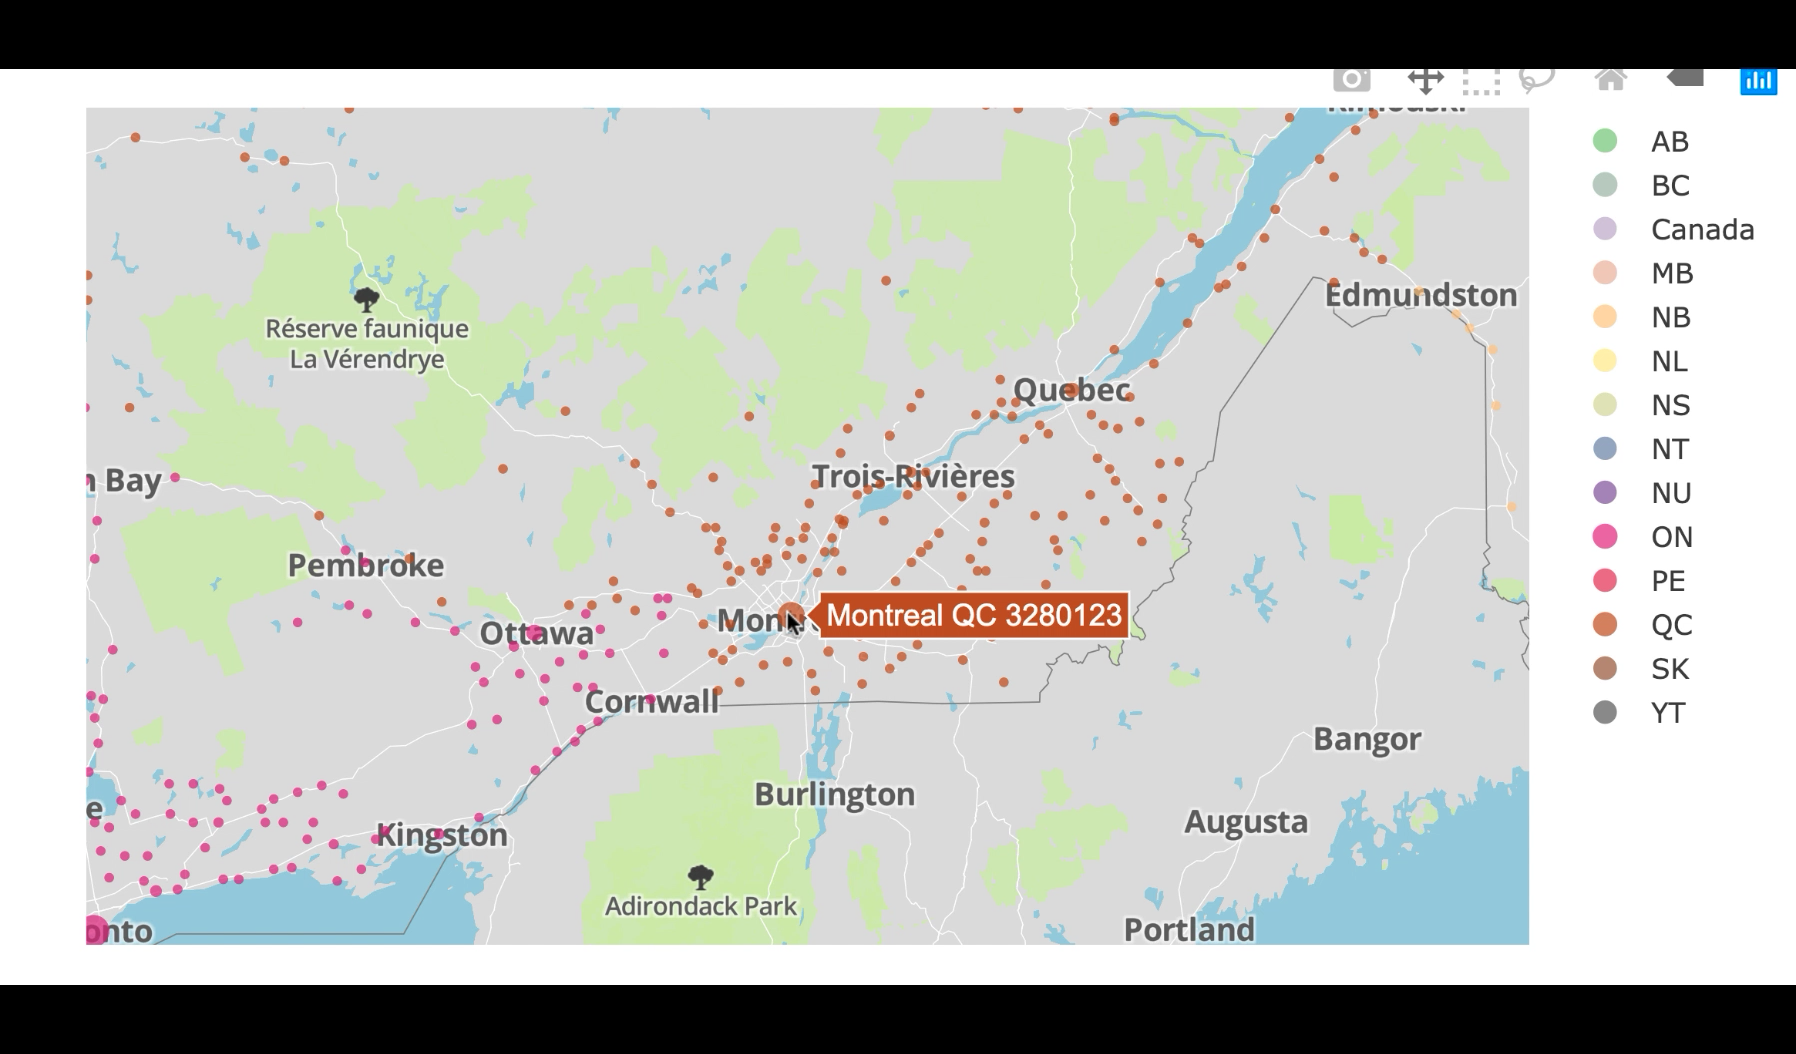
\includegraphics[width=\textwidth]{vimeo-images/317352934/final} 

}

\caption{A mapbox powered bubble chart showing the population of various cities in Canada. For a video demonstration of the interactive, see \url{https://bit.ly/mapbox-bubble}. For the interactive, see \url{https://plotly-r.com/interactives/mapbox-bubble.html}}\label{fig:mapbox-bubble}
\end{figure}

\index{plot\_mapbox()@\texttt{plot\_mapbox()}!Basemap style}

The Mapbox basemap styling is controlled through the \href{https://plot.ly/r/reference/\#layout-mapbox-style}{\texttt{layout.mapbox.style}} attribute. The \textbf{plotly} package comes with support for 7 different styles, but you can also supply a custom URL to a \href{https://docs.mapbox.com/help/tutorials/create-a-custom-style/}{custom mapbox style}. To obtain all the pre-packaged basemap style names, you can grab them from the official plotly.js \texttt{schema()}:

\begin{Shaded}
\begin{Highlighting}[]
\NormalTok{styles <-}\StringTok{ }\KeywordTok{schema}\NormalTok{()}\OperatorTok{$}\NormalTok{layout}\OperatorTok{$}\NormalTok{layoutAttributes}\OperatorTok{$}\NormalTok{mapbox}\OperatorTok{$}\NormalTok{style}\OperatorTok{$}\NormalTok{values}
\NormalTok{styles}
\CommentTok{#> [1] "basic"             "streets"          }
\CommentTok{#> [3] "outdoors"          "light"            }
\CommentTok{#> [5] "dark"              "satellite"        }
\CommentTok{#> [7] "satellite-streets"}
\end{Highlighting}
\end{Shaded}

Any one of these values can be used for a mapbox style. Figure \ref{fig:satellite} demonstrates the satellite earth imagery basemap.

\begin{Shaded}
\begin{Highlighting}[]
\KeywordTok{layout}\NormalTok{(}
  \KeywordTok{plot_mapbox}\NormalTok{(), }
  \DataTypeTok{mapbox =} \KeywordTok{list}\NormalTok{(}\DataTypeTok{style =} \StringTok{"satellite"}\NormalTok{)}
\NormalTok{)}
\end{Highlighting}
\end{Shaded}

\begin{figure}

{\centering \includegraphics[width=\textwidth]{vimeo-images/326683897/final} 

}

\caption{Zooming in on earth satellite imagery using \texttt{plot\_mapbox()}. For a video demonstration of the interactive, see \url{https://bit.ly/mapbox-satellite}. For the interactive, see \url{https://plotly-r.com/interactives/satellite.html}}\label{fig:satellite}
\end{figure}

Figure \ref{fig:mapbox-style-dropdown} demonstrates how to create an integrated plotly.js dropdown menu to control the basemap style via the \href{https://plot.ly/r/reference/\#layout-updatemenus-items-updatemenu-buttons}{\texttt{layout.updatemenus}} attribute. The idea behind an integrated plotly.js dropdown is to supply a list of buttons (i.e., menu items) where each button invokes a plotly.js method with some arguments. In this case, each button uses the \href{https://plot.ly/javascript/plotlyjs-function-reference/}{relayout} method to modify the \texttt{layout.mapbox.style} attribute.\footnote{To see more examples of creating and using plotly.js' integrated dropdown functionality to modify graphs, see \url{https://plot.ly/r/dropdowns/}}

\index{layout()@\texttt{layout()}!updatemenus@\texttt{updatemenus}}

\begin{Shaded}
\begin{Highlighting}[]
\NormalTok{style_buttons <-}\StringTok{ }\KeywordTok{lapply}\NormalTok{(styles, }\ControlFlowTok{function}\NormalTok{(s) \{}
  \KeywordTok{list}\NormalTok{(}
    \DataTypeTok{label =}\NormalTok{ s, }
    \DataTypeTok{method =} \StringTok{"relayout"}\NormalTok{, }
    \DataTypeTok{args =} \KeywordTok{list}\NormalTok{(}\StringTok{"mapbox.style"}\NormalTok{, s)}
\NormalTok{  )}
\NormalTok{\})}
\KeywordTok{layout}\NormalTok{(}
  \KeywordTok{plot_mapbox}\NormalTok{(), }
  \DataTypeTok{mapbox =} \KeywordTok{list}\NormalTok{(}\DataTypeTok{style =} \StringTok{"dark"}\NormalTok{),}
  \DataTypeTok{updatemenus =} \KeywordTok{list}\NormalTok{(}
    \KeywordTok{list}\NormalTok{(}\DataTypeTok{y =} \FloatTok{0.8}\NormalTok{, }\DataTypeTok{buttons =}\NormalTok{ style_buttons)}
\NormalTok{  )}
\NormalTok{)}
\end{Highlighting}
\end{Shaded}

\begin{figure}

{\centering \includegraphics[width=\textwidth]{vimeo-images/326684625/final} 

}

\caption{Providing a dropdown menu to control the styling of the mapbox baselayer. For a video demonstration of the interactive, see \url{https://bit.ly/mapbox-style-dropdown}. For the interactive, see \url{https://plotly-r.com/interactives/mapbox-style-dropdown.html}}\label{fig:mapbox-style-dropdown}
\end{figure}

\index{plot\_geo()@\texttt{plot\_geo()}}

The other integrated mapping solution in \textbf{plotly} is \texttt{plot\_geo()}. Compared to \texttt{plot\_mapbox()}, this approach has support for different mapping projections, but styling the basemap is limited and can be more cumbersome. Figure \ref{fig:geo-flights} demonstrates using \texttt{plot\_geo()} in conjunction with \texttt{add\_markers()} and \texttt{add\_segments()} to visualize flight paths within the United States. Whereas \texttt{plot\_mapbox()} is fixed to a mercator projection, the \texttt{plot\_geo()} constructor has a handful of different projection available to it, including the orthographic projection which gives the illusion of the 3D globe.

\index{plot\_geo()@\texttt{plot\_geo()}!layout.geo@\texttt{layout(geo = ...)}}

\begin{Shaded}
\begin{Highlighting}[]
\KeywordTok{library}\NormalTok{(plotly)}
\KeywordTok{library}\NormalTok{(dplyr)}
\CommentTok{# airport locations}
\NormalTok{air <-}\StringTok{ }\KeywordTok{read.csv}\NormalTok{(}
  \StringTok{'https://plotly-r.com/data-raw/airport_locations.csv'}
\NormalTok{)}
\CommentTok{# flights between airports}
\NormalTok{flights <-}\StringTok{ }\KeywordTok{read.csv}\NormalTok{(}
  \StringTok{'https://plotly-r.com/data-raw/flight_paths.csv'}
\NormalTok{)}
\NormalTok{flights}\OperatorTok{$}\NormalTok{id <-}\StringTok{ }\KeywordTok{seq_len}\NormalTok{(}\KeywordTok{nrow}\NormalTok{(flights))}

\CommentTok{# map projection}
\NormalTok{geo <-}\StringTok{ }\KeywordTok{list}\NormalTok{(}
  \DataTypeTok{projection =} \KeywordTok{list}\NormalTok{(}
    \DataTypeTok{type =} \StringTok{'orthographic'}\NormalTok{,}
    \DataTypeTok{rotation =} \KeywordTok{list}\NormalTok{(}\DataTypeTok{lon =} \DecValTok{-100}\NormalTok{, }\DataTypeTok{lat =} \DecValTok{40}\NormalTok{, }\DataTypeTok{roll =} \DecValTok{0}\NormalTok{)}
\NormalTok{  ),}
  \DataTypeTok{showland =} \OtherTok{TRUE}\NormalTok{,}
  \DataTypeTok{landcolor =} \KeywordTok{toRGB}\NormalTok{(}\StringTok{"gray95"}\NormalTok{),}
  \DataTypeTok{countrycolor =} \KeywordTok{toRGB}\NormalTok{(}\StringTok{"gray80"}\NormalTok{)}
\NormalTok{)}

\KeywordTok{plot_geo}\NormalTok{(}\DataTypeTok{color =} \KeywordTok{I}\NormalTok{(}\StringTok{"red"}\NormalTok{)) }\OperatorTok
\StringTok{  }\KeywordTok{add_markers}\NormalTok{(}
    \DataTypeTok{data =}\NormalTok{ air, }\DataTypeTok{x =} \OperatorTok{~}\NormalTok{long, }\DataTypeTok{y =} \OperatorTok{~}\NormalTok{lat, }\DataTypeTok{text =} \OperatorTok{~}\NormalTok{airport,}
    \DataTypeTok{size =} \OperatorTok{~}\NormalTok{cnt, }\DataTypeTok{hoverinfo =} \StringTok{"text"}\NormalTok{, }\DataTypeTok{alpha =} \FloatTok{0.5}
\NormalTok{  ) }\OperatorTok
\StringTok{  }\KeywordTok{add_segments}\NormalTok{(}
    \DataTypeTok{data =} \KeywordTok{group_by}\NormalTok{(flights, id),}
    \DataTypeTok{x =} \OperatorTok{~}\NormalTok{start_lon, }\DataTypeTok{xend =} \OperatorTok{~}\NormalTok{end_lon,}
    \DataTypeTok{y =} \OperatorTok{~}\NormalTok{start_lat, }\DataTypeTok{yend =} \OperatorTok{~}\NormalTok{end_lat,}
    \DataTypeTok{alpha =} \FloatTok{0.3}\NormalTok{, }\DataTypeTok{size =} \KeywordTok{I}\NormalTok{(}\DecValTok{1}\NormalTok{), }\DataTypeTok{hoverinfo =} \StringTok{"none"}
\NormalTok{  ) }\OperatorTok
\StringTok{  }\KeywordTok{layout}\NormalTok{(}\DataTypeTok{geo =}\NormalTok{ geo, }\DataTypeTok{showlegend =} \OtherTok{FALSE}\NormalTok{)}
\end{Highlighting}
\end{Shaded}

\begin{figure}

{\centering \includegraphics[width=\textwidth]{vimeo-images/317358033/final} 

}

\caption{Using the integrated orthographic projection to visualize flight patterns on a `3D' globe. For a video demonstration of the interactive, see \url{https://bit.ly/geo-flights}. For the interactive, see \url{https://plotly-r.com/interactives/geo-flights.html}}\label{fig:geo-flights}
\end{figure}

One nice thing about \texttt{plot\_geo()} is that it automatically projects geometries into the proper coordinate system defined by the map projection. For example, in Figure \ref{fig:maps} the simple line segment is straight when using \texttt{plot\_mapbox()} yet curved when using \texttt{plot\_geo()}. It's possible to achieve the same effect using \texttt{plot\_ly()} or \texttt{plot\_mapbox()}, but the relevant marker/line/polygon data has to be put into an \textbf{sf} data structure before rendering (see Section \ref{sf} for more details).

\index{add\_trace()@\texttt{add\_trace()}!add\_segments()@\texttt{add\_segments()}}
\indexc{htmltools::tagList()}

\begin{Shaded}
\begin{Highlighting}[]
\NormalTok{map1 <-}\StringTok{ }\KeywordTok{plot_mapbox}\NormalTok{() }\OperatorTok\StringTok{ }
\StringTok{  }\KeywordTok{add_segments}\NormalTok{(}\DataTypeTok{x =} \DecValTok{-100}\NormalTok{, }\DataTypeTok{xend =} \DecValTok{-50}\NormalTok{, }\DataTypeTok{y =} \DecValTok{50}\NormalTok{, }\DataTypeTok{yend =} \DecValTok{75}\NormalTok{) }\OperatorTok
\StringTok{  }\KeywordTok{layout}\NormalTok{(}
    \DataTypeTok{mapbox =} \KeywordTok{list}\NormalTok{(}
      \DataTypeTok{zoom =} \DecValTok{0}\NormalTok{,}
      \DataTypeTok{center =} \KeywordTok{list}\NormalTok{(}\DataTypeTok{lat =} \DecValTok{65}\NormalTok{, }\DataTypeTok{lon =} \DecValTok{-75}\NormalTok{)}
\NormalTok{    )}
\NormalTok{  )}

\NormalTok{map2 <-}\StringTok{ }\KeywordTok{plot_geo}\NormalTok{() }\OperatorTok\StringTok{ }
\StringTok{  }\KeywordTok{add_segments}\NormalTok{(}\DataTypeTok{x =} \DecValTok{-100}\NormalTok{, }\DataTypeTok{xend =} \DecValTok{-50}\NormalTok{, }\DataTypeTok{y =} \DecValTok{50}\NormalTok{, }\DataTypeTok{yend =} \DecValTok{75}\NormalTok{) }\OperatorTok
\StringTok{  }\KeywordTok{layout}\NormalTok{(}\DataTypeTok{geo =} \KeywordTok{list}\NormalTok{(}\DataTypeTok{projection =} \KeywordTok{list}\NormalTok{(}\DataTypeTok{type =} \StringTok{"mercator"}\NormalTok{)))}

\KeywordTok{library}\NormalTok{(htmltools)}
\KeywordTok{browsable}\NormalTok{(}\KeywordTok{tagList}\NormalTok{(map1, map2))}
\end{Highlighting}
\end{Shaded}

\begin{figure}

{\centering \includegraphics[width=\textwidth]{images/maps} 

}

\caption{A comparison of \textbf{plotly}'s integrated mapping solutions: \texttt{plot\_mapbox()} (top) and \texttt{plot\_geo()} (bottom). The \texttt{plot\_geo()} approach will transform line segments to correctly reflect their projection into a non-cartesian coordinate system.}\label{fig:maps}
\end{figure}

\hypertarget{choropleths}{%
\subsection{Choropleths}\label{choropleths}}

\index{Chart types!Choropleth}

In addition to scatter traces, both of the integrated mapping solutions (i.e., \texttt{plot\_mapbox()} and \texttt{plot\_geo()}) have an optimized choropleth trace type (i.e., the \href{https://plot.ly/r/reference/\#choroplethmapbox}{choroplethmapbox} and \href{https://plot.ly/r/reference/\#choropleth}{choropleth} trace types). Comparatively speaking, choroplethmapbox is more powerful because you can fully specify the feature collection using GeoJSON, but the choropleth trace can be a bit easier to use if it fits your use case.

Figure \ref{fig:us-density} shows the population density of the U.S. via the choropleth trace using the U.S. state data from the \textbf{datasets} package \citep{RCore}. By simply providing a \href{https://plot.ly/r/reference/\#choropleth-z}{\texttt{z}} attribute, \texttt{plotly\_geo()} objects will try to create a choropleth, but you'll also need to provide \href{https://plot.ly/r/reference/\#choropleth-locations}{\texttt{locations}} and a \href{https://plot.ly/r/reference/\#choropleth-locationmode}{\texttt{locationmode}}. It's worth noting that the \texttt{locationmode} is currently limited to countries and US states, so if you need to a different geo-unit (e.g., counties, municipalities, etc), you should use the choroplethmapbox trace type and/or use a ``custom'' mapping approach as discussed in Section \ref{maps-custom}.

\index{plot\_geo()@\texttt{plot\_geo()}!Choropleth}

\begin{Shaded}
\begin{Highlighting}[]
\NormalTok{density <-}\StringTok{ }\NormalTok{state.x77[, }\StringTok{"Population"}\NormalTok{] }\OperatorTok{/}\StringTok{ }\NormalTok{state.x77[, }\StringTok{"Area"}\NormalTok{]}

\NormalTok{g <-}\StringTok{ }\KeywordTok{list}\NormalTok{(}
  \DataTypeTok{scope =} \StringTok{'usa'}\NormalTok{,}
  \DataTypeTok{projection =} \KeywordTok{list}\NormalTok{(}\DataTypeTok{type =} \StringTok{'albers usa'}\NormalTok{),}
  \DataTypeTok{lakecolor =} \KeywordTok{toRGB}\NormalTok{(}\StringTok{'white'}\NormalTok{)}
\NormalTok{)}

\KeywordTok{plot_geo}\NormalTok{() }\OperatorTok
\StringTok{  }\KeywordTok{add_trace}\NormalTok{(}
    \DataTypeTok{z =} \OperatorTok{~}\NormalTok{density, }\DataTypeTok{text =}\NormalTok{ state.name, }\DataTypeTok{span =} \KeywordTok{I}\NormalTok{(}\DecValTok{0}\NormalTok{),}
    \DataTypeTok{locations =}\NormalTok{ state.abb, }\DataTypeTok{locationmode =} \StringTok{'USA-states'}
\NormalTok{  ) }\OperatorTok
\StringTok{  }\KeywordTok{layout}\NormalTok{(}\DataTypeTok{geo =}\NormalTok{ g)}
\end{Highlighting}
\end{Shaded}

\begin{figure}

{\centering \includegraphics[width=\textwidth]{images/us-density} 

}

\caption{A map of U.S. population density using the \texttt{state.x77} data from the \textbf{datasets} package.}\label{fig:us-density}
\end{figure}

Choroplethmapbox is more flexible than choropleth because you supply your own GeoJSON definition of the choropleth via the \texttt{geojson} attribute. Currently this attribute must be a URL pointing to a geojson file. Moreover, the \texttt{location} should point to a top-level id attribute of each feature within the geojson file. Figure \ref{fig:us-density-geojson} demonstrates how we could visualize the same information as Figure \ref{fig:us-density}, but this time using choroplethmapbox.

\index{plot\_mapbox()@\texttt{plot\_mapbox()}!Choropleth}

\begin{Shaded}
\begin{Highlighting}[]
\KeywordTok{plot_ly}\NormalTok{() }\OperatorTok
\StringTok{  }\KeywordTok{add_trace}\NormalTok{(}
    \DataTypeTok{type =} \StringTok{"choroplethmapbox"}\NormalTok{,}
    \CommentTok{# See how this GeoJSON URL was generated at}
    \CommentTok{# https://plotly-r.com/data-raw/us-states.R}
    \DataTypeTok{geojson =} \KeywordTok{paste}\NormalTok{(}\KeywordTok{c}\NormalTok{(}
      \StringTok{"https://gist.githubusercontent.com/cpsievert/"}\NormalTok{,}
      \StringTok{"7cdcb444fb2670bd2767d349379ae886/raw/"}\NormalTok{,}
      \StringTok{"cf5631bfd2e385891bb0a9788a179d7f023bf6c8/"}\NormalTok{, }
      \StringTok{"us-states.json"}
\NormalTok{    ), }\DataTypeTok{collapse =} \StringTok{""}\NormalTok{),}
    \DataTypeTok{locations =} \KeywordTok{row.names}\NormalTok{(state.x77),}
    \DataTypeTok{z =}\NormalTok{ state.x77[, }\StringTok{"Population"}\NormalTok{] }\OperatorTok{/}\StringTok{ }\NormalTok{state.x77[, }\StringTok{"Area"}\NormalTok{],}
    \DataTypeTok{span =} \KeywordTok{I}\NormalTok{(}\DecValTok{0}\NormalTok{)}
\NormalTok{  ) }\OperatorTok
\StringTok{  }\KeywordTok{layout}\NormalTok{(}
    \DataTypeTok{mapbox =} \KeywordTok{list}\NormalTok{(}
      \DataTypeTok{style =} \StringTok{"light"}\NormalTok{,}
      \DataTypeTok{zoom =} \DecValTok{4}\NormalTok{,}
      \DataTypeTok{center =} \KeywordTok{list}\NormalTok{(}\DataTypeTok{lon =} \FloatTok{-98.58}\NormalTok{, }\DataTypeTok{lat =} \FloatTok{39.82}\NormalTok{)}
\NormalTok{    )}
\NormalTok{  ) }\OperatorTok
\StringTok{  }\KeywordTok{config}\NormalTok{(}
    \DataTypeTok{mapboxAccessToken =} \KeywordTok{Sys.getenv}\NormalTok{(}\StringTok{"MAPBOX_TOKEN"}\NormalTok{),}
    \CommentTok{# Workaround to make sure image download uses full container}
    \CommentTok{# size https://github.com/plotly/plotly.js/pull/3746}
    \DataTypeTok{toImageButtonOptions =} \KeywordTok{list}\NormalTok{(}
      \DataTypeTok{format =} \StringTok{"svg"}\NormalTok{, }
      \DataTypeTok{width =} \OtherTok{NULL}\NormalTok{, }
      \DataTypeTok{height =} \OtherTok{NULL}
\NormalTok{    )}
\NormalTok{  )}
\end{Highlighting}
\end{Shaded}

\begin{figure}

{\centering \includegraphics[width=\textwidth]{images/us-density-geojson} 

}

\caption{Another map of U.S. population density, this time using choroplethmapbox with a custom GeoJSON file.}\label{fig:us-density-geojson}
\end{figure}

Figures \ref{fig:us-density} and \ref{fig:us-density-geojson} aren't an ideal way to visualize state population a graphical perception point of view. We typically use the color in choropleths to encode a numeric variable (e.g., GDP, net exports, average SAT score, etc) and the eye naturally perceives the area that a particular color covers as proportional to its overall effect. This ends up being misleading since the area the color covers typically has no sensible relationship with the data encoded by the color. A classic example of this misleading effect in action is in US election maps -- the proportion of red to blue coloring is not representative of the overall popular vote \citep{election-maps}.

Cartograms are an approach to reducing this misleading effect and grants another dimension to encode data through the size of geo-spatial features. Section \ref{cartograms} covers how to render cartograms in \textbf{plotly} using \textbf{sf} and \textbf{cartogram}.

\hypertarget{maps-custom}{%
\section{Custom maps}\label{maps-custom}}

\hypertarget{sf}{%
\subsection{Simple features (sf)}\label{sf}}

The \textbf{sf} R package is a modern approach to working with geo-spatial data structures based on tidy data principles \citep{sf, tidy-data}. The key idea behind \textbf{sf} is that it stores geo-spatial geometries in a \href{https://jennybc.github.io/purrr-tutorial/ls13_list-columns.html}{list-column} of a data frame. This allows each row to represent the real unit of observation/interest -- whether it's a polygon, multi-polygon, point, line, or even a collection of these features -- and as a result, works seamlessly inside larger tidy workflows.\footnote{This is way more intuitive compared to older workflows based on, say using \texttt{ggplot2::fortify()} to obtain a data structure where a row to represents particular point along a feature and having another column track which point belongs to each feature (\href{https://gis.stackexchange.com/questions/165974/r-fortify-causing-polygons-to-tear}{for example}).} The \textbf{sf} package itself does not really provide geo-spatial data -- it provides the framework and utilities for storing and computing on geo-spatial data structures in an opinionated way.

There are numerous packages for accessing geo-spatial data as simple features data structures. A couple notable examples include \textbf{rnaturalearth} and \textbf{USAboundaries}. The \textbf{rnaturalearth} package is better for obtaining any map data in the world via an API provided by \url{https://www.naturalearthdata.com/} \citep{rnaturalearth}. The \textbf{USAboundaries} package is great for obtaining map data for the United States at any point in history \citep{USAboundaries}. It doesn't really matter what tool you use to obtain or create an \textbf{sf} object -- once you have one, \texttt{plot\_ly()} knows how to render it:

\begin{Shaded}
\begin{Highlighting}[]
\KeywordTok{library}\NormalTok{(rnaturalearth)}
\NormalTok{world <-}\StringTok{ }\KeywordTok{ne_countries}\NormalTok{(}\DataTypeTok{returnclass =} \StringTok{"sf"}\NormalTok{)}
\KeywordTok{class}\NormalTok{(world)}
\CommentTok{#> [1] "sf"    "data.frame"}
\KeywordTok{plot_ly}\NormalTok{(world, }\DataTypeTok{color =} \KeywordTok{I}\NormalTok{(}\StringTok{"gray90"}\NormalTok{), }\DataTypeTok{stroke =} \KeywordTok{I}\NormalTok{(}\StringTok{"black"}\NormalTok{), }\DataTypeTok{span =} \KeywordTok{I}\NormalTok{(}\DecValTok{1}\NormalTok{))}
\end{Highlighting}
\end{Shaded}

\begin{figure}

{\centering \includegraphics[width=\textwidth]{images/world} 

}

\caption{Rendering all the world's countries using \texttt{plot\_ly()} and the \texttt{ne\_countries()} function from the \textbf{rnaturalearth} package.}\label{fig:world}
\end{figure}

How does \texttt{plot\_ly()} know how to render the countries? It's because the geo-spatial features are encoded in special (geometry) list-column. Also, meta-data about the geo-spatial structure are retained as special attributes of the data. Figure \ref{fig:view-sf} augments the print method for \textbf{sf} to data frames to demonstrate that all the information needed to render the countries (i.e., polygons) in Figure \ref{fig:world} is contained within the \texttt{world} data frame. Note also, that \textbf{sf} provides special \textbf{dplyr} methods for this special class of data frame so that you can treat data manipulations as if it were a `tidy' data structure. One thing about this method is that the special `geometry' column is always retained -- if we try to just select the \texttt{name} column, then we get both the name and the geometry.

\begin{Shaded}
\begin{Highlighting}[]
\KeywordTok{library}\NormalTok{(sf)}
\NormalTok{world }\OperatorTok
\StringTok{  }\KeywordTok{select}\NormalTok{(name) }\OperatorTok
\StringTok{  }\KeywordTok{print}\NormalTok{(}\DataTypeTok{n =} \DecValTok{4}\NormalTok{)}
\end{Highlighting}
\end{Shaded}

\begin{figure}

{\centering \includegraphics[width=\textwidth]{images/view-sf} 

}

\caption{A diagram of a simple features data frame. The geometry column tracks the spatial features attached to each row in the data frame.}\label{fig:view-sf}
\end{figure}

There are actually 4 different ways to render \textbf{sf} objects with \textbf{plotly}: \texttt{plot\_ly()}, \texttt{plot\_mapbox()}, \texttt{plot\_geo()}, and via \textbf{ggplot2}'s \texttt{geom\_sf()}. These functions render multiple polygons using a \emph{single} trace by default, which is fast, but you may want to leverage the added flexibility of multiple traces. For example, a given trace can only have one \texttt{fillcolor}, so it's impossible to render multiple polygons with different colors using a single trace. For this reason, if you want to vary the color of multiple polygons, make sure the \texttt{split} by a unique identifier (e.g.~\texttt{name}), as done in Figure \ref{fig:split-color}. Note that, as discussed for line charts in Figure \ref{fig:scatter-lines}, using multiple traces automatically adds the ability to filter \texttt{name} via legend entries.

\begin{Shaded}
\begin{Highlighting}[]
\NormalTok{canada <-}\StringTok{ }\KeywordTok{ne_states}\NormalTok{(}\DataTypeTok{country =} \StringTok{"Canada"}\NormalTok{, }\DataTypeTok{returnclass =} \StringTok{"sf"}\NormalTok{)}
\KeywordTok{plot_ly}\NormalTok{(canada, }\DataTypeTok{split =} \OperatorTok{~}\NormalTok{name, }\DataTypeTok{color =} \OperatorTok{~}\NormalTok{provnum_ne)}
\end{Highlighting}
\end{Shaded}

\begin{figure}

{\centering \includegraphics[width=\textwidth]{images/split-color} 

}

\caption{Using \texttt{split} and \texttt{color} to create a choropleth map of provinces in Canada.}\label{fig:split-color}
\end{figure}

Another important feature for maps that may require you to \texttt{split} multiple polygons into multiple traces is the ability to display a different hover-on-fill for each polygon. By providing \texttt{text} that is unique within each polygon and specifying \texttt{hoveron=\textquotesingle{}fills\textquotesingle{}}, the tooltip behavior is tied to the trace's fill (instead of displayed at each point along the polygon).

\begin{Shaded}
\begin{Highlighting}[]
\KeywordTok{plot_ly}\NormalTok{(}
\NormalTok{  canada, }
  \DataTypeTok{split =} \OperatorTok{~}\NormalTok{name, }
  \DataTypeTok{color =} \KeywordTok{I}\NormalTok{(}\StringTok{"gray90"}\NormalTok{), }
  \DataTypeTok{text =} \OperatorTok{~}\KeywordTok{paste}\NormalTok{(name, }\StringTok{"is }\CharTok{\textbackslash{}n}\StringTok{ province number"}\NormalTok{, provnum_ne),}
  \DataTypeTok{hoveron =} \StringTok{"fills"}\NormalTok{,}
  \DataTypeTok{hoverinfo =} \StringTok{"text"}\NormalTok{,}
  \DataTypeTok{showlegend =} \OtherTok{FALSE}
\NormalTok{)}
\end{Highlighting}
\end{Shaded}

\begin{figure}

{\centering \includegraphics[width=\textwidth]{images/split-text} 

}

\caption{Using \texttt{split}, \texttt{text}, and \texttt{hoveron=\textquotesingle{}fills\textquotesingle{}} to display a tooltip specific to each Canadian province.}\label{fig:split-text}
\end{figure}

Although the integrated mapping approaches (\texttt{plot\_mapbox()} and \texttt{plot\_geo()}) can render \textbf{sf} objects, the custom mapping approaches (\texttt{plot\_ly()} and \texttt{geom\_sf()}) are more flexible because they allow for any well-defined mapping projection. Working with and understanding map projections can be intimidating for a causal map maker. Thankfully, there are nice resources for searching map projections in a human-friendly interface, like \url{http://spatialreference.org/}. Through this website, one can search desirable projections for a given portion of the globe and extract commands for projecting their geo-spatial objects into that projection. One way to perform the projection is to supply the relevant PROJ4 command to the \texttt{st\_transform()} function in \textbf{sf} \citep{PROJ}.

\begin{Shaded}
\begin{Highlighting}[]
\CommentTok{# filter the world sf object down to canada}
\NormalTok{canada <-}\StringTok{ }\KeywordTok{filter}\NormalTok{(world, name }\OperatorTok{==}\StringTok{ "Canada"}\NormalTok{)}
\CommentTok{# coerce cities lat/long data to an official sf object}
\NormalTok{cities <-}\StringTok{ }\KeywordTok{st_as_sf}\NormalTok{(}
\NormalTok{  maps}\OperatorTok{::}\NormalTok{canada.cities, }
  \DataTypeTok{coords =} \KeywordTok{c}\NormalTok{(}\StringTok{"long"}\NormalTok{, }\StringTok{"lat"}\NormalTok{),}
  \DataTypeTok{crs =} \DecValTok{4326}
\NormalTok{)}

\CommentTok{# A PROJ4 projection designed for Canada}
\CommentTok{# http://spatialreference.org/ref/sr-org/7/}
\CommentTok{# http://spatialreference.org/ref/sr-org/7/proj4/}
\NormalTok{moll_proj <-}\StringTok{ "+proj=moll +lon_0=0 +x_0=0 +y_0=0 +ellps=WGS84 }
\StringTok{+units=m +no_defs"}

\CommentTok{# perform the projections}
\NormalTok{canada <-}\StringTok{ }\KeywordTok{st_transform}\NormalTok{(canada, moll_proj)}
\NormalTok{cities <-}\StringTok{ }\KeywordTok{st_transform}\NormalTok{(cities, moll_proj)}

\CommentTok{# plot with geom_sf()}
\NormalTok{p <-}\StringTok{ }\KeywordTok{ggplot}\NormalTok{() }\OperatorTok{+}\StringTok{ }
\StringTok{  }\KeywordTok{geom_sf}\NormalTok{(}\DataTypeTok{data =}\NormalTok{ canada) }\OperatorTok{+}
\StringTok{  }\KeywordTok{geom_sf}\NormalTok{(}\DataTypeTok{data =}\NormalTok{ cities, }\KeywordTok{aes}\NormalTok{(}\DataTypeTok{size =}\NormalTok{ pop), }\DataTypeTok{color =} \StringTok{"red"}\NormalTok{, }\DataTypeTok{alpha =} \FloatTok{0.3}\NormalTok{)}
\KeywordTok{ggplotly}\NormalTok{(p)}
\end{Highlighting}
\end{Shaded}

\begin{figure}

{\centering \includegraphics[width=\textwidth]{images/canada-ggplotly} 

}

\caption{The population of various Canadian cities rendered on a custom basemap using a Mollweide projection.}\label{fig:canada-ggplotly}
\end{figure}

Some geo-spatial objects have an unnecessarily high resolution for a given visualization. In these cases, you may want to consider simplifying the geo-spatial object to improve the speed of the R code and responsiveness of the visualization. For example, we could recreate Figure \ref{fig:world} with a much higher resolution by specifying \texttt{scale\ =\ "large"} in \texttt{ne\_countries()} this gives us a \textbf{sf} object with over 50 times more spatial coordinates than the default scale. The higher resolution allows us to zoom in better on more complex geo-spatial regions, but it allow leads to slower R code, larger HTML files, and slower responsiveness. \citet{ggplotly-blog-post} explores this issue in more depth and demonstrates how to use the \texttt{st\_simplify()} function from \textbf{sf} to simplify features before plotting them.

\begin{Shaded}
\begin{Highlighting}[]
\KeywordTok{sum}\NormalTok{(}\KeywordTok{rapply}\NormalTok{(world}\OperatorTok{$}\NormalTok{geometry, nrow))}
\CommentTok{#> [1] 10586}

\NormalTok{world_large <-}\StringTok{ }\KeywordTok{ne_countries}\NormalTok{(}\DataTypeTok{scale =} \StringTok{"large"}\NormalTok{, }\DataTypeTok{returnclass =} \StringTok{"sf"}\NormalTok{)}
\KeywordTok{sum}\NormalTok{(}\KeywordTok{rapply}\NormalTok{(world_large}\OperatorTok{$}\NormalTok{geometry, nrow))}
\CommentTok{#> [1] 548121}
\end{Highlighting}
\end{Shaded}

Analogous to the discussion surrounding \ref{fig:scatter-lines}, it pays to be aware of the tradeoffs involved with rendering \textbf{plotly} graphics using one or many traces, and knowledgeable about how to leverage either approach. Specifically, by default, \textbf{plotly} attempts to render all simple features in a single trace, which is performant, but doesn't have a lot of interactivity.

\begin{Shaded}
\begin{Highlighting}[]
\KeywordTok{plot_mapbox}\NormalTok{(}
\NormalTok{  world_large, }
  \DataTypeTok{color =} \OtherTok{NA}\NormalTok{, }
  \DataTypeTok{stroke =} \KeywordTok{I}\NormalTok{(}\StringTok{"black"}\NormalTok{), }
  \DataTypeTok{span =} \KeywordTok{I}\NormalTok{(}\FloatTok{0.5}\NormalTok{)}
\NormalTok{)}
\end{Highlighting}
\end{Shaded}

For those interested in learning more about geocomputation in R with \textbf{sf} and other great R packages like \textbf{sp} and \textbf{raster}, \citet{geocomputation} provides lots of nice and freely available learning resources \citep{sp, raster}.

\hypertarget{cartograms}{%
\subsection{Cartograms}\label{cartograms}}

\index{Chart types!Cartogram}

Cartograms distort the size of geo-spatial polygons to encode a numeric variable other than the land size. There are numerous types of cartograms and they are typically categorized by their ability to preserve shape and maintain contiguous regions. Cartograms has been shown to be an effective approach to both encode and teach about geo-spatial data, though the effects certainly vary by cartogram type \citep{cartogram-vis}.
The R package \textbf{cartogram} provides an interface to several popular cartogram algorithms \citep{cartogram}. A number of other R packages provide cartogram algorithms, but the great thing about \textbf{cartogram} is that all the functions can take an \textbf{sf} (or \textbf{sp}) object as input and return an \textbf{sf} object. This makes it incredibly easy to go from raw spatial objects, to transformed objects, to visual. Figure \ref{fig:cartogram} demonstrates a continuous area cartogram of US population in 2014 using a rubber sheet distortion algorithm from \citet{Dougenik}.

\begin{Shaded}
\begin{Highlighting}[]
\KeywordTok{library}\NormalTok{(cartogram)}
\KeywordTok{library}\NormalTok{(albersusa)}

\NormalTok{us_cont <-}\StringTok{ }\KeywordTok{cartogram_cont}\NormalTok{(}\KeywordTok{usa_sf}\NormalTok{(}\StringTok{"laea"}\NormalTok{), }\StringTok{"pop_2014"}\NormalTok{)}

\KeywordTok{plot_ly}\NormalTok{(us_cont) }\OperatorTok\StringTok{ }
\StringTok{  }\KeywordTok{add_sf}\NormalTok{(}
    \DataTypeTok{color =} \OperatorTok{~}\NormalTok{pop_}\DecValTok{2014}\NormalTok{, }
    \DataTypeTok{split =} \OperatorTok{~}\NormalTok{name, }
    \DataTypeTok{span =} \KeywordTok{I}\NormalTok{(}\DecValTok{1}\NormalTok{),}
    \DataTypeTok{text =} \OperatorTok{~}\KeywordTok{paste}\NormalTok{(name, scales}\OperatorTok{::}\KeywordTok{number_si}\NormalTok{(pop_}\DecValTok{2014}\NormalTok{)),}
    \DataTypeTok{hoverinfo =} \StringTok{"text"}\NormalTok{,}
    \DataTypeTok{hoveron =} \StringTok{"fills"}
\NormalTok{  ) }\OperatorTok
\StringTok{  }\KeywordTok{layout}\NormalTok{(}\DataTypeTok{showlegend =} \OtherTok{FALSE}\NormalTok{) }\OperatorTok
\StringTok{  }\KeywordTok{colorbar}\NormalTok{(}\DataTypeTok{title =} \StringTok{"Population }\CharTok{\textbackslash{}n}\StringTok{ 2014"}\NormalTok{)}
\end{Highlighting}
\end{Shaded}

\begin{figure}

{\centering \includegraphics[width=\textwidth]{images/cartogram} 

}

\caption{A cartogram of US population in 2014. A cartogram sizes the area of geo-spatial objects proportional to some metric (e.g., population).}\label{fig:cartogram}
\end{figure}

Figure \ref{fig:cartogram-dorling} demonstrates a non-continuous Dorling cartogram of US population in 2014 from \citet{Dorling}. This cartogram does not try to preserve the shape of polygons (i.e., states), but instead uses circles instead to represent each geo-spatial object, then encodes the variable of interest (i.e., population) using the area of the circle.

\begin{Shaded}
\begin{Highlighting}[]
\NormalTok{us <-}\StringTok{ }\KeywordTok{usa_sf}\NormalTok{(}\StringTok{"laea"}\NormalTok{)}
\NormalTok{us_dor <-}\StringTok{ }\KeywordTok{cartogram_dorling}\NormalTok{(us, }\StringTok{"pop_2014"}\NormalTok{)}

\KeywordTok{plot_ly}\NormalTok{(}\DataTypeTok{stroke =} \KeywordTok{I}\NormalTok{(}\StringTok{"black"}\NormalTok{), }\DataTypeTok{span =} \KeywordTok{I}\NormalTok{(}\DecValTok{1}\NormalTok{)) }\OperatorTok\StringTok{ }
\StringTok{  }\KeywordTok{add_sf}\NormalTok{(}
    \DataTypeTok{data =}\NormalTok{ us, }
    \DataTypeTok{color =} \KeywordTok{I}\NormalTok{(}\StringTok{"gray95"}\NormalTok{),}
    \DataTypeTok{hoverinfo =} \StringTok{"none"}
\NormalTok{  ) }\OperatorTok
\StringTok{  }\KeywordTok{add_sf}\NormalTok{(}
    \DataTypeTok{data =}\NormalTok{ us_dor, }
    \DataTypeTok{color =} \OperatorTok{~}\NormalTok{pop_}\DecValTok{2014}\NormalTok{,}
    \DataTypeTok{split =} \OperatorTok{~}\NormalTok{name, }
    \DataTypeTok{text =} \OperatorTok{~}\KeywordTok{paste}\NormalTok{(name, scales}\OperatorTok{::}\KeywordTok{number_si}\NormalTok{(pop_}\DecValTok{2014}\NormalTok{)), }
    \DataTypeTok{hoverinfo =} \StringTok{"text"}\NormalTok{, }
    \DataTypeTok{hoveron =} \StringTok{"fills"}
\NormalTok{  ) }\OperatorTok
\StringTok{  }\KeywordTok{layout}\NormalTok{(}\DataTypeTok{showlegend =} \OtherTok{FALSE}\NormalTok{)}
\end{Highlighting}
\end{Shaded}

\begin{figure}

{\centering \includegraphics[width=\textwidth]{images/cartogram-dorling} 

}

\caption{A dorling cartogram of US population in 2014. A dorling cartogram sizes the circles proportional to some metric (e.g., population).}\label{fig:cartogram-dorling}
\end{figure}

Figure \ref{fig:cartogram-ncont} demonstrates a non-continuous cartogram of US population in 2014 from \citet{Olson}. In contrast to the Dorling cartogram, this approach does preserve the shape of polygons. The implementation behind Figure \ref{fig:cartogram-ncont} is to simply take the implementation of Figure \ref{fig:cartogram-dorling} and change \texttt{cartogram\_dorling()} to \texttt{cartogram\_ncont()}.

\begin{figure}

{\centering \includegraphics[width=\textwidth]{images/cartogram-ncont} 

}

\caption{A non-contiguous cartogram of US population in 2014 that preserves shape.}\label{fig:cartogram-ncont}
\end{figure}

A popular class of contiguous cartograms that do not preserve shape are sometimes referred to as tile cartograms (aka tilegrams). At the time of writing, there doesn't seem to be a great R package for \emph{computing} tilegrams, but Pitch Interactive provides a nice web service where you can generate tilegrams from existing or custom data \url{https://pitchinteractiveinc.github.io/tilegrams/}. Moreover, the service allows you to download a TopoJSON file of the generated tilegram, which we can read in R and convert into an \textbf{sf} object via \textbf{geojsonio} \citep{geojsonio}. Figure \ref{fig:cartogram-tiles} demonstrates a tilegram of U.S. Population in 2016 exported directly from Pitch's free web service.

\begin{Shaded}
\begin{Highlighting}[]
\KeywordTok{library}\NormalTok{(geojsonio)}
\NormalTok{tiles <-}\StringTok{ }\KeywordTok{geojson_read}\NormalTok{(}\StringTok{"~/Downloads/tiles.topo.json"}\NormalTok{, }\DataTypeTok{what =} \StringTok{"sp"}\NormalTok{)}
\NormalTok{tiles_sf <-}\StringTok{ }\KeywordTok{st_as_sf}\NormalTok{(tiles)}
\KeywordTok{plot_ly}\NormalTok{(tiles_sf, }\DataTypeTok{split =} \OperatorTok{~}\NormalTok{name)}
\end{Highlighting}
\end{Shaded}

\begin{figure}

{\centering \includegraphics[width=\textwidth]{images/cartogram-tiles} 

}

\caption{A tile cartogram of U.S. population in 2016.}\label{fig:cartogram-tiles}
\end{figure}

\hypertarget{bars-histograms}{%
\chapter{Bars \& histograms}\label{bars-histograms}}

The \texttt{add\_bars()} and \texttt{add\_histogram()} functions wrap the \href{https://plot.ly/r/reference/\#bar}{bar} and \href{https://plot.ly/r/reference/\#histogram}{histogram} plotly.js trace types. The main difference between them is that bar traces require bar heights (both \texttt{x} and \texttt{y}), whereas histogram traces require just a single variable, and plotly.js handles binning in the browser.\footnote{As we'll see in Section \ref{graphical-queries}, and specifically Figure \ref{fig:txhousing-aggregates}, using `statistical' a trace type like \texttt{add\_histogram()} enables statistical graphical queries.} And perhaps confusingly, both of these functions can be used to visualize the distribution of either a numeric or a discrete variable. So, essentially, the only difference between them is where the binning occurs.

Figure \ref{fig:bars-numeric} compares the default binning algorithm in plotly.js to a few different algorithms available in R via the \texttt{hist()} function. Although plotly.js has the ability to customize histogram bins via \href{https://plot.ly/r/reference/\#histogram-xbins}{\texttt{xbins}}/\href{https://plot.ly/r/reference/\#histogram-ybins}{\texttt{ybins}}, R has diverse facilities for estimating the optimal number of bins in a histogram that we can easily leverage.\footnote{Optimal in this context is the number of bins which minimizes the distance between the empirical histogram and the underlying density.} The \texttt{hist()} function alone allows us to reference 3 famous algorithms by name \citep{Sturges, FD, hist-scott}, but there are also packages (e.g.~the \textbf{histogram} package) which extend this interface to incorporate more methodology \citep{histogram}. The \texttt{price\_hist()} function below wraps the \texttt{hist()} function to obtain the binning results, and map those bins to a plotly version of the histogram using \texttt{add\_bars()}.

\index{add\_trace()@\texttt{add\_trace()}!add\_bars()@\texttt{add\_bars()}}
\index{add\_trace()@\texttt{add\_trace()}!add\_histogram()@\texttt{add\_histogram()}}
\indexc{hist()}

\begin{Shaded}
\begin{Highlighting}[]
\NormalTok{p1 <-}\StringTok{ }\KeywordTok{plot_ly}\NormalTok{(diamonds, }\DataTypeTok{x =} \OperatorTok{~}\NormalTok{price) }\OperatorTok
\StringTok{  }\KeywordTok{add_histogram}\NormalTok{(}\DataTypeTok{name =} \StringTok{"plotly.js"}\NormalTok{)}

\NormalTok{price_hist <-}\StringTok{ }\ControlFlowTok{function}\NormalTok{(}\DataTypeTok{method =} \StringTok{"FD"}\NormalTok{) \{}
\NormalTok{  h <-}\StringTok{ }\KeywordTok{hist}\NormalTok{(diamonds}\OperatorTok{$}\NormalTok{price, }\DataTypeTok{breaks =}\NormalTok{ method, }\DataTypeTok{plot =} \OtherTok{FALSE}\NormalTok{)}
  \KeywordTok{plot_ly}\NormalTok{(}\DataTypeTok{x =}\NormalTok{ h}\OperatorTok{$}\NormalTok{mids, }\DataTypeTok{y =}\NormalTok{ h}\OperatorTok{$}\NormalTok{counts) }\OperatorTok\StringTok{ }\KeywordTok{add_bars}\NormalTok{(}\DataTypeTok{name =}\NormalTok{ method)}
\NormalTok{\}}

\KeywordTok{subplot}\NormalTok{(}
\NormalTok{  p1, }\KeywordTok{price_hist}\NormalTok{(), }\KeywordTok{price_hist}\NormalTok{(}\StringTok{"Sturges"}\NormalTok{),  }\KeywordTok{price_hist}\NormalTok{(}\StringTok{"Scott"}\NormalTok{),}
  \DataTypeTok{nrows =} \DecValTok{4}\NormalTok{, }\DataTypeTok{shareX =} \OtherTok{TRUE}
\NormalTok{)}
\end{Highlighting}
\end{Shaded}

\begin{figure}

{\centering \includegraphics[width=\textwidth]{images/bars-numeric} 

}

\caption{plotly.js's default binning algorithm versus R's \texttt{hist()} default.}\label{fig:bars-numeric}
\end{figure}

Figure \ref{fig:bars-discrete} demonstrates two ways of creating a basic bar chart. Although the visual results are the same, its worth noting the difference in implementation. The \texttt{add\_histogram()} function sends all of the observed values to the browser and lets plotly.js perform the binning. It takes more human effort to perform the binning in R, but doing so has the benefit of sending less data, and requiring less computation work of the web browser. In this case, we have only about 50,000 records, so there is not much of a difference in page load times or page size. However, with 1 Million records, page load time more than doubles and page size nearly doubles.\footnote{These tests were run on Google Chrome and loaded a page with a single bar chart. See \url{https://www.webpagetest.org/result/160924_DP_JBX} for \texttt{add\_histogram()} and \url{https://www.webpagetest.org/result/160924_QG_JA1} for \texttt{add\_bars()}.}

\begin{Shaded}
\begin{Highlighting}[]
\KeywordTok{library}\NormalTok{(dplyr)}
\NormalTok{p1 <-}\StringTok{ }\KeywordTok{plot_ly}\NormalTok{(diamonds, }\DataTypeTok{x =} \OperatorTok{~}\NormalTok{cut) }\OperatorTok
\StringTok{  }\KeywordTok{add_histogram}\NormalTok{()}

\NormalTok{p2 <-}\StringTok{ }\NormalTok{diamonds }\OperatorTok
\StringTok{  }\KeywordTok{count}\NormalTok{(cut) }\OperatorTok
\StringTok{  }\KeywordTok{plot_ly}\NormalTok{(}\DataTypeTok{x =} \OperatorTok{~}\NormalTok{cut, }\DataTypeTok{y =} \OperatorTok{~}\NormalTok{n) }\OperatorTok\StringTok{ }
\StringTok{  }\KeywordTok{add_bars}\NormalTok{()}

\KeywordTok{subplot}\NormalTok{(p1, p2) }\OperatorTok\StringTok{ }\KeywordTok{hide_legend}\NormalTok{()}
\end{Highlighting}
\end{Shaded}

\begin{figure}

{\centering \includegraphics[width=\textwidth]{images/bars-discrete} 

}

\caption{Number of diamonds by cut.}\label{fig:bars-discrete}
\end{figure}

\hypertarget{multiple-numeric-distributions}{%
\section{Multiple numeric distributions}\label{multiple-numeric-distributions}}

It is often useful to see how the numeric distribution changes with respect to a discrete variable. When using bars to visualize multiple numeric distributions, I recommend plotting each distribution on its own axis using a small multiples display, rather than trying to overlay them on a single axis.\footnote{It's much easier to visualize multiple numeric distributions on a single axis using \protect\hyperlink{lines}{lines}}. Chapter \ref{arranging-views}, and specifically Section \ref{trellis-displays-subplot}, discuss small multiples in more detail, but Figure \ref{fig:subplot-trellis} demonstrates how it be done with \texttt{plot\_ly()} and \texttt{subplot()}. Note how the \texttt{one\_plot()} function defines what to display on each panel, then a split-apply-recombine (i.e., \texttt{split()}, \texttt{lapply()}, \texttt{subplot()}) strategy is employed to generate the trellis display.

\index{subplot()@\texttt{subplot()}!Trellis display}
\index{add\_annotations()@\texttt{add\_annotations()}!Paper coordinates}

\begin{Shaded}
\begin{Highlighting}[]
\NormalTok{one_plot <-}\StringTok{ }\ControlFlowTok{function}\NormalTok{(d) \{}
  \KeywordTok{plot_ly}\NormalTok{(d, }\DataTypeTok{x =} \OperatorTok{~}\NormalTok{price) }\OperatorTok
\StringTok{    }\KeywordTok{add_annotations}\NormalTok{(}
      \OperatorTok{~}\KeywordTok{unique}\NormalTok{(clarity), }\DataTypeTok{x =} \FloatTok{0.5}\NormalTok{, }\DataTypeTok{y =} \DecValTok{1}\NormalTok{, }
      \DataTypeTok{xref =} \StringTok{"paper"}\NormalTok{, }\DataTypeTok{yref =} \StringTok{"paper"}\NormalTok{, }\DataTypeTok{showarrow =} \OtherTok{FALSE}
\NormalTok{    )}
\NormalTok{\}}

\NormalTok{diamonds }\OperatorTok
\StringTok{  }\KeywordTok{split}\NormalTok{(.}\OperatorTok{$}\NormalTok{clarity) }\OperatorTok
\StringTok{  }\KeywordTok{lapply}\NormalTok{(one_plot) }\OperatorTok\StringTok{ }
\StringTok{  }\KeywordTok{subplot}\NormalTok{(}\DataTypeTok{nrows =} \DecValTok{2}\NormalTok{, }\DataTypeTok{shareX =} \OtherTok{TRUE}\NormalTok{, }\DataTypeTok{titleX =} \OtherTok{FALSE}\NormalTok{) }\OperatorTok
\StringTok{  }\KeywordTok{hide_legend}\NormalTok{()}
\end{Highlighting}
\end{Shaded}

\begin{figure}

{\centering \includegraphics[width=\textwidth]{images/many-prices} 

}

\caption{A trellis display of diamond price by diamond clarity.}\label{fig:many-prices}
\end{figure}

\hypertarget{multiple-discrete-distributions}{%
\section{Multiple discrete distributions}\label{multiple-discrete-distributions}}

Visualizing multiple discrete distributions is difficult. The subtle complexity is due to the fact that both counts and proportions are important for understanding multi-variate discrete distributions. Figure \ref{fig:cut-by-clarity} presents diamond counts, divided by both their cut and clarity, using a grouped bar chart.

\begin{Shaded}
\begin{Highlighting}[]
\KeywordTok{plot_ly}\NormalTok{(diamonds, }\DataTypeTok{x =} \OperatorTok{~}\NormalTok{cut, }\DataTypeTok{color =} \OperatorTok{~}\NormalTok{clarity) }\OperatorTok
\StringTok{  }\KeywordTok{add_histogram}\NormalTok{()}
\end{Highlighting}
\end{Shaded}

\begin{figure}

{\centering \includegraphics[width=\textwidth]{images/cut-by-clarity} 

}

\caption{A grouped bar chart.}\label{fig:cut-by-clarity}
\end{figure}

Figure \ref{fig:cut-by-clarity} is useful for comparing the number of diamonds by clarity, given a type of cut. For instance, within ``Ideal'' diamonds, a cut of ``VS1'' is most popular, ``VS2'' is second most popular, and ``I1'' the least popular. The distribution of clarity within ``Ideal'' diamonds seems to be fairly similar to other diamonds, but it's hard to make this comparison using raw counts. Figure \ref{fig:cut-by-clarity-prop} makes this comparison easier by showing the relative frequency of diamonds by clarity, given a cut.

\index{Chart types!Spine plot}
\index{layout()@\texttt{layout()}!barmode@\texttt{barmode}!stack}

\begin{Shaded}
\begin{Highlighting}[]
\CommentTok{# number of diamonds by cut and clarity (n)}
\NormalTok{cc <-}\StringTok{ }\KeywordTok{count}\NormalTok{(diamonds, cut, clarity)}
\CommentTok{# number of diamonds by cut (nn)}
\NormalTok{cc2 <-}\StringTok{ }\KeywordTok{left_join}\NormalTok{(cc, }\KeywordTok{count}\NormalTok{(cc, cut, }\DataTypeTok{wt =}\NormalTok{ n, }\DataTypeTok{name =} \StringTok{'nn'}\NormalTok{))}
\NormalTok{cc2 }\OperatorTok
\StringTok{  }\KeywordTok{mutate}\NormalTok{(}\DataTypeTok{prop =}\NormalTok{ n }\OperatorTok{/}\StringTok{ }\NormalTok{nn) }\OperatorTok
\StringTok{  }\KeywordTok{plot_ly}\NormalTok{(}\DataTypeTok{x =} \OperatorTok{~}\NormalTok{cut, }\DataTypeTok{y =} \OperatorTok{~}\NormalTok{prop, }\DataTypeTok{color =} \OperatorTok{~}\NormalTok{clarity) }\OperatorTok
\StringTok{  }\KeywordTok{add_bars}\NormalTok{() }\OperatorTok
\StringTok{  }\KeywordTok{layout}\NormalTok{(}\DataTypeTok{barmode =} \StringTok{"stack"}\NormalTok{)}
\end{Highlighting}
\end{Shaded}

\begin{figure}

{\centering \includegraphics[width=\textwidth]{images/cut-by-clarity-prop} 

}

\caption{A stacked bar chart showing the proportion of diamond clarity within cut.}\label{fig:cut-by-clarity-prop}
\end{figure}

This type of plot, also known as a spine plot, is a special case of a mosaic plot. In a mosaic plot, you can scale both bar widths and heights according to discrete distributions. For mosaic plots, I recommend using the \textbf{ggmosaic} package \citep{ggmosaic}, which implements a custom \textbf{ggplot2} geom designed for mosaic plots, which we can convert to plotly via \texttt{ggplotly()}. Figure \ref{fig:ggmosaic} shows a mosaic plot of cut by clarity. Notice how the bar widths are scaled proportional to the cut frequency.

\index{Chart types!Mosaic plot}

\begin{Shaded}
\begin{Highlighting}[]
\KeywordTok{library}\NormalTok{(ggmosaic)}
\NormalTok{p <-}\StringTok{ }\KeywordTok{ggplot}\NormalTok{(}\DataTypeTok{data =}\NormalTok{ cc) }\OperatorTok{+}
\StringTok{  }\KeywordTok{geom_mosaic}\NormalTok{(}\KeywordTok{aes}\NormalTok{(}\DataTypeTok{weight =}\NormalTok{ n, }\DataTypeTok{x =} \KeywordTok{product}\NormalTok{(cut), }\DataTypeTok{fill =}\NormalTok{ clarity))}
\KeywordTok{ggplotly}\NormalTok{(p)}
\end{Highlighting}
\end{Shaded}

\begin{figure}

{\centering \includegraphics[width=\textwidth]{images/ggmosaic} 

}

\caption{Using \textbf{ggmosaic} and \texttt{ggplotly()} to create advanced interactive visualizations of categorical data.}\label{fig:ggmosaic}
\end{figure}

\hypertarget{boxplots}{%
\chapter{Boxplots}\label{boxplots}}

\index{add\_trace()@\texttt{add\_trace()}!add\_boxplot()@\texttt{add\_boxplot()}}

Boxplots encode the five number summary of a numeric variable, and provide a decent way to compare many numeric distributions. The visual task of comparing multiple boxplots is relatively easy (i.e., compare position along a common scale) compared to some common alternatives (e.g., a trellis display of histograms, like \ref{fig:bars-numeric}), but the boxplot is sometimes inadequate for capturing complex (e.g., multi-modal) distributions (in this case, a frequency polygon, like Figure \ref{fig:freqpoly} provides a nice alternative). The \texttt{add\_boxplot()} function requires one numeric variable, and guarantees boxplots are \href{https://plot.ly/r/reference/\#box-orientation}{oriented} correctly, regardless of whether the numeric variable is placed on the x or y scale. As Figure \ref{fig:cut-boxes} shows, on the axis orthogonal to the numeric axis, you can provide a discrete variable (for conditioning) or supply a single value (to name the axis category).

\begin{Shaded}
\begin{Highlighting}[]
\NormalTok{p <-}\StringTok{ }\KeywordTok{plot_ly}\NormalTok{(diamonds, }\DataTypeTok{y =} \OperatorTok{~}\NormalTok{price, }\DataTypeTok{color =} \KeywordTok{I}\NormalTok{(}\StringTok{"black"}\NormalTok{), }
             \DataTypeTok{alpha =} \FloatTok{0.1}\NormalTok{, }\DataTypeTok{boxpoints =} \StringTok{"suspectedoutliers"}\NormalTok{)}
\NormalTok{p1 <-}\StringTok{ }\NormalTok{p }\OperatorTok\StringTok{ }\KeywordTok{add_boxplot}\NormalTok{(}\DataTypeTok{x =} \StringTok{"Overall"}\NormalTok{)}
\NormalTok{p2 <-}\StringTok{ }\NormalTok{p }\OperatorTok\StringTok{ }\KeywordTok{add_boxplot}\NormalTok{(}\DataTypeTok{x =} \OperatorTok{~}\NormalTok{cut)}
\KeywordTok{subplot}\NormalTok{(}
\NormalTok{  p1, p2, }\DataTypeTok{shareY =} \OtherTok{TRUE}\NormalTok{,}
  \DataTypeTok{widths =} \KeywordTok{c}\NormalTok{(}\FloatTok{0.2}\NormalTok{, }\FloatTok{0.8}\NormalTok{), }\DataTypeTok{margin =} \DecValTok{0}
\NormalTok{) }\OperatorTok\StringTok{ }\KeywordTok{hide_legend}\NormalTok{()}
\end{Highlighting}
\end{Shaded}

\begin{figure}

{\centering \includegraphics[width=\textwidth]{images/cut-boxes} 

}

\caption{Overall diamond price and price by cut.}\label{fig:cut-boxes}
\end{figure}

If you want to partition by more than one discrete variable, you could use the interaction of those variables to the discrete axis, and coloring by the nested variable, as Figure \ref{fig:cut-by-clarity-boxes} does with diamond clarity and cut. Another approach would be to use a trellis display, similar to Figure \ref{fig:subplot-trellis}.

\begin{Shaded}
\begin{Highlighting}[]
\KeywordTok{plot_ly}\NormalTok{(diamonds, }\DataTypeTok{x =} \OperatorTok{~}\NormalTok{price, }\DataTypeTok{y =} \OperatorTok{~}\KeywordTok{interaction}\NormalTok{(clarity, cut)) }\OperatorTok
\StringTok{  }\KeywordTok{add_boxplot}\NormalTok{(}\DataTypeTok{color =} \OperatorTok{~}\NormalTok{clarity) }\OperatorTok
\StringTok{  }\KeywordTok{layout}\NormalTok{(}\DataTypeTok{yaxis =} \KeywordTok{list}\NormalTok{(}\DataTypeTok{title =} \StringTok{""}\NormalTok{))}
\end{Highlighting}
\end{Shaded}

\begin{figure}

{\centering \includegraphics[width=\textwidth]{images/cut-by-clarity-boxes} 

}

\caption{Diamond prices by cut and clarity.}\label{fig:cut-by-clarity-boxes}
\end{figure}

It is also helpful to sort the boxplots according to something meaningful, such as the median price. Figure \ref{fig:cut-by-clarity-boxes-sorted} presents the same information as Figure \ref{fig:cut-by-clarity-boxes}, but sorts the boxplots by their median, and makes it immediately clear that diamonds with a cut of ``SI2'' have the highest diamond price, on average.

\begin{Shaded}
\begin{Highlighting}[]
\NormalTok{d <-}\StringTok{ }\NormalTok{diamonds }\OperatorTok
\StringTok{  }\KeywordTok{mutate}\NormalTok{(}\DataTypeTok{cc =} \KeywordTok{interaction}\NormalTok{(clarity, cut))}

\CommentTok{# interaction levels sorted by median price}
\NormalTok{lvls <-}\StringTok{ }\NormalTok{d }\OperatorTok
\StringTok{  }\KeywordTok{group_by}\NormalTok{(cc) }\OperatorTok
\StringTok{  }\KeywordTok{summarise}\NormalTok{(}\DataTypeTok{m =} \KeywordTok{median}\NormalTok{(price)) }\OperatorTok
\StringTok{  }\KeywordTok{arrange}\NormalTok{(m) }\OperatorTok
\StringTok{  }\KeywordTok{pull}\NormalTok{(cc)}

\KeywordTok{plot_ly}\NormalTok{(d, }\DataTypeTok{x =} \OperatorTok{~}\NormalTok{price, }\DataTypeTok{y =} \OperatorTok{~}\KeywordTok{factor}\NormalTok{(cc, lvls)) }\OperatorTok
\StringTok{  }\KeywordTok{add_boxplot}\NormalTok{(}\DataTypeTok{color =} \OperatorTok{~}\NormalTok{clarity) }\OperatorTok
\StringTok{  }\KeywordTok{layout}\NormalTok{(}\DataTypeTok{yaxis =} \KeywordTok{list}\NormalTok{(}\DataTypeTok{title =} \StringTok{""}\NormalTok{))}
\end{Highlighting}
\end{Shaded}

\begin{figure}

{\centering \includegraphics[width=\textwidth]{images/cut-by-clarity-boxes-sorted} 

}

\caption{Diamond prices by cut and clarity, sorted by price median.}\label{fig:cut-by-clarity-boxes-sorted}
\end{figure}

Similar to \texttt{add\_histogram()}, \texttt{add\_boxplot()} sends the raw data to the browser, and lets plotly.js compute summary statistics. Unfortunately, plotly.js does not yet allow precomputed statistics for boxplots.\footnote{Follow the issue here \url{https://github.com/plotly/plotly.js/issues/1059}}

\hypertarget{frequencies-2D}{%
\chapter{2D frequencies}\label{frequencies-2D}}

\hypertarget{rectangular-binning-in-plotly.js}{%
\section{Rectangular binning in plotly.js}\label{rectangular-binning-in-plotly.js}}

\index{add\_trace()@\texttt{add\_trace()}!add\_heatmap()@\texttt{add\_heatmap()}}
\index{add\_trace()@\texttt{add\_trace()}!add\_histogram2d()@\texttt{add\_histogram2d()}}
\index{add\_trace()@\texttt{add\_trace()}!add\_histogram2dcontour()@\texttt{add\_histogram2dcontour()}}

The \textbf{plotly} package provides two functions for displaying rectangular bins: \texttt{add\_heatmap()} and \texttt{add\_histogram2d()}. For numeric data, the \texttt{add\_heatmap()} function is a 2D analog of \texttt{add\_bars()} (bins must be pre-computed), and the \texttt{add\_histogram2d()} function is a 2D analog of \texttt{add\_histogram()} (bins can be computed in the browser). Thus, I recommend \texttt{add\_histogram2d()} for exploratory purposes, since you don't have to think about how to perform binning. It also provides a useful \href{https://plot.ly/r/reference/\#histogram2d-zsmooth}{\texttt{zsmooth}} attribute for effectively increasing the number of bins (currently, ``best'' performs a \href{https://en.wikipedia.org/wiki/Bilinear_interpolation}{bi-linear interpolation}, a type of nearest neighbors algorithm), and \href{https://plot.ly/r/reference/\#histogram2d-nbinsx}{\texttt{nbinsx}}/\href{https://plot.ly/r/reference/\#histogram2d-nbinsy}{\texttt{nbinsy}} attributes to set the number of bins in the x and/or y directions. Figure \ref{fig:histogram2d} compares three different uses of \texttt{add\_histogram()}: (1) plotly.js' default binning algorithm, (2) the default plus smoothing, (3) setting the number of bins in the x and y directions. Its also worth noting that filled contours, instead of bins, can be used in any of these cases by using \texttt{add\_histogram2dcontour()} instead of \texttt{add\_histogram2d()}.

\begin{Shaded}
\begin{Highlighting}[]
\NormalTok{p <-}\StringTok{ }\KeywordTok{plot_ly}\NormalTok{(diamonds, }\DataTypeTok{x =} \OperatorTok{~}\KeywordTok{log}\NormalTok{(carat), }\DataTypeTok{y =} \OperatorTok{~}\KeywordTok{log}\NormalTok{(price))}
\KeywordTok{subplot}\NormalTok{(}
  \KeywordTok{add_histogram2d}\NormalTok{(p) }\OperatorTok
\StringTok{    }\KeywordTok{colorbar}\NormalTok{(}\DataTypeTok{title =} \StringTok{"default"}\NormalTok{) }\OperatorTok
\StringTok{    }\KeywordTok{layout}\NormalTok{(}\DataTypeTok{xaxis =} \KeywordTok{list}\NormalTok{(}\DataTypeTok{title =} \StringTok{"default"}\NormalTok{)),}
  \KeywordTok{add_histogram2d}\NormalTok{(p, }\DataTypeTok{zsmooth =} \StringTok{"best"}\NormalTok{) }\OperatorTok
\StringTok{    }\KeywordTok{colorbar}\NormalTok{(}\DataTypeTok{title =} \StringTok{"zsmooth"}\NormalTok{) }\OperatorTok
\StringTok{    }\KeywordTok{layout}\NormalTok{(}\DataTypeTok{xaxis =} \KeywordTok{list}\NormalTok{(}\DataTypeTok{title =} \StringTok{"zsmooth"}\NormalTok{)),}
  \KeywordTok{add_histogram2d}\NormalTok{(p, }\DataTypeTok{nbinsx =} \DecValTok{60}\NormalTok{, }\DataTypeTok{nbinsy =} \DecValTok{60}\NormalTok{) }\OperatorTok
\StringTok{    }\KeywordTok{colorbar}\NormalTok{(}\DataTypeTok{title =} \StringTok{"nbins"}\NormalTok{) }\OperatorTok
\StringTok{    }\KeywordTok{layout}\NormalTok{(}\DataTypeTok{xaxis =} \KeywordTok{list}\NormalTok{(}\DataTypeTok{title =} \StringTok{"nbins"}\NormalTok{)),}
  \DataTypeTok{shareY =} \OtherTok{TRUE}\NormalTok{, }\DataTypeTok{titleX =} \OtherTok{TRUE}
\NormalTok{)}
\end{Highlighting}
\end{Shaded}

\begin{figure}

{\centering \includegraphics[width=\textwidth]{images/histogram2d} 

}

\caption{Three different uses of \texttt{histogram2d()}.}\label{fig:histogram2d}
\end{figure}

\hypertarget{rectangular-binning-in-r}{%
\section{Rectangular binning in R}\label{rectangular-binning-in-r}}

In \protect\hyperlink{bars-histograms}{Bars \& histograms}, we leveraged a number of algorithms in R for computing the ``optimal'' number of bins for a histogram, via \texttt{hist()}, and routing those results to \texttt{add\_bars()}. There is a surprising lack of research and computational tools for the 2D analog, and among the research that does exist, solutions usually depend on characteristics of the unknown underlying distribution, so the typical approach is to assume a Gaussian form \citep{mde}. Practically speaking, that assumption is not very useful, but 2D kernel density estimation provides a useful alternative that tends to be more robust to changes in distributional form. Although kernel density estimation requires choice of kernel and a bandwidth parameter, the \texttt{kde2d()} function from the \textbf{MASS} package provides a well-supported rule-of-thumb for estimating the bandwidth of a Gaussian kernel density \citep{MASS}. Figure \ref{fig:heatmap-corr-diamonds} uses \texttt{kde2d()} to estimate a 2D density, scales the relative frequency to an absolute frequency, then uses the \texttt{add\_heatmap()} function to display the results as a heatmap.

\index{Kernel density estimation!MASS::kde2d()@\texttt{MASS::kde2d()}}

\begin{Shaded}
\begin{Highlighting}[]
\NormalTok{kde_count <-}\StringTok{ }\ControlFlowTok{function}\NormalTok{(x, y, ...) \{}
\NormalTok{  kde <-}\StringTok{ }\NormalTok{MASS}\OperatorTok{::}\KeywordTok{kde2d}\NormalTok{(x, y, ...)}
\NormalTok{  df <-}\StringTok{ }\KeywordTok{with}\NormalTok{(kde, }\KeywordTok{setNames}\NormalTok{(}\KeywordTok{expand.grid}\NormalTok{(x, y), }\KeywordTok{c}\NormalTok{(}\StringTok{"x"}\NormalTok{, }\StringTok{"y"}\NormalTok{)))}
  \CommentTok{# The 'z' returned by kde2d() is a proportion, }
  \CommentTok{# but we can scale it to a count}
\NormalTok{  df}\OperatorTok{$}\NormalTok{count <-}\StringTok{ }\KeywordTok{with}\NormalTok{(kde, }\KeywordTok{c}\NormalTok{(z) }\OperatorTok{*}\StringTok{ }\KeywordTok{length}\NormalTok{(x) }\OperatorTok{*}\StringTok{ }\KeywordTok{diff}\NormalTok{(x)[}\DecValTok{1}\NormalTok{] }\OperatorTok{*}\StringTok{ }\KeywordTok{diff}\NormalTok{(y)[}\DecValTok{1}\NormalTok{])}
  \KeywordTok{data.frame}\NormalTok{(df)}
\NormalTok{\}}

\NormalTok{kd <-}\StringTok{ }\KeywordTok{with}\NormalTok{(diamonds, }\KeywordTok{kde_count}\NormalTok{(}\KeywordTok{log}\NormalTok{(carat), }\KeywordTok{log}\NormalTok{(price), }\DataTypeTok{n =} \DecValTok{30}\NormalTok{))}
\KeywordTok{plot_ly}\NormalTok{(kd, }\DataTypeTok{x =} \OperatorTok{~}\NormalTok{x, }\DataTypeTok{y =} \OperatorTok{~}\NormalTok{y, }\DataTypeTok{z =} \OperatorTok{~}\NormalTok{count) }\OperatorTok\StringTok{ }
\StringTok{  }\KeywordTok{add_heatmap}\NormalTok{() }\OperatorTok
\StringTok{  }\KeywordTok{colorbar}\NormalTok{(}\DataTypeTok{title =} \StringTok{"Number of diamonds"}\NormalTok{)}
\end{Highlighting}
\end{Shaded}

\begin{figure}

{\centering \includegraphics[width=\textwidth]{images/heatmap-corr-diamonds} 

}

\caption{2D Density estimation via the \texttt{kde2d()} function.}\label{fig:heatmap-corr-diamonds}
\end{figure}

\hypertarget{categorical-axes}{%
\section{Categorical axes}\label{categorical-axes}}

The functions \texttt{add\_histogram2d()}, \texttt{add\_histogram2dcontour()}, and \texttt{add\_heatmap()} all support categorical axes. Thus, \texttt{add\_histogram2d()} \emph{can} be used to easily display 2-way contingency tables, but since its easier to compare values along a common scale rather than compare colors \citep{graphical-perception}, I recommend creating \protect\hyperlink{multiple-discrete-distributions}{grouped bar charts} instead. The \texttt{add\_heatmap()} function can still be useful for categorical axes, however, as it allows us to display whatever quantity we want along the z axis (color).

\index{colorbar()@\texttt{colorbar()}!Limits}

Figure \ref{fig:correlation} uses \texttt{add\_heatmap()} to display a correlation matrix. Notice how the \texttt{limits} arguments in the \texttt{colorbar()} function can be used to expand the limits of the color scale to reflect the range of possible correlations (something that is not easily done in plotly.js).

\begin{Shaded}
\begin{Highlighting}[]
\NormalTok{corr <-}\StringTok{ }\KeywordTok{cor}\NormalTok{(dplyr}\OperatorTok{::}\KeywordTok{select_if}\NormalTok{(diamonds, is.numeric))}
\KeywordTok{plot_ly}\NormalTok{(}\DataTypeTok{colors =} \StringTok{"RdBu"}\NormalTok{) }\OperatorTok
\StringTok{  }\KeywordTok{add_heatmap}\NormalTok{(}\DataTypeTok{x =} \KeywordTok{rownames}\NormalTok{(corr), }\DataTypeTok{y =} \KeywordTok{colnames}\NormalTok{(corr), }\DataTypeTok{z =}\NormalTok{ corr) }\OperatorTok
\StringTok{  }\KeywordTok{colorbar}\NormalTok{(}\DataTypeTok{limits =} \KeywordTok{c}\NormalTok{(}\OperatorTok{-}\DecValTok{1}\NormalTok{, }\DecValTok{1}\NormalTok{))}
\end{Highlighting}
\end{Shaded}

\begin{figure}

{\centering \includegraphics[width=\textwidth]{images/correlation} 

}

\caption{Displaying a correlation matrix with \texttt{add\_heatmap()} and controlling the scale limits with \texttt{colorbar()}.}\label{fig:correlation}
\end{figure}

\hypertarget{d-charts}{%
\chapter{3D charts}\label{d-charts}}

\hypertarget{markers-1}{%
\section{Markers}\label{markers-1}}

As it turns out, by simply adding a \texttt{z} attribute \texttt{plot\_ly()} will know how to render markers, lines, and paths in three dimensions. That means, all the techniques we learned in Sections \ref{markers} and \ref{lines} can re-used for 3D charts:

\begin{Shaded}
\begin{Highlighting}[]
\KeywordTok{plot_ly}\NormalTok{(mpg, }\DataTypeTok{x =} \OperatorTok{~}\NormalTok{cty, }\DataTypeTok{y =} \OperatorTok{~}\NormalTok{hwy, }\DataTypeTok{z =} \OperatorTok{~}\NormalTok{cyl) }\OperatorTok
\StringTok{  }\KeywordTok{add_markers}\NormalTok{(}\DataTypeTok{color =} \OperatorTok{~}\NormalTok{cyl)}
\end{Highlighting}
\end{Shaded}

\begin{figure}

{\centering \includegraphics[width=\textwidth]{images/3D-scatterplot} 

}

\caption{A 3D scatterplot.}\label{fig:3D-scatterplot}
\end{figure}

\hypertarget{paths}{%
\section{Paths}\label{paths}}

To make a path in 3D, use \texttt{add\_paths()} in the same way you would for a 2D path, but add a third variable \texttt{z}, as Figure \ref{fig:3D-paths} does.

\begin{Shaded}
\begin{Highlighting}[]
\KeywordTok{plot_ly}\NormalTok{(mpg, }\DataTypeTok{x =} \OperatorTok{~}\NormalTok{cty, }\DataTypeTok{y =} \OperatorTok{~}\NormalTok{hwy, }\DataTypeTok{z =} \OperatorTok{~}\NormalTok{cyl) }\OperatorTok
\StringTok{  }\KeywordTok{add_paths}\NormalTok{(}\DataTypeTok{color =} \OperatorTok{~}\NormalTok{displ)}
\end{Highlighting}
\end{Shaded}

\begin{figure}

{\centering \includegraphics[width=\textwidth]{images/3D-paths} 

}

\caption{A path with color interpolation in 3D.}\label{fig:3D-paths}
\end{figure}

\hypertarget{lines-1}{%
\section{Lines}\label{lines-1}}

Figure \ref{fig:3D-lines} uses \texttt{add\_lines()} instead of \texttt{add\_paths()} to ensure the points are connected by the x axis instead of the row ordering.

\begin{Shaded}
\begin{Highlighting}[]
\KeywordTok{plot_ly}\NormalTok{(mpg, }\DataTypeTok{x =} \OperatorTok{~}\NormalTok{cty, }\DataTypeTok{y =} \OperatorTok{~}\NormalTok{hwy, }\DataTypeTok{z =} \OperatorTok{~}\NormalTok{cyl) }\OperatorTok
\StringTok{  }\KeywordTok{add_lines}\NormalTok{(}\DataTypeTok{color =} \OperatorTok{~}\NormalTok{displ)}
\end{Highlighting}
\end{Shaded}

\begin{figure}

{\centering \includegraphics[width=\textwidth]{images/3D-lines} 

}

\caption{A line with color interpolation in 3D.}\label{fig:3D-lines}
\end{figure}

As with non-3D lines, you can make multiple lines by specifying a grouping variable.

\begin{Shaded}
\begin{Highlighting}[]
\KeywordTok{plot_ly}\NormalTok{(mpg, }\DataTypeTok{x =} \OperatorTok{~}\NormalTok{cty, }\DataTypeTok{y =} \OperatorTok{~}\NormalTok{hwy, }\DataTypeTok{z =} \OperatorTok{~}\NormalTok{cyl) }\OperatorTok
\StringTok{  }\KeywordTok{group_by}\NormalTok{(cyl) }\OperatorTok
\StringTok{  }\KeywordTok{add_lines}\NormalTok{(}\DataTypeTok{color =} \OperatorTok{~}\NormalTok{displ)}
\end{Highlighting}
\end{Shaded}

\begin{figure}

{\centering \includegraphics[width=\textwidth]{images/3D-lines-groups} 

}

\caption{Using \texttt{group\_by()} to create multiple 3D lines.}\label{fig:3D-lines-groups}
\end{figure}

\hypertarget{axes}{%
\section{Axes}\label{axes}}

\index{layout()@\texttt{layout()}!3D Axes}

For 3D plots, be aware that the axis objects are a part of the \href{https://plot.ly/r/reference/\#layout-scene}{\texttt{scene}} definition, which is part of the \texttt{layout()}. That is, if you wanted to set axis titles (e.g., Figure \ref{fig:3D-axes}), or something else specific to the axis definition, the relation between axes (i.e., \href{https://plot.ly/r/reference/\#layout-scene-aspectratio}{\texttt{aspectratio}}), or the default setting of the camera (i.e., \href{https://plot.ly/r/reference/\#layout-scene-camera}{\texttt{camera}}); you would do so via the \texttt{scence}.

\begin{Shaded}
\begin{Highlighting}[]
\KeywordTok{plot_ly}\NormalTok{(mpg, }\DataTypeTok{x =} \OperatorTok{~}\NormalTok{cty, }\DataTypeTok{y =} \OperatorTok{~}\NormalTok{hwy, }\DataTypeTok{z =} \OperatorTok{~}\NormalTok{cyl) }\OperatorTok
\StringTok{  }\KeywordTok{add_lines}\NormalTok{(}\DataTypeTok{color =} \OperatorTok{~}\NormalTok{displ) }\OperatorTok
\StringTok{  }\KeywordTok{layout}\NormalTok{(}
    \DataTypeTok{scene =} \KeywordTok{list}\NormalTok{(}
      \DataTypeTok{xaxis =} \KeywordTok{list}\NormalTok{(}\DataTypeTok{title =} \StringTok{"MPG city"}\NormalTok{),}
      \DataTypeTok{yaxis =} \KeywordTok{list}\NormalTok{(}\DataTypeTok{title =} \StringTok{"MPG highway"}\NormalTok{),}
      \DataTypeTok{zaxis =} \KeywordTok{list}\NormalTok{(}\DataTypeTok{title =} \StringTok{"Number of cylinders"}\NormalTok{)}
\NormalTok{    )}
\NormalTok{  )}
\end{Highlighting}
\end{Shaded}

\begin{figure}

{\centering \includegraphics[width=\textwidth]{images/3D-axes} 

}

\caption{Setting axis titles on a 3D plot.}\label{fig:3D-axes}
\end{figure}

\hypertarget{surfaces}{%
\section{Surfaces}\label{surfaces}}

\index{add\_trace()@\texttt{add\_trace()}!add\_surface()@\texttt{add\_surface()}}

Creating 3D surfaces with \texttt{add\_surface()} is a lot like creating heatmaps with \texttt{add\_heatmap()}. In fact, you can even create 3D surfaces over categorical x/y (try changing \texttt{add\_heatmap()} to \texttt{add\_surface()} in Figure \ref{fig:correlation})! That being said, there should be a sensible ordering to the x/y axes in a surface plot since plotly.js interpolates z values. Usually the 3D surface is over a continuous region, as is done in Figure \ref{fig:surface} to display the height of a volcano. If a numeric matrix is provided to z as in Figure \ref{fig:surface}, the x and y attributes do not have to be provided, but if they are, the length of x should match the number of columns in the matrix and y should match the number of rows.

\begin{Shaded}
\begin{Highlighting}[]
\NormalTok{x <-}\StringTok{ }\KeywordTok{seq_len}\NormalTok{(}\KeywordTok{nrow}\NormalTok{(volcano)) }\OperatorTok{+}\StringTok{ }\DecValTok{100}
\NormalTok{y <-}\StringTok{ }\KeywordTok{seq_len}\NormalTok{(}\KeywordTok{ncol}\NormalTok{(volcano)) }\OperatorTok{+}\StringTok{ }\DecValTok{500}
\KeywordTok{plot_ly}\NormalTok{() }\OperatorTok\StringTok{ }\KeywordTok{add_surface}\NormalTok{(}\DataTypeTok{x =} \OperatorTok{~}\NormalTok{x, }\DataTypeTok{y =} \OperatorTok{~}\NormalTok{y, }\DataTypeTok{z =} \OperatorTok{~}\NormalTok{volcano)}
\end{Highlighting}
\end{Shaded}

\begin{figure}

{\centering \includegraphics[width=\textwidth]{images/surface} 

}

\caption{A 3D surface of volcano height.}\label{fig:surface}
\end{figure}

\hypertarget{part-publishing-views}{%
\part{Publishing views}\label{part-publishing-views}}

\hypertarget{publish}{%
\chapter{Introduction}\label{publish}}

This portion of the book, Publishing views, covers how to save \textbf{plotly} graphs as HTML, embed them within larger HTML documents, interactively edit (i.e., post-process) them, and export to static file formats -- all of which can be useful tools for creating `publication-quality' graphics. Static images can be created either from the command line (via the \texttt{orca()} function) or from the interactive graphic itself. The former is great if you need to export many images at once and the latter is convenient if you need to export a manually edited version of the default view (e.g., Figure \ref{fig:edit-county-labels}). All the R code in this chapter runs entirely locally using 100\% free and open source software with no calls to external services.

\begin{center}\includegraphics[width=\textwidth]{images/publish} \end{center}

\hypertarget{saving}{%
\chapter{Saving and embedding HTML}\label{saving}}

\indexc{htmlwidgets::saveWidget()}
\indexc{htmltools::save\_html()}
\indexc{partial\_bundle()}

Any widget made from any \textbf{htmlwidgets} package (e.g., \textbf{plotly}, \textbf{leaflet}, \textbf{DT}, etc) can be saved as a standalone HTML file via the \texttt{htmlwidgets::saveWidget()} function. By default, it produces a completely self-contained HTML file, meaning that all the necessary JavaScript and CSS dependency files are bundled inside the HTML file. This makes it very easy to share a widget as a single HTML file. In this case, consider using the \texttt{partial\_bundle()} function to reduce the size of the bundled files. By default, it automatically determines a reduced version of plotly.js that is sufficient for rendering your graphic. This can lead to a substantial reduction in the overall file size, especially if you're using basic chart types:

\begin{Shaded}
\begin{Highlighting}[]
\NormalTok{p <-}\StringTok{ }\KeywordTok{plot_ly}\NormalTok{(}\DataTypeTok{x =} \DecValTok{1}\OperatorTok{:}\DecValTok{10}\NormalTok{, }\DataTypeTok{y =} \DecValTok{1}\OperatorTok{:}\DecValTok{10}\NormalTok{) }\OperatorTok\StringTok{ }\KeywordTok{add_markers}\NormalTok{()}
\NormalTok{widget_file_size <-}\StringTok{ }\ControlFlowTok{function}\NormalTok{(p) \{}
\NormalTok{  d <-}\StringTok{ }\KeywordTok{tempdir}\NormalTok{()}
\NormalTok{  withr}\OperatorTok{::}\KeywordTok{with_dir}\NormalTok{(d, htmlwidgets}\OperatorTok{::}\KeywordTok{saveWidget}\NormalTok{(p, }\StringTok{"index.html"}\NormalTok{))}
\NormalTok{  f <-}\StringTok{ }\KeywordTok{file.path}\NormalTok{(d, }\StringTok{"index.html"}\NormalTok{)}
\NormalTok{  mb <-}\StringTok{ }\KeywordTok{round}\NormalTok{(}\KeywordTok{file.info}\NormalTok{(f)}\OperatorTok{$}\NormalTok{size }\OperatorTok{/}\StringTok{ }\FloatTok{1e6}\NormalTok{, }\DecValTok{3}\NormalTok{)}
  \KeywordTok{message}\NormalTok{(}\StringTok{"File is: "}\NormalTok{, mb,}\StringTok{" MB"}\NormalTok{)}
\NormalTok{\}}
\KeywordTok{widget_file_size}\NormalTok{(p)}
\CommentTok{#> File is: 3.246 MB}
\KeywordTok{widget_file_size}\NormalTok{(}\KeywordTok{partial_bundle}\NormalTok{(p))}
\CommentTok{#> File is: 1.046 MB}
\end{Highlighting}
\end{Shaded}

If you want to embed numerous widgets in a larger HTML document (e.g., via HTML \texttt{\textless{}iframe\textgreater{}}s), \emph{self-contained} HTML is not recommended. That's because, if you embed numerous self-contained widgets inside a larger document, your browser has to repeatedly parse the same dependencies over and over. Instead, if you save all the dependency files externally into a single directory, the browser will only have to parse those dependencies once, which can dramatically improve responsiveness. You can do this by setting \texttt{selfcontained\ =\ FALSE} and specifying a fixed \texttt{libdir} in \texttt{saveWidget()}. It's also worth noting that using \texttt{htmlwidgets::saveWidget()} with \texttt{selfcontained\ =\ FALSE} is essentially the same as using \texttt{htmltools::save\_html()} which saves arbitrary HTML content to a file. The \texttt{htmltools::save\_html()} function is useful for saving numerous htmlwidgets (e.g., Figure \ref{fig:fluid} or \ref{fig:flexbox}) and/or other custom HTML markup (e.g., Figure \ref{fig:correlation-client-side}) in a single HTML page.

\begin{Shaded}
\begin{Highlighting}[]
\KeywordTok{library}\NormalTok{(htmlwidgets)}
\NormalTok{p <-}\StringTok{ }\KeywordTok{plot_ly}\NormalTok{(}\DataTypeTok{x =} \KeywordTok{rnorm}\NormalTok{(}\DecValTok{100}\NormalTok{))}
\KeywordTok{saveWidget}\NormalTok{(p, }\StringTok{"p1.html"}\NormalTok{, }\DataTypeTok{selfcontained =}\NormalTok{ F, }\DataTypeTok{libdir =} \StringTok{"lib"}\NormalTok{)}
\KeywordTok{saveWidget}\NormalTok{(p, }\StringTok{"p2.html"}\NormalTok{, }\DataTypeTok{selfcontained =}\NormalTok{ F, }\DataTypeTok{libdir =} \StringTok{"lib"}\NormalTok{)}
\end{Highlighting}
\end{Shaded}

In this case, if you wanted to share \texttt{"p1.html"} and/or \texttt{"p2.html"} with someone else, make sure to include the \texttt{libdir} folder, perhaps via a zip file:

\begin{Shaded}
\begin{Highlighting}[]
\KeywordTok{zip}\NormalTok{(}\StringTok{"p1.zip"}\NormalTok{, }\KeywordTok{c}\NormalTok{(}\StringTok{"p1.html"}\NormalTok{, }\StringTok{"lib"}\NormalTok{))}
\KeywordTok{zip}\NormalTok{(}\StringTok{"p2.zip"}\NormalTok{, }\KeywordTok{c}\NormalTok{(}\StringTok{"p2.html"}\NormalTok{, }\StringTok{"lib"}\NormalTok{))}
\end{Highlighting}
\end{Shaded}

Embedding these HTML files via an HTML \texttt{\textless{}iframe\textgreater{}} is convenient not only for re-using a widget in various parent documents, but also for preventing any JavaScript and CSS in the parent document from negatively impacting how the widget renders. Rather than writing the HTML \texttt{\textless{}iframe\textgreater{}} tag directly, I recommend using \texttt{htmltools::tags\$iframe()} -- this will allow you to leverage \textbf{bookdown}'s figure captioning, numbering, and automatic snapshots for non-HTML output:

\begin{verbatim}
```{r}
htmltools::tags$iframe(
  src = "p1.html", 
  scrolling = "no", 
  seamless = "seamless",
  frameBorder = "0"
)
```
\end{verbatim}

A great tool that helps automate this sort of workflow with responsive iframes is the \textbf{widgetframe} package \citep{widgetframe}. See the `widgetframe and knitr' vignette for documentation of options for controling where, how, and if external dependencies are stored on the file system when using it inside a \textbf{knitr}/\textbf{rmarkdown} document.

\begin{Shaded}
\begin{Highlighting}[]
\KeywordTok{browseVignettes}\NormalTok{(}\StringTok{"widgetframe"}\NormalTok{)}
\end{Highlighting}
\end{Shaded}

\hypertarget{exporting-static-images}{%
\chapter{Exporting static images}\label{exporting-static-images}}

\hypertarget{with-code}{%
\section{With code}\label{with-code}}

\indexc{orca()}

Any \textbf{plotly} object can be saved as a static image via the \texttt{orca()} function. To use it, you'll need the \texttt{orca} command-line utility (CLI). This CLI can be installed via node.js, conda, or a standalone binary from \url{https://github.com/plotly/orca/releases}. Figure \ref{fig:orca} demonstrates how \texttt{orca()} can generate a svg (or pdf) that can then be imported into Adobe Illustrator for post-processing. Although it's a nice option to have, importing into Adobe Illustrator might not enable as nice of a workflow as using \textbf{plotly}'s native support for editable layout components in the browser, then exporting to svg/pdf (as shown in Figure \ref{fig:edit-county-labels}).

\begin{figure}

{\centering \includegraphics[width=\textwidth]{vimeo-images/307598492/final} 

}

\caption{Using the \texttt{orca()} function to export a WebGL/Canvas based \textbf{plotly} graphic to a static pdf file. The resulting pdf file can then be imported into Adobe Illustrator for post-processing. For a video demonstration of the interactive, see \url{https://bit.ly/plotly-orca}. For the interactive, see \url{https://plotly-r.com/interactives/orca.html}}\label{fig:orca}
\end{figure}

\hypertarget{from-a-browser}{%
\section{From a browser}\label{from-a-browser}}

\index{config()@\texttt{config()}!toImageButtonOptions@\texttt{toImageButtonOptions}}

Exporting an image from a browser is a nice option if you need to perform edits before exporting or if you'd like others to share your work. By default, the `download plot' icon in the modebar will download to png and use the \texttt{height} and \texttt{width} of the plot, but these defaults can be altered via the plot's configuration:

\begin{Shaded}
\begin{Highlighting}[]
\KeywordTok{plot_ly}\NormalTok{() }\OperatorTok
\StringTok{  }\KeywordTok{config}\NormalTok{(}
    \DataTypeTok{toImageButtonOptions =} \KeywordTok{list}\NormalTok{(}
      \DataTypeTok{format =} \StringTok{"svg"}\NormalTok{,}
      \DataTypeTok{filename =} \StringTok{"myplot"}\NormalTok{,}
      \DataTypeTok{width =} \DecValTok{600}\NormalTok{,}
      \DataTypeTok{height =} \DecValTok{700}
\NormalTok{    )}
\NormalTok{  )}
\end{Highlighting}
\end{Shaded}

\begin{figure}

{\centering \includegraphics[width=\textwidth]{images/toImageSVG} 

}

\caption{Specifying options for static image exporting via the modebar. Clicking on the `download plot' icon should prompt your browser to download a static svg file named `myplot.svg'.}\label{fig:toImageSVG}
\end{figure}

\hypertarget{sizing-exports}{%
\section{Sizing exports}\label{sizing-exports}}

It's worth noting that the height and width of a static image must be specified in pixels, which is intuitive for most file formats (png, jpeg, svg, etc) but when exporting to pdf, you might want to specify the size in inches. If you multiply the DPI of your machine's display by the number of inches you want, you'll get the desired result. So, if you want a 8x11 pdf, and are on a typical 96 DPI display, you can do:

\begin{Shaded}
\begin{Highlighting}[]
\KeywordTok{orca}\NormalTok{(}\KeywordTok{plot_ly}\NormalTok{(), }\DataTypeTok{width =} \DecValTok{8} \OperatorTok{*}\StringTok{ }\DecValTok{96}\NormalTok{, }\DataTypeTok{height =} \DecValTok{11} \OperatorTok{*}\StringTok{ }\DecValTok{96}\NormalTok{)}
\end{Highlighting}
\end{Shaded}

On the other hand, if you're performing interactive editing and exporting, you may want to set a fixed size for the plot:

\begin{Shaded}
\begin{Highlighting}[]
\KeywordTok{plot_ly}\NormalTok{(}\DataTypeTok{width =} \DecValTok{8} \OperatorTok{*}\StringTok{ }\DecValTok{96}\NormalTok{, }\DataTypeTok{height =} \DecValTok{11} \OperatorTok{*}\StringTok{ }\DecValTok{96}\NormalTok{) }\OperatorTok
\StringTok{  }\KeywordTok{config}\NormalTok{(}\DataTypeTok{toImageButtonOptions =} \KeywordTok{list}\NormalTok{(}\DataTypeTok{format =} \StringTok{"svg"}\NormalTok{))}
\end{Highlighting}
\end{Shaded}

\hypertarget{editing-views}{%
\chapter{Editing views for publishing}\label{editing-views}}

\index{Editable charts!Annotations}

Numerous layout components of a \textbf{plotly} graph can be directly manipulated, including annotation text and placement (more on this in Section \ref{edit-events}). In addition, the download (aka, toImage) button can be customized to export a static version to different file types including: svg, png, jpeg, and webp. Since svg can be easily converted to pdf, this effectively means we can edit a graph in a browser to perform touch-ups, then export to a high-quality pdf. At least currently, this workflow is recommended over first exporting to pdf (via \texttt{orca()}) then using Adobe Illustrator to manipulate the vectors, especially for adjusting the placement of annotations.

Figure \ref{fig:edit-county-labels} demonstrates this workflow on a choropleth map of estimated income in Minnesota by county where the top 10 counties by total income are labeled.\footnote{Yes, this is \href{https://xkcd.com/1138/}{essentially a population map}. A more informative visual would show income per person within a given county. I decided against showing the more informative version so the code would be more concise.} For visuals like this, automated algorithms for placing the labels may not yield polished results, so it can be nice to have the option to adjust the placement manually. Although pressing `download plot' exports a static version of the current state of the plot, there currently isn't an official way to save the state of these manual edits in the HTML version. You could, however, create a shiny app that listens to the \texttt{\textquotesingle{}plotly\_relayout\textquotesingle{}} event to obtain the new annotation positions (see, for example, Figure \ref{fig:shiny-edit-annotations}) and translate that information into code.

\begin{Shaded}
\begin{Highlighting}[]
\KeywordTok{library}\NormalTok{(dplyr)}
\KeywordTok{library}\NormalTok{(sf)}
\KeywordTok{library}\NormalTok{(purrr)}
\KeywordTok{library}\NormalTok{(tidycensus)}
\KeywordTok{library}\NormalTok{(USAboundaries)}

\CommentTok{# obtain geographical information for each county in MN}
\NormalTok{mn_sf <-}\StringTok{ }\KeywordTok{us_counties}\NormalTok{(}\DataTypeTok{states =} \StringTok{"MN"}\NormalTok{)}

\CommentTok{# get income information for each county in MN}
\NormalTok{mn_income <-}\StringTok{ }\KeywordTok{get_acs}\NormalTok{(}
  \DataTypeTok{geography =} \StringTok{"county"}\NormalTok{, }
  \DataTypeTok{variables =} \StringTok{"B19013_001"}\NormalTok{, }
  \DataTypeTok{state =} \StringTok{"MN"}
\NormalTok{  ) }\OperatorTok
\StringTok{  }\KeywordTok{mutate}\NormalTok{(}
    \DataTypeTok{NAME =} \KeywordTok{sub}\NormalTok{(}\StringTok{"County, Minnesota"}\NormalTok{, }\StringTok{""}\NormalTok{, NAME),}
    \DataTypeTok{county =} \KeywordTok{reorder}\NormalTok{(NAME, estimate),}
    \DataTypeTok{color =}\NormalTok{ scales}\OperatorTok{::}\KeywordTok{col_numeric}\NormalTok{(}\StringTok{"viridis"}\NormalTok{, }\OtherTok{NULL}\NormalTok{)(estimate)}
\NormalTok{  )}

\CommentTok{# find center of each county (for placing annotations)}
\NormalTok{mn_center <-}\StringTok{ }\NormalTok{mn_sf }\OperatorTok
\StringTok{  }\KeywordTok{st_centroid}\NormalTok{() }\OperatorTok
\StringTok{  }\KeywordTok{mutate}\NormalTok{(}
    \DataTypeTok{x =} \KeywordTok{map_dbl}\NormalTok{(geometry, }\DecValTok{1}\NormalTok{),}
    \DataTypeTok{y =} \KeywordTok{map_dbl}\NormalTok{(geometry, }\DecValTok{2}\NormalTok{)}
\NormalTok{  )}

\CommentTok{# get top 10 counties by income with their x/y center location}
\NormalTok{top10labels <-}\StringTok{ }\NormalTok{mn_income }\OperatorTok
\StringTok{  }\KeywordTok{top_n}\NormalTok{(}\DecValTok{10}\NormalTok{, estimate) }\OperatorTok
\StringTok{  }\KeywordTok{left_join}\NormalTok{(mn_center, }\DataTypeTok{by =} \KeywordTok{c}\NormalTok{(}\StringTok{"GEOID"}\NormalTok{ =}\StringTok{ "geoid"}\NormalTok{))}

\CommentTok{# the map and top 10 county labels}
\NormalTok{map <-}\StringTok{ }\KeywordTok{plot_ly}\NormalTok{() }\OperatorTok
\StringTok{  }\KeywordTok{add_sf}\NormalTok{(}
    \DataTypeTok{data =} \KeywordTok{left_join}\NormalTok{(mn_sf, mn_income, }\DataTypeTok{by =} \KeywordTok{c}\NormalTok{(}\StringTok{"geoid"}\NormalTok{ =}\StringTok{ "GEOID"}\NormalTok{)),}
    \DataTypeTok{color =} \OperatorTok{~}\KeywordTok{I}\NormalTok{(color),}
    \DataTypeTok{split =} \OperatorTok{~}\NormalTok{NAME,}
    \DataTypeTok{stroke =} \KeywordTok{I}\NormalTok{(}\StringTok{"black"}\NormalTok{),}
    \DataTypeTok{span =} \KeywordTok{I}\NormalTok{(}\DecValTok{1}\NormalTok{),}
    \DataTypeTok{hoverinfo =} \StringTok{"none"}
\NormalTok{  ) }\OperatorTok
\StringTok{  }\KeywordTok{add_annotations}\NormalTok{(}
    \DataTypeTok{data =} \KeywordTok{select}\NormalTok{(top10labels, NAME, x, y),}
    \DataTypeTok{text =} \OperatorTok{~}\NormalTok{NAME,}
    \DataTypeTok{x =} \OperatorTok{~}\NormalTok{x,}
    \DataTypeTok{y =} \OperatorTok{~}\NormalTok{y}
\NormalTok{  ) }

\CommentTok{# the dot-plot}
\NormalTok{bars <-}\StringTok{ }\KeywordTok{ggplot}\NormalTok{(mn_income, }\KeywordTok{aes}\NormalTok{(}\DataTypeTok{x =}\NormalTok{ estimate, }\DataTypeTok{y =}\NormalTok{ county)) }\OperatorTok{+}
\StringTok{  }\KeywordTok{geom_errorbarh}\NormalTok{(}\KeywordTok{aes}\NormalTok{(}\DataTypeTok{xmin =}\NormalTok{ estimate }\OperatorTok{-}\StringTok{ }\NormalTok{moe, }\DataTypeTok{xmax =}\NormalTok{ estimate }\OperatorTok{+}\StringTok{ }\NormalTok{moe)) }\OperatorTok{+}
\StringTok{  }\KeywordTok{geom_point}\NormalTok{(}\KeywordTok{aes}\NormalTok{(}\DataTypeTok{color =}\NormalTok{ color), }\DataTypeTok{size =} \DecValTok{2}\NormalTok{) }\OperatorTok{+}
\StringTok{  }\KeywordTok{scale_color_identity}\NormalTok{()}

\CommentTok{# make manual edits in the browser, then click the }
\CommentTok{# 'toImage' button to export an svg file}
\KeywordTok{ggplotly}\NormalTok{(}
\NormalTok{  bars, }
  \DataTypeTok{dynamicTicks =} \OtherTok{TRUE}\NormalTok{, }
  \DataTypeTok{tooltip =} \StringTok{"y"}\NormalTok{, }
  \DataTypeTok{height =} \DecValTok{8} \OperatorTok{*}\StringTok{ }\DecValTok{96}\NormalTok{, }
  \DataTypeTok{width =} \DecValTok{11} \OperatorTok{*}\StringTok{ }\DecValTok{96}
\NormalTok{) }\OperatorTok
\StringTok{  }\KeywordTok{subplot}\NormalTok{(map, }\DataTypeTok{nrows =} \DecValTok{1}\NormalTok{, }\DataTypeTok{widths =} \KeywordTok{c}\NormalTok{(}\FloatTok{0.3}\NormalTok{, }\FloatTok{0.7}\NormalTok{)) }\OperatorTok
\StringTok{  }\KeywordTok{layout}\NormalTok{(}\DataTypeTok{showlegend =} \OtherTok{FALSE}\NormalTok{) }\OperatorTok
\StringTok{  }\KeywordTok{config}\NormalTok{(}
    \DataTypeTok{edits =} \KeywordTok{list}\NormalTok{(}
      \DataTypeTok{annotationPosition =} \OtherTok{TRUE}\NormalTok{,}
      \DataTypeTok{annotationTail =} \OtherTok{TRUE}\NormalTok{,}
      \DataTypeTok{annotationText =} \OtherTok{TRUE}
\NormalTok{    ),}
    \DataTypeTok{toImageButtonOptions =} \KeywordTok{list}\NormalTok{(}\DataTypeTok{format =} \StringTok{"svg"}\NormalTok{)}
\NormalTok{  )}
\end{Highlighting}
\end{Shaded}

\begin{figure}

{\centering \includegraphics[width=\textwidth]{vimeo-images/309371928/final} 

}

\caption{Estimated total income by county in Minnesota. The top 10 counties are labeled with editable annotations. After manually adjusting the placement of county labels in a web browser, and zooming in on the top 10 counties in the dot plot, the `download plot' button is used to export to svg. For a video demonstration of the interactive, see \url{https://bit.ly/edit-county-labels}. For the interactive, see \url{https://plotly-r.com/interactives/edit-county-labels.html}}\label{fig:edit-county-labels}
\end{figure}

After pressing the ``download plot'' button to export svg, then the \textbf{rsvg} package can be used to convert the svg to pdf \citep{rsvg}.

\begin{Shaded}
\begin{Highlighting}[]
\CommentTok{# This is the directory that my browser places downloads...}
\CommentTok{# you may have to change this to your download directory}
\NormalTok{withr}\OperatorTok{::}\KeywordTok{with_dir}\NormalTok{(}
  \StringTok{"~/Downloads/"}\NormalTok{, }
\NormalTok{  rsvg}\OperatorTok{::}\KeywordTok{rsvg_pdf}\NormalTok{(}\StringTok{"newplot.svg"}\NormalTok{, }\StringTok{"mn.pdf"}\NormalTok{)}
\NormalTok{)}
\end{Highlighting}
\end{Shaded}

\hypertarget{part-combining-multiple-views}{%
\part{Combining multiple views}\label{part-combining-multiple-views}}

\hypertarget{arranging-views}{%
\chapter{Arranging views}\label{arranging-views}}

One technique essential to high-dimensional data visualization is the ability to arrange multiple views. By arranging multiple low-dimensional graphics of the same (or similar) high-dimensional data, one can put
local summaries and patterns into a global context. When arranging multiple \textbf{plotly} objects, you have some flexibility in terms of how you arrange them: you could use \texttt{subplot()} to merge multiple \textbf{plotly} object into a single object (useful for synchronizing zoom\&pan events across multiple axes), place them in separate HTML tags (Section \ref{arranging-htmlwidgets}), or embedded in a larger system for intelligently managing many views (Section \ref{navigating-many-views}).

Ideally, when displaying multiple related data views, they are linked through an underlying data source to foster comparisons and enable posing of data queries \citep{Cook:2007uk}. Chapter \ref{graphical-queries} shows how to build upon these methods for arranging views to link them (client-side) as well.

\hypertarget{arranging-plotly-objects}{%
\section{Arranging plotly objects}\label{arranging-plotly-objects}}

\index{subplot()@\texttt{subplot()}}

The \texttt{subplot()} function provides a flexible interface for merging multiple \textbf{plotly} objects into a single object. It is more flexible than most trellis display frameworks (e.g., \textbf{ggplot2}'s \texttt{facet\_wrap()}) as you don't have to condition on a value of common variable in each display \citep{trellis}. Its capabilities and interface are similar to the \texttt{grid.arrange()} function from the \textbf{gridExtra} package, which allows you to arrange multiple \textbf{grid} grobs in a single view, effectively providing a way to arrange (possibly unrelated) \textbf{ggplot2} and/or \textbf{lattice} plots in a single view \citep{RCore, gridExtra, lattice}. Figure \ref{fig:subplot-simple} shows the most simple way to use \texttt{subplot()} which is to directly supply plotly objects.

\begin{Shaded}
\begin{Highlighting}[]
\KeywordTok{library}\NormalTok{(plotly)}
\NormalTok{p1 <-}\StringTok{ }\KeywordTok{plot_ly}\NormalTok{(economics, }\DataTypeTok{x =} \OperatorTok{~}\NormalTok{date, }\DataTypeTok{y =} \OperatorTok{~}\NormalTok{unemploy) }\OperatorTok\StringTok{ }
\StringTok{  }\KeywordTok{add_lines}\NormalTok{(}\DataTypeTok{name =} \StringTok{"unemploy"}\NormalTok{)}
\NormalTok{p2 <-}\StringTok{ }\KeywordTok{plot_ly}\NormalTok{(economics, }\DataTypeTok{x =} \OperatorTok{~}\NormalTok{date, }\DataTypeTok{y =} \OperatorTok{~}\NormalTok{uempmed) }\OperatorTok\StringTok{ }
\StringTok{  }\KeywordTok{add_lines}\NormalTok{(}\DataTypeTok{name =} \StringTok{"uempmed"}\NormalTok{)}
\KeywordTok{subplot}\NormalTok{(p1, p2)}
\end{Highlighting}
\end{Shaded}

\begin{figure}

{\centering \includegraphics[width=\textwidth]{images/subplot-simple} 

}

\caption{The most basic use of \texttt{subplot()} to merge multiple plotly objects into a single plotly object.}\label{fig:subplot-simple}
\end{figure}

\index{subplot()@\texttt{subplot()}!Shared axes}

Although \texttt{subplot()} accepts an arbitrary number of plot objects, passing a \emph{list} of plots can save typing and redundant code when dealing with a large number of plots. Figure \ref{fig:economics} shows one time series for each variable in the \texttt{economics} dataset and share the x-axis so that zoom/pan events are synchronized across each series:

\begin{Shaded}
\begin{Highlighting}[]
\NormalTok{vars <-}\StringTok{ }\KeywordTok{setdiff}\NormalTok{(}\KeywordTok{names}\NormalTok{(economics), }\StringTok{"date"}\NormalTok{)}
\NormalTok{plots <-}\StringTok{ }\KeywordTok{lapply}\NormalTok{(vars, }\ControlFlowTok{function}\NormalTok{(var) \{}
  \KeywordTok{plot_ly}\NormalTok{(economics, }\DataTypeTok{x =} \OperatorTok{~}\NormalTok{date, }\DataTypeTok{y =} \KeywordTok{as.formula}\NormalTok{(}\KeywordTok{paste0}\NormalTok{(}\StringTok{"~"}\NormalTok{, var))) }\OperatorTok
\StringTok{    }\KeywordTok{add_lines}\NormalTok{(}\DataTypeTok{name =}\NormalTok{ var)}
\NormalTok{\})}
\KeywordTok{subplot}\NormalTok{(plots, }\DataTypeTok{nrows =} \KeywordTok{length}\NormalTok{(plots), }\DataTypeTok{shareX =} \OtherTok{TRUE}\NormalTok{, }\DataTypeTok{titleX =} \OtherTok{FALSE}\NormalTok{)}
\end{Highlighting}
\end{Shaded}

\begin{figure}

{\centering \includegraphics[width=\textwidth]{images/economics} 

}

\caption{Five different economic variables on different y scales and a common x scale. Zoom and pan events in the x-direction are synchronized across plots.}\label{fig:economics}
\end{figure}

Conceptually, \texttt{subplot()} provides a way to place a collection of plots into a table with a given number of rows and columns. The number of rows (and, by consequence, the number of columns) is specified via the \texttt{nrows} argument. By default each row/column shares an equal proportion of the overall height/width, but as shown in Figure \ref{fig:proportions} the default can be changed via the \texttt{heights} and \texttt{widths} arguments.

\begin{figure}

{\centering \includegraphics[width=0.5\linewidth]{images/proportions} 

}

\caption{A visual diagram of controlling the \texttt{heights} of rows and \texttt{widths} of columns. In this particular example, there are 5 plots being placed in 2 rows and three columns.}\label{fig:proportions}
\end{figure}

This flexibility is quite useful for a number of visualizations, for example, as shown in Figure \ref{fig:joint}, a joint density plot is really of subplot of joint and marginal densities. The \textbf{heatmaply} package is great example of leveraging \texttt{subplot()} in a similar way to create interactive dendrograms \citep{heatmaply}.

\indexc{plotly\_empty()}

\index{add\_trace()@\texttt{add\_trace()}!add\_histogram2dcontour()@\texttt{add\_histogram2dcontour()}}

\begin{Shaded}
\begin{Highlighting}[]
\CommentTok{# draw random values from correlated bi-variate normal distribution}
\NormalTok{s <-}\StringTok{ }\KeywordTok{matrix}\NormalTok{(}\KeywordTok{c}\NormalTok{(}\DecValTok{1}\NormalTok{, }\FloatTok{0.3}\NormalTok{, }\FloatTok{0.3}\NormalTok{, }\DecValTok{1}\NormalTok{), }\DataTypeTok{nrow =} \DecValTok{2}\NormalTok{)}
\NormalTok{m <-}\StringTok{ }\NormalTok{mvtnorm}\OperatorTok{::}\KeywordTok{rmvnorm}\NormalTok{(}\FloatTok{1e5}\NormalTok{, }\DataTypeTok{sigma =}\NormalTok{ s)}
\NormalTok{x <-}\StringTok{ }\NormalTok{m[, }\DecValTok{1}\NormalTok{]}
\NormalTok{y <-}\StringTok{ }\NormalTok{m[, }\DecValTok{2}\NormalTok{]}
\NormalTok{s <-}\StringTok{ }\KeywordTok{subplot}\NormalTok{(}
  \KeywordTok{plot_ly}\NormalTok{(}\DataTypeTok{x =}\NormalTok{ x, }\DataTypeTok{color =} \KeywordTok{I}\NormalTok{(}\StringTok{"black"}\NormalTok{)), }
  \KeywordTok{plotly_empty}\NormalTok{(), }
  \KeywordTok{plot_ly}\NormalTok{(}\DataTypeTok{x =}\NormalTok{ x, }\DataTypeTok{y =}\NormalTok{ y, }\DataTypeTok{color =} \KeywordTok{I}\NormalTok{(}\StringTok{"black"}\NormalTok{)) }\OperatorTok
\StringTok{    }\KeywordTok{add_histogram2dcontour}\NormalTok{(}\DataTypeTok{colorscale =} \StringTok{"Viridis"}\NormalTok{), }
  \KeywordTok{plot_ly}\NormalTok{(}\DataTypeTok{y =}\NormalTok{ y, }\DataTypeTok{color =} \KeywordTok{I}\NormalTok{(}\StringTok{"black"}\NormalTok{)),}
  \DataTypeTok{nrows =} \DecValTok{2}\NormalTok{, }\DataTypeTok{heights =} \KeywordTok{c}\NormalTok{(}\FloatTok{0.2}\NormalTok{, }\FloatTok{0.8}\NormalTok{), }\DataTypeTok{widths =} \KeywordTok{c}\NormalTok{(}\FloatTok{0.8}\NormalTok{, }\FloatTok{0.2}\NormalTok{), }\DataTypeTok{margin =} \DecValTok{0}\NormalTok{,}
  \DataTypeTok{shareX =} \OtherTok{TRUE}\NormalTok{, }\DataTypeTok{shareY =} \OtherTok{TRUE}\NormalTok{, }\DataTypeTok{titleX =} \OtherTok{FALSE}\NormalTok{, }\DataTypeTok{titleY =} \OtherTok{FALSE}
\NormalTok{)}
\KeywordTok{layout}\NormalTok{(s, }\DataTypeTok{showlegend =} \OtherTok{FALSE}\NormalTok{)}
\end{Highlighting}
\end{Shaded}

\begin{figure}

{\centering \includegraphics[width=\textwidth]{images/joint} 

}

\caption{A joint density plot with synchronized axes.}\label{fig:joint}
\end{figure}

\hypertarget{recursive-subplots}{%
\subsection{Recursive subplots}\label{recursive-subplots}}

\index{subplot()@\texttt{subplot()}!Recursive grid layouts}

The \texttt{subplot()} function returns a plotly object so it can be modified like any other plotly object. This effectively means that subplots work recursively (i.e., you can have subplots within subplots). This idea is useful when your desired layout doesn't conform to the table structure described in the previous section. In fact, you can think of a subplot of subplots like a spreadsheet with merged cells. Figure \ref{fig:recursive} gives a basic example where each row of the outer-most subplot contains a different number of columns.

\begin{Shaded}
\begin{Highlighting}[]
\NormalTok{plotList <-}\StringTok{ }\ControlFlowTok{function}\NormalTok{(nplots) \{}
  \KeywordTok{lapply}\NormalTok{(}\KeywordTok{seq_len}\NormalTok{(nplots), }\ControlFlowTok{function}\NormalTok{(x) }\KeywordTok{plot_ly}\NormalTok{())}
\NormalTok{\}}
\NormalTok{s1 <-}\StringTok{ }\KeywordTok{subplot}\NormalTok{(}\KeywordTok{plotList}\NormalTok{(}\DecValTok{6}\NormalTok{), }\DataTypeTok{nrows =} \DecValTok{2}\NormalTok{, }\DataTypeTok{shareX =} \OtherTok{TRUE}\NormalTok{, }\DataTypeTok{shareY =} \OtherTok{TRUE}\NormalTok{)}
\NormalTok{s2 <-}\StringTok{ }\KeywordTok{subplot}\NormalTok{(}\KeywordTok{plotList}\NormalTok{(}\DecValTok{2}\NormalTok{), }\DataTypeTok{shareY =} \OtherTok{TRUE}\NormalTok{)}
\KeywordTok{subplot}\NormalTok{(}
\NormalTok{  s1, s2, }\KeywordTok{plot_ly}\NormalTok{(), }\DataTypeTok{nrows =} \DecValTok{3}\NormalTok{, }
  \DataTypeTok{margin =} \FloatTok{0.04}\NormalTok{, }\DataTypeTok{heights =} \KeywordTok{c}\NormalTok{(}\FloatTok{0.6}\NormalTok{, }\FloatTok{0.3}\NormalTok{, }\FloatTok{0.1}\NormalTok{)}
\NormalTok{)}
\end{Highlighting}
\end{Shaded}

\begin{figure}

{\centering \includegraphics[width=\textwidth]{images/recursive} 

}

\caption{Recursive subplots.}\label{fig:recursive}
\end{figure}

The concept is particularly useful when you want plot(s) in a given row to have different widths from plot(s) in another row. Figure \ref{fig:map-subplot} uses this recursive behavior to place many bar charts in the first row, and a single choropleth in the second row.

\index{layout()@\texttt{layout()}!hovermode@\texttt{hovermode}}

\begin{Shaded}
\begin{Highlighting}[]
\CommentTok{# specify some map projection/options}
\NormalTok{g <-}\StringTok{ }\KeywordTok{list}\NormalTok{(}
  \DataTypeTok{scope =} \StringTok{'usa'}\NormalTok{,}
  \DataTypeTok{projection =} \KeywordTok{list}\NormalTok{(}\DataTypeTok{type =} \StringTok{'albers usa'}\NormalTok{),}
  \DataTypeTok{lakecolor =} \KeywordTok{toRGB}\NormalTok{(}\StringTok{'white'}\NormalTok{)}
\NormalTok{)}
\CommentTok{# create a map of population density}
\NormalTok{density <-}\StringTok{ }\NormalTok{state.x77[, }\StringTok{"Population"}\NormalTok{] }\OperatorTok{/}\StringTok{ }\NormalTok{state.x77[, }\StringTok{"Area"}\NormalTok{]}
\NormalTok{map <-}\StringTok{ }\KeywordTok{plot_geo}\NormalTok{(}
  \DataTypeTok{z =} \OperatorTok{~}\NormalTok{density, }\DataTypeTok{text =}\NormalTok{ state.name, }
  \DataTypeTok{locations =}\NormalTok{ state.abb, }\DataTypeTok{locationmode =} \StringTok{'USA-states'}
\NormalTok{) }\OperatorTok
\StringTok{  }\KeywordTok{layout}\NormalTok{(}\DataTypeTok{geo =}\NormalTok{ g)}
\CommentTok{# create a bunch of horizontal bar charts }
\NormalTok{vars <-}\StringTok{ }\KeywordTok{colnames}\NormalTok{(state.x77)}
\NormalTok{barcharts <-}\StringTok{ }\KeywordTok{lapply}\NormalTok{(vars, }\ControlFlowTok{function}\NormalTok{(var) \{}
  \KeywordTok{plot_ly}\NormalTok{(}\DataTypeTok{x =}\NormalTok{ state.x77[, var], }\DataTypeTok{y =}\NormalTok{ state.name) }\OperatorTok
\StringTok{    }\KeywordTok{add_bars}\NormalTok{(}\DataTypeTok{orientation =} \StringTok{"h"}\NormalTok{, }\DataTypeTok{name =}\NormalTok{ var) }\OperatorTok
\StringTok{    }\KeywordTok{layout}\NormalTok{(}\DataTypeTok{showlegend =} \OtherTok{FALSE}\NormalTok{, }\DataTypeTok{hovermode =} \StringTok{"y"}\NormalTok{,}
           \DataTypeTok{yaxis =} \KeywordTok{list}\NormalTok{(}\DataTypeTok{showticklabels =} \OtherTok{FALSE}\NormalTok{))}
\NormalTok{\})}
\KeywordTok{subplot}\NormalTok{(barcharts, }\DataTypeTok{margin =} \FloatTok{0.01}\NormalTok{) }\OperatorTok
\StringTok{  }\KeywordTok{subplot}\NormalTok{(map, }\DataTypeTok{nrows =} \DecValTok{2}\NormalTok{, }\DataTypeTok{heights =} \KeywordTok{c}\NormalTok{(}\FloatTok{0.3}\NormalTok{, }\FloatTok{0.7}\NormalTok{), }\DataTypeTok{margin =} \FloatTok{0.1}\NormalTok{) }\OperatorTok
\StringTok{  }\KeywordTok{layout}\NormalTok{(}\DataTypeTok{legend =} \KeywordTok{list}\NormalTok{(}\DataTypeTok{y =} \DecValTok{1}\NormalTok{)) }\OperatorTok
\StringTok{  }\KeywordTok{colorbar}\NormalTok{(}\DataTypeTok{y =} \FloatTok{0.5}\NormalTok{)}
\end{Highlighting}
\end{Shaded}

\begin{figure}

{\centering \includegraphics[width=\textwidth]{images/map-subplot} 

}

\caption{Multiple bar charts of US statistics by state in a subplot with a choropleth of population density.}\label{fig:map-subplot}
\end{figure}

\hypertarget{other-approaches-applications}{%
\subsection{Other approaches \& applications}\label{other-approaches-applications}}

Using \texttt{subplot()} directly is not the \emph{only} way to create multiple views of a dataset with \textbf{plotly}. In some special cases, like scatterplot matrices and generalized pair plots, we can take advantage of some special methods designed specifically for these use cases.

\hypertarget{scatterplot-matrices}{%
\subsubsection{Scatterplot matrices}\label{scatterplot-matrices}}

\index{Chart types!Scatterplot matrix}

The plotly.js library provides a trace specifically designed and optimized for scatterplot matrices (splom). To use it, provide numeric variables to the \texttt{dimensions} attribute of the \texttt{splom} trace type.

\begin{Shaded}
\begin{Highlighting}[]
\NormalTok{dims <-}\StringTok{ }\NormalTok{dplyr}\OperatorTok{::}\KeywordTok{select_if}\NormalTok{(iris, is.numeric)}
\NormalTok{dims <-}\StringTok{ }\NormalTok{purrr}\OperatorTok{::}\KeywordTok{map2}\NormalTok{(dims, }\KeywordTok{names}\NormalTok{(dims), }\OperatorTok{~}\KeywordTok{list}\NormalTok{(}\DataTypeTok{values=}\NormalTok{.x, }\DataTypeTok{label=}\NormalTok{.y))}
\KeywordTok{plot_ly}\NormalTok{(}
  \DataTypeTok{type =} \StringTok{"splom"}\NormalTok{, }\DataTypeTok{dimensions =} \KeywordTok{setNames}\NormalTok{(dims, }\OtherTok{NULL}\NormalTok{), }
  \DataTypeTok{showupperhalf =} \OtherTok{FALSE}\NormalTok{, }\DataTypeTok{diagonal =} \KeywordTok{list}\NormalTok{(}\DataTypeTok{visible =} \OtherTok{FALSE}\NormalTok{)}
\NormalTok{)}
\end{Highlighting}
\end{Shaded}

\begin{figure}

{\centering \includegraphics[width=\textwidth]{vimeo-images/325081084/final} 

}

\caption{Linked brushing in a scatterplot matrix of the iris dataset. For a video demonstration of the interactive, see \url{https://bit.ly/plotly-splom}. For the interactive, see \url{https://plotly-r.com/interactives/splom.html}}\label{fig:splom}
\end{figure}

See \url{https://plot.ly/r/splom/} for more options related to the splom trace type.

\hypertarget{generalized-pairs-plot}{%
\subsubsection{Generalized pairs plot}\label{generalized-pairs-plot}}

\index{Chart types!Generalized pairs plot}
\index{ggplotly()@\texttt{ggplotly()}!GGally!ggpairs()@\texttt{ggpairs()}}

The generalized pairs plot is an extension of the scatterplot matrix to support both discrete and numeric variables \citep{gpp}. The \texttt{ggpairs()} function from the \textbf{GGally} package provides an interface for creating these plots via \textbf{ggplot2} \citep{GGally}. To implement \texttt{ggpairs()}, \textbf{GGally} introduces the notion of a matrix of \textbf{ggplot2} plot objects that it calls \texttt{ggmatrix()}. As Figure \ref{fig:ggpairs} shows, the \texttt{ggplotly()} function has a method for converting ggmatrix objects directly:

\begin{Shaded}
\begin{Highlighting}[]
\NormalTok{pm <-}\StringTok{ }\NormalTok{GGally}\OperatorTok{::}\KeywordTok{ggpairs}\NormalTok{(iris, }\KeywordTok{aes}\NormalTok{(}\DataTypeTok{color =}\NormalTok{ Species))}
\KeywordTok{class}\NormalTok{(pm)}
\CommentTok{#> [1] "gg"  "ggmatrix"}
\KeywordTok{ggplotly}\NormalTok{(pm)}
\end{Highlighting}
\end{Shaded}

\begin{figure}

{\centering \includegraphics[width=\textwidth]{images/ggpairs} 

}

\caption{A generalized pairs plot made via the \texttt{ggpairs()} function from the \textbf{GGally} package.}\label{fig:ggpairs}
\end{figure}

As it turns out, \textbf{GGally} use \texttt{ggmatrix()} as a building block for other visualizations, like model diagnostic plots (\texttt{ggnostic()}). Sections \ref{ggally-ggpairs} and \ref{ggally-ggnostic} demonstrates how to leverage linked brushing in the \texttt{ggplotly()} versions of these plots.

\hypertarget{trellis-displays-subplot}{%
\subsubsection{\texorpdfstring{Trellis displays with \texttt{subplot()}}{Trellis displays with subplot()}}\label{trellis-displays-subplot}}

\index{subplot()@\texttt{subplot()}!Trellis display}

It's true that \textbf{ggplot2}'s \texttt{facet\_wrap()}/\texttt{facet\_grid()} provides a simple way to create trellis displays, but for learning purposes, it can be helpful to learn how to implement a similar trellis display with \texttt{plot\_ly()} and \texttt{subplot()}. Figure \ref{fig:subplot-trellis} demonstrates one approach, which leverages \texttt{subplot()}'s ability to reposition annotations and shapes. Specifically, the \texttt{panel()} function below, which defines the visualization method to be applied to each \texttt{variable} in the \texttt{economics\_long} dataset, uses paper coordinates (i.e., graph coordinates on a normalized 0-1 scale) to place an annotation at the top-center of each panel as well as a rectangle shape behind the annotation. Note also the use of \texttt{ysizemode\ =\ \textquotesingle{}pixel\textquotesingle{}} which gives the rectangle shape a fixed height (i.e., the rectangle height is always 16 pixels, regardless of the height of the trellis display).

\index{Specifying fonts!Annotations}
\index{layout()@\texttt{layout()}!shapes@\texttt{shapes}!Rectangles}

\begin{Shaded}
\begin{Highlighting}[]
\KeywordTok{library}\NormalTok{(dplyr)}

\NormalTok{panel <-}\StringTok{ }\NormalTok{. }\OperatorTok\StringTok{ }
\StringTok{  }\KeywordTok{plot_ly}\NormalTok{(}\DataTypeTok{x =} \OperatorTok{~}\NormalTok{date, }\DataTypeTok{y =} \OperatorTok{~}\NormalTok{value) }\OperatorTok
\StringTok{  }\KeywordTok{add_lines}\NormalTok{() }\OperatorTok
\StringTok{  }\KeywordTok{add_annotations}\NormalTok{(}
    \DataTypeTok{text =} \OperatorTok{~}\KeywordTok{unique}\NormalTok{(variable),}
    \DataTypeTok{x =} \FloatTok{0.5}\NormalTok{,}
    \DataTypeTok{y =} \DecValTok{1}\NormalTok{,}
    \DataTypeTok{yref =} \StringTok{"paper"}\NormalTok{,}
    \DataTypeTok{xref =} \StringTok{"paper"}\NormalTok{,}
    \DataTypeTok{yanchor =} \StringTok{"bottom"}\NormalTok{,}
    \DataTypeTok{showarrow =} \OtherTok{FALSE}\NormalTok{,}
    \DataTypeTok{font =} \KeywordTok{list}\NormalTok{(}\DataTypeTok{size =} \DecValTok{15}\NormalTok{)}
\NormalTok{  ) }\OperatorTok
\StringTok{  }\KeywordTok{layout}\NormalTok{(}
    \DataTypeTok{showlegend =} \OtherTok{FALSE}\NormalTok{,}
    \DataTypeTok{shapes =} \KeywordTok{list}\NormalTok{(}
      \DataTypeTok{type =} \StringTok{"rect"}\NormalTok{,}
      \DataTypeTok{x0 =} \DecValTok{0}\NormalTok{,}
      \DataTypeTok{x1 =} \DecValTok{1}\NormalTok{,}
      \DataTypeTok{xref =} \StringTok{"paper"}\NormalTok{,}
      \DataTypeTok{y0 =} \DecValTok{0}\NormalTok{, }
      \DataTypeTok{y1 =} \DecValTok{16}\NormalTok{,}
      \DataTypeTok{yanchor =} \DecValTok{1}\NormalTok{,}
      \DataTypeTok{yref =} \StringTok{"paper"}\NormalTok{,}
      \DataTypeTok{ysizemode =} \StringTok{"pixel"}\NormalTok{,}
      \DataTypeTok{fillcolor =} \KeywordTok{toRGB}\NormalTok{(}\StringTok{"gray80"}\NormalTok{),}
      \DataTypeTok{line =} \KeywordTok{list}\NormalTok{(}\DataTypeTok{color =} \StringTok{"transparent"}\NormalTok{)}
\NormalTok{    )}
\NormalTok{  )}

\NormalTok{economics_long }\OperatorTok
\StringTok{  }\KeywordTok{group_by}\NormalTok{(variable) }\OperatorTok
\StringTok{  }\KeywordTok{do}\NormalTok{(}\DataTypeTok{p =} \KeywordTok{panel}\NormalTok{(.)) }\OperatorTok
\StringTok{  }\KeywordTok{subplot}\NormalTok{(}\DataTypeTok{nrows =} \KeywordTok{NROW}\NormalTok{(.), }\DataTypeTok{shareX =} \OtherTok{TRUE}\NormalTok{)}
\end{Highlighting}
\end{Shaded}

\begin{figure}

{\centering \includegraphics[width=\textwidth]{images/subplot-trellis} 

}

\caption{Creating a trellis display with \texttt{subplot()}.}\label{fig:subplot-trellis}
\end{figure}

\hypertarget{ggplot2-subplots}{%
\subsubsection{ggplot2 subplots}\label{ggplot2-subplots}}

It's possible to combine the convenience of \textbf{ggplot2}'s \texttt{facet\_wrap()}/\texttt{facet\_grid()} with the more flexible arrangement capabilities of \texttt{subplot()}. Figure \ref{fig:ggplot2-subplots} does this to show two different views of the \texttt{economics\_long} data: the left-hand column displays each variable along time while the right-hand column shows violin plots of each variable. For the implementation, each column is created through \texttt{ggplot2::facet\_wrap()}, but then the trellis displays are combined with \texttt{subplot()}. In this case, \textbf{ggplot2} objects are passed directly to \texttt{subplot()}, but you can also use \texttt{ggplotly()} for finer control over the conversion of \textbf{ggplot2} to \textbf{plotly} (see also Chapter \ref{improving-ggplotly}) before supplying that result to \texttt{subplot()}.

\index{ggplotly()@\texttt{ggplotly()}!ggplot2!geom\_violin()@\texttt{geom\_violin()}}

\begin{Shaded}
\begin{Highlighting}[]
\NormalTok{gg1 <-}\StringTok{ }\KeywordTok{ggplot}\NormalTok{(economics_long, }\KeywordTok{aes}\NormalTok{(date, value)) }\OperatorTok{+}\StringTok{ }\KeywordTok{geom_line}\NormalTok{() }\OperatorTok{+}
\StringTok{  }\KeywordTok{facet_wrap}\NormalTok{(}\OperatorTok{~}\NormalTok{variable, }\DataTypeTok{scales =} \StringTok{"free_y"}\NormalTok{, }\DataTypeTok{ncol =} \DecValTok{1}\NormalTok{)}
\NormalTok{gg2 <-}\StringTok{ }\KeywordTok{ggplot}\NormalTok{(economics_long, }\KeywordTok{aes}\NormalTok{(}\KeywordTok{factor}\NormalTok{(}\DecValTok{1}\NormalTok{), value)) }\OperatorTok{+}
\StringTok{  }\KeywordTok{geom_violin}\NormalTok{() }\OperatorTok{+}
\StringTok{  }\KeywordTok{facet_wrap}\NormalTok{(}\OperatorTok{~}\NormalTok{variable, }\DataTypeTok{scales =} \StringTok{"free_y"}\NormalTok{, }\DataTypeTok{ncol =} \DecValTok{1}\NormalTok{) }\OperatorTok{+}\StringTok{ }
\StringTok{  }\KeywordTok{theme}\NormalTok{(}\DataTypeTok{axis.text =} \KeywordTok{element_blank}\NormalTok{(), }\DataTypeTok{axis.ticks =} \KeywordTok{element_blank}\NormalTok{())}
\KeywordTok{subplot}\NormalTok{(gg1, gg2)}
\end{Highlighting}
\end{Shaded}

\begin{figure}

{\centering \includegraphics[width=\textwidth]{images/ggplot2-subplots} 

}

\caption{Arranging multiple faceted ggplot2 plots into a plotly subplot.}\label{fig:ggplot2-subplots}
\end{figure}

\hypertarget{arranging-htmlwidgets}{%
\section{Arranging htmlwidgets}\label{arranging-htmlwidgets}}

Since \textbf{plotly} objects are also \textbf{htmlwidgets}, any method that works for arranging \textbf{htmlwidgets} also works for \textbf{plotly} objects. Moreover, since \textbf{htmlwidgets} are also \textbf{htmltools} tags, any method that works for arranging \textbf{htmltools} tags also works for \textbf{htmlwidgets}. Here are three common ways to arrange components (e.g., \textbf{htmlwidgets}, \textbf{htmltools} tags, etc) in a single web-page:

\begin{enumerate}
\def\labelenumi{\arabic{enumi}.}
\tightlist
\item
  \textbf{flexdashboard}: An R package for arranging components into an opinionated dashboard layout. This package is essentially a special \textbf{rmarkdown} template that uses a simple markup syntax to define the layout.
\item
  Bootstrap's grid layout: Both the \textbf{crosstalk} and \textbf{shiny} packages provide ways to arrange numerous components via Bootstrap's (a popular HTML/CSS framework) \href{https://getbootstrap.com/docs/4.1/layout/grid/}{grid layout system}.
\item
  CSS flexbox: If you know some HTML and CSS, you can leverage \href{https://css-tricks.com/snippets/css/a-guide-to-flexbox/}{CSS flexbox} to arrange components via the \textbf{htmltools} package.
\end{enumerate}

Although \textbf{flexdashboard} is a really excellent way to arrange web-based content generated from R, it can pay-off to know the other two approaches as their arrangement techniques are agnostic to an \textbf{rmarkdown} output format. In other words, approaches 2-3 can be used with any \textbf{rmarkdown} template\footnote{Although HTML can not possibly render in a pdf or word document, \textbf{knitr} can automatically detect a non-HTML output format and embed a static image of the htmlwidget via the \textbf{webshot} package \citep{webshot}.} or really \emph{any} framework for website generation. Although Bootstrap grid layout system (2) is expressive and intuitive, using it in a larger website that also uses a different HTML/CSS framework (e.g.~Bulma, Skeleton, etc) can cause issues. In that case, CSS flexbox (3) is a light-weight (i.e., no external CSS/JS dependencies) alternative that is less likely to introduce undesirable side-effects.

\hypertarget{flexdashboard}{%
\subsection{Flexdashboard}\label{flexdashboard}}

Figure \ref{fig:flexdashboard-ggplotly} provides an example of embedding \texttt{ggplotly()} inside \textbf{flexdashboard} \citep{flexdashboard}. Since \textbf{flexdashboard} is an \textbf{rmarkdown} template, it automatically comes with many of things that make \textbf{rmarkdown} great: ability to produce standalone HTML, integration with other languages, and thoughtful integration with RStudio products like Connect. There are many other things to like about \textbf{flexdashboard}, including lots of easy-to-use theming options, multiple pages, storyboards, and even \textbf{shiny} integration. Explaining how the \textbf{flexdashboard} package actually works is beyond the scope of this book, but you can visit the website for documentation and more examples \url{https://rmarkdown.rstudio.com/flexdashboard/}.

\begin{figure}

{\centering \href{https://plotly-r.com/flexdashboard.html}{\includegraphics[width=\textwidth]{images/flexdashboard} }

}

\caption{An example of embedding \texttt{ggplotly()} graphs inside \textbf{flexdashboard}. See here for the interactive dashboard \url{https://plotly-r.com/flexdashboard.html}}\label{fig:flexdashboard-ggplotly}
\end{figure}

\hypertarget{bootstrap-grid-layout}{%
\subsection{Bootstrap grid layout}\label{bootstrap-grid-layout}}

If you're already familiar with \textbf{shiny}, you may already be familiar with functions like \texttt{fluidPage()}, \texttt{fluidRow()}, and \texttt{column()}. These R functions provide an interface from R to bootstrap's grid layout system. That layout system is based on the notion of rows and columns where each row spans a width of 12 columns. Figure \ref{fig:fluid} demonstrates how one can use these functions to produce a standalone HTML page with three \textbf{plotly} graphs -- with the first plot in the first row spanning the full width and the other 2 plots in the second row of equal width. To learn more about this \texttt{fluidPage()} approach to layouts, see \url{https://shiny.rstudio.com/articles/layout-guide.html}.

\begin{Shaded}
\begin{Highlighting}[]
\KeywordTok{library}\NormalTok{(shiny)}
\NormalTok{p <-}\StringTok{ }\KeywordTok{plot_ly}\NormalTok{(}\DataTypeTok{x =} \KeywordTok{rnorm}\NormalTok{(}\DecValTok{100}\NormalTok{))}
\KeywordTok{fluidPage}\NormalTok{(}
  \KeywordTok{fluidRow}\NormalTok{(p),}
  \KeywordTok{fluidRow}\NormalTok{(}
    \KeywordTok{column}\NormalTok{(}\DecValTok{6}\NormalTok{, p), }\KeywordTok{column}\NormalTok{(}\DecValTok{6}\NormalTok{, p) }
\NormalTok{  )}
\NormalTok{)}
\end{Highlighting}
\end{Shaded}

\begin{figure}

{\centering \includegraphics[width=\textwidth]{images/fluid} 

}

\caption{Arranging multiple htmlwidgets with \texttt{fluidPage()} from the \textbf{shiny} package.}\label{fig:fluid}
\end{figure}

It's also worth noting another, somewhat similar, yet more succinct, interface to grid's layout system provided by the \texttt{bscols()} function from the \textbf{crosstalk} package. You can think of it in a similar way to \texttt{fluidRow()}, but instead of defining \texttt{column()} width for each component individually, you can specify the width of several components at once through the \texttt{widths} argument. Also, importantly, this functions works recursively -- it returns a collection of \textbf{htmltools} tags and accepts them as input as well. The code below produces the same result as above, but is a much more succinct way of doing so.

\begin{Shaded}
\begin{Highlighting}[]
\KeywordTok{bscols}\NormalTok{(p, }\KeywordTok{bscols}\NormalTok{(p, p), }\DataTypeTok{widths =} \DecValTok{12}\NormalTok{)}
\end{Highlighting}
\end{Shaded}

Bootstrap is much more than just its grid layout system, so beware -- using either of these approaches will impose Bootstrap's styling rules on other content in your webpage. If you are using another CSS framework for styling or just want to reduce the size of dependencies in your webpage, consider working with CSS flexbox instead of Bootstrap.

\hypertarget{css-flexbox}{%
\subsection{CSS flexbox}\label{css-flexbox}}

Cascading Style Sheet (CSS) flexbox is a relatively new CSS feature that most modern web browsers natively support.\footnote{For a full reference of which browsers/versions support flexbox, see \url{https://caniuse.com/\#feat=flexbox}.} It aims to provide a general system for distributing space among multiple components in a container. Instead of covering this entire system, we'll cover it's basic functionality, which is fairly similar to Bootstrap's grid layout system.

Creating a flexbox requires a flexbox container -- in HTML speak, that means a \texttt{\textless{}div\textgreater{}} tag with a CSS style property of \texttt{display:\ flex}. By default, in this display setting, all the components inside that container will try fit in a single row. To allow `overflowing' components the freedom to `wrap' into new row(s), set the CSS property of \texttt{flex-wrap:\ wrap} in the parent container. Another useful CSS property to know about for the `parent' container is \texttt{justify-content}: in the case of Figure \ref{fig:flexbox}, I'm using it to horizontally \texttt{center} the components. Moreover, since I've imposed a width of 40\% for the first two plots, the net effect is that we have 2 plots in the first two (spanning 80\% of the page width), then the third plot wraps onto a new line.

\begin{Shaded}
\begin{Highlighting}[]
\KeywordTok{library}\NormalTok{(htmltools)}
\NormalTok{p <-}\StringTok{ }\KeywordTok{plot_ly}\NormalTok{(}\DataTypeTok{x =} \KeywordTok{rnorm}\NormalTok{(}\DecValTok{100}\NormalTok{))}
\CommentTok{# }\AlertTok{NOTE}\CommentTok{: you don't need browsable() in rmarkdown, }
\CommentTok{# but you do at the R prompt }
\KeywordTok{browsable}\NormalTok{(}\KeywordTok{div}\NormalTok{(}
  \DataTypeTok{style =} \StringTok{"display: flex; flex-wrap: wrap; justify-content: center"}\NormalTok{,}
  \KeywordTok{div}\NormalTok{(p, }\DataTypeTok{style =} \StringTok{"width: 40%; border: solid;"}\NormalTok{),}
  \KeywordTok{div}\NormalTok{(p, }\DataTypeTok{style =} \StringTok{"width: 40%; border: solid;"}\NormalTok{),}
  \KeywordTok{div}\NormalTok{(p, }\DataTypeTok{style =} \StringTok{"width: 100%; border: solid;"}\NormalTok{)}
\NormalTok{))}
\end{Highlighting}
\end{Shaded}

\begin{figure}

{\centering \includegraphics[width=\textwidth]{images/flexbox} 

}

\caption{Arranging multiple htmlwidgets with CSS flexbox.}\label{fig:flexbox}
\end{figure}

From the code example in Figure \ref{fig:flexbox}, you might notice that \texttt{display:\ flex;\ flex-wrap:\ wrap} is quite similar to Bootstrap grid layout system. The main difference is that, instead of specifying widths in terms of 12 columns, you have more flexibility with how to size things, as well as how you handle extra space. Here, in Figure \ref{fig:flexbox} I've used widths that are relative to the page width, but you could also use fixed widths (using fixed widths, however, is generally frowned upon). For those that would like to learn about more details about CSS flexbox, see \url{https://css-tricks.com/snippets/css/a-guide-to-flexbox/}.

\hypertarget{navigating-many-views}{%
\section{Arranging many views}\label{navigating-many-views}}

\index{ggplotly()@\texttt{ggplotly()}!facet\_trelliscope()@\texttt{facet\_trelliscope()}}

As we've already seen in Figures \ref{fig:freqpoly-facet}, \ref{fig:trellis-txhousing}, \& \ref{fig:subplot-trellis}, the trellis (aka small multiple) display is an effective way to see how a conditional distribution behaves under different conditions. In other words, the trellis display helps us understand how patterns or structure in the data changes across groups. However, trellis displays do have a limitation: they don't scale very well to a large number of groups.

Before trellis displays were formally introduced, \citet{scagnostics-tukey} proposed a solution to the problem of scatterplots not being able to scale to a large number of variables (i.e., it's time consuming to visualize 1000 scatterplots!). The proposed solution involved using quantitative measurements of various scatterplot characteristics (e.g.~correlation, clumpiness, etc) to help summarise and guide attention towards `interesting' scatterplots. This idea, coined scagnostics (short for scatterplot diagnostics), has since been made explicit, and many other similar applications have been explored, even techniques for time-series \citep{Wilkinson:2005b, Wilkinson:2008, Wilkinson:2012}. The idea of associating quantitative measures with a graphical display of data can be generalized to include more that just scatterplots, and in this more general case, these measures are sometimes referred to as cognostics.

In addition to being useful for navigating exploration of many variables, cognostics can also be useful for exploring many subsets of data. This idea has inspired work on more general divide \& recombine technique(s) for working with navigating through many statistical artifacts \citep{divide-recombine, RHIPE}, including visualizations \citep{trelliscope}. The \textbf{trelliscope} package provides a system for computing arbitrary cognostics on each panel of a trellis display as well as an interactive graphical user interface for defining (and navigating through) interesting panels based on those cognostics \citep{trelliscope-pkg}. This system also allows users to define the graphical method for displaying each panel, so \textbf{plotly} graphs can easily be embedded. The \textbf{trelliscope} package is currently built upon \textbf{shiny}, but as Figure \ref{fig:trelliscope} demonstrates, the \textbf{trelliscopejs} package provides lower-level tools that allow one to create trelliscope displays without \textbf{shiny} \citep{trelliscopejs}.

As the video behind Figure \ref{fig:trelliscope} demonstrates, \textbf{trelliscopejs} provides two very powerful interactive techniques for surfacing `interesting' panels: sorting and filtering. In this toy example, each panel represents a different country, and the life expectancy is plotted as a function of time. By default, \textbf{trelliscopejs} sorts panels by group alphabetically, which is why, on page load we see the first 12 countries (Afghanistan, Albania, Algeria, etc). By opening the sort menu, we can pick and sort by any cognostic for any variable in the dataset. If no cognostics are supplied (as it the case here), some sensible ones are computed and supplied for us (e.g., mean, median, var, max, min). In this case, since we are primarily interested in life expectancy, we sort by life expectancy. This simple task allows us to quickly see the countries with the best and worst average life expectancy, as well as how it has evolved over time. By combining sort with filter, we can surface countries that perform well/poorly under certain conditions. For example, Cuba, Uruguay, Taiwan have great life expectancy considering their GDP per capita. Also, within the Americas, Haiti, Bolivia, and Guatemala have the poorest life expectancy.

\begin{Shaded}
\begin{Highlighting}[]
\KeywordTok{library}\NormalTok{(trelliscopejs)}
\KeywordTok{data}\NormalTok{(gapminder, }\DataTypeTok{package =} \StringTok{"gapminder"}\NormalTok{)}

\KeywordTok{qplot}\NormalTok{(year, lifeExp, }\DataTypeTok{data =}\NormalTok{ gapminder) }\OperatorTok{+}
\StringTok{  }\KeywordTok{xlim}\NormalTok{(}\DecValTok{1948}\NormalTok{, }\DecValTok{2011}\NormalTok{) }\OperatorTok{+}\StringTok{ }\KeywordTok{ylim}\NormalTok{(}\DecValTok{10}\NormalTok{, }\DecValTok{95}\NormalTok{) }\OperatorTok{+}\StringTok{ }\KeywordTok{theme_bw}\NormalTok{() }\OperatorTok{+}
\StringTok{  }\KeywordTok{facet_trelliscope}\NormalTok{(}\OperatorTok{~}\StringTok{ }\NormalTok{country }\OperatorTok{+}\StringTok{ }\NormalTok{continent,}
    \DataTypeTok{nrow =} \DecValTok{2}\NormalTok{, }\DataTypeTok{ncol =} \DecValTok{6}\NormalTok{, }\DataTypeTok{width =} \DecValTok{300}\NormalTok{, }
    \DataTypeTok{as_plotly =} \OtherTok{TRUE}\NormalTok{, }
    \DataTypeTok{plotly_args =} \KeywordTok{list}\NormalTok{(}\DataTypeTok{dynamicTicks =}\NormalTok{ T),}
    \DataTypeTok{plotly_cfg =} \KeywordTok{list}\NormalTok{(}\DataTypeTok{displayModeBar =}\NormalTok{ F)}
\NormalTok{  )}
\end{Highlighting}
\end{Shaded}

\begin{figure}

{\centering \includegraphics[width=\textwidth]{vimeo-images/325778067/final} 

}

\caption{Using \textbf{trelliscopejs} to surface high-dimensional insights related to life expectancy and GDP per capita in various countries. For a video demonstration of the interactive, see \url{https://bit.ly/plotly-trelliscope}. For the interactive, see \url{https://plotly-r.com/interactives/trelliscope}}\label{fig:trelliscope}
\end{figure}

\hypertarget{animating-views}{%
\chapter{Animating views}\label{animating-views}}

\hypertarget{animation-api}{%
\section{Animation API}\label{animation-api}}

Both \texttt{plot\_ly()} and \texttt{ggplotly()} support \href{https://en.wikipedia.org/wiki/Key_frame}{key frame} animations through the \texttt{frame} argument/aesthetic. They also support an \texttt{ids} argument/aesthetic to ensure smooth transitions between objects with the same id (which helps facilitate \href{https://bost.ocks.org/mike/constancy/}{object constancy}). Figure \ref{fig:animation-ggplotly} recreates the famous gapminder animation of the evolution in the relationship between GDP per capita and life expectancy evolved over time \citep{gapminder}. The data is recorded on a yearly basis, so the year is assigned to \texttt{frame}, and each point in the scatterplot represents a country, so the country is assigned to \texttt{ids}, ensuring a smooth transition from year to year for a given country.

\begin{Shaded}
\begin{Highlighting}[]
\KeywordTok{data}\NormalTok{(gapminder, }\DataTypeTok{package =} \StringTok{"gapminder"}\NormalTok{)}
\NormalTok{gg <-}\StringTok{ }\KeywordTok{ggplot}\NormalTok{(gapminder, }\KeywordTok{aes}\NormalTok{(gdpPercap, lifeExp, }\DataTypeTok{color =}\NormalTok{ continent)) }\OperatorTok{+}
\StringTok{  }\KeywordTok{geom_point}\NormalTok{(}\KeywordTok{aes}\NormalTok{(}\DataTypeTok{size =}\NormalTok{ pop, }\DataTypeTok{frame =}\NormalTok{ year, }\DataTypeTok{ids =}\NormalTok{ country)) }\OperatorTok{+}
\StringTok{  }\KeywordTok{scale_x_log10}\NormalTok{()}
\KeywordTok{ggplotly}\NormalTok{(gg)}
\end{Highlighting}
\end{Shaded}

\begin{figure}

{\centering \includegraphics[width=\textwidth]{images/animation-ggplotly} 

}

\caption{Animation of the evolution in the relationship between GDP per capita and life expectancy in numerous countries.}\label{fig:animation-ggplotly}
\end{figure}

As long as a \texttt{frame} variable is provided, an animation is produced with play/pause button(s) and a slider component for controlling the animation. These components can be removed or customized via the \texttt{animation\_button()} and \texttt{animation\_slider()} functions. Moreover, various animation options, like the amount of time between frames, the smooth transition duration, and the type of transition easing may be altered via the \texttt{animation\_opts()} function. Figure \ref{fig:animation-opts} shows the same data as Figure \ref{fig:animation-ggplotly}, but doubles the amount of time between frames, uses linear transition easing, places the animation buttons closer to the slider, and modifies the default \texttt{currentvalue.prefix} settings for the slider.

\index{animation\_opts()@\texttt{animation\_opts()}}
\index{animation\_button()@\texttt{animation\_button()}}
\index{animation\_slider()@\texttt{animation\_slider()}}
\index{Specifying fonts!Animation slider}

\begin{Shaded}
\begin{Highlighting}[]
\NormalTok{base <-}\StringTok{ }\NormalTok{gapminder }\OperatorTok
\StringTok{  }\KeywordTok{plot_ly}\NormalTok{(}\DataTypeTok{x =} \OperatorTok{~}\NormalTok{gdpPercap, }\DataTypeTok{y =} \OperatorTok{~}\NormalTok{lifeExp, }\DataTypeTok{size =} \OperatorTok{~}\NormalTok{pop, }
          \DataTypeTok{text =} \OperatorTok{~}\NormalTok{country, }\DataTypeTok{hoverinfo =} \StringTok{"text"}\NormalTok{) }\OperatorTok
\StringTok{  }\KeywordTok{layout}\NormalTok{(}\DataTypeTok{xaxis =} \KeywordTok{list}\NormalTok{(}\DataTypeTok{type =} \StringTok{"log"}\NormalTok{))}

\NormalTok{base }\OperatorTok
\StringTok{  }\KeywordTok{add_markers}\NormalTok{(}\DataTypeTok{color =} \OperatorTok{~}\NormalTok{continent, }\DataTypeTok{frame =} \OperatorTok{~}\NormalTok{year, }\DataTypeTok{ids =} \OperatorTok{~}\NormalTok{country) }\OperatorTok
\StringTok{  }\KeywordTok{animation_opts}\NormalTok{(}\DecValTok{1000}\NormalTok{, }\DataTypeTok{easing =} \StringTok{"elastic"}\NormalTok{, }\DataTypeTok{redraw =} \OtherTok{FALSE}\NormalTok{) }\OperatorTok
\StringTok{  }\KeywordTok{animation_button}\NormalTok{(}
    \DataTypeTok{x =} \DecValTok{1}\NormalTok{, }\DataTypeTok{xanchor =} \StringTok{"right"}\NormalTok{, }\DataTypeTok{y =} \DecValTok{0}\NormalTok{, }\DataTypeTok{yanchor =} \StringTok{"bottom"}
\NormalTok{  ) }\OperatorTok
\StringTok{  }\KeywordTok{animation_slider}\NormalTok{(}
    \DataTypeTok{currentvalue =} \KeywordTok{list}\NormalTok{(}\DataTypeTok{prefix =} \StringTok{"YEAR "}\NormalTok{, }\DataTypeTok{font =} \KeywordTok{list}\NormalTok{(}\DataTypeTok{color=}\StringTok{"red"}\NormalTok{))}
\NormalTok{  )}
\end{Highlighting}
\end{Shaded}

\begin{figure}

{\centering \includegraphics[width=\textwidth]{images/animation-opts} 

}

\caption{Modifying animation defaults with \texttt{animation\_opts()}, \texttt{animation\_button()}, and \texttt{animation\_slider()}.}\label{fig:animation-opts}
\end{figure}

If \texttt{frame} is a numeric variable (or a character string), frames are always ordered in increasing (alphabetical) order; but for factors, the ordering reflects the ordering of the levels. Consequently, factors provide the most control over the ordering of frames. In Figure \ref{fig:animation-factors}, the continents (i.e., frames) are ordered according their average life expectancy across countries within the continent. Furthermore, since there is no meaningful relationship between objects in different frames of Figure \ref{fig:animation-factors}, the smooth transition duration is set to 0. This helps avoid any confusion that there is a meaningful connection between the smooth transitions. Note that these options control both animations triggered by the play button or via the slider.

\begin{Shaded}
\begin{Highlighting}[]
\NormalTok{meanLife <-}\StringTok{ }\KeywordTok{with}\NormalTok{(gapminder, }\KeywordTok{tapply}\NormalTok{(lifeExp, }\DataTypeTok{INDEX =}\NormalTok{ continent, mean))}
\NormalTok{gapminder}\OperatorTok{$}\NormalTok{continent <-}\StringTok{ }\KeywordTok{factor}\NormalTok{(}
\NormalTok{  gapminder}\OperatorTok{$}\NormalTok{continent, }\DataTypeTok{levels =} \KeywordTok{names}\NormalTok{(}\KeywordTok{sort}\NormalTok{(meanLife))}
\NormalTok{)}

\NormalTok{base }\OperatorTok
\StringTok{  }\KeywordTok{add_markers}\NormalTok{(}\DataTypeTok{data =}\NormalTok{ gapminder, }\DataTypeTok{frame =} \OperatorTok{~}\NormalTok{continent) }\OperatorTok
\StringTok{  }\KeywordTok{hide_legend}\NormalTok{() }\OperatorTok
\StringTok{  }\KeywordTok{animation_opts}\NormalTok{(}\DataTypeTok{frame =} \DecValTok{1000}\NormalTok{, }\DataTypeTok{transition =} \DecValTok{0}\NormalTok{, }\DataTypeTok{redraw =} \OtherTok{FALSE}\NormalTok{)}
\end{Highlighting}
\end{Shaded}

\begin{figure}

{\centering \includegraphics[width=\textwidth]{images/animation-factors} 

}

\caption{Animation of GDP per capita versus life expectancy by continent. The ordering of the continents goes from lowest average (across countries) life expectancy to highest.}\label{fig:animation-factors}
\end{figure}

Both the \texttt{frame} and \texttt{ids} attributes operate on the trace level -- meaning that we can target specific layers of the graph to be animated. One obvious use case for this is to provide a background which displays every possible frame (which is not animated) and overlay the animated frames onto that background. Figure \ref{fig:animation-targets} shows the same information as Figure \ref{fig:animation-opts}, but layers animated frames on top of a background of all the frames. As a result, it is easier to put a specific year into a global context.

\begin{Shaded}
\begin{Highlighting}[]
\NormalTok{base }\OperatorTok
\StringTok{  }\KeywordTok{add_markers}\NormalTok{(}
    \DataTypeTok{color =} \OperatorTok{~}\NormalTok{continent, }\DataTypeTok{showlegend =}\NormalTok{ F,}
    \DataTypeTok{alpha =} \FloatTok{0.2}\NormalTok{, }\DataTypeTok{alpha_stroke =} \FloatTok{0.2}
\NormalTok{  ) }\OperatorTok
\StringTok{  }\KeywordTok{add_markers}\NormalTok{(}\DataTypeTok{color =} \OperatorTok{~}\NormalTok{continent, }\DataTypeTok{frame =} \OperatorTok{~}\NormalTok{year, }\DataTypeTok{ids =} \OperatorTok{~}\NormalTok{country) }\OperatorTok
\StringTok{  }\KeywordTok{animation_opts}\NormalTok{(}\DecValTok{1000}\NormalTok{, }\DataTypeTok{redraw =} \OtherTok{FALSE}\NormalTok{)}
\end{Highlighting}
\end{Shaded}

\begin{figure}

{\centering \includegraphics[width=\textwidth]{images/animation-targets} 

}

\caption{Overlaying animated frames on top of a background of all possible frames.}\label{fig:animation-targets}
\end{figure}

\hypertarget{animation-support}{%
\section{Animation support}\label{animation-support}}

At the time of writing, the scatter plotly.js trace type is really the only trace type with full support for animation. That means, we need to get a little imaginative to animate certain things, like a population pyramid chart (essentially a bar chart) using \texttt{add\_segments()} (a scatter-based layer) instead of \texttt{add\_bars()} (a non-scatter layer). Figure \ref{fig:profile-pyramid} shows projections for male \& female population by age from 2018 to 2050 using data obtained via the \textbf{idbr} package \citep{idbr}.

\index{Chart types!Population pyramid}
\index{add\_trace()@\texttt{add\_trace()}!add\_segments()@\texttt{add\_segments()}}

\begin{Shaded}
\begin{Highlighting}[]
\KeywordTok{library}\NormalTok{(idbr)}
\KeywordTok{library}\NormalTok{(dplyr)}

\NormalTok{us <-}\StringTok{ }\KeywordTok{bind_rows}\NormalTok{(}
  \KeywordTok{idb1}\NormalTok{(}
    \DataTypeTok{country =} \StringTok{"US"}\NormalTok{, }
    \DataTypeTok{year =} \DecValTok{2018}\OperatorTok{:}\DecValTok{2050}\NormalTok{, }
    \DataTypeTok{variables =} \KeywordTok{c}\NormalTok{(}\StringTok{"AGE"}\NormalTok{, }\StringTok{"NAME"}\NormalTok{, }\StringTok{"POP"}\NormalTok{), }
    \DataTypeTok{sex =} \StringTok{"male"}
\NormalTok{  ),}
  \KeywordTok{idb1}\NormalTok{(}
    \DataTypeTok{country =} \StringTok{"US"}\NormalTok{, }
    \DataTypeTok{year =} \DecValTok{2018}\OperatorTok{:}\DecValTok{2050}\NormalTok{, }
    \DataTypeTok{variables =} \KeywordTok{c}\NormalTok{(}\StringTok{"AGE"}\NormalTok{, }\StringTok{"NAME"}\NormalTok{, }\StringTok{"POP"}\NormalTok{), }
    \DataTypeTok{sex =} \StringTok{"female"}
\NormalTok{  )}
\NormalTok{)}
  
\NormalTok{us <-}\StringTok{ }\NormalTok{us }\OperatorTok
\StringTok{  }\KeywordTok{mutate}\NormalTok{(}
    \DataTypeTok{POP =} \KeywordTok{if_else}\NormalTok{(SEX }\OperatorTok{==}\StringTok{ }\DecValTok{1}\NormalTok{, POP, }\OperatorTok{-}\NormalTok{POP),}
    \DataTypeTok{SEX =} \KeywordTok{if_else}\NormalTok{(SEX }\OperatorTok{==}\StringTok{ }\DecValTok{1}\NormalTok{, }\StringTok{"Male"}\NormalTok{, }\StringTok{"Female"}\NormalTok{)}
\NormalTok{  )}
  
\KeywordTok{plot_ly}\NormalTok{(us, }\DataTypeTok{size =} \KeywordTok{I}\NormalTok{(}\DecValTok{5}\NormalTok{), }\DataTypeTok{alpha  =} \FloatTok{0.5}\NormalTok{) }\OperatorTok
\StringTok{  }\KeywordTok{add_segments}\NormalTok{(}
    \DataTypeTok{x =} \OperatorTok{~}\NormalTok{POP, }\DataTypeTok{xend =} \DecValTok{0}\NormalTok{, }
    \DataTypeTok{y =} \OperatorTok{~}\NormalTok{AGE, }\DataTypeTok{yend =} \OperatorTok{~}\NormalTok{AGE, }
    \DataTypeTok{frame =} \OperatorTok{~}\NormalTok{time,}
    \DataTypeTok{color =} \OperatorTok{~}\KeywordTok{factor}\NormalTok{(SEX)}
\NormalTok{  )}
\end{Highlighting}
\end{Shaded}

\begin{figure}

{\centering \includegraphics[width=\textwidth]{vimeo-images/317101075/final} 

}

\caption{US population projections by age and gender from 2018 to 2050. This population pyramid is implemented with thick line segments to give the appearance of bars. The still image shows four frames of the animation. For a video of the animation, see \url{https://bit.ly/profile-pyramid}. For the interactive, see \url{https://plotly-r.com/interactives/profile-pyramid.html}}\label{fig:profile-pyramid}
\end{figure}

\index{add\_trace()@\texttt{add\_trace()}!Line simplification}

Although population pyramids are quite popular, they aren't necessarily the best way to visualize this information, especially if the goal is to compare the population profiles over time. It's much easier to compare them along a common scale, as done in Figure \ref{fig:profile-lines}. Note that, when animating lines in this fashion, it can help to set \href{https://plot.ly/r/reference/\#scatter-line-simplify}{\texttt{line.simplify}} to \texttt{FALSE} so that the number of points along the path are left unaffected.

\begin{Shaded}
\begin{Highlighting}[]
\KeywordTok{plot_ly}\NormalTok{(us, }\DataTypeTok{alpha  =} \FloatTok{0.5}\NormalTok{) }\OperatorTok
\StringTok{  }\KeywordTok{add_lines}\NormalTok{(}
    \DataTypeTok{x =} \OperatorTok{~}\NormalTok{AGE, }\DataTypeTok{y =} \OperatorTok{~}\KeywordTok{abs}\NormalTok{(POP),}
    \DataTypeTok{frame =} \OperatorTok{~}\NormalTok{time, }
    \DataTypeTok{color =} \OperatorTok{~}\KeywordTok{factor}\NormalTok{(SEX),}
    \DataTypeTok{line =} \KeywordTok{list}\NormalTok{(}\DataTypeTok{simplify =} \OtherTok{FALSE}\NormalTok{)}
\NormalTok{  ) }\OperatorTok
\StringTok{  }\KeywordTok{layout}\NormalTok{(}\DataTypeTok{yaxis =} \KeywordTok{list}\NormalTok{(}\DataTypeTok{title =} \StringTok{"US population"}\NormalTok{))}
\end{Highlighting}
\end{Shaded}

\begin{figure}

{\centering \includegraphics[width=\textwidth]{vimeo-images/317101952/final} 

}

\caption{Visualizing the same information in Figure \ref{fig:profile-pyramid} using lines rather than segments. The still image shows four frames of the animation. For a video of the animation, see \url{https://bit.ly/profile-lines}. For the interactive, see \url{https://plotly-r.com/interactives/profile-lines.html}}\label{fig:profile-lines}
\end{figure}

\hypertarget{part-linking-multiple-views}{%
\part{Linking multiple views}\label{part-linking-multiple-views}}

\hypertarget{introduction-1}{%
\chapter{Introduction}\label{introduction-1}}

Linking of multiple data views offers a powerful approach to visualization as well as communication of structure in high-dimensional data. In particular, linking of multiple 1-2 dimensional statistical graphics can often lead to insight that a single view could not possibly reveal. For decades, statisticians and computer scientists have been using and authoring systems for multiple linked views, many of which can be found in the \href{http://stat-graphics.org/movies}{ASA's video library}. Some noteworthy videos include \href{http://stat-graphics.org/movies/focussing-linking.html}{focusing and linking}, \href{http://stat-graphics.org/movies/missing-data.html}{missing values}, and \href{http://stat-graphics.org/movies/tour-de-france.html}{exploring Tour De France data} \citep{xgobi, mondrianbook}.

These early systems were incredibly sophisticated, but the interactive graphics they produce are not easily shared, replicated, or incorporated in a larger document. Web technologies offer the infrastructure to address these issues, which is a big reason why many modern interactive graphics systems are now web based. When talking about interactive \emph{web-based} graphics, it's important to recognize the difference between a web application and a purely client-side webpage, especially when it comes to saving, sharing, and hosting the result.

A web application relies on a client-server relationship where the client's (i.e., end user) web browser requests content from a remote server. This model is necessary whenever the webpage needs to execute computer code that is not natively supported by the client's web browser. As Section \ref{linking-views-with-shiny} details, the flexibility that a web application framework, like \textbf{shiny}, offers is an incredibly productive and powerful way to link multiple data views; but when it comes to distributing a web application, it introduces a lot of complexity and computational infrastructure that may or may not be necessary.

Figure \ref{fig:server-client} is a basic illustration of the difference between a web application and a purely client-side web page. Thanks to \texttt{JavaScript} and \texttt{HTML5}, purely client-side web pages can still be dynamic without any software dependencies besides a modern web browser. In fact, Section \ref{graphical-queries} outlines \textbf{plotly}'s graphical querying framework for linking multiple plots entirely client-side, which makes the result very easy to distribute (see Section \ref{saving}). There are, of course, many useful examples of linked and dynamic views that can not be easily expressed as a database query, but a surprising amount actually can, and the remainder can likely be quickly implemented as a \textbf{shiny} web application.

\begin{figure}

{\centering \includegraphics[width=\textwidth]{images/server-client} 

}

\caption{A diagram of the graphical querying framework underlying Figure \ref{fig:txhousing-aggregates}.}\label{fig:server-client}
\end{figure}

The graphical querying framework implemented by \textbf{plotly} is inspired by \citet{Buja:1991vh}, where direct manipulation of graphical elements in multiple linked plots is used to perform data base queries and visually reveal high-dimensional structure in real-time. \citet{Cook:2007uk} goes on to argue this framework is preferable to posing data base queries dynamically via a menus, as described by \citet{Ahlberg:1991}, and goes on to state that ``Multiple linked views are the optimal framework for posing queries about data''. The next section shows you how to implement similar graphical queries in a standalone webpage using R code.

\hypertarget{client-side-linking}{%
\chapter{Client-side linking}\label{client-side-linking}}

\hypertarget{graphical-queries}{%
\section{Graphical queries}\label{graphical-queries}}

\indexc{highlight\_key()}
\indexc{highlight()}

This section focuses on a particular approach to linking views known as graphical (database) queries using the R package \textbf{plotly}. With \textbf{plotly}, one can write R code to pose graphical queries that operate entirely client-side in a web browser (i.e., no special web server or callback to R is required). In addition to teaching you how to pose queries with the \texttt{highlight\_key()} function, this section shows you how to control how queries are triggered and visually rendered via the \texttt{highlight()} function.

Figure \ref{fig:link-intro} shows a scatterplot of the relationship between weight and miles per gallon of 32 cars. It also uses \texttt{highlight\_key()} to assign the number of cylinders to each point so that when a particular point is `queried' all points with the same number of cylinders are highlighted (the number of cylinders is displayed with text just for demonstration purposes). By default, a mouse click triggers a query, and a double-click clears the query, but both of these events can be customized through the \texttt{highlight()} function. By typing \texttt{help(highlight)} in your R console, you can learn more about what events are supported for turning graphical queries \texttt{on} and \texttt{off}.

\begin{Shaded}
\begin{Highlighting}[]
\KeywordTok{library}\NormalTok{(plotly)}
\NormalTok{mtcars }\OperatorTok
\StringTok{  }\KeywordTok{highlight_key}\NormalTok{(}\OperatorTok{~}\NormalTok{cyl) }\OperatorTok
\StringTok{  }\KeywordTok{plot_ly}\NormalTok{(}
    \DataTypeTok{x =} \OperatorTok{~}\NormalTok{wt, }\DataTypeTok{y =} \OperatorTok{~}\NormalTok{mpg, }\DataTypeTok{text =} \OperatorTok{~}\NormalTok{cyl, }\DataTypeTok{mode =} \StringTok{"markers+text"}\NormalTok{, }
    \DataTypeTok{textposition =} \StringTok{"top"}\NormalTok{, }\DataTypeTok{hoverinfo =} \StringTok{"x+y"}
\NormalTok{  ) }\OperatorTok
\StringTok{  }\KeywordTok{highlight}\NormalTok{(}\DataTypeTok{on =} \StringTok{"plotly_hover"}\NormalTok{, }\DataTypeTok{off =} \StringTok{"plotly_doubleclick"}\NormalTok{)}
\end{Highlighting}
\end{Shaded}

\begin{figure}

{\centering \includegraphics[width=\textwidth]{vimeo-images/317134071/final} 

}

\caption{A visual depiction of how \texttt{highlight\_key()} attaches metadata to graphical elements to enable graphical database queries. Each point represents a different car and the number of cylinders (\texttt{cyl}) is assigned as metadata so that when a particular point is queried all points with the same number of cylinders are highlighted. For a video demonstration of the interactive, see \url{https://bit.ly/Link-intro}. For the interactive, see \url{https://plotly-r.com/interactives/link-intro.html}}\label{fig:link-intro}
\end{figure}

Generally speaking, \texttt{highlight\_key()} assigns data values to graphical marks so that when graphical mark(s) are \emph{directly manipulated} through the \texttt{on} event, it uses the corresponding data values (call it \texttt{\$SELECTION\_VALUE}) to perform an SQL query of the following form.

\begin{Shaded}
\begin{Highlighting}[]
\KeywordTok{SELECT} \OperatorTok{*} \KeywordTok{FROM}\NormalTok{ mtcars }\KeywordTok{WHERE}\NormalTok{ cyl }\KeywordTok{IN}\NormalTok{ $SELECTION_VALUE}
\end{Highlighting}
\end{Shaded}

For a more useful example, lets use graphical querying to pose interactive queries of the \texttt{txhousing} dataset. This data contains monthly housing sales in Texan cities acquired from the \href{http://recenter.tamu.edu/}{TAMU real estate center} and made available via the \textbf{ggplot2} package. Figure \ref{fig:txmissing} shows the median house price in each city over time which produces a rather busy (spaghetti) plot. To help combat the overplotting, we could add the ability to click a particular a given point on a line to highlight that particular city. This interactive ability is enabled by simply using \texttt{highlight\_key()} to declare that the \texttt{city} variable be used as the querying criteria within the graphical querying framework.

One subtlety to be aware of in terms of what makes Figure \ref{fig:txmissing} possible is that every point along a line may have a different data value assigned to it. In this case, since the \texttt{city} column is used as both the visual grouping \emph{and} querying variable, we effectively get the ability to highlight a group by clicking on any point along that line. Section \ref{trellis-linking} has examples of using different grouping and querying variables to query multiple related groups of visual geometries at once, which can be a powerful technique.\footnote{This sort of idea relates closely to the notion of generalized selections as described in \citet{heer2008generalized}.}

\begin{Shaded}
\begin{Highlighting}[]
\CommentTok{# load the `txhousing` dataset}
\KeywordTok{data}\NormalTok{(txhousing, }\DataTypeTok{package =} \StringTok{"ggplot2"}\NormalTok{)}

\CommentTok{# declare `city` as the SQL 'query by' column}
\NormalTok{tx <-}\StringTok{ }\KeywordTok{highlight_key}\NormalTok{(txhousing, }\OperatorTok{~}\NormalTok{city)}

\CommentTok{# initiate a plotly object}
\NormalTok{base <-}\StringTok{ }\KeywordTok{plot_ly}\NormalTok{(tx, }\DataTypeTok{color =} \KeywordTok{I}\NormalTok{(}\StringTok{"black"}\NormalTok{)) }\OperatorTok\StringTok{ }
\StringTok{  }\KeywordTok{group_by}\NormalTok{(city)}

\CommentTok{# create a time series of median house price}
\NormalTok{base }\OperatorTok
\StringTok{  }\KeywordTok{group_by}\NormalTok{(city) }\OperatorTok
\StringTok{  }\KeywordTok{add_lines}\NormalTok{(}\DataTypeTok{x =} \OperatorTok{~}\NormalTok{date, }\DataTypeTok{y =} \OperatorTok{~}\NormalTok{median)}
\end{Highlighting}
\end{Shaded}

\begin{figure}

{\centering \includegraphics[width=\textwidth]{vimeo-images/317137926/final} 

}

\caption{Graphical query of housing prices in various Texas cities. The query in this particular example must be triggered through clicking directly on a time series. For a video demonstration of the interactive, see \url{https://bit.ly/txmissing}. For the interactive, see \url{https://plotly-r.com/interactives/txmissing.html}}\label{fig:txmissing}
\end{figure}

\index{Persistent selection}

Querying a city via direct manipulation is somewhat helpful for focusing on a particular time series, but it's not so helpful for querying a city by name and/or comparing multiple cities at once. As it turns out, \textbf{plotly} makes it easy to add a selectize.js powered dropdown widget for querying by name (aka indirect manipulation) by setting \texttt{selectize\ =\ TRUE}.\footnote{The title that appears in the dropdown can be controlled via the \texttt{group} argument in the \texttt{highlight\_key()} function. The primary purpose of the \texttt{group} argument is to isolate one group of linked plots from others.} When it comes to comparing multiple cities, we want to be able to both retain previous selections (\texttt{persistent\ =\ TRUE}) as well as control the highlighting color (\texttt{dynamic\ =\ TRUE}). This videos explains how to use these features in Figure \ref{fig:txmissing-modes} to compare pricing across different cities.

\begin{Shaded}
\begin{Highlighting}[]
\KeywordTok{highlight}\NormalTok{(}
\NormalTok{  time_series, }
  \DataTypeTok{on =} \StringTok{"plotly_click"}\NormalTok{, }
  \DataTypeTok{selectize =} \OtherTok{TRUE}\NormalTok{, }
  \DataTypeTok{dynamic =} \OtherTok{TRUE}\NormalTok{, }
  \DataTypeTok{persistent =} \OtherTok{TRUE}
\NormalTok{)}
\end{Highlighting}
\end{Shaded}

\begin{figure}

{\centering \includegraphics[width=\textwidth]{images/txmissing-modes} 

}

\caption{Using a selectize dropdown widget to search for cities by name and comparing multiple cities through persistent selection with a dynamic highlighting color. For a visual and audio explanation, see \url{https://bit.ly/txmissing-modes}.}\label{fig:txmissing-modes}
\end{figure}

By querying a few different cities in Figure \ref{fig:txmissing-modes}, one obvious thing we can learn is that not every city has complete pricing information (e.g., South Padre Island, San Marcos, etc). To learn more about what cities are missing information as well as how that missingness is structured, Figure \ref{fig:txmissing-linked} links a view of the raw time series to a dot-plot of the corresponding number of missing values per city. In addition to making it easy to see how cities rank in terms of missing house prices, it also provides a way to query the corresponding time series (i.e., reveal the structure of those missing values) by brushing cities in the dot-plot. This general pattern of linking aggregated views of the data to more detailed views fits the famous and practical information visualization advice from \citet{details-on-demand}: ``Overview first, zoom and filter, then details on demand''.

\index{Data-plot-pipeline}

\begin{Shaded}
\begin{Highlighting}[]
\CommentTok{# remember, `base` is a plotly object, but we can use dplyr verbs to}
\CommentTok{# manipulate the input data }
\CommentTok{# (`txhousing` with `city` as a grouping and querying variable)}
\NormalTok{dot_plot <-}\StringTok{ }\NormalTok{base }\OperatorTok
\StringTok{  }\KeywordTok{summarise}\NormalTok{(}\DataTypeTok{miss =} \KeywordTok{sum}\NormalTok{(}\KeywordTok{is.na}\NormalTok{(median))) }\OperatorTok
\StringTok{  }\KeywordTok{filter}\NormalTok{(miss }\OperatorTok{>}\StringTok{ }\DecValTok{0}\NormalTok{) }\OperatorTok
\StringTok{  }\KeywordTok{add_markers}\NormalTok{(}
    \DataTypeTok{x =} \OperatorTok{~}\NormalTok{miss, }
    \DataTypeTok{y =} \OperatorTok{~}\NormalTok{forcats}\OperatorTok{::}\KeywordTok{fct_reorder}\NormalTok{(city, miss), }
    \DataTypeTok{hoverinfo =} \StringTok{"x+y"}
\NormalTok{  ) }\OperatorTok
\StringTok{  }\KeywordTok{layout}\NormalTok{(}
    \DataTypeTok{xaxis =} \KeywordTok{list}\NormalTok{(}\DataTypeTok{title =} \StringTok{"Number of months missing"}\NormalTok{),}
    \DataTypeTok{yaxis =} \KeywordTok{list}\NormalTok{(}\DataTypeTok{title =} \StringTok{""}\NormalTok{)}
\NormalTok{  ) }

\KeywordTok{subplot}\NormalTok{(dot_plot, time_series, }\DataTypeTok{widths =} \KeywordTok{c}\NormalTok{(.}\DecValTok{2}\NormalTok{, }\FloatTok{.8}\NormalTok{), }\DataTypeTok{titleX =} \OtherTok{TRUE}\NormalTok{) }\OperatorTok
\StringTok{  }\KeywordTok{layout}\NormalTok{(}\DataTypeTok{showlegend =} \OtherTok{FALSE}\NormalTok{) }\OperatorTok
\StringTok{  }\KeywordTok{highlight}\NormalTok{(}\DataTypeTok{on =} \StringTok{"plotly_selected"}\NormalTok{, }\DataTypeTok{dynamic =} \OtherTok{TRUE}\NormalTok{, }\DataTypeTok{selectize =} \OtherTok{TRUE}\NormalTok{)}
\end{Highlighting}
\end{Shaded}

\begin{figure}

{\centering \includegraphics[width=\textwidth]{images/txmissing-linked} 

}

\caption{Linking a dot-plot of the number of missing housing prices with the raw time series. By brushing markers on the dot-plot, their raw time series is highlighted on the right hand side.}\label{fig:txmissing-linked}
\end{figure}

How does \textbf{plotly} know to highlight the time series when markers in the dot-plot are selected? The answer lies in what data values are embedded in the graphical markers via \texttt{highlight\_key()}. When `South Padre Island' is selected, like in Figure \ref{fig:pipeline-diagram}, it seems as though the logic says to simply change the color of any graphical elements that match that value, but the logic behind \textbf{plotly}'s graphical queries is a bit more subtle and powerful. Another, more accurate, framing of the logic is to first imagine a linked database query being performed behind the scenes (as in Figure \ref{fig:pipeline-diagram}). When `South Padre Island' is selected, it first filters the aggregated dot-plot data down to just that one row, then it filters down the raw time-series data down to every row with `South Padre Island' as a city. The drawing logic will then call \href{https://plot.ly/javascript/plotlyjs-function-reference/\#plotlyaddtraces}{\texttt{Plotly.addTrace()}} with the newly filtered data which adds a new graphical layer representing the selection, allowing us to have finely-tuned control over the visual encoding of the data query.

\begin{figure}

{\centering \includegraphics[width=\textwidth]{images/pipeline} 

}

\caption{A diagram of the graphical querying framework underlying Figure \ref{fig:txmissing-linked}.}\label{fig:pipeline-diagram}
\end{figure}

The biggest advantage of drawing an entirely new graphical layer with the filtered data is that it becomes easy to leverage \href{https://plot.ly/r/statistical-charts/}{statistical trace types} for producing summaries that are conditional on the query. Figure \ref{fig:txhousing-aggregates} leverages this functionality to dynamically produce probability densities of house price in response to a query events. Section \ref{statistical-queries} has more examples of leveraging statistical trace types with graphical queries.

\index{layout()@\texttt{layout()}!barmode@\texttt{barmode}!overlay}

\begin{Shaded}
\begin{Highlighting}[]
\NormalTok{hist <-}\StringTok{ }\KeywordTok{add_histogram}\NormalTok{(}
\NormalTok{  base,}
  \DataTypeTok{x =} \OperatorTok{~}\NormalTok{median, }
  \DataTypeTok{histnorm =} \StringTok{"probability density"}
\NormalTok{)}
\KeywordTok{subplot}\NormalTok{(time_series, hist, }\DataTypeTok{nrows =} \DecValTok{2}\NormalTok{) }\OperatorTok
\StringTok{  }\KeywordTok{layout}\NormalTok{(}\DataTypeTok{barmode =} \StringTok{"overlay"}\NormalTok{, }\DataTypeTok{showlegend =} \OtherTok{FALSE}\NormalTok{) }\OperatorTok
\StringTok{  }\KeywordTok{highlight}\NormalTok{(}
    \DataTypeTok{dynamic =} \OtherTok{TRUE}\NormalTok{, }
    \DataTypeTok{selectize =} \OtherTok{TRUE}\NormalTok{, }
    \DataTypeTok{selected =} \KeywordTok{attrs_selected}\NormalTok{(}\DataTypeTok{opacity =} \FloatTok{0.3}\NormalTok{)}
\NormalTok{  )}
\end{Highlighting}
\end{Shaded}

\index{add\_trace()@\texttt{add\_trace()}!add\_histogram()@\texttt{add\_histogram()}!histnorm@\texttt{histnorm}}
\index{layout()@\texttt{layout()}!barmode@\texttt{barmode}}
\indexc{attrs\_selected()}

\begin{figure}

{\centering \includegraphics[width=\textwidth]{images/txhousing-aggregates} 

}

\caption{Linking house prices as a function of time with their probability density estimates.}\label{fig:txhousing-aggregates}
\end{figure}

Another neat consequence of drawing a completely new layer is that we can control the plotly.js attributes in that layer through the \texttt{selected} argument of the \texttt{highlight()} function. In Figure \ref{fig:txhousing-aggregates} we use it to ensure the new highlighting layer has some transparency to more easily compare the city specific distribution to the overall distribution.

This section is designed to help give you a foundation for leveraging graphical queries in your own work. Hopefully by now you have a rough idea what graphical queries are, how they can be useful, and how to create them with \texttt{highlight\_key()} and \texttt{highlight()}. Understanding the basic idea is one thing, but applying it effectively to new problems is another thing entirely. To help spark your imagination and demonstrate what's possible, Section \ref{querying-examples} has numerous subsections each with numerous examples of graphical queries in action.

\hypertarget{filter}{%
\section{Highlight versus filter events}\label{filter}}

\index{Crosstalk filters}

Section \ref{graphical-queries} provides an overview of \textbf{plotly}'s framework for \emph{highlight} events, but it also supports \emph{filter} events. These events trigger slightly different logic:

\begin{itemize}
\tightlist
\item
  A highlight event dims the opacity of existing marks, then adds an additional graphical layer representing the selection.
\item
  A filter event completely remove existing marks and rescales axes to the remaining data.\footnote{When using \texttt{ggplotly()}, you need to specify \texttt{dynamicTicks\ =\ TRUE}.}
\end{itemize}

Figure \ref{fig:filter-highlight} provides a quick visual depiction in the difference between filter and highlight events. At least currently, filter events must be fired from filter widgets from the \textbf{crosstalk} package, and these widgets expect an object of class \texttt{SharedData} as input. As it turns out, the \texttt{highlight\_key()} function, introduced in Section \ref{graphical-queries}, creates a \texttt{SharedData} instance and is essentially a wrapper for \texttt{crosstalk::SharedData\$new()}.

\begin{Shaded}
\begin{Highlighting}[]
\KeywordTok{class}\NormalTok{(}\KeywordTok{highlight_key}\NormalTok{(mtcars))}
\CommentTok{#> [1] "SharedData" "R6"}
\end{Highlighting}
\end{Shaded}

Figure \ref{fig:filter-highlight} demonstrates the main difference in logic between filter and highlight events. Notice how, in the code implementation, the `querying variable' definition for filter events is part of the filter widget. That is, \texttt{city} is defined as the variable of interest in \texttt{filter\_select()}, not in the creation of \texttt{tx}. That is (intentionally) different from the approach for highlight events, where the `querying variable' is a property of the dataset behind the graphical elements.

\index{Crosstalk filters!filter\_select()@\texttt{filter\_select()}}

\begin{Shaded}
\begin{Highlighting}[]
\KeywordTok{library}\NormalTok{(crosstalk)}

\CommentTok{# generally speaking, use a "unique" key for filter, }
\CommentTok{# especially when you have multiple filters!}
\NormalTok{tx <-}\StringTok{ }\KeywordTok{highlight_key}\NormalTok{(txhousing)}
\NormalTok{gg <-}\StringTok{ }\KeywordTok{ggplot}\NormalTok{(tx) }\OperatorTok{+}\StringTok{ }\KeywordTok{geom_line}\NormalTok{(}\KeywordTok{aes}\NormalTok{(date, median, }\DataTypeTok{group =}\NormalTok{ city))}
\NormalTok{filter <-}\StringTok{ }\KeywordTok{bscols}\NormalTok{(}
  \KeywordTok{filter_select}\NormalTok{(}\StringTok{"id"}\NormalTok{, }\StringTok{"Select a city"}\NormalTok{, tx, }\OperatorTok{~}\NormalTok{city),}
  \KeywordTok{ggplotly}\NormalTok{(gg, }\DataTypeTok{dynamicTicks =} \OtherTok{TRUE}\NormalTok{),}
  \DataTypeTok{widths =} \KeywordTok{c}\NormalTok{(}\DecValTok{12}\NormalTok{, }\DecValTok{12}\NormalTok{)}
\NormalTok{)}

\NormalTok{tx2 <-}\StringTok{ }\KeywordTok{highlight_key}\NormalTok{(txhousing, }\OperatorTok{~}\NormalTok{city, }\StringTok{"Select a city"}\NormalTok{)}
\NormalTok{gg <-}\StringTok{ }\KeywordTok{ggplot}\NormalTok{(tx2) }\OperatorTok{+}\StringTok{ }\KeywordTok{geom_line}\NormalTok{(}\KeywordTok{aes}\NormalTok{(date, median, }\DataTypeTok{group =}\NormalTok{ city))}
\NormalTok{select <-}\StringTok{ }\KeywordTok{highlight}\NormalTok{(}
  \KeywordTok{ggplotly}\NormalTok{(gg, }\DataTypeTok{tooltip =} \StringTok{"city"}\NormalTok{), }
  \DataTypeTok{selectize =} \OtherTok{TRUE}\NormalTok{, }\DataTypeTok{persistent =} \OtherTok{TRUE}
\NormalTok{)}

\KeywordTok{bscols}\NormalTok{(filter, select)}
\end{Highlighting}
\end{Shaded}

\begin{figure}

{\centering \includegraphics[width=\textwidth]{vimeo-images/307598256/final} 

}

\caption{Comparing filter to highlight events. Filter events completely remove existing marks and rescales axes to the remaining data. For a video demonstration of the interactive, see \url{https://bit.ly/filter-highlight}. For the interactive, see \url{https://plotly-r.com/interactives/filter-highlight.html}}\label{fig:filter-highlight}
\end{figure}

When using multiple filter widgets to filter the same dataset, as done in Figure \ref{fig:multiple-filter-widgets}, you should avoid referencing a non-unique querying variable (i.e., key-column) in the \texttt{SharedData} object used to populate the filter widgets. Remember that the default behavior of \texttt{highlight\_key()} and \texttt{SharedData\$new()} is to use the row-index (which is unique). This ensures the intersection of multiple filtering widgets queries the correct subset of data.

\index{Crosstalk filters!filter\_slider()@\texttt{filter\_slider()}}
\index{Crosstalk filters!filter\_checkbox()@\texttt{filter\_checkbox()}}

\begin{Shaded}
\begin{Highlighting}[]
\KeywordTok{library}\NormalTok{(crosstalk)}
\NormalTok{tx <-}\StringTok{ }\KeywordTok{highlight_key}\NormalTok{(txhousing)}
\NormalTok{widgets <-}\StringTok{ }\KeywordTok{bscols}\NormalTok{(}
  \DataTypeTok{widths =} \KeywordTok{c}\NormalTok{(}\DecValTok{12}\NormalTok{, }\DecValTok{12}\NormalTok{, }\DecValTok{12}\NormalTok{),}
  \KeywordTok{filter_select}\NormalTok{(}\StringTok{"city"}\NormalTok{, }\StringTok{"Cities"}\NormalTok{, tx, }\OperatorTok{~}\NormalTok{city),}
  \KeywordTok{filter_slider}\NormalTok{(}\StringTok{"sales"}\NormalTok{, }\StringTok{"Sales"}\NormalTok{, tx, }\OperatorTok{~}\NormalTok{sales),}
  \KeywordTok{filter_checkbox}\NormalTok{(}\StringTok{"year"}\NormalTok{, }\StringTok{"Years"}\NormalTok{, tx, }\OperatorTok{~}\NormalTok{year, }\DataTypeTok{inline =} \OtherTok{TRUE}\NormalTok{)}
\NormalTok{)}
\KeywordTok{bscols}\NormalTok{(}
  \DataTypeTok{widths =} \KeywordTok{c}\NormalTok{(}\DecValTok{4}\NormalTok{, }\DecValTok{8}\NormalTok{), widgets, }
  \KeywordTok{plot_ly}\NormalTok{(tx, }\DataTypeTok{x =} \OperatorTok{~}\NormalTok{date, }\DataTypeTok{y =} \OperatorTok{~}\NormalTok{median, }\DataTypeTok{showlegend =} \OtherTok{FALSE}\NormalTok{) }\OperatorTok\StringTok{ }
\StringTok{    }\KeywordTok{add_lines}\NormalTok{(}\DataTypeTok{color =} \OperatorTok{~}\NormalTok{city, }\DataTypeTok{colors =} \StringTok{"black"}\NormalTok{)}
\NormalTok{)}
\end{Highlighting}
\end{Shaded}

\begin{figure}

{\centering \includegraphics[width=\textwidth]{vimeo-images/307598347/final} 

}

\caption{Filtering on multiple variables. For a video demonstration of the interactive, see \url{https://bit.ly/multiple-filter-widgets}. For the interactive, see \url{https://plotly-r.com/interactives/multiple-filter-widgets.html}}\label{fig:multiple-filter-widgets}
\end{figure}

\index{Graphical queries with leaflet}

As Figure \ref{fig:plotly-leaflet-filter} demonstrates, filter and highlight events can work in conjunction with various \textbf{htmlwidgets}. In fact, since the semantics of filter are more well-defined than highlight, linking filter events across \textbf{htmlwidgets} via \textbf{crosstalk} should generally be more well-supported.\footnote{All R packages with \textbf{crosstalk} support are currently listed here -- \url{https://rstudio.github.io/crosstalk/widgets.html}}

\begin{Shaded}
\begin{Highlighting}[]
\KeywordTok{library}\NormalTok{(leaflet)}

\NormalTok{eqs <-}\StringTok{ }\KeywordTok{highlight_key}\NormalTok{(quakes)}
\NormalTok{stations <-}\StringTok{ }\KeywordTok{filter_slider}\NormalTok{(}
  \StringTok{"station"}\NormalTok{, }\StringTok{"Number of Stations"}\NormalTok{, }
\NormalTok{  eqs, }\OperatorTok{~}\NormalTok{stations}
\NormalTok{)}

\NormalTok{p <-}\StringTok{ }\KeywordTok{plot_ly}\NormalTok{(eqs, }\DataTypeTok{x =} \OperatorTok{~}\NormalTok{depth, }\DataTypeTok{y =} \OperatorTok{~}\NormalTok{mag) }\OperatorTok\StringTok{ }
\StringTok{  }\KeywordTok{add_markers}\NormalTok{(}\DataTypeTok{alpha =} \FloatTok{0.5}\NormalTok{) }\OperatorTok\StringTok{ }
\StringTok{  }\KeywordTok{highlight}\NormalTok{(}\StringTok{"plotly_selected"}\NormalTok{)}

\NormalTok{map <-}\StringTok{ }\KeywordTok{leaflet}\NormalTok{(eqs) }\OperatorTok\StringTok{ }
\StringTok{  }\KeywordTok{addTiles}\NormalTok{() }\OperatorTok\StringTok{ }
\StringTok{  }\KeywordTok{addCircles}\NormalTok{()}

\KeywordTok{bscols}\NormalTok{(}
  \DataTypeTok{widths =} \KeywordTok{c}\NormalTok{(}\DecValTok{6}\NormalTok{, }\DecValTok{6}\NormalTok{, }\DecValTok{3}\NormalTok{), }
\NormalTok{  p, map, stations}
\NormalTok{)}
\end{Highlighting}
\end{Shaded}

\begin{figure}

{\centering \includegraphics[width=\textwidth]{vimeo-images/307597495/final} 

}

\caption{Linking \textbf{plotly} and \textbf{leaflet} through both \textbf{filter} and \textbf{highlight} events. For a video demonstration of the interactive, see \url{https://bit.ly/plotly-leaflet-filter}. For the interactive, see \url{https://plotly-r.com/interactives/plotly-leaflet-filter.html}}\label{fig:plotly-leaflet-filter}
\end{figure}

When combining filter and highlight events, one (current) limitation to be aware of is that the highlighting variable has to be nested inside filter variable(s). For example, in Figure \ref{fig:gapminder-filter-highlight}, we can filter by continent and highlight by country, but there is currently no way to highlight by continent and filter by country.

\begin{Shaded}
\begin{Highlighting}[]
\KeywordTok{library}\NormalTok{(gapminder)}
\NormalTok{g <-}\StringTok{ }\KeywordTok{highlight_key}\NormalTok{(gapminder, }\OperatorTok{~}\NormalTok{country)}
\NormalTok{continent_filter <-}\StringTok{ }\KeywordTok{filter_select}\NormalTok{(}
  \StringTok{"filter"}\NormalTok{, }\StringTok{"Select a country"}\NormalTok{, }
\NormalTok{  g, }\OperatorTok{~}\NormalTok{continent}
\NormalTok{)}

\NormalTok{p <-}\StringTok{ }\KeywordTok{plot_ly}\NormalTok{(g) }\OperatorTok
\StringTok{  }\KeywordTok{group_by}\NormalTok{(country) }\OperatorTok
\StringTok{  }\KeywordTok{add_lines}\NormalTok{(}\DataTypeTok{x =} \OperatorTok{~}\NormalTok{year, }\DataTypeTok{y =} \OperatorTok{~}\NormalTok{lifeExp, }\DataTypeTok{color =} \OperatorTok{~}\NormalTok{continent) }\OperatorTok
\StringTok{  }\KeywordTok{layout}\NormalTok{(}\DataTypeTok{xaxis =} \KeywordTok{list}\NormalTok{(}\DataTypeTok{title =} \StringTok{""}\NormalTok{)) }\OperatorTok
\StringTok{  }\KeywordTok{highlight}\NormalTok{(}\DataTypeTok{selected =} \KeywordTok{attrs_selected}\NormalTok{(}\DataTypeTok{showlegend =} \OtherTok{FALSE}\NormalTok{))}

\KeywordTok{bscols}\NormalTok{(continent_filter, p, }\DataTypeTok{widths =} \DecValTok{12}\NormalTok{)}
\end{Highlighting}
\end{Shaded}

\begin{figure}

{\centering \includegraphics[width=\textwidth]{vimeo-images/307598672/final} 

}

\caption{Combining filtering and highlighting with non-unique querying variables. For a video demonstration of the interactive, see \url{https://bit.ly/gapminder-filter-highlight}. For the interactive, see \url{https://plotly-r.com/interactives/gapminder-filter-highlight.html}}\label{fig:gapminder-filter-highlight}
\end{figure}

\hypertarget{linking-animated-views}{%
\section{Linking animated views}\label{linking-animated-views}}

The graphical querying framework (Section \ref{graphical-queries}) works in tandem with key-frame animations Section (\ref{animating-views}). Figure \ref{fig:gapminder-highlight-animation} extends Figure \ref{fig:animation-ggplotly} by layering on linear models specific to each frame and specifying \texttt{continent} as a key variable. As a result, one may interactively highlight any continent they wish, and track the relationship through the animation. In the animated version of Figure \ref{fig:animation-ggplotly}, the user highlights the Americas, which makes it much easier to see that the relationship between GDP per capita and life expectancy was very strong starting in the 1950s, but progressively weakened throughout the years.

\begin{Shaded}
\begin{Highlighting}[]
\NormalTok{g <-}\StringTok{ }\KeywordTok{highlight_key}\NormalTok{(gapminder, }\OperatorTok{~}\NormalTok{continent)}
\NormalTok{gg <-}\StringTok{ }\KeywordTok{ggplot}\NormalTok{(g, }\KeywordTok{aes}\NormalTok{(gdpPercap, lifeExp, }
  \DataTypeTok{color =}\NormalTok{ continent, }\DataTypeTok{frame =}\NormalTok{ year)) }\OperatorTok{+}
\StringTok{  }\KeywordTok{geom_point}\NormalTok{(}\KeywordTok{aes}\NormalTok{(}\DataTypeTok{size =}\NormalTok{ pop, }\DataTypeTok{ids =}\NormalTok{ country)) }\OperatorTok{+}
\StringTok{  }\KeywordTok{geom_smooth}\NormalTok{(}\DataTypeTok{se =} \OtherTok{FALSE}\NormalTok{, }\DataTypeTok{method =} \StringTok{"lm"}\NormalTok{) }\OperatorTok{+}
\StringTok{  }\KeywordTok{scale_x_log10}\NormalTok{()}
\KeywordTok{highlight}\NormalTok{(}\KeywordTok{ggplotly}\NormalTok{(gg), }\StringTok{"plotly_hover"}\NormalTok{)}
\end{Highlighting}
\end{Shaded}

\begin{figure}

{\centering \includegraphics[width=\textwidth]{vimeo-images/307789187/final} 

}

\caption{Highlighting the relationship between GDP per capita and life expectancy in the Americas and tracking that relationship through several decades. For a video demonstration of the interactive, see \url{https://bit.ly/gapminder-highlight-animation}. For the interactive, see \url{https://plotly-r.com/interactives/gapminder-highlight-animation.html}}\label{fig:gapminder-highlight-animation}
\end{figure}

In addition to highlighting objects within an animation, objects may also be linked between animations. Figure \ref{fig:animation-gapminder} links two animated views: on the left-hand side is population density by country and on the right-hand side is GDP per capita versus life expectancy. By default, all of the years are shown in black and the current year is shown in red. By pressing play to animate through the years, we can see that all three of these variables have increased (on average) fairly consistently over time. By linking the animated layers, we may condition on an interesting region of this data space to make comparisons in the overall relationship over time.

For example, in Figure \ref{fig:animation-gapminder}, countries below the 50th percentile in terms of population density are highlighted in blue, then the animation is played again to reveal a fairly interesting difference in these groups. From 1952 to 1977, countries with a low population density seem to enjoy large increases in GDP per capita and moderate increases in life expectancy, then in the early 80s, their GPD seems to decrease while the life expectancy greatly increases. In comparison, the high density countries seems to enjoy a more consistent and steady increase in both GDP and life expectancy. Of course, there are a handful of exceptions to the overall trend, such as the noticeable drop in life expectancy for a handful of countries during the nineties, which are mostly African countries feeling the affects of war.

The \texttt{gapminder} data does not include a measure of population density, but the \texttt{gap} dataset (included with the \textbf{plotlyBook} R package) adds a column containing the population per square kilometer (\texttt{popDen}), which helps implement Figure \ref{fig:animation-gapminder}. In order to link the animated layers (i.e., red points), we need another version of \texttt{gap} that marks the country variable as the link between the plots (\texttt{gapKey}).

\index{layout()@\texttt{layout()}!2D Axes!type@\texttt{type}}

\begin{Shaded}
\begin{Highlighting}[]
\KeywordTok{data}\NormalTok{(gap, }\DataTypeTok{package =} \StringTok{"plotlyBook"}\NormalTok{)}

\NormalTok{gapKey <-}\StringTok{ }\KeywordTok{highlight_key}\NormalTok{(gap, }\OperatorTok{~}\NormalTok{country)}

\NormalTok{p1 <-}\StringTok{ }\KeywordTok{plot_ly}\NormalTok{(gap, }\DataTypeTok{y =} \OperatorTok{~}\NormalTok{country, }\DataTypeTok{x =} \OperatorTok{~}\NormalTok{popDen, }\DataTypeTok{hoverinfo =} \StringTok{"x"}\NormalTok{) }\OperatorTok
\StringTok{  }\KeywordTok{add_markers}\NormalTok{(}\DataTypeTok{alpha =} \FloatTok{0.1}\NormalTok{, }\DataTypeTok{color =} \KeywordTok{I}\NormalTok{(}\StringTok{"black"}\NormalTok{)) }\OperatorTok
\StringTok{  }\KeywordTok{add_markers}\NormalTok{(}
    \DataTypeTok{data =}\NormalTok{ gapKey, }
    \DataTypeTok{frame =} \OperatorTok{~}\NormalTok{year, }
    \DataTypeTok{ids =} \OperatorTok{~}\NormalTok{country, }
    \DataTypeTok{color =} \KeywordTok{I}\NormalTok{(}\StringTok{"red"}\NormalTok{)}
\NormalTok{  ) }\OperatorTok
\StringTok{  }\KeywordTok{layout}\NormalTok{(}\DataTypeTok{xaxis =} \KeywordTok{list}\NormalTok{(}\DataTypeTok{type =} \StringTok{"log"}\NormalTok{))}

\NormalTok{p2 <-}\StringTok{ }\KeywordTok{plot_ly}\NormalTok{(gap, }\DataTypeTok{x =} \OperatorTok{~}\NormalTok{gdpPercap, }\DataTypeTok{y =} \OperatorTok{~}\NormalTok{lifeExp, }\DataTypeTok{size =} \OperatorTok{~}\NormalTok{popDen, }
              \DataTypeTok{text =} \OperatorTok{~}\NormalTok{country, }\DataTypeTok{hoverinfo =} \StringTok{"text"}\NormalTok{) }\OperatorTok
\StringTok{  }\KeywordTok{add_markers}\NormalTok{(}\DataTypeTok{color =} \KeywordTok{I}\NormalTok{(}\StringTok{"black"}\NormalTok{), }\DataTypeTok{alpha =} \FloatTok{0.1}\NormalTok{) }\OperatorTok
\StringTok{  }\KeywordTok{add_markers}\NormalTok{(}
    \DataTypeTok{data =}\NormalTok{ gapKey, }
    \DataTypeTok{frame =} \OperatorTok{~}\NormalTok{year, }
    \DataTypeTok{ids =} \OperatorTok{~}\NormalTok{country, }
    \DataTypeTok{color =} \KeywordTok{I}\NormalTok{(}\StringTok{"red"}\NormalTok{)}
\NormalTok{  ) }\OperatorTok
\StringTok{  }\KeywordTok{layout}\NormalTok{(}\DataTypeTok{xaxis =} \KeywordTok{list}\NormalTok{(}\DataTypeTok{type =} \StringTok{"log"}\NormalTok{))}

\KeywordTok{subplot}\NormalTok{(p1, p2, }\DataTypeTok{nrows =} \DecValTok{1}\NormalTok{, }\DataTypeTok{widths =} \KeywordTok{c}\NormalTok{(}\FloatTok{0.3}\NormalTok{, }\FloatTok{0.7}\NormalTok{), }\DataTypeTok{titleX =} \OtherTok{TRUE}\NormalTok{) }\OperatorTok
\StringTok{  }\KeywordTok{hide_legend}\NormalTok{() }\OperatorTok
\StringTok{  }\KeywordTok{animation_opts}\NormalTok{(}\DecValTok{1000}\NormalTok{, }\DataTypeTok{redraw =} \OtherTok{FALSE}\NormalTok{) }\OperatorTok
\StringTok{  }\KeywordTok{layout}\NormalTok{(}\DataTypeTok{hovermode =} \StringTok{"y"}\NormalTok{, }\DataTypeTok{margin =} \KeywordTok{list}\NormalTok{(}\DataTypeTok{l =} \DecValTok{100}\NormalTok{)) }\OperatorTok
\StringTok{  }\KeywordTok{highlight}\NormalTok{(}
    \StringTok{"plotly_selected"}\NormalTok{, }
    \DataTypeTok{color =} \StringTok{"blue"}\NormalTok{, }
    \DataTypeTok{opacityDim =} \DecValTok{1}\NormalTok{, }
    \DataTypeTok{hoverinfo =} \StringTok{"none"}
\NormalTok{  )}
\end{Highlighting}
\end{Shaded}

\begin{figure}

{\centering \includegraphics[width=\textwidth]{vimeo-images/307789070/final} 

}

\caption{Comparing the evolution in the relationship between per capita GDP and life expectancy in countries with large populations (red) and small populations (blue). For a video demonstration of the interactive, see \url{https://bit.ly/animation-gapminder}. For the interactive, see \url{https://plotly-r.com/interactives/animation-gapminder.html}}\label{fig:animation-gapminder}
\end{figure}

\hypertarget{querying-examples}{%
\section{Examples}\label{querying-examples}}

\hypertarget{trellis-linking}{%
\subsection{Querying facetted charts}\label{trellis-linking}}

A facetted chart, also known as a trellis or small multiples display, is an effective way to observe how a certain relationship or visual pattern changes with a discrete variable \citep{trellis} \citep{tufte2001}. The implementation of a facetted chart partitions a data set into groups, then produces a graphical panel for each group using a fixed visual encoding (e.g.~a scatterplot). When these groups are related in some way, it can be useful to consider linking the panels through graphical queries to reveal greater insight, especially when it comes to making comparisons both within and across multiple groups.

Figure \ref{fig:epl} is an example of making comparisons both within and across panels via graphical querying in a facetted chart. Each panel represents one year of English Premier League standings across time and each line represents a team (the querying variable). Since the x-axis represents the number of games within season and y-axis tracks cumulative points relative to the league average, lines with a positive slope represent above average performance and a negative slope represents below average performance. This design makes it easy to query a good (or bad) team for a particular year (via direct manipulation) to see who the team is as well as how they've compared to the competition in other years. In addition, the dynamic and persistent color brush allows us to query other teams to compare both within and across years. This example is shipped as a demo with the \textbf{plotly} package and uses data from the \textbf{engsoccerdata} package \citep{engsoccerdata}. Thanks to Antony Unwin for providing the initial idea and inspiration for Figure \ref{fig:epl} \citep{unwin-epl}.

\begin{Shaded}
\begin{Highlighting}[]
\CommentTok{# By entering this demo in your R console it will print out the }
\CommentTok{# actual source code necessary to recreate the graphic}
\CommentTok{# Also, `demo(package = "plotly")` will list of all }
\CommentTok{# demos shipped with plotly}
\KeywordTok{demo}\NormalTok{(}\StringTok{"crosstalk-highlight-epl-2"}\NormalTok{, }\DataTypeTok{package =} \StringTok{"plotly"}\NormalTok{)}
\end{Highlighting}
\end{Shaded}

\begin{figure}

{\centering \includegraphics[width=\textwidth]{vimeo-images/307598973/final} 

}

\caption{Graphical querying in a facetted worm chart of English Premier League football teams between 2007 and 2015. The combination of direct and indirect manipulation with the dynamic color brush makes it easy to make comparisons between good and/or bad teams relative to their known rivals. This particular comparison of Man U vs Arsenal demonstrates that, for the most part, Man U performed better from 2007 to 2015, expect in 2013. For a video demonstration of the interactive, see \url{https://bit.ly/plotly-epl}. For the interactive, see \url{https://plotly-r.com/interactives/epl.html}}\label{fig:epl}
\end{figure}

The demo above requires some fairly advanced data pre-processing, so to learn how to implement graphical queries in trellis displays, let's work with more minimal examples. Figure \ref{fig:trellis-txhousing} gives us yet another look at the \texttt{txhousing} dataset. This time we focus on just four cities and give each city it's own panel in the trellis display by leveraging \texttt{facet\_wrap()} from \textbf{ggplot2}. Within each panel, we'll wrap the house price time series by year by putting the month on the x-axis and grouping by year. Then, to link these panels, we'll assign year as a querying variable. As a result, not only do we have the ability to analyze annual trends within city, but we can also query specific years to compare unusual or interesting years both within and across cities.

\begin{Shaded}
\begin{Highlighting}[]
\KeywordTok{library}\NormalTok{(dplyr)}
\NormalTok{cities <-}\StringTok{ }\KeywordTok{c}\NormalTok{(}\StringTok{"Galveston"}\NormalTok{, }\StringTok{"Midland"}\NormalTok{, }\StringTok{"Odessa"}\NormalTok{, }\StringTok{"South Padre Island"}\NormalTok{)}
\NormalTok{txsmall <-}\StringTok{ }\NormalTok{txhousing }\OperatorTok
\StringTok{  }\KeywordTok{select}\NormalTok{(city, year, month, median) }\OperatorTok
\StringTok{  }\KeywordTok{filter}\NormalTok{(city }\OperatorTok\StringTok{ }\NormalTok{cities)}

\NormalTok{txsmall }\OperatorTok
\StringTok{  }\KeywordTok{highlight_key}\NormalTok{(}\OperatorTok{~}\NormalTok{year) }\OperatorTok\StringTok{ }\NormalTok{\{}
    \KeywordTok{ggplot}\NormalTok{(., }\KeywordTok{aes}\NormalTok{(month, median, }\DataTypeTok{group =}\NormalTok{ year)) }\OperatorTok{+}\StringTok{ }\KeywordTok{geom_line}\NormalTok{() }\OperatorTok{+}
\StringTok{      }\KeywordTok{facet_wrap}\NormalTok{(}\OperatorTok{~}\NormalTok{city, }\DataTypeTok{ncol =} \DecValTok{2}\NormalTok{)}
\NormalTok{  \} }\OperatorTok
\StringTok{  }\KeywordTok{ggplotly}\NormalTok{(}\DataTypeTok{tooltip =} \StringTok{"year"}\NormalTok{)}
\end{Highlighting}
\end{Shaded}

\begin{figure}

{\centering \includegraphics[width=\textwidth]{images/trellis-txhousing} 

}

\caption{Monthly median house prices in four Texan cities. Querying by year allows one to compare unusual or interesting years both within and across cities.}\label{fig:trellis-txhousing}
\end{figure}

Figure \ref{fig:trellis-txhousing-plotly} displays the same information as \ref{fig:trellis-txhousing}, but shows a way to implement a linked trellis display via \texttt{plot\_ly()} instead of \texttt{ggplotly()}. This approach leverages \texttt{dplyr::do()} to create \textbf{plotly} object for each city/panel, then routes that list of plots into \texttt{subplot()}. One nuance here is that the querying variable has to be defined within the \texttt{do()} statement, but everytime \texttt{highlight\_key()} is called, it creates a \texttt{crosstalk::SharedData} object belonging to a new unique \texttt{group}, so to link these panels together the \texttt{group} must be set to a constant value (here we've set \texttt{group\ =\ "txhousing-trellis"}).

\begin{Shaded}
\begin{Highlighting}[]
\NormalTok{txsmall }\OperatorTok
\StringTok{  }\KeywordTok{group_by}\NormalTok{(city) }\OperatorTok
\StringTok{  }\KeywordTok{do}\NormalTok{(}
    \DataTypeTok{p =} \KeywordTok{highlight_key}\NormalTok{(., }\OperatorTok{~}\NormalTok{year, }\DataTypeTok{group =} \StringTok{"txhousing-trellis"}\NormalTok{) }\OperatorTok\StringTok{ }
\StringTok{      }\KeywordTok{plot_ly}\NormalTok{(}\DataTypeTok{showlegend =} \OtherTok{FALSE}\NormalTok{) }\OperatorTok\StringTok{ }
\StringTok{      }\KeywordTok{group_by}\NormalTok{(year) }\OperatorTok
\StringTok{      }\KeywordTok{add_lines}\NormalTok{(}
        \DataTypeTok{x =} \OperatorTok{~}\NormalTok{month, }\DataTypeTok{y =} \OperatorTok{~}\NormalTok{median, }\DataTypeTok{text =} \OperatorTok{~}\NormalTok{year, }
        \DataTypeTok{hoverinfo =} \StringTok{"text"}
\NormalTok{      ) }\OperatorTok
\StringTok{      }\KeywordTok{add_annotations}\NormalTok{(}
        \DataTypeTok{text =} \OperatorTok{~}\KeywordTok{unique}\NormalTok{(city), }
        \DataTypeTok{x =} \FloatTok{0.5}\NormalTok{, }\DataTypeTok{y =} \DecValTok{1}\NormalTok{, }
        \DataTypeTok{xref =} \StringTok{"paper"}\NormalTok{, }\DataTypeTok{yref =} \StringTok{"paper"}\NormalTok{, }
        \DataTypeTok{xanchor =} \StringTok{"center"}\NormalTok{, }\DataTypeTok{yanchor =} \StringTok{"bottom"}\NormalTok{, }
        \DataTypeTok{showarrow =} \OtherTok{FALSE}
\NormalTok{      )}
\NormalTok{  ) }\OperatorTok
\StringTok{  }\KeywordTok{subplot}\NormalTok{(}\DataTypeTok{nrows =} \DecValTok{2}\NormalTok{, }\DataTypeTok{margin =} \FloatTok{0.05}\NormalTok{, }\DataTypeTok{shareY =} \OtherTok{TRUE}\NormalTok{, }\DataTypeTok{shareX =} \OtherTok{TRUE}\NormalTok{, }\DataTypeTok{titleY =} \OtherTok{FALSE}\NormalTok{)}
\end{Highlighting}
\end{Shaded}

\begin{figure}

{\centering \includegraphics[width=\textwidth]{images/trellis-txhousing-plotly} 

}

\caption{Using \texttt{plot\_ly()} instead of \texttt{ggplotly()} to implement a linked trellis display.}\label{fig:trellis-txhousing-plotly}
\end{figure}

\hypertarget{statistical-queries}{%
\subsection{Statistical queries}\label{statistical-queries}}

\hypertarget{statistical-queries-with-plot_ly}{%
\subsubsection{\texorpdfstring{Statistical queries with \texttt{plot\_ly()}}{Statistical queries with plot\_ly()}}\label{statistical-queries-with-plot_ly}}

Figure \ref{fig:txhousing-aggregates} introduced the concept of leveraging statistical trace types inside the graphical querying framework. This section gives some more examples of leveraging these trace types to dynamically produce statistical summaries of graphical queries. But first, to help understand what makes a trace ``statistical'', consider the difference between \texttt{add\_bars()} and \texttt{add\_histogram()} (described in detail in Section \ref{bars-histograms}). The important difference here is that \texttt{add\_bars()} requires the bar heights to be pre-specified, whereas plotly.js does the relevant computations in \texttt{add\_histogram()}. More generally, with a statistical trace, you provide a collection of ``raw'' values and plotly.js performs the statistical summaries necessary to render the graphic. As Figure \ref{fig:mapbox-bars} shows, sometimes you'll want to fix certain parameters of the summary (e.g., number of bins in a histogram) to ensure the selection layer is comparable to original layer.

Figure \ref{fig:2-way-anova} demonstrates routing of a scatterplot brushing event to two different statistical trace types: \texttt{add\_boxplot()} and \texttt{add\_histogram()}. Here we've selected all cars with 4 cylinders to show that cylinders appears to have a significant impact on miles per gallon for pickups and sport utility vehicles, but the interactive graphic allows us to query any subset of cars. Often times, with scatterplot brushing, it's desirable to have the row index inform the SQL query (i.e., have a 1-to-1 mapping between a row of data and the marker encoding that row). This happens to be the default behavior of \texttt{highlight\_key()} -- if no data variable is specified, then it automatically uses the row index as the querying variable.

\begin{Shaded}
\begin{Highlighting}[]
\KeywordTok{demo}\NormalTok{(}\StringTok{"crosstalk-highlight-binned-target-a"}\NormalTok{, }\DataTypeTok{package =} \StringTok{"plotly"}\NormalTok{)}
\end{Highlighting}
\end{Shaded}

\begin{figure}

{\centering \includegraphics[width=\textwidth]{vimeo-images/307580944/final} 

}

\caption{Linking a (jittered) dotplot of engine displacement by number of cylinders with boxplots of miles per gallon split by class and a bar chart of Dynamic 2-way ANOVA. For a video demonstration of the interactive, see \url{https://bit.ly/two-way-anova}. For the interactive, see \url{https://plotly-r.com/interactives/2-way-anova.html}}\label{fig:2-way-anova}
\end{figure}

When using a statistical trace type with graphical queries, it's often desirable to set the querying variable as the row index. That's because, with a statistical trace, numerous data values are attached to each graphical mark; and in that case, it's most intuitive if each value queries just one observation. Figure \ref{fig:mpg-linked-bars} gives a simple example of linking a (dynamic) bar chart with a scatterplot in this way to allow us to query interesting regions of the data space defined by engine displacement (\texttt{disp}), miles per gallon highway (\texttt{hwy}), and the class of car (\texttt{class}). Notice how selections can derive from either view, and since we've specified \texttt{"plotly\_selected"} as the \texttt{on} event, either rectangular or lasso selections can be used to trigger the query.

\index{layout()@\texttt{layout()}!barmode@\texttt{barmode}!overlay}
\index{layout()@\texttt{layout()}!dragmode@\texttt{dragmode}!lasso}

\begin{Shaded}
\begin{Highlighting}[]
\NormalTok{d <-}\StringTok{ }\KeywordTok{highlight_key}\NormalTok{(mpg)}
\NormalTok{base <-}\StringTok{ }\KeywordTok{plot_ly}\NormalTok{(d, }\DataTypeTok{color =} \KeywordTok{I}\NormalTok{(}\StringTok{"black"}\NormalTok{), }\DataTypeTok{showlegend =} \OtherTok{FALSE}\NormalTok{)}

\KeywordTok{subplot}\NormalTok{(}
  \KeywordTok{add_histogram}\NormalTok{(base, }\DataTypeTok{x =} \OperatorTok{~}\NormalTok{class),}
  \KeywordTok{add_markers}\NormalTok{(base, }\DataTypeTok{x =} \OperatorTok{~}\NormalTok{displ, }\DataTypeTok{y =} \OperatorTok{~}\NormalTok{hwy)}
\NormalTok{) }\OperatorTok
\StringTok{  }\CommentTok{# Selections are actually additional traces, and, by default, }
\StringTok{  }\CommentTok{# plotly.js will try to dodge bars placed under the same category}
\StringTok{  }\KeywordTok{layout}\NormalTok{(}\DataTypeTok{barmode =} \StringTok{"overlay"}\NormalTok{, }\DataTypeTok{dragmode =} \StringTok{"lasso"}\NormalTok{) }\OperatorTok
\StringTok{  }\KeywordTok{highlight}\NormalTok{(}\StringTok{"plotly_selected"}\NormalTok{)}
\end{Highlighting}
\end{Shaded}

\begin{figure}

{\centering \includegraphics[width=\textwidth]{vimeo-images/307598219/final} 

}

\caption{Linking a bar chart with a scatterplot to query interesting regions of the data space defined by engine displacement (\texttt{disp}), miles per gallon highway (\texttt{hwy}), and the class of car (\texttt{class}). Notice how, by using \texttt{add\_histogram()}, the number of cars within each class is dynamically computed by plotly.js. For a video demonstration of the interactive, see \url{https://bit.ly/mpg-linked-bars}. For the interactive, see \url{https://plotly-r.com/interactives/mpg-linked-bars.html}}\label{fig:mpg-linked-bars}
\end{figure}

Figure \ref{fig:mpg-linked} adds two more statistical trace types to Figure \ref{fig:mpg-linked-bars} to further explore how miles per gallon highway is related to fuel type (\texttt{fl}) and front/rear/4 wheel drive (\texttt{drv}). In particular, one can effectively condition on these discrete variables to see how the other distributions respond by brushing and dragging over markers. For example, in Figure \ref{fig:mpg-linked}, front-wheel drive cars are highlighted in red, then 4-wheel drive cars in blue, and as a result, we can see that the main effect of going from 4 to front wheel-drive is are also large interaction effect sizes with regular and diesel fuel types.

\index{layout()@\texttt{layout()}!barmode@\texttt{barmode}!overlay}

\begin{Shaded}
\begin{Highlighting}[]
\NormalTok{d <-}\StringTok{ }\KeywordTok{highlight_key}\NormalTok{(mpg)}
\NormalTok{base <-}\StringTok{ }\KeywordTok{plot_ly}\NormalTok{(d, }\DataTypeTok{color =} \KeywordTok{I}\NormalTok{(}\StringTok{"black"}\NormalTok{), }\DataTypeTok{showlegend =} \OtherTok{FALSE}\NormalTok{)}

\KeywordTok{subplot}\NormalTok{(}
  \KeywordTok{add_markers}\NormalTok{(base, }\DataTypeTok{x =} \OperatorTok{~}\NormalTok{displ, }\DataTypeTok{y =} \OperatorTok{~}\NormalTok{hwy),}
  \KeywordTok{add_boxplot}\NormalTok{(base, }\DataTypeTok{x =} \OperatorTok{~}\NormalTok{fl, }\DataTypeTok{y =} \OperatorTok{~}\NormalTok{hwy) }\OperatorTok
\StringTok{    }\KeywordTok{add_markers}\NormalTok{(}\DataTypeTok{x =} \OperatorTok{~}\NormalTok{fl, }\DataTypeTok{y =} \OperatorTok{~}\NormalTok{hwy, }\DataTypeTok{alpha =} \FloatTok{0.1}\NormalTok{),}
  \KeywordTok{add_trace}\NormalTok{(base, }\DataTypeTok{x =} \OperatorTok{~}\NormalTok{drv, }\DataTypeTok{y =} \OperatorTok{~}\NormalTok{hwy, }\DataTypeTok{type =} \StringTok{"violin"}\NormalTok{) }\OperatorTok
\StringTok{    }\KeywordTok{add_markers}\NormalTok{(}\DataTypeTok{x =} \OperatorTok{~}\NormalTok{drv, }\DataTypeTok{y =} \OperatorTok{~}\NormalTok{hwy, }\DataTypeTok{alpha =} \FloatTok{0.1}\NormalTok{),}
  \DataTypeTok{shareY =} \OtherTok{TRUE}
\NormalTok{) }\OperatorTok
\StringTok{  }\KeywordTok{subplot}\NormalTok{(}\KeywordTok{add_histogram}\NormalTok{(base, }\DataTypeTok{x =} \OperatorTok{~}\NormalTok{class), }\DataTypeTok{nrows =} \DecValTok{2}\NormalTok{) }\OperatorTok
\StringTok{  }\CommentTok{# Selections are actually additional traces, and, by default, }
\StringTok{  }\CommentTok{# plotly.js will try to dodge bars placed under the same category}
\StringTok{  }\KeywordTok{layout}\NormalTok{(}\DataTypeTok{barmode =} \StringTok{"overlay"}\NormalTok{) }\OperatorTok
\StringTok{  }\KeywordTok{highlight}\NormalTok{(}\StringTok{"plotly_selected"}\NormalTok{, }\DataTypeTok{dynamic =} \OtherTok{TRUE}\NormalTok{)}
\end{Highlighting}
\end{Shaded}

\begin{figure}

{\centering \includegraphics[width=\textwidth]{vimeo-images/307597640/final} 

}

\caption{Using statistical queries to perform a 2-way ANOVA on the \texttt{mpg} dataset. Cars with front-wheel drive are highlighted in red and 4-wheel drive highlighted in blue. The dynamically rendered boxplots by fuel type indicate significant interaction effects. For a video demonstration of the interactive, see \url{https://bit.ly/mpg-linked}. For the interactive, see \url{https://plotly-r.com/interactives/mpg-linked.html}}\label{fig:mpg-linked}
\end{figure}

\hypertarget{statistical-queries-ggplot}{%
\subsection{\texorpdfstring{Statistical queries with \texttt{ggplotly()}}{Statistical queries with ggplotly()}}\label{statistical-queries-ggplot}}

Compared to \texttt{plot\_ly()}, statistical queries (client-side) with \texttt{ggplotly()} are fundamentally limited. That's because, the statistical R functions that \textbf{ggplot2} relies on to generate the graphical layers can't necessarily be recomputed with different input data in your web browser. That being said, this is really only an issue when attempting to \emph{target} a \textbf{ggplot2} layer with a non-identity statistic (e.g., \texttt{geom\_smooth()}, \texttt{stat\_summary()}, etc). In that case, one should consider linking views server-side, as covered in Section \ref{linking-views-with-shiny}.

As Figure \ref{fig:smooth-highlight} demonstrates, you can still have a \textbf{ggplot2} layer with a non-identity statistic serve as the \emph{source} of a selection. In that case, \texttt{ggplotly()} will automatically attach all the input values of the querying variable into the creation of the relevant graphical object (e.g.~the fitted line). That is why, in the example below, when a fitted line is hovered upon, all the points belonging to that particular group are highlighted, even when the querying variable is the row index.

\begin{Shaded}
\begin{Highlighting}[]
\NormalTok{m <-}\StringTok{ }\KeywordTok{highlight_key}\NormalTok{(mpg)}
\NormalTok{p <-}\StringTok{ }\KeywordTok{ggplot}\NormalTok{(m, }\KeywordTok{aes}\NormalTok{(displ, hwy, }\DataTypeTok{colour =}\NormalTok{ class)) }\OperatorTok{+}
\StringTok{    }\KeywordTok{geom_point}\NormalTok{() }\OperatorTok{+}
\StringTok{    }\KeywordTok{geom_smooth}\NormalTok{(}\DataTypeTok{se =} \OtherTok{FALSE}\NormalTok{, }\DataTypeTok{method =} \StringTok{"lm"}\NormalTok{)}
\KeywordTok{ggplotly}\NormalTok{(p) }\OperatorTok\StringTok{ }\KeywordTok{highlight}\NormalTok{(}\StringTok{"plotly_hover"}\NormalTok{)}
\end{Highlighting}
\end{Shaded}

\begin{figure}

{\centering \includegraphics[width=\textwidth]{vimeo-images/307788164/final} 

}

\caption{Engine displacement versus highway miles per gallon by class of car. The linear model for each class, as well as the individual observations, can be selected by hovering over the line of fitted values. An individual observation can also be selected by hovering over the relevant point. For a video demonstration of the interactive, see \url{https://bit.ly/smooth-highlight}. For the interactive, see \url{https://plotly-r.com/interactives/smooth-highlight.html}}\label{fig:smooth-highlight}
\end{figure}

Figure \ref{fig:smooth-highlight} demonstrates highlighting in a single view when the querying variable is the row index, but the linking could also be done by matching the querying variable with the \textbf{ggplot2} group of interest, as is done in Figure \ref{fig:ggplotly-linked-densities}. This way, when a user highlights an individual point, it highlights the entire group instead of just that point.

\begin{Shaded}
\begin{Highlighting}[]
\NormalTok{m <-}\StringTok{ }\KeywordTok{highlight_key}\NormalTok{(mpg, }\OperatorTok{~}\NormalTok{class)}
\NormalTok{p1 <-}\StringTok{ }\KeywordTok{ggplot}\NormalTok{(m, }\KeywordTok{aes}\NormalTok{(displ, }\DataTypeTok{fill =}\NormalTok{ class)) }\OperatorTok{+}\StringTok{ }\KeywordTok{geom_density}\NormalTok{()}
\NormalTok{p2 <-}\StringTok{ }\KeywordTok{ggplot}\NormalTok{(m, }\KeywordTok{aes}\NormalTok{(displ, hwy, }\DataTypeTok{fill =}\NormalTok{ class)) }\OperatorTok{+}\StringTok{ }\KeywordTok{geom_point}\NormalTok{()}
\KeywordTok{subplot}\NormalTok{(p1, p2) }\OperatorTok\StringTok{ }\KeywordTok{hide_legend}\NormalTok{() }\OperatorTok\StringTok{ }\KeywordTok{highlight}\NormalTok{(}\StringTok{"plotly_hover"}\NormalTok{)}
\end{Highlighting}
\end{Shaded}

\begin{figure}

{\centering \includegraphics[width=\textwidth]{vimeo-images/307597927/final} 

}

\caption{Clicking on a density estimate to highlight all the raw observations that went into that estimate. For a video demonstration of the interactive, see \url{https://bit.ly/ggplotly-linked-densities}. For the interactive, see \url{https://plotly-r.com/interactives/ggplotly-linked-densities.html}}\label{fig:ggplotly-linked-densities}
\end{figure}

In summary, we've learned numerous things about statistical queries:

\begin{itemize}
\tightlist
\item
  A statistical trace (e.g., \texttt{add\_histogram()}, \texttt{add\_boxplot()}, etc) can be used as both the source and target of a graphical query.
\item
  When a statistical trace is the target of a graphical query, it's often desirable to have the row index assigned as the querying variable.
\item
  A \textbf{ggplot2} layer can be used as the source of a graphical query, but when it is the target, non-trivial statistical functions can not be recomputed client-side. In that case, one should consider linking views server side, as covered in Section \ref{linking-views-with-shiny}.
\end{itemize}

\hypertarget{geo-spatial-queries}{%
\subsection{Geo-spatial queries}\label{geo-spatial-queries}}

Section \ref{maps} covers several different approaches\footnote{\citet{sf-blog-post} outlines the relative strengths and weaknesses of each approach.} for rendering geo-spatial information, and each approach supports graphical querying. One clever approach is to render a 3D globe as a surface, then layer on geo-spatial data on top of that globe with a scatter3d trace. Not only is 3D a nice way to visualize geospatial data that has altitude (in addition to latitude and longitude), but it also grants the ability to interpolate color along a path. Figure \ref{fig:storms} renders tropical storms paths on a 3D globe and uses color to encode the altitude of the storm at that point. Below the 3D view is a 2D view of altitude versus distance traveled. These views are linked by a graphical query where the querying variable is the storm ID.

\begin{Shaded}
\begin{Highlighting}[]
\KeywordTok{demo}\NormalTok{(}\StringTok{"sf-plotly-3D-globe"}\NormalTok{, }\DataTypeTok{package =} \StringTok{"plotly"}\NormalTok{)}
\end{Highlighting}
\end{Shaded}

\begin{figure}

{\centering \includegraphics[width=\textwidth]{vimeo-images/257149623/final} 

}

\caption{Linking a 3D globe with tropical storm paths to a 2D view of the storm altitude versus distance traveled. For a video demonstration of the interactive, see \url{https://bit.ly/storms-preview}. For the interactive, see \url{https://plotly-r.com/interactives/storms.html}}\label{fig:storms}
\end{figure}

A more widely used approach to geo-spatial data visualization is to render lat/lon data on a basemap layer that updates in response to zoom events. The \texttt{plot\_mapbox()} function from \textbf{plotly} does this via integration with \href{https://www.mapbox.com/}{mapbox}. Figure \ref{fig:mapbox-quakes} uses \texttt{plot\_mapbox()} highlighting earthquakes west of Fiji to compare the relative frequency of their magnitude and number of reporting stations (to the overall relative frequency).

\index{layout()@\texttt{layout()}!barmode@\texttt{barmode}!overlay}
\index{add\_trace()@\texttt{add\_trace()}!add\_histogram()@\texttt{add\_histogram()}!histnorm@\texttt{histnorm}}
\index{plot\_mapbox()@\texttt{plot\_mapbox()}!zoom@\texttt{zoom}}
\index{plot\_mapbox()@\texttt{plot\_mapbox()}!center@\texttt{center}}

\begin{Shaded}
\begin{Highlighting}[]
\NormalTok{eqs <-}\StringTok{ }\KeywordTok{highlight_key}\NormalTok{(quakes)}
 
\CommentTok{# you need a mapbox API key to use plot_mapbox()}
\CommentTok{# https://www.mapbox.com/signup}
\NormalTok{map <-}\StringTok{ }\KeywordTok{plot_mapbox}\NormalTok{(eqs, }\DataTypeTok{x =} \OperatorTok{~}\NormalTok{long, }\DataTypeTok{y =} \OperatorTok{~}\NormalTok{lat) }\OperatorTok
\StringTok{  }\KeywordTok{add_markers}\NormalTok{(}\DataTypeTok{color =} \OperatorTok{~}\NormalTok{depth) }\OperatorTok
\StringTok{  }\KeywordTok{layout}\NormalTok{(}
    \DataTypeTok{mapbox =} \KeywordTok{list}\NormalTok{(}
      \DataTypeTok{zoom =} \DecValTok{2}\NormalTok{,}
      \DataTypeTok{center =} \KeywordTok{list}\NormalTok{(}\DataTypeTok{lon =} \OperatorTok{~}\KeywordTok{mean}\NormalTok{(long), }\DataTypeTok{lat =} \OperatorTok{~}\KeywordTok{mean}\NormalTok{(lat))}
\NormalTok{    )}
\NormalTok{  ) }\OperatorTok
\StringTok{  }\KeywordTok{highlight}\NormalTok{(}\StringTok{"plotly_selected"}\NormalTok{)}
 
\CommentTok{# shared properties of the two histograms}
\NormalTok{hist_base <-}\StringTok{ }\KeywordTok{plot_ly}\NormalTok{(}
\NormalTok{    eqs, }\DataTypeTok{color =} \KeywordTok{I}\NormalTok{(}\StringTok{"black"}\NormalTok{), }
    \DataTypeTok{histnorm =} \StringTok{"probability density"}
\NormalTok{  ) }\OperatorTok
\StringTok{  }\KeywordTok{layout}\NormalTok{(}\DataTypeTok{barmode =} \StringTok{"overlay"}\NormalTok{, }\DataTypeTok{showlegend =} \OtherTok{FALSE}\NormalTok{) }\OperatorTok
\StringTok{  }\KeywordTok{highlight}\NormalTok{(}\DataTypeTok{selected =} \KeywordTok{attrs_selected}\NormalTok{(}\DataTypeTok{opacity =} \FloatTok{0.5}\NormalTok{))}
 
\NormalTok{histograms <-}\StringTok{ }\KeywordTok{subplot}\NormalTok{(}
  \KeywordTok{add_histogram}\NormalTok{(hist_base, }\DataTypeTok{x =} \OperatorTok{~}\NormalTok{mag),}
  \KeywordTok{add_histogram}\NormalTok{(hist_base, }\DataTypeTok{x =} \OperatorTok{~}\NormalTok{stations),}
  \DataTypeTok{nrows =} \DecValTok{2}\NormalTok{, }\DataTypeTok{titleX =} \OtherTok{TRUE}
\NormalTok{)}
 
\NormalTok{crosstalk}\OperatorTok{::}\KeywordTok{bscols}\NormalTok{(histograms, map)}
\end{Highlighting}
\end{Shaded}

\begin{figure}

{\centering \includegraphics[width=\textwidth]{vimeo-images/307597784/final} 

}

\caption{Querying earthquakes by location and displaying their a histogram of their magnitude and number of stations. For a video demonstration of the interactive, see \url{https://bit.ly/mapbox-quakes}. For the interactive, see \url{https://plotly-r.com/interactives/mapbox-quakes.html}}\label{fig:mapbox-quakes}
\end{figure}

Every 2D mapping approach in \textbf{plotly} (e.g., \texttt{plot\_mapbox()}, \texttt{plot\_ly()}, \texttt{geom\_sf()}) has a special understanding of the simple features data structure provided by the \textbf{sf} package. \citet{ggplotly-blog-post} and \citet{sf-blog-post} goes more in depth about simple features support in \textbf{plotly} and provides more examples of graphical queries and animation with simple features, but Figure \ref{fig:mapbox-bars} demonstrates a clever `trick' to get bi-directional brushing between polygon centroids and a histogram showing a numerical summary of the polygons. The main idea is to leverage the \texttt{st\_centroid()} function from \textbf{sf} to get the polygons centroids, then link those points to the histogram via \texttt{highlight\_key()}.

\begin{Shaded}
\begin{Highlighting}[]
\KeywordTok{library}\NormalTok{(sf)}
\NormalTok{nc <-}\StringTok{ }\KeywordTok{st_read}\NormalTok{(}\KeywordTok{system.file}\NormalTok{(}\StringTok{"shape/nc.shp"}\NormalTok{, }\DataTypeTok{package =} \StringTok{"sf"}\NormalTok{))}
\NormalTok{nc_query <-}\StringTok{ }\KeywordTok{highlight_key}\NormalTok{(nc, }\DataTypeTok{group =} \StringTok{"sf-rocks"}\NormalTok{)}
\NormalTok{nc_centroid <-}\StringTok{ }\KeywordTok{highlight_key}\NormalTok{(}\KeywordTok{st_centroid}\NormalTok{(nc), }\DataTypeTok{group =} \StringTok{"sf-rocks"}\NormalTok{)}

\NormalTok{map <-}\StringTok{ }\KeywordTok{plot_mapbox}\NormalTok{(}\DataTypeTok{color =} \KeywordTok{I}\NormalTok{(}\StringTok{"black"}\NormalTok{), }\DataTypeTok{height =} \DecValTok{250}\NormalTok{) }\OperatorTok
\StringTok{  }\KeywordTok{add_sf}\NormalTok{(}\DataTypeTok{data =}\NormalTok{ nc) }\OperatorTok
\StringTok{  }\KeywordTok{add_sf}\NormalTok{(}\DataTypeTok{data =}\NormalTok{ nc_centroid) }\OperatorTok
\StringTok{  }\KeywordTok{layout}\NormalTok{(}\DataTypeTok{showlegend =} \OtherTok{FALSE}\NormalTok{) }\OperatorTok
\StringTok{  }\KeywordTok{highlight}\NormalTok{(}\StringTok{"plotly_selected"}\NormalTok{, }\DataTypeTok{dynamic =} \OtherTok{TRUE}\NormalTok{)}

\NormalTok{hist <-}\StringTok{ }\KeywordTok{plot_ly}\NormalTok{(}\DataTypeTok{color =} \KeywordTok{I}\NormalTok{(}\StringTok{"black"}\NormalTok{), }\DataTypeTok{height =} \DecValTok{250}\NormalTok{) }\OperatorTok\StringTok{ }
\StringTok{  }\KeywordTok{add_histogram}\NormalTok{(}
    \DataTypeTok{data =}\NormalTok{ nc_query, }\DataTypeTok{x =} \OperatorTok{~}\NormalTok{AREA,}
    \DataTypeTok{xbins =} \KeywordTok{list}\NormalTok{(}\DataTypeTok{start =} \DecValTok{0}\NormalTok{, }\DataTypeTok{end =} \FloatTok{0.3}\NormalTok{, }\DataTypeTok{size =} \FloatTok{0.01}\NormalTok{)}
\NormalTok{  ) }\OperatorTok
\StringTok{  }\KeywordTok{layout}\NormalTok{(}\DataTypeTok{barmode =} \StringTok{"overlay"}\NormalTok{) }\OperatorTok\StringTok{ }
\StringTok{  }\KeywordTok{highlight}\NormalTok{(}\StringTok{"plotly_selected"}\NormalTok{)}

\NormalTok{crosstalk}\OperatorTok{::}\KeywordTok{bscols}\NormalTok{(}\DataTypeTok{widths =} \DecValTok{12}\NormalTok{, map, hist)}
\end{Highlighting}
\end{Shaded}

\begin{figure}

{\centering \includegraphics[width=\textwidth]{vimeo-images/307598178/final} 

}

\caption{Graphically querying North Carolina by location and area. For a video demonstration of the interactive, see \url{https://bit.ly/mapbox-bars}. For the interactive, see \url{https://plotly-r.com/interactives/mapbox-bars.html}}\label{fig:mapbox-bars}
\end{figure}

\hypertarget{linking-with-other-htmlwidgets}{%
\subsection{Linking with other htmlwidgets}\label{linking-with-other-htmlwidgets}}

The \textbf{plotly} package is able to share graphical queries with a limited set of other R packages that build upon the \textbf{htmlwidgets} standard. At the moment, graphical queries work best with \textbf{leaflet} and \textbf{DT}. Figure \ref{fig:sf-dt} links \textbf{plotly} with \textbf{DT}, and since the data set linked between the two is an \textbf{sf} data frame, each row of the table is linked to a polygon on the map through the row index of the same dataset.

\begin{Shaded}
\begin{Highlighting}[]
\KeywordTok{demo}\NormalTok{(}\StringTok{"sf-dt"}\NormalTok{, }\DataTypeTok{package =} \StringTok{"plotly"}\NormalTok{)}
\end{Highlighting}
\end{Shaded}

\begin{figure}

{\centering \includegraphics[width=\textwidth]{vimeo-images/307597509/final} 

}

\caption{Linking a \texttt{plot\_ly()}-based map with a \texttt{datatable()} from the \textbf{DT} package. For a video demonstration of the interactive, see \url{https://bit.ly/sf-dt}. For the interactive, see \url{https://plotly-r.com/interactives/sf-dt.html}}\label{fig:sf-dt}
\end{figure}

As already shown in Section \ref{filter}, \textbf{plotly} can share graphical queries with \textbf{leaflet}. Some of the more advanced features (e.g., persistent selection with dynamic color brush) are not yet officially supported, but you can still leverage these experimental features by installing the experimental versions of \textbf{leaflet} referenced in the code below. For example, in Figure \ref{fig:leaflet-persistent}, persistent selection with dynamic colors allows one to first highlight earthquakes with a magnitude of 5 or higher in red, then earthquakes with a magnitude of 4.5 or lower, and the corresponding earthquakes are highlighted in the leaflet map. This reveals an interesting relationship in magnitude and geographic location, and \textbf{leaflet} provides the ability to zoom and pan on the map to investigate regions that have a high density of quakes.

\begin{Shaded}
\begin{Highlighting}[]
\CommentTok{# requires an experimental version of leaflet}
\CommentTok{# devtools::install_github("rstudio/leaflet#346")}
\KeywordTok{library}\NormalTok{(leaflet)}

\NormalTok{qquery <-}\StringTok{ }\KeywordTok{highlight_key}\NormalTok{(quakes)}

\NormalTok{p <-}\StringTok{ }\KeywordTok{plot_ly}\NormalTok{(qquery, }\DataTypeTok{x =} \OperatorTok{~}\NormalTok{depth, }\DataTypeTok{y =} \OperatorTok{~}\NormalTok{mag) }\OperatorTok\StringTok{ }
\StringTok{  }\KeywordTok{add_markers}\NormalTok{(}\DataTypeTok{alpha =} \FloatTok{0.5}\NormalTok{) }\OperatorTok
\StringTok{  }\KeywordTok{highlight}\NormalTok{(}\StringTok{"plotly_selected"}\NormalTok{, }\DataTypeTok{dynamic =} \OtherTok{TRUE}\NormalTok{)}

\NormalTok{map <-}\StringTok{ }\KeywordTok{leaflet}\NormalTok{(qquery) }\OperatorTok\StringTok{ }
\StringTok{  }\KeywordTok{addTiles}\NormalTok{() }\OperatorTok\StringTok{ }
\StringTok{  }\KeywordTok{addCircles}\NormalTok{()}

\CommentTok{# persistent selection can be specified via options()}
\NormalTok{withr}\OperatorTok{::}\KeywordTok{with_options}\NormalTok{(}
  \KeywordTok{list}\NormalTok{(}\DataTypeTok{persistent =} \OtherTok{TRUE}\NormalTok{), }
\NormalTok{  crosstalk}\OperatorTok{::}\KeywordTok{bscols}\NormalTok{(}\DataTypeTok{widths =} \KeywordTok{c}\NormalTok{(}\DecValTok{6}\NormalTok{, }\DecValTok{6}\NormalTok{), p, map)}
\NormalTok{)}
\end{Highlighting}
\end{Shaded}

\begin{figure}

{\centering \includegraphics[width=\textwidth]{vimeo-images/307787997/final} 

}

\caption{Linking views between plotly and leaflet to explore the relation between magnitude and geographic location of earthquakes around Fiji. For a video demonstration of the interactive, see \url{https://bit.ly/leaflet-persistent}. For the interactive, see \url{https://plotly-r.com/interactives/leaflet-persistent.html}}\label{fig:leaflet-persistent}
\end{figure}

Figure \ref{fig:leaflet-polygons} uses another experimental feature of querying \textbf{leaflet} polygons in response to direct manipulation of a \textbf{plotly} graph.

\begin{Shaded}
\begin{Highlighting}[]
\CommentTok{# requires an experimental version of leaflet}
\CommentTok{# devtools::install_github("rstudio/leaflet#391")}
\KeywordTok{library}\NormalTok{(leaflet)}
\KeywordTok{library}\NormalTok{(sf)}

\NormalTok{nc <-}\StringTok{ }\KeywordTok{system.file}\NormalTok{(}\StringTok{"shape/nc.shp"}\NormalTok{, }\DataTypeTok{package =} \StringTok{"sf"}\NormalTok{) }\OperatorTok
\StringTok{  }\KeywordTok{st_read}\NormalTok{() }\OperatorTok\StringTok{ }
\StringTok{  }\KeywordTok{st_transform}\NormalTok{(}\DecValTok{4326}\NormalTok{) }\OperatorTok
\StringTok{  }\KeywordTok{highlight_key}\NormalTok{()}

\NormalTok{map <-}\StringTok{ }\KeywordTok{leaflet}\NormalTok{(nc) }\OperatorTok
\StringTok{  }\KeywordTok{addTiles}\NormalTok{() }\OperatorTok
\StringTok{  }\KeywordTok{addPolygons}\NormalTok{(}
    \DataTypeTok{opacity =} \DecValTok{1}\NormalTok{,}
    \DataTypeTok{color =} \StringTok{'white'}\NormalTok{,}
    \DataTypeTok{weight =} \FloatTok{.25}\NormalTok{,}
    \DataTypeTok{fillOpacity =} \FloatTok{.5}\NormalTok{,}
    \DataTypeTok{fillColor =} \StringTok{'blue'}\NormalTok{,}
    \DataTypeTok{smoothFactor =} \DecValTok{0}
\NormalTok{  )}

\NormalTok{p <-}\StringTok{ }\KeywordTok{plot_ly}\NormalTok{(nc) }\OperatorTok\StringTok{ }
\StringTok{  }\KeywordTok{add_markers}\NormalTok{(}\DataTypeTok{x =} \OperatorTok{~}\NormalTok{BIR74, }\DataTypeTok{y =} \OperatorTok{~}\NormalTok{SID79) }\OperatorTok
\StringTok{  }\KeywordTok{layout}\NormalTok{(}\DataTypeTok{dragmode =} \StringTok{"lasso"}\NormalTok{) }\OperatorTok
\StringTok{  }\KeywordTok{highlight}\NormalTok{(}\StringTok{"plotly_selected"}\NormalTok{)}

\NormalTok{crosstalk}\OperatorTok{::}\KeywordTok{bscols}\NormalTok{(map, p)}
\end{Highlighting}
\end{Shaded}

\begin{figure}

{\centering \includegraphics[width=\textwidth]{vimeo-images/307598814/final} 

}

\caption{Querying polygons on a \textbf{leaflet} map in response to direct manipulation of a \textbf{plotly} graph. For a video demonstration of the interactive, see \url{https://bit.ly/leaflet-polygons}. For the interactive, see \url{https://plotly-r.com/interactives/leaflet-polygons.html}}\label{fig:leaflet-polygons}
\end{figure}

\hypertarget{ggally-ggpairs}{%
\subsection{Generalized pairs plots}\label{ggally-ggpairs}}

Section \ref{scatterplot-matrices} introduced the generalized pairs plot made via \texttt{GGally::ggpairs()} which, like \texttt{ggplot()}, partially supports graphical queries. The brushing in Figure \ref{fig:linked-ggally} demonstrates how the scatterplots can respond to a graphical queries (allowing us to see how these relationships behave in specific subsections of the data space), but for the same reasons outlined in \ref{statistical-queries-ggplot}, the statistical summaries (e.g., the density plots and correlations) don't respond to the graphical query.

\begin{Shaded}
\begin{Highlighting}[]
\KeywordTok{highlight_key}\NormalTok{(iris) }\OperatorTok
\StringTok{  }\NormalTok{GGally}\OperatorTok{::}\KeywordTok{ggpairs}\NormalTok{(}\KeywordTok{aes}\NormalTok{(}\DataTypeTok{color =}\NormalTok{ Species), }\DataTypeTok{columns =} \DecValTok{1}\OperatorTok{:}\DecValTok{4}\NormalTok{) }\OperatorTok
\StringTok{  }\KeywordTok{ggplotly}\NormalTok{() }\OperatorTok
\StringTok{  }\KeywordTok{highlight}\NormalTok{(}\StringTok{"plotly_selected"}\NormalTok{)}
\end{Highlighting}
\end{Shaded}

\begin{figure}

{\centering \includegraphics[width=\textwidth]{vimeo-images/307788027/final} 

}

\caption{Brushing a scatterplot matrix via the \texttt{ggpairs()} function in the \textbf{GGally} package. A video demonstrating the graphical queries can be viewed here \url{https://bit.ly/linked-ggally}}\label{fig:linked-ggally}
\end{figure}

\hypertarget{ggally-ggnostic}{%
\subsection{Querying diagnostic plots}\label{ggally-ggnostic}}

In addition to the \texttt{ggpairs()} function for generalized pairs plots, the \textbf{GGally} packages also has a \texttt{ggnostic()} function which generates a matrix of diagnostic plots from a model object using \textbf{ggplot2}. Each column of this matrix represents a different explanatory variable and each row represents a different diagnostic measure. Figure \ref{fig:ggnostic} shows the default display for a linear model, which includes residuals (resid), estimates of residual standard deviation when a particular observation is excluded (sigma), diagonals from the projection matrix (hat), and cooks distance (cooksd).

\begin{Shaded}
\begin{Highlighting}[]
\KeywordTok{library}\NormalTok{(dplyr)}
\KeywordTok{library}\NormalTok{(GGally)}

\NormalTok{mtcars }\OperatorTok
\StringTok{  }\CommentTok{# for better tick labels}
\StringTok{  }\KeywordTok{mutate}\NormalTok{(}\DataTypeTok{am =} \KeywordTok{recode}\NormalTok{(am, }\StringTok{`}\DataTypeTok{0}\StringTok{`}\NormalTok{ =}\StringTok{ "automatic"}\NormalTok{, }\StringTok{`}\DataTypeTok{1}\StringTok{`}\NormalTok{ =}\StringTok{ "manual"}\NormalTok{)) }\OperatorTok
\StringTok{  }\KeywordTok{lm}\NormalTok{(mpg }\OperatorTok{~}\StringTok{ }\NormalTok{wt }\OperatorTok{+}\StringTok{ }\NormalTok{qsec }\OperatorTok{+}\StringTok{ }\NormalTok{am, }\DataTypeTok{data =}\NormalTok{ .) }\OperatorTok
\StringTok{  }\KeywordTok{ggnostic}\NormalTok{(}\DataTypeTok{mapping =} \KeywordTok{aes}\NormalTok{(}\DataTypeTok{color =}\NormalTok{ am)) }\OperatorTok
\StringTok{  }\KeywordTok{ggplotly}\NormalTok{()}
\end{Highlighting}
\end{Shaded}

\begin{figure}

{\centering \includegraphics[width=\textwidth]{vimeo-images/307788157/final} 

}

\caption{Graphical queries applied to multiple diagnostic plots of a linear model. The \texttt{ggplotly()} function has a special method for \texttt{ggnostic()} that adds graphical queries automatically with support for both individual observations (e.g.~points) as well as meaningful groups (e.g., automatic vs manual). For a video demonstration of the interactive, see \url{https://bit.ly/ggnostic}. For the interactive, see \url{https://plotly-r.com/interactives/ggnostic.html}}\label{fig:ggnostic}
\end{figure}

Injecting interactivity into \texttt{ggnostic()} via \texttt{ggplotly()} enhances the diagnostic plot in at least two ways. Coloring by a factor variable in the model allows us to highlight that region of the design matrix by selecting a relevant statistical summary, which can help avoid overplotting when dealing with numerous factor levels. For example, in Figure \ref{fig:ggnostic}, the user first highlights diagnostics for cars with manual transmission (in blue), then cars with automatic transmission (in red). Perhaps more widely useful is the ability to highlight individual observations since most of these diagnostics are designed to identify highly influential or unusual observations.

In Figure \ref{fig:ggnostic}, there is one observation with a noticeably high value of \texttt{cooksd}, which suggests the observation has a large influence on the fitted model. Clicking on that point highlights its corresponding diagnostic measures, plotted against each explanatory variable. Doing so makes it obvious that this observation is influential since it has a unusually high response/residual in a fairly sparse region of the design space (i.e., it has a pretty high value of \texttt{wt}) and removing it would significantly reduce the estimated standard deviation (\texttt{sigma}). By comparison, the other two observations with similar values of \texttt{wt} have a response value very close to the overall mean, so even though their value of \texttt{hat} is high, their value of \texttt{sigma} is low.

\hypertarget{subset-queries-via-list-columns}{%
\subsubsection{Subset queries via list-columns}\label{subset-queries-via-list-columns}}

All the graphical querying examples thus far use \texttt{highlight\_key()} to attach values from atomic vector of a data frame to graphical marker(s), but what non-atomic vectors (i.e., list-columns)? When it comes to \emph{emitting} events, there is no real difference -- \textbf{plotly} will ``inform the world'' of a set of selection values, which is the union of all data values in the graphical query. However, as Figure \ref{fig:list-column-simple} demonstrates, when \textbf{plotly} receives a list-column query, it will highlight graphical markers with data value(s) that are a subset of the selected values. For example, when the point {[}3, 3{]} is queried, \textbf{plotly} will highlight all markers that represent a subset of \texttt{\{A,\ B,\ C\}}, which is why both {[}1, 1{]} (representing the set \texttt{\{A\}}) and (2, 2) (representing the set \texttt{\{A,\ B\}}) are highlighted.

\begin{Shaded}
\begin{Highlighting}[]
\NormalTok{d <-}\StringTok{ }\NormalTok{tibble}\OperatorTok{::}\KeywordTok{tibble}\NormalTok{(}
  \DataTypeTok{x =} \DecValTok{1}\OperatorTok{:}\DecValTok{4}\NormalTok{, }
  \DataTypeTok{y =} \DecValTok{1}\OperatorTok{:}\DecValTok{4}\NormalTok{,}
  \DataTypeTok{key =} \KeywordTok{lapply}\NormalTok{(}\DecValTok{1}\OperatorTok{:}\DecValTok{4}\NormalTok{, }\ControlFlowTok{function}\NormalTok{(x) LETTERS[}\KeywordTok{seq_len}\NormalTok{(x)]),}
  \DataTypeTok{txt =} \KeywordTok{sapply}\NormalTok{(key, }\ControlFlowTok{function}\NormalTok{(x) \{}
    \KeywordTok{sprintf}\NormalTok{(}\StringTok{"\{%s\}"}\NormalTok{, }\KeywordTok{paste}\NormalTok{(x, }\DataTypeTok{collapse =} \StringTok{", "}\NormalTok{))}
\NormalTok{  \})}
\NormalTok{)}
\KeywordTok{highlight_key}\NormalTok{(d, }\OperatorTok{~}\NormalTok{key) }\OperatorTok
\StringTok{  }\KeywordTok{plot_ly}\NormalTok{(}\DataTypeTok{x =} \OperatorTok{~}\NormalTok{x, }\DataTypeTok{y =} \OperatorTok{~}\NormalTok{y, }\DataTypeTok{text =} \OperatorTok{~}\NormalTok{txt, }\DataTypeTok{hoverinfo =} \StringTok{"text"}\NormalTok{) }\OperatorTok
\StringTok{  }\KeywordTok{highlight}\NormalTok{(}\StringTok{"plotly_selected"}\NormalTok{, }\DataTypeTok{color =} \StringTok{"red"}\NormalTok{) }\OperatorTok
\StringTok{  }\KeywordTok{layout}\NormalTok{(}\DataTypeTok{dragmode =} \StringTok{"lasso"}\NormalTok{)}
\end{Highlighting}
\end{Shaded}

\begin{figure}

{\centering \includegraphics[width=\textwidth]{vimeo-images/307788086/final} 

}

\caption{A simple example of subset queries via a list-column. For a video demonstration of the interactive, see \url{https://bit.ly/list-column-simple}. For the interactive, see \url{https://plotly-r.com/interactives/list-column-simple.html}}\label{fig:list-column-simple}
\end{figure}

One compelling use case for subset queries is dendrograms. In fact, \textbf{plotly} provides a \texttt{plot\_dendro()} function for making dendrograms with support for subset queries. Figure \ref{fig:dendro} gives an example of brushing a branch of a dendrogram to query leafs that are similar in some sense. Any dendrogram object can be provided to \texttt{plot\_dendro()}, but this particular example visualizes the similarity of US states in terms of their arrest statistics via a hierarchical clustering model on the \texttt{USArrests} dataset.

\begin{Shaded}
\begin{Highlighting}[]
\NormalTok{hc <-}\StringTok{ }\KeywordTok{hclust}\NormalTok{(}\KeywordTok{dist}\NormalTok{(USArrests), }\StringTok{"ave"}\NormalTok{)}
\NormalTok{dend1 <-}\StringTok{ }\KeywordTok{as.dendrogram}\NormalTok{(hc)}
\KeywordTok{plot_dendro}\NormalTok{(dend1, }\DataTypeTok{height =} \DecValTok{600}\NormalTok{) }\OperatorTok\StringTok{ }
\StringTok{  }\KeywordTok{hide_legend}\NormalTok{() }\OperatorTok\StringTok{ }
\StringTok{  }\KeywordTok{highlight}\NormalTok{(}\StringTok{"plotly_selected"}\NormalTok{, }\DataTypeTok{persistent =} \OtherTok{TRUE}\NormalTok{, }\DataTypeTok{dynamic =} \OtherTok{TRUE}\NormalTok{)}
\end{Highlighting}
\end{Shaded}

\begin{figure}

{\centering \includegraphics[width=\textwidth]{vimeo-images/307788070/final} 

}

\caption{Leveraging hierarchical selection and persistent brushing to paint branches of a dendrogram. For a video demonstration of the interactive, see \url{https://bit.ly/plotly-dendro}. For the interactive, see \url{https://plotly-r.com/interactives/dendro.html}}\label{fig:dendro}
\end{figure}

Figure \ref{fig:tour-USArrests} links the dendrogram from Figure \ref{fig:dendro} to a map of the US and a grand tour of the arrest statistics to better understand and diagnose a hierarchical clustering methodology. By highlighting branches of the dendrogram, we can effectively choose a partitioning of the states into similar groups, and see how that model choice projects to the data space\footnote{Typically statistical models are diagnosed by visualizing data in the model space rather than model(s) in the data space. As \citet{model-vis-paper} points, the latter approach can be a very effective way to better understand and diagnosis statistical models.} through a grand tour. The grand tour is a special kind of animation that interpolates between random 2D projections of numeric data allowing the viewer to perceive the shape of a high-dimensional point cloud \citep{grand-tour}. Note how the grouping portrayed in Figure \ref{fig:tour-USArrests} does a fairly good job of staying separated in the grand tour.

\begin{Shaded}
\begin{Highlighting}[]
\KeywordTok{demo}\NormalTok{(}\StringTok{"animation-tour-USArrests"}\NormalTok{, }\DataTypeTok{package =} \StringTok{"plotly"}\NormalTok{)}
\end{Highlighting}
\end{Shaded}

\begin{figure}

{\centering \includegraphics[width=\textwidth]{vimeo-images/307788058/final} 

}

\caption{Linking a dendrogram to a grand tour and map of the \texttt{USArrests} data to visualize a classification in 5 dimensions. For a video demonstration of the interactive, see \url{https://bit.ly/tour-USArrests}. For the interactive, see \url{https://plotly-r.com/interactives/tour-USArrests.html}}\label{fig:tour-USArrests}
\end{figure}

\hypertarget{limitations}{%
\section{Limitations}\label{limitations}}

The graphical querying framework presented here is for posing database queries between multiple graphs via direct manipulation. For serious statistical analysis, one often needs to link other data views (i.e., text-based summaries, tables, etc) in other arbitrary ways. For these use cases, the R package \textbf{shiny} makes it very easy to build on concepts we've already covered to build more powerful client-server applications entirely in R, without having to learn any HTML, CSS, or JavaScript. The next Chapter \ref{linking-views-with-shiny} gives a brief introduction to \textbf{shiny}, then dives right into concepts related to linking plotly graphics to other arbitrary views.

\hypertarget{linking-views-with-shiny}{%
\chapter{Server-side linking with shiny}\label{linking-views-with-shiny}}

Section \ref{graphical-queries} covers an approach to linking views client-side with graphical database queries, but not every linked data view can be reasonably framed as a database query. If you need more control, you have at least two more options: add custom JavaScript (covered in Section \ref{javascript}) and/or link views server-side via a web application. Some concepts useful for the former approach are covered in \ref{javascript}, but this chapter is all about the latter approach.

There are several different frameworks for creating web applications via R, but we'll focus our attention on linking \textbf{plotly} graphs with \textbf{shiny} -- an R package for creating reactive web applications entirely in R. \textbf{Shiny}'s reactive programming model allows R programmers to build upon their existing R knowledge and create data-driven web applications without any prior web programming experience. \textbf{Shiny} itself is largely agnostic to the engine used to render data views (that is, you can incorporate any sort of R output), but \textbf{shiny} itself also adds some special support for interacting with static R graphics and images \citep{shiny-plot-interaction}.

When linking graphics in a web application, there are tradeoffs to consider when using static R plots over web-based graphics. As it turns out, those tradeoffs complement nicely with the relative strengths and weaknesses of linking views with \textbf{plotly}, making their combination a powerful toolkit for linking views on the web from R. \textbf{Shiny} itself provides a way to access events with static graphics made with any of the following R packages: \textbf{graphics}, \textbf{ggplot2}, and \textbf{lattice}. These packages are very mature, fully-featured, well-tested, and support a incredibly wide range of graphics, but since they must be regenerated on the server, they are fundamentally limited from an interactive graphics perspective. Comparatively speaking, \textbf{plotly} does not have the same range and history, but it does provide more options and control over interactivity. More specifically, because \textbf{plotly} is inherently web-based, it allows for more control over how the graphics update in response to user input (e.g., change the color of a few points instead of redrawing the entire image). This idea is explored in more depth in Section \ref{proxies}.

This chapter teaches you how to use \textbf{plotly} graphs inside \textbf{shiny}, how to get those graphics communicating with other types of data views, and how to do it all efficiently. Section \ref{hello-shiny} provides an introduction to \textbf{shiny} it's reactive programming model, Section \ref{shiny-plotly-inputs} shows how to leverage \textbf{plotly} inputs in \textbf{shiny} to coordinate multiple views, Section \ref{proxies} shows how to respond to input changes efficiently, and Section \ref{advanced-applications} demonstrates some advanced applications.

\hypertarget{hello-shiny}{%
\section{Embedding plotly in shiny}\label{hello-shiny}}

Before linking views with \textbf{plotly} inside \textbf{shiny}, let's first talk about how to embed \textbf{plotly} inside a basic \textbf{shiny} app! Through a couple basic examples, you'll learn the basic components of a \textbf{shiny} and get a feel for \textbf{shiny}'s reactive programming model, as well as pointers to more learning materials.

\hypertarget{your-first-shiny-app}{%
\subsection{Your first shiny app}\label{your-first-shiny-app}}

\index{plotlyOutput()@\texttt{plotlyOutput()}|seealso {renderPlotly()}}
\indexc{renderPlotly()}

The most common \textbf{plotly}+\textbf{shiny} pattern uses a \textbf{shiny} input to control a \textbf{plotly} output. Figure \ref{fig:shiny-intro} gives a simple example of using \textbf{shiny}'s \texttt{selectizeInput()} function to create a dropdown that controls a \textbf{plotly} graph. This example, as well as every other \textbf{shiny} app, has two main parts:

\begin{enumerate}
\def\labelenumi{\arabic{enumi}.}
\tightlist
\item
  The \emph{user interface}, \texttt{ui}, defines how inputs and output widgets are displayed on the page. The \texttt{fluidPage()} function offers a nice and quick way get a grid-based responsive layout\footnote{Read more about \textbf{shiny}'s responsive layout here \url{https://shiny.rstudio.com/articles/layout-guide.html}}, but it's also worth noting the UI is completely customizable\footnote{Read more about using custom HTML templates here \url{https://shiny.rstudio.com/articles/html-ui.html}}, and packages such as \textbf{shinydashboard} make it easy to leverage more sophisticated layout frameworks \citep{shinydashboard}.
\item
  The \emph{server} function, \texttt{server}, defines a mapping from input values to output widgets. More specifically, the \textbf{shiny} \texttt{server} is an R \texttt{function()} between \texttt{input} values on the client and \texttt{output}s generated on the web server.
\end{enumerate}

Every input widget, including the \texttt{selectizeInput()} in Figure \ref{fig:shiny-intro}, is tied to a input value that can be accessed on the server inside a reactive expression. \textbf{Shiny}'s reactive expressions build a dependency graph between outputs (aka, reactive endpoints) and inputs (aka, reactive sources). The true power of reactive expressions lies in their ability to chain together and cache computations, but let's first focus on generating outputs. In order to generate an output, you have to choose a suitable function for rendering the result of a reactive expression.

Figure \ref{fig:shiny-intro} uses the \texttt{renderPlotly()} function to render a reactive expression that generates a \textbf{plotly} graph. This expression depends in the input value \texttt{input\$cities} (i.e., the input value tied to the input widget with an \texttt{inputId} of \texttt{"cities"}) and stores the output as \texttt{output\$p}. This instructs \textbf{shiny} to insert the reactive graph into the \texttt{plotlyOutput(outputId\ =\ "p")} container defined in the user interface.

\begin{Shaded}
\begin{Highlighting}[]
\KeywordTok{library}\NormalTok{(shiny)}
\KeywordTok{library}\NormalTok{(plotly)}

\NormalTok{ui <-}\StringTok{ }\KeywordTok{fluidPage}\NormalTok{(}
  \KeywordTok{selectizeInput}\NormalTok{(}
    \DataTypeTok{inputId =} \StringTok{"cities"}\NormalTok{, }
    \DataTypeTok{label =} \StringTok{"Select a city"}\NormalTok{, }
    \DataTypeTok{choices =} \KeywordTok{unique}\NormalTok{(txhousing}\OperatorTok{$}\NormalTok{city), }
    \DataTypeTok{selected =} \StringTok{"Abilene"}\NormalTok{,}
    \DataTypeTok{multiple =} \OtherTok{TRUE}
\NormalTok{  ),}
  \KeywordTok{plotlyOutput}\NormalTok{(}\DataTypeTok{outputId =} \StringTok{"p"}\NormalTok{)}
\NormalTok{)}

\NormalTok{server <-}\StringTok{ }\ControlFlowTok{function}\NormalTok{(input, output, ...) \{}
\NormalTok{  output}\OperatorTok{$}\NormalTok{p <-}\StringTok{ }\KeywordTok{renderPlotly}\NormalTok{(\{}
    \KeywordTok{plot_ly}\NormalTok{(txhousing, }\DataTypeTok{x =} \OperatorTok{~}\NormalTok{date, }\DataTypeTok{y =} \OperatorTok{~}\NormalTok{median) }\OperatorTok
\StringTok{      }\KeywordTok{filter}\NormalTok{(city }\OperatorTok\StringTok{ }\NormalTok{input}\OperatorTok{$}\NormalTok{cities) }\OperatorTok
\StringTok{      }\KeywordTok{group_by}\NormalTok{(city) }\OperatorTok
\StringTok{      }\KeywordTok{add_lines}\NormalTok{()}
\NormalTok{  \})}
\NormalTok{\}}

\KeywordTok{shinyApp}\NormalTok{(ui, server)}
\end{Highlighting}
\end{Shaded}

\begin{figure}

{\centering \includegraphics[width=\textwidth]{vimeo-images/307597444/final} 

}

\caption{Using a \textbf{shiny} input widget to control which time series are shown on a \textbf{plotly} graph. For a video demonstration of the interactive, see \url{https://bit.ly/shiny-intro}. For the interactive, see \url{https://plotly-r.com/interactives/shiny-intro.html}}\label{fig:shiny-intro}
\end{figure}

If, instead of a \textbf{plotly} graph, a reactive expression generates a static R graphic, simply use \texttt{renderPlot()} (instead of \texttt{renderPlotly()}) to render it and \texttt{plotOutput()} (instead of \texttt{plotlyOutput()}) to position it. Other \textbf{shiny} output widgets also use this naming convention: \texttt{renderDataTable()}/\texttt{datatableOutput()}, \texttt{renderPrint()}/\texttt{verbatimTextOutput()}, \texttt{renderText()}/\texttt{textOutput()}, \texttt{renderImage()}/\texttt{imageOutput()}, etc. Packages that are built on the \textbf{htmlwidgets} standard (e.g.~\textbf{plotly} and \textbf{leaflet}) are, in some sense, also \textbf{shiny} output widgets that are encouraged to follow this same naming convention (e.g.~\texttt{renderPlotly()}/\texttt{plotlyOutput()} and \texttt{renderLeaflet()}/\texttt{leafletOutput()}).

\textbf{Shiny} also comes pre-packaged with a handful of other useful input widgets. Although many \textbf{shiny} apps use them straight ``out-of-the-box'', input widgets can easily be stylized with CSS and/or SASS, and even custom input widgets can be integrated \citep{sass, shiny-custom-inputs}.

\begin{itemize}
\tightlist
\item
  \texttt{selectInput()}/\texttt{selectizeInput()} for dropdown menus.
\item
  \texttt{numericInput()} for a single number.
\item
  \texttt{sliderInput()} for a numeric range.
\item
  \texttt{textInput()} for a character string.
\item
  \texttt{dateInput()} for a single date.
\item
  \texttt{dateRangeInput()} for a range of dates.
\item
  \texttt{fileInput()} for uploading files.
\item
  \texttt{checkboxInput()}/\texttt{checkboxGroupInput()}/\texttt{radioButtons()} for choosing a list of options.
\end{itemize}

Going forward our focus is to link multiple graphs in \textbf{shiny} through direct manipulation, so we focus less on using these input widgets, and more on using \textbf{plotly} and static R graphics as inputs to other output widgets. Section \ref{shiny-plotly-inputs} provides an introduction to this idea, but before we learn how to access these input events, you may want to know a bit more about rendering \textbf{plotly} inside \textbf{shiny}.

\hypertarget{hiding-and-redrawing-on-resize}{%
\subsection{Hiding and redrawing on resize}\label{hiding-and-redrawing-on-resize}}

\index{ggplotly()@\texttt{ggplotly()}!Shiny resize@Redraw on resize with \texttt{renderPlotly()}}

The \texttt{renderPlotly()} function renders anything that the \texttt{plotly\_build()} function understands, including \texttt{plot\_ly()}, \texttt{ggplotly()}, and \textbf{ggplot2} objects.\footnote{The \texttt{plotly\_build()} function is an S3 generic, so you can list all relevant the methods with \texttt{methods(plotly\_build)}, and write you're own method to translate a custom object to \textbf{plotly}.} It also renders \texttt{NULL} as an empty HTML div, which is handy for certain cases where it doesn't make sense to render a graph. Figure \ref{fig:shiny-ggplotly} leverages these features to render an empty div while \texttt{selectizeInput()}'s placeholder is shown, but then render a \textbf{plotly} graph via \texttt{ggplotly()} once cities have been selected. Figure \ref{fig:shiny-ggplotly} also shows how to make the \textbf{plotly} output depend on the size of the container that holds the \textbf{plotly} graph. By default, when a browser is resized, the graph size is changed purely client-side, but this reactive expression will re-execute when the browser window is resized. Due to technical reasons this can improve \texttt{ggplotly()} resizing behavior\footnote{In order to convert \textbf{grid} grobs that are relatively sized, the \texttt{ggplotly()} function uses the size of the current graphics device at print-time, meaning that resizing the browser window without a hook back to R can create wonky sizes.}, but should be used with caution when handling large data and long render times.

\begin{Shaded}
\begin{Highlighting}[]
\KeywordTok{library}\NormalTok{(shiny)}

\NormalTok{cities <-}\StringTok{ }\KeywordTok{unique}\NormalTok{(txhousing}\OperatorTok{$}\NormalTok{city)}

\NormalTok{ui <-}\StringTok{ }\KeywordTok{fluidPage}\NormalTok{(}
  \KeywordTok{selectizeInput}\NormalTok{(}
    \DataTypeTok{inputId =} \StringTok{"cities"}\NormalTok{, }
    \DataTypeTok{label =} \OtherTok{NULL}\NormalTok{,}
    \CommentTok{# placeholder is enabled when 1st choice is an empty string}
    \DataTypeTok{choices =} \KeywordTok{c}\NormalTok{(}\StringTok{"Please choose a city"}\NormalTok{ =}\StringTok{ ""}\NormalTok{, cities), }
    \DataTypeTok{multiple =} \OtherTok{TRUE}
\NormalTok{  ),}
  \KeywordTok{plotlyOutput}\NormalTok{(}\DataTypeTok{outputId =} \StringTok{"p"}\NormalTok{)}
\NormalTok{)}

\NormalTok{server <-}\StringTok{ }\ControlFlowTok{function}\NormalTok{(input, output, session, ...) \{}
\NormalTok{  output}\OperatorTok{$}\NormalTok{p <-}\StringTok{ }\KeywordTok{renderPlotly}\NormalTok{(\{}
    \KeywordTok{req}\NormalTok{(input}\OperatorTok{$}\NormalTok{cities)}
    \ControlFlowTok{if}\NormalTok{ (}\KeywordTok{identical}\NormalTok{(input}\OperatorTok{$}\NormalTok{cities, }\StringTok{""}\NormalTok{)) }\KeywordTok{return}\NormalTok{(}\OtherTok{NULL}\NormalTok{)}
\NormalTok{    p <-}\StringTok{ }\KeywordTok{ggplot}\NormalTok{(}\DataTypeTok{data =} \KeywordTok{filter}\NormalTok{(txhousing, city }\OperatorTok\StringTok{ }\NormalTok{input}\OperatorTok{$}\NormalTok{cities)) }\OperatorTok{+}\StringTok{ }
\StringTok{      }\KeywordTok{geom_line}\NormalTok{(}\KeywordTok{aes}\NormalTok{(date, median, }\DataTypeTok{group =}\NormalTok{ city))}
\NormalTok{    height <-}\StringTok{ }\NormalTok{session}\OperatorTok{$}\NormalTok{clientData}\OperatorTok{$}\NormalTok{output_p_height}
\NormalTok{    width <-}\StringTok{ }\NormalTok{session}\OperatorTok{$}\NormalTok{clientData}\OperatorTok{$}\NormalTok{output_p_width}
    \KeywordTok{ggplotly}\NormalTok{(p, }\DataTypeTok{height =}\NormalTok{ height, }\DataTypeTok{width =}\NormalTok{ width)}
\NormalTok{  \})}
\NormalTok{\}}

\KeywordTok{shinyApp}\NormalTok{(ui, server)}
\end{Highlighting}
\end{Shaded}

\begin{figure}

{\centering \includegraphics[width=\textwidth]{vimeo-images/307598318/final} 

}

\caption{Rendering a \textbf{plotly} graph in \textbf{shiny} if and only if the \texttt{selectizeInput()}'s dropdown is non-empty. When the graph is present, and the window is resized, then the reactive expression is re-evaluated. For a video demonstration of the interactive, see \url{https://bit.ly/shiny-ggplotly}. For the interactive, see \url{https://plotly-r.com/interactives/shiny-ggplotly.html}}\label{fig:shiny-ggplotly}
\end{figure}

When a reactive expression inside \texttt{renderPlotly()} is re-executes, it triggers a full redraw of the \textbf{plotly} graph on the client. Generally speaking, this makes your \textbf{shiny} app logic easy to reason about, but it's not always performant enough. For example, say you have a scatterplot with 10s of thousands of points, and you just want to add a fitted line to those points (in respond to input event)? Instead of redrawing the whole plot from scratch, it can be way more performant to partially update specific components of the visual. Section \ref{proxies} covers this idea through a handful of examples.

\hypertarget{shiny-plotly-inputs}{%
\section{Leveraging plotly input events}\label{shiny-plotly-inputs}}

Section \ref{fig:shiny-intro} covered how to render \textbf{shiny} output widgets (e.g., \texttt{plotlyOutput()}) that depend on a input widget, but what about having an output act like an input to another output? For example, say we'd like to dynamically generate a bar chart (i.e., an output) based on a point clicked on a scatter-plot (i.e., an input event tied to an output widget). In addition to \textbf{shiny}'s static graph and image rendering functions (e.g., \texttt{plotOutput()}/\texttt{imageOutput()}), there are a handful of other R packages that expose user interaction with ``output'' widget(s) as input value(s). \citet{leaflet-shiny} and \citet{DT-shiny} describe the interface for the \textbf{leaflet} and \textbf{DT} packages. This section outlines the interface for \texttt{plotlyOutput()}. This sort of functionality plays a vital role in linking of views through direct manipulation, similar to what we've already seen in Section \ref{graphical-queries}, but having access to \textbf{plotly} events on a \textbf{shiny} server allows for much more flexibility than linking views purely client-side.

\textbackslash index\{event\_data()@\texttt{event\_data()}
\index{event\_data()@\texttt{event\_data()}!customdata@\texttt{customdata}}

The \texttt{event\_data()} function is the most straight-forward way to access a \textbf{plotly} input events in \textbf{shiny}. Although \texttt{event\_data()} is function, it references and returns a \textbf{shiny} input value, so \texttt{event\_data()} needs to be used inside a reactive context. Most of these available events are data-specific traces (e.g., \texttt{"plotly\_hover"}, \texttt{"plotly\_click"}, \texttt{"plotly\_selected"}, etc), but there are also some that are layout-specific (e.g., \texttt{"plotly\_relayout"}). Most plotly.js events\footnote{These events are documented at \url{https://plot.ly/javascript/plotlyjs-events/}} are accessible through this interface -- for a complete list see the \texttt{help(event\_data)} documentation page.

Numerous Figures in the following sections show how to access common \textbf{plotly} events in \textbf{shiny} and do something with the result. When using these events to inform another view of the data, it's often necessary to know what portion of data was queried in the event (i.e., the \texttt{x}/\texttt{y} positions alone may not be enough to uniquely identify the information of interest). For this reason, it's often a good idea to supply a \texttt{key} (and/or \texttt{customdata}) attribute, so that you can map the event data back to the original data. The \texttt{key} attribute is only supported in \textbf{shiny}, but \texttt{customdata} is officially supported by plotly.js, and thus can also be used to attach meta-information to event -- see Section \ref{javascript} for more details.

\hypertarget{dragging-events}{%
\subsection{Dragging events}\label{dragging-events}}

\index{event\_data()@\texttt{event\_data()}!plotly\_click}
\index{event\_data()@\texttt{event\_data()}!plotly\_hover}
\index{event\_data()@\texttt{event\_data()}!plotly\_selecting}
\index{event\_data()@\texttt{event\_data()}!plotly\_selected}
\index{event\_data()@\texttt{event\_data()}!plotly\_brushing}
\index{event\_data()@\texttt{event\_data()}!plotly\_brushed}

There are currently four different modes for mouse click+drag behavior (i.e., \texttt{dragmode}) in plotly.js: zoom, pan, rectangular selection, and lasso selection. This mode may be changed interactively via the modebar that appears above a \textbf{plotly} graph, but the default mode can also be set from the command-line. The default \texttt{dragmode} in Figure \ref{fig:plotlyEvents} is set to \texttt{\textquotesingle{}select\textquotesingle{}}, so that dragging draws a rectangular box which highlights markers. When in this mode, or in the lasso selection mode, information about the drag event can be accessed in four different ways: \texttt{"plotly\_selecting"}, \texttt{"plotly\_selected"}, \texttt{"plotly\_brushing"}, and \texttt{"plotly\_brushed"}. Both the \texttt{"plotly\_selecting"} and \texttt{"plotly\_selected"} events emit information about trace(s) appearing within the interior of the brush -- the only difference is that \texttt{"plotly\_selecting"} fires repeatedly \emph{during} drag events, whereas \texttt{"plotly\_selected"} fires \emph{after} drag events (i.e., after the mouse has been released). The semantics behind \texttt{"plotly\_brushing"} and \texttt{"plotly\_brushed"} are similar, but these emit the x/y limits of the selection brush. As for the other two dragging modes (zoom and pan), since they modify the range of the x/y axes, information about these events can be accessed through \texttt{"plotly\_relayout"}. Sections \ref{proxies} and \ref{advanced-applications} both have advanced applications of these dragging events.

\begin{Shaded}
\begin{Highlighting}[]
\KeywordTok{plotly_example}\NormalTok{(}\StringTok{"shiny"}\NormalTok{, }\StringTok{"event_data"}\NormalTok{)}
\end{Highlighting}
\end{Shaded}

\begin{figure}

{\centering \includegraphics[width=\textwidth]{vimeo-images/327625843/final} 

}

\caption{Accessing event data from click and drag events. For a video demonstration of the interactive, see \url{https://bit.ly/plotlyEvents}. For the interactive, see \url{https://plotly-r.com/interactives/plotlyEvents.html}}\label{fig:plotlyEvents}
\end{figure}

\hypertarget{d-events}{%
\subsection{3D events}\label{d-events}}

\index{event\_data()@\texttt{event\_data()}!plotly\_relayout}

Drag selection events (i.e., \texttt{"plotly\_selecting"}) are currently only available for 2D charts, but other common events are generally supported for any type of graph, including 3D charts. Figure \ref{fig:3Devents} accesses various events in 3D including: \texttt{"plotly\_hover"}, \texttt{"plotly\_click"}, \texttt{"plotly\_legendclick"}, \texttt{"plotly\_legenddoubleclick"}, and \texttt{"plotly\_relayout"}. The data emitted via \texttt{"plotly\_hover"} and \texttt{"plotly\_click"} is structured similarly to data emitted from \texttt{"plotly\_selecting"}/\texttt{"plotly\_selected"}. Figure \ref{fig:3Devents} also demonstrates how one can react to particular components of a conflated event like \texttt{"plotly\_relayout"}. That is, \texttt{"plotly\_relayout"} will fire whenever \emph{any} part of the layout has changed, so if we want to trigger behavior if and only if there are changes to the camera eye, one could first check if the information emitted contains information about the camera eye.

\begin{Shaded}
\begin{Highlighting}[]
\KeywordTok{plotly_example}\NormalTok{(}\StringTok{"shiny"}\NormalTok{, }\StringTok{"event_data_3D"}\NormalTok{)}
\end{Highlighting}
\end{Shaded}

\begin{figure}

{\centering \includegraphics[width=\textwidth]{vimeo-images/327600560/final} 

}

\caption{Accessing 3D events. For a video demonstration of the interactive, see \url{https://bit.ly/plotly3Devents}. For the interactive, see \url{https://plotly-r.com/interactives/3Devents.html}}\label{fig:3Devents}
\end{figure}

\hypertarget{edit-events}{%
\subsection{Edit events}\label{edit-events}}

\index{Editable charts!Annotations}
\index{event\_data()@\texttt{event\_data()}!plotly\_relayout}

A little known fact about \textbf{plotly} is that you can directly manipulate annotations, title, shapes (e.g., circle, lines, rectangles), legends, and more by simply adding \texttt{config(p,\ editable\ =\ TRUE)} to a plot \texttt{p}. Moreover, since these are all layout components, we can access and respond to these `edit events' by listening to the \texttt{"plotly\_relayout"} events. Figure \ref{fig:shiny-edit-annotations} demonstrates how display access information about changes in annotation positioning and content.

\begin{Shaded}
\begin{Highlighting}[]
\KeywordTok{library}\NormalTok{(shiny)}

\NormalTok{ui <-}\StringTok{ }\KeywordTok{fluidPage}\NormalTok{(}
  \KeywordTok{plotlyOutput}\NormalTok{(}\StringTok{"p"}\NormalTok{),}
  \KeywordTok{verbatimTextOutput}\NormalTok{(}\StringTok{"info"}\NormalTok{)}
\NormalTok{)}

\NormalTok{server <-}\StringTok{ }\ControlFlowTok{function}\NormalTok{(input, output, session) \{}
  
\NormalTok{  output}\OperatorTok{$}\NormalTok{p <-}\StringTok{ }\KeywordTok{renderPlotly}\NormalTok{(\{}
    \KeywordTok{plot_ly}\NormalTok{() }\OperatorTok
\StringTok{      }\KeywordTok{layout}\NormalTok{(}
        \DataTypeTok{annotations =} \KeywordTok{list}\NormalTok{(}
          \KeywordTok{list}\NormalTok{(}
            \DataTypeTok{text =}\NormalTok{ emo}\OperatorTok{::}\KeywordTok{ji}\NormalTok{(}\StringTok{"fire"}\NormalTok{),}
            \DataTypeTok{x =} \FloatTok{0.5}\NormalTok{, }
            \DataTypeTok{y =} \FloatTok{0.5}\NormalTok{, }
            \DataTypeTok{xref =} \StringTok{"paper"}\NormalTok{,}
            \DataTypeTok{yref =} \StringTok{"paper"}\NormalTok{,}
            \DataTypeTok{showarrow =} \OtherTok{FALSE}
\NormalTok{          ),}
          \KeywordTok{list}\NormalTok{(}
            \DataTypeTok{text =} \StringTok{"fire"}\NormalTok{,}
            \DataTypeTok{x =} \FloatTok{0.5}\NormalTok{, }
            \DataTypeTok{y =} \FloatTok{0.5}\NormalTok{, }
            \DataTypeTok{xref =} \StringTok{"paper"}\NormalTok{,}
            \DataTypeTok{yref =} \StringTok{"paper"}
\NormalTok{          )}
\NormalTok{        )) }\OperatorTok
\StringTok{      }\KeywordTok{config}\NormalTok{(}\DataTypeTok{editable =} \OtherTok{TRUE}\NormalTok{)}
\NormalTok{  \})}
  
\NormalTok{  output}\OperatorTok{$}\NormalTok{info <-}\StringTok{ }\KeywordTok{renderPrint}\NormalTok{(\{}
    \KeywordTok{event_data}\NormalTok{(}\StringTok{"plotly_relayout"}\NormalTok{)}
\NormalTok{  \})}
  
\NormalTok{\}}

\KeywordTok{shinyApp}\NormalTok{(ui, server)}
\end{Highlighting}
\end{Shaded}

\begin{figure}

{\centering \includegraphics[width=\textwidth]{vimeo-images/307597631/final} 

}

\caption{Accessing information about direct manipulation of annotations. For a video demonstration of the interactive, see \url{https://bit.ly/shiny-edit-annotations}. For the interactive, see \url{https://plotly-r.com/interactives/shiny-edit-annotations.html}}\label{fig:shiny-edit-annotations}
\end{figure}

Figure \ref{fig:shiny-drag-circle} demonstrates directly manipulating a circle shape and accessing the new positions of the circle. In contrast to Figure \ref{fig:shiny-edit-annotations}, which made everything (e.g.~the plot and axis titles) editable via \texttt{config(p,\ editable\ =\ TRUE)}, note how Figure \ref{fig:shiny-drag-circle} makes use of the \texttt{edits} argument to make only the shapes editable.

\index{Editable charts!Circles}
\index{event\_data()@\texttt{event\_data()}!plotly\_relayout}
\index{layout()@\texttt{layout()}!shapes@\texttt{shapes}!circle@\texttt{circle}}

\begin{Shaded}
\begin{Highlighting}[]
\KeywordTok{library}\NormalTok{(shiny)}

\NormalTok{ui <-}\StringTok{ }\KeywordTok{fluidPage}\NormalTok{(}
  \KeywordTok{plotlyOutput}\NormalTok{(}\StringTok{"p"}\NormalTok{),}
  \KeywordTok{verbatimTextOutput}\NormalTok{(}\StringTok{"event"}\NormalTok{)}
\NormalTok{)}

\NormalTok{server <-}\StringTok{ }\ControlFlowTok{function}\NormalTok{(input, output, session) \{}
  
\NormalTok{  output}\OperatorTok{$}\NormalTok{p <-}\StringTok{ }\KeywordTok{renderPlotly}\NormalTok{(\{}
    \KeywordTok{plot_ly}\NormalTok{() }\OperatorTok
\StringTok{      }\KeywordTok{layout}\NormalTok{(}
        \DataTypeTok{xaxis =} \KeywordTok{list}\NormalTok{(}\DataTypeTok{range =} \KeywordTok{c}\NormalTok{(}\OperatorTok{-}\DecValTok{10}\NormalTok{, }\DecValTok{10}\NormalTok{)),}
        \DataTypeTok{yaxis =} \KeywordTok{list}\NormalTok{(}\DataTypeTok{range =} \KeywordTok{c}\NormalTok{(}\OperatorTok{-}\DecValTok{10}\NormalTok{, }\DecValTok{10}\NormalTok{)),}
        \DataTypeTok{shapes =} \KeywordTok{list}\NormalTok{(}
          \DataTypeTok{type =} \StringTok{"circle"}\NormalTok{, }
          \DataTypeTok{fillcolor =} \StringTok{"gray"}\NormalTok{,}
          \DataTypeTok{line =} \KeywordTok{list}\NormalTok{(}\DataTypeTok{color =} \StringTok{"gray"}\NormalTok{),}
          \DataTypeTok{x0 =} \DecValTok{-10}\NormalTok{, }\DataTypeTok{x1 =} \DecValTok{10}\NormalTok{,}
          \DataTypeTok{y0 =} \DecValTok{-10}\NormalTok{, }\DataTypeTok{y1 =} \DecValTok{10}\NormalTok{,}
          \DataTypeTok{xsizemode =} \StringTok{"pixel"}\NormalTok{, }
          \DataTypeTok{ysizemode =} \StringTok{"pixel"}\NormalTok{,}
          \DataTypeTok{xanchor =} \DecValTok{0}\NormalTok{, }\DataTypeTok{yanchor =} \DecValTok{0}
\NormalTok{        )}
\NormalTok{      ) }\OperatorTok
\StringTok{      }\KeywordTok{config}\NormalTok{(}\DataTypeTok{edits =} \KeywordTok{list}\NormalTok{(}\DataTypeTok{shapePosition =} \OtherTok{TRUE}\NormalTok{))}
\NormalTok{  \})}
  
\NormalTok{  output}\OperatorTok{$}\NormalTok{event <-}\StringTok{ }\KeywordTok{renderPrint}\NormalTok{(\{}
    \KeywordTok{event_data}\NormalTok{(}\StringTok{"plotly_relayout"}\NormalTok{)}
\NormalTok{  \})}
  
\NormalTok{\}}

\KeywordTok{shinyApp}\NormalTok{(ui, server)}
\end{Highlighting}
\end{Shaded}

\begin{figure}

{\centering \includegraphics[width=\textwidth]{vimeo-images/327619858/final} 

}

\caption{Accessing information about direct manipulation of circle shapes. For a video demonstration of the interactive, see \url{https://bit.ly/shiny-drag-circle}. For the interactive, see \url{https://plotly-r.com/interactives/shiny-drag-circle.html}}\label{fig:shiny-drag-circle}
\end{figure}

Figure \ref{fig:interactive-lm} demonstrates a linear model that reacts to edited circle shape positions using the \texttt{"plotly\_relayout"} event in \textbf{shiny}. This interactive tool is an effective way to visualize the impact of high leverage points on a linear model fit. The main idea is to have the model fit (as well as it's summary and predicted values) depend on the current state of x and y values, which here is stored and updated via \texttt{reactiveValues()}. Section \ref{reactive-vals} has more examples of using reactive values to maintain state within a \textbf{shiny} application.

\begin{Shaded}
\begin{Highlighting}[]
\KeywordTok{plotly_example}\NormalTok{(}\StringTok{"shiny"}\NormalTok{, }\StringTok{"drag_markers"}\NormalTok{)}
\end{Highlighting}
\end{Shaded}

\begin{figure}

{\centering \includegraphics[width=\textwidth]{vimeo-images/318338029/final} 

}

\caption{Editing circle shape positions to dynamically alter a linear model summary and fitted line. This is useful mainly as a teaching device to visually demonstrate the effect of high leverage points on a simple linear model. For a video demonstration of the interactive, see \url{https://bit.ly/interactive-lm}. For the interactive, see \url{https://plotly-r.com/interactives/interactive-lm.html}}\label{fig:interactive-lm}
\end{figure}

Figure \ref{fig:shiny-drag-line} uses an editable vertical line and the \texttt{plotly\_relayout} event data to `snap' the line to the closest point in a sequence of \texttt{x} values. It also places a marker on the intersection between the vertical line shape and the line chart of \texttt{y} values. Notice how, by accessing \texttt{event\_data()} in this way (i.e., the source and target view of the event is the same), the chart is actually fully redrawn every time the line shape moves. If performance were an issue (i.e., we were dealing with lots of lines), this type of interaction likely won't be very responsive. In that case, you can use \texttt{event\_data()} to trigger side-effects (i.e., partially modify the plot) which is covered in \ref{proxies}.

\index{Editable charts!Lines}
\index{event\_data()@\texttt{event\_data()}!plotly\_relayout}

\begin{Shaded}
\begin{Highlighting}[]
\KeywordTok{plotly_example}\NormalTok{(}\StringTok{"shiny"}\NormalTok{, }\StringTok{"drag_lines"}\NormalTok{)}
\end{Highlighting}
\end{Shaded}

\begin{figure}

{\centering \includegraphics[width=\textwidth]{vimeo-images/307597984/final} 

}

\caption{Dragging a vertical line shape and `snapping' the line to match the closest provided \texttt{x} value. For a video demonstration of the interactive, see \url{https://bit.ly/shiny-drag-line}. For the interactive, see \url{https://plotly-r.com/interactives/shiny-drag-line.html}}\label{fig:shiny-drag-line}
\end{figure}

\hypertarget{relayout-vs-restyle-events}{%
\subsection{Relayout vs restyle events}\label{relayout-vs-restyle-events}}

\index{Chart types!Parallel coordinates}
\index{event\_data()@\texttt{event\_data()}!plotly\_restyle}

Remember every \textbf{graph} has two critical components: data (i.e., traces) and layout. Similar to how \texttt{"plotly\_relayout"} reports partial modifications to the layout, the \texttt{"plotly\_restyle"} event reports partial modification to traces. Compared to \texttt{"plotly\_relayout"}, there aren't very many native direct manipulation events that would trigger a \texttt{"plotly\_restyle"} event. For example, zoom/pan events, camera changes, editing annotations/shapes/etc all trigger a \texttt{"plotly\_relayout"} event, but not many traces allow you to directly manipulate their properties. One notable exception is the \texttt{"parcoords"} trace type which has native support for brushing lines along an axis dimension(s). As Figure \ref{fig:shiny-parcoords} demonstrates, these brush events emit a \texttt{"plotly\_restyle"} event with the range(s) of the highlighted dimension.

\begin{Shaded}
\begin{Highlighting}[]
\KeywordTok{library}\NormalTok{(shiny)}

\NormalTok{ui <-}\StringTok{ }\KeywordTok{fluidPage}\NormalTok{(}
  \KeywordTok{plotlyOutput}\NormalTok{(}\StringTok{"parcoords"}\NormalTok{),}
  \KeywordTok{verbatimTextOutput}\NormalTok{(}\StringTok{"info"}\NormalTok{)}
\NormalTok{)}

\NormalTok{server <-}\StringTok{ }\ControlFlowTok{function}\NormalTok{(input, output, session) \{}
  
\NormalTok{  d <-}\StringTok{ }\NormalTok{dplyr}\OperatorTok{::}\KeywordTok{select_if}\NormalTok{(iris, is.numeric)}
  
\NormalTok{  output}\OperatorTok{$}\NormalTok{parcoords <-}\StringTok{ }\KeywordTok{renderPlotly}\NormalTok{(\{}
    
\NormalTok{    dims <-}\StringTok{ }\KeywordTok{Map}\NormalTok{(}\ControlFlowTok{function}\NormalTok{(x, y) \{}
      \KeywordTok{list}\NormalTok{(}
        \DataTypeTok{values =}\NormalTok{ x, }
        \DataTypeTok{range =} \KeywordTok{range}\NormalTok{(x, }\DataTypeTok{na.rm =} \OtherTok{TRUE}\NormalTok{), }
        \DataTypeTok{label =}\NormalTok{ y}
\NormalTok{      )}
\NormalTok{    \}, d, }\KeywordTok{names}\NormalTok{(d), }\DataTypeTok{USE.NAMES =} \OtherTok{FALSE}\NormalTok{)}
    
    \KeywordTok{plot_ly}\NormalTok{() }\OperatorTok
\StringTok{      }\KeywordTok{add_trace}\NormalTok{(}
        \DataTypeTok{type =} \StringTok{"parcoords"}\NormalTok{,}
        \DataTypeTok{dimensions =}\NormalTok{ dims}
\NormalTok{      ) }\OperatorTok
\StringTok{      }\KeywordTok{event_register}\NormalTok{(}\StringTok{"plotly_restyle"}\NormalTok{)}
\NormalTok{  \})}
  
\NormalTok{  output}\OperatorTok{$}\NormalTok{info <-}\StringTok{ }\KeywordTok{renderPrint}\NormalTok{(\{}
\NormalTok{    d <-}\StringTok{ }\KeywordTok{event_data}\NormalTok{(}\StringTok{"plotly_restyle"}\NormalTok{)}
    \ControlFlowTok{if}\NormalTok{ (}\KeywordTok{is.null}\NormalTok{(d)) }\StringTok{"Brush along a dimension"} \ControlFlowTok{else}\NormalTok{ d}
\NormalTok{  \})}
  
\NormalTok{\}}

\KeywordTok{shinyApp}\NormalTok{(ui, server)}
\end{Highlighting}
\end{Shaded}

\begin{figure}

{\centering \includegraphics[width=\textwidth]{vimeo-images/327623322/final} 

}

\caption{Using the \texttt{"plotly\_restyle"} event to access brushed dimensions of a parallel coordinates plot. For a video demonstration of the interactive, see \url{https://bit.ly/shiny-parcoords}. For the interactive, see \url{https://plotly-r.com/interactives/shiny-parcoords.html}}\label{fig:shiny-parcoords}
\end{figure}

As Figure \ref{fig:shiny-parcoords-data} shows, it's possible to use this information to infer which data points are highlighted. The logic to do so is fairly sophisticated, and requires accumulation of the event data, as discussed in Section \ref{reactive-vals}.

\begin{Shaded}
\begin{Highlighting}[]
\KeywordTok{plotly_example}\NormalTok{(}\StringTok{"shiny"}\NormalTok{, }\StringTok{"event_data_parcoords"}\NormalTok{)}
\end{Highlighting}
\end{Shaded}

\begin{figure}

{\centering \includegraphics[width=\textwidth]{vimeo-images/307598128/final} 

}

\caption{Displaying the highlighted observations of a parcoords trace. For a video demonstration of the interactive, see \url{https://bit.ly/shiny-parcoords-data}. For the interactive, see \url{https://plotly-r.com/interactives/shiny-parcoords-data.html}}\label{fig:shiny-parcoords-data}
\end{figure}

\hypertarget{scoping-events}{%
\subsection{Scoping events}\label{scoping-events}}

\index{event\_data()@\texttt{event\_data()}!Scoping events}

This section leverages the interface for accessing \textbf{plotly} input events introduced in Section \ref{shiny-plotly-inputs} to inform other data views about those events. When managing multiple views that communicate with one another, you'll need to be aware of which views are a \emph{source} of interaction and which are a \emph{target} (a view can be both, at once!). The \texttt{event\_data()} function provides a \texttt{source} argument to help refine which view(s) serve as the source of an event. The \texttt{source} argument takes a string ID, and when that ID matches the \texttt{source} of a \texttt{plot\_ly()}/\texttt{ggplotly()} graph, then the \texttt{event\_data()} is ``scoped'' to that view. To get a better idea of how this works, consider Figure \ref{fig:shiny-corrplot}

Figure \ref{fig:shiny-corrplot} allows one to click on a cell of correlation heatmap to generate a scatterplot of the two corresponding variables -- allowing for a closer look at their relationship. In the case of a heatmap, the event data tied to a \texttt{plotly\_click} event contains the relevant \texttt{x} and \texttt{y} categories (e.g., the names of the data variables of interest) and the \texttt{z} value (e.g., the pearson correlation between those variables). In order to obtain click data from the heatmap, and only the heatmap, it's important that the \texttt{source} argument of the \texttt{event\_data()} function matches the \texttt{source} argument of \texttt{plot\_ly()}. Otherwise, if the \texttt{source} argument was not specified \texttt{event\_data("plotly\_click")} would also fire if and when the user clicked on the scatterplot, likely causing an error.

\begin{Shaded}
\begin{Highlighting}[]
\KeywordTok{library}\NormalTok{(shiny)}

\CommentTok{# cache computation of the correlation matrix}
\NormalTok{correlation <-}\StringTok{ }\KeywordTok{round}\NormalTok{(}\KeywordTok{cor}\NormalTok{(mtcars), }\DecValTok{3}\NormalTok{)}

\NormalTok{ui <-}\StringTok{ }\KeywordTok{fluidPage}\NormalTok{(}
  \KeywordTok{plotlyOutput}\NormalTok{(}\StringTok{"heat"}\NormalTok{),}
  \KeywordTok{plotlyOutput}\NormalTok{(}\StringTok{"scatterplot"}\NormalTok{)}
\NormalTok{)}

\NormalTok{server <-}\StringTok{ }\ControlFlowTok{function}\NormalTok{(input, output, session) \{}
  
\NormalTok{  output}\OperatorTok{$}\NormalTok{heat <-}\StringTok{ }\KeywordTok{renderPlotly}\NormalTok{(\{}
    \KeywordTok{plot_ly}\NormalTok{(}\DataTypeTok{source =} \StringTok{"heat_plot"}\NormalTok{) }\OperatorTok
\StringTok{      }\KeywordTok{add_heatmap}\NormalTok{(}
        \DataTypeTok{x =} \KeywordTok{names}\NormalTok{(mtcars), }
        \DataTypeTok{y =} \KeywordTok{names}\NormalTok{(mtcars), }
        \DataTypeTok{z =}\NormalTok{ correlation}
\NormalTok{      )}
\NormalTok{  \})}
  
\NormalTok{  output}\OperatorTok{$}\NormalTok{scatterplot <-}\StringTok{ }\KeywordTok{renderPlotly}\NormalTok{(\{}
    \CommentTok{# if there is no click data, render nothing!}
\NormalTok{    clickData <-}\StringTok{ }\KeywordTok{event_data}\NormalTok{(}\StringTok{"plotly_click"}\NormalTok{, }\DataTypeTok{source =} \StringTok{"heat_plot"}\NormalTok{)}
    \ControlFlowTok{if}\NormalTok{ (}\KeywordTok{is.null}\NormalTok{(clickData)) }\KeywordTok{return}\NormalTok{(}\OtherTok{NULL}\NormalTok{)}
    
    \CommentTok{# Obtain the clicked x/y variables and fit linear model}
\NormalTok{    vars <-}\StringTok{ }\KeywordTok{c}\NormalTok{(clickData[[}\StringTok{"x"}\NormalTok{]], clickData[[}\StringTok{"y"}\NormalTok{]])}
\NormalTok{    d <-}\StringTok{ }\KeywordTok{setNames}\NormalTok{(mtcars[vars], }\KeywordTok{c}\NormalTok{(}\StringTok{"x"}\NormalTok{, }\StringTok{"y"}\NormalTok{))}
\NormalTok{    yhat <-}\StringTok{ }\KeywordTok{fitted}\NormalTok{(}\KeywordTok{lm}\NormalTok{(y }\OperatorTok{~}\StringTok{ }\NormalTok{x, }\DataTypeTok{data =}\NormalTok{ d))}
    
    \CommentTok{# scatterplot with fitted line}
    \KeywordTok{plot_ly}\NormalTok{(d, }\DataTypeTok{x =} \OperatorTok{~}\NormalTok{x) }\OperatorTok
\StringTok{      }\KeywordTok{add_markers}\NormalTok{(}\DataTypeTok{y =} \OperatorTok{~}\NormalTok{y) }\OperatorTok
\StringTok{      }\KeywordTok{add_lines}\NormalTok{(}\DataTypeTok{y =} \OperatorTok{~}\NormalTok{yhat) }\OperatorTok
\StringTok{      }\KeywordTok{layout}\NormalTok{(}
        \DataTypeTok{xaxis =} \KeywordTok{list}\NormalTok{(}\DataTypeTok{title =}\NormalTok{ clickData[[}\StringTok{"x"}\NormalTok{]]), }
        \DataTypeTok{yaxis =} \KeywordTok{list}\NormalTok{(}\DataTypeTok{title =}\NormalTok{ clickData[[}\StringTok{"y"}\NormalTok{]]), }
        \DataTypeTok{showlegend =} \OtherTok{FALSE}
\NormalTok{      )}
\NormalTok{  \})}
  
\NormalTok{\}}

\KeywordTok{shinyApp}\NormalTok{(ui, server)}
\end{Highlighting}
\end{Shaded}

\begin{figure}

{\centering \includegraphics[width=\textwidth]{vimeo-images/307597728/final} 

}

\caption{Linking each cell of a correlation heatmap to their corresponding scatterplots. For a video demonstration of the interactive, see \url{https://bit.ly/shiny-corrplot}. For the interactive, see \url{https://plotly-r.com/interactives/shiny-corrplot.html}}\label{fig:shiny-corrplot}
\end{figure}

\hypertarget{event-priority}{%
\subsection{Event priority}\label{event-priority}}

\index{event\_data()@\texttt{event\_data()}!Event priority}

By default, \texttt{event\_data()} only invalidates a reactive expression when the value of it's corresponding \textbf{shiny} input changes. Sometimes, you might want a particular event, say \texttt{"plotly\_click"}, to \emph{always} invalidate a reactive expression. Figure \ref{fig:event-priority} shows the difference between this default behavior versus setting \texttt{priority\ =\ \textquotesingle{}event\textquotesingle{}}. By default, repeatedly clicking the same marker won't update the clock, but when setting the \texttt{priority} argument to event, repeatedly clicking the same marker will update the clock (i.e., it will invalidate the reactive expression).

\begin{Shaded}
\begin{Highlighting}[]
\KeywordTok{library}\NormalTok{(shiny)}

\NormalTok{ui <-}\StringTok{ }\KeywordTok{fluidPage}\NormalTok{(}
  \KeywordTok{plotlyOutput}\NormalTok{(}\StringTok{"p"}\NormalTok{),}
  \KeywordTok{textOutput}\NormalTok{(}\StringTok{"time1"}\NormalTok{),}
  \KeywordTok{textOutput}\NormalTok{(}\StringTok{"time2"}\NormalTok{)}
\NormalTok{)}

\NormalTok{server <-}\StringTok{ }\ControlFlowTok{function}\NormalTok{(input, output, session) \{}
  
\NormalTok{  output}\OperatorTok{$}\NormalTok{p <-}\StringTok{ }\KeywordTok{renderPlotly}\NormalTok{(\{}
    \KeywordTok{plot_ly}\NormalTok{(}\DataTypeTok{x =} \DecValTok{1}\OperatorTok{:}\DecValTok{2}\NormalTok{, }\DataTypeTok{y =} \DecValTok{1}\OperatorTok{:}\DecValTok{2}\NormalTok{, }\DataTypeTok{size =} \KeywordTok{I}\NormalTok{(}\KeywordTok{c}\NormalTok{(}\DecValTok{100}\NormalTok{, }\DecValTok{150}\NormalTok{)))  }\OperatorTok
\StringTok{      }\KeywordTok{add_markers}\NormalTok{()}
\NormalTok{  \})}
  
\NormalTok{  output}\OperatorTok{$}\NormalTok{time1 <-}\StringTok{ }\KeywordTok{renderText}\NormalTok{(\{}
    \KeywordTok{event_data}\NormalTok{(}\StringTok{"plotly_click"}\NormalTok{)}
    \KeywordTok{paste}\NormalTok{(}\StringTok{"Input priority: "}\NormalTok{, }\KeywordTok{Sys.time}\NormalTok{())}
\NormalTok{  \})}
  
\NormalTok{  output}\OperatorTok{$}\NormalTok{time2 <-}\StringTok{ }\KeywordTok{renderText}\NormalTok{(\{}
    \KeywordTok{event_data}\NormalTok{(}\StringTok{"plotly_click"}\NormalTok{, }\DataTypeTok{priority =} \StringTok{"event"}\NormalTok{)}
    \KeywordTok{paste}\NormalTok{(}\StringTok{"Event priority: "}\NormalTok{, }\KeywordTok{Sys.time}\NormalTok{())}
\NormalTok{  \})}
  
\NormalTok{\}}

\KeywordTok{shinyApp}\NormalTok{(ui, server)}
\end{Highlighting}
\end{Shaded}

\begin{figure}

{\centering \includegraphics[width=\textwidth]{vimeo-images/307598534/final} 

}

\caption{A demo of input priority versus event priority. Clicking on the same marker repeatedly, by default, won't invalidate a reactive expression that depends on `plotly\_click', but it will invalidate when given event priority. For a video demonstration of the interactive, see \url{https://bit.ly/event-priority}. For the interactive, see \url{https://plotly-r.com/interactives/event-priority.html}}\label{fig:event-priority}
\end{figure}

There are numerous events accessible through \texttt{event\_data()} that don't contain any information (e.g., \texttt{"plotly\_doublelick"}, \texttt{"plotly\_deselect"}, \texttt{"plotly\_afterplot"}, etc). These events are automatically given an event priority since their corresponding \textbf{shiny} input value never changes. One common use case for events like \texttt{"plotly\_doublelick"} (fired when double-clicking in a zoom or pan dragmode) and \texttt{"plotly\_deselect"} (fired when double-clicking in a selection mode) is to clear or reset accumulating event data.

\hypertarget{handling-discrete-axes}{%
\subsection{Handling discrete axes}\label{handling-discrete-axes}}

\index{event\_data()@\texttt{event\_data()}!customdata@\texttt{customdata}}

For events that are trace-specific (e.g.~\texttt{"plotly\_click"}, \texttt{"plotly\_hover"}, \texttt{"plotly\_selecting"}, etc), the positional data (e.g., \texttt{x}/\texttt{y}/\texttt{z}) is always numeric, so if you have a plot with discrete axes, you might want to know how to map that numeric value back to the relevant input data category. In some cases, you can avoid the problem by assigning the discrete variable of interest to the \texttt{key}/\texttt{customdata} attribute, but you might also want to reserve that attribute to encode other information, like a \texttt{fill} aesthetic. Figure \ref{fig:discrete-event-data} shows how to map the numerical \texttt{x} value emitted in a click event back to the discrete variable that it corresponds to (\texttt{mpg\$class}) and leverages \texttt{customdata} to encode the \texttt{fill} mapping allowing us to display the data records a clicked bar corresponds to. In both \texttt{ggplotly()} and \texttt{plot\_ly()}, categories associated with a character vector are always alphabetized, so if you \texttt{sort()} the \texttt{unique()} character values, then the vector indices will match the \texttt{x} event data values. On the other hand, if \texttt{x} were a factor variable, the \texttt{x} event data would match the ordering of the \texttt{levels()} attribute.

\begin{Shaded}
\begin{Highlighting}[]
\KeywordTok{library}\NormalTok{(shiny)}
\KeywordTok{library}\NormalTok{(dplyr)}

\NormalTok{ui <-}\StringTok{ }\KeywordTok{fluidPage}\NormalTok{(}
  \KeywordTok{plotlyOutput}\NormalTok{(}\StringTok{"bars"}\NormalTok{),}
  \KeywordTok{verbatimTextOutput}\NormalTok{(}\StringTok{"click"}\NormalTok{)}
\NormalTok{)}

\NormalTok{classes <-}\StringTok{ }\KeywordTok{sort}\NormalTok{(}\KeywordTok{unique}\NormalTok{(mpg}\OperatorTok{$}\NormalTok{class))}

\NormalTok{server <-}\StringTok{ }\ControlFlowTok{function}\NormalTok{(input, output, session) \{}
  
\NormalTok{  output}\OperatorTok{$}\NormalTok{bars <-}\StringTok{ }\KeywordTok{renderPlotly}\NormalTok{(\{}
    \KeywordTok{ggplot}\NormalTok{(mpg, }\KeywordTok{aes}\NormalTok{(class, }\DataTypeTok{fill =}\NormalTok{ drv, }\DataTypeTok{customdata =}\NormalTok{ drv)) }\OperatorTok{+}
\StringTok{      }\KeywordTok{geom_bar}\NormalTok{()}
\NormalTok{  \})}
  
\NormalTok{  output}\OperatorTok{$}\NormalTok{click <-}\StringTok{ }\KeywordTok{renderPrint}\NormalTok{(\{}
\NormalTok{    d <-}\StringTok{ }\KeywordTok{event_data}\NormalTok{(}\StringTok{"plotly_click"}\NormalTok{)}
    \ControlFlowTok{if}\NormalTok{ (}\KeywordTok{is.null}\NormalTok{(d)) }\KeywordTok{return}\NormalTok{(}\StringTok{"Click a bar"}\NormalTok{)}
\NormalTok{    mpg }\OperatorTok
\StringTok{      }\KeywordTok{filter}\NormalTok{(drv }\OperatorTok\StringTok{ }\NormalTok{d}\OperatorTok{$}\NormalTok{customdata) }\OperatorTok
\StringTok{      }\KeywordTok{filter}\NormalTok{(class }\OperatorTok\StringTok{ }\NormalTok{classes[d}\OperatorTok{$}\NormalTok{x])}
\NormalTok{  \})}
  
\NormalTok{\}}

\KeywordTok{shinyApp}\NormalTok{(ui, server)}
\end{Highlighting}
\end{Shaded}

\begin{figure}

{\centering \includegraphics[width=\textwidth]{vimeo-images/307598771/final} 

}

\caption{Retrieving the data observations that correspond to a particular bar in a stacked bar chart. For a video demonstration of the interactive, see \url{https://bit.ly/discrete-event-data}. For the interactive, see \url{https://plotly-r.com/interactives/discrete-event-data.html}}\label{fig:discrete-event-data}
\end{figure}

\hypertarget{reactive-vals}{%
\subsection{Accumulating and managing event data}\label{reactive-vals}}

\index{event\_data()@\texttt{event\_data()}!Manage state@Manage state with \texttt{reactiveVal()}}

Currently all the events accessible through \texttt{event\_data()} are \emph{transient}. This means that, given an event like \texttt{"plotly\_click"}, the value of \texttt{event\_data()} will only reflect the most recent click information. However, in order to implement complex linked graphics with \emph{persistent} qualities, like Figure \ref{fig:txmissing-modes} or \ref{fig:shiny-crossfilter}, you'll need someway to accumulate and manage event data. The general mechanism that \textbf{shiny} provides to achieve this kind of task is \texttt{reactiveVal()} (or, the plural version, \texttt{reactiveValues()}), which essentially provides a way to create and manage input values entirely server-side.

Figure \ref{fig:shiny-hover-persist} demonstrates a shiny app that accumulates hover information and paints the hovered points in red. Every time a hover event is triggered, the corresponding car name is added to the set of selected cars, and everytime the plot is double-clicked that set is cleared. This general pattern of initializing a reactive value (i.e., \texttt{cars\ \textless{}-\ reactiveVal()}), updating that value upon a suitable \texttt{observeEvent()} event with relevant \texttt{customdata}, and clearing that reactive value (i.e., \texttt{cars(NULL)}) in response to another event is a very useful pattern to can support essentially any sort of linked views paradigm because the logic behind the resolution of selection sequences is under your complete control in R. For example, \ref{fig:shiny-hover-persist} simply adds accumulates the event data from \texttt{"plotly\_hover"} (which is like a logical \texttt{OR} operations), but for other applications, you may need different logic, like the \texttt{AND}, \texttt{XOR}, etc.

\begin{Shaded}
\begin{Highlighting}[]
\KeywordTok{plotly_example}\NormalTok{(}\StringTok{"shiny"}\NormalTok{, }\StringTok{"event_data_persist"}\NormalTok{)}
\end{Highlighting}
\end{Shaded}

\begin{figure}

{\centering \includegraphics[width=\textwidth]{vimeo-images/307597677/final} 

}

\caption{Using \texttt{reactiveVals()} to enable a persistent brush via mouse hover. In this example, the brush can be cleared through a double-click event. For a video demonstration of the interactive, see \url{https://bit.ly/shiny-hover-persist}. For the interactive, see \url{https://plotly-r.com/interactives/shiny-hover-persist.html}}\label{fig:shiny-hover-persist}
\end{figure}

Figure \ref{fig:shiny-lmGadget} demonstrates a \textbf{shiny} gadget for interactively removing/adding points from a linear model via a scatterplot. A \textbf{shiny} gadget is similar to a normal \textbf{shiny} app except that it allows you to return object(s) from the application back to into your R session. In this case, Figure \ref{fig:shiny-lmGadget} returns the fitted model with the outliers removed and the chosen polynomial degree. The logic behind this app does more than simply accumulate event data everytime a point is clicked. Instead, it adds points to the `outlier' set only if it isn't already an outlier, and removes points that are already in the ``outlier'' set (so, it's essentially \texttt{XOR} logic).

\begin{Shaded}
\begin{Highlighting}[]
\KeywordTok{plotly_example}\NormalTok{(}\StringTok{"shiny"}\NormalTok{, }\StringTok{"lmGadget"}\NormalTok{)}
\end{Highlighting}
\end{Shaded}

\begin{figure}

{\centering \includegraphics[width=\textwidth]{vimeo-images/307598908/final} 

}

\caption{Interactively removing observations from a linear model. Credit to Winston Chang for the initial implementation of this \textbf{shiny} gadget using \texttt{shiny::plotOutput()} instead of \texttt{plotly::plotlyOutput()}. For a video demonstration of the interactive, see \url{https://bit.ly/shiny-lmGadget}. For the interactive, see \url{https://plotly-r.com/interactives/shiny-lmGadget.html}}\label{fig:shiny-lmGadget}
\end{figure}

As you can already see, the ability to accumulate and manage event data is a critical skill to have in order to implement \textbf{shiny} applications with complex interactive capabilities. The pattern demonstrates here is known more generally as ``maintaining state'' of a \textbf{shiny} app based on user interactions and has a variety of applications. So far, we've really only see how to maintain state of a single view, but as we'll see later in Section \ref{advanced-applications}, the ability to maintain state is required to implement many advanced applications of multiple linked views. Also, it should be noted that Figure \ref{fig:shiny-hover-persist} and \ref{fig:shiny-lmGadget} perform a full redraw when updated -- these apps would feel a bit more responsive if they leveraged strategies from Section \ref{proxies}.

\hypertarget{shiny-performance}{%
\section{Improving performance}\label{shiny-performance}}

Multiple linked views are known to help facilitate data exploration, but latency in the user interface is also known to reduce exploratory findings \citep{2014-latency}. In addition to the advice and techniques offered in Section \ref{proxies} for improving \textbf{plotly}'s performance in general, there are also techniques specifically for \textbf{shiny} apps that you can leverage to help improve the user experience.

When trying to speed-up any slow code, the first step is always to identify the main contributor(s) to the poor performance. In some cases, your intuition may serve as a helpful guide, but in order to \emph{really} see what's going on, consider using a code profiling tool like \textbf{profvis} \citep{profvis}. The \textbf{profvis} package provides a really nice way to visualize and isolate slow running R code in general, but it also works well for profiling \textbf{shiny} apps \citep{profvis-shiny}.

A lot of different factors can contribute to poor performance in a \textbf{shiny} app, but thankfully, the \textbf{shiny} ecosystem provides an extensive toolbox for diagnosing and improving performance. The \textbf{profvis} package is great for identifying ``universal'' performance issues, but when deploying shiny apps into production, there may be other potential bottlenecks that surface. This is largely due to R's single-threaded nature -- a single R server has difficulty scaling to many users because, by default, it can only handle one job at a time. The \textbf{shinyloadtest} package helps to identify those bottlenecks and \textbf{shiny}'s support for asynchronous programming with \textbf{promises} is one way to address them without increasing computational infrastructure (e.g.~multiple servers) \citep{shinyloadtest, promises}.

To reiterate the section on ``Improving performance and scalability'' in \textbf{shiny} from \citet{async}, you have a number of tools available to address performance:

\begin{enumerate}
\def\labelenumi{\arabic{enumi}.}
\tightlist
\item
  The \textbf{profvis} package for profiling code.
\item
  Cache computations ahead-of-time.
\item
  Cache computations at run time.
\item
  Cache computations through chaining reactive expressions.
\item
  Leverage multiple R processes and/or servers.
\item
  Async programming with \textbf{promises}
\end{enumerate}

We won't directly cover these topics, but it's worth noting that all these tools are primarily designed for improving \emph{server-side} performance of a \textbf{shiny} app. It could be that sluggish plots in your \textbf{shiny} app are due to sluggish server-side code, but it could also be that some of the sluggishness is due to redundant work being done client-side by \textbf{plotly}. Avoiding this redundancy, as covered in Section \ref{proxies}, can be difficult, and it doesn't always lead to noticeable improvements. However, when you need to put lots of graphical elements on a plot, then update just a portion of the plot in response to user event(s), the added complexity can be worth the effort.

\hypertarget{proxies}{%
\subsection{Partial plotly updates}\label{proxies}}

\index{plotlyProxy()@\texttt{plotlyProxy()}|seealso {plotlyProxyInvoke()}}
\index{plotlyProxyInvoke()@\texttt{plotlyProxyInvoke()}}

By default, when \texttt{renderPlotly()} renders a new \textbf{plotly} graph it's essentially equivalent to executing a block of R code from your R prompt and generating a new \textbf{plotly} graph from scratch. That means, not only does the R code need to re-execute to generate a new R object, but it also has to re-serialize that object as JSON, and your browser has to re-render the graph from the new JSON object (more on this in Section \ref{performance}). In cases where your \textbf{plotly} graph does not need to serialize a lot data and/or render lots of graphical elements, as in Figure \ref{fig:shiny-intro}, you can likely perform a full redraw without noticeable glitches, especially if you use canvas-based rendering rather than SVG (i.e., \texttt{toWebGL()}). Generally speaking, you should try very hard to make your app responsive before adopting partial \textbf{plotly} updates in \textbf{shiny}. It makes your app logic easy to reason about because you don't have to worry about maintaining the state of the graph, but sometimes you have no other choice.

On initial page load, \textbf{plotly} graphs must be drawn from stratch, but when responding to certain user events, often times a partial update to an existing plot is sufficient and more responsive. Take, for instance, the difference between Figure \ref{fig:shiny-scatterplot}, which does a full redraw on every update, and Figure \ref{fig:shiny-scatterplot-performant}, which does a partial update after initial load. Both of these \textbf{shiny} apps display a scatterplot with 100,000 points and allow a user to overlay a fitted line through a checkbox. The key difference is that in Figure \ref{fig:shiny-scatterplot}, the \textbf{plotly} graph is regenerated from scratch everytime the value of \texttt{input\$smooth} changes, whereas in Figure \ref{fig:shiny-scatterplot-performant} only the fitted line is added/removed from the \textbf{plotly}. Since the main bottleneck lies in redrawing the points, Figure \ref{fig:shiny-scatterplot-performant} can add/remove the fitted line is a much more responsive fashion.

\index{toWebGL()@\texttt{toWebGL()}!plot\_ly()@\texttt{plot\_ly()}}

\begin{Shaded}
\begin{Highlighting}[]
\KeywordTok{library}\NormalTok{(shiny)}
\KeywordTok{library}\NormalTok{(plotly)}

\CommentTok{# Generate 100,000 observations from 2 correlated random variables}
\NormalTok{s <-}\StringTok{ }\KeywordTok{matrix}\NormalTok{(}\KeywordTok{c}\NormalTok{(}\DecValTok{1}\NormalTok{, }\FloatTok{0.5}\NormalTok{, }\FloatTok{0.5}\NormalTok{, }\DecValTok{1}\NormalTok{), }\DecValTok{2}\NormalTok{, }\DecValTok{2}\NormalTok{)}
\NormalTok{d <-}\StringTok{ }\NormalTok{MASS}\OperatorTok{::}\KeywordTok{mvrnorm}\NormalTok{(}\FloatTok{1e6}\NormalTok{, }\DataTypeTok{mu =} \KeywordTok{c}\NormalTok{(}\DecValTok{0}\NormalTok{, }\DecValTok{0}\NormalTok{), }\DataTypeTok{Sigma =}\NormalTok{ s)}
\NormalTok{d <-}\StringTok{ }\KeywordTok{setNames}\NormalTok{(}\KeywordTok{as.data.frame}\NormalTok{(d), }\KeywordTok{c}\NormalTok{(}\StringTok{"x"}\NormalTok{, }\StringTok{"y"}\NormalTok{))}

\CommentTok{# fit a simple linear model}
\NormalTok{m <-}\StringTok{ }\KeywordTok{lm}\NormalTok{(y }\OperatorTok{~}\StringTok{ }\NormalTok{x, }\DataTypeTok{data =}\NormalTok{ d)}

\CommentTok{# generate y predictions over a grid of 10 x values}
\NormalTok{dpred <-}\StringTok{ }\KeywordTok{data.frame}\NormalTok{(}
  \DataTypeTok{x =} \KeywordTok{seq}\NormalTok{(}\KeywordTok{min}\NormalTok{(d}\OperatorTok{$}\NormalTok{x), }\KeywordTok{max}\NormalTok{(d}\OperatorTok{$}\NormalTok{x), }\DataTypeTok{length.out =} \DecValTok{10}\NormalTok{)}
\NormalTok{)}
\NormalTok{dpred}\OperatorTok{$}\NormalTok{yhat <-}\StringTok{ }\KeywordTok{predict}\NormalTok{(m, }\DataTypeTok{newdata =}\NormalTok{ dpred)}

\NormalTok{ui <-}\StringTok{ }\KeywordTok{fluidPage}\NormalTok{(}
  \KeywordTok{plotlyOutput}\NormalTok{(}\StringTok{"scatterplot"}\NormalTok{),}
  \KeywordTok{checkboxInput}\NormalTok{(}
    \StringTok{"smooth"}\NormalTok{, }
    \DataTypeTok{label =} \StringTok{"Overlay fitted line?"}\NormalTok{, }
    \DataTypeTok{value =} \OtherTok{FALSE}
\NormalTok{  )}
\NormalTok{)}

\NormalTok{server <-}\StringTok{ }\ControlFlowTok{function}\NormalTok{(input, output, session) \{}
  
\NormalTok{  output}\OperatorTok{$}\NormalTok{scatterplot <-}\StringTok{ }\KeywordTok{renderPlotly}\NormalTok{(\{}
    
\NormalTok{    p <-}\StringTok{ }\KeywordTok{plot_ly}\NormalTok{(d, }\DataTypeTok{x   =} \OperatorTok{~}\NormalTok{x, }\DataTypeTok{y =} \OperatorTok{~}\NormalTok{y) }\OperatorTok
\StringTok{      }\KeywordTok{add_markers}\NormalTok{(}\DataTypeTok{color =} \KeywordTok{I}\NormalTok{(}\StringTok{"black"}\NormalTok{), }\DataTypeTok{alpha =} \FloatTok{0.05}\NormalTok{) }\OperatorTok
\StringTok{      }\KeywordTok{toWebGL}\NormalTok{() }\OperatorTok
\StringTok{      }\KeywordTok{layout}\NormalTok{(}\DataTypeTok{showlegend =} \OtherTok{FALSE}\NormalTok{)}
    
    \ControlFlowTok{if}\NormalTok{ (}\OperatorTok{!}\NormalTok{input}\OperatorTok{$}\NormalTok{smooth) }\KeywordTok{return}\NormalTok{(p)}
    
    \KeywordTok{add_lines}\NormalTok{(p, }\DataTypeTok{data =}\NormalTok{ dpred, }\DataTypeTok{x =} \OperatorTok{~}\NormalTok{x, }\DataTypeTok{y =} \OperatorTok{~}\NormalTok{yhat, }\DataTypeTok{color =} \KeywordTok{I}\NormalTok{(}\StringTok{"red"}\NormalTok{))}
\NormalTok{  \})}
  
\NormalTok{\}}

\KeywordTok{shinyApp}\NormalTok{(ui, server)}
\end{Highlighting}
\end{Shaded}

\begin{figure}

{\centering \includegraphics[width=\textwidth]{vimeo-images/327620506/final} 

}

\caption{Naive implementation of a shiny app that optionally overlays a fitted line to a scatterplot. A full redraw of the plot is performed everytime the checkbox is clicked, leading to an unnecessarily slow plot. For a video demonstration of the interactive, see \url{https://bit.ly/shiny-scatterplot}. For the interactive, see \url{https://plotly-r.com/interactives/shiny-scatterplot.html}}\label{fig:shiny-scatterplot}
\end{figure}

In terms of the implementation behind Figure \ref{fig:shiny-scatterplot} and \ref{fig:shiny-scatterplot-performant}, the only difference resides in the \texttt{server} definition. In Figure \ref{fig:shiny-scatterplot-performant}, the \texttt{renderPlotly()} statement no longer has a dependency on input values, so that code is only executed once (on page load) to generate the initial view of the scatterplot. The logic behind adding and removing the fitted line is handled through an \texttt{observe()} block -- this reactive expression watches the \texttt{input\$smooth} input value and modifies the \texttt{output\$scatterplot} widget whenever it changes. To trigger a modification of a \textbf{plotly} output widget, you must create a proxy object with \texttt{plotlyProxy()} that references the relevant output ID. Once a proxy object is created, you can invoke any sequence of \href{https://plot.ly/javascript/plotlyjs-function-reference/\#plotlymaketemplate}{plotly.js function(s)} on it with \texttt{plotlyProxyInvoke()}. Invoking a method with the correct arguments can be tricky and requires knowledge of plotly.js because \texttt{plotlyProxyInvoke()} will send these arguments directly to the plotly.js method and therefore doesn't support the same `high-level' semantics that \texttt{plot\_ly()} does.

\index{plotlyProxyInvoke()@\texttt{plotlyProxyInvoke()}!addTraces@\texttt{addTraces}}
\index{plotlyProxyInvoke()@\texttt{plotlyProxyInvoke()}!deleteTraces@\texttt{deleteTraces}}

\begin{Shaded}
\begin{Highlighting}[]
\NormalTok{server <-}\StringTok{ }\ControlFlowTok{function}\NormalTok{(input, output, session) \{}
  
\NormalTok{  output}\OperatorTok{$}\NormalTok{scatterplot <-}\StringTok{ }\KeywordTok{renderPlotly}\NormalTok{(\{}
    \KeywordTok{plot_ly}\NormalTok{(d, }\DataTypeTok{x =} \OperatorTok{~}\NormalTok{x, }\DataTypeTok{y =} \OperatorTok{~}\NormalTok{y) }\OperatorTok
\StringTok{      }\KeywordTok{add_markers}\NormalTok{(}\DataTypeTok{color =} \KeywordTok{I}\NormalTok{(}\StringTok{"black"}\NormalTok{), }\DataTypeTok{alpha =} \FloatTok{0.05}\NormalTok{) }\OperatorTok
\StringTok{      }\KeywordTok{toWebGL}\NormalTok{()}
\NormalTok{  \})}
  
  \KeywordTok{observe}\NormalTok{(\{}
    \ControlFlowTok{if}\NormalTok{ (input}\OperatorTok{$}\NormalTok{smooth) \{}
      \CommentTok{# this is essentially the plotly.js way of doing}
      \CommentTok{# `p %>% add_lines(x = ~x, y = ~yhat) %>% toWebGL()`}
      \CommentTok{# without having to redraw the entire plot}
      \KeywordTok{plotlyProxy}\NormalTok{(}\StringTok{"scatterplot"}\NormalTok{, session) }\OperatorTok
\StringTok{        }\KeywordTok{plotlyProxyInvoke}\NormalTok{(}
          \StringTok{"addTraces"}\NormalTok{, }
          \KeywordTok{list}\NormalTok{(}
            \DataTypeTok{x =}\NormalTok{ dpred}\OperatorTok{$}\NormalTok{x,}
            \DataTypeTok{y =}\NormalTok{ dpred}\OperatorTok{$}\NormalTok{yhat,}
            \DataTypeTok{type =} \StringTok{"scattergl"}\NormalTok{,}
            \DataTypeTok{mode =} \StringTok{"lines"}\NormalTok{,}
            \DataTypeTok{line =} \KeywordTok{list}\NormalTok{(}\DataTypeTok{color =} \StringTok{"red"}\NormalTok{)}
\NormalTok{          )}
\NormalTok{        )}
\NormalTok{    \} }\ControlFlowTok{else}\NormalTok{ \{}
      \CommentTok{# JavaScript index starts at 0, so the '1' here really means}
      \CommentTok{# "delete the second traces (i.e., the fitted line)"}
      \KeywordTok{plotlyProxy}\NormalTok{(}\StringTok{"scatterplot"}\NormalTok{, session) }\OperatorTok
\StringTok{        }\KeywordTok{plotlyProxyInvoke}\NormalTok{(}\StringTok{"deleteTraces"}\NormalTok{, }\DecValTok{1}\NormalTok{)}
\NormalTok{    \}}
\NormalTok{  \})}
\NormalTok{\}}
\end{Highlighting}
\end{Shaded}

\begin{figure}

{\centering \includegraphics[width=\textwidth]{vimeo-images/327621124/final} 

}

\caption{A more responsive version of Figure \ref{fig:shiny-scatterplot}. For a video demonstration of the interactive, see \url{https://bit.ly/shiny-scatterplot-performant}. For the interactive, see \url{https://plotly-r.com/interactives/shiny-scatterplot-performant.html}}\label{fig:shiny-scatterplot-performant}
\end{figure}

Figure \ref{fig:shiny-scatterplot} demonstrates a common use case where partial updates can be helpful, but there are other not-so-obvious cases. The next section covers a range of examples where you'll see how to leverage partial updates to implement smooth `streaming' visuals, avoid resetting axis ranges, avoid flickering basemap layers, and more.

\hypertarget{partial-update-examples}{%
\subsection{Partial update examples}\label{partial-update-examples}}

The last section explains why you may want to leverage partial \textbf{plotly} updates in \textbf{shiny} to get more responsive updates through an example. That example leveraged the \href{https://plot.ly/javascript/plotlyjs-function-reference/}{plotly.js functions} \texttt{Plotly.addTraces()} and \texttt{Plotly.deleteTraces()} to add/remove a layer to a plot after it's initial draw. There are numerous other plotly.js functions that can be handy for a variety of use cases, some of the most widely used ones are: \texttt{Plotly.restyle()} for updating data visuals (Section \ref{restyle}), \texttt{Plotly.relayout()} for updating the layout (Section \ref{relayout}), and \texttt{Plotly.extendTraces()} for streaming data (Section \ref{streaming}).

\hypertarget{restyle}{%
\subsubsection{Modifying traces}\label{restyle}}

\index{plotlyProxyInvoke()@\texttt{plotlyProxyInvoke()}!restyle@\texttt{restyle}}

All \textbf{plotly} figures have two main components: traces (i.e., mapping from data to visuals) and layout. The plotly.js function \texttt{Plotly.restyle()} is for modifying any existing traces. In addition to being a performant way to modify existing data and/or visual properties, it also has the added benefit of not affecting the current layout of the graph. Notice how, in Figure \ref{fig:shiny-partial-restyle} for example, when the size of the marker/path changes, it doesn't change the camera's view of the 3D plot that the user altered after initial draw. If these input widgets triggered a full redraw of the plot, the camera would be reset to it's initial state.

\begin{Shaded}
\begin{Highlighting}[]
\KeywordTok{plotly_example}\NormalTok{(}\StringTok{"shiny"}\NormalTok{, }\StringTok{"proxy_restyle_economics"}\NormalTok{)}
\end{Highlighting}
\end{Shaded}

\begin{figure}

{\centering \includegraphics[width=\textwidth]{vimeo-images/327621625/final} 

}

\caption{Using \texttt{Plotly.restyle()} to change just the width of a path and markers along that path in response to changes to \textbf{shiny} input sliders. For a video demonstration of the interactive, see \url{https://bit.ly/shiny-partial-restyle}. For the interactive, see \url{https://plotly-r.com/interactives/shiny-partial-restyle.html}}\label{fig:shiny-partial-restyle}
\end{figure}

One un-intuitive thing about \texttt{Plotly.restyle()} is that it fully replaces object (i.e., attributes that contain attributes) definitions like \texttt{marker} by default. To modify just a particular attribute of an object, like the size of a marker, you must replace that attribute directly (hence \texttt{marker.size}). As mentioned in the \href{https://plot.ly/javascript/plotlyjs-function-reference/\#plotlyrestyle}{official documentation}, by default, modifications are applied to all traces, but specific traces can be targeted through their trace index (which starts at 0, because JavaScript)!

\hypertarget{relayout}{%
\subsubsection{Updating the layout}\label{relayout}}

\index{plotlyProxyInvoke()@\texttt{plotlyProxyInvoke()}!relayout@\texttt{relayout}}

All \textbf{plotly} figures have two main components: traces (i.e., mapping from data to visuals) and layout. The plotly.js function \texttt{Plotly.relayout()} modifies the layout component, so it can control a wide variety of things such titles, axis definitions, annotations, shapes, and many other things. It can even be used to change the basemap layer of a Mapbox-powered layout, as in Figure \ref{fig:shiny-mapbox-relayout}. Note how this example uses \texttt{schema()} to grab all the pre-packaged basemap layers and create a dropdown of those options, but you can also provide a URL to a \href{https://www.mapbox.com/help/create-a-custom-style/}{custom basemap style}.

\begin{Shaded}
\begin{Highlighting}[]
\KeywordTok{plotly_example}\NormalTok{(}\StringTok{"shiny"}\NormalTok{, }\StringTok{"proxy_mapbox"}\NormalTok{)}
\end{Highlighting}
\end{Shaded}

\begin{figure}

{\centering \includegraphics[width=\textwidth]{vimeo-images/327603568/final} 

}

\caption{Using a \texttt{shiny::selectInput()} to modify the basemap style of \texttt{plot\_mapbox()} via \texttt{Plotly.relayout()}. For a video demonstration of the interactive, see \url{https://bit.ly/shiny-mapbox-relayout}. For the interactive, see \url{https://plotly-r.com/interactives/shiny-mapbox-relayout.html}}\label{fig:shiny-mapbox-relayout}
\end{figure}

Figure \ref{fig:shiny-rangeslider-relayout} demonstrates a clever use of \texttt{Plotly.relayout()} to set the y-axis range in response to changes in the x-axis range.

\indexc{rangeslider()}

\begin{Shaded}
\begin{Highlighting}[]
\KeywordTok{plotly_example}\NormalTok{(}\StringTok{"shiny"}\NormalTok{, }\StringTok{"proxy_relayout"}\NormalTok{)}
\end{Highlighting}
\end{Shaded}

\begin{figure}

{\centering \includegraphics[width=\textwidth]{vimeo-images/307598689/final} 

}

\caption{Using \texttt{Plotly.relayout()} to `auto-range' the y-axis in response to changes in the x-axis range. For a video demonstration of the interactive, see \url{https://bit.ly/shiny-rangeslider-relayout}. For the interactive, see \url{https://plotly-r.com/interactives/shiny-rangeslider-relayout.html}}\label{fig:shiny-rangeslider-relayout}
\end{figure}

\hypertarget{streaming}{%
\subsubsection{Streaming data}\label{streaming}}

\index{plotlyProxyInvoke()@\texttt{plotlyProxyInvoke()}!extendTraces@\texttt{extendTraces}}

At this point, we've seen how to add/remove traces (e.g., add/remove a fitted line, as in Figure \ref{fig:shiny-scatterplot-performant}), and how to edit specific trace properties (e.g., change marker size or path width, as in Figure \ref{fig:shiny-partial-restyle}), but what about adding more data to existing trace(s)? This is a job for the plotly.js function \texttt{Plotly.extendTraces()} and/or \texttt{Plotly.prependTraces()} which can used to efficiently `stream' data into an existing plot, as done in Figure \ref{fig:shiny-stream}.

The implementation behind Figure \ref{fig:shiny-stream}, an elementary example of a random walk, makes use of some fairly sophisticated reactive programming tools from \textbf{shiny}. Similar to most examples from this section, the \texttt{renderPlotly()} statement is executed once on initial load to draw the initial line with just two data points. By default, the plot is not streaming, but streaming can be turned on or off through the click of a button, which will require the app to know (at all times) whether or not we are in a streaming state. One way to do this is to leverage \textbf{shiny}'s \texttt{reactiveValues()}, which act like input values, but can be created and modified entirely server-side, making them quite useful for maintaining state of an application. In this case, the reactive value \texttt{rv\$stream} is used to store the streaming state, which is turned on/off whenever the \texttt{actionButton()} is clicked (via the \texttt{observeEvent()} logic).

Even if the app is not streaming, there is still constant client/server communication because of the use of \texttt{invalidateLater()} inside the \texttt{observe()}. This effectively tells \textbf{shiny} to re-evaluate the \texttt{observe()} block every 100 milliseconds. If the app isn't in streaming mode, then it exits early without doing anything. If the app is streaming, then we first use \texttt{sample()} to randomly draw either -1 or 1 (with equal probability) and use the result to update the most recent (x, y) state. This is done by assigning a new value to the reactive values \texttt{rv\$y} and \texttt{rv\$n} within an \texttt{isolate()}d context -- if this assignment happened outside of an \texttt{isolate()}d context it would cause the reactive expression to be invalidated and cause an infinite loop! Once we have the new (x, y) point stored away, \texttt{Plotly.extendTraces()} can be used to add the new point to the plotly graph.

\begin{Shaded}
\begin{Highlighting}[]
\KeywordTok{plotly_example}\NormalTok{(}\StringTok{"shiny"}\NormalTok{, }\StringTok{"stream"}\NormalTok{)}
\end{Highlighting}
\end{Shaded}

\begin{figure}

{\centering \includegraphics[width=\textwidth]{vimeo-images/307598387/final} 

}

\caption{Using \texttt{Plotly.extendTraces()} to efficiently stream data into a plotly chart. This specific example implements a random walk (using R's random number generator) which updates every 100 milliseconds. For a video demonstration of the interactive, see \url{https://bit.ly/shiny-stream}. For the interactive, see \url{https://plotly-r.com/interactives/shiny-stream.html}}\label{fig:shiny-stream}
\end{figure}

To see more examples that leverage partial updating, see Section \ref{crossfilter}.

\hypertarget{advanced-applications}{%
\section{Advanced applications}\label{advanced-applications}}

This section combines concepts from prior sections in linking views with shiny and applies them towards some popular use cases.

\hypertarget{drill-down}{%
\subsection{Drill-down}\label{drill-down}}

Figure \ref{fig:shiny-drill-down-pie} displays sales broken down by business category (e.g, Furniture, Office Supplies, Technology) in a pie chart. It allows the user to click on a slice of the pie to `drill-down' into sub-categories of the chosen category. In terms of the implementation, the key aspect here is to maintain the state of the currently selected category via a \texttt{reactiveVal()} (see more in \ref{reactive-vals}) and update that value when either a category is clicked or the ``Back'' button is pressed. This may seem like a lot of code to get a basic drill-down pie chart, but the core reactivity concepts in this implementation translate well to more complex drill-down applications.

\index{add\_trace()@\texttt{add\_trace()}!add\_pie()@\texttt{add\_pie()}}
\index{event\_data()@\texttt{event\_data()}!plotly\_click}
\index{event\_data()@\texttt{event\_data()}!customdata@\texttt{customdata}}

\begin{Shaded}
\begin{Highlighting}[]
\KeywordTok{library}\NormalTok{(shiny)}
\KeywordTok{library}\NormalTok{(dplyr)}
\KeywordTok{library}\NormalTok{(readr)}
\KeywordTok{library}\NormalTok{(purrr) }\CommentTok{# just for `%||%`}

\NormalTok{sales <-}\StringTok{ }\KeywordTok{read_csv}\NormalTok{(}\StringTok{"https://plotly-r.com/data-raw/sales.csv"}\NormalTok{)}
\NormalTok{categories <-}\StringTok{ }\KeywordTok{unique}\NormalTok{(sales}\OperatorTok{$}\NormalTok{category)}

\NormalTok{ui <-}\StringTok{ }\KeywordTok{fluidPage}\NormalTok{(}\KeywordTok{plotlyOutput}\NormalTok{(}\StringTok{"pie"}\NormalTok{), }\KeywordTok{uiOutput}\NormalTok{(}\StringTok{"back"}\NormalTok{))}

\NormalTok{server <-}\StringTok{ }\ControlFlowTok{function}\NormalTok{(input, output, session) \{}
  \CommentTok{# for maintaining the current category (i.e. selection)}
\NormalTok{  current_category <-}\StringTok{ }\KeywordTok{reactiveVal}\NormalTok{()}
  
  \CommentTok{# report sales by category, unless a category is chosen}
\NormalTok{  sales_data <-}\StringTok{ }\KeywordTok{reactive}\NormalTok{(\{}
    \ControlFlowTok{if}\NormalTok{ (}\OperatorTok{!}\KeywordTok{length}\NormalTok{(}\KeywordTok{current_category}\NormalTok{())) \{}
      \KeywordTok{return}\NormalTok{(}\KeywordTok{count}\NormalTok{(sales, category, }\DataTypeTok{wt =}\NormalTok{ sales))}
\NormalTok{    \}}
\NormalTok{    sales }\OperatorTok
\StringTok{      }\KeywordTok{filter}\NormalTok{(category }\OperatorTok\StringTok{ }\KeywordTok{current_category}\NormalTok{()) }\OperatorTok
\StringTok{      }\KeywordTok{count}\NormalTok{(sub_category, }\DataTypeTok{wt =}\NormalTok{ sales)}
\NormalTok{  \})}
  
  \CommentTok{# Note that pie charts don't currently attach the label/value }
  \CommentTok{# with the click data, but we can include as `customdata`}
\NormalTok{  output}\OperatorTok{$}\NormalTok{pie <-}\StringTok{ }\KeywordTok{renderPlotly}\NormalTok{(\{}
\NormalTok{    d <-}\StringTok{ }\KeywordTok{setNames}\NormalTok{(}\KeywordTok{sales_data}\NormalTok{(), }\KeywordTok{c}\NormalTok{(}\StringTok{"labels"}\NormalTok{, }\StringTok{"values"}\NormalTok{))}
    \KeywordTok{plot_ly}\NormalTok{(d) }\OperatorTok
\StringTok{      }\KeywordTok{add_pie}\NormalTok{(}
        \DataTypeTok{labels =} \OperatorTok{~}\NormalTok{labels, }
        \DataTypeTok{values =} \OperatorTok{~}\NormalTok{values, }
        \DataTypeTok{customdata =} \OperatorTok{~}\NormalTok{labels}
\NormalTok{      ) }\OperatorTok
\StringTok{      }\KeywordTok{layout}\NormalTok{(}\DataTypeTok{title =} \KeywordTok{current_category}\NormalTok{() }\OperatorTok\StringTok{ "Total Sales"}\NormalTok{)}
\NormalTok{  \})}
  
  \CommentTok{# update the current category when appropriate}
  \KeywordTok{observe}\NormalTok{(\{}
\NormalTok{    cd <-}\StringTok{ }\KeywordTok{event_data}\NormalTok{(}\StringTok{"plotly_click"}\NormalTok{)}\OperatorTok{$}\NormalTok{customdata[[}\DecValTok{1}\NormalTok{]]}
    \ControlFlowTok{if}\NormalTok{ (}\KeywordTok{isTRUE}\NormalTok{(cd }\OperatorTok\StringTok{ }\NormalTok{categories)) }\KeywordTok{current_category}\NormalTok{(cd)}
\NormalTok{  \})}
  
  \CommentTok{# populate back button if category is chosen}
\NormalTok{  output}\OperatorTok{$}\NormalTok{back <-}\StringTok{ }\KeywordTok{renderUI}\NormalTok{(\{}
    \ControlFlowTok{if}\NormalTok{ (}\KeywordTok{length}\NormalTok{(}\KeywordTok{current_category}\NormalTok{())) }
      \KeywordTok{actionButton}\NormalTok{(}\StringTok{"clear"}\NormalTok{, }\StringTok{"Back"}\NormalTok{, }\KeywordTok{icon}\NormalTok{(}\StringTok{"chevron-left"}\NormalTok{))}
\NormalTok{  \})}
  
  \CommentTok{# clear the chosen category on back button press}
  \KeywordTok{observeEvent}\NormalTok{(input}\OperatorTok{$}\NormalTok{clear, }\KeywordTok{current_category}\NormalTok{(}\OtherTok{NULL}\NormalTok{))}
\NormalTok{\}}

\KeywordTok{shinyApp}\NormalTok{(ui, server)}
\end{Highlighting}
\end{Shaded}

\begin{figure}

{\centering \includegraphics[width=\textwidth]{vimeo-images/328763167/final} 

}

\caption{A drill-down pie chart of sales by category. By clicking on a category (e.g., Furniture), the pie chart updates to display sales by sub-categories within Furniture. For a video demonstration of the interactive, see \url{https://bit.ly/shiny-drill-down-pie}. For the interactive, see \url{https://plotly-r.com/interactives/shiny-drill-down-pie.html}}\label{fig:shiny-drill-down-pie}
\end{figure}

A basic drill-down like Figure \ref{fig:shiny-drill-down-pie} is somewhat useful on its own, but it becomes much more useful when linked to multiple views of the data. Figure \ref{fig:shiny-drill-down-bar-time} improves on Figure \ref{fig:shiny-drill-down-pie} to show sales over time by the category or sub-category (if a category is currently chosen). Note that the key aspect of implementation remains the same (i.e., maintaining state via \texttt{reactiveValue()}) -- the main difference is that the time series view now also responds to changes in the currently selected category. That is, both views show sales by category when no category is selected, and sales by sub-category when a category is selected.

\index{event\_data()@\texttt{event\_data()}!plotly\_click}

\begin{Shaded}
\begin{Highlighting}[]
\KeywordTok{library}\NormalTok{(shiny)}
\KeywordTok{library}\NormalTok{(dplyr)}
\KeywordTok{library}\NormalTok{(readr)}

\NormalTok{sales <-}\StringTok{ }\KeywordTok{read_csv}\NormalTok{(}\StringTok{"https://plotly-r.com/data-raw/sales.csv"}\NormalTok{)}
\NormalTok{categories <-}\StringTok{ }\KeywordTok{unique}\NormalTok{(sales}\OperatorTok{$}\NormalTok{category)}

\NormalTok{ui <-}\StringTok{ }\KeywordTok{fluidPage}\NormalTok{(}
  \KeywordTok{plotlyOutput}\NormalTok{(}\StringTok{"bar"}\NormalTok{),}
  \KeywordTok{uiOutput}\NormalTok{(}\StringTok{"back"}\NormalTok{),}
  \KeywordTok{plotlyOutput}\NormalTok{(}\StringTok{"time"}\NormalTok{)}
\NormalTok{)}

\NormalTok{server <-}\StringTok{ }\ControlFlowTok{function}\NormalTok{(input, output, session) \{}
  
\NormalTok{  current_category <-}\StringTok{ }\KeywordTok{reactiveVal}\NormalTok{()}
  
  \CommentTok{# report sales by category, unless a category is chosen}
\NormalTok{  sales_data <-}\StringTok{ }\KeywordTok{reactive}\NormalTok{(\{}
    \ControlFlowTok{if}\NormalTok{ (}\OperatorTok{!}\KeywordTok{length}\NormalTok{(}\KeywordTok{current_category}\NormalTok{())) \{}
      \KeywordTok{return}\NormalTok{(}\KeywordTok{count}\NormalTok{(sales, category, }\DataTypeTok{wt =}\NormalTok{ sales))}
\NormalTok{    \}}
\NormalTok{    sales }\OperatorTok
\StringTok{      }\KeywordTok{filter}\NormalTok{(category }\OperatorTok\StringTok{ }\KeywordTok{current_category}\NormalTok{()) }\OperatorTok
\StringTok{      }\KeywordTok{count}\NormalTok{(sub_category, }\DataTypeTok{wt =}\NormalTok{ sales)}
\NormalTok{  \})}
  
  \CommentTok{# the pie chart}
\NormalTok{  output}\OperatorTok{$}\NormalTok{bar <-}\StringTok{ }\KeywordTok{renderPlotly}\NormalTok{(\{}
\NormalTok{    d <-}\StringTok{ }\KeywordTok{setNames}\NormalTok{(}\KeywordTok{sales_data}\NormalTok{(), }\KeywordTok{c}\NormalTok{(}\StringTok{"x"}\NormalTok{, }\StringTok{"y"}\NormalTok{))}
    
    \KeywordTok{plot_ly}\NormalTok{(d) }\OperatorTok
\StringTok{      }\KeywordTok{add_bars}\NormalTok{(}\DataTypeTok{x =} \OperatorTok{~}\NormalTok{x, }\DataTypeTok{y =} \OperatorTok{~}\NormalTok{y, }\DataTypeTok{color =} \OperatorTok{~}\NormalTok{x) }\OperatorTok
\StringTok{      }\KeywordTok{layout}\NormalTok{(}\DataTypeTok{title =} \KeywordTok{current_category}\NormalTok{() }\OperatorTok\StringTok{ "Total Sales"}\NormalTok{)}
\NormalTok{  \})}
  
  \CommentTok{# same as sales_data}
\NormalTok{  sales_data_time <-}\StringTok{ }\KeywordTok{reactive}\NormalTok{(\{}
    \ControlFlowTok{if}\NormalTok{ (}\OperatorTok{!}\KeywordTok{length}\NormalTok{(}\KeywordTok{current_category}\NormalTok{())) \{}
      \KeywordTok{return}\NormalTok{(}\KeywordTok{count}\NormalTok{(sales, category, order_date, }\DataTypeTok{wt =}\NormalTok{ sales))}
\NormalTok{    \}}
\NormalTok{    sales }\OperatorTok
\StringTok{      }\KeywordTok{filter}\NormalTok{(category }\OperatorTok\StringTok{ }\KeywordTok{current_category}\NormalTok{()) }\OperatorTok
\StringTok{      }\KeywordTok{count}\NormalTok{(sub_category, order_date, }\DataTypeTok{wt =}\NormalTok{ sales)}
\NormalTok{  \})}
  
\NormalTok{  output}\OperatorTok{$}\NormalTok{time <-}\StringTok{ }\KeywordTok{renderPlotly}\NormalTok{(\{}
\NormalTok{    d <-}\StringTok{ }\KeywordTok{setNames}\NormalTok{(}\KeywordTok{sales_data_time}\NormalTok{(), }\KeywordTok{c}\NormalTok{(}\StringTok{"color"}\NormalTok{, }\StringTok{"x"}\NormalTok{, }\StringTok{"y"}\NormalTok{))}
    \KeywordTok{plot_ly}\NormalTok{(d) }\OperatorTok
\StringTok{      }\KeywordTok{add_lines}\NormalTok{(}\DataTypeTok{x =} \OperatorTok{~}\NormalTok{x, }\DataTypeTok{y =} \OperatorTok{~}\NormalTok{y, }\DataTypeTok{color =} \OperatorTok{~}\NormalTok{color)}
\NormalTok{  \})}
  
  \CommentTok{# update the current category when appropriate}
  \KeywordTok{observe}\NormalTok{(\{}
\NormalTok{    cd <-}\StringTok{ }\KeywordTok{event_data}\NormalTok{(}\StringTok{"plotly_click"}\NormalTok{)}\OperatorTok{$}\NormalTok{x}
    \ControlFlowTok{if}\NormalTok{ (}\KeywordTok{isTRUE}\NormalTok{(cd }\OperatorTok\StringTok{ }\NormalTok{categories)) }\KeywordTok{current_category}\NormalTok{(cd)}
\NormalTok{  \})}
  
  \CommentTok{# populate back button if category is chosen}
\NormalTok{  output}\OperatorTok{$}\NormalTok{back <-}\StringTok{ }\KeywordTok{renderUI}\NormalTok{(\{}
    \ControlFlowTok{if}\NormalTok{ (}\KeywordTok{length}\NormalTok{(}\KeywordTok{current_category}\NormalTok{())) }
      \KeywordTok{actionButton}\NormalTok{(}\StringTok{"clear"}\NormalTok{, }\StringTok{"Back"}\NormalTok{, }\KeywordTok{icon}\NormalTok{(}\StringTok{"chevron-left"}\NormalTok{))}
\NormalTok{  \})}
  
  \CommentTok{# clear the chosen category on back button press}
  \KeywordTok{observeEvent}\NormalTok{(input}\OperatorTok{$}\NormalTok{clear, }\KeywordTok{current_category}\NormalTok{(}\OtherTok{NULL}\NormalTok{))}
\NormalTok{\}}

\KeywordTok{shinyApp}\NormalTok{(ui, server)}
\end{Highlighting}
\end{Shaded}

\begin{figure}

{\centering \includegraphics[width=\textwidth]{vimeo-images/328768848/final} 

}

\caption{Coordinating drill-down across in multiple views. By clicking on a category (e.g., Technology), both the bar chart and the time-series updates to display sales within Technology. For a video demonstration of the interactive, see \url{https://bit.ly/shiny-drill-down-bar-time}. For the interactive, see \url{https://plotly-r.com/interactives/shiny-drill-down-bar-time.html}}\label{fig:shiny-drill-down-bar-time}
\end{figure}

Figures \ref{fig:shiny-drill-down-pie} and \ref{fig:shiny-drill-down-bar-time} demonstrate one level of drill-down\ldots what about multiple levels? Introducing multiple levels adds complexity not only the implementation, but also the user experience. Especially in a drill-down approach where the \emph{same view} is being filtered, it can be difficult for the user to remember how they got to a particular view. Figure \ref{fig:shiny-drill-down-bar-time-history} demonstrates how we could extend Figure \ref{fig:shiny-drill-down-bar-time} to implement yet another level of drilling down (i.e., category -\textgreater{} sub-category -\textgreater{} product IDs) as well as populate a \texttt{selectInput()} dropdown for each active drill-down category. Not only does this help the user to remember how they got to the particular view, but it also provides the ability to easily modify the sequence of drill-down events. In terms of implementation, the main idea is the very similar to before -- we still store and update the state of each `drill-down' in it's own reactive value, but now when a `parent' category changes (e.g., \texttt{category}) it should invalidate (i.e., clear) any currently selected `child' categories (e.g., \texttt{sub\_category}).

\index{event\_data()@\texttt{event\_data()}!plotly\_click}

\begin{Shaded}
\begin{Highlighting}[]
\KeywordTok{library}\NormalTok{(shiny)}
\KeywordTok{library}\NormalTok{(plotly)}
\KeywordTok{library}\NormalTok{(dplyr)}
\KeywordTok{library}\NormalTok{(readr)}

\NormalTok{sales <-}\StringTok{ }\KeywordTok{read_csv}\NormalTok{(}\StringTok{"https://plotly-r.com/data-raw/sales.csv"}\NormalTok{)}
\NormalTok{categories <-}\StringTok{ }\KeywordTok{unique}\NormalTok{(sales}\OperatorTok{$}\NormalTok{category)}
\NormalTok{sub_categories <-}\StringTok{ }\KeywordTok{unique}\NormalTok{(sales}\OperatorTok{$}\NormalTok{sub_category)}
\NormalTok{ids <-}\StringTok{ }\KeywordTok{unique}\NormalTok{(sales}\OperatorTok{$}\NormalTok{id)}

\NormalTok{ui <-}\StringTok{ }\KeywordTok{fluidPage}\NormalTok{(}
  \KeywordTok{uiOutput}\NormalTok{(}\StringTok{"history"}\NormalTok{),}
  \KeywordTok{plotlyOutput}\NormalTok{(}\StringTok{"bars"}\NormalTok{, }\DataTypeTok{height =} \DecValTok{200}\NormalTok{),}
  \KeywordTok{plotlyOutput}\NormalTok{(}\StringTok{"lines"}\NormalTok{, }\DataTypeTok{height =} \DecValTok{300}\NormalTok{)}
\NormalTok{)}

\NormalTok{server <-}\StringTok{ }\ControlFlowTok{function}\NormalTok{(input, output, session) \{}
  \CommentTok{# These reactive values keep track of the drilldown state}
  \CommentTok{# (NULL means inactive)}
\NormalTok{  drills <-}\StringTok{ }\KeywordTok{reactiveValues}\NormalTok{(}
    \DataTypeTok{category =} \OtherTok{NULL}\NormalTok{,}
    \DataTypeTok{sub_category =} \OtherTok{NULL}\NormalTok{,}
    \DataTypeTok{id =} \OtherTok{NULL}
\NormalTok{  )}
  \CommentTok{# filter the data based on active drill-downs}
  \CommentTok{# also create a column, value, which keeps track of which}
  \CommentTok{# variable we're interested in }
\NormalTok{  sales_data <-}\StringTok{ }\KeywordTok{reactive}\NormalTok{(\{}
    \ControlFlowTok{if}\NormalTok{ (}\OperatorTok{!}\KeywordTok{length}\NormalTok{(drills}\OperatorTok{$}\NormalTok{category)) \{}
      \KeywordTok{return}\NormalTok{(}\KeywordTok{mutate}\NormalTok{(sales, }\DataTypeTok{value =}\NormalTok{ category))}
\NormalTok{    \}}
\NormalTok{    sales <-}\StringTok{ }\KeywordTok{filter}\NormalTok{(sales, category }\OperatorTok\StringTok{ }\NormalTok{drills}\OperatorTok{$}\NormalTok{category)}
    \ControlFlowTok{if}\NormalTok{ (}\OperatorTok{!}\KeywordTok{length}\NormalTok{(drills}\OperatorTok{$}\NormalTok{sub_category)) \{}
      \KeywordTok{return}\NormalTok{(}\KeywordTok{mutate}\NormalTok{(sales, }\DataTypeTok{value =}\NormalTok{ sub_category))}
\NormalTok{    \}}
\NormalTok{    sales <-}\StringTok{ }\KeywordTok{filter}\NormalTok{(sales, sub_category }\OperatorTok\StringTok{ }\NormalTok{drills}\OperatorTok{$}\NormalTok{sub_category)}
    \KeywordTok{mutate}\NormalTok{(sales, }\DataTypeTok{value =}\NormalTok{ id)}
\NormalTok{  \})}
  
  \CommentTok{# bar chart of sales by 'current level of category'}
\NormalTok{  output}\OperatorTok{$}\NormalTok{bars <-}\StringTok{ }\KeywordTok{renderPlotly}\NormalTok{(\{}
\NormalTok{    d <-}\StringTok{ }\KeywordTok{count}\NormalTok{(}\KeywordTok{sales_data}\NormalTok{(), value, }\DataTypeTok{wt =}\NormalTok{ sales)}
    
\NormalTok{    p <-}\StringTok{ }\KeywordTok{plot_ly}\NormalTok{(d, }\DataTypeTok{x =} \OperatorTok{~}\NormalTok{value, }\DataTypeTok{y =} \OperatorTok{~}\NormalTok{n, }\DataTypeTok{source =} \StringTok{"bars"}\NormalTok{) }\OperatorTok
\StringTok{      }\KeywordTok{layout}\NormalTok{(}
        \DataTypeTok{yaxis =} \KeywordTok{list}\NormalTok{(}\DataTypeTok{title =} \StringTok{"Total Sales"}\NormalTok{), }
        \DataTypeTok{xaxis =} \KeywordTok{list}\NormalTok{(}\DataTypeTok{title =} \StringTok{""}\NormalTok{)}
\NormalTok{      )}
    
    \ControlFlowTok{if}\NormalTok{ (}\OperatorTok{!}\KeywordTok{length}\NormalTok{(drills}\OperatorTok{$}\NormalTok{sub_category)) \{}
      \KeywordTok{add_bars}\NormalTok{(p, }\DataTypeTok{color =} \OperatorTok{~}\NormalTok{value)}
\NormalTok{    \} }\ControlFlowTok{else} \ControlFlowTok{if}\NormalTok{ (}\OperatorTok{!}\KeywordTok{length}\NormalTok{(drills}\OperatorTok{$}\NormalTok{id)) \{}
      \KeywordTok{add_bars}\NormalTok{(p) }\OperatorTok
\StringTok{        }\KeywordTok{layout}\NormalTok{(}
          \DataTypeTok{hovermode =} \StringTok{"x"}\NormalTok{,}
          \DataTypeTok{xaxis =} \KeywordTok{list}\NormalTok{(}\DataTypeTok{showticklabels =} \OtherTok{FALSE}\NormalTok{)}
\NormalTok{        )}
\NormalTok{    \} }\ControlFlowTok{else}\NormalTok{ \{}
      \CommentTok{# add a visual cue of which ID is selected}
      \KeywordTok{add_bars}\NormalTok{(p) }\OperatorTok
\StringTok{        }\KeywordTok{filter}\NormalTok{(value }\OperatorTok\StringTok{ }\NormalTok{drills}\OperatorTok{$}\NormalTok{id) }\OperatorTok
\StringTok{        }\KeywordTok{add_bars}\NormalTok{(}\DataTypeTok{color =} \KeywordTok{I}\NormalTok{(}\StringTok{"black"}\NormalTok{)) }\OperatorTok
\StringTok{        }\KeywordTok{layout}\NormalTok{(}
          \DataTypeTok{hovermode =} \StringTok{"x"}\NormalTok{, }\DataTypeTok{xaxis =} \KeywordTok{list}\NormalTok{(}\DataTypeTok{showticklabels =} \OtherTok{FALSE}\NormalTok{),}
          \DataTypeTok{showlegend =} \OtherTok{FALSE}\NormalTok{, }\DataTypeTok{barmode =} \StringTok{"overlay"}
\NormalTok{        )}
\NormalTok{    \}}
\NormalTok{  \})}
  
  \CommentTok{# time-series chart of the sales}
\NormalTok{  output}\OperatorTok{$}\NormalTok{lines <-}\StringTok{ }\KeywordTok{renderPlotly}\NormalTok{(\{}
\NormalTok{    p <-}\StringTok{ }\ControlFlowTok{if}\NormalTok{ (}\OperatorTok{!}\KeywordTok{length}\NormalTok{(drills}\OperatorTok{$}\NormalTok{sub_category)) \{}
      \KeywordTok{sales_data}\NormalTok{() }\OperatorTok
\StringTok{        }\KeywordTok{count}\NormalTok{(order_date, value, }\DataTypeTok{wt =}\NormalTok{ sales) }\OperatorTok
\StringTok{        }\KeywordTok{plot_ly}\NormalTok{(}\DataTypeTok{x =} \OperatorTok{~}\NormalTok{order_date, }\DataTypeTok{y =} \OperatorTok{~}\NormalTok{n) }\OperatorTok
\StringTok{        }\KeywordTok{add_lines}\NormalTok{(}\DataTypeTok{color =} \OperatorTok{~}\NormalTok{value)}
\NormalTok{    \} }\ControlFlowTok{else} \ControlFlowTok{if}\NormalTok{ (}\OperatorTok{!}\KeywordTok{length}\NormalTok{(drills}\OperatorTok{$}\NormalTok{id)) \{}
      \KeywordTok{sales_data}\NormalTok{() }\OperatorTok
\StringTok{        }\KeywordTok{count}\NormalTok{(order_date, }\DataTypeTok{wt =}\NormalTok{ sales) }\OperatorTok
\StringTok{        }\KeywordTok{plot_ly}\NormalTok{(}\DataTypeTok{x =} \OperatorTok{~}\NormalTok{order_date, }\DataTypeTok{y =} \OperatorTok{~}\NormalTok{n) }\OperatorTok
\StringTok{        }\KeywordTok{add_lines}\NormalTok{()}
\NormalTok{    \} }\ControlFlowTok{else}\NormalTok{ \{}
      \KeywordTok{sales_data}\NormalTok{() }\OperatorTok
\StringTok{        }\KeywordTok{filter}\NormalTok{(id }\OperatorTok\StringTok{ }\NormalTok{drills}\OperatorTok{$}\NormalTok{id) }\OperatorTok
\StringTok{        }\KeywordTok{select}\NormalTok{(}\OperatorTok{-}\NormalTok{value) }\OperatorTok
\StringTok{        }\KeywordTok{plot_ly}\NormalTok{() }\OperatorTok\StringTok{ }
\StringTok{        }\KeywordTok{add_table}\NormalTok{()}
\NormalTok{    \}}
\NormalTok{    p }\OperatorTok
\StringTok{      }\KeywordTok{layout}\NormalTok{(}
        \DataTypeTok{yaxis =} \KeywordTok{list}\NormalTok{(}\DataTypeTok{title =} \StringTok{"Total Sales"}\NormalTok{), }
        \DataTypeTok{xaxis =} \KeywordTok{list}\NormalTok{(}\DataTypeTok{title =} \StringTok{""}\NormalTok{)}
\NormalTok{      )}
\NormalTok{  \})}
  
  \CommentTok{# control the state of the drilldown by clicking the bar graph}
  \KeywordTok{observeEvent}\NormalTok{(}\KeywordTok{event_data}\NormalTok{(}\StringTok{"plotly_click"}\NormalTok{, }\DataTypeTok{source =} \StringTok{"bars"}\NormalTok{), \{}
\NormalTok{    x <-}\StringTok{ }\KeywordTok{event_data}\NormalTok{(}\StringTok{"plotly_click"}\NormalTok{, }\DataTypeTok{source =} \StringTok{"bars"}\NormalTok{)}\OperatorTok{$}\NormalTok{x}
    \ControlFlowTok{if}\NormalTok{ (}\OperatorTok{!}\KeywordTok{length}\NormalTok{(x)) }\KeywordTok{return}\NormalTok{()}
    
    \ControlFlowTok{if}\NormalTok{ (}\OperatorTok{!}\KeywordTok{length}\NormalTok{(drills}\OperatorTok{$}\NormalTok{category)) \{}
\NormalTok{      drills}\OperatorTok{$}\NormalTok{category <-}\StringTok{ }\NormalTok{x}
\NormalTok{    \} }\ControlFlowTok{else} \ControlFlowTok{if}\NormalTok{ (}\OperatorTok{!}\KeywordTok{length}\NormalTok{(drills}\OperatorTok{$}\NormalTok{sub_category)) \{}
\NormalTok{      drills}\OperatorTok{$}\NormalTok{sub_category <-}\StringTok{ }\NormalTok{x}
\NormalTok{    \} }\ControlFlowTok{else}\NormalTok{ \{}
\NormalTok{      drills}\OperatorTok{$}\NormalTok{id <-}\StringTok{ }\NormalTok{x}
\NormalTok{    \}}
\NormalTok{  \})}
  
  \CommentTok{# populate a `selectInput()` for each active drilldown }
\NormalTok{  output}\OperatorTok{$}\NormalTok{history <-}\StringTok{ }\KeywordTok{renderUI}\NormalTok{(\{}
    \ControlFlowTok{if}\NormalTok{ (}\OperatorTok{!}\KeywordTok{length}\NormalTok{(drills}\OperatorTok{$}\NormalTok{category)) }
      \KeywordTok{return}\NormalTok{(}\StringTok{"Click the bar chart to drilldown"}\NormalTok{)}
    
\NormalTok{    categoryInput <-}\StringTok{ }\KeywordTok{selectInput}\NormalTok{(}
      \StringTok{"category"}\NormalTok{, }\StringTok{"Category"}\NormalTok{, }
      \DataTypeTok{choices =}\NormalTok{ categories, }\DataTypeTok{selected =}\NormalTok{ drills}\OperatorTok{$}\NormalTok{category}
\NormalTok{    )}
    \ControlFlowTok{if}\NormalTok{ (}\OperatorTok{!}\KeywordTok{length}\NormalTok{(drills}\OperatorTok{$}\NormalTok{sub_category)) }\KeywordTok{return}\NormalTok{(categoryInput)}
\NormalTok{    sd <-}\StringTok{ }\KeywordTok{filter}\NormalTok{(sales, category }\OperatorTok\StringTok{ }\NormalTok{drills}\OperatorTok{$}\NormalTok{category)}
\NormalTok{    subCategoryInput <-}\StringTok{ }\KeywordTok{selectInput}\NormalTok{(}
      \StringTok{"sub_category"}\NormalTok{, }\StringTok{"Sub-category"}\NormalTok{, }
      \DataTypeTok{choices =} \KeywordTok{unique}\NormalTok{(sd}\OperatorTok{$}\NormalTok{sub_category), }
      \DataTypeTok{selected =}\NormalTok{ drills}\OperatorTok{$}\NormalTok{sub_category}
\NormalTok{    )}
    \ControlFlowTok{if}\NormalTok{ (}\OperatorTok{!}\KeywordTok{length}\NormalTok{(drills}\OperatorTok{$}\NormalTok{id)) \{}
      \KeywordTok{return}\NormalTok{(}\KeywordTok{fluidRow}\NormalTok{(}
        \KeywordTok{column}\NormalTok{(}\DecValTok{3}\NormalTok{, categoryInput), }
        \KeywordTok{column}\NormalTok{(}\DecValTok{3}\NormalTok{, subCategoryInput)}
\NormalTok{      ))}
\NormalTok{    \}}
\NormalTok{    sd <-}\StringTok{ }\KeywordTok{filter}\NormalTok{(sd, sub_category }\OperatorTok\StringTok{ }\NormalTok{drills}\OperatorTok{$}\NormalTok{sub_category)}
\NormalTok{    idInput <-}\StringTok{ }\KeywordTok{selectInput}\NormalTok{(}
      \StringTok{"id"}\NormalTok{, }\StringTok{"Product ID"}\NormalTok{, }
      \DataTypeTok{choices =} \KeywordTok{unique}\NormalTok{(sd}\OperatorTok{$}\NormalTok{id), }\DataTypeTok{selected =}\NormalTok{ drills}\OperatorTok{$}\NormalTok{id}
\NormalTok{    )}
    \KeywordTok{fluidRow}\NormalTok{(}
      \KeywordTok{column}\NormalTok{(}\DecValTok{3}\NormalTok{, categoryInput), }
      \KeywordTok{column}\NormalTok{(}\DecValTok{3}\NormalTok{, subCategoryInput),}
      \KeywordTok{column}\NormalTok{(}\DecValTok{3}\NormalTok{, idInput)}
\NormalTok{    )}
\NormalTok{  \})}
  
  \CommentTok{# control the state of the drilldown via the `selectInput()`s}
  \KeywordTok{observeEvent}\NormalTok{(input}\OperatorTok{$}\NormalTok{category, \{}
\NormalTok{    drills}\OperatorTok{$}\NormalTok{category <-}\StringTok{ }\NormalTok{input}\OperatorTok{$}\NormalTok{category}
\NormalTok{    drills}\OperatorTok{$}\NormalTok{sub_category <-}\StringTok{ }\OtherTok{NULL}
\NormalTok{    drills}\OperatorTok{$}\NormalTok{id <-}\StringTok{ }\OtherTok{NULL}
\NormalTok{  \})}
  \KeywordTok{observeEvent}\NormalTok{(input}\OperatorTok{$}\NormalTok{sub_category, \{}
\NormalTok{    drills}\OperatorTok{$}\NormalTok{sub_category <-}\StringTok{ }\NormalTok{input}\OperatorTok{$}\NormalTok{sub_category}
\NormalTok{    drills}\OperatorTok{$}\NormalTok{id <-}\StringTok{ }\OtherTok{NULL}
\NormalTok{  \})}
  \KeywordTok{observeEvent}\NormalTok{(input}\OperatorTok{$}\NormalTok{id, \{}
\NormalTok{    drills}\OperatorTok{$}\NormalTok{id <-}\StringTok{ }\NormalTok{input}\OperatorTok{$}\NormalTok{id}
\NormalTok{  \})}
\NormalTok{\}}

\KeywordTok{shinyApp}\NormalTok{(ui, server)}
\end{Highlighting}
\end{Shaded}

\begin{figure}

{\centering \includegraphics[width=\textwidth]{vimeo-images/328770954/final} 

}

\caption{Coordinating drill-down across in multiple views. By clicking on a category (e.g., Technology), both the bar chart and the time-series updates to display sales within Technology. For a video demonstration of the interactive, see \url{https://bit.ly/shiny-drill-down-bar-time}. For the interactive, see \url{https://plotly-r.com/interactives/shiny-drill-down-bar-time.html}}\label{fig:shiny-drill-down-bar-time-history}
\end{figure}

Another way to make it easier for the user to recall their drill-down sequence is to generate a \emph{new} view based on the selection. Figure \ref{fig:shiny-drill-down} allows one to click on a category (e.g., Furniture) to generate another bar chart of sales broken down by that category's sub-categories (e.g., Bookcases, Chairs, etc). From there, a sub-category may be clicked to populate a time series of sales for that sub-category. Finally, by clicking on the time series, a table of sales from that date are displayed.

Similar to Figure \ref{fig:shiny-drill-down-bar-time-history}, changes at a given category level causes invalidation of all child categories (in this case, all downstream views are cleared). For example, note how in Figure \ref{fig:shiny-drill-down}, a click of a category clears the sub-category and order-date. Moreover, a change in \texttt{sub\_category} clears the \texttt{order\_date}, but effect the current \texttt{category}.

\index{event\_data()@\texttt{event\_data()}!plotly\_click}

\begin{Shaded}
\begin{Highlighting}[]
\KeywordTok{library}\NormalTok{(shiny)}
\KeywordTok{library}\NormalTok{(plotly)}
\KeywordTok{library}\NormalTok{(dplyr)}
\KeywordTok{library}\NormalTok{(readr)}

\NormalTok{sales <-}\StringTok{ }\KeywordTok{read_csv}\NormalTok{(}\StringTok{"https://plotly-r.com/data-raw/sales.csv"}\NormalTok{)}

\NormalTok{ui <-}\StringTok{ }\KeywordTok{fluidPage}\NormalTok{(}
  \KeywordTok{plotlyOutput}\NormalTok{(}\StringTok{"category"}\NormalTok{, }\DataTypeTok{height =} \DecValTok{200}\NormalTok{),}
  \KeywordTok{plotlyOutput}\NormalTok{(}\StringTok{"sub_category"}\NormalTok{, }\DataTypeTok{height =} \DecValTok{200}\NormalTok{),}
  \KeywordTok{plotlyOutput}\NormalTok{(}\StringTok{"sales"}\NormalTok{, }\DataTypeTok{height =} \DecValTok{300}\NormalTok{),}
  \KeywordTok{dataTableOutput}\NormalTok{(}\StringTok{"datatable"}\NormalTok{)}
\NormalTok{)}

\CommentTok{# avoid repeating this code}
\NormalTok{axis_titles <-}\StringTok{ }\NormalTok{. }\OperatorTok
\StringTok{  }\KeywordTok{layout}\NormalTok{(}
    \DataTypeTok{xaxis =} \KeywordTok{list}\NormalTok{(}\DataTypeTok{title =} \StringTok{""}\NormalTok{),}
    \DataTypeTok{yaxis =} \KeywordTok{list}\NormalTok{(}\DataTypeTok{title =} \StringTok{"Sales"}\NormalTok{)}
\NormalTok{  )}

\NormalTok{server <-}\StringTok{ }\ControlFlowTok{function}\NormalTok{(input, output, session) \{}
  
  \CommentTok{# for maintaining the state of drill-down variables}
\NormalTok{  category <-}\StringTok{ }\KeywordTok{reactiveVal}\NormalTok{()}
\NormalTok{  sub_category <-}\StringTok{ }\KeywordTok{reactiveVal}\NormalTok{()}
\NormalTok{  order_date <-}\StringTok{ }\KeywordTok{reactiveVal}\NormalTok{()}
  
  \CommentTok{# when clicking on a category, }
  \KeywordTok{observeEvent}\NormalTok{(}\KeywordTok{event_data}\NormalTok{(}\StringTok{"plotly_click"}\NormalTok{, }\DataTypeTok{source =} \StringTok{"category"}\NormalTok{), \{}
    \KeywordTok{category}\NormalTok{(}\KeywordTok{event_data}\NormalTok{(}\StringTok{"plotly_click"}\NormalTok{, }\DataTypeTok{source =} \StringTok{"category"}\NormalTok{)}\OperatorTok{$}\NormalTok{x)}
    \KeywordTok{sub_category}\NormalTok{(}\OtherTok{NULL}\NormalTok{)}
    \KeywordTok{order_date}\NormalTok{(}\OtherTok{NULL}\NormalTok{)}
\NormalTok{  \})}
  
  \KeywordTok{observeEvent}\NormalTok{(}\KeywordTok{event_data}\NormalTok{(}\StringTok{"plotly_click"}\NormalTok{, }\DataTypeTok{source =} \StringTok{"sub_category"}\NormalTok{), \{}
    \KeywordTok{sub_category}\NormalTok{(}
      \KeywordTok{event_data}\NormalTok{(}\StringTok{"plotly_click"}\NormalTok{, }\DataTypeTok{source =} \StringTok{"sub_category"}\NormalTok{)}\OperatorTok{$}\NormalTok{x}
\NormalTok{    )}
    \KeywordTok{order_date}\NormalTok{(}\OtherTok{NULL}\NormalTok{)}
\NormalTok{  \})}
  
  \KeywordTok{observeEvent}\NormalTok{(}\KeywordTok{event_data}\NormalTok{(}\StringTok{"plotly_click"}\NormalTok{, }\DataTypeTok{source =} \StringTok{"order_date"}\NormalTok{), \{}
    \KeywordTok{order_date}\NormalTok{(}\KeywordTok{event_data}\NormalTok{(}\StringTok{"plotly_click"}\NormalTok{, }\DataTypeTok{source =} \StringTok{"order_date"}\NormalTok{)}\OperatorTok{$}\NormalTok{x)}
\NormalTok{  \})}
  
\NormalTok{  output}\OperatorTok{$}\NormalTok{category <-}\StringTok{ }\KeywordTok{renderPlotly}\NormalTok{(\{}
\NormalTok{    sales }\OperatorTok
\StringTok{      }\KeywordTok{count}\NormalTok{(category, }\DataTypeTok{wt =}\NormalTok{ sales) }\OperatorTok
\StringTok{      }\KeywordTok{plot_ly}\NormalTok{(}\DataTypeTok{x =} \OperatorTok{~}\NormalTok{category, }\DataTypeTok{y =} \OperatorTok{~}\NormalTok{n, }\DataTypeTok{source =} \StringTok{"category"}\NormalTok{) }\OperatorTok
\StringTok{      }\KeywordTok{axis_titles}\NormalTok{() }\OperatorTok\StringTok{ }
\StringTok{      }\KeywordTok{layout}\NormalTok{(}\DataTypeTok{title =} \StringTok{"Sales by category"}\NormalTok{)}
\NormalTok{  \})}
  
\NormalTok{  output}\OperatorTok{$}\NormalTok{sub_category <-}\StringTok{ }\KeywordTok{renderPlotly}\NormalTok{(\{}
    \ControlFlowTok{if}\NormalTok{ (}\KeywordTok{is.null}\NormalTok{(}\KeywordTok{category}\NormalTok{())) }\KeywordTok{return}\NormalTok{(}\OtherTok{NULL}\NormalTok{)}
    
\NormalTok{    sales }\OperatorTok
\StringTok{      }\KeywordTok{filter}\NormalTok{(category }\OperatorTok\StringTok{ }\KeywordTok{category}\NormalTok{()) }\OperatorTok
\StringTok{      }\KeywordTok{count}\NormalTok{(sub_category, }\DataTypeTok{wt =}\NormalTok{ sales) }\OperatorTok
\StringTok{      }\KeywordTok{plot_ly}\NormalTok{(}\DataTypeTok{x =} \OperatorTok{~}\NormalTok{sub_category, }\DataTypeTok{y =} \OperatorTok{~}\NormalTok{n, }\DataTypeTok{source =} \StringTok{"sub_category"}\NormalTok{) }\OperatorTok
\StringTok{      }\KeywordTok{axis_titles}\NormalTok{() }\OperatorTok
\StringTok{      }\KeywordTok{layout}\NormalTok{(}\DataTypeTok{title =} \KeywordTok{category}\NormalTok{())}
\NormalTok{  \})}
  
\NormalTok{  output}\OperatorTok{$}\NormalTok{sales <-}\StringTok{ }\KeywordTok{renderPlotly}\NormalTok{(\{}
    \ControlFlowTok{if}\NormalTok{ (}\KeywordTok{is.null}\NormalTok{(}\KeywordTok{sub_category}\NormalTok{())) }\KeywordTok{return}\NormalTok{(}\OtherTok{NULL}\NormalTok{)}
    
\NormalTok{    sales }\OperatorTok
\StringTok{      }\KeywordTok{filter}\NormalTok{(sub_category }\OperatorTok\StringTok{ }\KeywordTok{sub_category}\NormalTok{()) }\OperatorTok
\StringTok{      }\KeywordTok{count}\NormalTok{(order_date, }\DataTypeTok{wt =}\NormalTok{ sales) }\OperatorTok
\StringTok{      }\KeywordTok{plot_ly}\NormalTok{(}\DataTypeTok{x =} \OperatorTok{~}\NormalTok{order_date, }\DataTypeTok{y =} \OperatorTok{~}\NormalTok{n, }\DataTypeTok{source =} \StringTok{"order_date"}\NormalTok{) }\OperatorTok
\StringTok{      }\KeywordTok{add_lines}\NormalTok{() }\OperatorTok
\StringTok{      }\KeywordTok{axis_titles}\NormalTok{() }\OperatorTok
\StringTok{      }\KeywordTok{layout}\NormalTok{(}\DataTypeTok{title =} \KeywordTok{paste}\NormalTok{(}\KeywordTok{sub_category}\NormalTok{(), }\StringTok{"sales over time"}\NormalTok{))}
\NormalTok{  \})}
  
\NormalTok{  output}\OperatorTok{$}\NormalTok{datatable <-}\StringTok{ }\KeywordTok{renderDataTable}\NormalTok{(\{}
    \ControlFlowTok{if}\NormalTok{ (}\KeywordTok{is.null}\NormalTok{(}\KeywordTok{order_date}\NormalTok{())) }\KeywordTok{return}\NormalTok{(}\OtherTok{NULL}\NormalTok{)}
    
\NormalTok{    sales }\OperatorTok
\StringTok{      }\KeywordTok{filter}\NormalTok{(}
\NormalTok{        sub_category }\OperatorTok\StringTok{ }\KeywordTok{sub_category}\NormalTok{(),}
        \KeywordTok{as.Date}\NormalTok{(order_date) }\OperatorTok\StringTok{ }\KeywordTok{as.Date}\NormalTok{(}\KeywordTok{order_date}\NormalTok{())}
\NormalTok{      )}
\NormalTok{  \})}
  
\NormalTok{\}}

\KeywordTok{shinyApp}\NormalTok{(ui, server)}
\end{Highlighting}
\end{Shaded}

\begin{figure}

{\centering \includegraphics[width=\textwidth]{vimeo-images/307597838/final} 

}

\caption{Using a drill-down approach to navigating through sales data by category, sub-category, and order date. For a video demonstration of the interactive, see \url{https://bit.ly/shiny-drill-down}. For the interactive, see \url{https://plotly-r.com/interactives/shiny-drill-down.html}}\label{fig:shiny-drill-down}
\end{figure}

\hypertarget{crossfilter}{%
\subsection{Cross-filter}\label{crossfilter}}

Somewhat related to the drill-down idea is so-called `cross-filter' chart. The main difference between drill-down and cross-filter is that, with cross-filter, interactions don't generate new charts -- interactions impose a filter on the data shown in a fixed set of multiple views. The typical cross-filter implementation allows for multiple brushes (i.e., filters) and uses the intersection of those filters to the dataset displayed in those views. Implementing a scalable and responsive crossfilter with 3 or more views can get quite complicated -- we'll walk through some simple examples first for learning purposes, then progress to more sophisticated and complex applications.

Figure \ref{fig:shiny-crossfilter-naive} demonstrates the simplest way to implement a cross-filter between \emph{two} histograms. It uses the arrival (\texttt{arr\_time}) and departure (\texttt{dep\_time}) from the \texttt{flights} dataset via the \textbf{nycflights13} package \citep{nycflights13}. Notice how, in the implementation, the \texttt{dep\_time} view is re-drawn from stratch everytime the \texttt{arr\_time} brush changes (and vice-versa). Not only is it completely redrawn (i.e., it relies on \texttt{renderPlotly()} to perform the update), but it also uses \texttt{add\_histogram()} which performs binning client-side (in the web browser). That means, every time a brush changes, the \textbf{shiny} server sends \emph{all the raw data} to the browser and plotly.js redraws the histogram from scratch.

\begin{Shaded}
\begin{Highlighting}[]
\KeywordTok{library}\NormalTok{(shiny)}
\KeywordTok{library}\NormalTok{(dplyr)}
\KeywordTok{library}\NormalTok{(nycflights13)}

\NormalTok{ui <-}\StringTok{ }\KeywordTok{fluidPage}\NormalTok{(}
  \KeywordTok{plotlyOutput}\NormalTok{(}\StringTok{"arr_time"}\NormalTok{),}
  \KeywordTok{plotlyOutput}\NormalTok{(}\StringTok{"dep_time"}\NormalTok{)}
\NormalTok{)}

\NormalTok{server <-}\StringTok{ }\ControlFlowTok{function}\NormalTok{(input, output, session) \{}
  
\NormalTok{  output}\OperatorTok{$}\NormalTok{arr_time <-}\StringTok{ }\KeywordTok{renderPlotly}\NormalTok{(\{}
\NormalTok{    p <-}\StringTok{ }\KeywordTok{plot_ly}\NormalTok{(flights, }\DataTypeTok{x =} \OperatorTok{~}\NormalTok{arr_time, }\DataTypeTok{source =} \StringTok{"arr_time"}\NormalTok{) }
    
\NormalTok{    brush <-}\StringTok{ }\KeywordTok{event_data}\NormalTok{(}\StringTok{"plotly_brushing"}\NormalTok{, }\DataTypeTok{source =} \StringTok{"dep_time"}\NormalTok{)}
    \ControlFlowTok{if}\NormalTok{ (}\KeywordTok{is.null}\NormalTok{(brush)) }\KeywordTok{return}\NormalTok{(p)}
    
\NormalTok{    p }\OperatorTok
\StringTok{      }\KeywordTok{filter}\NormalTok{(}\KeywordTok{between}\NormalTok{(dep_time, brush}\OperatorTok{$}\NormalTok{x[}\DecValTok{1}\NormalTok{], brush}\OperatorTok{$}\NormalTok{x[}\DecValTok{2}\NormalTok{])) }\OperatorTok
\StringTok{      }\KeywordTok{add_histogram}\NormalTok{()}
\NormalTok{  \})}
  
\NormalTok{  output}\OperatorTok{$}\NormalTok{dep_time <-}\StringTok{ }\KeywordTok{renderPlotly}\NormalTok{(\{}
\NormalTok{    p <-}\StringTok{ }\KeywordTok{plot_ly}\NormalTok{(flights, }\DataTypeTok{x =} \OperatorTok{~}\NormalTok{dep_time, }\DataTypeTok{source =} \StringTok{"dep_time"}\NormalTok{) }
    
\NormalTok{    brush <-}\StringTok{ }\KeywordTok{event_data}\NormalTok{(}\StringTok{"plotly_brushing"}\NormalTok{, }\DataTypeTok{source =} \StringTok{"arr_time"}\NormalTok{)}
    \ControlFlowTok{if}\NormalTok{ (}\KeywordTok{is.null}\NormalTok{(brush)) }\KeywordTok{return}\NormalTok{(p)}
    
\NormalTok{    p }\OperatorTok
\StringTok{      }\KeywordTok{filter}\NormalTok{(}\KeywordTok{between}\NormalTok{(arr_time, brush}\OperatorTok{$}\NormalTok{x[}\DecValTok{1}\NormalTok{], brush}\OperatorTok{$}\NormalTok{x[}\DecValTok{2}\NormalTok{])) }\OperatorTok
\StringTok{      }\KeywordTok{add_histogram}\NormalTok{()}
\NormalTok{  \})}
  
\NormalTok{\}}

\KeywordTok{shinyApp}\NormalTok{(ui, server)}
\end{Highlighting}
\end{Shaded}

\begin{figure}

{\centering \includegraphics[width=\textwidth]{vimeo-images/318277110/final} 

}

\caption{A `naive' crossfilter implementation linking arrival time with departure time of about 350,000 \texttt{flights} from the \textbf{nycflights13} package. For a video demonstration of the interactive, see \url{https://bit.ly/shiny-crossfilter-preview}. For the interactive, see \url{https://plotly-r.com/interactives/shiny-crossfilter-naive.html}}\label{fig:shiny-crossfilter-naive}
\end{figure}

Although the video behind Figure \ref{fig:shiny-crossfilter-naive} demonstrates the app is fairly responsive at 350,000 observations, this implementation won't scale to much larger data, especially if being viewed a poor internet connection. I call this a `naive' implementation because the reactive logic is easy to reason about, but it illustrates two common issues that we can address to gain speed improvements:

\begin{enumerate}
\def\labelenumi{\arabic{enumi}.}
\tightlist
\item
  More data than necessary being sent `over-the-wire' (i.e., between the server and the client). This idea is not unique to \textbf{shiny} applications -- with any web application framework it's important to minimize the amount of data you're requesting from a server if you want a responsive website.
\item
  More client-side rendering work than necessary to achieve the request update.
\end{enumerate}

The implementation behind Figure \ref{fig:shiny-crossfilter-naive} could improve in these areas by doing the following:

\begin{enumerate}
\def\labelenumi{\arabic{enumi}.}
\tightlist
\item
  Perform the binning server-side instead of client-side. This will reduce the amount of data needed to be sent from server to client so that responsiveness is less dependent on a good internet connection. Here we propose using \textbf{ggstat} for the server-side binning since it's fairly fast and simple if you're data can fit into memory \citep{ggstat}. If your data does not fit into memory you could use something like \textbf{dbplot} to perform the binning in a database \citep{dbplot}.
\item
  Perform less rendering work client-side. That is, instead of relying on \texttt{renderPlotly()} to re-render the chart from scratch everytime the charts need an update, we could instead modify just the bar heights (using the techniques from Section \ref{proxies}).
\end{enumerate}

\begin{Shaded}
\begin{Highlighting}[]
\KeywordTok{library}\NormalTok{(shiny)}
\KeywordTok{library}\NormalTok{(dplyr)}
\KeywordTok{library}\NormalTok{(nycflights13)}
\KeywordTok{library}\NormalTok{(ggstat)}

\NormalTok{arr_time <-}\StringTok{ }\NormalTok{flights}\OperatorTok{$}\NormalTok{arr_time}
\NormalTok{dep_time <-}\StringTok{ }\NormalTok{flights}\OperatorTok{$}\NormalTok{dep_time}
\NormalTok{arr_bins <-}\StringTok{ }\KeywordTok{bin_fixed}\NormalTok{(arr_time, }\DataTypeTok{bins =} \DecValTok{250}\NormalTok{)}
\NormalTok{dep_bins <-}\StringTok{ }\KeywordTok{bin_fixed}\NormalTok{(dep_time, }\DataTypeTok{bins =} \DecValTok{250}\NormalTok{)}
\NormalTok{arr_stats <-}\StringTok{ }\KeywordTok{compute_stat}\NormalTok{(arr_bins, arr_time) }\OperatorTok
\StringTok{  }\KeywordTok{filter}\NormalTok{(}\OperatorTok{!}\KeywordTok{is.na}\NormalTok{(xmin_))}
\NormalTok{dep_stats <-}\StringTok{ }\KeywordTok{compute_stat}\NormalTok{(dep_bins, dep_time) }\OperatorTok
\StringTok{  }\KeywordTok{filter}\NormalTok{(}\OperatorTok{!}\KeywordTok{is.na}\NormalTok{(xmin_))}

\NormalTok{ui <-}\StringTok{ }\KeywordTok{fluidPage}\NormalTok{(}
  \KeywordTok{plotlyOutput}\NormalTok{(}\StringTok{"arr_time"}\NormalTok{, }\DataTypeTok{height =} \DecValTok{250}\NormalTok{),}
  \KeywordTok{plotlyOutput}\NormalTok{(}\StringTok{"dep_time"}\NormalTok{, }\DataTypeTok{height =} \DecValTok{250}\NormalTok{)}
\NormalTok{)}

\NormalTok{server <-}\StringTok{ }\ControlFlowTok{function}\NormalTok{(input, output, session) \{}
  
\NormalTok{  output}\OperatorTok{$}\NormalTok{arr_time <-}\StringTok{ }\KeywordTok{renderPlotly}\NormalTok{(\{}
    \KeywordTok{plot_ly}\NormalTok{(arr_stats, }\DataTypeTok{source =} \StringTok{"arr_time"}\NormalTok{) }\OperatorTok
\StringTok{      }\KeywordTok{add_bars}\NormalTok{(}\DataTypeTok{x =} \OperatorTok{~}\NormalTok{xmin_, }\DataTypeTok{y =} \OperatorTok{~}\NormalTok{count_) }
\NormalTok{  \})}
  
\NormalTok{  output}\OperatorTok{$}\NormalTok{dep_time <-}\StringTok{ }\KeywordTok{renderPlotly}\NormalTok{(\{}
    \KeywordTok{plot_ly}\NormalTok{(dep_stats, }\DataTypeTok{source =} \StringTok{"dep_time"}\NormalTok{) }\OperatorTok
\StringTok{      }\KeywordTok{add_bars}\NormalTok{(}\DataTypeTok{x =} \OperatorTok{~}\NormalTok{xmin_, }\DataTypeTok{y =} \OperatorTok{~}\NormalTok{count_) }
\NormalTok{  \})}
  
  \CommentTok{# arr_time brush updates dep_time view}
  \KeywordTok{observe}\NormalTok{(\{}
\NormalTok{    brush <-}\StringTok{ }\KeywordTok{event_data}\NormalTok{(}\StringTok{"plotly_brushing"}\NormalTok{, }\DataTypeTok{source =} \StringTok{"arr_time"}\NormalTok{)}
\NormalTok{    p <-}\StringTok{ }\KeywordTok{plotlyProxy}\NormalTok{(}\StringTok{"dep_time"}\NormalTok{, session)}
    
    \CommentTok{# if brush is empty, restore default}
    \ControlFlowTok{if}\NormalTok{ (}\KeywordTok{is.null}\NormalTok{(brush)) \{}
      \KeywordTok{plotlyProxyInvoke}\NormalTok{(p, }\StringTok{"restyle"}\NormalTok{, }\StringTok{"y"}\NormalTok{, }\KeywordTok{list}\NormalTok{(dep_stats}\OperatorTok{$}\NormalTok{count_), }\DecValTok{0}\NormalTok{)}
\NormalTok{    \} }\ControlFlowTok{else}\NormalTok{ \{}
\NormalTok{      in_filter <-}\StringTok{ }\KeywordTok{between}\NormalTok{(dep_time, brush}\OperatorTok{$}\NormalTok{x[}\DecValTok{1}\NormalTok{], brush}\OperatorTok{$}\NormalTok{x[}\DecValTok{2}\NormalTok{])}
\NormalTok{      dep_count <-}\StringTok{ }\NormalTok{dep_bins }\OperatorTok
\StringTok{        }\KeywordTok{compute_stat}\NormalTok{(dep_time[in_filter]) }\OperatorTok
\StringTok{        }\KeywordTok{filter}\NormalTok{(}\OperatorTok{!}\KeywordTok{is.na}\NormalTok{(xmin_)) }\OperatorTok
\StringTok{        }\KeywordTok{pull}\NormalTok{(count_)}
      
      \KeywordTok{plotlyProxyInvoke}\NormalTok{(p, }\StringTok{"restyle"}\NormalTok{, }\StringTok{"y"}\NormalTok{, }\KeywordTok{list}\NormalTok{(dep_count), }\DecValTok{0}\NormalTok{)}
\NormalTok{    \}}
\NormalTok{  \})}
  
  \KeywordTok{observe}\NormalTok{(\{}
\NormalTok{    brush <-}\StringTok{ }\KeywordTok{event_data}\NormalTok{(}\StringTok{"plotly_brushing"}\NormalTok{, }\DataTypeTok{source =} \StringTok{"dep_time"}\NormalTok{)}
\NormalTok{    p <-}\StringTok{ }\KeywordTok{plotlyProxy}\NormalTok{(}\StringTok{"arr_time"}\NormalTok{, session)}
    
    \CommentTok{# if brush is empty, restore default}
    \ControlFlowTok{if}\NormalTok{ (}\KeywordTok{is.null}\NormalTok{(brush)) \{}
      \KeywordTok{plotlyProxyInvoke}\NormalTok{(p, }\StringTok{"restyle"}\NormalTok{, }\StringTok{"y"}\NormalTok{, }\KeywordTok{list}\NormalTok{(arr_stats}\OperatorTok{$}\NormalTok{count_), }\DecValTok{0}\NormalTok{)}
\NormalTok{    \} }\ControlFlowTok{else}\NormalTok{ \{}
\NormalTok{      in_filter <-}\StringTok{ }\KeywordTok{between}\NormalTok{(arr_time, brush}\OperatorTok{$}\NormalTok{x[}\DecValTok{1}\NormalTok{], brush}\OperatorTok{$}\NormalTok{x[}\DecValTok{2}\NormalTok{])}
\NormalTok{      arr_count <-}\StringTok{ }\NormalTok{arr_bins }\OperatorTok
\StringTok{        }\KeywordTok{compute_stat}\NormalTok{(arr_time[in_filter]) }\OperatorTok
\StringTok{        }\KeywordTok{filter}\NormalTok{(}\OperatorTok{!}\KeywordTok{is.na}\NormalTok{(xmin_)) }\OperatorTok
\StringTok{        }\KeywordTok{pull}\NormalTok{(count_)}
      
      \KeywordTok{plotlyProxyInvoke}\NormalTok{(p, }\StringTok{"restyle"}\NormalTok{, }\StringTok{"y"}\NormalTok{, }\KeywordTok{list}\NormalTok{(arr_count), }\DecValTok{0}\NormalTok{)}
\NormalTok{    \}}
\NormalTok{  \})}
  
\NormalTok{\}}

\KeywordTok{shinyApp}\NormalTok{(ui, server)}
\end{Highlighting}
\end{Shaded}

Before we address the additional complexity that comes with linking 3 or more views, let's consider targeting a 2D distribution in the cross-filter, as in Figure \ref{fig:shiny-crossfilter-kde}. This approach uses \texttt{kde2d()} from the \textbf{MASS} package to summarize the 2D distribution server-side rather than attempting to show all the raw data in a scatterplot.\footnote{It's possible to do this responsively with about 50,000 observations, but it won't scale to anything much larger than that. Run \texttt{plotly\_example("shiny",\ "crossfilter\_scatter")} to see it action as well as a corresponding video at \url{https://vimeo.com/318129005}}

\begin{Shaded}
\begin{Highlighting}[]
\KeywordTok{plotly_example}\NormalTok{(}\StringTok{"shiny"}\NormalTok{, }\StringTok{"crossfilter_kde"}\NormalTok{)}
\end{Highlighting}
\end{Shaded}

\begin{figure}

{\centering \includegraphics[width=\textwidth]{vimeo-images/318122403/final} 

}

\caption{Using kernel density estimation to responsively crossfilter a 2D distribution. This particular example shows how the relationship between diamond carat and price is dependent upon it's depth. For a video demonstration of the interactive, see \url{https://bit.ly/shiny-crossfilter-kde}. For the interactive, see \url{https://plotly-r.com/interactives/shiny-crossfilter-kde.html}}\label{fig:shiny-crossfilter-kde}
\end{figure}

When linking 3 or more views in a crossfilter, it's important to have a mechanism to maintain the state of all the active brushes. This is because, when updating a given view, it needs to know about \emph{all} of the active brushes. The implementation behind Figure \ref{fig:shiny-crossfilter} maintains the range of every active brush through a \texttt{reactiveValues()} variable named \texttt{brush\_ranges}. Everytime a brush changes, the state of \texttt{brush\_ranges} is updated, then used to filter the data down to the relevant observations. That filtered data is then binned and used to modify the bar heights of every view (except for the one being brushed).

\begin{Shaded}
\begin{Highlighting}[]
\KeywordTok{plotly_example}\NormalTok{(}\StringTok{"shiny"}\NormalTok{, }\StringTok{"crossfilter"}\NormalTok{)}
\end{Highlighting}
\end{Shaded}

\begin{figure}

{\centering \includegraphics[width=\textwidth]{vimeo-images/318129502/final} 

}

\caption{Crossfiltering 6 variables in the \texttt{flights} data from the \textbf{nycflights13} package \citep{nycflights13}. The filtering and binning logic occurs server-side resulting in a very minimal amount of data being sent between server and client (just the brush range and bar heights). Moreover, to perform the UI update, the client only has to tweak existing bar heights, so the overall user experience is quite responsive. For a video demonstration of the interactive, see \url{https://bit.ly/shiny-crossfilter}. For the interactive, see \url{https://plotly-r.com/interactives/shiny-crossfilter.html}}\label{fig:shiny-crossfilter}
\end{figure}

One weakness of a typical crossfilter interface like Figure \ref{fig:shiny-crossfilter} is that it's difficult to make visual comparisons. That is, when a filter is applied, you lose a visual reference to the overall distribution and/or prior filter, making difficult to make meaningful comparisons. Figure \ref{fig:shiny-crossfilter} modifies the logic of Figure \ref{fig:shiny-crossfilter-compare} to enable filter comparisons by adding the ability to change the color of the brush. Moreover, for sake of demonstration and simplicity, it also allows for only one active filter per color (i.e., brushing within color is transient). One could borrow logic from Figure \ref{fig:shiny-crossfilter} to allow multiple filters for each color, but this would require multiple \texttt{brush\_ranges}.

Since brushing within color is transient, in contrast to Figure \ref{fig:shiny-crossfilter}, Figure \ref{fig:shiny-crossfilter-compare} doesn't have to track the state of all the active brushes. It does, however, need to display \emph{relative} rather than absolute frequencies to facilitate comparison of small filter range(s) to the overall distribution. This particular implementation takes the overall distribution as a ``base layer'' that remains fixed and overlays a handful of ``selection layers'' -- one for each possible brush color. These selection layers begin with a height of 0, but when the relevant brush fires the heights of the bars for the relevant layer is modified. This approach may seem like a hack, but it leads to a fluid user experience because it's not much work to adjust the height of a bar that already exists.

\begin{Shaded}
\begin{Highlighting}[]
\KeywordTok{plotly_example}\NormalTok{(}\StringTok{"shiny"}\NormalTok{, }\StringTok{"crossfilter_compare"}\NormalTok{)}
\end{Highlighting}
\end{Shaded}

\begin{figure}

{\centering \includegraphics[width=\textwidth]{vimeo-images/327622610/final} 

}

\caption{Comparing filters with a dynamic color brush. This particular example compares `red eye' flights (in green) to early morning flights (in orange). This makes it easier to see that delays occur more often for `red eye' flights. For a video demonstration of the interactive, see \url{https://bit.ly/shiny-crossfilter-compare}. For the interactive, see \url{https://plotly-r.com/interactives/shiny-crossfilter-compare.html}}\label{fig:shiny-crossfilter-compare}
\end{figure}

\hypertarget{drag-brush}{%
\subsection{A draggable brush}\label{drag-brush}}

\index{Editable charts!Rectangles}

A \emph{draggable} linked brush is great for conditioning via a moving window. For example, in a cross-filtering example like Figure \ref{fig:shiny-crossfilter}, it would be nice to condition on a certain hour of day, then drag that hour interval along the axis to explore how the hourly distribution changes throughout the day. At the time of writing, plotly.js does not support a draggable brush, but we could implement one with a clever use of a editable rectangle shape. Figure \ref{fig:shiny-drag-brush} demonstrates this idea in a \textbf{shiny} application by drawing a rectangle shape that mimics the plotly.js brush, then uses the \texttt{"plotly\_relayout"} event to determine the limits of the brush (instead of the \texttt{"plotly\_brushed"} or \texttt{"plotly\_brushing"}).

\begin{Shaded}
\begin{Highlighting}[]
\KeywordTok{plotly_example}\NormalTok{(}\StringTok{"shiny"}\NormalTok{, }\StringTok{"drag_brush"}\NormalTok{)}
\end{Highlighting}
\end{Shaded}

\begin{figure}

{\centering \includegraphics[width=\textwidth]{vimeo-images/318330112/final} 

}

\caption{A draggable brush with both a transient and persistent mode. The dragging ability is done by mimicking the native plotly.js brush with an editable rectangle shape and listening to changes in that brush. The implementation of transient vs persistent mode is a matter of forgetting or remembering previous state(s) of the brush. For a video demonstration of the interactive, see \url{https://bit.ly/shiny-drag-brush}. For the interactive, see \url{https://plotly-r.com/interactives/shiny-drag-brush.html}}\label{fig:shiny-drag-brush}
\end{figure}

\hypertarget{discussion}{%
\section{Discussion}\label{discussion}}

Compared to the linking framework covered in Section \ref{graphical-queries}, the ability to link views server-side with \textbf{shiny} opens the door to many new possibilities. This chapter focuses mostly on using just \textbf{plotly} within \textbf{shiny}, but the \textbf{shiny} ecosystem is vast and these techniques can of course be used to inform other views, such as static plots, other \textbf{htmlwidgets} packages (e.g., \textbf{leaflet}, \textbf{DT}, \textbf{network3D}, etc), and other custom \textbf{shiny} bindings. In fact, I have a numerous \textbf{shiny} apps publicly available via an R package that use numerous tools to provide exploratory interfaces to a variety of domain-specific problems, including \texttt{zikar::explore()} for exploring Zika virus reports, \texttt{eechidna::launch()} for exploring Australian election and census data, and \texttt{bcviz::launch()} for exploring housing and census information in British Colombia \citep{zikar, eechidna, bcviz}. These complex applications also serve as a reference as to how can use the client-side linking framework (i.e., \textbf{crosstalk}) inside a larger \textbf{shiny} application. See this video for an example:

\begin{figure}

{\centering \includegraphics[width=\textwidth]{vimeo-images/207379729/final} 

}

\caption{Example of a \textbf{shiny} app that has \textbf{crosstalk} functionality embedded. For a video demonstration of the interactive, see \url{https://bit.ly/shiny-crosstalk-examples}. For the interactive, see \url{https://plotly-r.com/interactives/shiny-crosstalk-examples.html}}\label{fig:shiny-crosstalk-examples}
\end{figure}

Sometimes \textbf{shiny} gets a bad rap for being too slow or unresponsive, but as we learned in sections \ref{proxies} and \ref{advanced-applications}, we can still have very advanced functionality as well as a good user experience -- it just takes a bit more effort to optimize performance in some cases. In fact, one could argue that a server-client approach to crossfiltering, as done in Figure \ref{fig:shiny-crossfilter} is more scalable than a purely client-side approach since the client wouldn't need to know about the raw data -- just the summary statistics. Nevertheless, sometimes linking views server side simply isn't an option for you or your organization.

Maybe your IT administrator simply won't allow you to distribute your work outside of a standalone HTML file. Figure \ref{fig:shiny-corrplot} is just one example of a linked graphic that \emph{could} be replicated using the graphical querying framework from Section \ref{graphical-queries}, but it would require pre-computing every possible view (which becomes un-manageable when there are many possible selections) and posing the update logic as a database query. When users are only allowed to select (e.g.~click/hover) a single element at a time, the number of possible selections increases linearly with the number of elements, but when users are allowed to select any subset of elements (e.g., scatterplot brushing), the number of possible selection explodes (increases at a factorial rate). For example, adding a cell to Figure \ref{fig:shiny-corrplot} only adds one possible selection, but if we added more states to Figure \ref{fig:shiny-corrplot}, the number of possible states goes from 50! to 51!.

Even in the case that you need a standalone HTML file and the R API that \textbf{plotly} provides doesn't support the type of interactivity that you desire, you can always layer on additional JavaScript to hopefully achieve the functionality you desire. This can be useful for something as simple as opening a hyperlink when clicking on marker of a plotly graph -- this topic is covered introduced in Chapter \ref{javascript}.

\hypertarget{part-event-handling-in-javascript}{%
\part{Event handling in JavaScript}\label{part-event-handling-in-javascript}}

\hypertarget{javascript}{%
\chapter{Introduction}\label{javascript}}

The same plotly.js events that we leveraged in \textbf{shiny} through \texttt{event\_data()} in Section \ref{shiny-plotly-inputs} can also be handled using JavaScript (JS) instead of R, which offers numerous advantages:

\begin{enumerate}
\def\labelenumi{\arabic{enumi}.}
\tightlist
\item
  Your web browser natively understands JS, so writing event handlers in JS instead of R offers the potential of having a purely client-side webpage instead of client-server app, making the end result easier to share, host, and maintain.\footnote{Comparatively speaking, client-server apps require way more runtime software dependencies. In the case of \textbf{shiny} apps, RStudio provides accessible resources for hosting shiny apps \url{https://shiny.rstudio.com/articles/\#deployment}, but using these services to host apps that encounters lots of traffic will either cost money and/or time for setting up the proper computational infrastructure.} That being said, the effort required to rewrite a `heavy-duty' client-server app as a `light-weight' client-side webpage isn't always worth the investment; so before doing so, you should have a clear vision for the interactivity you desire, be fairly confident that vision won't change in the future, and have a use-case that doesn't require sophisticated statistical computations to be run dynamically in response to user events (i.e., it's not practical or feasible to pre-compute).\footnote{Compared to JS, R has way more facilities for statistical computing.}
\item
  There are certain things you can do in JS that you can't necessarily do in R, such as accessing the web browser's \texttt{window} API to open hyperlinks in response to plotly.js click events (e.g., Figure \ref{fig:click-open}).
\item
  JS event handlers can be noticeably faster than running comparable code on an external R process, especially with a slow internet connection.
\end{enumerate}

For those new to JS, you may find it helpful to compare code examples from this part of the book to code examples from Section \ref{proxies}.\footnote{In fact, converting some examples from that section from \textbf{shiny} to JavaScript/HTML would be a good exercise!} That's because, the \texttt{plotlyProxy()} interface which powers that section is just an R interface to \href{https://plot.ly/javascript/plotlyjs-function-reference}{plotly.js' JavaScript functions}, and is primarily for updating graphs within an event handler. Therefore, if you understand how the examples in that section work, you can translate a good amount of that knowledge to a JS context as well.
However, when handling these events in JS instead of R, you'll want to be familiar with JavaScript Object Notation (JSON), which is introduced in Chapter \ref{json}. That chapter also offers a minimal JS programming foundation for manipulating JSON, then Chapter \ref{js-event-handlers} quickly covers how to attach JS event handlers to various plotly.js events, which is really all that's required to loosely understand the bulk of the examples in Chapters \ref{supplying-custom-data} and \ref{client-side}.

An important thing to know about when doing any sort of web development is how to open and navigate web browsers developer tools. Through the developer tools, you can access a JS console to run and test out JS code, inspect and debug the JS/CSS/HTML code behind a website, query components of the Document Object Model (DOM), inspect network traffic, and much more. In our use case of writing plotly.js event handlers, the JS console will come in handy especially to see what information a plotly.js event is firing (think of it as the analog of printing output to the R console in a shiny app), before writing the actual event handler. To open the console of a web browser (including RStudio), you can likely do: right-click -\textgreater{} ``Inspect Element'' -\textgreater{} ``Console'' tab (or similar).

\index{htmlwidgets::onRender()@\texttt{htmlwidgets::onRender()}}

One way to write a custom event handler for a \textbf{plotly} graph is to leverage the \texttt{onRender()} function from the \textbf{htmlwidgets} package. This R function accepts a JS function as a string and calls that function when the widget is done rendering in the browser. The JS function needs (at least) one argument, \texttt{el}, which is the Document Object Model (DOM) element containing the \textbf{plotly} graph. It's worth noting that \texttt{htmlwidgets::onRender()} serves a more general purpose than registering plotly.js event handlers, so you could use it to a bunch other things, such as adding conditional logic based on information stored in \texttt{el}. Figure \ref{fig:console-log} shows how you could use \texttt{onRender()} to log (and inspect) the DOM element to your browser's JS console. To demonstrate some useful DOM element's properties, Figure \ref{fig:console-log} uses Firefox to inspect the element as a global variable, but as Figure \ref{fig:console-log-event} shows, Chrome currently offers better tools for code debugging the JS function provided to \texttt{onRender()} (e.g., setting breakpoints in virtual memory).

\begin{Shaded}
\begin{Highlighting}[]
\KeywordTok{library}\NormalTok{(htmlwidgets)}
\KeywordTok{plot_ly}\NormalTok{(}\DataTypeTok{z =} \OperatorTok{~}\NormalTok{volcano) }\OperatorTok
\StringTok{  }\KeywordTok{onRender}\NormalTok{(}\StringTok{"function(el) \{ console.log(el); \}"}\NormalTok{)}
\end{Highlighting}
\end{Shaded}

\begin{figure}

{\centering \includegraphics[width=\textwidth]{vimeo-images/307598574/final} 

}

\caption{Using \texttt{htmlwidgets::onRender()} to inspect the relevant DOM instance containing the \textbf{plotly} graph and information related to it's current display. The \texttt{\_fullData} and \texttt{\_fullLayout} attributes bound to the element are `internal' (meaning relying on this information in production code is discouraged), but do provide a useful description of the chart's current state, especially if you need access to computations done by plotly.js (e.g., axis tick placement). For a video demonstration of the interactive, see \url{https://bit.ly/js-console-log}. For the interactive, see \url{https://plotly-r.com/interactives/console-log.html}}\label{fig:console-log}
\end{figure}

If you're completely new to JS and JSON, Section \ref{json} provides a foundation for understanding the subsequent sections, but those already familiar can skip ahead to Section \ref{js-event-handlers}, which shows how to log plotly.js event data to the JS console via \texttt{htmlwidgets::onRender()}.

\hypertarget{json}{%
\chapter{Working with JSON}\label{json}}

JavaScript and other web technologies are intimidating and time-consuming to learn, but by borrowing some knowledge of R's data structures\footnote{If you'd like a nice succinct overview on the topic, see \url{http://adv-r.had.co.nz/Data-structures.html}}, we can get up and running with useful examples fairly quickly. JavaScript Object Notation (JSON) is a popular data-interchange format that JavaScript uses to work with data. As turns out, working with JSON in JS is somewhat similar to working with \texttt{list()}s in R -- both are recursive and heterogeneous data structures that have similar semantics for accessing values. In JSON, there are three basic building blocks: objects, arrays, and primitive data types (e.g., number, string, boolean, \texttt{null}, \texttt{undefined}).

Loosely speaking, a JSON array is similar to a un-named \texttt{list()} in R and a JSON object is similar to an un-named \texttt{list()}. In fact, if you're already comfortable creating and subsetting named and un-named \texttt{list()}s in R, you can transfer some of that knowledge to JSON arrays and objects.

\hypertarget{assignment-subsetting-and-iteration}{%
\section{Assignment, subsetting, and iteration}\label{assignment-subsetting-and-iteration}}

In R, the \texttt{\textless{}-} operator assigns a value to a name, and the \texttt{{[}{[}} operator extracts a list element by index:

\begin{Shaded}
\begin{Highlighting}[]
\NormalTok{arr <-}\StringTok{ }\KeywordTok{list}\NormalTok{(}\StringTok{"hello"}\NormalTok{, }\StringTok{"world"}\NormalTok{, }\DecValTok{10}\NormalTok{)}
\NormalTok{arr[[}\DecValTok{1}\NormalTok{]]}
\CommentTok{#> "hello"}
\end{Highlighting}
\end{Shaded}

In JS, the \texttt{=} assigns a value to a name. When assigning a new name, you should include the \texttt{var} keyword (or similar) to avoid creation of a global variable. The \texttt{{[}} operator extracts list elements by index, but \textbf{be careful, indexing in JS starts at 0 (not 1)!}

\begin{Shaded}
\begin{Highlighting}[]
\KeywordTok{var}\NormalTok{ arr }\OperatorTok{=}\NormalTok{ [}\StringTok{"hello"}\OperatorTok{,} \StringTok{"world"}\OperatorTok{,} \DecValTok{10}\NormalTok{]}\OperatorTok{;}
\NormalTok{arr[}\DecValTok{0}\NormalTok{]}
\CommentTok{// "hello"}
\end{Highlighting}
\end{Shaded}

In R, the \texttt{\$} and \texttt{{[}{[}} operator can be used to extract list elements by name. The difference is that \texttt{\$} does partial matching of names, while \texttt{{[}{[}} requires the exact name.

\begin{Shaded}
\begin{Highlighting}[]
\NormalTok{obj <-}\StringTok{ }\KeywordTok{list}\NormalTok{(}\DataTypeTok{x =} \KeywordTok{c}\NormalTok{(}\StringTok{"hello"}\NormalTok{, }\StringTok{"world"}\NormalTok{), }\DataTypeTok{zoo =} \DecValTok{10}\NormalTok{)}
\NormalTok{obj}\OperatorTok{$}\NormalTok{z}
\CommentTok{#> 10}
\NormalTok{obj[[}\StringTok{"zoo"}\NormalTok{]]}
\CommentTok{#> 10}
\end{Highlighting}
\end{Shaded}

In JS, the \texttt{.} and \texttt{{[}} operator can be used to extract list elements by name. In either case, the naming must be exact.

\begin{Shaded}
\begin{Highlighting}[]
\KeywordTok{var}\NormalTok{ obj }\OperatorTok{=} \OperatorTok{\{}
  \DataTypeTok{x}\OperatorTok{:}\NormalTok{ [}\StringTok{"hello"}\OperatorTok{,} \StringTok{"world"}\NormalTok{]}\OperatorTok{,}
  \DataTypeTok{zoo}\OperatorTok{:} \DecValTok{10}
\OperatorTok{\}}
\VariableTok{obj}\NormalTok{.}\AttributeTok{zoo}
\CommentTok{// 10}
\NormalTok{obj[}\StringTok{'zoo'}\NormalTok{]}
\CommentTok{// 10}
\end{Highlighting}
\end{Shaded}

Unlike R \texttt{list()}s, arrays and objects in JS come with properties and methods that can be accessed via the \texttt{.} operator. Arrays, in particular, have a \texttt{length} property and a \texttt{map()} method for applying a function to each array element:

\begin{Shaded}
\begin{Highlighting}[]
\VariableTok{arr}\NormalTok{.}\AttributeTok{length}
\CommentTok{// 3}
\VariableTok{arr}\NormalTok{.}\AttributeTok{map}\NormalTok{(}\KeywordTok{function}\NormalTok{(item) }\OperatorTok{\{} \ControlFlowTok{return}\NormalTok{ item }\OperatorTok{+} \DecValTok{1}\OperatorTok{;} \OperatorTok{\}}\NormalTok{)}\OperatorTok{;}
\CommentTok{// ["hello1", "world1", 11]}
\end{Highlighting}
\end{Shaded}

In R, both the \texttt{lapply()} and \texttt{purrr::map()} family of functions provide a similar functional interface. Also, note that operators like \texttt{+} in JS do even more type coercion than R, so although \texttt{item\ +\ 1} works for strings in JS, it would throw an error in R (an that's ok, most times you probably don't want to add a string to a number)! If instead, you wanted to only add 1 to numeric values, you could use \texttt{is.numeric()} in R within an if else statement.

\begin{Shaded}
\begin{Highlighting}[]
\NormalTok{purrr}\OperatorTok{::}\KeywordTok{map}\NormalTok{(arr, }\ControlFlowTok{function}\NormalTok{(item) \{}
  \ControlFlowTok{if}\NormalTok{ (}\KeywordTok{is.numeric}\NormalTok{(item)) item }\OperatorTok{+}\StringTok{ }\DecValTok{1} \ControlFlowTok{else}\NormalTok{ item}
\NormalTok{\})}
\CommentTok{#> [[1]]}
\CommentTok{#> [1] "hello"}
\CommentTok{#> }
\CommentTok{#> [[2]]}
\CommentTok{#> [1] "world"}
\CommentTok{#> }
\CommentTok{#> [[3]]}
\CommentTok{#> [1] 11}
\end{Highlighting}
\end{Shaded}

In JS, you can use the \texttt{typeof} keyword to get the data type as well as the conditional ternary operator (\texttt{condition\ ?\ exprT\ :\ exprF}) to achieve the same task.

\begin{Shaded}
\begin{Highlighting}[]
\VariableTok{arr}\NormalTok{.}\AttributeTok{map}\NormalTok{(}\KeywordTok{function}\NormalTok{(item) }\OperatorTok{\{} 
  \ControlFlowTok{return} \KeywordTok{typeof}\NormalTok{ item }\OperatorTok{==} \StringTok{"number"} \OperatorTok{?}\NormalTok{ item }\OperatorTok{+} \DecValTok{1}\NormalTok{ : item}\OperatorTok{;} 
\OperatorTok{\}}\NormalTok{)}\OperatorTok{;}
\CommentTok{// ["hello", "world", 11]}
\end{Highlighting}
\end{Shaded}

There are a handful of other useful \href{https://developer.mozilla.org/en-US/docs/Web/JavaScript/Reference/Global_Objects/Array}{array} and \href{https://developer.mozilla.org/en-US/docs/Web/JavaScript/Reference/Global_Objects/Object}{object} methods, but to keep things focused, we'll only cover what's required to comprehend Section \ref{js-event-handlers}. A couple examples in that section use the \texttt{filter()} method, which like \texttt{map()} applies a function to each array element, but expects a logical expression and returns only the elements that meet the condition.

\begin{Shaded}
\begin{Highlighting}[]
\VariableTok{arr}\NormalTok{.}\AttributeTok{filter}\NormalTok{(}\KeywordTok{function}\NormalTok{(item) }\OperatorTok{\{} \ControlFlowTok{return} \KeywordTok{typeof}\NormalTok{ item }\OperatorTok{==} \StringTok{"string"}\OperatorTok{;} \OperatorTok{\}}\NormalTok{)}\OperatorTok{;}
\CommentTok{// ["hello", "world"]}
\end{Highlighting}
\end{Shaded}

\hypertarget{mapping-r-to-json}{%
\section{Mapping R to JSON}\label{mapping-r-to-json}}

\indexc{jsonlite::toJSON()}

In R, unlike JSON, there is no distinction between scalars and vectors of length 1. That means there is ambiguity as to what a vector of length 1 in R should map to in JSON. The \textbf{jsonlite} package defaults to an array of length 1, but this can be avoided by setting \texttt{auto\_unbox\ =\ TRUE}.

\begin{Shaded}
\begin{Highlighting}[]
\NormalTok{jsonlite}\OperatorTok{::}\KeywordTok{toJSON}\NormalTok{(}\StringTok{"A string in R"}\NormalTok{)}
\CommentTok{#> ["A string in R"]}
\NormalTok{jsonlite}\OperatorTok{::}\KeywordTok{toJSON}\NormalTok{(}\StringTok{"A string in R"}\NormalTok{, }\DataTypeTok{auto_unbox =} \OtherTok{TRUE}\NormalTok{)}
\CommentTok{#> "A string in R"}
\end{Highlighting}
\end{Shaded}

It's worth noting that plotly.js, which consumes JSON objects, has specific expectations and rules about scalars versus arrays of length 1. If you're calling the plotly.js library directly in JS, as we'll see later in Section \ref{js-event-handlers}, you'll need to be mindful of the difference between scalars and arrays of length 1. Some attributes, like \texttt{text} and \texttt{marker.size}, accept both scalars and arrays and apply different rules based on the difference. Some other attributes, like \texttt{x}, \texttt{y}, and \texttt{z} only accept arrays and will error out if given a scalar. To learn about these rules and expectations, you can use the \texttt{schema()} function from R to inspect plotly.js' specification as shown in Figure \ref{fig:json-schema}. Note that attributes with a \texttt{val\_type} of \texttt{\textquotesingle{}data\_array\textquotesingle{}} require an array while attributes with an \texttt{arrayOk:\ true} field accept either scalars or arrays.

\indexc{schema()}

\begin{Shaded}
\begin{Highlighting}[]
\KeywordTok{schema}\NormalTok{()}
\end{Highlighting}
\end{Shaded}

\begin{figure}

{\centering \includegraphics[width=\textwidth]{vimeo-images/307597826/final} 

}

\caption{Using the plotly \texttt{schema()} to obtain more information about expected attribute types. For a video demonstration of the interactive, see \url{https://bit.ly/json_schema}. For the interactive, see \url{https://plotly-r.com/interactives/json-schema.html}}\label{fig:json-schema}
\end{figure}

In JSON, unlike R, there is no distinction between a heterogeneous and homogeneous collection of data types. In other words, in R, there is an important difference between \texttt{list(1,\ 2,\ 3)} and \texttt{c(1,\ 2,\ 3)} (the latter is an atomic vector and has a different set of rules). In JSON, there is no strict notion of a homogeneous collection, so working with JSON arrays is essentially like being forced to use \texttt{list()} in R. This subtle fact can lead to some surprising results when trying to serialize R vectors as JSON arrays. For instance, if you wanted to create a JSON array, say \texttt{{[}1,"a",true{]}} using R objects, you may be tempted to do the following:

\begin{Shaded}
\begin{Highlighting}[]
\NormalTok{jsonlite}\OperatorTok{::}\KeywordTok{toJSON}\NormalTok{(}\KeywordTok{c}\NormalTok{(}\DecValTok{1}\NormalTok{, }\StringTok{"a"}\NormalTok{, }\OtherTok{TRUE}\NormalTok{))}
\CommentTok{#> ["1","a","TRUE"] }
\end{Highlighting}
\end{Shaded}

But this actually creates an array of strings instead of the array with a number, string, and boolean that we desire. The problems actually lies in the fact that \texttt{c()} coerces the collection of values into an atomic vector. Instead, you should use \texttt{list()} over \texttt{c()}:

\begin{Shaded}
\begin{Highlighting}[]
\NormalTok{jsonlite}\OperatorTok{::}\KeywordTok{toJSON}\NormalTok{(}\KeywordTok{list}\NormalTok{(}\DecValTok{1}\NormalTok{, }\StringTok{"a"}\NormalTok{, }\OtherTok{TRUE}\NormalTok{), }\DataTypeTok{auto_unbox =} \OtherTok{TRUE}\NormalTok{)}
\CommentTok{#> [1,"a",true]}
\end{Highlighting}
\end{Shaded}

\hypertarget{js-event-handlers}{%
\chapter{Adding custom event handlers}\label{js-event-handlers}}

When using \texttt{onRender()} to provide a JS function to be called upon static render of a \textbf{plotly} object, the relevant DOM element (\texttt{el}) has an \texttt{on()} method that accepts a function to be called whenever a plotly.js (or DOM) event occurs on that DOM element. Currently all plotly.js event handlers accept a function with a single argument, and that argument either contains nothing (e.g.~\texttt{"plotly\_afterplot"}, etc) or a single object with all the relevant information about the event (e.g.~\texttt{"plotly\_hover"}, \texttt{"plotly\_selected"}, etc). Figure \ref{fig:console-log-event} logs and inspects data (\texttt{d}) emitted during the \texttt{"plotly\_hover"}, \texttt{"plotly\_click"}, and \texttt{"plotly\_selected"} events. The object emitted for these events includes a key, named \texttt{points}, with information tying the selection back to the input data. The \texttt{points} key is always an array of object(s) where each object represents a different data point. This object contains any supplied \texttt{customdata}, the relevant \texttt{x}/\texttt{y} location, and a reference back to the input \texttt{data}.

\index{htmlwidgets::onRender()@\texttt{htmlwidgets::onRender()}!Logging event data}
\index{htmlwidgets::onRender()@\texttt{htmlwidgets::onRender()}!plotly\_hover}
\index{htmlwidgets::onRender()@\texttt{htmlwidgets::onRender()}!plotly\_click}
\index{htmlwidgets::onRender()@\texttt{htmlwidgets::onRender()}!plotly\_selected}

\begin{Shaded}
\begin{Highlighting}[]
\KeywordTok{library}\NormalTok{(htmlwidgets)}
\KeywordTok{plot_ly}\NormalTok{(mtcars, }\DataTypeTok{x =} \OperatorTok{~}\NormalTok{wt, }\DataTypeTok{y =} \OperatorTok{~}\NormalTok{mpg) }\OperatorTok
\StringTok{  }\KeywordTok{onRender}\NormalTok{(}\StringTok{"}
\StringTok{    function(el) \{ }
\StringTok{      el.on('plotly_hover', function(d) \{ }
\StringTok{        console.log('Hover: ', d); }
\StringTok{      \});}
\StringTok{      el.on('plotly_click', function(d) \{ }
\StringTok{        console.log('Click: ', d);}
\StringTok{      \});}
\StringTok{      el.on('plotly_selected', function(d) \{ }
\StringTok{        console.log('Select: ', d); }
\StringTok{      \});}
\StringTok{    \}}
\StringTok{  "}\NormalTok{)}
\end{Highlighting}
\end{Shaded}

\begin{figure}

{\centering \includegraphics[width=\textwidth]{vimeo-images/307597974/final} 

}

\caption{Inspecting event data for hover, click, and selected events. If a click or hover event does not derive from a statistical aggregation (e.g., boxplot, histogram, etc), the \texttt{points} array is of length 1; otherwise, the length corresponds to how many input values are represented in the selection. In Chrome, when you log an object to the console, you can click on a link to the JS source function where you can then set breakpoints. For a video demonstration of the interactive, see \url{https://bit.ly/console-log-event}. For the interactive, see \url{https://plotly-r.com/interactives/console-log-event.html}}\label{fig:console-log-event}
\end{figure}

\hypertarget{supplying-custom-data}{%
\chapter{Supplying custom data}\label{supplying-custom-data}}

As covered in Section \ref{shiny-plotly-inputs}, it's often useful to supply meta-information (i.e.~custom data) to graphical marker(s) and use that information when responding to a event. For example, suppose we'd like each point in a scatterplot to act like a hyperlink to a different webpage. In order to do so, we can supply a url to each point (as metadata) and instruct the browser to open the relevant hyperlink on a click event. Figure \ref{fig:click-open} does exactly this by supplying urls to each point in R through the \texttt{customdata} attribute and defining a custom JS event to \texttt{window.open()} the relevant \texttt{url} upon a click event. In this case, since each point represents one row of data, the \texttt{d.point} is an array of length 1, so we may obtain the \texttt{url} of the clicked point with \texttt{d.points{[}0{]}.customdata}.

\index{htmlwidgets::onRender()@\texttt{htmlwidgets::onRender()}!Open hyperlink on click}
\index{htmlwidgets::onRender()@\texttt{htmlwidgets::onRender()}!customdata@\texttt{customdata}}
\index{htmlwidgets::onRender()@\texttt{htmlwidgets::onRender()}!plotly\_click}

\begin{Shaded}
\begin{Highlighting}[]
\KeywordTok{library}\NormalTok{(htmlwidgets)}

\NormalTok{p <-}\StringTok{ }\KeywordTok{plot_ly}\NormalTok{(mtcars, }\DataTypeTok{x =} \OperatorTok{~}\NormalTok{wt, }\DataTypeTok{y =} \OperatorTok{~}\NormalTok{mpg) }\OperatorTok
\StringTok{  }\KeywordTok{add_markers}\NormalTok{(}
    \DataTypeTok{text =} \KeywordTok{rownames}\NormalTok{(mtcars),}
    \DataTypeTok{customdata =} \KeywordTok{paste0}\NormalTok{(}\StringTok{"http://google.com/#q="}\NormalTok{, }\KeywordTok{rownames}\NormalTok{(mtcars))}
\NormalTok{  )}
  
\KeywordTok{onRender}\NormalTok{(}
\NormalTok{  p, }\StringTok{"}
\StringTok{  function(el) \{}
\StringTok{    el.on('plotly_click', function(d) \{}
\StringTok{      var url = d.points[0].customdata;}
\StringTok{      window.open(url);}
\StringTok{    \});}
\StringTok{  \}}
\StringTok{"}\NormalTok{)}
\end{Highlighting}
\end{Shaded}

\begin{figure}

{\centering \includegraphics[width=\textwidth]{vimeo-images/307598425/final} 

}

\caption{Attaching hyperlinks to each point in a scatterplot and using a custom JS event to open that Google search query upon clicking a point. For a video demonstration of the interactive, see \url{https://bit.ly/click-open}. For the interactive, see \url{https://plotly-r.com/interactives/click-open.html}}\label{fig:click-open}
\end{figure}

In addition to using \texttt{window.open()} to open the \texttt{url}, we could also add it to the plot as an annotation using the plotly.js function \texttt{Plotly.relayout()}, as done in Figure \ref{fig:hover-annotate}. Moreover, since plotly annotations support HTML markup, we can also treat that url as a true HTML hyperlink by wrapping it in an HTML \texttt{\textless{}a\textgreater{}} tag. In cases where your JS function starts to get complex, it can help to put that JS function in its own file, then use the R function \texttt{readLines()} to read it in as a string and pass along \texttt{onRender()} as done below:

\index{htmlwidgets::onRender()@\texttt{htmlwidgets::onRender()}!customdata@\texttt{customdata}}
\index{htmlwidgets::onRender()@\texttt{htmlwidgets::onRender()}!plotly\_hover}

\begin{Shaded}
\begin{Highlighting}[]
\KeywordTok{onRender}\NormalTok{(p, }\KeywordTok{readLines}\NormalTok{(}\StringTok{"js/hover-hyperlink.js"}\NormalTok{))}
\end{Highlighting}
\end{Shaded}

\begin{Shaded}
\begin{Highlighting}[]
\CommentTok{// Start of the hover-hyperlink.js file}
\KeywordTok{function}\NormalTok{(el) }\OperatorTok{\{}
  \VariableTok{el}\NormalTok{.}\AttributeTok{on}\NormalTok{(}\StringTok{'plotly_hover'}\OperatorTok{,} \KeywordTok{function}\NormalTok{(d) }\OperatorTok{\{}
    \KeywordTok{var}\NormalTok{ url }\OperatorTok{=} \VariableTok{d}\NormalTok{.}\AttributeTok{points}\NormalTok{[}\DecValTok{0}\NormalTok{].}\AttributeTok{customdata}\OperatorTok{;}
    \KeywordTok{var}\NormalTok{ ann }\OperatorTok{=} \OperatorTok{\{}
      \DataTypeTok{text}\OperatorTok{:} \StringTok{"<a href='"} \OperatorTok{+}\NormalTok{ url }\OperatorTok{+} \StringTok{"'>"} \OperatorTok{+}\NormalTok{ url }\OperatorTok{+} \StringTok{"</a>"}\OperatorTok{,}
      \DataTypeTok{x}\OperatorTok{:} \DecValTok{0}\OperatorTok{,}
      \DataTypeTok{y}\OperatorTok{:} \DecValTok{0}\OperatorTok{,}
      \DataTypeTok{xref}\OperatorTok{:} \StringTok{"paper"}\OperatorTok{,}
      \DataTypeTok{yref}\OperatorTok{:} \StringTok{"paper"}\OperatorTok{,}
      \DataTypeTok{yshift}\OperatorTok{:} \DecValTok{-40}\OperatorTok{,}
      \DataTypeTok{showarrow}\OperatorTok{:} \KeywordTok{false}
    \OperatorTok{\};}
    \VariableTok{Plotly}\NormalTok{.}\AttributeTok{relayout}\NormalTok{(}\VariableTok{el}\NormalTok{.}\AttributeTok{id}\OperatorTok{,} \OperatorTok{\{}\DataTypeTok{annotations}\OperatorTok{:}\NormalTok{ [ann]}\OperatorTok{\}}\NormalTok{)}\OperatorTok{;}
 \OperatorTok{\}}\NormalTok{)}\OperatorTok{;}
\OperatorTok{\}}
\end{Highlighting}
\end{Shaded}

\begin{figure}

{\centering \includegraphics[width=\textwidth]{vimeo-images/327588345/final} 

}

\caption{Using \texttt{Plotly.relayout()} to add and change hyperlink in response to hover events. For a video demonstration of the interactive, see \url{https://bit.ly/hover-annotate}. For the interactive, see \url{https://plotly-r.com/interactives/hover-annotate.html}}\label{fig:hover-annotate}
\end{figure}

\begin{rmdtip}
When using \texttt{Plotly.relayout()}, or any other plotly.js function
to modify a plot, you'll need to know the id attribute of the relevant
DOM instance that you want to manipulate. When working with a single
object, you can simply use \texttt{el.id} to access the id attribute of
that DOM instance. However, when trying to target another object, it
gets trickier because id attributes are randomly generated by
\textbf{htmlwidgets}. In that case, you likely want to pre-specify the
id attribute so you can reference it client-side. You can pre-specify
the id for any \textbf{htmlwidgets} object, say \texttt{widget}, by
doing \texttt{widget\$elementId\ \textless{}-\ "myID"}.
\end{rmdtip}

The \texttt{customdata} attribute can hold any R object that can be serialized as JSON, so you could, for example, attach complex data to markers/lines/text/etc using base64 strings. This could be useful for a number of things such as displaying an image on hover or click. For security reasons, plotly.js doesn't allow inserting images in the tooltip, but you can always define your own tooltip by hiding the tooltip (\texttt{hoverinfo=\textquotesingle{}none\textquotesingle{}}), then populating your own tooltip with suitable manipulation of the DOM in response to \texttt{"plotly\_hover"}/\texttt{"plotly\_unhover"} events. Figure \ref{fig:tooltip-image} demonstrates how to leverage this infrastructure to display a png image in the top-left corner of a graph whenever a text label is hovered upon.\footnote{As long as your not allowing down-stream users to input paths to the input files (e.g., in a \textbf{shiny} app), you shouldn't need to worry about the security of this example}

\index{htmlwidgets::onRender()@\texttt{htmlwidgets::onRender()}!Display image on hover}

\begin{Shaded}
\begin{Highlighting}[]
\NormalTok{x <-}\StringTok{ }\DecValTok{1}\OperatorTok{:}\DecValTok{3} 
\NormalTok{y <-}\StringTok{ }\DecValTok{1}\OperatorTok{:}\DecValTok{3}
\NormalTok{logos <-}\StringTok{ }\KeywordTok{c}\NormalTok{(}\StringTok{"r-logo"}\NormalTok{, }\StringTok{"penguin"}\NormalTok{, }\StringTok{"rstudio"}\NormalTok{)}
\CommentTok{# base64 encoded string of each image}
\NormalTok{uris <-}\StringTok{ }\NormalTok{purrr}\OperatorTok{::}\KeywordTok{map_chr}\NormalTok{(}
\NormalTok{  logos, }\OperatorTok{~}\StringTok{ }\NormalTok{base64enc}\OperatorTok{::}\KeywordTok{dataURI}\NormalTok{(}\DataTypeTok{file =} \KeywordTok{sprintf}\NormalTok{(}\StringTok{"images/%s.png"}\NormalTok{, .x))}
\NormalTok{)}
\CommentTok{# hoverinfo = "none" will hide the plotly.js tooltip, but the }
\CommentTok{# plotly_hover event will still fire}
\KeywordTok{plot_ly}\NormalTok{(}\DataTypeTok{hoverinfo =} \StringTok{"none"}\NormalTok{) }\OperatorTok
\StringTok{  }\KeywordTok{add_text}\NormalTok{(}\DataTypeTok{x =}\NormalTok{ x, }\DataTypeTok{y =}\NormalTok{ y, }\DataTypeTok{customdata =}\NormalTok{ uris, }\DataTypeTok{text =}\NormalTok{ logos) }\OperatorTok
\StringTok{  }\NormalTok{htmlwidgets}\OperatorTok{::}\KeywordTok{onRender}\NormalTok{(}\KeywordTok{readLines}\NormalTok{(}\StringTok{"js/tooltip-image.js"}\NormalTok{))}
\end{Highlighting}
\end{Shaded}

\begin{Shaded}
\begin{Highlighting}[]
\CommentTok{// Start of the tooltip-image.js file}
\CommentTok{// inspired, in part, by https://stackoverflow.com/a/48174836/1583084}
\KeywordTok{function}\NormalTok{(el) }\OperatorTok{\{}
  \KeywordTok{var}\NormalTok{ tooltip }\OperatorTok{=} \VariableTok{Plotly}\NormalTok{.}\VariableTok{d3}\NormalTok{.}\AttributeTok{select}\NormalTok{(}\StringTok{'#'} \OperatorTok{+} \VariableTok{el}\NormalTok{.}\AttributeTok{id} \OperatorTok{+} \StringTok{' .svg-container'}\NormalTok{)}
\NormalTok{    .}\AttributeTok{append}\NormalTok{(}\StringTok{"div"}\NormalTok{)}
\NormalTok{    .}\AttributeTok{attr}\NormalTok{(}\StringTok{"class"}\OperatorTok{,} \StringTok{"my-custom-tooltip"}\NormalTok{)}\OperatorTok{;}

  \VariableTok{el}\NormalTok{.}\AttributeTok{on}\NormalTok{(}\StringTok{'plotly_hover'}\OperatorTok{,} \KeywordTok{function}\NormalTok{(d) }\OperatorTok{\{}
    \KeywordTok{var}\NormalTok{ pt }\OperatorTok{=} \VariableTok{d}\NormalTok{.}\AttributeTok{points}\NormalTok{[}\DecValTok{0}\NormalTok{]}\OperatorTok{;}
    \CommentTok{// Choose a location (on the data scale) to place the image}
    \CommentTok{// Here I'm picking the top-left corner of the graph}
    \KeywordTok{var}\NormalTok{ x }\OperatorTok{=} \VariableTok{pt}\NormalTok{.}\VariableTok{xaxis}\NormalTok{.}\AttributeTok{range}\NormalTok{[}\DecValTok{0}\NormalTok{]}\OperatorTok{;}
    \KeywordTok{var}\NormalTok{ y }\OperatorTok{=} \VariableTok{pt}\NormalTok{.}\VariableTok{yaxis}\NormalTok{.}\AttributeTok{range}\NormalTok{[}\DecValTok{1}\NormalTok{]}\OperatorTok{;}
    \CommentTok{// Transform the data scale to the pixel scale}
    \KeywordTok{var}\NormalTok{ xPixel }\OperatorTok{=} \VariableTok{pt}\NormalTok{.}\VariableTok{xaxis}\NormalTok{.}\AttributeTok{l2p}\NormalTok{(x) }\OperatorTok{+} \VariableTok{pt}\NormalTok{.}\VariableTok{xaxis}\NormalTok{.}\AttributeTok{_offset}\OperatorTok{;}
    \KeywordTok{var}\NormalTok{ yPixel }\OperatorTok{=} \VariableTok{pt}\NormalTok{.}\VariableTok{yaxis}\NormalTok{.}\AttributeTok{l2p}\NormalTok{(y) }\OperatorTok{+} \VariableTok{pt}\NormalTok{.}\VariableTok{yaxis}\NormalTok{.}\AttributeTok{_offset}\OperatorTok{;}
    \CommentTok{// Insert the base64 encoded image}
    \KeywordTok{var}\NormalTok{ img }\OperatorTok{=} \StringTok{"<img src='"} \OperatorTok{+}  \VariableTok{pt}\NormalTok{.}\AttributeTok{customdata} \OperatorTok{+} \StringTok{"' width=100>"}\OperatorTok{;}
    \VariableTok{tooltip}\NormalTok{.}\AttributeTok{html}\NormalTok{(img)}
\NormalTok{      .}\AttributeTok{style}\NormalTok{(}\StringTok{"position"}\OperatorTok{,} \StringTok{"absolute"}\NormalTok{)}
\NormalTok{      .}\AttributeTok{style}\NormalTok{(}\StringTok{"left"}\OperatorTok{,}\NormalTok{ xPixel }\OperatorTok{+} \StringTok{"px"}\NormalTok{)}
\NormalTok{      .}\AttributeTok{style}\NormalTok{(}\StringTok{"top"}\OperatorTok{,}\NormalTok{ yPixel }\OperatorTok{+} \StringTok{"px"}\NormalTok{)}\OperatorTok{;}
    \CommentTok{// Fade in the image}
    \VariableTok{tooltip}\NormalTok{.}\AttributeTok{transition}\NormalTok{()}
\NormalTok{      .}\AttributeTok{duration}\NormalTok{(}\DecValTok{300}\NormalTok{)}
\NormalTok{      .}\AttributeTok{style}\NormalTok{(}\StringTok{"opacity"}\OperatorTok{,} \DecValTok{1}\NormalTok{)}\OperatorTok{;}
  \OperatorTok{\}}\NormalTok{)}\OperatorTok{;}

  \VariableTok{el}\NormalTok{.}\AttributeTok{on}\NormalTok{(}\StringTok{'plotly_unhover'}\OperatorTok{,} \KeywordTok{function}\NormalTok{(d) }\OperatorTok{\{}
    \CommentTok{// Fade out the image}
    \VariableTok{tooltip}\NormalTok{.}\AttributeTok{transition}\NormalTok{()}
\NormalTok{      .}\AttributeTok{duration}\NormalTok{(}\DecValTok{500}\NormalTok{)}
\NormalTok{      .}\AttributeTok{style}\NormalTok{(}\StringTok{"opacity"}\OperatorTok{,} \DecValTok{0}\NormalTok{)}\OperatorTok{;}
  \OperatorTok{\}}\NormalTok{)}\OperatorTok{;}
\OperatorTok{\}}
\end{Highlighting}
\end{Shaded}

\begin{figure}

{\centering \includegraphics[width=\textwidth]{vimeo-images/310463565/final} 

}

\caption{Displaying an image on hover in a scatterplot. For a video demonstration of the interactive, see \url{https://bit.ly/tooltip-image}. For the interactive, see \url{https://plotly-r.com/interactives/tooltip-image.html}}\label{fig:tooltip-image}
\end{figure}

It's worth noting that the JavaScript that powers Figure \ref{fig:tooltip-image} works for other cartesian charts, even \texttt{heatmap} (as shown in Figure \ref{fig:tooltip-image-heatmap}), but it would need to be adapted for 3D charts types.

\begin{Shaded}
\begin{Highlighting}[]
\KeywordTok{plot_ly}\NormalTok{(}\DataTypeTok{hoverinfo =} \StringTok{"none"}\NormalTok{) }\OperatorTok
\StringTok{  }\KeywordTok{add_heatmap}\NormalTok{(}
    \DataTypeTok{z =} \KeywordTok{matrix}\NormalTok{(}\DecValTok{1}\OperatorTok{:}\DecValTok{9}\NormalTok{, }\DataTypeTok{nrow =} \DecValTok{3}\NormalTok{), }
    \DataTypeTok{customdata =} \KeywordTok{matrix}\NormalTok{(uris, }\DataTypeTok{nrow =} \DecValTok{3}\NormalTok{, }\DataTypeTok{ncol =} \DecValTok{3}\NormalTok{)}
\NormalTok{  ) }\OperatorTok
\StringTok{  }\NormalTok{htmlwidgets}\OperatorTok{::}\KeywordTok{onRender}\NormalTok{(}\KeywordTok{readLines}\NormalTok{(}\StringTok{"js/tooltip-image.js"}\NormalTok{))}
\end{Highlighting}
\end{Shaded}

\begin{figure}

{\centering \includegraphics[width=\textwidth]{vimeo-images/310466116/final} 

}

\caption{Displaying an image on hover in a heatmap. For a video demonstration of the interactive, see \url{https://bit.ly/tooltip-image-heatmap}. For the interactive, see \url{https://plotly-r.com/interactives/tooltip-image-heatmap.html}}\label{fig:tooltip-image-heatmap}
\end{figure}

On the JS side, the \texttt{customdata} attribute is designed to support \emph{any} JS array of appropriate length, so if you need to supply numerous custom values to particular marker(s), list-columns in R provides a nice way to do so. Figure \ref{fig:tx-annotate} leverages this idea to bind both the \texttt{city} and \texttt{sales} values to each point along a time series and display those values on hover. It also demonstrates how one can use the graphical querying framework from Section \ref{graphical-queries} in tandem with a custom JS event. That is, \texttt{highlight\_key()} and \texttt{highlight()} control the highlighting of the time series, while the custom JS event adds the plot annotation (all based on the same \texttt{"plotly\_hover"} event). In this case, the highlighting, annotations, and circle shapes are triggered by a \texttt{"plotly\_hover"} event and they all work in tandem because event handlers are cumulative. That means, if you wanted, you could register multiple custom handlers for a particular event.

\index{htmlwidgets::onRender()@\texttt{htmlwidgets::onRender()}!Annotate plot on hover}

\begin{Shaded}
\begin{Highlighting}[]
\KeywordTok{library}\NormalTok{(purrr)}

\NormalTok{sales_hover <-}\StringTok{ }\NormalTok{txhousing }\OperatorTok
\StringTok{  }\KeywordTok{group_by}\NormalTok{(city) }\OperatorTok
\StringTok{  }\KeywordTok{highlight_key}\NormalTok{(}\OperatorTok{~}\NormalTok{city) }\OperatorTok
\StringTok{  }\KeywordTok{plot_ly}\NormalTok{(}\DataTypeTok{x =} \OperatorTok{~}\NormalTok{date, }\DataTypeTok{y =} \OperatorTok{~}\NormalTok{median, }\DataTypeTok{hoverinfo =} \StringTok{"name"}\NormalTok{) }\OperatorTok
\StringTok{  }\KeywordTok{add_lines}\NormalTok{(}\DataTypeTok{customdata =} \OperatorTok{~}\KeywordTok{map2}\NormalTok{(city, sales, }\OperatorTok{~}\KeywordTok{list}\NormalTok{(.x, .y))) }\OperatorTok
\StringTok{  }\KeywordTok{highlight}\NormalTok{(}\StringTok{"plotly_hover"}\NormalTok{)}

\KeywordTok{onRender}\NormalTok{(sales_hover, }\KeywordTok{readLines}\NormalTok{(}\StringTok{"js/tx-annotate.js"}\NormalTok{))}
\end{Highlighting}
\end{Shaded}

\begin{Shaded}
\begin{Highlighting}[]
\CommentTok{// Start of the tx-annotate.js file}
\KeywordTok{function}\NormalTok{(el) }\OperatorTok{\{}
  \VariableTok{el}\NormalTok{.}\AttributeTok{on}\NormalTok{(}\StringTok{"plotly_hover"}\OperatorTok{,} \KeywordTok{function}\NormalTok{(d) }\OperatorTok{\{}
    \KeywordTok{var}\NormalTok{ pt }\OperatorTok{=} \VariableTok{d}\NormalTok{.}\AttributeTok{points}\NormalTok{[}\DecValTok{0}\NormalTok{]}\OperatorTok{;}
    \KeywordTok{var}\NormalTok{ cd }\OperatorTok{=} \VariableTok{pt}\NormalTok{.}\AttributeTok{customdata}\OperatorTok{;}
    \KeywordTok{var}\NormalTok{ num }\OperatorTok{=}\NormalTok{ cd[}\DecValTok{1}\NormalTok{] }\OperatorTok{?}\NormalTok{ cd[}\DecValTok{1}\NormalTok{] : }\StringTok{"No"}\OperatorTok{;}
    \KeywordTok{var}\NormalTok{ ann }\OperatorTok{=} \OperatorTok{\{}
      \DataTypeTok{text}\OperatorTok{:}\NormalTok{ num }\OperatorTok{+} \StringTok{" homes were sold in "}\OperatorTok{+}\NormalTok{cd[}\DecValTok{0}\NormalTok{]}\OperatorTok{+}\StringTok{", TX in this month"}\OperatorTok{,}
      \DataTypeTok{x}\OperatorTok{:} \FloatTok{0.5}\OperatorTok{,}
      \DataTypeTok{y}\OperatorTok{:} \DecValTok{1}\OperatorTok{,}
      \DataTypeTok{xref}\OperatorTok{:} \StringTok{"paper"}\OperatorTok{,}
      \DataTypeTok{yref}\OperatorTok{:} \StringTok{"paper"}\OperatorTok{,}
      \DataTypeTok{xanchor}\OperatorTok{:} \StringTok{"middle"}\OperatorTok{,}
      \DataTypeTok{showarrow}\OperatorTok{:} \KeywordTok{false}
    \OperatorTok{\};}
    \KeywordTok{var}\NormalTok{ circle }\OperatorTok{=} \OperatorTok{\{}
      \DataTypeTok{type}\OperatorTok{:} \StringTok{"circle"}\OperatorTok{,}
      \DataTypeTok{xanchor}\OperatorTok{:} \VariableTok{pt}\NormalTok{.}\AttributeTok{x}\OperatorTok{,}
      \DataTypeTok{yanchor}\OperatorTok{:} \VariableTok{pt}\NormalTok{.}\AttributeTok{y}\OperatorTok{,}
      \DataTypeTok{x0}\OperatorTok{:} \DecValTok{-6}\OperatorTok{,}
      \DataTypeTok{x1}\OperatorTok{:} \DecValTok{6}\OperatorTok{,}
      \DataTypeTok{y0}\OperatorTok{:} \DecValTok{-6}\OperatorTok{,}
      \DataTypeTok{y1}\OperatorTok{:} \DecValTok{6}\OperatorTok{,}
      \DataTypeTok{xsizemode}\OperatorTok{:} \StringTok{"pixel"}\OperatorTok{,}
      \DataTypeTok{ysizemode}\OperatorTok{:} \StringTok{"pixel"}
    \OperatorTok{\};}
    \VariableTok{Plotly}\NormalTok{.}\AttributeTok{relayout}\NormalTok{(}\VariableTok{el}\NormalTok{.}\AttributeTok{id}\OperatorTok{,} \OperatorTok{\{}\DataTypeTok{annotations}\OperatorTok{:}\NormalTok{ [ann]}\OperatorTok{,} \DataTypeTok{shapes}\OperatorTok{:}\NormalTok{ [circle]}\OperatorTok{\}}\NormalTok{)}\OperatorTok{;}
  \OperatorTok{\}}\NormalTok{)}\OperatorTok{;}
\OperatorTok{\}}
\end{Highlighting}
\end{Shaded}

\begin{figure}

{\centering \includegraphics[width=\textwidth]{vimeo-images/307597956/final} 

}

\caption{Combining the graphical querying framework from \ref{graphical-queries} with a custom JS event handler to highlight a time series as well as circling the month selected. This example supplies a list-column to \texttt{customdata} in order to populate an informative title based on the user's selection of city and month. For a video demonstration of the interactive, see \url{https://bit.ly/tx-annotate}. For the interactive, see \url{https://plotly-r.com/interactives/tx-annotate.html}}\label{fig:tx-annotate}
\end{figure}

Sometimes supplying and accessing \texttt{customdata} alone is not quite enough for the task at hand. For instance, what if we wish to add the average monthly sales to the annotation for the city of interest in Figure \ref{fig:tx-annotate}? In cases like this, we may need to use \texttt{customdata} to query a portion of the plot's input data, like Figure \ref{fig:tx-annotate} does to compute and display average sales for a given city. This implementation leverages the fact that each selected point (\texttt{pt}) contains a reference to the entire trace it derives from (\texttt{pt.data}). As discussion behind Figure \ref{fig:scatter-lines} noted, this particular plot has a \emph{single trace} and uses missing values to create separate lines for each city. As a result, \texttt{pt.data.customdata} contains all the \texttt{customdata} we supplied from the R side, so to get all the \texttt{sales} for a given city, we first need to filter that array down to only the elements that are belong to that city (while being careful of missing values!).

\index{htmlwidgets::onRender()@\texttt{htmlwidgets::onRender()}!Display summary on click}

\begin{Shaded}
\begin{Highlighting}[]
\KeywordTok{onRender}\NormalTok{(sales_hover, }\KeywordTok{readLines}\NormalTok{(}\StringTok{"js/tx-mean-sales.js"}\NormalTok{))}
\end{Highlighting}
\end{Shaded}

\begin{Shaded}
\begin{Highlighting}[]
\CommentTok{// Start of the tx-mean-sales.js file}
\KeywordTok{function}\NormalTok{(el) }\OperatorTok{\{}
  \VariableTok{el}\NormalTok{.}\AttributeTok{on}\NormalTok{(}\StringTok{"plotly_hover"}\OperatorTok{,} \KeywordTok{function}\NormalTok{(d) }\OperatorTok{\{}
    \KeywordTok{var}\NormalTok{ pt }\OperatorTok{=} \VariableTok{d}\NormalTok{.}\AttributeTok{points}\NormalTok{[}\DecValTok{0}\NormalTok{]}\OperatorTok{;}
    \KeywordTok{var}\NormalTok{ city }\OperatorTok{=} \VariableTok{pt}\NormalTok{.}\AttributeTok{customdata}\NormalTok{[}\DecValTok{0}\NormalTok{]}\OperatorTok{;}

    \CommentTok{// get the sales for the clicked city}
    \KeywordTok{var}\NormalTok{ cityInfo }\OperatorTok{=} \VariableTok{pt}\NormalTok{.}\VariableTok{data}\NormalTok{.}\VariableTok{customdata}\NormalTok{.}\AttributeTok{filter}\NormalTok{(}\KeywordTok{function}\NormalTok{(cd) }\OperatorTok{\{}
      \ControlFlowTok{return}\NormalTok{ cd }\OperatorTok{?}\NormalTok{ cd[}\DecValTok{0}\NormalTok{] }\OperatorTok{==}\NormalTok{ city : }\KeywordTok{false}\OperatorTok{;}
    \OperatorTok{\}}\NormalTok{)}\OperatorTok{;}
    \KeywordTok{var}\NormalTok{ sales }\OperatorTok{=} \VariableTok{cityInfo}\NormalTok{.}\AttributeTok{map}\NormalTok{(}\KeywordTok{function}\NormalTok{(cd) }\OperatorTok{\{} \ControlFlowTok{return}\NormalTok{ cd[}\DecValTok{1}\NormalTok{] }\OperatorTok{\}}\NormalTok{)}\OperatorTok{;}

    \CommentTok{// yes, plotly bundles d3 which you can access via Plotly.d3}
    \KeywordTok{var}\NormalTok{ avgsales }\OperatorTok{=} \VariableTok{Math}\NormalTok{.}\AttributeTok{round}\NormalTok{(}\VariableTok{Plotly}\NormalTok{.}\VariableTok{d3}\NormalTok{.}\AttributeTok{mean}\NormalTok{(sales))}\OperatorTok{;}

    \CommentTok{// Display the mean sales for the clicked city}
    \KeywordTok{var}\NormalTok{ ann }\OperatorTok{=} \OperatorTok{\{}
      \DataTypeTok{text}\OperatorTok{:} \StringTok{"Mean monthly sales for "} \OperatorTok{+}\NormalTok{ city }\OperatorTok{+} \StringTok{" is "} \OperatorTok{+}\NormalTok{ avgsales}\OperatorTok{,}
      \DataTypeTok{x}\OperatorTok{:} \FloatTok{0.5}\OperatorTok{,}
      \DataTypeTok{y}\OperatorTok{:} \DecValTok{1}\OperatorTok{,}
      \DataTypeTok{xref}\OperatorTok{:} \StringTok{"paper"}\OperatorTok{,}
      \DataTypeTok{yref}\OperatorTok{:} \StringTok{"paper"}\OperatorTok{,}
      \DataTypeTok{xanchor}\OperatorTok{:} \StringTok{"middle"}\OperatorTok{,}
      \DataTypeTok{showarrow}\OperatorTok{:} \KeywordTok{false}
    \OperatorTok{\};}
    \VariableTok{Plotly}\NormalTok{.}\AttributeTok{relayout}\NormalTok{(}\VariableTok{el}\NormalTok{.}\AttributeTok{id}\OperatorTok{,} \OperatorTok{\{}\DataTypeTok{annotations}\OperatorTok{:}\NormalTok{ [ann]}\OperatorTok{\}}\NormalTok{)}\OperatorTok{;}
  \OperatorTok{\}}\NormalTok{)}\OperatorTok{;}
\OperatorTok{\}}
\end{Highlighting}
\end{Shaded}

\begin{figure}

{\centering \includegraphics[width=\textwidth]{vimeo-images/307598016/final} 

}

\caption{Displaying the average monthly sales for a city of interest on hover. This implementation supplies all the raw sales figures, then uses the hovered \texttt{customdata} value to query sales for the given city and display the average. For a video demonstration of the interactive, see \url{https://bit.ly/tx-mean-sales}. For the interactive, see \url{https://plotly-r.com/interactives/tx-mean-sales.html}}\label{fig:tx-mean-sales}
\end{figure}

Figure \ref{fig:tx-inset-plot} uses the same \texttt{customdata} supplied to Figure \ref{fig:tx-mean-sales} in order to display a histogram of monthly sales for the relevant city on hover. In addition, it displays a vertical line on the histogram to reflect the monthly sales for the point closest to the mouse cursor. To do all this efficiently, it's best to add the histogram trace on the first hover event using \texttt{Plotly.addTraces()}, then supply different \texttt{sales} data via \texttt{Plotly.restyle()} (generally speaking, \texttt{restyle()} is way less expensive than \texttt{addTraces()}). That's why the implementation leverages the fact that the DOM element (\texttt{el}) contains a reference to the current graph data (\texttt{el.data}). If the current graph has a trace with type of histogram, then it adds a histogram trace; otherwise, it supplies new \texttt{x} values to the histogram.

\index{htmlwidgets::onRender()@\texttt{htmlwidgets::onRender()}!Display embedded plot on click}

\begin{Shaded}
\begin{Highlighting}[]
\NormalTok{sales_hover }\OperatorTok
\StringTok{  }\KeywordTok{onRender}\NormalTok{(}\KeywordTok{readLines}\NormalTok{(}\StringTok{"js/tx-annotate.js"}\NormalTok{)) }\OperatorTok
\StringTok{  }\KeywordTok{onRender}\NormalTok{(}\KeywordTok{readLines}\NormalTok{(}\StringTok{"js/tx-inset-plot.js"}\NormalTok{))}
\end{Highlighting}
\end{Shaded}

\begin{Shaded}
\begin{Highlighting}[]
\CommentTok{// Start of the tx-inset-plot.js file}
\KeywordTok{function}\NormalTok{(el) }\OperatorTok{\{}
  \VariableTok{el}\NormalTok{.}\AttributeTok{on}\NormalTok{(}\StringTok{"plotly_hover"}\OperatorTok{,} \KeywordTok{function}\NormalTok{(d) }\OperatorTok{\{}
    \KeywordTok{var}\NormalTok{ pt }\OperatorTok{=} \VariableTok{d}\NormalTok{.}\AttributeTok{points}\NormalTok{[}\DecValTok{0}\NormalTok{]}\OperatorTok{;}
    \KeywordTok{var}\NormalTok{ city }\OperatorTok{=} \VariableTok{pt}\NormalTok{.}\AttributeTok{customdata}\NormalTok{[}\DecValTok{0}\NormalTok{]}\OperatorTok{;}

    \CommentTok{// get the sales for the clicked city}
    \KeywordTok{var}\NormalTok{ cityInfo }\OperatorTok{=} \VariableTok{pt}\NormalTok{.}\VariableTok{data}\NormalTok{.}\VariableTok{customdata}\NormalTok{.}\AttributeTok{filter}\NormalTok{(}\KeywordTok{function}\NormalTok{(cd) }\OperatorTok{\{}
      \ControlFlowTok{return}\NormalTok{ cd }\OperatorTok{?}\NormalTok{ cd[}\DecValTok{0}\NormalTok{] }\OperatorTok{==}\NormalTok{ city : }\KeywordTok{false}\OperatorTok{;}
    \OperatorTok{\}}\NormalTok{)}\OperatorTok{;}
    \KeywordTok{var}\NormalTok{ sales }\OperatorTok{=} \VariableTok{cityInfo}\NormalTok{.}\AttributeTok{map}\NormalTok{(}\KeywordTok{function}\NormalTok{(cd) }\OperatorTok{\{} \ControlFlowTok{return}\NormalTok{ cd[}\DecValTok{1}\NormalTok{] }\OperatorTok{\}}\NormalTok{)}\OperatorTok{;}

    \CommentTok{// Collect all the trace types in this plot}
    \KeywordTok{var}\NormalTok{ types }\OperatorTok{=} \VariableTok{el}\NormalTok{.}\VariableTok{data}\NormalTok{.}\AttributeTok{map}\NormalTok{(}\KeywordTok{function}\NormalTok{(trace) }\OperatorTok{\{} \ControlFlowTok{return} \VariableTok{trace}\NormalTok{.}\AttributeTok{type}\OperatorTok{;} \OperatorTok{\}}\NormalTok{)}\OperatorTok{;}
    \CommentTok{// Find the array index of the histogram trace}
    \KeywordTok{var}\NormalTok{ histogramIndex }\OperatorTok{=} \VariableTok{types}\NormalTok{.}\AttributeTok{indexOf}\NormalTok{(}\StringTok{"histogram"}\NormalTok{)}\OperatorTok{;}

    \CommentTok{// If the histogram trace already exists, supply new x values}
    \ControlFlowTok{if}\NormalTok{ (histogramIndex }\OperatorTok{>} \DecValTok{-1}\NormalTok{) }\OperatorTok{\{}

      \VariableTok{Plotly}\NormalTok{.}\AttributeTok{restyle}\NormalTok{(}\VariableTok{el}\NormalTok{.}\AttributeTok{id}\OperatorTok{,} \StringTok{"x"}\OperatorTok{,}\NormalTok{ [sales]}\OperatorTok{,}\NormalTok{ histogramIndex)}\OperatorTok{;}

    \OperatorTok{\}} \ControlFlowTok{else} \OperatorTok{\{}

      \CommentTok{// create the histogram}
      \KeywordTok{var}\NormalTok{ trace }\OperatorTok{=} \OperatorTok{\{}
        \DataTypeTok{x}\OperatorTok{:}\NormalTok{ sales}\OperatorTok{,}
        \DataTypeTok{type}\OperatorTok{:} \StringTok{"histogram"}\OperatorTok{,}
        \DataTypeTok{marker}\OperatorTok{:} \OperatorTok{\{}\DataTypeTok{color}\OperatorTok{:} \StringTok{"#1f77b4"}\OperatorTok{\},}
        \DataTypeTok{xaxis}\OperatorTok{:} \StringTok{"x2"}\OperatorTok{,}
        \DataTypeTok{yaxis}\OperatorTok{:} \StringTok{"y2"}
      \OperatorTok{\};}
      \VariableTok{Plotly}\NormalTok{.}\AttributeTok{addTraces}\NormalTok{(}\VariableTok{el}\NormalTok{.}\AttributeTok{id}\OperatorTok{,}\NormalTok{ trace)}\OperatorTok{;}

      \CommentTok{// place it on "inset" axes}
      \KeywordTok{var}\NormalTok{ x }\OperatorTok{=} \OperatorTok{\{}
        \DataTypeTok{domain}\OperatorTok{:}\NormalTok{ [}\FloatTok{0.05}\OperatorTok{,} \FloatTok{0.4}\NormalTok{]}\OperatorTok{,}
        \DataTypeTok{anchor}\OperatorTok{:} \StringTok{"y2"}
      \OperatorTok{\};}
      \KeywordTok{var}\NormalTok{ y }\OperatorTok{=} \OperatorTok{\{}
        \DataTypeTok{domain}\OperatorTok{:}\NormalTok{ [}\FloatTok{0.6}\OperatorTok{,} \FloatTok{0.9}\NormalTok{]}\OperatorTok{,}
        \DataTypeTok{anchor}\OperatorTok{:} \StringTok{"x2"}
      \OperatorTok{\};}
      \VariableTok{Plotly}\NormalTok{.}\AttributeTok{relayout}\NormalTok{(}\VariableTok{el}\NormalTok{.}\AttributeTok{id}\OperatorTok{,} \OperatorTok{\{}\DataTypeTok{xaxis2}\OperatorTok{:}\NormalTok{ x}\OperatorTok{,} \DataTypeTok{yaxis2}\OperatorTok{:}\NormalTok{ y}\OperatorTok{\}}\NormalTok{)}\OperatorTok{;}

    \OperatorTok{\}}

    \CommentTok{// Add a title for the histogram}
    \KeywordTok{var}\NormalTok{ ann }\OperatorTok{=} \OperatorTok{\{}
      \DataTypeTok{text}\OperatorTok{:} \StringTok{"Monthly house sales in "} \OperatorTok{+}\NormalTok{ city }\OperatorTok{+} \StringTok{", TX"}\OperatorTok{,}
      \DataTypeTok{x}\OperatorTok{:} \DecValTok{2003}\OperatorTok{,}
      \DataTypeTok{y}\OperatorTok{:} \DecValTok{300000}\OperatorTok{,}
      \DataTypeTok{xanchor}\OperatorTok{:} \StringTok{"middle"}\OperatorTok{,}
      \DataTypeTok{showarrow}\OperatorTok{:} \KeywordTok{false}
    \OperatorTok{\};}
    \VariableTok{Plotly}\NormalTok{.}\AttributeTok{relayout}\NormalTok{(}\VariableTok{el}\NormalTok{.}\AttributeTok{id}\OperatorTok{,} \OperatorTok{\{}\DataTypeTok{annotations}\OperatorTok{:}\NormalTok{ [ann]}\OperatorTok{\}}\NormalTok{)}\OperatorTok{;}

    \CommentTok{// Add a vertical line reflecting sales for the hovered point}
    \KeywordTok{var}\NormalTok{ line }\OperatorTok{=} \OperatorTok{\{}
      \DataTypeTok{type}\OperatorTok{:} \StringTok{"line"}\OperatorTok{,}
      \DataTypeTok{x0}\OperatorTok{:} \VariableTok{pt}\NormalTok{.}\AttributeTok{customdata}\NormalTok{[}\DecValTok{1}\NormalTok{]}\OperatorTok{,}
      \DataTypeTok{x1}\OperatorTok{:} \VariableTok{pt}\NormalTok{.}\AttributeTok{customdata}\NormalTok{[}\DecValTok{1}\NormalTok{]}\OperatorTok{,}
      \DataTypeTok{y0}\OperatorTok{:} \FloatTok{0.6}\OperatorTok{,}
      \DataTypeTok{y1}\OperatorTok{:} \FloatTok{0.9}\OperatorTok{,}
      \DataTypeTok{xref}\OperatorTok{:} \StringTok{"x2"}\OperatorTok{,}
      \DataTypeTok{yref}\OperatorTok{:} \StringTok{"paper"}\OperatorTok{,}
      \DataTypeTok{line}\OperatorTok{:} \OperatorTok{\{}\DataTypeTok{color}\OperatorTok{:} \StringTok{"black"}\OperatorTok{\}}
    \OperatorTok{\};}
    \VariableTok{Plotly}\NormalTok{.}\AttributeTok{relayout}\NormalTok{(}\VariableTok{el}\NormalTok{.}\AttributeTok{id}\OperatorTok{,} \OperatorTok{\{}\StringTok{'shapes[1]'}\OperatorTok{:}\NormalTok{ line}\OperatorTok{\}}\NormalTok{)}\OperatorTok{;}
  \OperatorTok{\}}\NormalTok{)}\OperatorTok{;}
\OperatorTok{\}}
\end{Highlighting}
\end{Shaded}

\begin{figure}

{\centering \includegraphics[width=\textwidth]{vimeo-images/307598624/final} 

}

\caption{Adding another event handler to Figure \ref{fig:tx-annotate} to draw an inset plot showing the distribution of monthly house sales. For a video demonstration of the interactive, see \url{https://bit.ly/tx-inset-plot}. For the interactive, see \url{https://plotly-r.com/interactives/tx-inset-plot.html}}\label{fig:tx-inset-plot}
\end{figure}

\hypertarget{client-side}{%
\chapter{Leveraging web technologies from R}\label{client-side}}

\hypertarget{web-infrastructure}{%
\section{Web infrastructure}\label{web-infrastructure}}

\index{htmlwidgets::onRender()@\texttt{htmlwidgets::onRender()}!Serve external files}
\index{HTML in R}

Sometimes supplying \texttt{customdata} isn't the best way to achieve a particular interactive feature. In those cases, you likely want to leverage other R lower-level interfaces to web technologies. Recall from Section \ref{arranging-htmlwidgets} that \textbf{htmlwidgets} objects are a special case of \textbf{htmltools} tags. That means, you can always complement your widget(s) with arbitrary HTML content by adding additional tags. Figure \ref{fig:correlation-client-side} leverages this idea to place an empty HTML \texttt{\textless{}div\textgreater{}} container below the correlation heatmap which is then populated with a \textbf{plotly} scatterplot upon clicking a cell. As it turns out, you \emph{could} implement Figure \ref{fig:correlation-client-side} by binding x/y data to each heatmap cell via \texttt{customdata}, but that would require the browser to store twice the amount of data as what's required here. Instead, this approach serializes the input data (\texttt{mtcars}) into a JSON file via \textbf{jsonlite} so the webpage can read and parse the full dataset once and select just the two required columns when required (on click). There are a lot of ways to read JSON in JavaScript, but here we use the d3.js library's \texttt{d3.json()} since \textbf{plotly} already comes bundled with the library \citep{d3js}. Also, since the HTML file is reading the JSON from disk, most browsers won't render the HTML file directly (at least, by default, for security reasons). To get around that, we can start up a simple web server from R using \textbf{servr} to serve both the HTML and JSON in way that your browser will deem safe to run \citep{servr}.

\begin{Shaded}
\begin{Highlighting}[]
\KeywordTok{library}\NormalTok{(plotly)}
\KeywordTok{library}\NormalTok{(htmltools)}

\NormalTok{nms <-}\StringTok{ }\KeywordTok{names}\NormalTok{(mtcars)}

\NormalTok{p <-}\StringTok{ }\KeywordTok{plot_ly}\NormalTok{(}\DataTypeTok{colors =} \StringTok{"RdBu"}\NormalTok{) }\OperatorTok
\StringTok{  }\KeywordTok{add_heatmap}\NormalTok{(}
    \DataTypeTok{x =}\NormalTok{ nms, }
    \DataTypeTok{y =}\NormalTok{ nms, }
    \DataTypeTok{z =} \OperatorTok{~}\KeywordTok{round}\NormalTok{(}\KeywordTok{cor}\NormalTok{(mtcars), }\DecValTok{3}\NormalTok{)}
\NormalTok{  ) }\OperatorTok
\StringTok{  }\KeywordTok{onRender}\NormalTok{(}\StringTok{"}
\StringTok{    function(el) \{}
\StringTok{      Plotly.d3.json('mtcars.json', function(mtcars) \{}
\StringTok{        el.on('plotly_click', function(d) \{}
\StringTok{          var x = d.points[0].x;}
\StringTok{          var y = d.points[0].y;}
\StringTok{          var trace = \{}
\StringTok{            x: mtcars[x],}
\StringTok{            y: mtcars[y],}
\StringTok{            mode: 'markers'}
\StringTok{          \};}
\StringTok{          Plotly.newPlot('filtered-plot', [trace]);}
\StringTok{        \});}
\StringTok{      \});}
\StringTok{    \}}
\StringTok{"}\NormalTok{)}


\CommentTok{# In a temporary directory, save the mtcars dataset as json and}
\CommentTok{# the html to an index.html file, then open via a web server}
\NormalTok{withr}\OperatorTok{::}\KeywordTok{with_path}\NormalTok{(}\KeywordTok{tempdir}\NormalTok{(), \{}
\NormalTok{  jsonlite}\OperatorTok{::}\KeywordTok{write_json}\NormalTok{(}\KeywordTok{as.list}\NormalTok{(mtcars), }\StringTok{"mtcars.json"}\NormalTok{)}
\NormalTok{  html <-}\StringTok{ }\KeywordTok{tagList}\NormalTok{(p, tags}\OperatorTok{$}\KeywordTok{div}\NormalTok{(}\DataTypeTok{id =} \StringTok{'filtered-plot'}\NormalTok{))}
  \KeywordTok{save_html}\NormalTok{(html, }\StringTok{"index.html"}\NormalTok{)}
  \ControlFlowTok{if}\NormalTok{ (}\KeywordTok{interactive}\NormalTok{()) servr}\OperatorTok{::}\KeywordTok{httd}\NormalTok{()}
\NormalTok{\})}
\end{Highlighting}
\end{Shaded}

\begin{figure}

{\centering \includegraphics[width=\textwidth]{vimeo-images/307598118/final} 

}

\caption{Clicking on a correlation matrix to populate a scatterplot. For a video demonstration of the interactive, see \url{https://bit.ly/correlation-client-side}. For the interactive, see \url{https://plotly-r.com/interactives/correlation-client-side.html}}\label{fig:correlation-client-side}
\end{figure}

\hypertarget{react}{%
\section{Modern JS \& React}\label{react}}

\index{htmlwidgets::onRender()@\texttt{htmlwidgets::onRender()}!Modern JavaScript}

All the JavaScript (JS) we've seen thus far is natively supported by modern web browsers, but for larger projects, you may want to leverage modern versions of JS (i.e., ES6, ES7, etc) and modern JS development tools (e.g., Babel, Webpack, etc) for compiling modern JS to a version that all browsers can support (i.e., ES2015). The current landscape of JS development tooling is large, complex, fragmented, difficult for non-experts to navigate, and mostly beyond the scope of this book. However, thanks to R packages like \textbf{V8}, \textbf{reactR}, and \textbf{runpkg}, it turns out we can effectively leverage React\footnote{React is a modern JavaScript library, backed by Facebook, for building and distributing components of a website -- \url{https://reactjs.org/}} components\footnote{There are thousands of React components available. To get a sense what's available, see this list \url{https://github.com/brillout/awesome-react-components}. } from R without fussing with system commands or setting up a complicated JS build toolchain.

The R package \textbf{runpkg} makes it easy to download any \href{https://www.npmjs.com/}{npm} (the main repository network for JS) package (via \url{https://unpkg.com/}) and include it in a web page generated through the \textbf{htmltools} package \citep{runpkg}. It does so by returning a \texttt{htmltools::htmlDependency()} object which encapsulates the downloaded files and includes the JS scripts (or CSS stylesheets) into any page that depends on that object. Here we use it to download a standalone bundle of a React library for rendering all sort of different video formats, called \texttt{react-player}.

\begin{Shaded}
\begin{Highlighting}[]
\NormalTok{react_player <-}\StringTok{ }\NormalTok{runpkg}\OperatorTok{::}\KeywordTok{download_files}\NormalTok{(}
  \StringTok{"react-player"}\NormalTok{, }
  \StringTok{"dist/ReactPlayer.standalone.js"}
\NormalTok{)}
\end{Highlighting}
\end{Shaded}

This \texttt{react-player} library provides a function called \texttt{renderReactPlayer()} that requires a placeholder (i.e., a DOM element) for inserting the video as well as a url (or file path) to the video. Figure \ref{fig:react-player} demonstrates how we could use it to render a YouTube video in response to a \textbf{plotly} click event:

\begin{Shaded}
\begin{Highlighting}[]
\KeywordTok{library}\NormalTok{(htmltools)}

\CommentTok{# the video placeholder}
\NormalTok{video <-}\StringTok{ }\NormalTok{tags}\OperatorTok{$}\KeywordTok{div}\NormalTok{(}\DataTypeTok{id =} \StringTok{"video"}\NormalTok{)}

\CommentTok{# upon clicking the marker, populate a video }
\CommentTok{# in the DOM element with an id of 'video'}
\NormalTok{p <-}\StringTok{ }\KeywordTok{plot_ly}\NormalTok{(}\DataTypeTok{x =} \DecValTok{1}\NormalTok{, }\DataTypeTok{y =} \DecValTok{1}\NormalTok{, }\DataTypeTok{size =} \KeywordTok{I}\NormalTok{(}\DecValTok{50}\NormalTok{)) }\OperatorTok\StringTok{ }
\StringTok{  }\KeywordTok{add_text}\NormalTok{(}
    \DataTypeTok{text =}\NormalTok{ emo}\OperatorTok{::}\KeywordTok{ji}\NormalTok{(}\StringTok{"rofl"}\NormalTok{),}
    \DataTypeTok{customdata =} \StringTok{"https://www.youtube.com/watch?v=oHg5SJYRHA0"}\NormalTok{,}
    \DataTypeTok{hovertext =} \StringTok{"Click me!"}\NormalTok{,}
    \DataTypeTok{hoverinfo =} \StringTok{"text"}
\NormalTok{  ) }\OperatorTok
\StringTok{  }\KeywordTok{onRender}\NormalTok{(}
    \StringTok{"function(el) \{ }
\StringTok{       var container = document.getElementById('video');}
\StringTok{       el.on('plotly_click', function(d) \{}
\StringTok{         var url = d.points[0].customdata;}
\StringTok{         renderReactPlayer(container, \{url: url, playing: true\});}
\StringTok{       \})}
\StringTok{    \}"}
\NormalTok{  )}

\CommentTok{# create the HTML page}
\KeywordTok{browsable}\NormalTok{(}\KeywordTok{tagList}\NormalTok{(p, video, react_player))}
\end{Highlighting}
\end{Shaded}

\begin{figure}

{\centering \includegraphics[width=\textwidth]{vimeo-images/315308561/final} 

}

\caption{Using the \texttt{react-player} React component to render a video in response to a \texttt{\textquotesingle{}plotly\_click\textquotesingle{}} event. For a video demonstration of the interactive, see \url{https://bit.ly/react-player}. For the interactive, see \url{https://plotly-r.com/interactives/react-player.html}}\label{fig:react-player}
\end{figure}

This \texttt{react-player} React library is rather unique in that it provides a standalone function, \texttt{renderReactPlayer()}, that enables rendering of a React component without loading React itself or leveraging special React syntax like JSX. It's more likely that the React component library will explicitly require you to import both React and ReactDOM. You could use \textbf{runpkg} to download these React/ReactDOM as well, but the \texttt{html\_dependency\_react()} function from \textbf{reactR} package makes this even easier \citep{reactR}. Furthermore, \textbf{reactR} provides a \texttt{babel\_transform()} function which will compile modern JS (e.g., ES6, ES2017, etc) as well as special React markup (e.g., JSX) to a version of JS that all browsers support (e.g., ES5). For a toy example, Figure \ref{fig:babel} demonstrates how one could leverage ES6, React, and React's JSX syntax to populate a \texttt{\textless{}h1\textgreater{}} title filled with a \texttt{customdata} message in response to a \textbf{plotly} click event.

\begin{Shaded}
\begin{Highlighting}[]
\KeywordTok{library}\NormalTok{(reactR)}

\CommentTok{# a placeholder for our react 'app'}
\NormalTok{app <-}\StringTok{ }\NormalTok{tags}\OperatorTok{$}\KeywordTok{div}\NormalTok{(}\DataTypeTok{id =} \StringTok{"app"}\NormalTok{)}

\NormalTok{p <-}\StringTok{ }\KeywordTok{plot_ly}\NormalTok{(}\DataTypeTok{x =} \DecValTok{1}\NormalTok{, }\DataTypeTok{y =} \DecValTok{1}\NormalTok{) }\OperatorTok\StringTok{ }
\StringTok{  }\KeywordTok{add_markers}\NormalTok{(}\DataTypeTok{customdata =} \StringTok{"Powered by React"}\NormalTok{) }\OperatorTok
\StringTok{  }\KeywordTok{onRender}\NormalTok{(}\KeywordTok{babel_transform}\NormalTok{(}
    \StringTok{"el => \{ }
\StringTok{      el.on('plotly_click', d => \{}
\StringTok{        let msg = d.points[0].customdata;}
\StringTok{        ReactDOM.render(}
\StringTok{          <h1>\{msg\}</h1>, }
\StringTok{          document.getElementById('app')}
\StringTok{        )}
\StringTok{      \})}
\StringTok{    \}"}
\NormalTok{  ))}

\CommentTok{# create the HTML page}
\KeywordTok{browsable}\NormalTok{(}\KeywordTok{tagList}\NormalTok{(p, app, }\KeywordTok{html_dependency_react}\NormalTok{()))}
\end{Highlighting}
\end{Shaded}

\begin{figure}

{\centering \includegraphics[width=\textwidth]{vimeo-images/315309034/final} 

}

\caption{Using \texttt{babel\_transform()} to leverage ES6, React, and JSX. For a video demonstration of the interactive, see \url{https://bit.ly/babel-transform}. For the interactive, see \url{https://plotly-r.com/interactives/babel.html}}\label{fig:babel}
\end{figure}

For a more serious example, we could leverage another React component, named \texttt{react-data-grid}, to display the data within a \textbf{plotly} scatterplot brush, as done in Figure \ref{fig:react-data-grid}. Again, we can use \textbf{runpkg} to download a bundle of \texttt{react-data-grid}, but this library doesn't come with \texttt{React}/\texttt{ReactDOM}, so we must explicitly include it this time around. In fact, this approach of explicitly importing and calling \texttt{ReactDOM.render()} on your component is a more common approach than the custom standalone interface approach (i.e., \texttt{renderReactPlayer()}) used in Figure \ref{fig:react-player}.

\begin{Shaded}
\begin{Highlighting}[]
\NormalTok{data_grid_js <-}\StringTok{ }\NormalTok{runpkg}\OperatorTok{::}\KeywordTok{download_files}\NormalTok{(}
  \StringTok{"react-data-grid"}\NormalTok{, }
  \StringTok{"dist/react-data-grid.min.js"}
\NormalTok{)}

\CommentTok{# the data table placeholder}
\NormalTok{data_grid <-}\StringTok{ }\NormalTok{tags}\OperatorTok{$}\KeywordTok{div}\NormalTok{(}\DataTypeTok{id =} \StringTok{"data-grid"}\NormalTok{)}

\CommentTok{# upon clicking the marker, populate a video }
\CommentTok{# in the DOM element with an id of 'video'}
\NormalTok{p <-}\StringTok{ }\KeywordTok{plot_ly}\NormalTok{(mtcars, }\DataTypeTok{x =} \OperatorTok{~}\NormalTok{wt, }\DataTypeTok{y =} \OperatorTok{~}\NormalTok{mpg) }\OperatorTok
\StringTok{  }\KeywordTok{add_markers}\NormalTok{(}\DataTypeTok{customdata =} \KeywordTok{row.names}\NormalTok{(mtcars)) }\OperatorTok\StringTok{ }
\StringTok{  }\KeywordTok{layout}\NormalTok{(}\DataTypeTok{dragmode =} \StringTok{"select"}\NormalTok{) }\OperatorTok
\StringTok{  }\KeywordTok{onRender}\NormalTok{(}\KeywordTok{babel_transform}\NormalTok{(   }
    \StringTok{"el => \{}
\StringTok{       var container = document.getElementById('data-grid');}
\StringTok{       var columns = [}
\StringTok{         \{key: 'x', name: 'Weight'\}, }
\StringTok{         \{key: 'y', name: 'MPG'\}, }
\StringTok{         \{key: 'customdata', name: 'Model'\}}
\StringTok{        ];}
\StringTok{       el.on('plotly_selecting', d => \{}
\StringTok{          if (d.points) \{}
\StringTok{            var grid = <ReactDataGrid }
\StringTok{              columns=\{columns\} }
\StringTok{              rowGetter=\{i => d.points[i]\} }
\StringTok{              rowsCount=\{d.points.length\} }
\StringTok{            />;}
\StringTok{            ReactDOM.render(grid, container);}
\StringTok{          \}}
\StringTok{        \});}
\StringTok{        el.on('plotly_deselect', d => \{ }
\StringTok{          ReactDOM.render(null, container); }
\StringTok{        \});}
\StringTok{     \}"}
\NormalTok{  ))}

\CommentTok{# create the HTML page}
\KeywordTok{browsable}\NormalTok{(}\KeywordTok{tagList}\NormalTok{(p, data_grid, }\KeywordTok{html_dependency_react}\NormalTok{(), data_grid_js))}
\end{Highlighting}
\end{Shaded}

\begin{figure}

{\centering \includegraphics[width=\textwidth]{vimeo-images/325933744/final} 

}

\caption{Using the \texttt{react-data-grid} React component to render a data table of the observation within a scatterplot brush. For a video demonstration of the interactive, see \url{https://bit.ly/react-data-grid}. For the interactive, see \url{https://plotly-r.com/interactives/react-data-grid.html}}\label{fig:react-data-grid}
\end{figure}

\hypertarget{part-various-special-topics}{%
\part{Various special topics}\label{part-various-special-topics}}

\hypertarget{is-plotly-free-secure}{%
\chapter{Is plotly free \& secure?}\label{is-plotly-free-secure}}

\indexc{api\_create()}

\index{config()@\texttt{config()}!cloud@\texttt{cloud}}

Yes! Both the R package and the underlying JavaScript library (plotly.js) are MIT licensed. That means you are free to distribute and commercialize anything you create with \textbf{plotly}. Optionally, you can sign up for a \url{https://plot.ly} account and use the \texttt{api\_create()} function to upload \textbf{plotly} graphs to your account, but \emph{a \url{https://plot.ly} account is not required to use \textbf{plotly}}.

Moreover, the data behind a \textbf{plotly} graph won't leave the computer you're viewing it on, unless:

\begin{itemize}
\tightlist
\item
  You sign up for a \href{https://plot.ly/products/cloud/}{plotly cloud} account and use the \texttt{api\_create()} function to upload your graph or data. This service is free for public-facing graphs, but private hosting costs money.
\item
  You add the `send data to cloud' modebar button. By default, this button is not included, but you can add it by doing \texttt{config(p,\ cloud\ =\ TRUE)}.
\end{itemize}

In other words, unless you specifically request otherwise, your graph runs entirely offline (i.e.~no requests to external services are made). That means you can be confident that your data is not being shared with anyone/anything without your knowledge.

\hypertarget{performance}{%
\chapter{Improving performance}\label{performance}}

\index{toWebGL()@\texttt{toWebGL()}}
\indexc{partial\_bundle()}

Recall, from Figure \ref{fig:intro-printing}, when you print a \textbf{plotly} object (or really any plot), there are two classes of performance to be aware of: print-time (i.e.~build) and run-time (i.e.~render). That is, build time can be classified as the time it takes for the object to be serialized as JSON/HTML, whereas run time is the time it takes for the browser to render the HTML into a webpage. In the case of \textbf{plotly}, there are two quick and easy things you can do to improve run time performance in \emph{any context}:

\begin{itemize}
\item
  \texttt{toWebGL()}: This function attempts to render the chart using WebGL (i.e., Canvas) instead of Scalable Vector Graphics (SVG). The difference between these contexts is somewhat analogous to the difference between saving a static chart to png/jpeg (pixel based) versus pdf (vector based). Vector based graphics have the desirable property of producing sharp visuals that scale well to any size, but they don't scale well in the number of vectors (e.g., points, lines, polygons, etc) that they need to render.
\item
  \texttt{partial\_bundle()}: This function attempts to reduce the size of the plotly.js bundle used to render the \textbf{plotly} graphs. The size of the default (i.e., main) plotly.js bundle is about 3MB, which can take a considerable amount of time to download with a slow internet connection, potentially leading to noticeable lag in initial page load for consumers of the graph. As it turns out, the main bundle is not always necessary to render every graphs on a given website, so plotly.js provides \href{https://github.com/plotly/plotly.js/tree/master/dist\#partial-bundles}{partial bundles} that can render certain subsets of the graphing library. For instance, if you only need scatter, bar, or pie trace types, you can get away with the basic bundle which is currently under 1MB in size. This function is always safe to use when rendering a single \textbf{plotly} graph in a web page, but when rendering multiple graphs, you should take care not to include multiple bundles in the same page.
\end{itemize}

These two options may improve run-time performance without much of any thinking, but sometimes it's worth being more thoughtful about your visualization strategy by leveraging summaries (e.g., Section \ref{navigating-many-views}, Figure \ref{fig:shiny-crossfilter-kde}, Figure \ref{fig:correlation-client-side}) as well as being more explicit about how a graph responds to changes in the underlying data (e.g., Section \ref{proxies}). Mastering these more broad and complex subjects is critical for scaling interactive visualizations to truly large data\footnote{Large data means different things to different people at different time periods. At the time of writing, I'd consider hundreds of millions of observations with at least a handful of variables to be large data.}, especially in the case of linking multiple views, where computational `tricks' such as pre-aggregating distributive (e.g., min, max, sum, count) and algebraic (e.g., mean, var, etc) statistics intelligently is a trademark of systems that enable real-time graphical queries of massive datasets \citep{2013-immens, nanocubes, 2019-falcon}. As \citet{bigvis} points out, it's also important to consider the uncertainty in these computationally efficient statistics, as they aren't nearly as statistically robust as their holistic counterparts (e.g., mean vs median) that are more computationally intensive.

Since latency in interactive graphics is known to make exploratory data analysis a more challenging task \citep{2014-latency}, systems that optimize run over build performance are typically preferable. This is especially true for visualizations that \emph{others} are consuming, but in a typical EDA context, where the person creating the visualization is main consumer, build time performance is also important factor because it also presents a hurdle to the analytical thought process. It's hard to give general advice on improving build-time performance in general, but a great first step in doing so is to profile the speed of your R code with something like the \textbf{profvis} package. This will at least let you know if the slowness you're experiencing is due to your own R code.

\hypertarget{controlling-tooltips}{%
\chapter{Controlling tooltips}\label{controlling-tooltips}}

\index{Tooltips@Tooltips (\texttt{text}, \texttt{hoverinfo}, \texttt{hoverformat}, \texttt{hovertemplate}, etc)}

\hypertarget{tooltip-text}{%
\section{\texorpdfstring{\texttt{plot\_ly()} tooltips}{plot\_ly() tooltips}}\label{tooltip-text}}

There are two main approaches to controlling the tooltip: \texttt{hoverinfo} and \texttt{hovertemplate}. I suggest starting with the former approach since it's simpler, more mature, and enjoys universal support across trace types. On the other hand, \texttt{hovertemplate} does offer a convenient approach for flexible control over tooltip text, so it can be useful as well.

The \texttt{hoverinfo} attribute controls what other plot attributes are shown into the tooltip text. The default value of \texttt{hoverinfo} is \texttt{x+y+text+name} (you can verify this with \texttt{schema()}), meaning that plotly.js will use the relevant values of \texttt{x}, \texttt{y}, \texttt{text}, and \texttt{name} to populate the tooltip text. As in Figure \ref{fig:custom-tooltip-plotly} shows, you can supply custom text (without the other `calculated values') by supplying a character string \texttt{text} and setting \texttt{hoverinfo\ =\ "text"}. The character string can include Glyphs, unicode characters, a some (white-listed) HTML entities and tags.\footnote{If you find a tag or entity that you want isn't supported, please request it to be added in the plotly.js repository \url{https://github.com/plotly/plotly.js/issues/new}} At least currently, plotly.js doesn't support rendering of \href{https://github.com/plotly/plotly.js/issues/559}{LaTeX} or images in the tooltip, but as demonstrated in Figure \ref{fig:tooltip-image}, if you know some HTML/JavaScript, you can always build your own custom tooltip.

\index{layout()@\texttt{layout()}!barmode@\texttt{barmode}!stack}
\index{layout()@\texttt{layout()}!hovermode@\texttt{hovermode}}

\begin{Shaded}
\begin{Highlighting}[]
\KeywordTok{library}\NormalTok{(tibble)}
\KeywordTok{library}\NormalTok{(forcats)}

\NormalTok{tooltip_data <-}\StringTok{ }\KeywordTok{tibble}\NormalTok{(}
  \DataTypeTok{x =} \StringTok{" "}\NormalTok{,}
  \DataTypeTok{y =} \DecValTok{1}\NormalTok{,}
  \DataTypeTok{categories =} \KeywordTok{as_factor}\NormalTok{(}\KeywordTok{c}\NormalTok{(}
    \StringTok{"Glyphs"}\NormalTok{, }\StringTok{"HTML tags"}\NormalTok{, }\StringTok{"Unicode"}\NormalTok{, }
    \StringTok{"HTML entities"}\NormalTok{, }\StringTok{"A combination"}
\NormalTok{  )),}
  \DataTypeTok{text =} \KeywordTok{c}\NormalTok{(}
    \StringTok{"👋 glyphs ಠ_ಠ"}\NormalTok{,}
    \StringTok{"Hello <span style='color:red'><sup>1</sup>⁄<sub>2</sub></span> fraction"}\NormalTok{,}
    \StringTok{"\textbackslash{}U0001f44b unicode \textbackslash{}U00AE \textbackslash{}U00B6 \textbackslash{}U00BF"}\NormalTok{,}
    \StringTok{"&mu; &plusmn; &amp; &lt; &gt; &nbsp; &times; &plusmn; &deg;"}\NormalTok{,}
    \KeywordTok{paste}\NormalTok{(}\StringTok{"<b>Wow</b> <i>much</i> options"}\NormalTok{, emo}\OperatorTok{::}\KeywordTok{ji}\NormalTok{(}\StringTok{"dog2"}\NormalTok{))}
\NormalTok{)}

\KeywordTok{plot_ly}\NormalTok{(tooltip_data, }\DataTypeTok{hoverinfo =} \StringTok{"text"}\NormalTok{) }\OperatorTok
\StringTok{  }\KeywordTok{add_bars}\NormalTok{(}
    \DataTypeTok{x =} \OperatorTok{~}\NormalTok{x,}
    \DataTypeTok{y =} \OperatorTok{~}\NormalTok{y,}
    \DataTypeTok{color =} \OperatorTok{~}\KeywordTok{fct_rev}\NormalTok{(categories), }
    \DataTypeTok{text =} \OperatorTok{~}\NormalTok{text}
\NormalTok{  ) }\OperatorTok\StringTok{ }
\StringTok{  }\KeywordTok{layout}\NormalTok{(}
    \DataTypeTok{barmode =}\StringTok{"stack"}\NormalTok{, }
    \DataTypeTok{hovermode =} \StringTok{"x"}
\NormalTok{  )}
\end{Highlighting}
\end{Shaded}

\begin{figure}

{\centering \includegraphics[width=\textwidth]{images/custom-tooltip-plotly} 

}

\caption{Customizing the tooltip by supplying glyphs, Unicode, HTML markup to the \texttt{text} attributes and restricting displayed attributes with \texttt{hoverinfo=\textquotesingle{}text\textquotesingle{}}.}\label{fig:custom-tooltip-plotly}
\end{figure}

Whenever a \texttt{fill} is relevant (e.g., \texttt{add\_sf()}, \texttt{add\_polygons()}, \texttt{add\_ribbons()}, etc), you have the option of using the \texttt{hoveron} attribute to generate a tooltip for the supplied data points, the filled polygon that those points define, or both. As Figure \ref{fig:hoveron-fill-points} demonstrates, if you want a tooltip attached to a fill, you probably want \texttt{text} to be of length 1 for a given trace. On the other hand, if you want to each point along a fill to have a tooltip, you probably want \texttt{text} to have numerous strings.

\index{add\_trace()@\texttt{add\_trace()}!add\_polygons()@\texttt{add\_polygons()}!hoveron@\texttt{hoveron}}

\begin{Shaded}
\begin{Highlighting}[]
\NormalTok{p <-}\StringTok{ }\KeywordTok{plot_ly}\NormalTok{(}
  \DataTypeTok{x =} \KeywordTok{c}\NormalTok{(}\DecValTok{1}\NormalTok{, }\DecValTok{2}\NormalTok{, }\DecValTok{3}\NormalTok{),}
  \DataTypeTok{y =} \KeywordTok{c}\NormalTok{(}\DecValTok{1}\NormalTok{, }\DecValTok{2}\NormalTok{, }\DecValTok{1}\NormalTok{),}
  \DataTypeTok{fill =} \StringTok{"toself"}\NormalTok{,}
  \DataTypeTok{mode =} \StringTok{"markers+lines"}\NormalTok{,}
  \DataTypeTok{hoverinfo =} \StringTok{"text"}
\NormalTok{)}

\KeywordTok{subplot}\NormalTok{(}
  \KeywordTok{add_trace}\NormalTok{(p, }\DataTypeTok{text =} \StringTok{"triangle"}\NormalTok{, }\DataTypeTok{hoveron =} \StringTok{"fills"}\NormalTok{),}
  \KeywordTok{add_trace}\NormalTok{(p, }\DataTypeTok{text =} \KeywordTok{paste0}\NormalTok{(}\StringTok{"point"}\NormalTok{, }\DecValTok{1}\OperatorTok{:}\DecValTok{3}\NormalTok{), }\DataTypeTok{hoveron =} \StringTok{"points"}\NormalTok{)}
\NormalTok{)}
\end{Highlighting}
\end{Shaded}

\begin{figure}

{\centering \includegraphics[width=\textwidth]{images/hoveron-fill-points} 

}

\caption{Using the \texttt{hoveron} attribute to control whether a tooltip is attached to fill or each point along that fill.}\label{fig:hoveron-fill-points}
\end{figure}

\index{layout()@\texttt{layout()}!2D Axes!hoverformat@\texttt{hoverformat}}

You can't supply custom text in this way to a statistical aggregation, but there are ways to control the formatting of values computed and displayed by plotly.js (e.g.~\texttt{x}, \texttt{y}, and \texttt{z}). If the value that you'd like to format corresponds to an axis, you can use \texttt{*axis.hoverformat}. The syntax behind \texttt{hoverformat} follows d3js' format conventions. For numbers, see: \url{https://github.com/d3/d3-format/blob/master/README.md\#locale_format} and for dates see: \url{https://github.com/d3/d3-time-format/blob/master/README.md\#locale_format}

\begin{Shaded}
\begin{Highlighting}[]
\KeywordTok{set.seed}\NormalTok{(}\DecValTok{1000}\NormalTok{)}
\KeywordTok{plot_ly}\NormalTok{(}\DataTypeTok{x =} \KeywordTok{rnorm}\NormalTok{(}\DecValTok{100}\NormalTok{), }\DataTypeTok{name =} \StringTok{" "}\NormalTok{) }\OperatorTok\StringTok{ }
\StringTok{  }\KeywordTok{add_boxplot}\NormalTok{(}\DataTypeTok{hoverinfo =} \StringTok{"x"}\NormalTok{) }\OperatorTok
\StringTok{  }\KeywordTok{layout}\NormalTok{(}\DataTypeTok{xaxis =} \KeywordTok{list}\NormalTok{(}\DataTypeTok{hoverformat =} \StringTok{".2f"}\NormalTok{))}
\end{Highlighting}
\end{Shaded}

\begin{figure}

{\centering \includegraphics[width=\textwidth]{images/tooltip-format-boxplot} 

}

\caption{Using \texttt{xaxis.hoverformat} to round aggregated values displayed in the tooltip to two decimal places.}\label{fig:tooltip-format-boxplot}
\end{figure}

Computed values that don't have a corresponding axis likely have a \texttt{*hoverformat} trace attribute. Probably the most common example is the \texttt{z} attribute in a \texttt{heatmap} or \texttt{histogram2d} chart. Figure \ref{fig:tooltip-format-heatmap} shows how to format \texttt{z} values to have one decimal.

\index{layout()@\texttt{layout()}!2D Axes!hoverformat@\texttt{hoverformat}}
\index{add\_trace()@\texttt{add\_trace()}!add\_heatmap()@\texttt{add\_heatmap()}!zhoverformat@\texttt{zhoverformat}}

\begin{Shaded}
\begin{Highlighting}[]
\KeywordTok{plot_ly}\NormalTok{(}\DataTypeTok{z =} \OperatorTok{~}\NormalTok{volcano) }\OperatorTok
\StringTok{  }\KeywordTok{add_heatmap}\NormalTok{(}\DataTypeTok{zhoverformat =} \StringTok{".1f"}\NormalTok{) }\OperatorTok
\StringTok{  }\KeywordTok{layout}\NormalTok{(}\DataTypeTok{xaxis =} \KeywordTok{list}\NormalTok{(}\DataTypeTok{hoverformat =} \StringTok{".2f"}\NormalTok{))}
\end{Highlighting}
\end{Shaded}

\begin{figure}

{\centering \includegraphics[width=\textwidth]{images/tooltip-format-heatmap} 

}

\caption{Formatting the displayed \texttt{z} values in a heatmap using \texttt{zhoverformat}.}\label{fig:tooltip-format-heatmap}
\end{figure}

It's admittedly difficult to remember where to specify these \texttt{hoverformat} attributes, so if you want a combination of custom text and formatting of computed values you can use \texttt{hovertemplate}, which overrides \texttt{hoverinfo} and allows you to fully specify the tooltip in a single attribute. It does this through special markup rules for inserting and formatting data values inside a string. Figure \ref{fig:hovertemplate} provides an example of inserting \texttt{x} and \texttt{y} in the tooltip through the special \texttt{\%\{variable:format\}} markup as well as customization of the secondary box through \texttt{\textless{}extra\textgreater{}} tag. For a full description of this attribute, including the formatting rules, see \url{https://plot.ly/r/reference/\#scatter-hovertemplate}.

\index{add\_trace()@\texttt{add\_trace()}!add\_histogram()@\texttt{add\_histogram()}!histnorm@\texttt{histnorm}}

\begin{Shaded}
\begin{Highlighting}[]
\KeywordTok{set.seed}\NormalTok{(}\DecValTok{10}\NormalTok{)}
\KeywordTok{plot_ly}\NormalTok{(}\DataTypeTok{x =} \KeywordTok{rnorm}\NormalTok{(}\DecValTok{100}\NormalTok{, }\DecValTok{0}\NormalTok{, }\FloatTok{1e5}\NormalTok{)) }\OperatorTok
\StringTok{  }\KeywordTok{add_histogram}\NormalTok{(}
    \DataTypeTok{histnorm =} \StringTok{"density"}\NormalTok{,}
    \DataTypeTok{hovertemplate =} \StringTok{"The height between <br> (%\{x\}) <br> is %\{y:.1e\} }
\StringTok{    <extra>That's small!</extra>"}
\NormalTok{  )}
\end{Highlighting}
\end{Shaded}

\begin{figure}

{\centering \includegraphics[width=\textwidth]{images/hovertemplate} 

}

\caption{Using the \texttt{hovertemplate} attribute to reference computed variables and their display format inside a custom string.}\label{fig:hovertemplate}
\end{figure}

If you need really specific control over the tooltip, you might consider hiding the tooltip altogether (using \texttt{hoverinfo=\textquotesingle{}none\textquotesingle{}}) and defining your own tooltip. Defining your own tooltip, however, will require knowledge of HTML and JavaScript -- see Figure \ref{fig:tooltip-image} for an example of how to display an image on hover instead of a tooltip.

\hypertarget{tooltip-text-ggplotly}{%
\section{\texorpdfstring{\texttt{ggplotly()} tooltips}{ggplotly() tooltips}}\label{tooltip-text-ggplotly}}

\index{ggplotly()@\texttt{ggplotly()}!Tooltip text}

Similar to how you can use the \texttt{text} attribute to supply a custom string in \texttt{plot\_ly()} (see Section \ref{tooltip-text}), you can supply a \texttt{text} aesthetic to your \textbf{ggplot2} graph, as shown in \ref{fig:ggplotly-text}:

\begin{Shaded}
\begin{Highlighting}[]
\NormalTok{p <-}\StringTok{ }\KeywordTok{ggplot}\NormalTok{(mtcars, }\KeywordTok{aes}\NormalTok{(wt, mpg, }\DataTypeTok{text =} \KeywordTok{row.names}\NormalTok{(mtcars))) }\OperatorTok{+}\StringTok{ }
\StringTok{  }\KeywordTok{geom_point}\NormalTok{()}
\KeywordTok{ggplotly}\NormalTok{(p)}
\end{Highlighting}
\end{Shaded}

\begin{figure}

{\centering \includegraphics[width=\textwidth]{images/ggplotly-text} 

}

\caption{Using the \texttt{text} \textbf{ggplot2} aesthetic to supply custom tooltip text to a scatterplot.}\label{fig:ggplotly-text}
\end{figure}

By default, \texttt{ggplotly()} will display all relevant aesthetic mappings (or computed values), but you can restrict what aesthetics are used to populate the tooltip, as shown in Figure \ref{fig:ggplotly-text-tooltip}:

\begin{Shaded}
\begin{Highlighting}[]
\KeywordTok{ggplotly}\NormalTok{(p, }\DataTypeTok{tooltip =} \StringTok{"text"}\NormalTok{)}
\end{Highlighting}
\end{Shaded}

\begin{figure}

{\centering \includegraphics[width=\textwidth]{images/ggplotly-text-tooltip} 

}

\caption{Using the \texttt{tooltip} argument in \texttt{ggplotly()} to only display the \texttt{text} aesthetic.}\label{fig:ggplotly-text-tooltip}
\end{figure}

When constructing the text to display, \texttt{ggplotly()} runs \texttt{format()} on the computed values. Since some parameters of the \texttt{format()} function can be controlled through global \texttt{options()}, you can use these \texttt{options()} to control the displayed text. This includes the \texttt{digits} option for controlling the number of significant digits used for numerical values as well as \texttt{scipen} for setting a penalty for deciding whether scientific or fixed notation is used for displaying. Figure \ref{fig:format-options} shows how you can temporarily set these options (i.e., avoid altering of your global environment) using the \textbf{withr} package \citep{withr}.

\begin{Shaded}
\begin{Highlighting}[]
\KeywordTok{library}\NormalTok{(withr)}
\NormalTok{p <-}\StringTok{ }\KeywordTok{ggplot}\NormalTok{(faithfuld, }\KeywordTok{aes}\NormalTok{(waiting, eruptions)) }\OperatorTok{+}
\StringTok{    }\KeywordTok{geom_raster}\NormalTok{(}\KeywordTok{aes}\NormalTok{(}\DataTypeTok{fill =}\NormalTok{ density))}
\KeywordTok{subplot}\NormalTok{(}
  \KeywordTok{with_options}\NormalTok{(}\KeywordTok{list}\NormalTok{(}\DataTypeTok{digits =} \DecValTok{1}\NormalTok{), }\KeywordTok{ggplotly}\NormalTok{(p)),}
  \KeywordTok{with_options}\NormalTok{(}\KeywordTok{list}\NormalTok{(}\DataTypeTok{digits =} \DecValTok{6}\NormalTok{, }\DataTypeTok{scipen =} \DecValTok{20}\NormalTok{), }\KeywordTok{ggplotly}\NormalTok{(p))}
\NormalTok{)}
\end{Highlighting}
\end{Shaded}

\begin{figure}

{\centering \includegraphics[width=\textwidth]{images/format-options} 

}

\caption{Leveraging global R options for controlling the displayed values in a \texttt{ggplotly()} tooltip.}\label{fig:format-options}
\end{figure}

These global options are nice for specifying significant/scientific notation, but what about more sophisticated formatting? Sometimes a clever use of the \texttt{text} aesthetic provides a sufficient workaround. Specifically, as Figure \ref{fig:text-clever} shows, if one wanted to control a displayed aesthetic value (e.g., \texttt{y}), one could generate a custom string from that variable and supply it to \texttt{text}, then essentially replace \texttt{text} for \texttt{y} in the tooltip:

\begin{Shaded}
\begin{Highlighting}[]
\KeywordTok{library}\NormalTok{(scales)}
\NormalTok{p <-}\StringTok{ }\KeywordTok{ggplot}\NormalTok{(txhousing, }\KeywordTok{aes}\NormalTok{(date, median)) }\OperatorTok{+}\StringTok{ }
\StringTok{  }\KeywordTok{geom_line}\NormalTok{(}\KeywordTok{aes}\NormalTok{(}
    \DataTypeTok{group =}\NormalTok{ city, }
    \DataTypeTok{text =} \KeywordTok{paste}\NormalTok{(}\StringTok{"median:"}\NormalTok{, }\KeywordTok{number_si}\NormalTok{(median))}
\NormalTok{  ))}
\KeywordTok{ggplotly}\NormalTok{(p, }\DataTypeTok{tooltip =} \KeywordTok{c}\NormalTok{(}\StringTok{"text"}\NormalTok{, }\StringTok{"x"}\NormalTok{, }\StringTok{"city"}\NormalTok{))}
\end{Highlighting}
\end{Shaded}

\begin{figure}

{\centering \includegraphics[width=\textwidth]{images/text-clever} 

}

\caption{Using the \texttt{text} aesthetic to replace an auto-generated aesthetic (\texttt{y}).}\label{fig:text-clever}
\end{figure}

The approach depicted in Figure \ref{fig:text-clever} works for computed values that pertain to raw data values, but what about sophisticated formatting of a summary statistics generated by \textbf{ggplot2}? In this case, you'll have to use the return value of \texttt{ggplotly()} which, remember, is a \textbf{plotly} object that conforms to the plotly.js spec. That means you can identify trace attribute(s) that contain relevant info (\textbf{note:} the \texttt{plotly\_json()} function is incredibly for helping to find that information), then use that info to populate a \texttt{text} attribute. Figure \ref{fig:custom-predict-text} applies this technique to customize the text that appears when hovering over a \texttt{geom\_smooth()} line.

\indexc{style()}

\begin{Shaded}
\begin{Highlighting}[]
\CommentTok{# Add a smooth to the previous figure and convert to plotly}
\NormalTok{w <-}\StringTok{ }\KeywordTok{ggplotly}\NormalTok{(p }\OperatorTok{+}\StringTok{ }\KeywordTok{geom_smooth}\NormalTok{(}\DataTypeTok{se =} \OtherTok{FALSE}\NormalTok{))}

\CommentTok{# This plotly object has two traces: one for}
\CommentTok{# the raw time series and one for the smooth. }
\CommentTok{# Try using `plotly_json(w)` to confirm the 2nd}
\CommentTok{# trace is the smooth line.}
\KeywordTok{length}\NormalTok{(w}\OperatorTok{$}\NormalTok{x}\OperatorTok{$}\NormalTok{data)}

\CommentTok{# use the `y` attribute of the smooth line }
\CommentTok{# to generate a custom string (to appear in tooltip)}
\NormalTok{text_y <-}\StringTok{ }\KeywordTok{number_si}\NormalTok{(}
\NormalTok{  w}\OperatorTok{$}\NormalTok{x}\OperatorTok{$}\NormalTok{data[[}\DecValTok{2}\NormalTok{]]}\OperatorTok{$}\NormalTok{y, }
  \DataTypeTok{prefix =} \StringTok{"Typical median house price: $"}
\NormalTok{)}

\CommentTok{# suppress the tooltip on the raw time series }
\CommentTok{# and supply custom text to the smooth line}
\NormalTok{w }\OperatorTok
\StringTok{  }\KeywordTok{style}\NormalTok{(}\DataTypeTok{hoverinfo =} \StringTok{"skip"}\NormalTok{, }\DataTypeTok{traces =} \DecValTok{1}\NormalTok{) }\OperatorTok
\StringTok{  }\KeywordTok{style}\NormalTok{(}\DataTypeTok{text =}\NormalTok{ text_y, }\DataTypeTok{traces =} \DecValTok{2}\NormalTok{)}
\end{Highlighting}
\end{Shaded}

\begin{figure}

{\centering \includegraphics[width=\textwidth]{images/custom-predict-text} 

}

\caption{Using the return value of \texttt{ggplotly()} to populate a custom \texttt{text} attribute.}\label{fig:custom-predict-text}
\end{figure}

\hypertarget{styling}{%
\section{Styling}\label{styling}}

There is currently one main attribute for controlling the style of a tooltip: \texttt{hoverlabel}. With this attribute you can currently set the background color (\texttt{bgcolor}), border color (\texttt{bordercolor}), and font family/size/color. Figure \ref{fig:tooltip-style} demonstrates how to use it with \texttt{plot\_ly()} (basically any chart type you use should support it):

\index{Specifying fonts!hoverlabel@\texttt{hoverlabel}}

\begin{Shaded}
\begin{Highlighting}[]
\NormalTok{font <-}\StringTok{ }\KeywordTok{list}\NormalTok{(}
  \DataTypeTok{family =} \StringTok{"Roboto Condensed"}\NormalTok{,}
  \DataTypeTok{size =} \DecValTok{15}\NormalTok{,}
  \DataTypeTok{color =} \StringTok{"white"}
\NormalTok{)}
\NormalTok{label <-}\StringTok{ }\KeywordTok{list}\NormalTok{(}
  \DataTypeTok{bgcolor =} \StringTok{"#232F34"}\NormalTok{,}
  \DataTypeTok{bordercolor =} \StringTok{"transparent"}\NormalTok{,}
  \DataTypeTok{font =}\NormalTok{ font}
\NormalTok{)}
\KeywordTok{plot_ly}\NormalTok{(}\DataTypeTok{x =}\NormalTok{ iris}\OperatorTok{$}\NormalTok{Petal.Length, }\DataTypeTok{hoverlabel =}\NormalTok{ label)}
\end{Highlighting}
\end{Shaded}

\begin{figure}

{\centering \includegraphics[width=\textwidth]{images/tooltip-style} 

}

\caption{Using the \texttt{hoverlabel} attribute to customize the color and font of the tooltip.}\label{fig:tooltip-style}
\end{figure}

\indexc{style()}

\index{Specifying fonts!On-graph text}

On the other hand, when using \texttt{ggplotly()}, you have to modify the \texttt{hoverlabel} attribute via \texttt{style()} as shown in Figure \ref{fig:tooltip-style-ggplotly}

\begin{Shaded}
\begin{Highlighting}[]
\KeywordTok{qplot}\NormalTok{(}\DataTypeTok{x =}\NormalTok{ Petal.Length, }\DataTypeTok{data =}\NormalTok{ iris) }\OperatorTok
\StringTok{  }\KeywordTok{ggplotly}\NormalTok{() }\OperatorTok
\StringTok{  }\KeywordTok{style}\NormalTok{(}\DataTypeTok{hoverlabel =}\NormalTok{ label, }\DataTypeTok{marker.color =} \StringTok{"#232F34"}\NormalTok{) }\OperatorTok
\StringTok{  }\KeywordTok{layout}\NormalTok{(}\DataTypeTok{font =}\NormalTok{ font)}
\end{Highlighting}
\end{Shaded}

\begin{figure}

{\centering \includegraphics[width=\textwidth]{images/tooltip-style-ggplotly} 

}

\caption{Using the \texttt{hoverlabel} attribute with \texttt{ggplotly()}.}\label{fig:tooltip-style-ggplotly}
\end{figure}

As shown in sections \ref{tooltip-text} and \ref{tooltip-text-ggplotly} the approach to customized the actual text of a tooltip is slightly different depending on whether you're using \texttt{ggplotly()} or \texttt{plot\_ly()}, but styling the appearance of the tooltip is more or less the same in either approach.

\hypertarget{control-modebar}{%
\chapter{Control the modebar}\label{control-modebar}}

By default, the modebar appears in the top right-hand side of a \textbf{plotly} graph on mouse hover, and can lead to poor user-experience on small displays. Fortunately, the modebar can be completely customized via the \texttt{config()} function. The \texttt{config()} function can be helpful for a lot of things: language support (Section \ref{locales}), enabling mathjax (Section \ref{mathjax}), suppressing tip notifications (e.g., \texttt{showTips}), when to scroll on zoom, etc. However, this topic is all about options related to the modebar. To see a complete list of \texttt{config()} options, as well as their description, see the config section of the plotly.js \texttt{schema()}.

\hypertarget{remove-the-entire-modebar}{%
\section{Remove the entire modebar}\label{remove-the-entire-modebar}}

The \texttt{displayModeBar} option makes it quick and easy to remove the entire modebar.

\index{config()@\texttt{config()}!displayModeBar@\texttt{displayModeBar}}

\begin{Shaded}
\begin{Highlighting}[]
\KeywordTok{plot_ly}\NormalTok{() }\OperatorTok
\StringTok{  }\KeywordTok{config}\NormalTok{(}\DataTypeTok{displayModeBar =} \OtherTok{FALSE}\NormalTok{)}
\end{Highlighting}
\end{Shaded}

\hypertarget{remove-the-plotly-logo}{%
\section{Remove the plotly logo}\label{remove-the-plotly-logo}}

The \texttt{displaylogo} option makes it quick and easy to remove the entire modebar.

\index{config()@\texttt{config()}!displaylogo@\texttt{displaylogo}}

\begin{Shaded}
\begin{Highlighting}[]
\KeywordTok{plot_ly}\NormalTok{() }\OperatorTok
\StringTok{  }\KeywordTok{config}\NormalTok{(}\DataTypeTok{displaylogo =} \OtherTok{FALSE}\NormalTok{)}
\end{Highlighting}
\end{Shaded}

\begin{figure}

{\centering \includegraphics[width=\textwidth]{images/displaylogo} 

}

\caption{Removing the plotly logo from the modebar.}\label{fig:displaylogo}
\end{figure}

\hypertarget{remove-modebar-buttons-by-name}{%
\section{Remove modebar buttons by name}\label{remove-modebar-buttons-by-name}}

\index{config()@\texttt{config()}!modeBarButtonsToRemove@\texttt{modeBarButtonsToRemove}}

Any modebar buttons can be removed by name via \texttt{modeBarButtonsToRemove}. The current list of modebar buttons can be found at \url{https://github.com/plotly/plotly.js/blob/master/src/components/modebar/buttons.js}

\begin{Shaded}
\begin{Highlighting}[]
\KeywordTok{plot_ly}\NormalTok{() }\OperatorTok
\StringTok{  }\KeywordTok{config}\NormalTok{(}\DataTypeTok{modeBarButtonsToRemove =} \KeywordTok{c}\NormalTok{(}\StringTok{"zoomIn2d"}\NormalTok{, }\StringTok{"zoomOut2d"}\NormalTok{))}
\end{Highlighting}
\end{Shaded}

\begin{figure}

{\centering \includegraphics[width=\textwidth]{images/modeBarButtonsToRemove} 

}

\caption{(frefmodeBarButtonsToRemove)}\label{fig:modeBarButtonsToRemove}
\end{figure}

\hypertarget{add-custom-modebar-buttons}{%
\section{Add custom modebar buttons}\label{add-custom-modebar-buttons}}

It is possible to supply your own modebar button icon that triggers a custom JavaScript function when clicked. You must provide a \texttt{name} for the icon and either a SVG \texttt{path} (with just the d attribute) or a full SVG element (to \texttt{svg}). Nowadays, there are a number of free websites that allow you to search icons and download their corresponding SVG information. When supplying \texttt{path}, as in Figure \ref{fig:modeBarButtonsToAdd}, you can also define an SVG \texttt{transform} to help size and position the icon. To define a JavaScript function to call upon clicking the icon, you can provide a string to \texttt{htmlwidgets::JS()}. The interactive version of Figure \ref{fig:modeBarButtonsToAdd} adds on-graph text everytime the octocat icon is clicked. To learn more about how to leverage JavaScript from R, see Section \ref{javascript}.

\index{config()@\texttt{config()}!modeBarButtonsToAdd@\texttt{modeBarButtonsToAdd}}

\begin{Shaded}
\begin{Highlighting}[]
\KeywordTok{data}\NormalTok{(octocat_svg_path, }\DataTypeTok{package =} \StringTok{"plotlyBook"}\NormalTok{)}

\NormalTok{octocat <-}\StringTok{ }\KeywordTok{list}\NormalTok{(}
  \DataTypeTok{name =} \StringTok{"octocat"}\NormalTok{,}
  \DataTypeTok{icon =} \KeywordTok{list}\NormalTok{(}
    \DataTypeTok{path =}\NormalTok{ octocat_svg_path,}
    \DataTypeTok{transform =} \StringTok{'matrix(1 0 0 1 -2 -2) scale(0.7)'}
\NormalTok{  ),}
  \DataTypeTok{click =}\NormalTok{ htmlwidgets}\OperatorTok{::}\KeywordTok{JS}\NormalTok{(}
    \StringTok{"function(gd) \{}
\StringTok{       var txt = \{x: [1], y: [1], text: 'Octocat!', mode: 'text'\};}
\StringTok{       Plotly.addTraces(gd, txt);}
\StringTok{    \}"}
\NormalTok{  )}
\NormalTok{)}

\KeywordTok{plot_ly}\NormalTok{() }\OperatorTok
\StringTok{  }\KeywordTok{config}\NormalTok{(}\DataTypeTok{modeBarButtonsToAdd =} \KeywordTok{list}\NormalTok{(octocat))}
\end{Highlighting}
\end{Shaded}

\begin{figure}

{\centering \includegraphics[width=\textwidth]{images/modeBarButtonsToAdd} 

}

\caption{Supplying a custom modebar button with custom behavior.}\label{fig:modeBarButtonsToAdd}
\end{figure}

Note that you can also use \texttt{modeBarButtons} to completely specify which buttons to include in the modebar. With this option, you can supply existing button names and/or your own custom buttons:

\index{config()@\texttt{config()}!modeBarButtons@\texttt{modeBarButtons}}

\begin{Shaded}
\begin{Highlighting}[]
\KeywordTok{plot_ly}\NormalTok{() }\OperatorTok
\StringTok{  }\KeywordTok{config}\NormalTok{(}\DataTypeTok{modeBarButtons =} \KeywordTok{list}\NormalTok{(}\KeywordTok{list}\NormalTok{(}\StringTok{"zoomIn2d"}\NormalTok{), }\KeywordTok{list}\NormalTok{(octocat)))}
\end{Highlighting}
\end{Shaded}

\begin{figure}

{\centering \includegraphics[width=\textwidth]{images/modeBarButtons} 

}

\caption{Specifying the full list of modebar buttons.}\label{fig:modeBarButtons}
\end{figure}

\hypertarget{control-image-downloads}{%
\section{Control image downloads}\label{control-image-downloads}}

\index{config()@\texttt{config()}!toImageButtonOptions@\texttt{toImageButtonOptions}}

By default, the \texttt{toImage} modebar button downloads a png file using the current size and state of the graph. With \texttt{toImageButtonOptions}, one can specify different sizes and filetypes, which is particularly useful for obtaining a static pdf/webp/jpeg/etc image of the plot \emph{after} components have been directly manipulated, as leveraged in Figure \ref{fig:edit-county-labels}. Here's a basic example of configuring the \texttt{\textquotesingle{}toImage\textquotesingle{}} button to download an svg file that's 200 x 100 pixels:

\begin{Shaded}
\begin{Highlighting}[]
\KeywordTok{plot_ly}\NormalTok{() }\OperatorTok
\StringTok{  }\KeywordTok{config}\NormalTok{(}
    \DataTypeTok{toImageButtonOptions =} \KeywordTok{list}\NormalTok{(}
      \DataTypeTok{format =} \StringTok{"svg"}\NormalTok{,}
      \DataTypeTok{width =} \DecValTok{200}\NormalTok{,}
      \DataTypeTok{height =} \DecValTok{100}
\NormalTok{    )}
\NormalTok{  )}
\end{Highlighting}
\end{Shaded}

After downloading the svg file, you can convert it to pdf using the \texttt{rsvg\_pdf()} function from the \textbf{rsvg} package \citep{rsvg}.

\hypertarget{working-with-colors}{%
\chapter{Working with colors}\label{working-with-colors}}

The JavaScript library underlying \textbf{plotly} (plotly.js) has it's own support for specifying colors, which is different from how R specifies colors. It currently supports:

\begin{itemize}
\tightlist
\item
  hex (e.g.~\texttt{"\#FF0000"})
\item
  rgb (e.g.~\texttt{"rgb(255,\ 0,\ 0)"})
\item
  rgba (e.g.~\texttt{"rgba(255,\ 0,\ 0,\ 1)"})
\item
  hsl (e.g.~\texttt{\textquotesingle{}hsl(0,\ 100\%,\ 50\%)\textquotesingle{}})
\item
  hsv (e.g.~\texttt{\textquotesingle{}hsv(0,\ 100\%,\ 50\%)\textquotesingle{}})
\item
  Named CSS3 colors \url{http://www.w3.org/TR/css3-color/\#svg-color}
\end{itemize}

If you use \texttt{plot\_ly()} and directly specify a plotly.js color attribute (e.g.~\texttt{marker.color}), you can use any of these formats. Figure \ref{fig:color-plotly-js} uses the the hsl format:

\begin{Shaded}
\begin{Highlighting}[]
\KeywordTok{plot_ly}\NormalTok{(}
  \DataTypeTok{x =}\NormalTok{ iris}\OperatorTok{$}\NormalTok{Petal.Length, }
  \DataTypeTok{marker =} \KeywordTok{list}\NormalTok{(}\DataTypeTok{color =} \StringTok{"hsl(0, 100%, 50%)"}\NormalTok{)}
\NormalTok{)}
\end{Highlighting}
\end{Shaded}

\begin{figure}

{\centering \includegraphics[width=\textwidth]{images/color-plotly-js} 

}

\caption{Specifying a color in plotly.js' supported format.}\label{fig:color-plotly-js}
\end{figure}

If you're doing something specific to R, like using \texttt{ggplotly()} and/or the top-level \texttt{color}/\texttt{colors}/\texttt{stroke}/\texttt{strokes} argument in \texttt{plot\_ly()}, you'll need to be careful to about specifying colors in way that R and \textbf{plotly} can understand. For example, at least currently, you can't specify an hsl string in this way:

\begin{Shaded}
\begin{Highlighting}[]
\KeywordTok{plot_ly}\NormalTok{(}\DataTypeTok{x =} \DecValTok{1}\NormalTok{, }\DataTypeTok{y =} \DecValTok{1}\NormalTok{, }\DataTypeTok{color =} \KeywordTok{I}\NormalTok{(}\StringTok{"hsl(0, 100%, 50%)"}\NormalTok{))}
\end{Highlighting}
\end{Shaded}

\begin{Shaded}
\begin{Highlighting}[]
\CommentTok{#> Error in grDevices::col2rgb(x, alpha = TRUE): }
\CommentTok{#>   invalid color name 'hsl(0, 100%, 50%)'}
\end{Highlighting}
\end{Shaded}

Just like in \textbf{ggplot2}, you'll have to specify a color in one of the following ways:

\begin{itemize}
\tightlist
\item
  A hexadecimal string of the form ``\#rrggbb'' or ``\#rrggbbaa''.
\item
  Named colors (e.g.~``blue''). All supported names are listed in \texttt{colors()}.
\item
  An \texttt{NA} for transparent.
\end{itemize}

This doesn't imply that you can't work in other colorspaces though (e.g.~rgb, rgba, hsl, or hsl). The \textbf{colorspace} package provides a nice way to create colors in any of these colorspaces and provides a \texttt{hex()} function that you can use to convert any color to a hexidecimal format \citep{colorspace}.

\begin{Shaded}
\begin{Highlighting}[]
\KeywordTok{library}\NormalTok{(colorspace)}
\NormalTok{red <-}\StringTok{ }\KeywordTok{hex}\NormalTok{(}\KeywordTok{HLS}\NormalTok{(}\DecValTok{0}\NormalTok{, }\FloatTok{0.5}\NormalTok{, }\DecValTok{1}\NormalTok{))}
\KeywordTok{plot_ly}\NormalTok{(}\DataTypeTok{x =}\NormalTok{ iris}\OperatorTok{$}\NormalTok{Petal.Length, }\DataTypeTok{color =} \KeywordTok{I}\NormalTok{(red))}
\end{Highlighting}
\end{Shaded}

If you'd like to see more examples of specifying colors, see Section \ref{scatter-traces}.

\hypertarget{working-with-symbols}{%
\chapter{Working with symbols and glyphs}\label{working-with-symbols}}

The JavaScript library underlying \textbf{plotly} (plotly.js) has it's own special support for specifying marker symbols by name. As Figure \ref{fig:symbols-all} shows, there are currently many acceptable \texttt{marker.symbol} values, and all the acceptable values can be accessed through plotly.js' \texttt{schema()}.

\begin{Shaded}
\begin{Highlighting}[]
\NormalTok{vals <-}\StringTok{ }\KeywordTok{schema}\NormalTok{(F)}\OperatorTok{$}\NormalTok{traces}\OperatorTok{$}\NormalTok{scatter}\OperatorTok{$}\NormalTok{attributes}\OperatorTok{$}\NormalTok{marker}\OperatorTok{$}\NormalTok{symbol}\OperatorTok{$}\NormalTok{values}
\NormalTok{vals <-}\StringTok{ }\KeywordTok{grep}\NormalTok{(}\StringTok{"-"}\NormalTok{, vals, }\DataTypeTok{value =}\NormalTok{ T)}
\KeywordTok{plot_ly}\NormalTok{() }\OperatorTok
\StringTok{  }\KeywordTok{add_markers}\NormalTok{(}
    \DataTypeTok{x =} \KeywordTok{rep}\NormalTok{(}\DecValTok{1}\OperatorTok{:}\DecValTok{12}\NormalTok{, }\DataTypeTok{each =} \DecValTok{11}\NormalTok{, }\DataTypeTok{length.out =} \KeywordTok{length}\NormalTok{(vals)),}
    \DataTypeTok{y =} \KeywordTok{rep}\NormalTok{(}\DecValTok{1}\OperatorTok{:}\DecValTok{11}\NormalTok{, }\DataTypeTok{times =} \DecValTok{12}\NormalTok{, }\DataTypeTok{length.out =} \KeywordTok{length}\NormalTok{(vals)),}
    \DataTypeTok{text =}\NormalTok{ vals,}
    \DataTypeTok{hoverinfo =} \StringTok{"text"}\NormalTok{,}
    \DataTypeTok{marker =} \KeywordTok{list}\NormalTok{(}
      \DataTypeTok{symbol =}\NormalTok{ vals,}
      \DataTypeTok{size =} \DecValTok{30}\NormalTok{,}
      \DataTypeTok{line =} \KeywordTok{list}\NormalTok{(}
        \DataTypeTok{color =} \StringTok{"black"}\NormalTok{,}
        \DataTypeTok{width =} \DecValTok{2}
\NormalTok{      )}
\NormalTok{    )}
\NormalTok{  )}
\end{Highlighting}
\end{Shaded}

\begin{figure}

{\centering \includegraphics[width=\textwidth]{images/symbols-all} 

}

\caption{All marker symbols currently supported by \textbf{plotly}.}\label{fig:symbols-all}
\end{figure}

In addition to these marker symbols, you can also use \texttt{add\_text()} to encode data with on-graph text. Moreover, the \texttt{add\_text()} function (i.e.~a scatter trace with \texttt{mode="markers"}) enjoys a lot of the same properties as \texttt{add\_markers()} (i.e.~a scatter trace with \texttt{mode="text"}). As Figure \ref{fig:glyphs} shows, similar to how we can supply typographical glyphs and/or unicode in a custom tooltip, you can supply a character vector of similar content to \texttt{add\_text()} (i.e.~a scatter trace with \texttt{mode=\textquotesingle{}text\textquotesingle{}}) which renders on-graph text. Furthermore, when using \texttt{text} to render on-graph text, one can leverage the \texttt{hovertext} attribute to display some different text on hover.

\begin{Shaded}
\begin{Highlighting}[]
\KeywordTok{plot_ly}\NormalTok{() }\OperatorTok\StringTok{ }
\StringTok{  }\KeywordTok{add_text}\NormalTok{(}
    \DataTypeTok{x =} \KeywordTok{rep}\NormalTok{(}\DecValTok{2}\NormalTok{, }\DecValTok{2}\NormalTok{), }
    \DataTypeTok{y =} \DecValTok{1}\OperatorTok{:}\DecValTok{2}\NormalTok{, }
    \DataTypeTok{size =} \KeywordTok{I}\NormalTok{(}\DecValTok{15}\NormalTok{),}
    \DataTypeTok{text =} \KeywordTok{c}\NormalTok{(}
      \StringTok{"Glyphs: Ѳ, (╯°□°)╯ ┻━┻"}\NormalTok{,}
      \StringTok{"Unicode: \textbackslash{}U00AE \textbackslash{}U00B6 \textbackslash{}U00BF"}
\NormalTok{    ),}
    \DataTypeTok{hovertext =} \KeywordTok{c}\NormalTok{(}
      \StringTok{"glyphs"}\NormalTok{,}
      \StringTok{"unicode"}
\NormalTok{    ),}
    \DataTypeTok{textposition =} \StringTok{"left center"}\NormalTok{,}
    \DataTypeTok{hoverinfo =} \StringTok{"text"}
\NormalTok{  )}
\end{Highlighting}
\end{Shaded}

\begin{figure}

{\centering \includegraphics[width=\textwidth]{images/glyphs} 

}

\caption{Using \texttt{add\_text()} to render on-graph text with typographical glyphs and/or unicode.}\label{fig:glyphs}
\end{figure}

Having the ability to encode data with unicode means that we have a virtually endless number of ways to encode data in symbols/glyphs. Just for fun, Figure \ref{fig:emojis} demonstrates how you could plot all the activity emojis using the \textbf{emo} package and display the name of the emoji on hover \citep{emo}.

\begin{Shaded}
\begin{Highlighting}[]
\KeywordTok{library}\NormalTok{(emo)}
\KeywordTok{set.seed}\NormalTok{(}\DecValTok{100}\NormalTok{)}
\NormalTok{jis }\OperatorTok
\StringTok{  }\KeywordTok{filter}\NormalTok{(group }\OperatorTok{==}\StringTok{ "Activities"}\NormalTok{) }\OperatorTok
\StringTok{  }\KeywordTok{plot_ly}\NormalTok{(}\DataTypeTok{x =} \KeywordTok{runif}\NormalTok{(}\KeywordTok{nrow}\NormalTok{(.)), }\DataTypeTok{y =} \KeywordTok{runif}\NormalTok{(}\KeywordTok{nrow}\NormalTok{(.))) }\OperatorTok
\StringTok{  }\KeywordTok{add_text}\NormalTok{(}
    \DataTypeTok{text =} \OperatorTok{~}\NormalTok{emoji,}
    \DataTypeTok{hovertext =} \OperatorTok{~}\NormalTok{name,}
    \DataTypeTok{hoverinfo =} \StringTok{"text"}\NormalTok{,}
    \DataTypeTok{size =} \KeywordTok{I}\NormalTok{(}\DecValTok{20}\NormalTok{)}
\NormalTok{  )}
\end{Highlighting}
\end{Shaded}

\begin{figure}

{\centering \includegraphics[width=\textwidth]{images/emojis} 

}

\caption{Using \texttt{add\_text()} to plot all the activity emojis and leveraging \texttt{hovertext} to place the emoji names in the tooltip text.}\label{fig:emojis}
\end{figure}

\hypertarget{embedding-images}{%
\chapter{Embedding images}\label{embedding-images}}

\index{layout()@\texttt{layout()}!images@\texttt{images}!URL}

There are a few ways to embed images in a \textbf{plotly} graph. Perhaps the easiest is to point the image source to a hyperlink containing a bitmap file (e.g., png, jpeg, tiff, etc).

\index{layout()@\texttt{layout()}!margin@\texttt{margin}}

\begin{Shaded}
\begin{Highlighting}[]
\KeywordTok{plot_ly}\NormalTok{() }\OperatorTok
\StringTok{  }\KeywordTok{layout}\NormalTok{(}
    \DataTypeTok{images =} \KeywordTok{list}\NormalTok{(}
      \DataTypeTok{source =} \StringTok{"https://www.rstudio.com/wp-content/uploads/2018/10/}
\StringTok{      RStudio-Logo-Flat.png"}\NormalTok{,}
      \DataTypeTok{x =} \DecValTok{0}\NormalTok{, }\DataTypeTok{y =} \DecValTok{1}\NormalTok{, }
      \DataTypeTok{sizex =} \FloatTok{0.2}\NormalTok{, }\DataTypeTok{sizey =} \FloatTok{0.1}\NormalTok{,}
      \DataTypeTok{xref =} \StringTok{"paper"}\NormalTok{, }\DataTypeTok{yref =} \StringTok{"paper"}\NormalTok{, }
      \DataTypeTok{xanchor =} \StringTok{"left"}\NormalTok{, }\DataTypeTok{yanchor =} \StringTok{"bottom"}
\NormalTok{    ),}
    \DataTypeTok{margin =} \KeywordTok{list}\NormalTok{(}\DataTypeTok{t =} \DecValTok{50}\NormalTok{)}
\NormalTok{  )}
\end{Highlighting}
\end{Shaded}

\begin{figure}

{\centering \includegraphics[width=\textwidth]{images/image-hyperlink} 

}

\caption{Embedding an image using a hyperlink. This example uses paper coordinates (i.e., normalized 0-1 scale relative to the graph area) to place the image just above the graph.}\label{fig:image-hyperlink}
\end{figure}

The approach in Figure \ref{fig:image-hyperlink} has a downside though -- if that hyperlink breaks, then so does your plot. It'd be better to download the file to your machine and use the \texttt{dataURI()} function from the \textbf{base64enc} package (or similar) to embed the image as a data URI \citep{base64enc}.

\index{layout()@\texttt{layout()}!images@\texttt{images}!base64 encoded}

\begin{Shaded}
\begin{Highlighting}[]
\KeywordTok{plot_ly}\NormalTok{() }\OperatorTok
\StringTok{  }\KeywordTok{layout}\NormalTok{(}
    \DataTypeTok{images =} \KeywordTok{list}\NormalTok{(}
      \DataTypeTok{source =}\NormalTok{ base64enc}\OperatorTok{::}\KeywordTok{dataURI}\NormalTok{(}\DataTypeTok{file =} \StringTok{"images/rstudio.png"}\NormalTok{),}
      \DataTypeTok{x =} \DecValTok{0}\NormalTok{, }\DataTypeTok{y =} \DecValTok{1}\NormalTok{, }
      \DataTypeTok{sizex =} \FloatTok{0.2}\NormalTok{, }\DataTypeTok{sizey =} \FloatTok{0.1}\NormalTok{,}
      \DataTypeTok{xref =} \StringTok{"paper"}\NormalTok{, }\DataTypeTok{yref =} \StringTok{"paper"}\NormalTok{, }
      \DataTypeTok{xanchor =} \StringTok{"left"}\NormalTok{, }\DataTypeTok{yanchor =} \StringTok{"bottom"}
\NormalTok{    ),}
    \DataTypeTok{margin =} \KeywordTok{list}\NormalTok{(}\DataTypeTok{t =} \DecValTok{50}\NormalTok{)}
\NormalTok{  )}
\end{Highlighting}
\end{Shaded}

\begin{figure}

{\centering \includegraphics[width=\textwidth]{images/image-uri} 

}

\caption{Embedding an image using a data URI. This approach ensures your image stays embedded in the plot.}\label{fig:image-uri}
\end{figure}

Another approach is to convert a raster object into a data URI, which the \texttt{raster2uri()} function in \textbf{plotly} is designed to do. R actually ships with native support for raster objects and many image processing R packages either build on this data structure or provide a utility to convert to a raster object (perhaps via \texttt{as.raster()}). For example, the \texttt{readPNG()} function from the \textbf{png} package reads image data in an R array, which can be converted to a raster object \citep{png}.

\index{layout()@\texttt{layout()}!images@\texttt{images}!raster2uri()@\texttt{raster2uri()}}

\begin{Shaded}
\begin{Highlighting}[]
\NormalTok{pen <-}\StringTok{ }\NormalTok{png}\OperatorTok{::}\KeywordTok{readPNG}\NormalTok{(}\StringTok{"images/penguin.png"}\NormalTok{)}

\KeywordTok{plot_ly}\NormalTok{() }\OperatorTok
\StringTok{  }\KeywordTok{layout}\NormalTok{(}
    \DataTypeTok{images =} \KeywordTok{list}\NormalTok{(}
      \DataTypeTok{source =} \KeywordTok{raster2uri}\NormalTok{(}\KeywordTok{as.raster}\NormalTok{(pen)),}
      \DataTypeTok{x =} \DecValTok{2}\NormalTok{, }\DataTypeTok{y =} \DecValTok{2}\NormalTok{, }
      \DataTypeTok{sizex =} \DecValTok{2}\NormalTok{, }\DataTypeTok{sizey =} \DecValTok{1}\NormalTok{,}
      \DataTypeTok{xref =} \StringTok{"x"}\NormalTok{, }\DataTypeTok{yref =} \StringTok{"y"}\NormalTok{,}
      \DataTypeTok{xanchor =} \StringTok{"left"}\NormalTok{, }\DataTypeTok{yanchor =} \StringTok{"bottom"}\NormalTok{,}
      \DataTypeTok{sizing =} \StringTok{"stretch"}
\NormalTok{    )}
\NormalTok{  )}
\end{Highlighting}
\end{Shaded}

\begin{figure}

{\centering \includegraphics[width=\textwidth]{images/raster} 

}

\caption{Reading a png image into R with \texttt{png::readPNG()}, converting the RBGA array into a raster object, generating a data URI of the raster via \texttt{raster2uri()}, then embedding the URI as an image in a \textbf{plotly} graph.}\label{fig:raster}
\end{figure}

Moreover, thanks to the R package \textbf{magick} it's possible to rasterize non-raster file formats (e.g., pdf, svg, etc) directly in R, so if you wanted, you could also embed non-bitmap images by using \texttt{image\_read()} and \texttt{image\_convert()} to generate a raster object \citep{magick}.

\hypertarget{locales}{%
\chapter{Language support}\label{locales}}

\index{config()@\texttt{config()}!locale@\texttt{locale}}

The \texttt{locale} argument of the \texttt{config()} function allows one to render on-graph text using another language. Figure \ref{fig:localization} shows how setting \texttt{locale=\textquotesingle{}ja\textquotesingle{}} will render text in Japanese.

\begin{Shaded}
\begin{Highlighting}[]
\NormalTok{today <-}\StringTok{ }\KeywordTok{Sys.Date}\NormalTok{()}
\NormalTok{x <-}\StringTok{ }\KeywordTok{seq.Date}\NormalTok{(today, today }\OperatorTok{+}\StringTok{ }\DecValTok{360}\NormalTok{, }\DataTypeTok{by =} \StringTok{"day"}\NormalTok{)}
\KeywordTok{plot_ly}\NormalTok{(}\DataTypeTok{x =}\NormalTok{ x, }\DataTypeTok{y =} \KeywordTok{rnorm}\NormalTok{(}\KeywordTok{length}\NormalTok{(x))) }\OperatorTok
\StringTok{  }\KeywordTok{add_lines}\NormalTok{() }\OperatorTok
\StringTok{  }\KeywordTok{config}\NormalTok{(}\DataTypeTok{locale =} \StringTok{"ja"}\NormalTok{)}
\end{Highlighting}
\end{Shaded}

\begin{figure}

{\centering \includegraphics[width=\textwidth]{images/localization} 

}

\caption{Using the \texttt{locale} argument of the \texttt{config()} function to render on-graph text in another language.}\label{fig:localization}
\end{figure}

Table \ref{tab:locale-codes} contains a list of all the supported locale codes and the language they correspond to:

\begin{longtable}[t]{ll}
\caption{\label{tab:locale-codes}Language support in plotly. To use one of these languages, supply the locale code to the \texttt{locale} argument in the \texttt{config()} function.}\\
\toprule
Language & Code\\
\midrule
\endfirsthead
\caption[]{\label{tab:locale-codes}Language support in plotly. To use one of these languages, supply the locale code to the \texttt{locale} argument in the \texttt{config()} function. \textit{(continued)}}\\
\toprule
Language & Code\\
\midrule
\endhead
\
\endfoot
\bottomrule
\endlastfoot
Afrikaans & af\\
Albanian & sq\\
Amharic & am\\
Arabic - Algeria & ar\\
Arabic - Bahrain & ar\\
\addlinespace
Arabic - Egypt & ar\\
Arabic - Iraq & ar\\
Arabic - Jordan & ar\\
Arabic - Kuwait & ar\\
Arabic - Lebanon & ar\\
\addlinespace
Arabic - Libya & ar\\
Arabic - Morocco & ar\\
Arabic - Oman & ar\\
Arabic - Qatar & ar\\
Arabic - Saudi Arabia & ar\\
\addlinespace
Arabic - Syria & ar\\
Arabic - Tunisia & ar\\
Arabic - United Arab Emirates & ar\\
Arabic - Yemen & ar\\
Armenian & hy\\
\addlinespace
Azeri - Cyrillic & az\\
Azeri - Latin & az\\
Basque & eu\\
Bosnian & bs\\
Bulgarian & bg\\
\addlinespace
Catalan & ca\\
Croatian & hr\\
Czech & cs\\
Danish & da\\
Dutch - Belgium & nl\\
\addlinespace
Dutch - Netherlands & nl\\
Estonian & et\\
FYRO Macedonia & mk\\
Faroese & fo\\
Farsi - Persian & fa\\
\addlinespace
Finnish & fi\\
French - Belgium & fr\\
French - Cameroon & fr\\
French - Canada & fr\\
French - Congo & fr\\
\addlinespace
French - Cote d'Ivoire & fr\\
French - France & fr\\
French - Luxembourg & fr\\
French - Mali & fr\\
French - Monaco & fr\\
\addlinespace
French - Morocco & fr\\
French - Senegal & fr\\
French - Switzerland & fr\\
French - West Indies & fr\\
Galician & gl\\
\addlinespace
Georgian & ka\\
German - Austria & de\\
German - Germany & de\\
German - Liechtenstein & de\\
German - Luxembourg & de\\
\addlinespace
German - Switzerland & de\\
Greek & el\\
Gujarati & gu\\
Hebrew & he\\
Hungarian & hu\\
\addlinespace
Icelandic & is\\
Indonesian & id\\
Italian - Italy & it\\
Italian - Switzerland & it\\
Japanese & ja\\
\addlinespace
Khmer & km\\
Korean & ko\\
Latvian & lv\\
Lithuanian & lt\\
Malay - Brunei & ms\\
\addlinespace
Malay - Malaysia & ms\\
Malayalam & ml\\
Maltese & mt\\
Polish & pl\\
Punjabi & pa\\
\addlinespace
Raeto-Romance & rm\\
Romanian - Moldova & ro\\
Romanian - Romania & ro\\
Russian & ru\\
Russian - Moldova & ru\\
\addlinespace
Serbian - Cyrillic & sr\\
Serbian - Latin & sr\\
Slovak & sk\\
Slovenian & sl\\
Spanish - Argentina & es\\
\addlinespace
Spanish - Bolivia & es\\
Spanish - Chile & es\\
Spanish - Colombia & es\\
Spanish - Costa Rica & es\\
Spanish - Dominican Republic & es\\
\addlinespace
Spanish - Ecuador & es\\
Spanish - El Salvador & es\\
Spanish - Guatemala & es\\
Spanish - Honduras & es\\
Spanish - Mexico & es\\
\addlinespace
Spanish - Nicaragua & es\\
Spanish - Panama & es\\
Spanish - Paraguay & es\\
Spanish - Peru & es\\
Spanish - Puerto Rico & es\\
\addlinespace
Spanish - Spain (Traditional) & es\\
Spanish - Uruguay & es\\
Spanish - Venezuela & es\\
Swahili & sw\\
Swedish - Finland & sv\\
\addlinespace
Swedish - Sweden & sv\\
Tamil & ta\\
Tatar & tt\\
Thai & th\\
Turkish & tr\\
\addlinespace
Ukrainian & uk\\
Urdu & ur\\
Vietnamese & vi\\
Welsh & cy\\*
\end{longtable}

\hypertarget{mathjax}{%
\chapter{LaTeX rendering}\label{mathjax}}

\index{config()@\texttt{config()}!mathjax@\texttt{mathjax}}
\index{layout()@\texttt{layout()}!title@\texttt{title}}
\index{layout()@\texttt{layout()}!2D Axes!title@\texttt{title}}

LaTeX rendering via MathJax is possible via the \texttt{TeX()} function which flags a character vector as LaTeX. To load MathJaX externally (meaning an internet connection is needed for TeX rendering), set the new \texttt{mathjax} argument in \texttt{config()} to \texttt{"cdn"}. Figure \ref{fig:mathjax} demonstrates how to render LaTeX in the plot and axis titles.

\begin{Shaded}
\begin{Highlighting}[]
\KeywordTok{library}\NormalTok{(plotly)}
\KeywordTok{data}\NormalTok{(co2, }\DataTypeTok{package =} \StringTok{"datasets"}\NormalTok{)}

\KeywordTok{plot_ly}\NormalTok{() }\OperatorTok
\StringTok{  }\KeywordTok{add_lines}\NormalTok{(}\DataTypeTok{x =}\NormalTok{ zoo}\OperatorTok{::}\KeywordTok{index}\NormalTok{(co2), }\DataTypeTok{y =}\NormalTok{ co2) }\OperatorTok
\StringTok{  }\KeywordTok{layout}\NormalTok{(}
    \DataTypeTok{title =} \KeywordTok{TeX}\NormalTok{(}\StringTok{"CO_2 }\CharTok{\textbackslash{}\textbackslash{}}\StringTok{text\{measured in \} }\CharTok{\textbackslash{}\textbackslash{}}\StringTok{frac\{parts\}\{million\}"}\NormalTok{),}
    \DataTypeTok{xaxis =} \KeywordTok{list}\NormalTok{(}\DataTypeTok{title =} \StringTok{"Time"}\NormalTok{),}
    \DataTypeTok{yaxis =} \KeywordTok{list}\NormalTok{(}
      \DataTypeTok{title =} \KeywordTok{TeX}\NormalTok{(}\StringTok{"}\CharTok{\textbackslash{}\textbackslash{}}\StringTok{text\{Atmospheric concentraion of CO\}_2"}\NormalTok{)}
\NormalTok{    )}
\NormalTok{  ) }\OperatorTok
\StringTok{  }\KeywordTok{config}\NormalTok{(}\DataTypeTok{mathjax =} \StringTok{"cdn"}\NormalTok{)}
\end{Highlighting}
\end{Shaded}

\begin{figure}

{\centering \includegraphics[width=\textwidth]{images/mathjax} 

}

\caption{Rendering LaTeX in the plot and axis titles.}\label{fig:mathjax}
\end{figure}

Figure \ref{fig:mathjax2} demonstrates how to render LaTeX with on-graph text. There are two ways to draw on-graph text: \texttt{add\_text()} which is a scatter trace with a mode of text and \texttt{add\_annotations()} which is part of the graph's layout. The main difference is that \texttt{add\_text()} is able to display tooltips and \texttt{add\_annotations()} is able to display arrows.

\index{add\_annotations()@\texttt{add\_annotations()}!TeX()@\texttt{TeX()}}
\index{add\_trace()@\texttt{add\_trace()}!add\_text()@\texttt{add\_text()}}

\begin{Shaded}
\begin{Highlighting}[]
\KeywordTok{plotly_empty}\NormalTok{(}\DataTypeTok{showlegend =} \OtherTok{FALSE}\NormalTok{, }\DataTypeTok{hoverinfo =} \StringTok{"x+y"}\NormalTok{) }\OperatorTok
\StringTok{  }\KeywordTok{add_annotations}\NormalTok{(}
    \DataTypeTok{x =} \DecValTok{1}\NormalTok{, }\DataTypeTok{y =} \DecValTok{2}\NormalTok{, }
    \DataTypeTok{showarrow =} \OtherTok{FALSE}\NormalTok{,}
    \DataTypeTok{text =} \KeywordTok{TeX}\NormalTok{(}
      \StringTok{"}\CharTok{\textbackslash{}\textbackslash{}}\StringTok{text\{The sample mean:\} }\CharTok{\textbackslash{}\textbackslash{}}\StringTok{sum_\{i=1\}^n x_i }\CharTok{\textbackslash{}\textbackslash{}}\StringTok{text\{ where\}"}
\NormalTok{    )}
\NormalTok{  ) }\OperatorTok
\StringTok{  }\KeywordTok{add_text}\NormalTok{(}
    \DataTypeTok{x =} \DecValTok{1}\NormalTok{, }\DataTypeTok{y =} \DecValTok{1}\NormalTok{, }\DataTypeTok{size =} \KeywordTok{I}\NormalTok{(}\DecValTok{100}\NormalTok{),}
    \DataTypeTok{text =} \KeywordTok{TeX}\NormalTok{(}\StringTok{"x_i }\CharTok{\textbackslash{}\textbackslash{}}\StringTok{sim N(}\CharTok{\textbackslash{}\textbackslash{}}\StringTok{mu, }\CharTok{\textbackslash{}\textbackslash{}}\StringTok{sigma)"}\NormalTok{)}
\NormalTok{  ) }\OperatorTok
\StringTok{  }\KeywordTok{add_annotations}\NormalTok{(}\DataTypeTok{x =} \DecValTok{1}\NormalTok{, }\DataTypeTok{y =} \DecValTok{0}\NormalTok{, }\DataTypeTok{text =} \KeywordTok{TeX}\NormalTok{(}\StringTok{"E[x_i]"}\NormalTok{)) }\OperatorTok
\StringTok{  }\KeywordTok{add_text}\NormalTok{(}
    \DataTypeTok{x =} \DecValTok{1}\NormalTok{, }\DataTypeTok{y =} \DecValTok{0}\NormalTok{, }\DataTypeTok{text =} \KeywordTok{TeX}\NormalTok{(}\StringTok{"}\CharTok{\textbackslash{}\textbackslash{}}\StringTok{mu"}\NormalTok{), }\DataTypeTok{textposition =} \StringTok{"bottom"}
\NormalTok{  ) }\OperatorTok
\StringTok{  }\KeywordTok{config}\NormalTok{(}\DataTypeTok{mathjax =} \StringTok{"cdn"}\NormalTok{)}
\end{Highlighting}
\end{Shaded}

\begin{figure}

{\centering \includegraphics[width=\textwidth]{images/mathjax2} 

}

\caption{Rendering LaTeX using \texttt{add\_text()} and \texttt{add\_annotations()}.}\label{fig:mathjax2}
\end{figure}

To use a local version of MathJax (so that your graphs will render without an internet connection), you need to inform \textbf{plotly} where it's located. If you don't already have MathJax locally, I recommend downloading the official MathJax git repo. Here's how to do that using terminal commands:

\begin{verbatim}
$ git clone https://github.com/mathjax/MathJax.git
$ cd MathJax
\end{verbatim}

Now set the \texttt{PLOTLY\_MATHJAX\_PATH} environment variable so that \textbf{plotly} knows where that MathJax folder lives. I recommend setting this variable in you \texttt{.Rprofile} so you don't have to reset it everytime you restart R:

\begin{verbatim}
$ export PLOTLY_MATHJAX_PATH=`pwd`
$ echo "Sys.setenv('PLOTLY_MATHJAX_PATH' = '$PLOTLY_MATHJAX_PATH')" >> 
+   ~/.Rprofile
\end{verbatim}

Finally, once \texttt{PLOTLY\_MATHJAX\_PATH} is set, specify \texttt{mathjax="local"} in \texttt{config()}:

\begin{Shaded}
\begin{Highlighting}[]
\KeywordTok{config}\NormalTok{(}\KeywordTok{last_plot}\NormalTok{(), }\DataTypeTok{mathjax =} \StringTok{"local"}\NormalTok{)}
\end{Highlighting}
\end{Shaded}

\hypertarget{mathjax-caveats}{%
\section{MathJax caveats}\label{mathjax-caveats}}

\begin{enumerate}
\def\labelenumi{\arabic{enumi}.}
\item
  MathJax rendering in tooltips \href{https://github.com/plotly/plotly.js/issues/559}{currently isn't supported}.
\item
  At least currently, plotly.js requires SVG-based rendering which doesn't play nicely with HTML-based rendering (e.g.~\textbf{rmarkdown} documents and \textbf{shiny} apps) . If you need both the SVG and HTML rendering, consider \texttt{\textless{}iframe\textgreater{}}-ing your plotly graph(s) into the larger document (see \href{https://github.com/ropensci/plotly/blob/master/inst/examples/rmd/MathJax/index.Rmd}{here} for an example).
\item
  Due to the size and nature of MathJax, using \texttt{htmlwidget::saveWidget()} with \texttt{selfcontained\ =\ TRUE} won't work. At least for now, when you need to save a plotly graph (\texttt{p}) with local MathJax, do \texttt{htmlwidget::saveWidget(p,\ selfcontained\ =\ FALSE)}
\end{enumerate}

\hypertarget{the-data-plot-pipeline}{%
\chapter{The data-plot-pipeline}\label{the-data-plot-pipeline}}

\index{Data-plot-pipeline}

As Chapter \ref{intro-plotly} first introduced, we can express multi-layer \textbf{plotly} graphs as a sequence (or, more specifically, a directed acyclic graph) of \textbf{dplyr} data manipulations and mappings to visuals. For example, to create Figure \ref{fig:houston2}, we could group \texttt{txhousing} by \texttt{city} to ensure the first layer of \texttt{add\_lines()} draws a different line for each city, then \texttt{filter()} down to Houston so that the second call to \texttt{add\_lines()} draws only Houston.

\begin{Shaded}
\begin{Highlighting}[]
\NormalTok{allCities <-}\StringTok{ }\NormalTok{txhousing }\OperatorTok
\StringTok{  }\KeywordTok{group_by}\NormalTok{(city) }\OperatorTok
\StringTok{  }\KeywordTok{plot_ly}\NormalTok{(}\DataTypeTok{x =} \OperatorTok{~}\NormalTok{date, }\DataTypeTok{y =} \OperatorTok{~}\NormalTok{median) }\OperatorTok
\StringTok{  }\KeywordTok{add_lines}\NormalTok{(}\DataTypeTok{alpha =} \FloatTok{0.2}\NormalTok{, }\DataTypeTok{name =} \StringTok{"Texan Cities"}\NormalTok{, }\DataTypeTok{hoverinfo =} \StringTok{"none"}\NormalTok{)}
  
\NormalTok{allCities }\OperatorTok
\StringTok{  }\KeywordTok{filter}\NormalTok{(city }\OperatorTok{==}\StringTok{ "Houston"}\NormalTok{) }\OperatorTok
\StringTok{  }\KeywordTok{add_lines}\NormalTok{(}\DataTypeTok{name =} \StringTok{"Houston"}\NormalTok{)}
\end{Highlighting}
\end{Shaded}

\begin{figure}

{\centering \includegraphics[width=\textwidth]{images/houston2} 

}

\caption{Monthly median house prices over time for 46 Texan cities (in blue). Houston is highlighted in orange.}\label{fig:houston2}
\end{figure}

Sometimes the directed acyclic graph property of a \textbf{magrittr} pipeline can be too restrictive for certain types of plots. In this example, after filtering the data down to Houston, there is no way to recover the original data inside the pipeline. The \texttt{add\_fun()} function helps to work-around this restriction\footnote{Credit to Winston Chang and Hadley Wickham for this idea. The \texttt{add\_fun()} is very much like \texttt{layer\_f()} function in \textbf{ggvis}.} -- it works by applying a function to the plotly object, but does not affect the data associated with the plotly object. This effectively provides a way to isolate data transformations within the pipeline\footnote{Also, effectively putting a \href{http://www.memecreator.org/meme/yo-dawg-i-heard-u-like-pipelines-so-we-put-a-pipeline-in-your-pipeline}{pipeline inside a pipeline}}. Figure \ref{fig:houston-vs-sa} uses this idea to highlight both Houston and San Antonio.

\index{add\_fun()@\texttt{add\_fun()}}

\begin{Shaded}
\begin{Highlighting}[]
\NormalTok{allCities }\OperatorTok
\StringTok{  }\KeywordTok{add_fun}\NormalTok{(}\ControlFlowTok{function}\NormalTok{(plot) \{}
\NormalTok{    plot }\OperatorTok\StringTok{ }\KeywordTok{filter}\NormalTok{(city }\OperatorTok{==}\StringTok{ "Houston"}\NormalTok{) }\OperatorTok\StringTok{ }
\StringTok{      }\KeywordTok{add_lines}\NormalTok{(}\DataTypeTok{name =} \StringTok{"Houston"}\NormalTok{)}
\NormalTok{  \}) }\OperatorTok
\StringTok{  }\KeywordTok{add_fun}\NormalTok{(}\ControlFlowTok{function}\NormalTok{(plot) \{}
\NormalTok{    plot }\OperatorTok\StringTok{ }\KeywordTok{filter}\NormalTok{(city }\OperatorTok{==}\StringTok{ "San Antonio"}\NormalTok{) }\OperatorTok\StringTok{ }
\StringTok{      }\KeywordTok{add_lines}\NormalTok{(}\DataTypeTok{name =} \StringTok{"San Antonio"}\NormalTok{)}
\NormalTok{  \})}
\end{Highlighting}
\end{Shaded}

\begin{figure}

{\centering \includegraphics[width=\textwidth]{images/houston-vs-sa} 

}

\caption{Monthly median house price in Houston and San Antonio in comparison to other Texan cities.}\label{fig:houston-vs-sa}
\end{figure}

It is useful to think of the function supplied to \texttt{add\_fun()} as a ``layer'' function -- a function that accepts a plot object as input, possibly applies a transformation to the data, and maps that data to visual objects. To make layering functions more modular, flexible, and expressive, the \texttt{add\_fun()} allows you to pass additional arguments to a layer function. Figure \ref{fig:summary} makes use of this pattern, by creating a reusable function for layering both a particular city as well as the first, second, and third quartile of median monthly house sales (by city).

\begin{Shaded}
\begin{Highlighting}[]
\CommentTok{# reusable function for highlighting a particular city}
\NormalTok{layer_city <-}\StringTok{ }\ControlFlowTok{function}\NormalTok{(plot, name) \{}
\NormalTok{  plot }\OperatorTok\StringTok{ }\KeywordTok{filter}\NormalTok{(city }\OperatorTok{==}\StringTok{ }\NormalTok{name) }\OperatorTok\StringTok{ }\KeywordTok{add_lines}\NormalTok{(}\DataTypeTok{name =}\NormalTok{ name)}
\NormalTok{\}}

\CommentTok{# reusable function for plotting overall median & IQR}
\NormalTok{layer_iqr <-}\StringTok{ }\ControlFlowTok{function}\NormalTok{(plot) \{}
\NormalTok{  plot }\OperatorTok
\StringTok{    }\KeywordTok{group_by}\NormalTok{(date) }\OperatorTok\StringTok{ }
\StringTok{    }\KeywordTok{summarise}\NormalTok{(}
      \DataTypeTok{q1 =} \KeywordTok{quantile}\NormalTok{(median, }\FloatTok{0.25}\NormalTok{, }\DataTypeTok{na.rm =} \OtherTok{TRUE}\NormalTok{),}
      \DataTypeTok{m =} \KeywordTok{median}\NormalTok{(median, }\DataTypeTok{na.rm =} \OtherTok{TRUE}\NormalTok{),}
      \DataTypeTok{q3 =} \KeywordTok{quantile}\NormalTok{(median, }\FloatTok{0.75}\NormalTok{, }\DataTypeTok{na.rm =} \OtherTok{TRUE}\NormalTok{)}
\NormalTok{    ) }\OperatorTok
\StringTok{    }\KeywordTok{add_lines}\NormalTok{(}\DataTypeTok{y =} \OperatorTok{~}\NormalTok{m, }\DataTypeTok{name =} \StringTok{"median"}\NormalTok{, }\DataTypeTok{color =} \KeywordTok{I}\NormalTok{(}\StringTok{"black"}\NormalTok{)) }\OperatorTok
\StringTok{    }\KeywordTok{add_ribbons}\NormalTok{(}
      \DataTypeTok{ymin =} \OperatorTok{~}\NormalTok{q1, }\DataTypeTok{ymax =} \OperatorTok{~}\NormalTok{q3, }
      \DataTypeTok{name =} \StringTok{"IQR"}\NormalTok{, }\DataTypeTok{color =} \KeywordTok{I}\NormalTok{(}\StringTok{"black"}\NormalTok{)}
\NormalTok{    )}
\NormalTok{\}}

\NormalTok{allCities }\OperatorTok
\StringTok{  }\KeywordTok{add_fun}\NormalTok{(layer_iqr) }\OperatorTok
\StringTok{  }\KeywordTok{add_fun}\NormalTok{(layer_city, }\StringTok{"Houston"}\NormalTok{) }\OperatorTok
\StringTok{  }\KeywordTok{add_fun}\NormalTok{(layer_city, }\StringTok{"San Antonio"}\NormalTok{)}
\end{Highlighting}
\end{Shaded}

\begin{figure}

{\centering \includegraphics[width=\textwidth]{images/summary} 

}

\caption{First, second, and third quartile of median monthly house price in Texas.}\label{fig:summary}
\end{figure}

A layering function does not have to be a data-plot-pipeline itself. Its only requirement on a layering function is that the first argument is a plot object and it returns a plot object. This provides an opportunity to say, fit a model to the plot data, extract the model components you desire, and map those components to visuals. Furthermore, since \textbf{plotly}'s \texttt{add\_*()} functions don't require a data.frame, you can supply those components directly to attributes (as long as they are well-defined), as done in Figure \ref{fig:forecast} via the \textbf{forecast} package \citep{forecast}.

\indexc{plotly\_data()}

\index{c{forecast()}
\indexadd\_trace()@\texttt{add\_trace()}!add\_ribbons()@\texttt{add\_ribbons()}}

\begin{Shaded}
\begin{Highlighting}[]
\KeywordTok{library}\NormalTok{(forecast)}
\NormalTok{layer_forecast <-}\StringTok{ }\ControlFlowTok{function}\NormalTok{(plot) \{}
\NormalTok{  d <-}\StringTok{ }\KeywordTok{plotly_data}\NormalTok{(plot)}
\NormalTok{  series <-}\StringTok{ }\KeywordTok{with}\NormalTok{(d, }
    \KeywordTok{ts}\NormalTok{(median, }\DataTypeTok{frequency =} \DecValTok{12}\NormalTok{, }\DataTypeTok{start =} \KeywordTok{c}\NormalTok{(}\DecValTok{2000}\NormalTok{, }\DecValTok{1}\NormalTok{), }\DataTypeTok{end =} \KeywordTok{c}\NormalTok{(}\DecValTok{2015}\NormalTok{, }\DecValTok{7}\NormalTok{))}
\NormalTok{  )}
\NormalTok{  fore <-}\StringTok{ }\KeywordTok{forecast}\NormalTok{(}\KeywordTok{ets}\NormalTok{(series), }\DataTypeTok{h =} \DecValTok{48}\NormalTok{, }\DataTypeTok{level =} \KeywordTok{c}\NormalTok{(}\DecValTok{80}\NormalTok{, }\DecValTok{95}\NormalTok{))}
\NormalTok{  plot }\OperatorTok
\StringTok{    }\KeywordTok{add_ribbons}\NormalTok{(}\DataTypeTok{x =} \KeywordTok{time}\NormalTok{(fore}\OperatorTok{$}\NormalTok{mean), }\DataTypeTok{ymin =}\NormalTok{ fore}\OperatorTok{$}\NormalTok{lower[, }\DecValTok{2}\NormalTok{],}
                \DataTypeTok{ymax =}\NormalTok{ fore}\OperatorTok{$}\NormalTok{upper[, }\DecValTok{2}\NormalTok{], }\DataTypeTok{color =} \KeywordTok{I}\NormalTok{(}\StringTok{"gray95"}\NormalTok{), }
                \DataTypeTok{name =} \StringTok{"95% confidence"}\NormalTok{, }\DataTypeTok{inherit =} \OtherTok{FALSE}\NormalTok{) }\OperatorTok
\StringTok{    }\KeywordTok{add_ribbons}\NormalTok{(}\DataTypeTok{x =} \KeywordTok{time}\NormalTok{(fore}\OperatorTok{$}\NormalTok{mean), }\DataTypeTok{ymin =}\NormalTok{ fore}\OperatorTok{$}\NormalTok{lower[, }\DecValTok{1}\NormalTok{],}
                \DataTypeTok{ymax =}\NormalTok{ fore}\OperatorTok{$}\NormalTok{upper[, }\DecValTok{1}\NormalTok{], }\DataTypeTok{color =} \KeywordTok{I}\NormalTok{(}\StringTok{"gray80"}\NormalTok{), }
                \DataTypeTok{name =} \StringTok{"80% confidence"}\NormalTok{, }\DataTypeTok{inherit =} \OtherTok{FALSE}\NormalTok{) }\OperatorTok
\StringTok{    }\KeywordTok{add_lines}\NormalTok{(}\DataTypeTok{x =} \KeywordTok{time}\NormalTok{(fore}\OperatorTok{$}\NormalTok{mean), }\DataTypeTok{y =}\NormalTok{ fore}\OperatorTok{$}\NormalTok{mean, }\DataTypeTok{color =} \KeywordTok{I}\NormalTok{(}\StringTok{"blue"}\NormalTok{), }
              \DataTypeTok{name =} \StringTok{"prediction"}\NormalTok{)}
\NormalTok{\}}

\NormalTok{txhousing }\OperatorTok
\StringTok{  }\KeywordTok{group_by}\NormalTok{(city) }\OperatorTok
\StringTok{  }\KeywordTok{plot_ly}\NormalTok{(}\DataTypeTok{x =} \OperatorTok{~}\NormalTok{date, }\DataTypeTok{y =} \OperatorTok{~}\NormalTok{median) }\OperatorTok
\StringTok{  }\KeywordTok{add_lines}\NormalTok{(}\DataTypeTok{alpha =} \FloatTok{0.2}\NormalTok{, }\DataTypeTok{name =} \StringTok{"Texan Cities"}\NormalTok{, }\DataTypeTok{hoverinfo=}\StringTok{"none"}\NormalTok{) }\OperatorTok
\StringTok{  }\KeywordTok{add_fun}\NormalTok{(layer_iqr) }\OperatorTok
\StringTok{  }\KeywordTok{add_fun}\NormalTok{(layer_forecast)}
\end{Highlighting}
\end{Shaded}

\begin{figure}

{\centering \includegraphics[width=\textwidth]{images/forecast} 

}

\caption{Layering on a 4-year forecast from a exponential smoothing state space model.}\label{fig:forecast}
\end{figure}

In summary, the ``data-plot-pipeline'' is desirable for a number of reasons: (1) makes your code easier to read and understand, (2) encourages you to think of both your data and plots using a single, uniform data structure, which (3) makes it easy to combine and reuse transformations.

\hypertarget{improving-ggplotly}{%
\chapter{\texorpdfstring{Improving \texttt{ggplotly()}}{Improving ggplotly()}}\label{improving-ggplotly}}

\index{ggplotly()@\texttt{ggplotly()}!Modification}

Since the \texttt{ggplotly()} function returns a \textbf{plotly} object, we can use that object in the same way you can use any other \textbf{plotly} object. Modifying this object is \emph{always} going to be useful when you want more control over certain (interactive) behavior that \textbf{ggplot2} doesn't provide an API to describe\footnote{It can also be helpful for correcting translations that \texttt{ggplotly()} doesn't get quite right.}, for example:

\indexc{style()}

\begin{itemize}
\tightlist
\item
  \texttt{layout()} for modifying aspects of the layout, which can be used to do many things, for example:

  \begin{itemize}
  \tightlist
  \item
    Change default \href{https://plot.ly/r/reference/\#layout-hovermode}{\texttt{hovermode}} behavior (See Figure \ref{fig:ggplotly-rangeslider}).
  \item
    Stylizing hover labels (\href{https://plot.ly/r/reference/\#layout-hoverlabel}{\texttt{hoverlabel}}).
  \item
    Changing click+drag mode (\href{https://plot.ly/r/reference/\#layout-dragmode}{\texttt{dragmode}}) and/or constraining rectangular selections (\texttt{dragmode=\textquotesingle{}select\textquotesingle{}}) vertically or horizontally (\href{https://plot.ly/r/reference/\#layout-selectdirection}{\texttt{selectdirection}}).
  \item
    Add dropdowns \url{https://plot.ly/r/dropdowns/}, sliders \url{https://plot.ly/r/sliders/}, and rangesliders (see Figure \ref{fig:ggplotly-rangeslider}).
  \end{itemize}
\item
  \texttt{style()} for modifying data-level attributes, which can be used to:

  \begin{itemize}
  \tightlist
  \item
    Control the tooltip content and styling (see Chapter \ref{tooltip-text-ggplotly}).
  \item
    Turn hovering on/off (see Figure \ref{fig:style-hoverinfo}).
  \item
    Add marker points to lines (e.g., \texttt{style(p,\ mode\ =\ "markers+lines")}).
  \end{itemize}
\item
  \texttt{config()} for modifying the plot configuration, which can be used to:

  \begin{itemize}
  \tightlist
  \item
    Control the modebar (see Chapter \ref{control-modebar}).
  \item
    Change the default language (see Chapter \ref{locales}).
  \item
    Enable LaTeX rendering (see Chapter \ref{mathjax}).
  \item
    Enable editable shapes (see Chapter \ref{editing-views}).
  \end{itemize}
\end{itemize}

\index{ggplotly()@\texttt{ggplotly()}!dynamicTicks@\texttt{dynamicTicks}}
\index{ggplotly()@\texttt{ggplotly()}!layerData@\texttt{layerData}}

In addition to using the functions above to modify \texttt{ggplotly()}'s return value, the \texttt{ggplotly()} function itself provides some arguments for controlling that return value. In this chapter, we'll see a couple of them:

\begin{itemize}
\tightlist
\item
  \texttt{dynamicTicks}: should plotly.js dynamically generate axis tick labels? Dynamic ticks are useful for updating ticks in response to zoom/pan interactions; however, they can not always reproduce labels as they would appear in the static ggplot2 image (see Figure \ref{fig:ggplotly-rangeslider}).
\item
  \texttt{layerData}: return a reference to which \textbf{ggplot2} layer's data (see Figure \ref{fig:se-annotations})?
\end{itemize}

\hypertarget{modifying-layout}{%
\section{Modifying layout}\label{modifying-layout}}

Any aspect of a \textbf{plotly} objects layout can be modified\^{}{[}Or, in the case of cumulative attributes, like \texttt{shapes}, \texttt{images}, \texttt{annotations}, etc, these items will be added to the existing items) via the \texttt{layout()} function. By default, since it doesn't always make sense to compare values, \texttt{ggplotly()} will usually set \texttt{layout.hovermode=\textquotesingle{}closest\textquotesingle{}}. As shown in Figure \ref{fig:ggplotly-rangeslider}, when we have multiple y-values of interest at a specific x-value, it can be helpful to set \texttt{layout.hovermode=\textquotesingle{}x\textquotesingle{}}. Moreover, for a long time series graph like this, zooming in on the x-axis can be useful -- \texttt{dynamicTicks} allows plotly.js to handle the generation of axis ticks and the \texttt{rangeslider()} allows us to zoom on the x-axis without losing the global context.

\indexc{rangeslider()}

\index{layout()@\texttt{layout()}!hovermode@\texttt{hovermode}}

\begin{Shaded}
\begin{Highlighting}[]
\KeywordTok{library}\NormalTok{(babynames)}
\NormalTok{nms <-}\StringTok{ }\KeywordTok{filter}\NormalTok{(babynames, name }\OperatorTok\StringTok{ }\KeywordTok{c}\NormalTok{(}\StringTok{"Sam"}\NormalTok{, }\StringTok{"Alex"}\NormalTok{))}
\NormalTok{p <-}\StringTok{ }\KeywordTok{ggplot}\NormalTok{(nms) }\OperatorTok{+}\StringTok{ }
\StringTok{  }\KeywordTok{geom_line}\NormalTok{(}\KeywordTok{aes}\NormalTok{(year, prop, }\DataTypeTok{color =}\NormalTok{ sex, }\DataTypeTok{linetype =}\NormalTok{ name))}
  
\KeywordTok{ggplotly}\NormalTok{(p, }\DataTypeTok{dynamicTicks =} \OtherTok{TRUE}\NormalTok{) }\OperatorTok
\StringTok{  }\KeywordTok{rangeslider}\NormalTok{() }\OperatorTok
\StringTok{  }\KeywordTok{layout}\NormalTok{(}\DataTypeTok{hovermode =} \StringTok{"x"}\NormalTok{)}
\end{Highlighting}
\end{Shaded}

\begin{figure}

{\centering \includegraphics[width=\textwidth]{vimeo-images/325298724/final} 

}

\caption{Adding \texttt{dynamicTicks}, a \texttt{rangeslider()}, and a comparison hovermode to improve the interactive experience of a \texttt{ggplotly()} graph. For a video demonstration of the interactive, see \url{https://bit.ly/ggplotly-rangeslider}. For the interactive, see \url{https://plotly-r.com/interactives/ggplotly-rangeslider.html}}\label{fig:ggplotly-rangeslider}
\end{figure}

Since a single \textbf{plotly} object can only have one layout, modifying the layout of \texttt{ggplotly()} is fairly easy, but it's trickier to modify the data underlying the graph.

\hypertarget{modifying-data}{%
\section{Modifying data}\label{modifying-data}}

As mentioned previously, \texttt{ggplotly()} translates each ggplot2 layer into one or more plotly.js traces. In this translation, it is forced to make a number of assumptions about trace attribute values that may or may not be appropriate for the use case. To demonstrate, consider Figure \ref{fig:simple-scatterplot}, which shows hover information for the points, the fitted line, and the confidence band. How could we make it so hover information is only displayed for the points and not for the fitted line and confidence band?

\index{ggplotly()@\texttt{ggplotly()}!ggplot2!geom\_point()@\texttt{geom\_point()}}
\index{ggplotly()@\texttt{ggplotly()}!ggplot2!geom\_smooth()@\texttt{geom\_smooth()}}

\begin{Shaded}
\begin{Highlighting}[]
\NormalTok{p <-}\StringTok{ }\KeywordTok{ggplot}\NormalTok{(mtcars, }\KeywordTok{aes}\NormalTok{(}\DataTypeTok{x =}\NormalTok{ wt, }\DataTypeTok{y =}\NormalTok{ mpg)) }\OperatorTok{+}
\StringTok{   }\KeywordTok{geom_point}\NormalTok{() }\OperatorTok{+}\StringTok{ }\KeywordTok{geom_smooth}\NormalTok{()}
\KeywordTok{ggplotly}\NormalTok{(p)}
\end{Highlighting}
\end{Shaded}

\begin{figure}

{\centering \includegraphics[width=\textwidth]{images/simple-scatterplot} 

}

\caption{A scatterplot with a fitted line and confidence band.}\label{fig:simple-scatterplot}
\end{figure}

The \textbf{ggplot2} package doesn't provide an API for interactive features, but by changing the \href{https://plot.ly/r/reference/\#scatter-hoverinfo}{hoverinfo} attribute to \texttt{"none"}, we can turn off hover for the relevant traces. This sort of task (i.e.~modifying trace attribute values) is best achieved through the \texttt{style()} function. Before using it, you may want to study the underlying traces with \texttt{plotly\_json()} which uses the \textbf{listviewer} package to display a convenient interactive view of the JSON object sent to plotly.js \citep{listviewer}. By clicking on the arrow next to the data element, you can see the traces (data) behind the plot. As shown in Figure \ref{fig:listviewer}, we have three traces: one for the \texttt{geom\_point()} layer and two for the \texttt{geom\_smooth()} layer.

\begin{Shaded}
\begin{Highlighting}[]
\KeywordTok{plotly_json}\NormalTok{(p)}
\end{Highlighting}
\end{Shaded}

\begin{figure}

{\centering \includegraphics[width=\textwidth]{images/listviewer} 

}

\caption{Using listviewer to inspect the JSON representation of a plotly object.}\label{fig:listviewer}
\end{figure}

This output indicates that the fitted line and confidence band are implemented in the 2nd and 3rd trace of the plotly object, so to turn off the hover of those traces:

\indexc{style}

\begin{Shaded}
\begin{Highlighting}[]
\KeywordTok{style}\NormalTok{(p, }\DataTypeTok{hoverinfo =} \StringTok{"none"}\NormalTok{, }\DataTypeTok{traces =} \DecValTok{2}\OperatorTok{:}\DecValTok{3}\NormalTok{)}
\end{Highlighting}
\end{Shaded}

\begin{figure}

{\centering \includegraphics[width=\textwidth]{images/style-hoverinfo} 

}

\caption{Using the \texttt{style()} function to modify hoverinfo attribute values of a plotly object created via \texttt{ggplotly()} (by default, \texttt{ggplotly()} displays hoverinfo for all traces). In this case, the hoverinfo for a fitted line and error bounds are hidden.}\label{fig:style-hoverinfo}
\end{figure}

\hypertarget{leveraging-statistical-output}{%
\section{Leveraging statistical output}\label{leveraging-statistical-output}}

Since \texttt{ggplotly()} returns a plotly object, and \textbf{plotly} objects can have data attached to them, it attaches data from \textbf{ggplot2} layer(s) (either before or after summary statistics have been applied). Furthermore, since each ggplot layer owns a data frame, it is useful to have some way to specify the particular layer of data of interest, which is done via the \texttt{layerData} argument in \texttt{ggplotly()}. Also, when a particular layer applies a summary statistic (e.g., \texttt{geom\_bin()}), or applies a statistical model (e.g., \texttt{geom\_smooth()}) to the data, it might be useful to access the output of that transformation, which is the point of the \texttt{originalData} argument in \texttt{ggplotly()}.

\begin{Shaded}
\begin{Highlighting}[]
\NormalTok{p <-}\StringTok{ }\KeywordTok{ggplot}\NormalTok{(mtcars, }\KeywordTok{aes}\NormalTok{(}\DataTypeTok{x =}\NormalTok{ wt, }\DataTypeTok{y =}\NormalTok{ mpg)) }\OperatorTok{+}
\StringTok{   }\KeywordTok{geom_point}\NormalTok{() }\OperatorTok{+}\StringTok{ }\KeywordTok{geom_smooth}\NormalTok{()}
\NormalTok{p }\OperatorTok
\StringTok{  }\KeywordTok{ggplotly}\NormalTok{(}\DataTypeTok{layerData =} \DecValTok{2}\NormalTok{, }\DataTypeTok{originalData =} \OtherTok{FALSE}\NormalTok{) }\OperatorTok
\StringTok{  }\KeywordTok{plotly_data}\NormalTok{()}
\CommentTok{#> # A tibble: 80 x 13}
\CommentTok{#>       x     y  ymin  ymax    se PANEL group colour}
\CommentTok{#>   <dbl> <dbl> <dbl> <dbl> <dbl> <fct> <int> <chr> }
\CommentTok{#> 1  1.51  32.1  28.1  36.0  1.92 1        -1 #3366~}
\CommentTok{#> 2  1.56  31.7  28.2  35.2  1.72 1        -1 #3366~}
\CommentTok{#> 3  1.61  31.3  28.1  34.5  1.54 1        -1 #3366~}
\CommentTok{#> 4  1.66  30.9  28.0  33.7  1.39 1        -1 #3366~}
\CommentTok{#> 5  1.71  30.5  27.9  33.0  1.26 1        -1 #3366~}
\CommentTok{#> 6  1.76  30.0  27.7  32.4  1.16 1        -1 #3366~}
\CommentTok{#> # ... with 74 more rows, and 5 more variables:}
\CommentTok{#> #   fill <chr>, size <dbl>, linetype <dbl>,}
\CommentTok{#> #   weight <dbl>, alpha <dbl>}
\end{Highlighting}
\end{Shaded}

The data shown above is the data ggplot2 uses to actually draw the fitted values (as a line) and standard error bounds (as a ribbon). Figure \ref{fig:se-annotations} leverages this data to add additional information about the model fit; in particular, it adds a vertical lines and annotations at the x-values that are associated with the highest and lowest amount uncertainty in the fitted values. Producing a plot like this with \textbf{ggplot2} would be impossible using \texttt{geom\_smooth()} alone.\footnote{It could be recreated by fitting the model via \texttt{loess()}, obtaining the fitted values and standard error with \texttt{predict()}, and feeding those results into \texttt{geom\_line()}/\texttt{geom\_ribbon()}/\texttt{geom\_text()}/\texttt{geom\_segment()}, but that process is much more onerous.} Providing a simple visual clue like this can help combat visual misperceptions of uncertainty bands due to the sine illusion \citep{sine-illusion}.

\index{Data-plot-pipeline}
\index{add\_fun()@\texttt{add\_fun()}}
\index{add\_trace()@\texttt{add\_trace()}!add\_annotations()@\texttt{add\_annotations()}}
\index{add\_trace()@\texttt{add\_trace()}!add\_segments()@\texttt{add\_segments()}}
\index{ggplotly()@\texttt{ggplotly()}!layerData@\texttt{layerData}}

\begin{Shaded}
\begin{Highlighting}[]
\NormalTok{p }\OperatorTok
\StringTok{  }\KeywordTok{ggplotly}\NormalTok{(}\DataTypeTok{layerData =} \DecValTok{2}\NormalTok{, }\DataTypeTok{originalData =} \OtherTok{FALSE}\NormalTok{) }\OperatorTok
\StringTok{  }\KeywordTok{add_fun}\NormalTok{(}\ControlFlowTok{function}\NormalTok{(p) \{}
\NormalTok{    p }\OperatorTok\StringTok{ }\KeywordTok{slice}\NormalTok{(}\KeywordTok{which.max}\NormalTok{(se)) }\OperatorTok
\StringTok{      }\KeywordTok{add_segments}\NormalTok{(}\DataTypeTok{x =} \OperatorTok{~}\NormalTok{x, }\DataTypeTok{xend =} \OperatorTok{~}\NormalTok{x, }\DataTypeTok{y =} \OperatorTok{~}\NormalTok{ymin, }\DataTypeTok{yend =} \OperatorTok{~}\NormalTok{ymax) }\OperatorTok
\StringTok{      }\KeywordTok{add_annotations}\NormalTok{(}\StringTok{"Maximum uncertainty"}\NormalTok{, }\DataTypeTok{ax =} \DecValTok{60}\NormalTok{)}
\NormalTok{  \}) }\OperatorTok
\StringTok{  }\KeywordTok{add_fun}\NormalTok{(}\ControlFlowTok{function}\NormalTok{(p) \{}
\NormalTok{    p }\OperatorTok\StringTok{ }\KeywordTok{slice}\NormalTok{(}\KeywordTok{which.min}\NormalTok{(se)) }\OperatorTok
\StringTok{      }\KeywordTok{add_segments}\NormalTok{(}\DataTypeTok{x =} \OperatorTok{~}\NormalTok{x, }\DataTypeTok{xend =} \OperatorTok{~}\NormalTok{x, }\DataTypeTok{y =} \OperatorTok{~}\NormalTok{ymin, }\DataTypeTok{yend =} \OperatorTok{~}\NormalTok{ymax) }\OperatorTok
\StringTok{      }\KeywordTok{add_annotations}\NormalTok{(}\StringTok{"Minimum uncertainty"}\NormalTok{)}
\NormalTok{  \})}
\end{Highlighting}
\end{Shaded}

\begin{figure}

{\centering \includegraphics[width=\textwidth]{images/se-annotations} 

}

\caption{Leveraging data associated with a \texttt{geom\_smooth()} layer to display additional information about the model fit.}\label{fig:se-annotations}
\end{figure}

In addition to leveraging output from \texttt{StatSmooth}, it is sometimes useful to leverage output of other statistics, especially for annotation purposes. Figure \ref{fig:StatBin} leverages the output of \texttt{StatBin} to add annotations to a stacked bar chart. Annotation is primarily helpful for displaying the heights of bars in a stacked bar chart, since decoding the heights of bars is a fairly difficult perceptual task \citep{graphical-perception}. As result, it is much easier to compare bar heights representing the proportion of diamonds with a given clarity across various diamond cuts.

\index{ggplotly()@\texttt{ggplotly()}!geom\_bar()@\texttt{geom\_bar()}}
\index{add\_trace()@\texttt{add\_trace()}!add\_text()@\texttt{add\_text()}}

\begin{Shaded}
\begin{Highlighting}[]
\NormalTok{p <-}\StringTok{ }\KeywordTok{ggplot}\NormalTok{(diamonds, }\KeywordTok{aes}\NormalTok{(cut, }\DataTypeTok{fill =}\NormalTok{ clarity)) }\OperatorTok{+}
\StringTok{  }\KeywordTok{geom_bar}\NormalTok{(}\DataTypeTok{position =} \StringTok{"fill"}\NormalTok{)}

\KeywordTok{ggplotly}\NormalTok{(p, }\DataTypeTok{originalData =} \OtherTok{FALSE}\NormalTok{) }\OperatorTok
\StringTok{  }\KeywordTok{mutate}\NormalTok{(}\DataTypeTok{ydiff =}\NormalTok{ ymax }\OperatorTok{-}\StringTok{ }\NormalTok{ymin) }\OperatorTok\StringTok{ }
\StringTok{  }\KeywordTok{add_text}\NormalTok{(}
    \DataTypeTok{x =} \OperatorTok{~}\NormalTok{x, }\DataTypeTok{y =} \OperatorTok{~}\NormalTok{(ymin }\OperatorTok{+}\StringTok{ }\NormalTok{ymax) }\OperatorTok{/}\StringTok{ }\DecValTok{2}\NormalTok{,}
    \DataTypeTok{text =} \OperatorTok{~}\KeywordTok{ifelse}\NormalTok{(ydiff }\OperatorTok{>}\StringTok{ }\FloatTok{0.02}\NormalTok{, }\KeywordTok{round}\NormalTok{(ydiff, }\DecValTok{2}\NormalTok{), }\StringTok{""}\NormalTok{),}
    \DataTypeTok{showlegend =} \OtherTok{FALSE}\NormalTok{, }\DataTypeTok{hoverinfo =} \StringTok{"none"}\NormalTok{,}
    \DataTypeTok{color =} \KeywordTok{I}\NormalTok{(}\StringTok{"black"}\NormalTok{), }\DataTypeTok{size =} \KeywordTok{I}\NormalTok{(}\DecValTok{9}\NormalTok{)}
\NormalTok{  )}
\end{Highlighting}
\end{Shaded}

\begin{figure}

{\centering \includegraphics[width=\textwidth]{images/StatBin} 

}

\caption{Leveraging output from \texttt{StatBin} to add annotations to a stacked bar chart (created via \texttt{geom\_bar()}) which makes it easier to compare bar heights.}\label{fig:StatBin}
\end{figure}

Another useful application is labelling the levels of each piece/polygon output by \texttt{StatDensity2d} as shown in Figure \ref{fig:StatDensity2d}. Note that, in this example, the \texttt{add\_text()} layer takes advantage of \texttt{ggplotly()}'s ability to inherit aesthetics from the global mapping. Furthermore, since \texttt{originalData} is \texttt{FALSE}, it attaches the ``built'' aesthetics (i.e., the \texttt{x}/\texttt{y} positions after \texttt{StatDensity2d} has been applied to the raw data).

\index{ggplotly()@\texttt{ggplotly()}!geom\_density2d()@\texttt{geom\_density2d()}}

\begin{Shaded}
\begin{Highlighting}[]
\NormalTok{p <-}\StringTok{ }\KeywordTok{ggplot}\NormalTok{(MASS}\OperatorTok{::}\NormalTok{geyser, }\KeywordTok{aes}\NormalTok{(}\DataTypeTok{x =}\NormalTok{ waiting, }\DataTypeTok{y =}\NormalTok{ duration)) }\OperatorTok{+}
\StringTok{  }\KeywordTok{geom_density2d}\NormalTok{()}

\KeywordTok{ggplotly}\NormalTok{(p, }\DataTypeTok{originalData =} \OtherTok{FALSE}\NormalTok{) }\OperatorTok\StringTok{ }
\StringTok{  }\KeywordTok{group_by}\NormalTok{(piece) }\OperatorTok
\StringTok{  }\KeywordTok{slice}\NormalTok{(}\KeywordTok{which.min}\NormalTok{(y)) }\OperatorTok\StringTok{ }
\StringTok{  }\KeywordTok{add_text}\NormalTok{(}
    \DataTypeTok{text =} \OperatorTok{~}\NormalTok{level, }\DataTypeTok{size =} \KeywordTok{I}\NormalTok{(}\DecValTok{9}\NormalTok{), }\DataTypeTok{color =} \KeywordTok{I}\NormalTok{(}\StringTok{"black"}\NormalTok{), }\DataTypeTok{hoverinfo=}\StringTok{"none"}
\NormalTok{  )}
\end{Highlighting}
\end{Shaded}

\begin{figure}

{\centering \includegraphics[width=\textwidth]{images/StatDensity2d} 

}

\caption{Leveraging output from \texttt{StatDensity2d} to add annotations to contour levels.}\label{fig:StatDensity2d}
\end{figure}

\hypertarget{custom-geoms}{%
\chapter{Translating custom ggplot2 geoms}\label{custom-geoms}}

Version 2.0.0 of \textbf{ggplot2} introduced a way for other R packages to implement custom geoms. Some great examples include: \textbf{ggrepel}, \textbf{ggalt}, \textbf{ggraph}, \textbf{geomnet}, \textbf{ggmosaic} and \textbf{ggtern} \citep{ggalt, ggraph, geomnet, ggmosaic, ggtern}.\footnote{There are many other useful extension packages that are listed on this website -- \url{https://www.ggplot2-exts.org}} Although the \texttt{ggplotly()} function translates most of the geoms bundled with the \textbf{ggplot2} package, it has no way of knowing about the rendering rules for custom geoms. The \textbf{plotly} package does, however, provide 2 generic functions based on the S3 scheme that can leveraged to inform \texttt{ggplotly()} about these rules \citep{S3}.\footnote{For those new to S3, \url{http://adv-r.had.co.nz/S3.html} provides an approachable introduction and overview \citep{adv-r}.} To date, the \textbf{ggmosaic} and \textbf{ggalt} packages have taken advantage of this infrastructure to provide translations of their custom geoms to plotly.

In \textbf{ggplot2}, many geoms are special cases of other geoms. For example, \texttt{geom\_line()} is equivalent to \texttt{geom\_path()} once the data is sorted by the x variable. For cases like this, when a geom can be reduced to another lower-level (i.e., basic) geom, authors just have to write a method for the \texttt{to\_basic()} generic function in \textbf{plotly}. In fact, within the package itself, the \texttt{to\_basic()} function has a \texttt{GeomLine} method which simply sorts the data by the x variable then returns it with a class of \texttt{GeomPath} prefixed.

\begin{Shaded}
\begin{Highlighting}[]
\KeywordTok{getS3method}\NormalTok{(}\StringTok{"to_basic"}\NormalTok{, }\StringTok{"GeomLine"}\NormalTok{)}
\CommentTok{#> function (data, prestats_data, layout, params, p, ...) }
\CommentTok{#> \{}
\CommentTok{#>     data <- data[order(data[["x"]]), ]}
\CommentTok{#>     prefix_class(data, "GeomPath")}
\CommentTok{#> \}}
\CommentTok{#> <bytecode: 0x7fbaf64ff408>}
\CommentTok{#> <environment: namespace:plotly>}
\end{Highlighting}
\end{Shaded}

If you have implemented a custom geom, say \texttt{GeomCustom}, rest assured that the data passed to \texttt{to\_basic()} will be of class \texttt{GeomCustom} when \texttt{ggplotly()} is called on a plot with your geom. And assuming \texttt{GeomCustom} may be reduced to another lower-level geom support by plotly, a \texttt{to\_basic.GeomCustom()} method that transforms the data into a form suitable for that lower-level geom is sufficient for adding support. Moreover, note that the data passed to \texttt{to\_basic()} is essentially the last form of the data \emph{before} the render stage and \emph{after} statistics have been performed. This makes it trivial to add support for geoms like \texttt{GeomXspline} from the \textbf{ggalt} package.

\begin{Shaded}
\begin{Highlighting}[]
\KeywordTok{library}\NormalTok{(ggalt)}
\KeywordTok{getS3method}\NormalTok{(}\StringTok{"to_basic"}\NormalTok{, }\StringTok{"GeomXspline"}\NormalTok{)}
\end{Highlighting}
\end{Shaded}

\begin{Shaded}
\begin{Highlighting}[]
\ControlFlowTok{function}\NormalTok{(data, prestats_data, layout, params, p, ...) \{}
\NormalTok{  data <-}\StringTok{ }\NormalTok{data[}\KeywordTok{order}\NormalTok{(data[[}\StringTok{"x"}\NormalTok{]]), ]}
  \KeywordTok{prefix_class}\NormalTok{(data, }\StringTok{"GeomPath"}\NormalTok{)}
\NormalTok{\}}
\end{Highlighting}
\end{Shaded}

As shown in Figure \ref{fig:xspline}, once the conversion has been provided. Users can call \texttt{ggplotly()} on the ggplot object containing the custom geom just like any other ggplot object.

\index{ggplotly()@\texttt{ggplotly()}!ggalt!geom\_xspline()@\texttt{geom\_xspline()}}

\begin{Shaded}
\begin{Highlighting}[]
\CommentTok{# example from `help(geom_xspline)`}
\KeywordTok{set.seed}\NormalTok{(}\DecValTok{1492}\NormalTok{)}
\NormalTok{dat <-}\StringTok{ }\KeywordTok{data.frame}\NormalTok{(}
  \DataTypeTok{x =} \KeywordTok{c}\NormalTok{(}\DecValTok{1}\OperatorTok{:}\DecValTok{10}\NormalTok{, }\DecValTok{1}\OperatorTok{:}\DecValTok{10}\NormalTok{, }\DecValTok{1}\OperatorTok{:}\DecValTok{10}\NormalTok{),}
  \DataTypeTok{y =} \KeywordTok{c}\NormalTok{(}
    \KeywordTok{sample}\NormalTok{(}\DecValTok{15}\OperatorTok{:}\DecValTok{30}\NormalTok{, }\DecValTok{10}\NormalTok{), }
    \DecValTok{2} \OperatorTok{*}\StringTok{ }\KeywordTok{sample}\NormalTok{(}\DecValTok{15}\OperatorTok{:}\DecValTok{30}\NormalTok{, }\DecValTok{10}\NormalTok{), }
    \DecValTok{3} \OperatorTok{*}\StringTok{ }\KeywordTok{sample}\NormalTok{(}\DecValTok{15}\OperatorTok{:}\DecValTok{30}\NormalTok{, }\DecValTok{10}\NormalTok{)}
\NormalTok{  ),}
  \DataTypeTok{group =} \KeywordTok{factor}\NormalTok{(}\KeywordTok{c}\NormalTok{(}\KeywordTok{rep}\NormalTok{(}\DecValTok{1}\NormalTok{, }\DecValTok{10}\NormalTok{), }\KeywordTok{rep}\NormalTok{(}\DecValTok{2}\NormalTok{, }\DecValTok{10}\NormalTok{), }\KeywordTok{rep}\NormalTok{(}\DecValTok{3}\NormalTok{, }\DecValTok{10}\NormalTok{)))}
\NormalTok{)}
\NormalTok{p <-}\StringTok{ }\KeywordTok{ggplot}\NormalTok{(dat, }\KeywordTok{aes}\NormalTok{(x, y, }\DataTypeTok{group =}\NormalTok{ group, }\DataTypeTok{color =} \KeywordTok{factor}\NormalTok{(group))) }\OperatorTok{+}
\StringTok{  }\KeywordTok{geom_point}\NormalTok{(}\DataTypeTok{color =} \StringTok{"black"}\NormalTok{) }\OperatorTok{+}
\StringTok{  }\KeywordTok{geom_smooth}\NormalTok{(}\DataTypeTok{se =} \OtherTok{FALSE}\NormalTok{, }\DataTypeTok{linetype =} \StringTok{"dashed"}\NormalTok{, }\DataTypeTok{size =} \FloatTok{0.5}\NormalTok{) }\OperatorTok{+}
\StringTok{  }\KeywordTok{geom_xspline}\NormalTok{(}\DataTypeTok{spline_shape =} \DecValTok{1}\NormalTok{, }\DataTypeTok{size =} \FloatTok{0.5}\NormalTok{)}
\KeywordTok{ggplotly}\NormalTok{(p) }\OperatorTok\StringTok{ }\KeywordTok{hide_legend}\NormalTok{()}
\end{Highlighting}
\end{Shaded}

\begin{figure}

{\centering \includegraphics[width=\textwidth]{images/xspline} 

}

\caption{Converting GeomXspline from the \textbf{ggalt} package to plotly.js via \texttt{ggplotly()}.}\label{fig:xspline}
\end{figure}

In more complicated cases, where your custom geom can not be converted to a lower level geom, a custom method for the \texttt{geom2trace()} generic is required (\texttt{methods(geom2trace)} lists all the basic geoms that we natively support). This method should involve a conversion from a data frame to a list-like object conforming to the \href{https://plot.ly/r/reference}{plotly.js figure reference}.

\hypertarget{references}{%
\chapter*{References}\label{references}}
























































































































































































































































































































































































































































  \bibliography{book.bib,packages.bib}

\backmatter
\printindex

\end{document}
